%\documentclass[a4j,twoside]{jsarticle}
\documentclass[a4j,twoside,twocolumn]{jsarticle}

\usepackage{okumacro}
\usepackage{ascmac}
\usepackage{fancybox}
\usepackage{helvet}
\usepackage[dvipdfm]{graphicx}
\usepackage{ulem} %取り消し線を引くため
\usepackage{here}
\usepackage{setspace}
\usepackage{wrapfig}
\usepackage{url}
\AtBeginDvi{\special{pdf: pagesize width 182truemm height 257truemm}}

%余白の設定
\setlength{\topmargin}{20mm} %上の余白の設定
\addtolength{\topmargin}{-1in}
%marginはもともと1inch分取られているため、そのぶんを引く
%だから、上の二つのsentenceで、紙の上の余白が20mmになります。
\setlength{\oddsidemargin}{25mm} %oddsideが右だか左だかはわかりません
\addtolength{\oddsidemargin}{-1in}
\setlength{\evensidemargin}{15mm} %evensideが右だか左だかはわかりません
\addtolength{\evensidemargin}{-1in}
%文字を打てる範囲の設定
\setlength{\textwidth}{170mm} %文字を打ち込むことのできる横幅です
\setlength{\textheight}{250mm} %文字を打ち込むことのできる縦幅です

\setlength{\headsep}{10mm}
\setlength{\headheight}{0mm}
\setlength{\topskip}{0mm}
%\setlength{\columnsep}{4mm}
%\setlength{\columnseprule}{0mm}
%\setlength{\marginparsep}{0mm}
%\setlength{\marginparpush}{0mm}
%\setlength{\marginwidth}{0mm}
%\setlength{\footheight}{0mm}
%\setlength{\footskip}{8mm}

%マクロ
\newcommand{\key}[1]{ \doublebox{#1} }
\newcommand{\keydouble}[2]{\key{#1}+\key{#2}}
\newcommand{\keytriple}[3]{\key{#1}+\key{#2}+\key{#3}}
\newcommand{\finger}[1]{ \underline{#1} }
\newcommand{\question}[1]{\vspace{2mm}\subsubsection*{■#1}\vspace{2mm}}
\newcommand{\answer}[2]{\noindent \textbf{#1}: #2}
\newcommand{\articlepart}[2]{
\twocolumn[
\part{#1}
\begin{flushright}
#2
\end{flushright}
\setcounter{section}{0}
\vspace{5mm}
]
}

% 図表番号に各部の番号を付ける
\makeatletter
  \renewcommand{\thefigure}{%
  \arabic{part}-\arabic{figure}}
  \@addtoreset{figure}{part}
\makeatother

\makeatletter
  \renewcommand{\thetable}{%
  \arabic{part}-\arabic{table}}
 \@addtoreset{table}{part}
\makeatother

% sectionを章とする
%\renewcommand{\presectionname}{第}
\renewcommand{\postsectionname}{章}

% ページ番号はページのヘッダーに配置する(オライリー合わせ)
\pagestyle{headings}
% 目次のページ番号はローマ数字にする
\pagenumbering{roman}

\begin{document}

\thispagestyle{empty}
\section*{} % dummy

\clearpage

\thispagestyle{empty}
\section*{} % dummy

\clearpage

\onecolumn
\part*{�͂��߂�}
\addcontentsline{toc}{section}{�͂��߂�}

�{���̓^�C�s���O�E�̏Z�l���^�C�s���O�ɂ‚��čD���Ȃ悤�ɍD���Ȃ������͂��������A�Ƃ������ɂ��������^�C�s���O��厏�ł��B���ꂾ���ɁA�����悤�Ƀ^�C�s���O�ɋ��������l�ɂƂ��Ă͐g�k������قǖʔ����L���΂���ō\������Ă��܂��B�����łȂ��l�́u���H�^�C�s���O���ăL�[�{�[�h�ł‚����ł���v�Ƃ����C���[�W�������Ă��邩������܂��񂪁A���i���C�Ȃ��ł��Ă���L�[�{�[�h�A�����ă^�C�s���O�̉��[����m��ǂ����������ɂȂ�ł��傤�B�u���Z�^�C�s���O�̓���v�u���Z�^�C�s���O�Ɏ��g�ޏ�ł̗��K���@�v�u�L�[�{�[�h�z���ς��邱�Ƃ̂����߁v�u�^�C�s���O�̎w�g���v�u�`���I�^�C�p�[��\�t�g��҂̃C���^�r���[�v�ȂǑ��푽�l�ȓ��e����肻�낦�Ă���̂ŁA�����̂�����͂���ȂƂ���͓ǂݔ�΂��Ėڎ�����D���ȋL���ւƔ��ł��������B\\

���āA�u�����łȂ��l�v�͂��������u�^�C�s���O�E�v�Ƃ������̎�����ʌ��t�Ɍ˘f���������������m��܂���B�ꌾ�Ō����΃L�[�{�[�h���g�����^�C�s���O���D���A���邢�͋����������Ă���l�����ō\������Ă���R�~���j�e�B�̂悤�ȑ�g��\���Ă��܂��B�����ASNS�T�[�r�X�ɂ�����R�~���j�e�B�ƈقȂ�̂́A�^�C�s���O�E�ɑ�����S�����S���݂��ɃR�~���j�P�[�V��������荇���悤�Ȋ֌W�ł͂Ȃ��A�Ƃ������Ƃł��B����^�C�s���O�Q�[�����D���Ȑl���������Ő���オ���Ă���R�~���j�e�B��A�L�[�{�[�h�Ɋւ��錤�������Ă���R�~���j�e�B�A2ch�̂悤�ȓ���̏ꏊ�ł̂݌𗬂��s���Ă���l�����ȂǁA�����̑Ώۂ�𗬂̏�ɂ‚��ėl�X�Ȍ`�Ń^�C�s���O�Ɋւ���Ă���l���������ׂĕ���Ă���̂��^�C�s���O�E�ł��B
����́A����Q�[���W���������D���Ȑl�ō\������Ă���u�i�Q�[�E�v��u�V���[�e�B���O�Q�[���E�v�Ƃ��������̂Ɠ����ł��B�����A�Q�[���ƃ^�C�s���O�ő傫���قȂ�̂��A�^�C�s���O�͏����Ȃ�Q�[���v�f�����ł͂Ȃ��Ƃ������Ƃł��B����ł͑����̐l��PC�ɐG��A�L�[�{�[�h���g���ĕ��͂���͂��Ă���Ǝv���܂��B�����̃Q�[�}�[�ɂƂ��ẴQ�[���́u�ړI�v�ł���A�����̐l�ɂƂ��Ẵ^�C�s���O�́u��i�v�ł���Ǝv���܂����A���̒��Ń^�C�s���O���u�ړI�v�Ƃ��Ċ������Ă���l�����ō\�������̂��^�C�s���O�E�Ȃ̂ł��B���ɋ��Z�^�C�s���O�Ɏ��g��ł���l�������u�^�C�p�[�v�ƌĂ�ł��܂��B

�^�C�s���O�ɋ����̂Ȃ��l���^�C�p�[����������Ɓu���̐l�͂Ȃ��L�[�{�[�h��ł��ĂĊy�������Ȃ񂾂낤�H�v�Ǝv�������m��܂��񂵁A�����]���āu�L�����v�ƌ����Ă��܂����Ƃ����邩���m��܂���\footnote{�ꕔ�̐l�ɂƂ��Ă͂��J���ł�}�B���̂悤�Ɋ����Ă��܂��̂������͂���܂��񂪁A���ۂɁu�^�C�s���O�v�Ƃ�����莞�ԓ��ɓ��͂ł��镶�������������Z�����݂���ȏ�A����͒Z�������⋣�ւ̂悤�Ȃ��̂ƈꏏ�Ȃ̂ł��B�����̐l�ɂƂ��Ď��]�Ԃɏ��Ƃ��̃t�H�[���͊֐S�̑ΏۊO�ŁA����ɏ���悤�ɂȂ������ƂɎ��]�Ԃɏ����K������Ȃ�Ă��Ƃ͂���܂���B�ł͂Ȃ��A���֑I��̓t�H�[�����C�ɂ��ė��K����̂��B����͂�葬������A�����ɏ����A�h�_����ɂ���������ł��B�^�C�p�[�������ŁA�N���������A���m�ȃ^�C�s���O��g�ɂ‚��ă��C�o���ɏ��‚��߂ɃL�[�{�[�h��\ruby{�@}{����}���Ă���̂ł��B���֑I��ɂȂ�ɂ͋��֊w�Z�ɓ���A���ʂ̃V�e�B�T�C�N���̐��\�{�����鎩�]�Ԃ𔃂�Ȃ���΂Ȃ�܂��񂪁A�^�C�p�[�ɂȂ�ɂ͂ǂ��ɂł������Ă���PC�ƃL�[�{�[�h������Α��v�ł��B���������Ӗ��ł͑�ϕ~�����Ⴍ\footnote{���w���̂�������g�b�v���x���̃^�C�p�[�ƂȂ����l�����܂�}�A���p�I�ȃX�|�[�c�ł���ƌ����܂��B�{���̓^�C�p�[�̌����K��^�C�s���O�ς����肾������Ȃ̂ŁA�����������_����ǂ�ł݂�̂��ʔ�����������܂���B\\

10�N�ȏ�̗��j�����ƒ^�C�s���O�E�Ŕ|���Ă����Z�p��m���A�����Ė����Ƀ^�C�s���O�������ꑱ���Ă��闝�R�A�����̓ǎ҂����̈�[�ɐG����܂��悤�ɁB

\begin{flushright}
2011�N12���@�^�C�s���O�K�`���ꓯ
\end{flushright}

\part*{�{�����K�v�Ƃ�����̂ɂ‚���}
�^�C�s���O�E�ɑ΂��銰�e�ȐS

\part*{�{���̍\��}
�{���͑S�̂�ʂ��Ĉ�{�̋ؓ�������킯�ł͂Ȃ��A�ǂ�����ǂ�ł��\��Ȃ��A���J���g�`���ł��B�傫��������ƁA�O�����^�C�s���O�Ɋւ���l�X�Ȋϓ_����̕��͂ō\������Ă���A�㔼���C���^�r���[�W�ɂȂ��Ă��܂��B�^�C�s���O���S�҂��{������ɂƂ��Ă���Ƃ͍l���Â炢�ł����A�O���͂�͂肠����x�^�C�s���O�Ɋ���Ă������ΏۂƂ��Ă��܂��B�㔼�̃C���^�r���[�W�Ɋւ��Ă͑S�͑S�J�Ń^�C�s���O�E�����̋L���ɂȂ��Ă��܂��B�C���^�r���[�ɂ����͂������������������m�̓ǎ҂ɂƂ��Ă͂����ł����ǂ߂Ȃ�\ruby{����}{��������}���̂̓��e�ł��B�Ƃ͌����‚A�����łȂ��l�ɂƂ��Ă����͋����[�����̂������ł��B�̂���^�C�s���O�E�Ɍg����Ă���l�����̃C���^�r���[��ǂނ��ƂŁA�^�C�s���O�E���ǂ̂悤�Ɍ`������Ă��������A�ǂ̂悤�Ȑl�������ւ���Ă�������m��ǂ��`�����X�ɂȂ�͂��ł��B

\section*{Typin' Girls �͂��߂Ă̋��Z�^�C�s���O \small{by W/H}}
\noindent �ΏۓǎҁF�u�^�C�p�[�Ƃ����Z�^�C�s���O���ĉ��H�v\\
�{���̒��ł��ꕗ�ς���������X�^�C���B�t�B�N�V������ʂ��Ėʔ����������^�C�s���O�E�ւƗU���܂��B

\section*{�^�C�s���O���K�_ \small{by �e��(vuttar)}}
\noindent �ΏۓǎҁF�u���łɂ�����x���K���d�˂Ă���^�C�p�[�v\\
���ނ����ɑł‚����ł͐������Ȃ��Ȃ��Ă����B����ȃ^�C�p�[�Ɍ������g�b�v�^�C�p�[�̗��K���@�ł��B

\section*{�V�z��̂����� \small{by kouy}}
\noindent �ΏۓǎҁF�u���g���Ă��郍�[�}�����͂₩�ȓ��͂ɕs��������v\\
�L�[�{�[�h�z���ς��邱�Ƃœ��{��������Ɗy�ɑł‚��Ƃ��ł��܂��B�z��ύX�̓���L���B

\section*{�������̂��߂̔z��K�� \small{by tomoemon}}
\noindent �ΏۓǎҁF�u��葬���ł‚��߂ɃL�[�{�[�h�z���ς��悤�Ǝv���Ă���v\\
�L�[�{�[�h�z�񂪂��낢�날�邱�Ƃ͒m���Ă��邯��\ruby{�S�O}{���イ����}���Ă���A�Ƃ����^�C�p�[�Ɍ�����o���k�ł��B

\section*{�u�ł��₷���v�L�[�{�[�h�z������߂� \small{by nooyosh}}
\noindent �ΏۓǎҁF�u�L�[�{�[�h�z���݌v���Ă݂����ƍl���Ă���v\\
�L�[�{�[�h�z��݌v�Ɋւ��闝�_�I�ȕ��͂ł��B����͐݌v�܂ł͎���܂��񂪏d�v�ȍl���������ڂł��B

\section*{�^�C�s���O�ƃL�[�{�[�h \small{by eigh8\_t}}
\noindent �ΏۓǎҁF�u�L�[�{�[�h�I�тɖ����Ă���v\\
�^�C�s���O�Ƃ����Ό������Ȃ��̂��L�[�{�[�h�B�^�C�s���O�ɂǂ̂悤�ȉe����^���Ă���̂ł��傤���B

\section*{�p��^�C�s���O \small{by �e��(vuttar)}}
\noindent �ΏۓǎҁF�u���E�ɔ�яo�������v\\
���{��^�C�s���O�̋��Z�҂͓��{�l�����ł����A�p��^�C�s���O�͐��E������ł��B����Ȃ�������߂�^�C�p�[�ցB

\section*{�䗬�^�w underground \small{by o-ck}}
\noindent �ΏۓǎҁF�u�����̃L�[�{�[�h��łŽw�g���ɕs�����o���Ă���v\\
�z�[���|�W�V�����Ƃ͈�̉��������̂��B�ނ�̎w�̓L�[�{�[�h��ł����Ȃ鐧����󂯂��ɔ�щ��܂��B

\section*{���ՑŌ��҂������l���邱�� - Masterminds of Typing \small{by W/H}}
\noindent �ΏۓǎҁF�u�{���̓ǎҁv\\
�^�C�s���O�E�ɖ���m��ʂ��̂͂��Ȃ��^�C�p�[�A�^�C�s���O�\�t�g�̍�҂����낦�����؃C���^�r���[�B

\part*{�{���̕\�L}
\textbf{�L�[�{�[�h��̃L�[}\\
�ʏ�̕����Ƌ�ʂ��邽�߁A�L�[�{�[�h�̃L�[�ɂ‚��Ă͎l�p�ň͂�ŕ\�L���Ă��܂��B\\
��F\key{A}�̃L�[��P�Ƃʼn����Ɓua�v�A\keydouble{Shift}{A}�̂悤��\key{Shift}�ƍ��킹�ĉ����Ƒ啶���́uA�v�ɂȂ�܂��B

\textbf{�L�[�{�[�h�̎w�g��}\\
�L�[���ǂ̎w�őł‚��A�{���ł͉��}�̂悤�ɂ��ꂼ��̎w�ɔԍ����ӂ�A\finger{12345}�̂悤�ɉ����t���ŕ\�L���܂��B
\noindent ��F�u���v�Ɠ��͂���ɂ�\key{K}\key{A}��\finger{81}�őł��܂��B

\vspace{3mm}
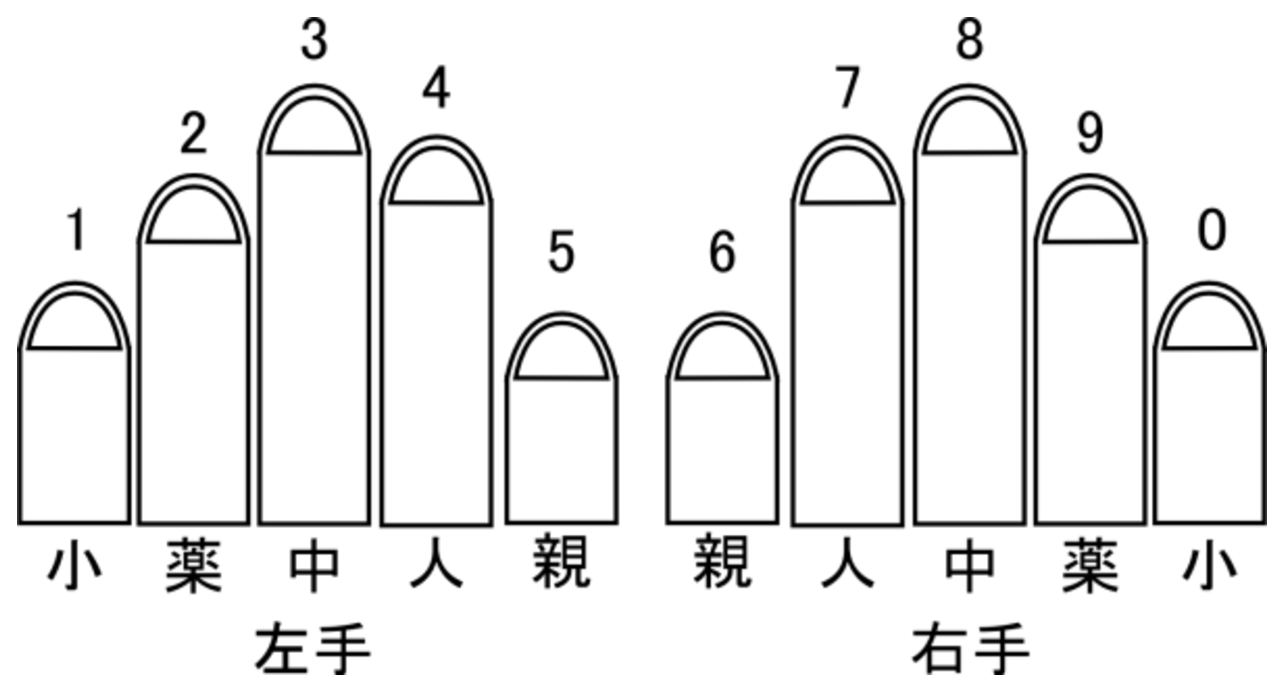
\includegraphics[width=13cm,clip]{res_tomoemon/finger.eps}
\vspace{-4mm}

\part*{�ӌ��Ǝ���}
�{���̎��M�ɂ������Ăł������̊m�F�����Ă��܂����A�뎚�E�E�������E�����������悤�ȕ\���A���e���܂܂�Ă���”\��������܂��B�������Ȃ��Ƃł��\��Ȃ��̂ŋC�Â������Ƃ͎��M�w�ւ��A������������ƍK���ł��B�A���́A�{���̍Ō�ɍڂ��Ă���A���M�w��twitter��u���O�ւ��肢���܂��B

\part*{�ӎ�}
�{���̎��M�ɂ�����A���Z�Ȃ钆�A�����C���^�r���[�ɂ����͂��Ă����������APocari����Adqmaniac����A���ɂ��񂳂�A�ނȂ�������A������AQuvota����A���E�M�m����A�������߂���A�����^���R����AGANGAS����A���ނ���A�����Ėu�N�����c����ɐS��芴�ӂ������܂��B���ɁA�C���^�r���[�̃Z�b�e�B���O���烌�r���[�̎��܂Ƃ߂Ɏ���܂ŁA�����ƂȂ��đS�ʓI�ɂ����͒����� Pocari ����ɂ́A�i�ʂ̊��ӂ̈ӂ�\���܂��B���M�w�����ł͌�邱�Ƃ̂ł��Ȃ����ɖ��x�̍������e�𐷂荞�ނ��Ƃ��ł��܂����B�܂��A���M�w�̗v�]�𕷂��ĕ\���̃C���X�g��`���Ă���������cream����A�T�[�N���������߂�ۂɂ����������O�������Ă����������O�~����Ɋ��ӂ��܂��B���̑��A���M�w�ւ̂����͂��`�ɂ����͂��Ă����������݂Ȃ���A���肪�Ƃ��������܂��B�Ō�ɁA����܂Ń^�C�s���O�Ɏ��g��ŗl�X�Ȍo���ƒm�����c���Ă����������^�C�s���O�E�Ɋւ�邷�ׂĂ݂̂Ȃ���̂������Ŗ{���͊������܂����B�{���ɂ��肪�Ƃ��������܂��B



\clearpage

\tableofcontents

\clearpage

\thispagestyle{empty}
\section*{} % dummy

\clearpage
% 本文のページ番号はアラビア数字でここから1ページ目とする
\setcounter{page}{1}
\pagenumbering{arabic}

\articlepart{Typin' Girls - はじめての競技タイピング}{W/H}

\begin{screen}
過去の記憶がお前に喜びを与えるときにのみ、過去について考えよ。\\
―― Jane Austen
\end{screen}

\section*{序章}

\begin{verbatim}
「いつから」と問われれば、あの日を境に。
僕は君を見ることをやめた。
君と僕のつながりはそうして強まって。
その不可視の糸は、切れることなく今もつながっている。

見やりもせず一心同体となる、一見理不尽な関係が。
日々思い慕いながらも、打ちつけるという関係が。
声こそ聞こえなくても、姿こそ見えなくても。
日々の交流を通して深まってゆくのを感じる。

僕らの交流は、極めて物理的なものだ。
けれど、その実それは極めて言語的でもある。

――物理と言語の界面<インターフェース>。

喩えるならば、それは果てしない大河だろう。
そこに、気が遠くなるような労力をかけ、橋をかける。
決して彼岸に届くことはないと知りつつ、橋をかける。
そんな戯れが、今の僕らの交流の形だ。

とするなら、あの出来事は、七の並ぶ日の夜空のような奇跡だったのだろう。
僕と君が、出会った日を思う。

ふわり、耳元を春風が吹き抜けていった。そんな気がした。

季節は冬。
暖を取らねば震えるような気温の中、懐かしさとかすかな喪失感をも振り払うかのように、洗面器の湯に浸していた両手をタオルで拭う。

ゆるみきっていた姿勢を正す。目がさえる。
ほかほかと熱を帯びた手をそっと、あるべき位置に。
人差し指の腹で、小さな突起をそっとなでる。

意識を、肩に、腕に、手首に、指に、
――鍵盤<キーボード>に。
そして真っ白な雪原に踏み出すように、軽やかに、親指を弾ませた。

カタン。
新雪降り積む窓の外、記憶の扉の鍵<キー>の音。
\end{verbatim}

\section{実力チェック}
\begin{screen}
競えば伸びる。\\
―― Typing Attack の合言葉
\end{screen}

\subsection{タイピング極めました(笑)}

始まりは僕が高校に入った春のこと。

どうしようもないほど位相がずれたインドア青春を送っていた僕だったが、ジュニアじゃないハイスクールに来てとうとう部活というリア充感漂うものに入らなくてはならなくなった。必須だったのだ。

しかし幸いかな、僕にはパソコン部という預言されしメシアがついていた。他の文化部に目もくれず(運動部という存在は、全く、存じ上げません!)メシアに入部届を出した僕は、初日の部活動で度肝を抜かれることになる。

……悪い意味で。

\answer{おじいちゃん先生}{新入生のみなさん。パソコンを使うには、えー、この、キーボード、と呼ばれる、文字の、色々書いてある機械と、マウス、という、ネズミのようなかたt(ry}

\answer{僕}{(レベル低っっっっっっ)}

\answer{おじいちゃん先生}{まずは、日本語を、パソコンに、入力……入力というのは、えー……キーボード、を使って、タイピングを、やるわけですが……入力! この練習から、始めたいと思います。}

\answer{僕}{(トロい! トロイア! トロイア戦争!(←三段活用))}

\answer{おじいちゃん先生}{ローマ字は、みなさん、ご存じですか?}

\answer{僕}{(Yes, I do! 実戦(← 2ch やニコ動への書き込み)で鍛えてる僕に隙はなかった!)}

\begin{screen}
こんなレベルの授業や部活動が実際に行われているところもあるそうで。
筆者の経験では、大学の英語の講義で 2 回に渡り A-Z タイピングをやるだけだったなんてことが実際にありました。英語やろうよ英語……。
\end{screen}

そう、僕は中学の時に自分専用のパソコンを買ってもらって以来、自室で多くの時間をテラワロスなどと打ち込みながら過ごしてきた。タイピングのイロハなんて釈迦に説法。なにしろ僕は、すでにタッチタイプ(キーボードを見ないで打つ超クールなスキルさ)ができないこともない、というハイレベルに到達しているのだよ。

実際、先生の説明することはすべて事前に知っていることばかりだ。IME のオンオフ、ホームポジション、母音と子音、シフトキー……。

退屈すぎて、おもむろにブラウザを立ち上げクオリティを発揮しようかという考えが支配的になってきた……その頃、ようやく面白そうな話になった。

\answer{おじいちゃん先生}{では、もうタイピングができそうだ、という人は、デスクトップにある、この、e-typing という、えー……ボタン、じゃない、アイコン、をダァブル・クリック(←年配の方がカタカナ語を発音するとき特有のテンション)してみて下さい。}

\answer{僕}{(e-typing ……いつだったかちょっとやったことがあったっけ? まあなんとでもなるよ)}

\begin{screen}
スコア帯別のアドバイスが次章にありますので、読者の皆さんでパソコンが手近にある方は、ぜひここで実際に e-typing の「腕試し」に挑戦してみて下さい。\\
\url{http://www.e-typing.ne.jp/}\\
会員登録しないでもトップページから「ランキングタイピング」→「腕試しレベルチェック」と辿ればプレイできます(2011/11 現在)。もちろん会員登録して、ログイン後にプレイしても構いません。
\end{screen}

\answer{僕}{(今週のテーマは「元気が出る言葉」らしい。どんな文章だろう)}

\answer{僕}{(元気出るどころか、なんか、え、つらいけど……? あれ……涙が……?)}

\answer{僕}{(いやいや、集中だ。ザ・アンダーグラウンド・ネットワーク(←2ch やニコ動)で鍛えた秘められし力を解放するときだ……圧倒的スコアを\ruby{叩}{たた}き出せッ)}

カタ……カタ……カタ……。

僕の指先が光の速さで\ruby{迸}{ほとばし}った。\ruby{疾}{はや}い……圧倒的じゃないか我が軍は。

伸ばし棒 \key{-} や位置が悪い \key{B} \key{Y} を打つ所ではさすがに手元を見てしまうが、それ以外はほとんどタッチタイプ。僕のタイピングはタッチ時々チラ見、いいね、いい速度だよ!

\answer{おじいちゃん先生}{ほう! 君はすごいね、映画にでてくる、あれだァ、ハッカァ! みたいだね。}

\answer{僕}{い、いえ……別に……(おおおおおおい気が散るよ! あとちょっとなんだ黙って!)}

ピピッピピピッ。

\answer{僕}{(桂ァ、今何ミス!?)}

……。オツカレサマデシタ。

\answer{僕}{(終わりか……微妙だなぁ、誰かさんの妨害のせいで……)}

「腕試しタイピング」が終わり、結果画面が表示される。

\begin{figure}
 \begin{center}
   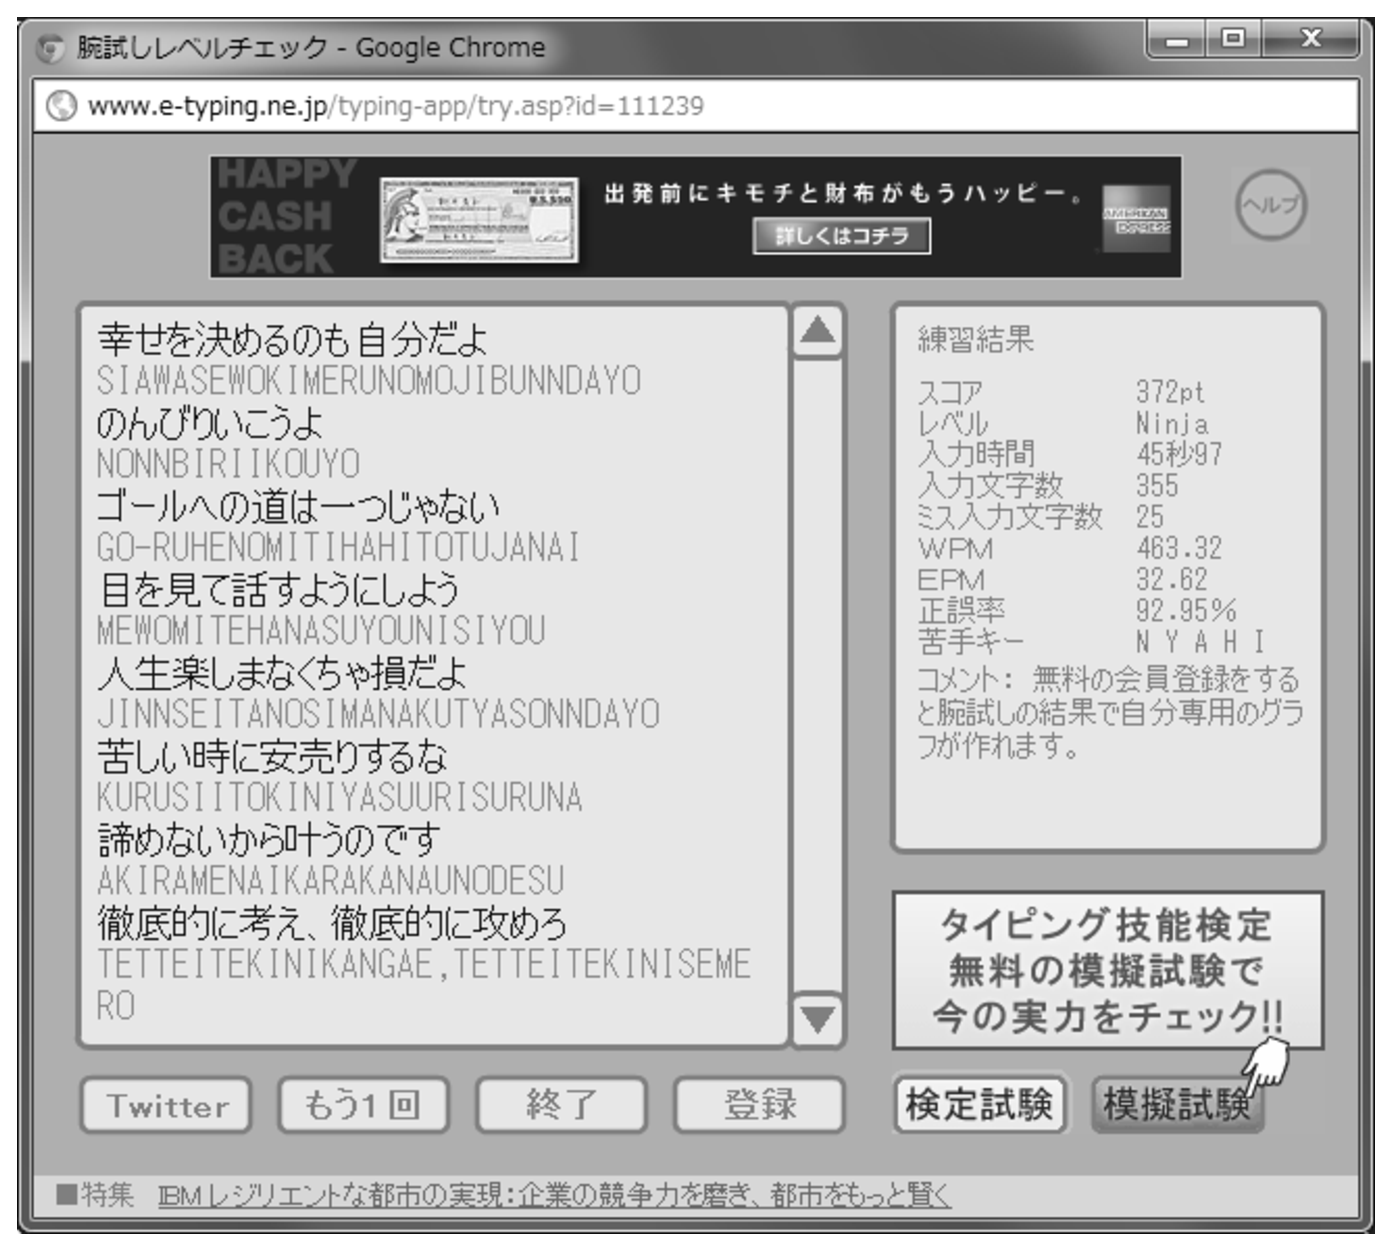
\includegraphics[width=7cm,clip]{res_x_i/ety_result1.eps}
 \end{center}
 \caption{e-typing結果画面}
 \label{x_i:ety_result1}
\end{figure}

\answer{おじいちゃん先生}{ニンジャ! ニンジャ、でましたよ! みなさん、372pt がでました。これはすごい、立派な記録ですよ。もっと速く打てた人、いませんか。}

\begin{figure*}
\begin{screen}
ここらで少々 e-typing について解説を。

最初に e-typing の紹介をしたのは、面倒な導入が不要で手軽にプレイして頂けて、かつ基礎的なタイピング力を見るのに適していると考えたためです。
e-typing の最大の魅力はユーザ数の多さで、ストーリーでもプレイしていた「腕試しタイピング」は毎週ランキングが更新されるのですが、各週のランキングに数千名が登録します。参加者数で見れば、間違いなく国内最大級のサービスです。
「腕試しタイピング」の他にも、入力する文章が様々に異なるモードがあります。「英語」や「長文」、「テンキー数字」など。
また同社が行っている「e-typing master」というタイピングの検定試験もあります。資格としての価値は正直なところあってないようなものですが、数少ないタイピング関連資格ではあるので、趣味でタイピングに取り組む際に目標のひとつにすると良いかもしれません(一番上の級「特級」は我々ガチ勢にとってもそれなりの難易度です)。

スコアについては、「僕」が 372pt で相当調子に乗ってますが、皆さんはどれくらい出るでしょうか。
ちなみに「僕」がプレイしていた「元気が出る言葉」という課題文のセットでは、全国ランキング登録平均スコアが 250pt 程度ですので、実際のところ「僕」のレベルはそれなりに平均以上ではあります。ざっくり偏差値で言うと 60 くらいでしょうか。

この記事は全体として、この時点における「僕」くらいの実力を持っている方を対象にして書かれています。つまり、タッチタイプが完全ではないにしろ\ruby{概}{おおむ}ねできて、実用上困らない程度には速く打つことができる人ですね。副題が「はじめてのタイピング」ではなく「はじめての競技タイピング」なのはそういうわけなのです。
したがって、タッチタイプがままならない方、とつとつとしか打つことができない方に対するフォローは残念ながら十分ではありません。このような同人誌に興味を持つ層であればまず問題ないラインと想定していますが、該当される方はごめんなさい。

なお、e-typing 攻略法については、まもなく登場するヒロインが、次章で解説してくれます。この章はほぼ伏線回収のための駄文だよ。やったね。
\end{screen}
\end{figure*}

だが周りの新入生はまだ黙々と、ピッピピッピと音を立てながら取り組んでいる。まだ打ち終わっていないのだ。

やや離れた所にいた、便乗して取り組んでいたらしき上級生の何名かも、見れば悔しそうな顔……。

つまり、僕の時代か。パックス・オレーノ、来ましたか。

\answer{僕}{ちょっと速すぎましたかね……。}

「ちょっとミスしすぎですかね」と言おうと思ったのに、つい本音が出てしまった。

だがしかし周りからは羨望の眼差し。冷静を装おうとするも、つい頬がつり上がってしまう。

\answer{おじいちゃん先生}{ニンジャ! 君のあだ名はニンジャね!}

\answer{僕}{(UZEEEEEEEEEEEEEEEE)}

こうして初回の部活動が終わった。成果は上々。

こんな感じでタイピングの神として君臨し、統治はせず、つかみはオッケーでゆるーく部活動を乗り切ることができるかと思うと、帰りの足取りは軽かった。というかスキップだった。

\subsection{タイピング界からの使者}

その日の夜、どこぞの運動部のように飯・風呂・寝るの確殺3連コンボを決めるわけがない僕は、帰宅後3秒で当然のように鞄から教科書を取り出し宿題と明日の予習を、やるわけもなく、パソコンの電源を入れ電脳空間へのダイヴ・フェイズへと移行した。

カスタムしてある愛機のログイン画面に、お手の物のタッチタイプでパスワードを\ruby{叩}{たた}き込む。パスワードのような、いつも同じ内容だと打つのがさらに速い。ダカダカダンとパワフルにマジカルにエクストリームに、

\answer{精}{いたたた! いたい、まだ用意できてないですし! ちょっと待っタンマ!}

どこからか声が聞こえた。

まあ、なに、珍しいことでもない。僕クラスになると想像力\ruby{逞}{たくま}しく幻聴が聞こえたりもするのだ。ラノベではないので驚いてやる義理もない。

スルーちからを発揮してダカダカダンとパワフルにマジカルにエクストリームに、

\answer{精}{痛いって言ってますよー無視しないでお願いあいたっ。}

今度は僕の目の前に――否、正確を期すれば、僕のキーボードの上に浮かび上がるように――確かに声の主らしきソレが現前した。

ソレというのはつまるところ、いやつまらなくても、このミニチュアロマン溢れる、ちんまいレディだ。年齢じゃなくてスケールがちんまい。何分の一フィギュアだ君は。

ちょうどキーボードのキーひとつの上に片足が乗るサイズの彼女は、どうも頭を打ったのか、セルフになでなでしながら表情を整えて、

\answer{精}{……ふぅ。気を取り直して、やっほー元気、はじめましてこんばんは。JST 的にこんばんは。}

どうしたことか、幻聴に続いて幻覚まで……などと認識否定を繰り返すのはまだるっこしく、僕もその手のフィクションでイラッ☆とする部分だ。

こんなこともあろうかと! 前々から万一自分の身に起こったらどうするかと、妄想もとい練ってきた策を発動する時がやってきた。僕はこの展開を自らの手で速攻、打破してみせる、速攻――即ちこうだ。

\answer{僕}{――君は霊か天使か女神か選ばれし現代人か異世界人か宇宙人か地底人か未来人か波動生命体か伝承存在か並行世界存在かメタ存在か妄想か脳腫瘍か視覚素子インプラントな拡張現実かオーパーツか人工知能高次元ホログラムか一体ナンデスカッ?}

はあはあと息が上がってしまったが、一気に言い切った満足感で(いやおそらくは酸欠のために)僕は言い知れぬ\ruby{恍惚}{こうこつ}感に包まれた。

そして気づく――死神とかダーク路線が手薄だ。

しかし、この光という光が泡立つ感覚の中魂どっきゅんと昇天するなら、それはありかナ――。

\answer{精}{タイピングの精です。かつタイパーです。typeする人でtyperと綴ります。英語的にはtypistが一般的とか言いっこなしで。}

なかなかやるな……平然と答えてきた。でも。

\answer{僕}{いや待った。自由解答じゃ困ります。上記の選択肢から選びなさい、複数選択可。}

\answer{精}{メタ存在と女神と未来人と並行世界存在と人工知能拡張現実と脳腫瘍がかすっていてあわせて 4 割、残り妄想という感じ? です。}

6割妄想かぁ! やっぱりね! 妄想に妄想ですと自己主張されるあたり、なるほど妄想じみている。

\answer{僕}{妄想メイン……じゃ害はないと? 危害を加える可能性しかないならご退散頂きたいし、危害あるかもだけどオイシイイベントもあるなら詳細聞くし、今すぐオイシイなら頂きますし、特に危なくもオイシクもないなら、自分の存在・文脈・世界設定について語れるだけ語っていって欲しい。僕がどうするかは、その後で決めよう。}

\answer{精}{適応力高すぎで私何も言うことないんですけど……その中では最後になりますか。オイシクなくてごめんなさい。オイシイのは厚くて熱いタイピング同人誌じゃなくて、薄いトリプルエックスなそれを別途お買い求め下さい。\footnote{この元ネタは gummi さんのツイートを参考にしました。勝手に加工・利用してすみません、感謝!}}

\answer{僕}{お買い求め? まあ、そのボディサイズじゃ色々あれだよね……(いや妄想メインならなんとでもなるんじゃ……いやまあ、設定を把握してからにしよう……)オーケー語って。}

\answer{精}{いいんです? ちょっと長くなるかもですよ?}

神妙な顔を作ってうなずく。僕の心が動かされれば、協力を惜しむつもりはない。

こういう不思議存在がコンタクトを取ってくる場合は決まって、何か困っているからだし。

\answer{精}{繰り返しになりますけど私、タイピングのアレです。ことタイピングに関してはエキスパートなタイパーのアレです。なんだっけ……精です、精。私に関して言えば、どこにでもいます。遍在してます。霊的なのです。えへん。で、今はキーボードの上に見えてますよね。半透明ですよね。これは\ruby{憑依}{ひょうい}的なアレで、この物理媒体と計算資源を通してあなたの認識に間接アクセスしています。ハイテクバイオです。えへん。この状態だとキーボードと一体化してるんで……こっちが準備してないのにダカダカと打たれると痛かったり。事実痛かったです。あ、もう大丈夫ですけど。それで、あなたと意思伝達ができてますけど……これは私の力だけじゃなくて、あなたと波長位相的なアレが合わないと無理です。だからあなたは選ばれし(というと聞こえは良いが要は妄想癖の)人的なアレで、ラッキーです。えへん、じゃないか、ぱちぱち。私の核というか本質はもっと抽象的で高次なアレですが、あなたの認識を必要とするという意味では属人的です。……これくらいで、私についてはわかります?}

\answer{僕}{組み合わせはわかった(←見栄)けど……その詳細が知りたいんじゃん。オーバーテクノロジーと証明可能な神秘学を手中に収め現代科学をあざ笑いたい。}

\answer{精}{はい無茶振り頂きました! っていうかそれやったらページ食い過ぎですから! 掘り下げたいのそこじゃないですから! ストーリーめちゃくちゃですから! ……はい、メタです。えへん。で、ですね……掘り下げたいのは「タイパー」の方なんですよう、私はタイパーの精なんですよう、「タイパーって何?」って聞いて下さいよう。}

\answer{僕}{(うわ……口が勝手に……)タイパーって何?}

\answer{精}{厳密な定義はない(諸派あって面倒です……)けど、ここではこう言っちゃいます。「タイピングを入力の手段としてではなくて、目的として行っている人たち」です。これくらい打てれば実用上十分……とかケチなことを言わないで、タイピングそのものを楽しみだしちゃったと。もっと適当に、「タイピングに情熱傾けちゃってる人たち」でも遠からずですね。そのタイパーの代表として私は来ました。すごい無理矢理がんばって、山ほど設定引っさげて、あなたの元へエッチラオッチラ(←こう書くとややエロい)やって来ましたんですよ。なので、言いたいこと言っちゃいます!}

ここまで聞いても、僕は彼女が言わんとすることが読めていなかった。

彼女が僕のタイピングに惚れ込んで、タイピングが世界を救うんだ宇宙で\ruby{隕石}{いんせき}を高速タイピングで打ち落とす人が必要なんだーとかいう話が出てきて、僕がヒーローになるというお花畑を幻視しているのみだった。

――だから割とショックだった。

\answer{精}{ええとですね、まずあなたは調子に乗りすぎなのです。の・り・す・ぎ・な・の・で・す! 井の中の\ruby{蛙}{かわず}です。凡百です。普通です。いや別に普通なのはいいです。でもそれで僕すげーって満足されちゃうと、私がむずむずします。黙ってられないです。世界を見せてやりたくなります。It's a typer world. ブルってる? と言いたいです!}

……何が何だか……わからない……。

タイピングなんかで凄まれる日が来ようとは。それも、こんなデフォルメチックミニチュアガールに。つついちゃうぞ?

\answer{僕}{つ、つまり、タイピングの精として、僕をパニッシュしに来た!?}

\answer{精}{別に罰しないですョ? タイパー優しいです。変人ではあっても愉快な人たちです。あなたはタイピングの基礎力もあって、人と競うことに価値も感じるタイプみたいなので、お仲間になれるんじゃないかなと思って。}

先ほどの凄んだ表情から、一転にこり。

つまりそれは勧誘だった。壮大な展開も、泣ける設定もなかった。

無論のこと、心など動かない。動きようもない。

……そんな風に思っていた時期が、僕にもありました。

\subsection{タイピング始めました}

想像できるだろうか。夕食を終えるなり両親との会話もそこそこに部屋に籠もり、(本人\ruby{曰}{いわ}く)半分オーバー妄想らしい存在と盛り上がる、(主に頭が)かわいそうな年頃の学生の姿を――僕である。

\answer{精}{お腹もふくれましたところで、現実を直視して頂きたいと思います。}

\answer{僕}{いや今というまさに今、妄想を、非現実を直視してるけど……。}

\answer{精}{\ruby{刮目}{かつもく}せよ! これが全・日・本レベル! 私の還る大・海・原! です! じゃん!}

\begin{figure}
 \begin{center}
   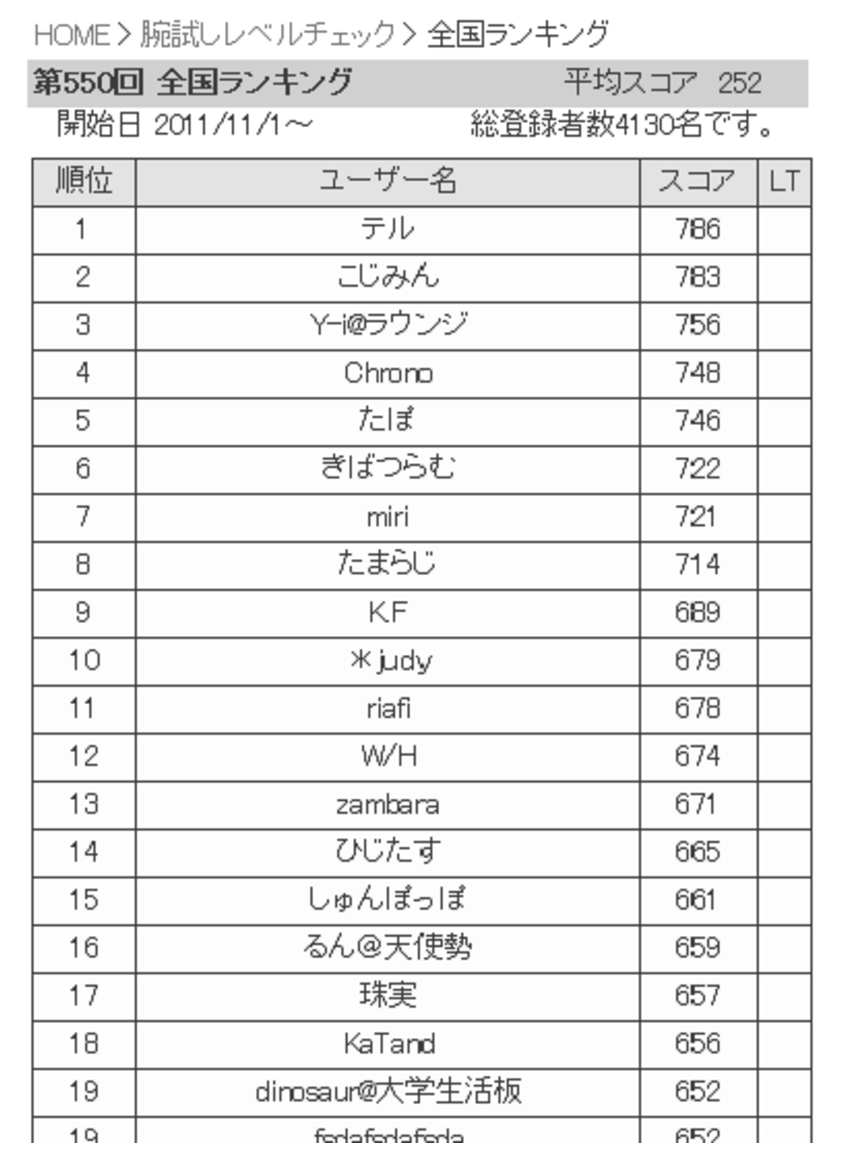
\includegraphics[width=7cm,clip]{res_x_i/ety.eps}
 \end{center}
 \caption{e-typing腕試し全国ランキング}
 \label{x_i:ety}
\end{figure}

\answer{僕}{えええええ!!(←約一名の自室に響き渡る近所迷惑な声)}

……ってなんすかこれ。一瞬でリアクションできる凄さ、どこにもないっていう……。テンション合わせてあげた僕、アホの子みたいっていう……。

\answer{精}{全・日・っp}

\answer{僕}{いやもうそのテンションいいんで、解説を。}

\answer{精}{はい。(←真顔)これは、学校であなたが打って 372pt を\ruby{叩}{たた}き出していた e-typing 腕試しモードのスコアの全国ランキングです。週ごとにリセットされるので、歴代のランキングとかじゃなくて、その週に出された記録しか入ってないですけど。}

\answer{僕}{わーすごい(←真顔)。チート使いばっかで荒れてる。}

\answer{精}{え、チート違いますよ?(←真顔)ガチですガチ。ガチタイパー勢です。}

\answer{僕}{いやだって……え?(←変顔) ウソでしょ? トップで 500pt とかだろ常識的に考えて……。}

一位のやつ、僕の倍以上スコアあるって?

大体、700 超えは若干名しかいないのに、600 後半はたくさんいるってのは……。

あれ? ってことは 600 後半の団子はガチってことに……いやいや 600 って…… 600!?

\answer{僕}{一位はチートじゃ? 「テル」って「チート」の変形もじりで自主申告してるし。}

\answer{精}{断じてチートじゃないですよう。現代の生きる伝説テル・ぶったーさんになんてことを……。}

\answer{僕}{え、でも……うーん……まあ、600 くらい出せる人がいるのはわかった。700 とかは眉唾かな。}

\answer{精}{(歴代トップだと 800 オーバーですけど……)いいでしょう、600。}

\answer{僕}{それくらいだったら、僕もやれば出せそうだけど。}

\answer{精}{今のままじゃ無理無理、絶対無理。っていうか、600 って私もそれくらいですし。}

\answer{僕}{え? そういえば君もタイパーって言ってたっけ。……出せるの? ってそのボディサイズじゃ無理じゃね?}

\answer{精}{見たいです?(←見せたくてうずうずしてる) 方法があるんですよー、これが。じゃあちょっと、お手をこちらへ。}

言うなり、キーボードの上からこっちこっちと手招く「精」(こいつ結局名前なんなんだ)。

先に説明すればいいものを、にこにこしたまま、黙って彼女は僕の手に触れシュイィーン! シュイィーンって!? シュイィーンって!!!

僕の肩から先の感覚はすぅっと、ろうそくの火でも吹いて消すかのように消えてなくなった。

\answer{僕}{ヴぁうおぁあああああああ腕がぁああああ! 僕の腕がぁああああああああああ!}

\answer{精}{あ、ごめんなさい。うずうずしちゃって説明が遅れました(てへっ)。こうやって\ruby{憑依}{ひょうい}すれば物理的に打てるなぁと……。}

見れば、確かに、腕は、ついている。

取れていない。痛みはない。

\answer{僕}{あああ……はうわっ、うおゎ、ぅわーお……(←目がマジ)。}

\answer{精}{一時的に借りてるだけですよ。ちゃんと戻せるし戻すので、そんなに焦らなくてだいじょぶです。目がマジにならなくてだいじょぶです。セーフです。}

\answer{僕}{お、オーケィ……。}

とは言ったものの、額には冷や汗が残る。いや、だってこれ、\ruby{憑依}{ひょうい}って……この感覚、普通じゃないよ。アブノーマルよ。妄想 6 割とか言ってたから油断しきってたっての……彼女の気分次第じゃ実害ありまくりじゃない。

だが当の彼女はというと、

\answer{精}{非ログイン状態でいっかー、おっけー、元気ワードね。実は長いだけで打ちやすさそんなでもないけど……ワード末尾の「できる」とかカモってるし、ま 600 は何度かやれば……!}

ノリノリである。本当にうずうずしていたらしく、僕はアウトオブ眼中。

\answer{精}{じゃ打ちまーす。}

感覚がない僕の腕から下が、僕の意識を通さず勝手にキーボードを操作していく。僕の手でありながら僕の手ではないという奇妙な体験。

この\ruby{憑依}{ひょうい}現象に文字通り全身全霊でびびって震え上がった僕は、彼女の気分を損ねないように、適当にスゲーとかヤベーとか言おうとヒヨっていて。

そして――言葉を失った。

ッタカタタタタタタタタタタタタタン!
ッタカタタ(ピッ)タタタタタタタタタタタタタタタタタタタン!
ッタカタタタタタタタタタタタタタタタタン!
ッタカタタタタタタタタタタタタタタタタタタタタタタタタタタン!
ッタカタタタタタタタタタタタタタタタタタタン!

音は弾倉交換しつつ撃ち続ける Machine gun なら、

手もコンピュータと同期し動き続ける Machine だった。

僕の手が勝手に動くという、恐怖感。僕の妄想でチートだろうという、非現実感。僕も何度かやればこれくらい出せるという、お花畑。それらがマシンガン音と残像の見えそうな指の高速移動に、撃ち抜かれ圧倒され吹き飛ばされる。

打ち終わって、一息ついたらしき彼女にかけるべき、いくつかの言葉が浮かんだ。

「ゴッデス! 君のあだ名はゴッデスね!」

「ちょっと速すぎますね……」

「Is it a typer world? 狂ってる……」

だけど、実際に口をついて出てきたのはこれだ。

\answer{僕}{タイピング、始めたいです。}

\begin{screen}
主人公と同じ気持ちになりたい方は、動画サイトにある高速タイパーのプレイ動画を見ましょう。
以下にいくつかおすすめのものを載せておきます。どれも魂が抜けるレベルです。

\begin{itemize}
 \item (ニコ動) sm8243869 あきうめ氏の「慣用句」798pt
 \item (ニコ動) sm13155297 あきうめ氏の手元
 \item \url{http://youtu.be/4YzFkzRbOcg} ひろりんご氏の「思い出の言葉」810pt
\end{itemize}
\end{screen}

\section{e-typingで基礎力を}
\begin{screen}
ミスをするくらいなら打つな!\\
―― 正確性重視を強調する、全日本タイピスト連合のキャッチフレーズ
\end{screen}

\subsection{敵を知り己を知らば}

無事に腕の制御を取り戻した僕は、早速彼女の話に耳を傾けていた。

\answer{精}{まずは姿勢です、そのやる気ない感じのそれをなんとかして欲しいです。}

\answer{僕}{なるほど把握、姿勢が重要なのは何やるにしても基本だね(シャキッ)。}

\answer{精}{いや現段階だと姿勢とか誤差です。}

\answer{僕}{と、言うと?}

\answer{精}{座学やるので、まじめに聞いて欲しかっただけです。}

\answer{僕}{あ、はい。}

\answer{精}{敵を知り己を知れば百戦危うからず! ……と偉い人は言いました。ということで、自分ってどれくらいの腕前だと思います?}

\answer{僕}{ふむ……けっこうすごいと思ってたんだけど。}

\answer{精}{そうです、けっこうすごいです、実際。}

\answer{僕}{こき下ろしたり持ち上げたり、どっちなん打!(あれ、なんだこのカンジ……)}

\answer{精}{一般人的には「すごい」んです。だって普段文字を入力するときに困ることなんてないでしょ? これなら。}

\answer{僕}{そういう意味じゃそうかな? ネトゲでチャットするのも、ブログ書くのも楽勝だしねぇ。}

\answer{精}{そう、普通にパソコンを使う時の入力手段としてなら、十分です。}

\answer{僕}{でも……さっきのあれ見ると、まだまだかなって。}

\answer{精}{ここから先は、言ってしまえば、基本的に遊びの領域です。文字の入力をお仕事にでもしない限り、見返りはあまりありません。だから「競技タイピング」と言っています。}

\answer{僕}{技を競うって書いて「競技」か……。}

\answer{精}{100m を 13 秒で走れる人が、がんばって 10 秒で走れるようになっても、そんなの日常生活ではほぼ何の役にも立たないですよね。でも陸上選手から見たら、その差はものすごいですし、10 秒で走れる人には賞賛が送られます。スポンサーもつくかもしれません。つまり陸上という世界の中では「10 秒で走れる」という、そのこと自体に価値があるわけです。私たちのいる競技タイピングの世界も、陸上と比べちゃうと小規模ではありますけど、そういう場所です。だからさっきは「井の中の\ruby{蛙}{かわず}」なんて言い方をしましたけど、井の中は井の中で快適です。困らないし、悪くないです。引き返すなら今のうち……ですよ?}

\answer{僕}{井戸ごと海に放り込んだのは誰ですかね……でも、いいよ。とりあえず君の記録はすぐ超えてみせるから。}

\answer{精}{わー、その意気やよし! やはり私の目に狂いはないですね。}

「役に立たない」と断言されて興味を失う人もいるんだろう。

でも、それを言ったら、僕の普段プレイするゲームだってそうだ。音ゲーがうまくても、FPS がうまくても、基本的に役に立たない。でも、楽しいからやる。

楽しいと思えるうちはやってみよう――それが僕の出した回答だった。

\answer{精}{では、仕切り直して、次は敵を知ります。解説のため、あなたが調子に乗りまくっていたニンジャ記録の重要部分をぺたっと。}

\begin{figure}
 \begin{center}
   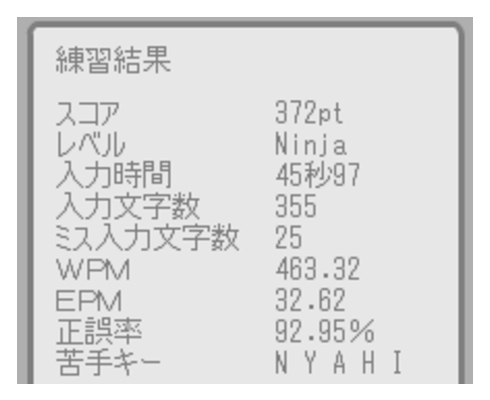
\includegraphics[width=7cm,clip]{res_x_i/ety_result2.eps}
 \end{center}
 \caption{結果画面の重要部分}
 \label{x_i:ety_result2}
\end{figure}

\answer{僕}{あれ、結果画面左の部分は見なくていいの?}

\answer{精}{左にはワードが並んでいるだけですからね、今は注目しないでいいでしょう。}

\answer{僕}{ワード?}

\answer{精}{タイピングゲームでの出題文のことです。英単語の word の意味通りに「単語」とは限りません。例えば、この e-typing なら、画面にひとつずつ文章が表示されますよね。この文ひとつひとつが{\bf ワード}と呼ばれます。まあ、ちゃんとした定義はなくて曖昧な感じですけど。ノリです、ノリ。}

\answer{僕}{なんとなく把握した。}

\answer{精}{ちなみに e-typing ではランダムに 15 ワードが出題されます。意味、わかりますよね。}

\answer{僕}{何か文章が表示されて、打って……と 15 回やったら終わりになる、と。}

\answer{精}{です。では各項目を解説しましょう。それぞれこういう意味です。}

\begin{itemize}
 \item スコア:結果から計算されたスコア。これで競う
 \item レベル:スコア帯に応じた称号
 \item WPM:一分間に何回正しいキーを打つスピードか
 \item EPM:一分間に何回ミスをするペースか
 \item 入力時間:入力を受け付ける状態だった総時間
 \item ミス入力文字数:ミス(誤打鍵)をした回数
 \item 入力文字数:正しく打った文字の数
 \item 正誤率:1 - ミス入力文字数 / 入力文字数
 \item 苦手キー:ミスが多かった部分のキー
\end{itemize}

\answer{精}{まず WPM が一番注目したくなりますね。}

\answer{僕}{タイピングの速度か。僕は一分間に 463 回、ってことは 60 で割れば……一秒間に 8 回弱。やっぱかなり速いよね。}

\answer{精}{ですね。最初は秒速に直して考えた方が大体のスピードがわかりやすいはず。でも、タイパーの人達は分速の方に慣れてます。その方が整数で表現できたり、大きい数になるので差がわかりやすかったり、メリットがあるので。まあ心配しなくても、多くのソフトでこちらが使われているので、そのうち分速の方に勝手に慣れますよ。}

\answer{僕}{EPMはWPMのミスタイプバージョンか。}

\answer{精}{正直なところ、あまり注目することはないですね。というのも「ミス入力文字数」も表示されるので、普通はこっちに注目します。}

\answer{僕}{これは単にミス回数だよね。}

\answer{精}{そうですけど、「何カ所でミスをしたか」ではないことに注意です。同じ部分で何回も間違ったキーを押すと、一回ずつこの「ミス入力文字数」にカウントされちゃいます。}

\answer{僕}{何回「ピッ」ってなったかってことね。「入力文字数」は……正しく打った文字の数ってことは、出題されたワードによって決まってくる数。}

\answer{精}{ほぼその考えで合ってますけど、実はちょっと違います。が、これはディープな話なので後回しで……「入力時間」「正誤率」についても、なんとなくで大丈夫です。}

\answer{僕}{「苦手キー」は間違って押したキー?}

\answer{精}{ではなくて、ミスをした箇所で押さなきゃいけなかったキーです。あなたの記録の場合\key{N},\key{Y},\key{A},\key{H},\key{I}を押さなきゃいけない場所でミスが多かったというわけ。}

\answer{僕}{レベルはスコアで決まるんだよね。最高のレベルまではやりたいところ。}

\answer{精}{その発想は……フフフ、危ないかと?(暗黒微笑)そしてお待ちかねのスコア計算式ですが、こうなってます、ででん。}

\begin{screen}
スコア = (WPM - EPM) $\times$ 正誤率の二乗
\end{screen}

\answer{僕}{へぇ。WPM - EPM が 430.7 だから、これに 0.9295 を二回かけて……372.111986675。確かにスコアの 372pt に合うね。}

\answer{精}{ここからわかることはなんでしょう?}

\answer{僕}{うーん……スピードが速いとスコアが高くなる。}

\answer{精}{当たり前すぎますけどね。……むしろ、速度である WPM をベースに、そこからしょっ引かれていくという見方が重要かな。もし引かれなければ、WPM がそのままスコアになるわけです。}

\answer{僕}{EPM が 0 で正誤率が 100\% なら、WPM がそのままスコアか。それってつまり……一回もミスをしないってこと。}

\answer{精}{Exactly(その通りでございます)。EPM も正誤率も、ミスに関係した数ですからね。ミスをすると EPM が増えて正誤率も下がる。しかも正誤率は二乗で計算されちゃうので……イメージとしてはミスのペナルティが三重につく感じです。三重苦です。}

\answer{僕}{この記録 25 回もミスってるじゃん(主に誰かのせいで……)、もしこれがなかったら、WPM がそのままがスコアで、463pt!}

\answer{精}{ミスが多すぎます。はじめからやり直してください。ミスをしないということは、ミスをしたことに気づいて打ち直す……っていうタイムロスもなくなるということです。だから今のあなたの場合、実はノーミスなら WPM も上がる余地があるってこと。}

\answer{僕}{500pt 完全に見えたよ、これ。}

\answer{精}{さあ、それはどうでしょーかね?}

キーボードの上に陣取る妄想生命体(なのか?)は、謎の笑み(=暗黒微笑)を浮かべるとそう言い残し、姿を消した。僕の目の前には、明け渡されたキーボード。

よし、やってやろうじゃないか。500pt の壁、速攻打破してみせる。ミスをしなければ大丈夫だ、問題ない。

\subsection{何戦してもまだ危うい}

それから数日が過ぎた。

あの日はどうも疲れていたようで、あれ以来、腕の感覚がなくなることも、おかしな幻覚・幻聴を体験することもなくなった……という展開になる可能性を 50\% 程度と想定していた僕だったが、現実は妄想に寛容だったらしい。今日も、部屋には打鍵音が響き渡っている。

\answer{僕}{……(ピッピッ)くそ……またミスって詰ま(ピッ)ってミス(ピッ)って詰まって……(ピピピッ)うううう!}

未だに 500pt を出すことはできていない。それどころか、450pt すらも出ていない。

\answer{精}{急ぎすぎなんですよ。}

\answer{僕}{でも、このスピードじゃないと……何度もやれば 500pt が出るはずなんだよ。奇跡が起きれば。}

\answer{精}{気持ちはわかりますけど、さすがに絶望的です。そろそろ気づいてるんじゃないですか? ある程度スピードを落とさないと、ノーミスなんて出ないって。}

\answer{僕}{ノーミスならスピードも伸びる余地があるって言ったの君だ! だまされた! うぼぁー!}

\answer{精}{言いました。言いましたが、今回すぐそれが達成できるとは言ってません……つまり、達成は 10 年後、20 年後ということも……。}

\answer{僕}{ひょおおおおおおおお!}

\answer{精}{という冗談はさておき。}

\answer{僕}{はい。(←ノリに慣れてきた)}

\answer{精}{エンジン全開で打って、運良くミスがなかったら……なんていう妄想的な打ち方をしていると e-typing は永遠に、アレです、クソゲーです。イライラ棒です。だからその逆、ミスを極力しないような打ち方で、どれだけスピードを出せるか、と考えるといいです。}

\answer{僕}{やってみるか……。}

\answer{精}{プレイ中に\key{Esc}キーを押すとプレイ中止、結果表示画面で\key{R}キーを押すとリトライできるので、活用してください。}

\answer{僕}{いや、それ最初に言ってよ……。}

―― 十数分後 ――

\answer{僕}{やっと出たし……ノーミス。}

\answer{精}{めでたいです。スコアは……。}

\answer{僕}{340pt。ダメじゃん! 最初の記録よりも下がってる! ゴミ過ぎる!}

\answer{精}{ミスをしないように打つのがいかに難しいか、わかったんじゃないですか。滅茶苦茶に乱打してノーミスなんて奇跡は、まずないんです。}

\answer{僕}{悔しい……けど感じちゃう……その通り。ミス数を抑えようとして打つと、すごく遅くなる。ビクビクして、速く打てないっていうか……。}

\answer{精}{(この歳にしてこのネタ根性……)でも、そこで無理して指を動かすと、ミスになっちゃいますよね。}

\answer{僕}{それそれ。でもじゃあ、速くてノーミスって……どうやるの?}

\answer{精}{魔法のような解決策はないです。でも、練習をすると、だんだんできるようになります。さっきも言った通り「ミスをしない範囲で速く」という意識でタイピングをすることは重要です。今はノーミス縛りでやってもらいましたが、必ずしもノーミスである必要はないですよ。はじめはミス 3 回までとか、それくらいを意識するだけでも十分、効果があります。}

\answer{僕}{そんなこと考えてタイピングをすることなんて、普通ないしね。}

\answer{精}{普段のタイピングシーンでは「適当に速く打ってミスしたら直す」か「速度は気にせず、丁寧にゆっくり打つ」かどっちかなんです。「速くて正確ぅ!」\footnote{元ネタは「バトル&ゲット! ポケモンタイピングDS」。}できれば最高なんですけど、なかなかそれは意識しませんよね。}

\answer{僕}{それを目指すなら、初心にかえって練習あるのみってことか。}

\answer{精}{そう。そしてそういう意味で「速くて正確ぅ!」なクールなタイピングの基本を身につけるには、e-typing のスコアルールは割と、ちょうどいいんです。ノーミスで打ってさえいれば伸びるというわけでなし、ミスを増やしてでも速く打てば伸びるというわけでなし。両立ができた時、良いスコアが出るようになっています。もちろん、運の要素もありますけどね。そこはゲームですから。}

\answer{僕}{意外と奥が深いから困る。}

\answer{精}{この程度で奥が深いなんて言っていたら……気絶しますよ?}

\answer{僕}{楽しみにしとく。}

と言ってしまってから、本当に楽しみにしている自分に気づく。

この時の僕は、わかったようでいて、何もわかっていなかったのだ。踏み込もうとしている世界が、一体どのような魔境であるのかすら。

\subsection{段階別攻略}

僕は正確性を重視して練習を重ね、とうとう 3 ミス 440pt という記録を出すに至った。ミスがなければ 450pt 超え。悔しさはあったが、もう 450pt は時間の問題だと確信できる。

そして同時に、500pt を改めて意識する――。

\answer{僕}{一番いい助言を頼む。}

\answer{精}{いろいろな要素がありますからね……段階によって大まかにアドバイスになりそうなことはありますが、個人差もありますし。読者さんのこともありますので、段階別に色々と見てみましょか。}

\subsubsection{~200pt}

\answer{僕}{じゃ、100pt とか 150pt とかの雑魚は?}

\answer{精}{言い方はどうかと思いますけど……でもごめんなさい、そういう方には練習してくださいとしか。パソコン入門的な本や初心者向けのタイピング練習サイトを参考にするのもいいですし、別に参考にしなくても、ひたすら打っても伸びる頃だと思います。e-typing にも「腕試し」の他に「基礎練習」「基本練習」のようなコンテンツがあるので、試してみるのもいいですね。}

\answer{僕}{キーの位置を覚えたり、ホームポジションからの動かし方を練習したりするやつね。}

\answer{精}{面白みがあまりないので軽視されがちですけど、伸ばし棒\key{-}や\key{P},\key{Z}みたいな小指の方にあるキーと、あと人差し指で幅広くカバーしなきゃいけない中央付近のキーは、後々まで苦手意識が残りやすい部分です。もっと速く打てている人でも、不安があったら良い機会だと思って練習しましょう。}

\answer{僕}{さすがに僕にそれは当てはまらないな。(←ハイフンのたびに減速してる人の台詞)}

\subsubsection{200pt~300pt}

\answer{僕}{250pt くらいが一般の人の平均らしいけど、このへんは?}

\answer{精}{そうですねぇ、例えば「き」なら右手中指で\key{K}\key{I}という風に打ちますよね。こういうひらがな単位での運動は、反復練習して無意識にできるようにすることが大事です。別にまだキーボードを見ていてもいいので、無意識に、ひらがな単位でまとめて。}

\answer{僕}{250pt もあれば、それはとっくにできるんじゃ?}

\answer{精}{かもです。個人差があるって言葉でお茶を濁します。ひらがな単位でまとめて打てるなら、今度は単語とかのレベルの「まとまり」を意識して練習するといいです。}

\begin{screen}
\begin{itemize}
\item[ ] みかんをたべる
\item[×] み/か/ん/を/た/べ/る
\item[○] みかん/を/たべる
\end{itemize}
\end{screen}

\answer{精}{このように認識しやすい単位に分けて、各部分はスムーズに打てるように。最初から「たべる」の 6 打鍵 TABERU をまとめては難しいかもしれません。その場合は TABE で 4 打鍵とか、もう少し細かく分けた所からスタートでもいいでしょう。ひらがな単位よりは長い部分を一気に、というのがポイントです。}

\answer{僕}{e-typing を始める前から気づいたらやってたな。}

\answer{精}{ある程度速く打てる人は、必ずこうやっています。できるようになると一気に速くなりますね。}

\answer{僕}{他には?}

\answer{精}{このスコア帯の人に限らないですが、ここから先は「もっと速く打とう」と意識して打たないと伸びていかないと思います。実用的な目的でタイピングをしている人などは、この程度のスピードでも特に不自由しないので、「タイピングとは、これくらいのスピードで考え、指を動かすもの」って速度の制限を無意識にかけてしまっていることがあります。もっと速くなりたいなら、ハングリー精神を持ちましょう。大丈夫、あなたの限界は全然こんなところじゃないです。}

\subsubsection{300pt~400pt}

\answer{僕}{300pt 以上ってなると……練習を始める前の僕くらいか。じゃ、この間言われたことの通りなのかな。}

\answer{精}{そうですね。タイピングに特化した練習はしたことがないけど、パソコンはバッチリ! 系の人はこの辺じゃないでしょうか? 繰り返しになりますが、焦りすぎず、正確性重視で打ってみることをオススメしたいレベルです。初めからノーミスなんていう人は少なくて、400 WPM 以上出ているけど、ミスのペナルティのために 350pt 程度、という人が多いですし。}

\answer{僕}{僕もそのタイプだったわけだ。あとこれさ、やっぱり慣れもあるよ。ワードの種類ってそんなに山ほどはないから、何度も何度もやってると打ち方がわかってくる。}

\answer{精}{週ごとにワードのお題、ワードセットが変わりますが、各セットは 100 から 500 種程度のワードからなってます。多いと思うかもですが、打っていればすぐ見たことのあるワードばかりになっちゃいます。ワードごとの癖が把握できていれば、もちろん打つのも速くなりますし、スピードを出せるワードはどれか、ミスしやすいワードはどれか、なんていう意識・調整もしやすいわけです。そうやって慣れることを{\bf ワード慣れ}と言っていて、もちろん重要ですね。}

\answer{僕}{それでけっこう伸びた感じがする。}

\answer{精}{ひとつ前で解説した、まとまりで認識、ということに関連して、{\bf 先読み}と呼ばれる技術もそろそろマスターしたい頃です。}

\answer{僕}{あーあ、イケてる名前の技が出てきちゃいましたね……僕の時には言わなかったくせに……。}

\answer{精}{いじわるじゃないですよ? あなたの場合は最初からできていたのです。名前は荘厳ですけど、実は大したことじゃないので。常に今打っているところの少し先にまで目をやってワードを読んでおいて、打鍵が途切れないようにする技術のことです。}

\answer{僕}{それかぁ……確かに最初からできたよ。}

\answer{精}{e-typing のように文章形式でワードが出てくる場合は、先読みが特に簡単ですからね。別の競技だとワードが単語単位だったりするので、その場合はまたちょっと訓練が必要です。}

\subsubsection{400pt~500pt}

\answer{僕}{やっと今の僕のレベルだ。}

\answer{精}{一般人的速いライン 400pt から、タイパー的 500pt の壁まで……色々な攻略が考えられる時期です。一つには後半加速という要素が大事になってきます。各ワードのはじめの部分は、まだ速く正確に打つのが難しいと思います。でも、後ろの方は頑張ると速く正確に打てるはず、という考え方です。}

\answer{僕}{どうして後ろは速く打てるわけ?}

\answer{精}{詳しくはまた改めて解説しますが……「各ワードの打ちはじめの所が難しい」というのは実感しませんか?}

\answer{僕}{確かに、はじめの数文字で急ごうとするとミスになることが多いか? 手を急に動かすのがキツいのかな。}

\answer{精}{それもありますけど、ワードが表示された瞬間は、そのワードが一体どういう文章なのか? 最初の文字は何か? とかで頭がいっぱいじゃないですか。でも、後ろの方を打つ頃には、先読みをしていれば、もう頭の中でワードが読み終わっているので。}

\answer{僕}{打つことに専念できるってことか。}

\answer{精}{はい、とりあえずそういう理解で良いと思います。ワード慣れとも関係しますね。何度も何度もそのワードを見て打ったことがあれば、より一層読む必要がないじゃないですか。百人一首で、上の句の途中まで聞いただけで、下の句まで全部わかってしまうような感じで。}

\answer{僕}{ちょっとわかる。}

\answer{精}{このあたりからは、やり込んで体で理解しないと、頭だけじゃわからないかもしれません。他にもワードをまたぐ際のリズム感ですとか、ワード慣れを徹底して加速できるワードでは攻めていくとか、言えることはありますが……どれも説明だけで理解するのはキビシイんじゃないかと。そういう意味で 500pt あたりに壁は実際にあると思いますです。}

\answer{僕}{基本的には実戦あるのみか。}

\answer{精}{e-typing だけで 500pt 以上まで鍛えようとするのは、正直つらいかも。次章以降で紹介する他のソフトも使ってベースになる速度を底上げしつつ、目標のひとつとして取り組むのがおすすめですね。逆に言えば、基本的な速度が十分あって、正確に打つこともできるなら、e-typing に特化した練習はしたことがなくても 500pt は出せます。}

\answer{僕}{じゃあ、500pt より上の世界は?}

\answer{精}{競技タイピングに特化した練習をしたことがないのに 500pt なんて人はほとんどいません。だから、ほぼ全員タイパーの世界ですね。やっほーみんな見てるー? 晴れ舞台だよー! と言いたいです。}

\answer{僕}{とか言ってごまかして、教えないつもりでしょ。}

\answer{精}{入門者に語るような話じゃないと思って、遠慮しただけですよ? でも興味があるなら……ついでに紹介しちゃいましょう。あなたはその方が燃えるタイプみたいですし。}

\subsection{行きすぎた攻略}

キーボードの上に鎮座していた「精」は立ち上がると、僕に背を向けて大きく呼吸した。これからすごいことを語るよという、要らない演出だ。

\begin{screen}
しかしこの節は、脅しではなく本当に敷居が高いです。
自信のない方は飛ばして読んだ方が、むしろスッキリするかもしれません。
ストーリー的にも何も進展はないので、気軽に飛ばしてください。
\end{screen}

\answer{精}{まず、ここから先のレベルを目指すには基本的な打鍵速度も絶対に必要です。反復練習も必要になりますし、攻略法を知っただけでどうこうなるものではないです。}

それは、450pt 目前まで取り組んだ僕もすでに感じていることだった。自分を鍛えないとどうしようもない。攻略法のような情報は、そのための道しるべでしかない。

\subsubsection{ワード先頭部分の高速化}

\answer{精}{ここまでのレベルとの最大の違いは、いわゆる初速と呼ばれる要素が重要になってくる点です。「はじめの部分は速く打てない」とさっきは諦めたようなことを言いましたが、そこを切り崩さないといけません。最初の一打までにかかる時間が短く、かつ最初から最高速で打ち始めるのが理想です。}

\answer{僕}{最初の一打までの時間……?}

\answer{精}{はい。私は{\bf レイテンシ}と呼んでいます。この時間のこと自体を{\bf 初速}という人もいますね。この要素の重要性については、こういう図を書くとわかるんじゃないでしょうか。e-typing の慣用句というテーマに「\ruby{匙}{さじ}を投げる」というワードがあって、私が打つとこんな感じの結果(図\ref{x_i:ety_bar})になります。}

\begin{figure*}
 \begin{center}
   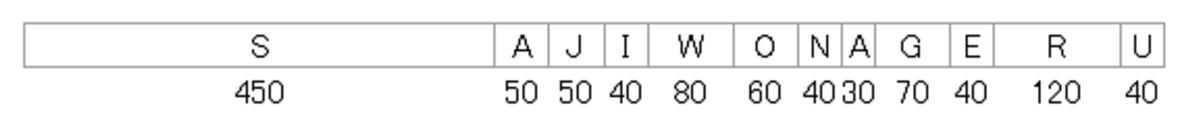
\includegraphics[width=14cm,clip]{res_x_i/ety_bar.eps}
 \end{center}
 \caption{文字ごとの打鍵時間}
 \label{x_i:ety_bar}
\end{figure*}

\answer{精}{見方はわかりますよね。各文字を入力する際にかかった時間が、その部分の横幅に対応しています。数字の単位は ms(ミリ秒、1/1000 秒)ですね。}

\answer{僕}{最初の\key{S}でかすぎだろ、常識的に考えて。}

\answer{精}{初めのキーは\key{S}じゃなくても、どんなキーでもこういう結果になります。打鍵速度が遅いうちは気になりませんが、後ろの部分の打鍵速度がこれくらい速くなっていると、むしろここが重要というわけです。}

\answer{僕}{450ms って……これはどうなの? 遅い方?}

\answer{精}{これも個人差がすごくあるんですが、特に訓練をしていないタイパーで 450ms から 500ms 程度だと思うので、並ですね。今のあなたのレベルだと……平均 500ms 以上はかかるかな。}

\answer{僕}{……でもこれは 100ms とかには絶対ならないよね。反射神経的にさ。}

\answer{精}{訓練すると、平均 400ms に持っていくことは誰にでもできると思います。そして初速・レイテンシを重視して記録を出しているトップランカーともなれば 350ms 程度がバシバシ出せます。数字だと僅かな差に見えるかもしれませんが、ワードが短いと、これだけで 50pt とか 100pt とかの点差につながります。さっきの図、再度凝視してみて欲しいです。後ろの部分はかなり極まってます。ここを速くして 50ms 縮めるのは厳しい。でもレイテンシなら、それくらいは削る余地があります。}

\answer{僕}{もしレイテンシが 350ms になれば全体で 100ms 分短くなるから……割合で見ても相当速くなるね。どうやったら鍛えられるの?}

\answer{精}{一番重要なのは{\bf ローマ字読み}と呼ばれるスキルを身につけること。「\ruby{匙}{さじ}を投げる」の方ではなくて、「SAJIWONAGERU」というローマ字表記された方を読み取って打つんです。}

\answer{僕}{なるほど、「\ruby{匙}{さじ}」を読むのにかかる時間がもったいないってことだ。「S」ならそのまま \key{S} って打てる。でも、一打目はともかく、その先までローマ字読みで速く打てる気はしない……。}

\answer{精}{はじめからローマ字読みをしていたという人もいますけど、訓練で後から身につけることもできます。一朝一夕には無理ですけどね。初めだけローマ字読みして、ワードの半ばからは漢字かな交じり文の方を読む人もいますし。}

\answer{僕}{今すぐは手がでないな……他には?}

\answer{精}{反射神経を鍛えるため、右脳的なトレーニングをすることも効果がありそうです。瞬間的に判断する脳の働きを鍛える感じでしょうか。}

\answer{僕}{それは才能というか、生まれつき決まってるんじゃ……?}

\answer{精}{「反射神経」と言うと、そういう神経があって、生まれつきみたいに思っちゃいますけど、生物学的にそんな神経はないですし、陸上選手だって卓球選手だって、後天的に鍛えてますよね? 才能のような要素がゼロだとは言いませんけど、そう言って逃げちゃうのは最後の手段。まず努力して、考えて、工夫して、また努力して……その後の話です。}

ジーザス、久しぶりに目が怖かったので、僕はそこで納得して、この話はもう持ち出さないようにしようと密かに誓った。

\subsubsection{ワード末尾部分の高速化}

\answer{精}{初めの部分がボトルネックなら、最後の部分は攻める場所です。}

\answer{僕}{後半加速が重要、ってのはさっきも言ってたけど?}

\answer{精}{もっと加速するのです! ワードとワードの間に、休み時間がありますよね。だから、各ワードを打ち切る最後の部分ではかなり無茶な打ち方をしても体制を整え直せる。それを利用して、ワード末尾はあとのことを考えず、手首や腕の動きも使ってドカンと一気に打ち込む……{\bf スパート}と呼ばれたりしますね。}

\answer{僕}{言ってる意味はわかるけど、感覚的にはさっぱりわからない。練習しようもない。}

\answer{精}{ですよねー(←やや嬉しそう)。まあ、基礎能力が一定レベルになったら感覚的に納得できます。その時に使うかどうか検討してください。}

\subsubsection{入力文字数の水増し}

\answer{精}{あとは、レイテンシの話とも関係して、ワードの長さ……結果画面でいう「入力文字数」を増加させる裏技的なテクニックがあります。}

\answer{僕}{前にディープだから後回しって言ってたね。裏技って何事……。}

\answer{精}{e-typing は柔軟にローマ字入力を受け付けてくれるので、わざと打鍵数が多くなるような打ち方をするんです。比較的簡単なのは「し」の \key{S}\key{H}\key{I} や「う」の \key{W}\key{H}\key{U} でしょう。過激なところでは「い」\key{Y}\key{I} や「っ」\key{L}\key{T}\key{U} のようなものまで使う変態もいないことはないです。}

\answer{僕}{\key{W}\key{H}\key{U}なんて、その入力自体初めて知ったっていうレベル。}

\begin{screen}
いっしょう\\
ISSYOU\\
YIXTUSHILYOWHU
\end{screen}

\answer{精}{この例は極端ですが、打鍵数が倍以上になっています。}

\answer{僕}{打鍵数が増えると何か得だっけ? スコアは WPM を元にするから、速度が速くないと意味ないんじゃ。}

\answer{精}{そこでレイテンシが関係するんです。ワードが長くなればなるほど、レイテンシによるタイムロスを後ろの部分の高速打鍵で補うことができますよね。}

\answer{僕}{ん……うーん?}

\answer{精}{「うし」を \key{U}\key{S}\key{I} って 400ms で 3 打鍵できますか?}

\answer{僕}{まず無理……レイテンシだけで 450ms とかになるって言ってたし、その時点で僕には無理。}

\answer{精}{6 打鍵の \key{W}\key{H}\key{U}\key{S}\key{H}\key{I} を 800ms ならどうです?}

\answer{僕}{最初の \key{W} が 450ms くらいで、残りが 350ms ……厳しそうだけど、無理ってほどじゃないのかな。可能性は見えてる。}

\answer{精}{計算するとわかりますが、どちらも WPM は 450 になります。後者の方が楽ですよね。}

\answer{僕}{WPM は「速さ」だから、「道のり」(打鍵数)と時間が両方倍になっても変わらないってことね。}

\answer{精}{{\bf 水増し打鍵}と呼ばれています。わざと長くなるような打ち方をするというのは、タイピングを入力の手段として見ると本末転倒なので、賛否両論ありますし、効果も微々たるもので使わない人も多いですが…… e-typing をゲームとしてみた時にはこうした攻略もあるということです。}

\answer{僕}{ぐぬぬ……。(←気絶寸前)}

\subsubsection{どこまで行っても正確性}

\answer{精}{もちろんですが、以上のような非常に高度なことを行いつつ、正確性は維持しなきゃダメです。打ち始めを高速化し、隙あらば長くなるような打ち方で打鍵数を稼ぎ、各ワード末尾では瞬間的にものすごく加速しながら、ミスはできるだけしない。このような戦いになってきます。}

\answer{僕}{す、数ミスなら問題ないんじゃなかった……?}

\answer{精}{このレベルになると、そうも言っていられません。スコアの計算式、覚えてますか?}

\answer{僕}{WPM から EPM をひいて、正誤率の二乗を……。}

\answer{精}{「かける」。そこが曲者です。スコアが割合で減っちゃうわけです。WPM の 5\% が減らされるとして、WPM が 400 なら 20pt ですけど、WPM が 800 だと 40pt 減ります。}

\answer{僕}{40pt は痛いってレベルじゃないね……ちょっとミスをしただけで、致命傷なんだ。}

\answer{精}{目指すのはあくまでノーミスです。結果的に 1 ミスか 2 ミスくらいで良い記録になることもありますけど。数ミスなんてしちゃったら、基本的にダメですね。}

\answer{僕}{うーん……ちょっと……見えない世界だ……。}

\answer{精}{はい、どう見ても喋りすぎました。今の時点ではこういうことは全然意識しなくて大丈夫。忘れておいて、頃合いになった時にでも、ふと思い出してくれれば十分です。}

どこまでも空は\ruby{禍々}{まがまが}しく、そして\ruby{艶}{あで}やかに\ruby{煌}{きら}びやかに VIP クオリティさえ包括するレベルを目の当たりにし、全力で頭が痛くなった僕は、その日は練習もそこそこに、e-typing 腕試しのランキングを眺めて寝た。

\section{Weather Typing と最適化}
\begin{screen}
もうあの記録が破られることは絶対に無いでしょう。\\
――あきうめ、自身の TOD 日本記録を振り返って
\end{screen}

\subsection{タイピングのモデル化}

その翌日。いつものように昼食を終えるなり図書室に駆け込んでパソコンスペースを占領し画像検索を始めようとした僕の前に、ヤツがにょろっと現れた。

キーボードの上に現れるメカニズムは未だによく解明されていないが、このシュールな光景にもだいぶ慣れつつある。

\answer{精}{暇ですねー。}

\answer{僕}{いや君やることないの!? っていうかずっとストーキングしてるの!? っていうか学校でまで独り言つぶやかせたいの!?}

\answer{精}{タイパー志望ってことは、変態志望みたいなものですからね。}

\answer{僕}{いやこれは変態っていうか変質者だから!}

\answer{精}{さておき、e-typing 練習を通して、とにかく指を速く動かすことができればタイピングが速い、なんてことはないと痛感したことと思います。}

\answer{僕}{あーもう、いきなり説明に入っちゃったよこの人……。}

\answer{精}{人じゃなくて精なんでー。……そんな運動能力のようなものは、一要素に過ぎない。あんだすたんです?}

\answer{僕}{そりゃまあ、指を速く動かすだけなら、こうやって、がちゃがちゃがちゃって適当に打てばめちゃくちゃ速いもん。でも実際はこのスピードでは打てない……ワードを読んで、正しく打たなきゃいけないから。}

\answer{精}{実はその「読む」「打つ」をもっと詳しく掘り下げたモデルが考えられていますので、ここで簡単に解説したいと思います。この先の話をするのに便利なので。}

\answer{僕}{モデルとかリア充は爆発してよ……。}

\answer{精}{「モデル」というのは目に見えないようなことを説明しやすくするために、考え方に簡単な形を与えたもの……のことです。まず、タイピングをする際に行われているステップを大きく三つ、{\bf 認識} {\bf 組立} {\bf 動作}に分解して考えます。}

\answer{僕}{ちょっと待った。僕は今、子守歌を四時間にわたって拝聴し、お腹の中を山の幸で満たし、四月の陽気に包まれて、この静かな図書室で香り立つようなふかふかのソファーに全体重を預けている。君の解説を聞いて、寝ないことがあるだろうか? いやない。}

\answer{精}{意外と寝ないと思いますよ。むしろ e-typing で苦労した経験のある今のあなたにとっては、エキサイティングなはず。}

\answer{僕}{やれやれだぜ……。(←眉につばをつけている)}

\answer{精}{全力で腰を折られたので再掲しますと、{\bf 認識} {\bf 組立} {\bf 動作}に分けます。第一のステップは「認識」です。ワードを視覚などでとらえて、今から打つべきはどういう文章なのか、と把握するところまでです。}

\answer{僕}{「読む」と同じ?}

\answer{精}{大体そうでしょう。ただ、音を聞いて打つタイピングゲームがあったとすると「読む」では不適切なので、「認識」という言い方になってますね。}

\answer{僕}{それじゃあ、僕の言う「打つ」は「動作」か。}

\answer{精}{そこが難しいところです。「動作」はもちろん、指を実際に動かしてキーを打ちに行くことなんですが……ここで質問タイム。「認識」でどういう文を打つかが判明した時点で、「動作」できますか?}

\answer{僕}{できそうな気がするけど……そんなこと聞くってことはできないんでしょ。三つのステップってさっき言ってたし。}

\answer{精}{……ひきょうものぉ……。でもその通り。「認識」だけでは、どういう文字の並び({\bf 文字列})をこれから入力するか、ということしかわかりません。「動作」するためには、どのキーを打てばいいか、そのキーは物理的にどこにあって、どの指をどう動かせば打てるか……そういうこともわかっていないとだめですよね。そのイメージの集まりに{\bf 打鍵列}と名前をつけます。}

\answer{僕}{「動作」は本当にただ動かす部分だけなんだね。その直前の、どのキーをどの指で打つのか、みたいなイメージ……打鍵列だっけ。それを作る部分は別に必要だと。}

\answer{精}{はい、そのステップの名前が「組立」です。実際に打つイメージを頭の中で組み立てるという感覚ですね。このステップは、ほぼ無意識に行われていることも多いかと思いますが、競技レベルになると必要に応じて意識する必要があります。「認識」「組立」「動作」。こう説明すれば、自然な分け方だと思いませんか?}

\answer{僕}{まあ……(いいように誘導されてる気がするけど)そうかな。僕たちは実際こういうステップで打ってるってこと?}

\answer{精}{厳密な意味では、違うでしょう。脳とか神経とかのレベルに分解すれば、本当はもっと山のようにステップがあるはずで。ただ、私たちにとってちょうど考えやすく、それなりに細かく分析もできるので、今はそういうものだと思って考えましょうというお話です。}

\answer{僕}{まだ全然、どう役に立つのかわからないよ。}

\answer{精}{個々の要素を説明してる段階ですからね……最後に合わさると、すごいです。もうひとつだけ下準備をさせてください。{\bf バッファ}というものを導入します。}

\answer{僕}{(ややカッコイイのが出てきた……)}

\answer{精}{難しい単語に見えますが、大したことはないです。上にも下にも栓がついているペットボトルを考えてください。上から水を入れると中に水が溜まり、溜まった水は下の栓を開けると外に出すことができる。そういう一時的に水をためる装置にバッファという名前がついていると思えばいいです。}

\begin{figure}
 \begin{center}
   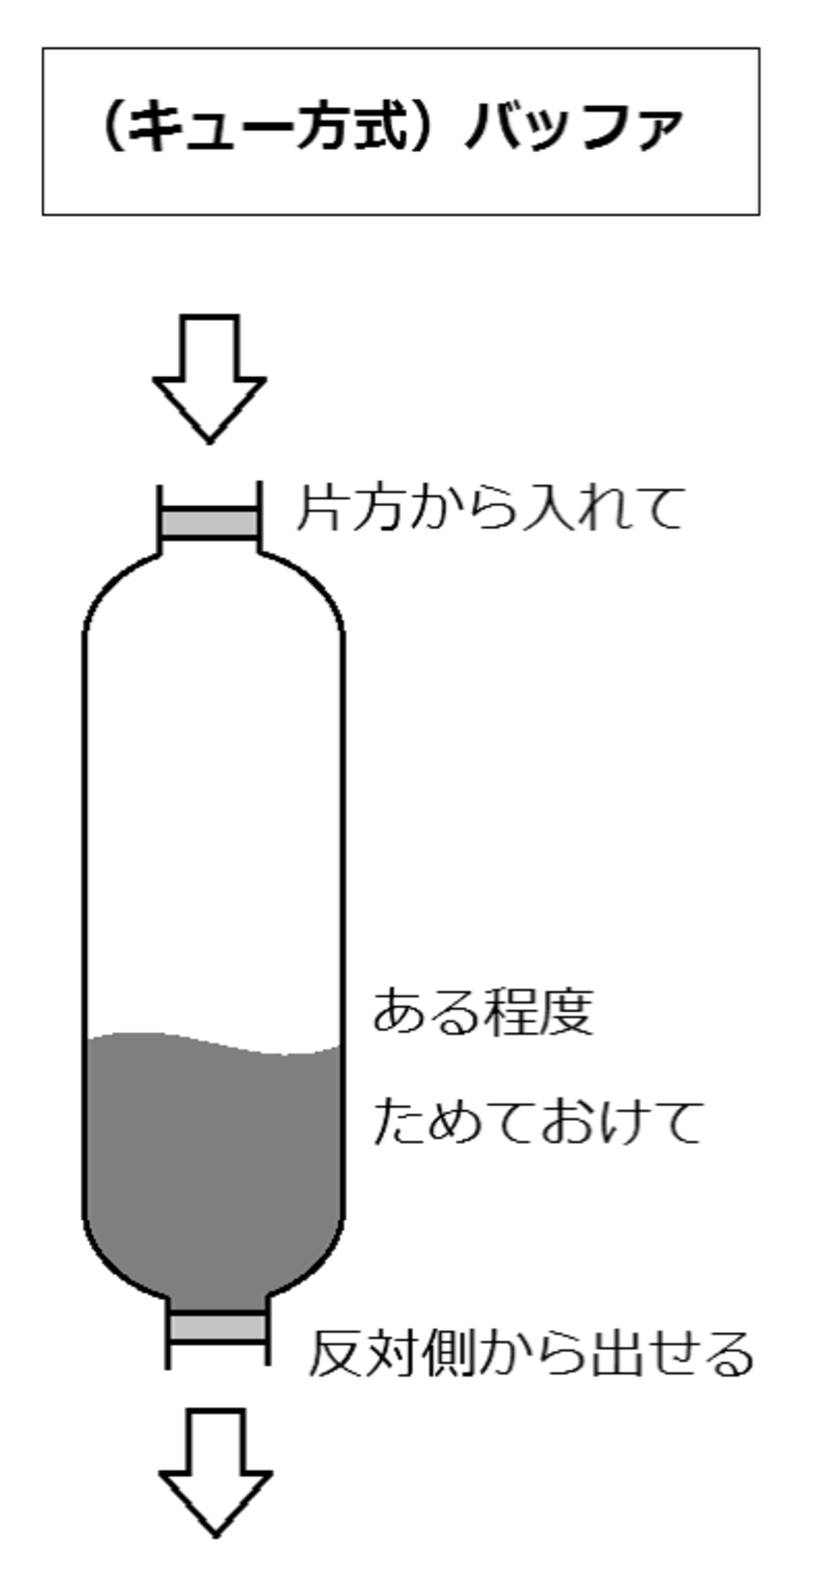
\includegraphics[width=7cm,clip]{res_x_i/model1.eps}
 \end{center}
 \caption{バッファ}
 \label{x_i:model1}
\end{figure}

\answer{僕}{どういうものかはわかったけど……これ何の役に立つの?}

\answer{精}{例えば、上からちょっとずつ入ってくる水をしばらくためてから、一気に下の栓をあけてドバァってやるとか。こういう装置がないとできないですよね。}

\answer{僕}{まあ、そうだけど……。}

\answer{精}{逆に一気に上からドバァって来たのをためておいて、後からちまちま出して使ったり。そういう風に、出し入れの速度を調整するために使えます。}

\answer{僕}{まだ微妙だけど……名前がカッコイイから許した。}

\answer{精}{実際に使われているところを見た方が早いですね。このモデルでは、バッファを縦に二つ、連結します。図をどうぞ。}

\begin{figure}
 \begin{center}
   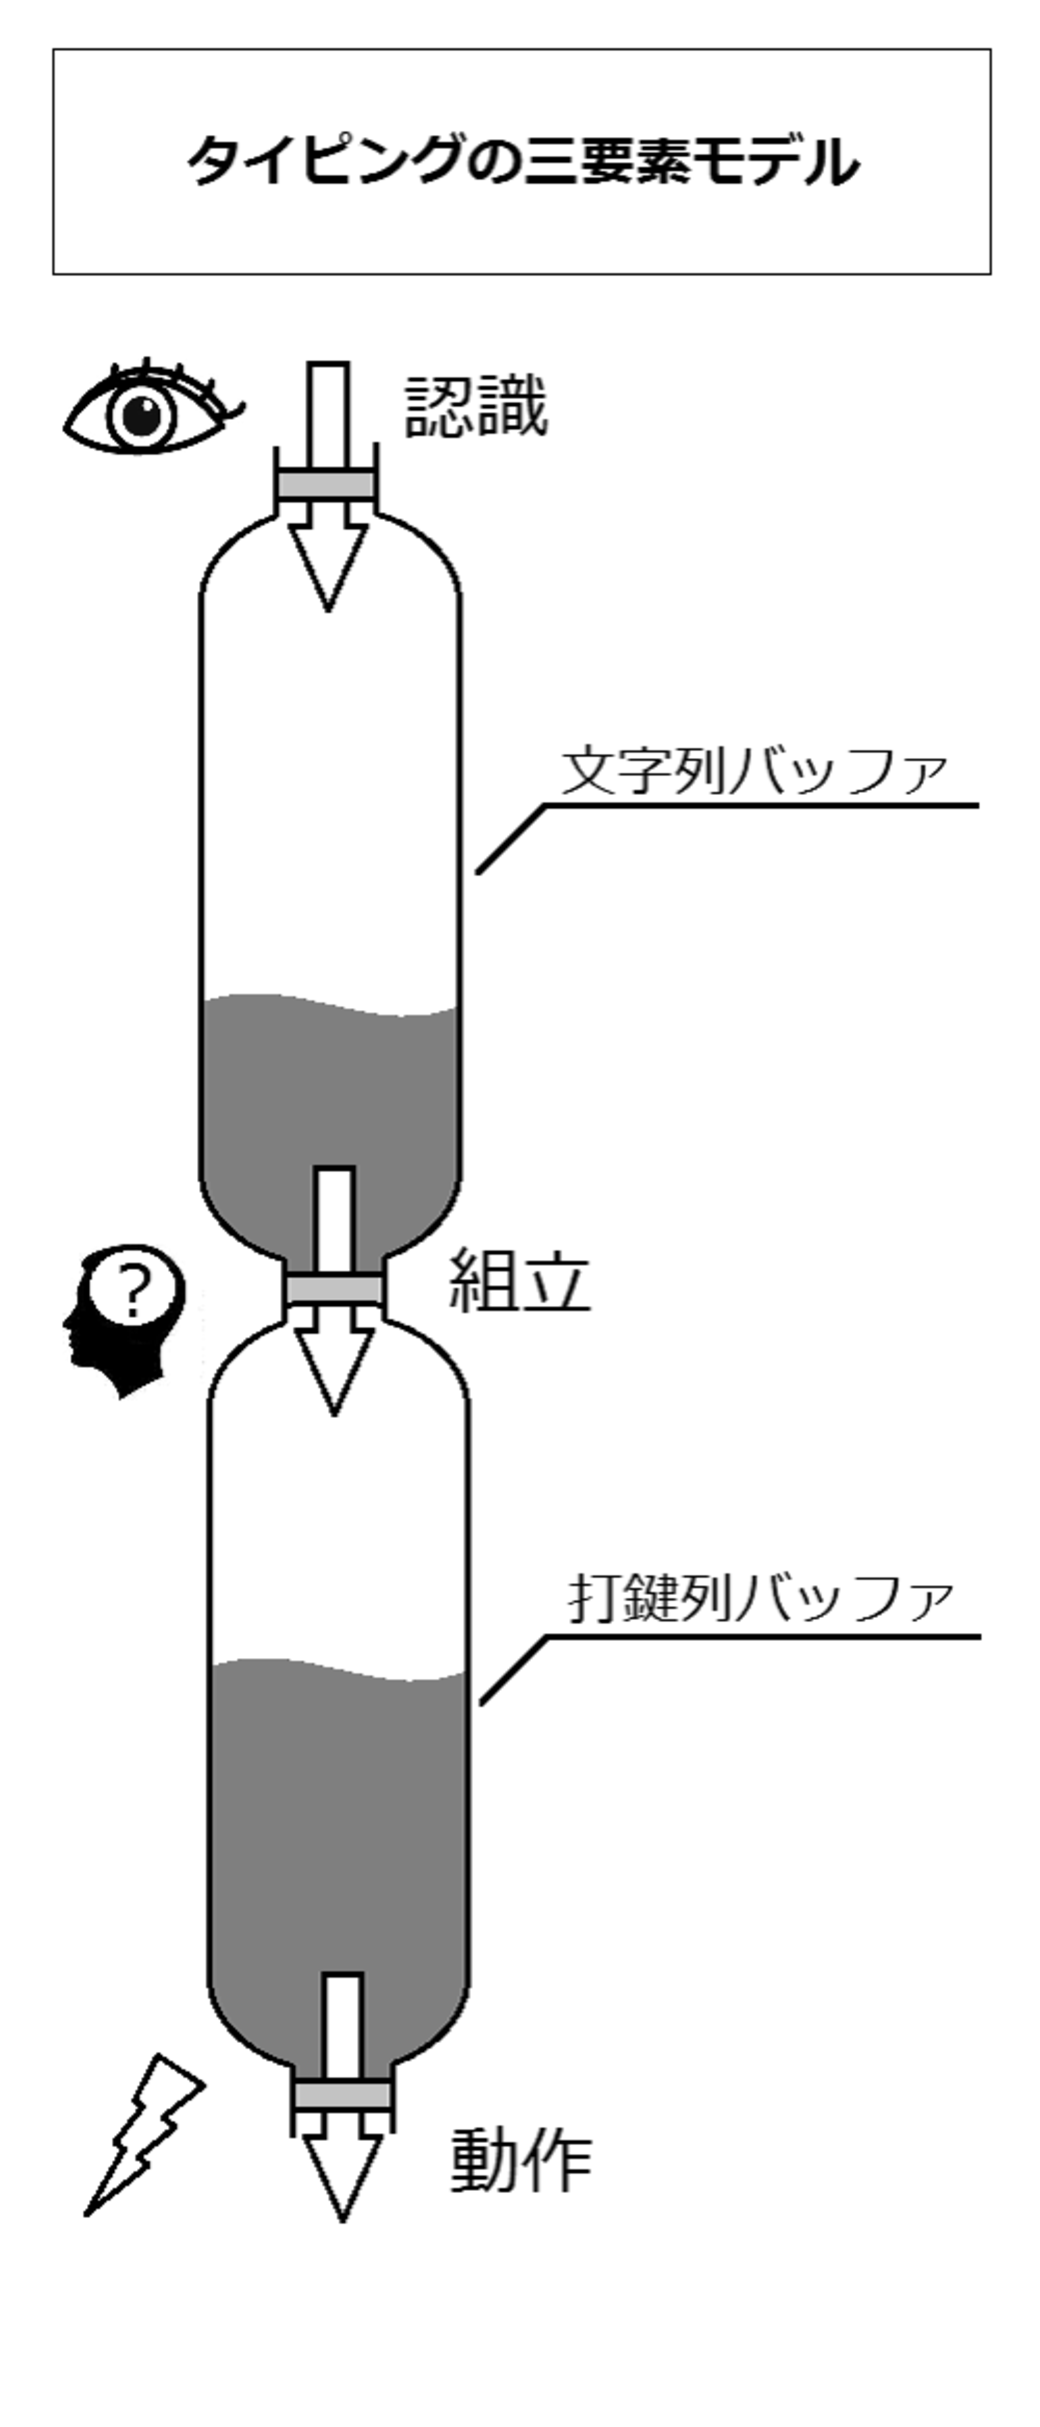
\includegraphics[width=7cm,clip]{res_x_i/model2.eps}
 \end{center}
 \caption{タイピングの三要素モデル}
 \label{x_i:model2}
\end{figure}

\answer{僕}{(連結した!?)}

\answer{精}{図を見てもらえばだいたいわかっちゃうと思いますが……まずワードを「認識」すると、こういう文字列だなという理解が、上の文字列のバッファにたまります。}

\answer{僕}{まだ「文字列」だから、どう打てばいいかってことはイメージできてないわけだね。}

\answer{精}{そうです。「認識」しただけでは打てないので、続けて「組立」です。文字列バッファに溜まっている水(文字列)から一定量取り出して打鍵列を「組立」するわけですね。できた打鍵列が下の打鍵列バッファに溜まります。}

\answer{僕}{おお……。}

\answer{精}{打鍵列が完成したらめでたく「動作」できます。つまり「動作」では打鍵列バッファから水(打鍵列)を取り出して、実際の打鍵を行うことになるわけです。どうですか!}

\answer{僕}{バッファの役割がわかった気がする。}

\answer{精}{大事なポイントとしては、「認識」「組立」「動作」はそれぞれ順番に行われるわけではなくて、同時並行的に進めることができるってことです。}

\answer{僕}{それぞれの栓を同時に水が通過していけるイメージね。}

\answer{精}{そして私たちがやっている競技は、このモデルで言うと、ワードという一定量の水をこの装置の上から注ぎ込んで、どれだけ早く一番下まで\ruby{濾過}{ろか}完了するかという勝負なわけです。}

\answer{僕}{今まで「読む速度が遅い」と言ってたのは「認識」「組立」部分の栓が細いってことで……「打鍵するだけならいくらでも速くできる」って言ってたのは「動作」の部分の栓は他と比べると太いってことだ。}

\answer{精}{考察しやすそうでしょう? e-typing でワードの初めの部分で急ぎすぎるとミスしやすいという話がありましたが、あれは「認識」「組立」が追いついてなくて打鍵列バッファが空なのに、無理に「動作」しようとしたからなんです。}

\answer{僕}{早すぎたんだ……打鍵列が腐ってやがる、と。モデルがあると便利ってこういうことね!}

\answer{精}{これからは、このモデルの理解を前提に話をしますね。}

\subsection{動作がネックになる時}

帰宅後、早速今日得た情報を使って e-typing を攻略しようとしたところ、タイピングの妖精さん(←そういうことで妥協したらしい)に止められてしまった。

\answer{精}{せっかく三要素モデルを紹介したので、「動作」の部分がつらいケースも知って欲しいのですよ。}

\answer{僕}{「動作」は大丈夫だ問題ない、でファイナルアンサーなんじゃなかったっけ。}

\answer{精}{e-typing に取り組む分には、まだしばらくそうです。でも世の中には他の競技種目となるタイピングゲームもあるので。そろそろ他のものも紹介したいと思って。}

\answer{僕}{ぶっちゃけ e-typing のミス音と血しぶきに殺意を感じ始めてたから、嬉しいな。}

\answer{精}{Weather Typing というのが「動作」の限界を感じるには良いので、ダウンロードしてきて下さい。}

\answer{僕}{インストールは僕に任せろー! ……オーケー、あとは WeatherTyping.exe を起動して、と……「シングルプレイ」でいいの? ってか対戦もあるんだね。}

\answer{精}{対戦についてはここでは詳しく解説できないですけど、よく出来ていて楽しいですよ。Weather Typing に慣れてきたらぜひ挑戦してみてください。}

\begin{screen}
Weather Typing\footnotemark

本当はネット対戦がアツくてメインなソフトなのですが、この記事ではシングルプレイに限定した書き方になっています。
対戦にも興味を持たれた方は、上記ページの「その他」→「ロビー」→「参加方法」を参考にロビーに入って常駐するといいでしょう。
ただ最近は常に人がいるという状態ではないようなので、友達を誘うと確実です。
\end{screen}
\footnotetext{\url{http://denasu.com/software/weathertyping.html}}

\begin{figure}
 \begin{center}
   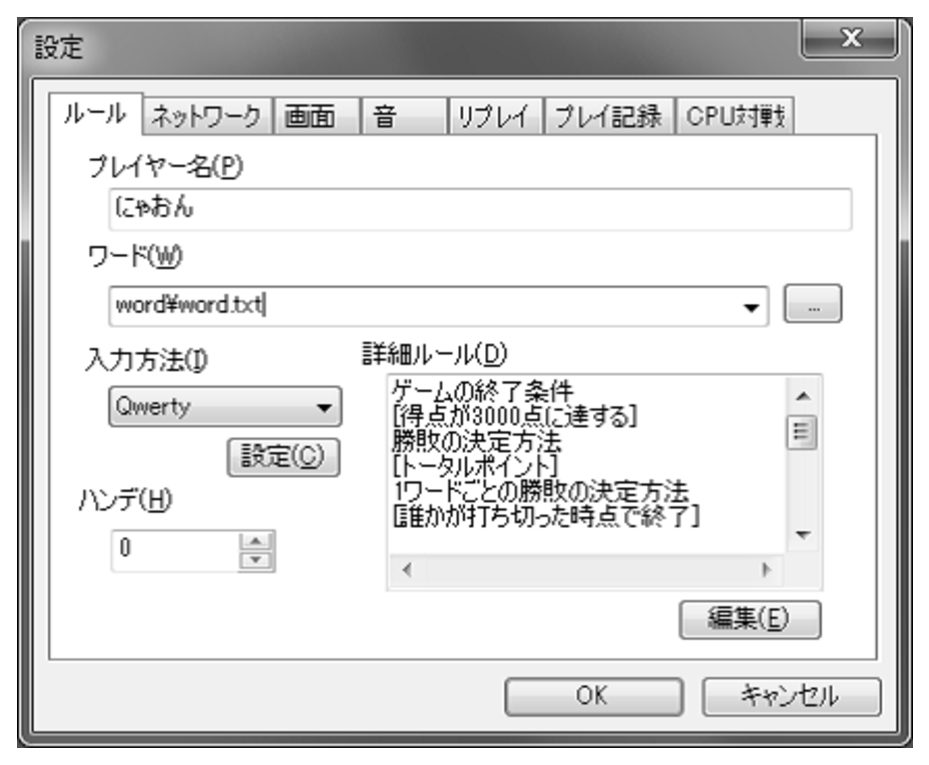
\includegraphics[width=7cm,clip]{res_x_i/wt_setting.eps}
 \end{center}
 \caption{Weather Typing 設定画面}
 \label{x_i:wt_setting}
\end{figure}

\answer{僕}{たくさん設定項目が出てきたけど……。}

\answer{精}{かなり細かく設定ができるんですけど、重要なものはあまり多くないです。今はとりあえず「ワード」とある欄でワードファイルを指定できるということだけ覚えておきましょう。}

\answer{僕}{ワードを自分で作れるんだ。}

\answer{精}{e-typing に慣れていると新鮮ですよね。だから e-typing のワードで練習したいものだけ集めてきて Weather Typing で練習したりなんてこともできます。今はデフォルトのワードファイル word.txt のままでやってみましょう。}

\begin{screen}
独自のワードファイルは直接テキストファイルを編集して作るか、Weather Typing 本体に\ruby{同梱}{どうこん}されている WordMaker.exe を使って作ります。
WordMaker.exe を使えば簡単に作れますので、一度やってみることをおすすめします。
\end{screen}

カタカタカタ。

基本的には e-typing と同種のゲームという感覚だ。画面にワードがひとつずつ表示されて、打ち終わると次のワードに行く。独特のワードに所々つまずきつつも、順調に打つ。……やや長い。

\answer{僕}{……終わった。Complete 30、Speed 510、Accuracy 92 で、Total が 46920。}

\answer{精}{結果の解説は要ります?}

\answer{僕}{いや、もう大体わかる…… Complete はワード数、Speed は e-typing の WPM と同じ意味で、分速何打鍵か。Accuracy は正誤率。Total がスコアでしょ。}

\answer{精}{ばっちりです。ちなみに Total は Speed かける Accuracy で計算されてますよ。}

\answer{僕}{e-typing はスコア計算でミスが三重ペナルティだったから、それに比べるとミスのペナルティは小さいな。}

\answer{精}{Weather Typing の方がスピード重視ですね。ですが、Weather Typing でスコアアタックをする際に一番大切なポイントは、そんな部分じゃないんです。}

\answer{僕}{一番大切なポイント……(ごくり)。}

\answer{精}{Weather Typing では、e-typing の章で解説した初打までの時間「レイテンシ」が、なんと計算に入りません。}

\answer{僕}{計算に入らない? ……ワードが表示されてから、ゆっくり考えて打ってもいいと?}

\answer{精}{イエス。なので、基本的な部分では e-typing に対する攻略が流用できますけど、上級レベルになると e-typing とは別ゲーになります。何しろ短いワードなら最初にじっくり見ておくことで「認識」「組立」を完全に完了できます。つまり打鍵列バッファが満タンの状態で、あとは「動作」だけという所からスタートして競えるわけです。}

\answer{僕}{どれだけ指を速く正確に動かせるかって勝負……。}

\answer{精}{このように打鍵列を十分に組み立ててから一気に打つことを、{\bf ため打ち}と言ったりしますね。}

\answer{僕}{ゲーム的で面白そう。}

\answer{精}{もっと面白くするために、このワードファイルで打ってみるといいです。}

\begin{screen}
ダウンロードして頂けるようにワードファイルを置いておきます。\\
\url{http://dvorak.jp/archive/bura.txt}

Weather Typing のフォルダ内にある word というフォルダの中に保存し、Weather Typing 起動時の画面でこの bura.txt を選択すると使うことができます。

ちなみに、以下の 20 ワードが入っています。

あみあみ かにかに きらきら くいくい\\
くらくら こうこう これこれ さくさく\\
ざわざわ たじたじ ぬくぬく ぬるぬる\\
ふらふら ぶらぶら ぶんぶん ちょこちょこ\\
ぽきぽき むんむん ほげほげ しゅいしゅい
\end{screen}

\answer{僕}{いかにも打ちやすそう……しかも、考えてから打ってもいいと来た。いくらでもスピード出せるでしょ!}

\answer{精}{そう思いますよね。でも実際は……ま、いつものパターンです。}

\answer{僕}{そうわかっていても、突撃するのが僕だった! スタート、っと。}

「くらくら」……えーと\key{K}\key{U}\key{R}\key{A}……楽勝。「さくさく」……楽勝。「ぶんぶん」……人差し指が……。「むんむん」……うーん、きつい。「ざわざわ」……フォオオオ!

\answer{僕}{…… Speed 670。ワードが短いし、レイテンシ無視で考えてから打てるから、さっきより断然速くはなってる。けどワードによっては全然だめだったな。「むんむん」とか。}

\answer{精}{「ぶんぶん」「ぬるぬる」「むんむん」「ぬくぬく」あたりは右手の人差し指を酷使するワードですね。}

\answer{僕}{そいつらはまだいいとして……「ぽきぽき」「ざわざわ」は指がつるかと思った。これが「動作」がボトルネックになる感覚……。}

\answer{精}{その一部ですね。これだけお膳立てすれば「認識」「組立」が十分なレベルでなくても、「動作」もいずれ問題になりそうだということが体感できたでしょ。そして、もっと速くなると e-typing のような競技でも、部分的にボトルネックが「動作」になることはよくあります。}

\answer{僕}{「動作」は物理的な指の動きだから……指を鍛えたりすれば伸ばせるよね。}

\answer{精}{頑張って競技タイピングをやっていると、タイピングに関しては、どんどん指が器用になっていきますね。キビキビと正確に動くようになります。}

\answer{僕}{今までは先読みだとかノーミス意識だとか、脳トレ的な話ばっかりだったけど、筋トレ的な要素もちゃんとあるんだね。}

\answer{精}{タイピングは頭も身体も使う万能競技ですよ。ダイエットにも(多分少しは)なります。}

\answer{僕}{手とか指しか動いてないけど?}

\answer{精}{それでも、二、三時間も本気で打てば汗だくになれます。それくらい激しく「動作」できるくらいに、他の部分が速くなってからの話ですけどね。}

\answer{僕}{タイピングで汗だくは想像したくない……。}

\subsection{打ち分け・最適化}

何度も例のワードファイルで Weather Typing を打っていると、どんどん指の動かし方に慣れてきた。速いワードはとことん速く、遅いワードも詰まらないように。動作部分の訓練は、どうやら僕に向いているらしかった。

\answer{僕}{よし! Speed 750 突破ッ!}

\answer{精}{わあけっこうすごいですねー(←上から目線)。}

レイテンシを無視しているとはいえ、e-typing で 750pt といったらトップレベルだ。これくらいのスピードで e-typing のワードを打ち続けることができれば、750pt ……!

僕はタイピングを始めてから最大級の胸の高鳴りを覚えていた。

だから、こんな挑発をしてしまう。

\answer{僕}{ヨウセイサァン、余裕じゃないっスか……これの記録どんだけなんスかぁ?}

\answer{精}{私ですか?}

\answer{僕}{そっスよ……最初の一回 e-typing 見せてもらってから全然手本見せてくれないじゃないっスか。}

\answer{精}{それは……教育上よくない理由がありまして。でも良い頃合いですね。見せましょう。多分、2000 とか出ますけど。}

\answer{僕}{2000!?}

さすがに冗談だと思った。

―― 二分後 ――

\answer{僕}{ォオオオオオオオオオオオオ!!!}

ワードが爆風に飛ばされるように消えていく……。まさに瞬殺。打ち始めたと思った直後には、すべて打ち終わって、消えている。

そして彼女に乗っ取られた僕の手が、僕の指が、変な方向に曲がって奇妙な動きを見せている。なんだこれは! 大丈夫なのか!? 異次元パワー\ruby{炸裂}{さくれつ}しすぎだろ常考ッ……!?

\begin{screen}
ワードは違います(この動画の方が遥かに高度です)が、参考動画をどうぞ。
ひろりんご氏の独自ワード Speed 1905 Accuracy 100\\
\url{http://youtu.be/jf9kArBHQvE}
\end{screen}

そして打ち終わる。

\answer{精}{……うーん…… Speed 1700 でした。残念、2000 行かなかったですね。まあ「ざわざわ」出すぎでした。運ゲー運ゲー。}

\answer{僕}{ちょ、ちょっと……これは\ruby{卑怯}{ひきょう}っスよ先生……異次元パワー使ってるじゃないスか!}

\answer{精}{はい? ……ああ、手の角度とかの話ですね。}

\answer{僕}{なんなんだこれ……なんなんだこれ……。}

\answer{精}{これが教育上よくない理由そのものです。{\bf 最適化}などと呼ばれています。}

\answer{僕}{やっぱり長門有希的大宇宙能力じゃないっスか!}

\answer{精}{違いますからね……。最適化というのは、ワードに応じて打ちやすいローマ字を選択したり、打ちやすい指で打つように標準の運指を崩したりする技術のことです。前者は{\bf 打ち分け}、後者を{\bf 最適化}として言葉を分ける一派もありますね。}

\answer{僕}{ローマ字を選択? 運指を崩す?}

\answer{精}{えーと……ひとつずつ行きましょう。ローマ字の選択の方の「打ち分け」ですが、これについては e-typing の時に近いことを少しやってます。覚えてませんか?}

\answer{僕}{あれか、水増し打鍵――「う」を \key{W}\key{H}\key{U} で打つみたいな。}

\answer{精}{それそれ。あの時は、打鍵数を増加させるために普通と違う打ち方をするという話でした。今度は、打ちにくいパターンを避けるために使います。}

\answer{僕}{例えば?}

\answer{精}{{\bf C打ち}が代表的なのでこれで解説しましょう。これは「か」「く」「こ」を入力する時に\key{K}ではなく\key{C}を使うテクニックで、打ち分けの一種ですね。}

\answer{僕}{別に\key{K}でも\key{C}でも変わらない気がするけど……。}

\answer{精}{その部分だけ見たらそうです。でも前後のパターンと合わせると……。今回のワードですと「かにかに」「くいくい」「こうこう」「ぬくぬく」「ちょこちょこ」はC打ちによって劇的に打ちやすくなります。}

\answer{僕}{\key{C}\key{A}\key{N}\key{I}、\key{C}\key{U}\key{I}、\key{C}\key{O}\key{U} ……本当に一瞬で打てるような動きに変化した。}

\answer{精}{私は「ちょこちょこ」は CHOCO と打ちますね。速く打つのは、他と比べるとちょっと難しいですけど。}

\answer{僕}{「ぬくぬく」もわからない。\key{C}にしてもあんまり変わらないような。}

\answer{精}{これは運指を崩す方の最適化と合わせて考えないといけないですね。こっちは要するに、このキーはこの指で打ちましょうという原則的なルールを破ることです。}

\answer{僕}{ルールを破る……。}

\answer{精}{そうです。確かにタッチタイプを学ぶ段階ではホームポジションを守り、一般的に教えられる通りにキーごとに担当する指を固定する(標準運指)方が習得が楽でしょう。でもそれって別に、打てるようになった後は破ってもいいですよね。指が動ける範囲はもっと広いので。}

\answer{僕}{タッチタイプってレベルじゃねーぞ! そこまでやるの……恐ろしい……。}

\answer{精}{一例ですが、私は「ぬくぬく」なら\key{N}を人差し指で打った後、\key{U}を中指で打ちます。標準の運指ではないですけど、手の角度的にかなり打ちやすくて自然にいけると思います。そして「く」は右手中指を\key{U}に置いたまま\key{C}\key{U}ですね。こうすると\key{N}\key{C}\key{U}すべて別の指が担当することになって、かなり速いです。}

\answer{僕}{本当だ、\key{U}を中指で打つのは手首をひねる感じで打つと……意外に自然。それでさっきは、手があんな奇妙な動きをしてたのか。}

\answer{精}{そういうことです。今回の他のワードだと「ぬるぬる」「むんむん」「ぶんぶん」にも応用できますね。}

\answer{僕}{「ふらふら」「ぶらぶら」「しゅいしゅい」あたりは?}

\answer{精}{最適化というのは個人個人でやり方に差がありますし、自分でも考えてみるといいんじゃないでしょうか。基本的な方針としては、同じ指を連続して使わないで済むようにすると、たいてい速い運指ができあがります。}

\answer{僕}{「しゅいしゅい」は\key{Y}を左手人差し指で……こうかな? いや、でも「しゅ」\key{S}\key{H}\key{U}にすれば右手で一気に行ける……こっちの方がいいかな……。}

\answer{精}{奥が深いですよね? 最適化に関する議論は、現役タイパーの中でもまったく終わっていないです。各運指を習得するコストや、「組立」の段階で最適化を検討しなければいけないコストを気にして、やらない人もいますし。あまり早い段階からこういう小手先の技ばかりに気を取られるのもどうかと思って、もったいぶってきましたが……今のあなたなら制御できる力でしょう。}

\answer{僕}{うーん(←聞いてない)、「ぽきぽき」はどうやるの?}

\answer{精}{それはもう、左手を右手範囲まで持っていって手伝うんです。}

\answer{僕}{KIMEEEEEEEEEEEE!!!}

\answer{精}{さすがに Weather Typing でこういうワードを打つとき限定ですけどね。他のゲームで出てきたら、普通にぽきぽきした方がいいです。それか \key{P}\key{O}\key{K}\key{I} \finger{9877}。}

\answer{僕}{しかし「ざわざわ」に至ってはもう、どうしようもないね……。}

\answer{精}{(うわーやっぱり最適化ハマっちゃいますか)そういう場合もありますね。}

\answer{僕}{どうしよう?}

\answer{精}{どうもこうも、さっき自分で言っていた通り、指の動きを速くすればいいじゃないですか。最適化の考え方に慣れすぎると、最適化できないパターンは諦めてしまいがちです。でも実は、指を鍛え、運動を洗練させて、打鍵を速くする余地は十分にあるわけです。その基本に立ち返ることも、時には大事ですよ。……と釘を刺しておきますね。}

\answer{僕}{うーん(←全然聞いてない)、ざわざわ……ざわざわ……。}

たかがタイピング、されどタイピング。つくづく底の知れない世界なのだった。

五年後、手を交差させる超絶変態運指「グランドクロス」を完成し、競技タイピング界に大旋風を巻き起こすことになるとは――この時の僕には知る由もない。

\begin{screen}
「精」が釘をさしていますが、他でもない私がそのパターンで長年記録が伸び悩んだ人だったりします。最適化を使うと、ちょっと考え、ちょっと練習すればそのパターンがすぐ速くなるのでハマりがちですね。実際とても楽しいですが、行き詰まりを感じた際には、地道な訓練も大事だと思い出しましょう。

なお、最適化でも対応に困る「ざわざわ」のような文字列をも打ちやすくする、まったく別のアプローチも実はあります。それは、キーボード配列から変えてしまうこと。
一般的には QWERTY と呼ばれる配列でローマ字入力をしますが、タイパーの中には高速打鍵に向くような別の配列を利用して競技に参加している人もいます。ある意味、最適化よりもさらに前衛的なアプローチと言えるでしょう。
詳しくは、配列について詳しく書かれている他の記事を参照してください。
\end{screen}

\section{タイプウェルの登竜門}
\begin{screen}
無能! 死ね!\\
―― dqmaniac, 己の打鍵失敗に憤って
\end{screen}

\subsection{国内最強ランキング}

タイピングのモデルを知り、最適化や打ち分けを知り、自分で攻略法を考えながら打ち込むことができるようになって以来、タイピングに対する情熱はますます燃え上がった。練習量は倍になり、スキマ時間に最適化について考えるようになり、授業中など暇さえあれば指のストレッチをする。

当然の結果として、成長もすさまじかった。e-typing で 500pt の壁を打ち破るとほぼ同時に Weather Typing の word1 で Lv6 (60000 点)到達。最適化練習のワードでは Speed 1400 が安定して出せる。

e-typing 腕試しのランキング 1 ページ目に自分の名前が載っているのを見てはニヤつく毎日――そんなある日のことだった。

\answer{僕}{この「タイプウェル」っていうのは……なんだろ?}

e-typing のランキングに、その名前を見つけてしまう。

\answer{精}{みつ……けて……しまったん……ですね……。}

おどろおどろしい声色を響かせながらキーボードからお人形的上半身が生えてくる。もちろん、今更驚きはしない。

\answer{僕}{ちょっと待ってよ。まだ隠し事があったの?}

\answer{精}{紙面……構成の……都合……。}

\answer{僕}{なんでもいいけど、そのテンションやめよう、つまんないんで。}

\answer{精}{はーい(←キーボードから飛び出た)。タイプウェルというのは国内で最もレベルの高いランキングを持つ競技タイピングソフトです。現代でも最もメジャーな競技ソフトと言ってもいいでしょう。}

\answer{僕}{国内で最もレベルが高い!? e-typing が最大最強って言ってた気がしまくりんぐですが。}

\answer{精}{日常的な参加者数では、e-typing ですよ。でもタイプウェルのランキングサイト GANGAS では、もう 10 年以上にもわたって記録が蓄積されているんです。e-typing のようなリセットはありません。}

\answer{僕}{10 年……だと……。}

\answer{精}{それも、GANGAS に登録されるのはその人の最高記録。色々なタイパーが――あらゆるタイピング界の偉人が、かつてトップだったタイパーが、伸び盛りの現役勢が――何年もの年月を積み重ね到達点として出した、至高の最高記録! それが何百・何千と集められているこのロマン! わかりますか!?}

\answer{僕}{わかりますッッ!!!}

\answer{精}{よろしい! 突撃です!! 大海があなたを待っている!!!}

\begin{screen}
GANGAS - Type Well Fan\\
\url{http://www.twfan.com/}

本体の入手はページ下部の「概要・ダウンロード」からどうぞ。
\end{screen}

\answer{僕}{僕のブラウザが火を噴いた!}

\answer{精}{タイプウェルの文化はそれだけでかなり深いものがあるので、ページを一見しただけでは何がどうなっているのかわからないですよね。}

\answer{僕}{なんか盛り上がってるということはわかる……「国語R」「国語K」「英単語」「オリジナル」っていうのが種目の名前かな?}

\answer{精}{そこから説明するのがよさそうですね。実はそれらは、それぞれ別のソフトです。}

\answer{僕}{同じタイプウェルなのに?}

\answer{精}{exe ファイルが別、と言えばわかりますかね? ひとつのソフトに全部の種目が入っているんじゃなくて、それぞれ別のソフトになっています。「国語R」はローマ字入力で日本語を打つソフト、「英単語」は英単語を打つソフト、「オリジナル」はランダムな数字みたいな、日本語でも英語でもないような独特のワードを打つソフトです。}

\answer{僕}{「国語K」は?}

\answer{精}{ローマ字入力ではなくて、かな入力で日本語を打つソフトですね。今あなたが打っている QWERTY 配列を使ううちは、お世話になることはないです。}

\answer{僕}{じゃ、とりあえず 3 つをやればいいんだ。}

\answer{精}{ところが、これらのソフトそれぞれに 4 つのモードがあります。}

国語 R
\begin{itemize}
 \item 基本常用語 (常用)
 \item カタカナ語
 \item 漢字
 \item 慣用句・ことわざ(慣こと)
\end{itemize}

英単語
\begin{itemize}
 \item 基本英単語 1500(基本)
 \item 拡張基本英単語 A-F(A-F)
 \item 拡張基本英単語 G-P(G-P)
 \item 拡張基本英単語 Q-Z(Q-Z)
\end{itemize}

オリジナル
\begin{itemize}
 \item 小(大)文字のみ(のみ)
 \item 大文字小文字混在(混在)
 \item すべてのキー(すべキー)
 \item 数字
\end{itemize}

\answer{僕}{圧倒的なボリューム! これ全部別のゲームってこと?}

\answer{精}{ソフトによって打鍵数や表示形式など、細かな点が違ったりはしますが……基本的にはワードが違うものがこれだけある、って認識でオーケーです。}

\answer{僕}{ワードは e-typing みたいに週で変わったりはしないんだよね。}

\answer{精}{本体のバージョンアップで若干の追加・削除が行われたりはしましたが、基本的に変わりません。同じワードが過去から現在に至るまで打ち込まれてきたということです。}

\answer{僕}{燃えてきたよぅ……説明聞いてる場合じゃねぇ!}

\answer{精}{(こんな性格だったっけ……)}

自信があるのはもちろん今まで練習を重ねてきたローマ字日本語入力。タイプウェル国語Rをダウンロード、解凍、そして速攻実行。

\answer{僕}{行くぜ! ……ってあれ、詰まった。なにこれ。}

\answer{精}{ワードとワードの区切りで \key{Space} を押さないといけないんです。}

\answer{僕}{そういうのもあるのか! 任せて!}

カタカタカタカタ……。

\answer{僕}{先生出ました! ダブルエス!! レベル SS 出ました!!!}

\answer{精}{おめでとうございまーす。}

\answer{僕}{はぁ……はぁ……これ疲労すごいよ。長いし……ずっと打ちっぱなしじゃん。}

\answer{精}{e-typing や Weather Typing とは毛色の違う競技ですね。レベルやランキングがタイムだけで決まる点も異色です。ミス数とか関係ありません。とにかく速さ命! っていう、とんがった競技ですね。}

\answer{僕}{ミス 30 もあるけど……初っ端から SS 来たんで、賢者モードぉ。}

\answer{精}{……現実を突きつけるようで申し訳ないですけど、タイプウェルのレベルは基本的にこれだけあります。大区分として無印・S・X・Z があって、それぞれの中に J-A のような小区分がある、と読み取ります。}

\begin{figure}
 \begin{center}
   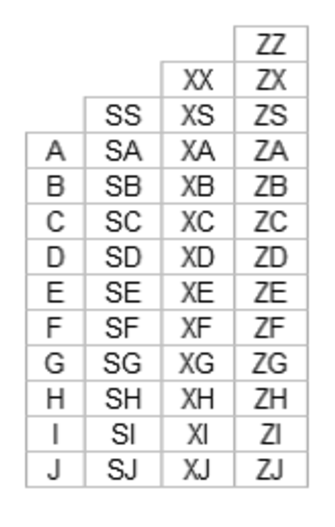
\includegraphics[width=5cm,clip]{res_x_i/tw0.eps}
 \end{center}
 \caption{レベル一覧}
 \label{x_i:tw_level}
\end{figure}

\answer{僕}{僕は SS だから……中間程度!? e-typing 1 ページ目常連のこの僕が!?}

\answer{精}{スペースを押すのにも慣れていない状態で初見常用 SS なら、それなりだと思いますよ。慣れたら X の半ばから X の上の方くらいまではすぐ行けると思います。}

\answer{僕}{XE とかってこと? それってレベル的にどうなの?}

\answer{精}{どこに出しても恥ずかしくないタイパーだと思います。ただ、上には上がいる世界なので……さっきの GANGAS のページからランキングを見てみるといいんじゃないでしょうか。}

\answer{僕}{Z ばっかりじゃん……どこだよ、どこだよ XE ……オウフ、一番下ですか……1000 位とか……。}

\answer{精}{今の記録と比べるなら、SS というと 50 秒以上かかってますから……トップレベルの人は倍以上速く打っていますね。}

\answer{僕}{レベル高すぎワロエナイ。}

\answer{精}{同じワードを何年も打ち込んだりしているわけですしね。打ち切り回数(最後まで打ってタイムを出した回数)も千とか万とかの世界です。e-typing のようなペラペラのランキングとは違うんですよ。10 年積もり積もった結果ですから。日々ランキングを励みにコツコツ記録を伸ばしていって、いつかは憧れの 50 位以内(一番上の枠)に……! と、こういうスタンスで見るものです。}

\answer{僕}{やる気はあるつもりだったけど、ちょっと気が遠くなるかも……。}

\answer{精}{まだまだ伸び盛りですし、心配は要りません。今の自分のレベルより一つ上を目指し、もう一つ上を目指し……とやっている間に、いつの間にか成長しているものです。}

\answer{僕}{ステージをひとつずつクリアしていくって感じなのね。}

\answer{精}{まさにそれです。ランキングに関して、ちょっとモチベーションになりそうなことも言いましょうか? 国内にはこれ以上ハイレベルなランキングは存在しないので、ここで 100 位になれば、かなり堂々と全国 100 位を自負できます。というか国内歴代 100 位ということなので、現役タイパーの中でなら間違いなく 100 位以内と言えるでしょう。}

\answer{僕}{それは嬉しいな。}

\answer{精}{ちなみに、各ソフトのランキングは「総合ポイント」という得点のようなもので競われています。}

\answer{僕}{何がポイントになるわけ?}

\answer{精}{4 つある各モードの自己最高記録のタイムです。まず各モードごとに、タイムに応じたポイントが計算されて、その総和がそのソフトの「総合ポイント」です。}

\answer{僕}{最高記録以外はポイントにはならないのか。}

\answer{精}{ちょっと極端ですよね。でも、だからこそ自己最高記録をどんどん伸ばそうと必死になるわけです。}

\answer{僕}{みんな、こんなに頻繁に自己最高記録を更新してるってこと?}

\answer{精}{そうです。現役競技者のハングリーさはものすごいですよ。ぜひ影響を受けて、少しずつでも記録を伸ばせるようがんばってみてください。}

\answer{僕}{まだわからない部分が多いけど……とりあえず打ってみて、ランキングに参加していればいいんだね。}

\answer{精}{まずはカンペキでしょう。……ランキングについては、本当はもっと色々紹介したいですが……自分で見て回って色々感じて欲しいので、この辺にしておきますね。}

\begin{screen}
なおランキングの参加方法ですが、各タイプウェルの中から記録がコピーできるので、それをメールで送ると、毎週土曜日に反映されます。即時反映でない点も面白いところです。目立った更新だった場合はトップページで紹介されることも。

参加方法について詳しくは、GANGAS 公式の解説\footnotemark を熟読してください。
\end{screen}
\footnotetext{\url{http://members.jcom.home.ne.jp/gangas2/entry.html}}

\subsection{使い方}

全タイプウェルをせっせとインストールした僕。わざわざ全部インストールしたのを見届けた後に、あっけらかんと彼女はこう言う。

\answer{精}{タイプウェルは基本 4 種類あるという話をしましたけど、今からは国語Rに限定して話を進めます。}

\answer{僕}{OH!? タイプウェルオリジナルという謎のソフトに心惹かれてるんだけど?}

\answer{精}{タイプウェルの活用の仕方を身につけて欲しいと思うんですけど、国語、英単語、オリジナルそれぞれ仕様が違って面倒なんです。それに、英単語やオリジナルは e-typing や国語 R とはワードが全然違って、完全に別の競技です。今の段階で手を出すのは早すぎますね。英単語やオリジナルもオールラウンドに打てれば、それはすごいですけど……まずは国語Rに専念してタイプウェルという文化そのものに慣れるのをおすすめします。}

\answer{僕}{うー……了解しておくけどさ。}

\answer{精}{まあ、細かい点が違うだけなので、まず国語Rをおさえておけば大丈夫です。応用が利きます。これがタイプウェル国語Rの基本画面ですね。}

\begin{figure}
 \begin{center}
   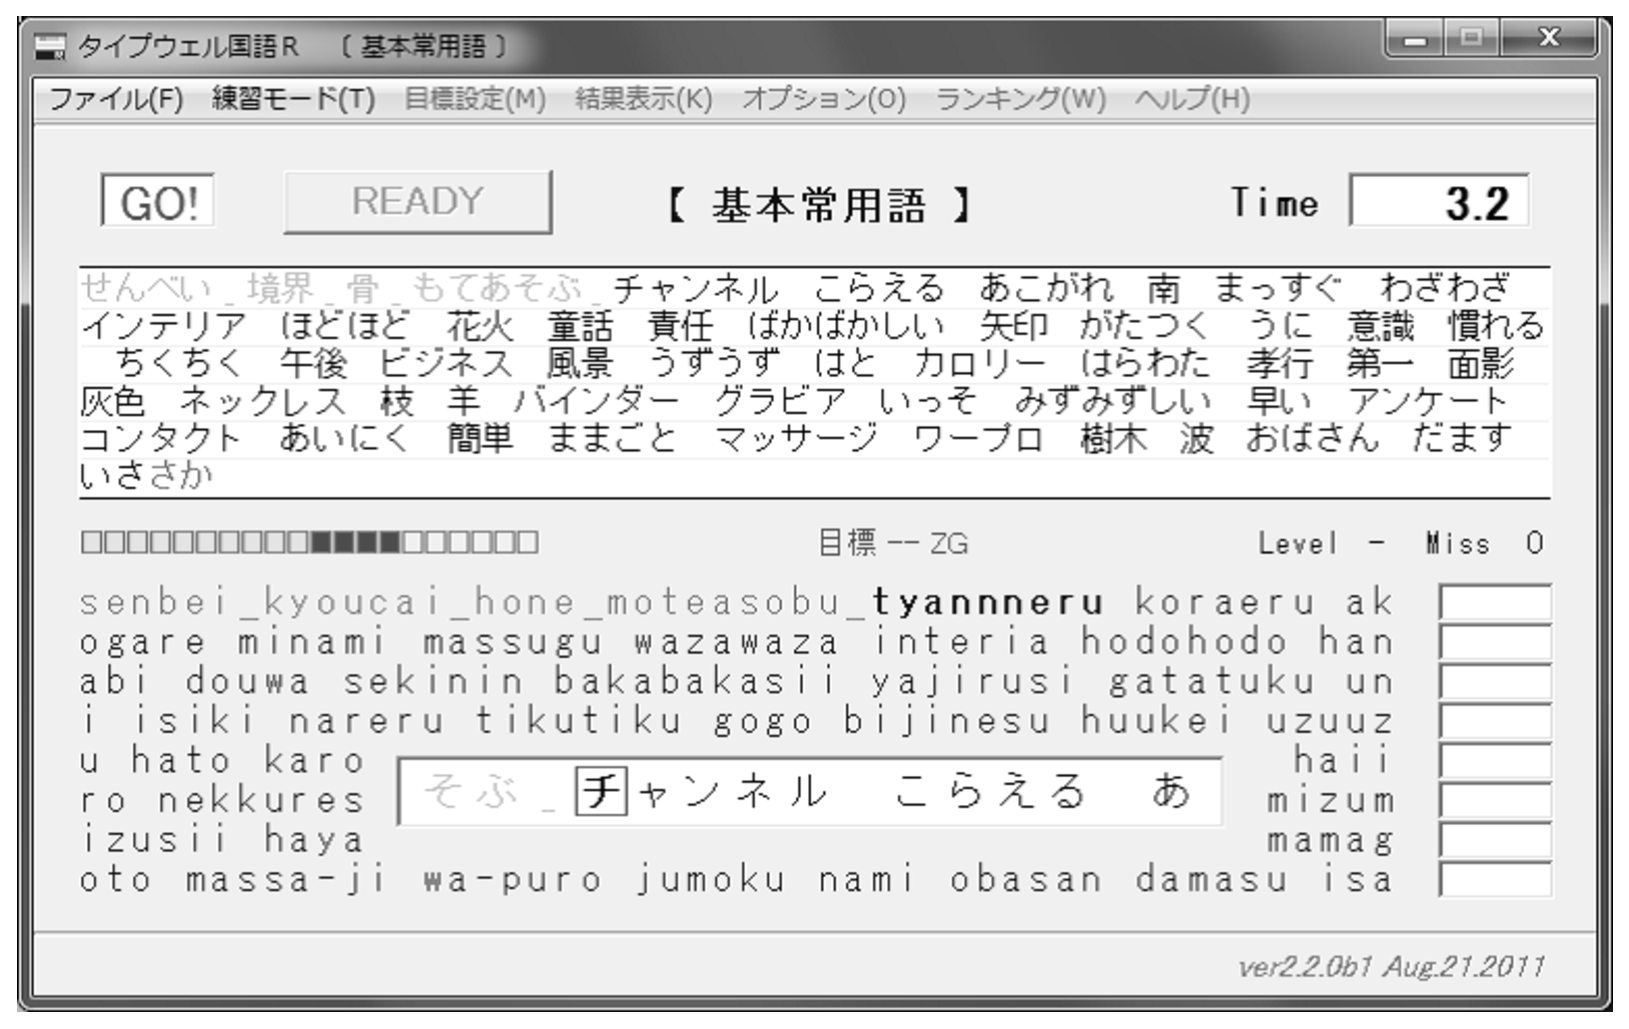
\includegraphics[width=7cm,clip]{res_x_i/tw1.eps}
 \end{center}
 \caption{タイプウェル国語R}
 \label{x_i:tw_mainwin}
\end{figure}

\answer{僕}{機能が詰まってる感じがするよね。}

\answer{精}{言い出せば本当に色々な機能があるんですが、全部解説して、活用法を書き出すとこれだけで本が一冊できちゃうので、タイプウェルプレイヤーなら絶対におさえておきたいポイントを見ていきましょう。}

\subsubsection{基本}

\answer{僕}{この READY っていうボタンをクリックでスタートして……とかそんなことはわかってるから。情強勢甘く見ないでね。}

\answer{精}{いえ、クリックする人は完全に情弱で、普通\key{Space}キーを使います。\key{Enter}でもいいですけど、手をホームポジションに自然に置いたまま、\key{Space}でスタートするのがベターでしょう。}

\answer{僕}{あーそっか。でも e-typing もスペースでスタートだったから、慣れてる。}

\answer{精}{\key{Esc} で中断できるのも e-typing と同じですね。これはある意味一番重要な機能かもです。}

\answer{僕}{……わお、本当に一瞬で中断できる。良い感じに打てるまで何度もこれでやり直せばいいと。}

\answer{精}{そういうスタンスもありますけど、はじめは毎回打ち切る(中断しないで最後まで打つ)ことをオススメします。タイプウェルの特徴のひとつに、記録が色んな面で蓄積されるという点があるんです。だからダメな記録でも、打ち切って蓄積すると……後から嬉しいかもしれません。}

\answer{僕}{他には?}

\answer{精}{先ほども説明しましたけど、各ワードの間に空白が挟まって出題されます。この空白部分では\key{Space}を毎回押さなきゃいけません。}

\answer{僕}{慣れないなぁ、これ……。}

\answer{精}{誰でも最初はそう思うんですけど、慣れてくると親指で\key{Space}を打つのはほぼ完全に無意識になります。なので最初ちょっとイラッとしても、そこは我慢です。我慢して慣れるだけの価値がタイプウェルにはあります、絶対。}

\answer{僕}{右親指で打つか、左親指で打つかは、どっちでもいいわけ?}

\answer{精}{さすが、良いところに気がつきますね。ですが、どちらで打つ人もいて、どちらが有利という結論なんてのは出ていないです。なので、どっちでも良い感じなのですが……ただ、後から変えるのはかなり大変なので、自分で納得した方で打つようにしてください。}

\answer{僕}{そんなこと言われても、余計困るよ。}

\answer{精}{うーん、完全に個人的な意見でよければ、左を薦めます。右手は\key{N}\key{M}周りでの最適化があったり、\key{-}\key{p}など遠目のキーが多かったりするので、左親指を使う方がわずかに有利なんじゃないかと。最適化をしない標準運指スタイルですと、また違ってくるんですけど。また、多くの人は右利きなので、右で打つ方がいいのではという意見もあります。結局、合う・合わないで決めるしかないでしょうね。}

\answer{僕}{うーん……。}

普段のタイピングでも左親指を使っていた僕は、少し悩んだあと、やはり左で打つことに決めた。こういうのは勢いだ。

\answer{精}{ゲームとしての操作方法は、これだけですね。シンプルです。}

\subsubsection{設定}

\answer{僕}{メニューバーに大量に項目があるけど……。}

\answer{精}{ほぼすべての機能がそこから呼び出せるようになっています。タイパーはキーボードが好きなので、慣れてくるとキーボードショートカットを使うはずですけど……慣れてないうちはメニューを開いて、見て回るといいですね。そこにショートカットキーも載っているので、見ているうちに覚えます。}

\answer{僕}{大体どういう機能があるのかも、見ればわかるね。}

\answer{精}{本当に重要な部分だけ見てみましょう。「練習モード」は 4 つあると説明したモードの切り替えですね。}

\answer{僕}{それぞれワードが違う、と。}

\answer{精}{記録もモード別にまったく別に集計されます。当たり前ですけど。「カタカナ語」「漢字」「慣用句・ことわざ」はそれぞれ難易度が高いので、慣れないうちは「基本常用語」一本でいいでしょう。文字通り、基本ですから。慣れてきたら総合成績を意識して、それぞれ攻略してみると面白いです。}

\answer{僕}{「目標設定」は?}

\answer{精}{目標を設定すると、プレイ画面にあるゲージ(インジケーター)で今の記録の目安をリアルタイムに確認できるんです。}

\answer{僕}{それはぜひ詳しく。}

\answer{精}{目標より速いペースか、遅いペースかが、インジケーターの表示になります。速いと青ランプが、遅いと黄・赤のランプが増えていきます。詳しい動作は、実際にプレイして確認した方がいいですね。}

\answer{僕}{まず、目標で高いレベルが設定できないんだけど……。}

\answer{精}{そこもポイントで、今出ている最高記録のレベルよりひとつ上までしか目標に設定できないんです。}

\answer{僕}{ああ、新しいレベルを出すと次のステージが解放されるんだね。レベルをひとつずつクリアしていくって、こういうわけか。}

\answer{精}{そうです。はじめはポンポンと自己最高記録が出せると思うので、まずはどこまで行けるかトライしてみるといいですね。ちなみにゲージの速度は「オプション」内の「目標インジケーター設定」で変更可能です。埋もれてますけど、これは大事な設定項目ですね。}

\answer{僕}{速く動くようにしておけばいいかな?}

\answer{精}{人によって好みがありますね。速く動きすぎると、そこに目が行ってしまって集中できないという人がいます。そういう人は遅くしたりしますし。}

\answer{僕}{他のオプションは弄らなくていいの?}

\answer{精}{インジケーターに比べると重要度は落ちます。お好みでどうぞ。}

\begin{screen}
「画面サイズ」は大きい方が文字が認識しやすくて良い、「カウントダウン設定」は「すぐにスタート」じゃないとイライラする、ミスの音はいらない、などなど、人によって色々な好み・こだわりはあります。
タイプウェルは本格的に取り組むと年単位でお世話になるので、プレイしているうちに勝手にそういうこだわりが出てきます。
\end{screen}

\subsubsection{結果表示}

\begin{figure*}
 \begin{center}
   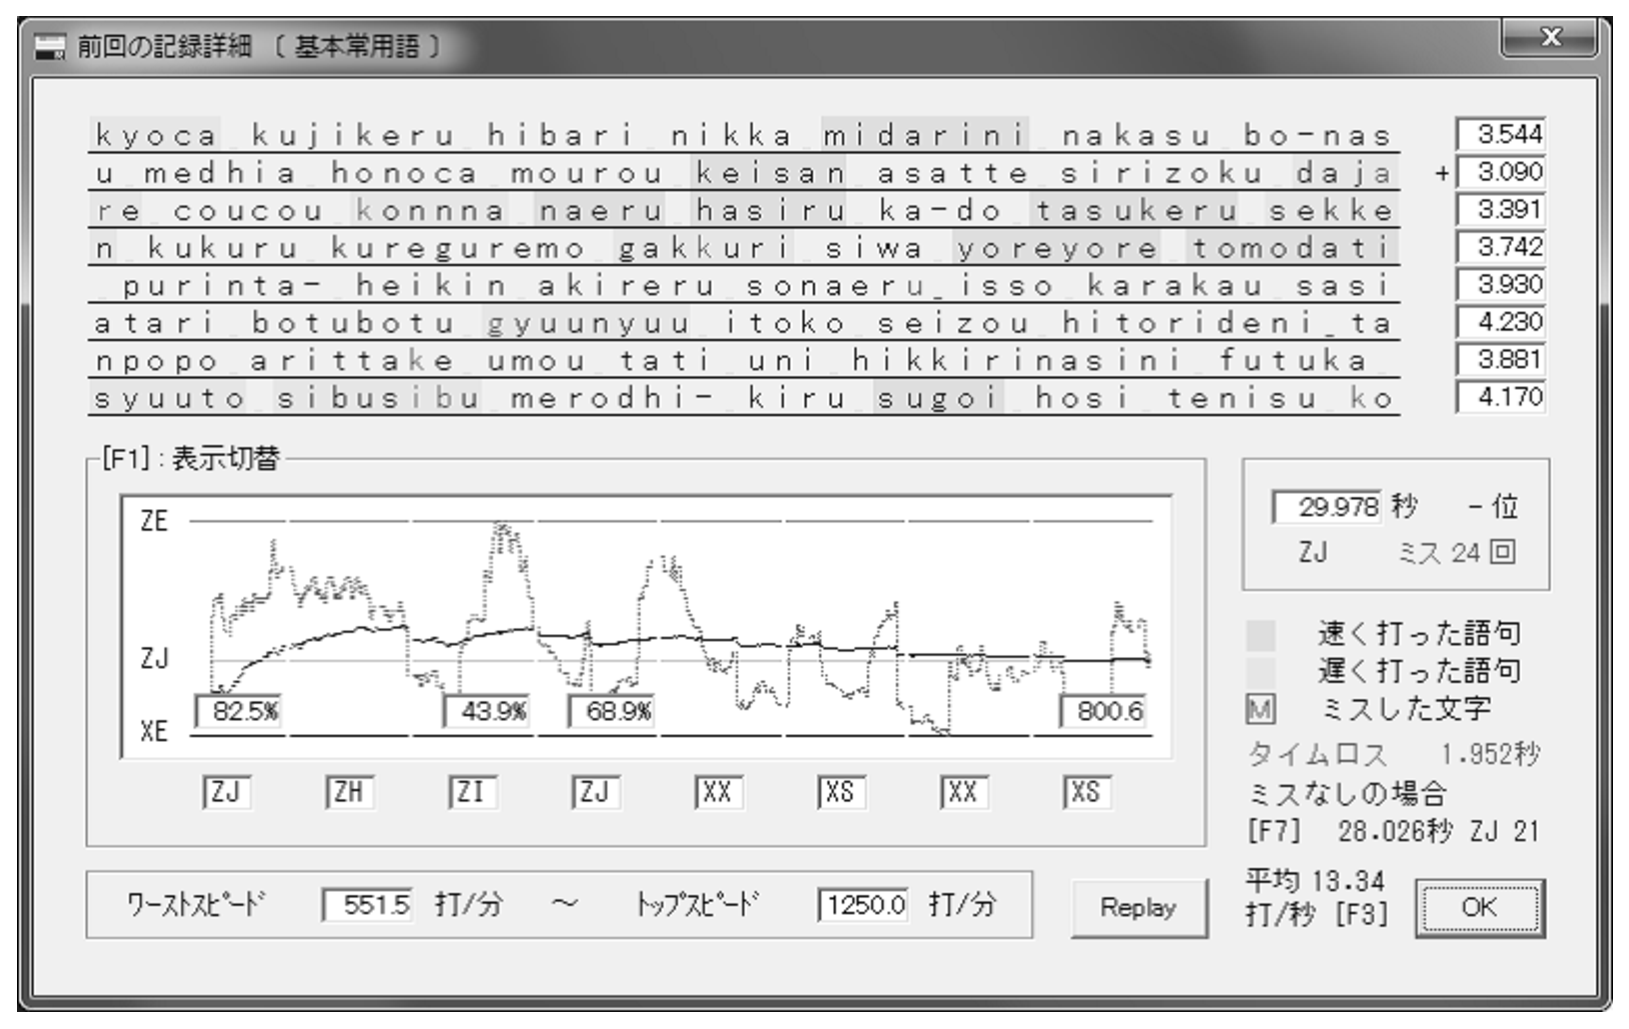
\includegraphics[width=14cm,clip]{res_x_i/tw2.eps}
 \end{center}
 \caption{記録詳細画面}
 \label{x_i:tw_record}
\end{figure*}

\answer{精}{最後まで打ち切ると、こういう画面が出ると思います。「記録詳細」画面ですね。}

\answer{僕}{似たのは出るけど……こんなグラフみたいなのは表示されてないよ。}

\answer{精}{その画面で \key{F1}を何度か押してみてください。押す度に表示が切り替わります。そのうちの一つの表示モードがこのグラフ表示ですね。一番情報量が多いので、玄人はこの表示モードで見ることが多いです。}

\answer{僕}{っていうか超速い記録じゃんこれ! Z とか出てる。}

\answer{精}{私がそれなりに真剣に打つとこんな感じですね。見方はわかります?}

\answer{僕}{わ、わかるよ。……と言いたいとこだけど、よくわからないのもある。}

\answer{精}{打ち切りタイムとか、この打ち切りのレベルとか、ミス回数とかは大丈夫でしょう。}

\answer{僕}{その上に並んでる数字は?}

\answer{精}{「ラップタイム」と呼ばれています。国語Rは400打鍵のタイムを競いますが、それを8のラップに分けて考えることがあります。}

\answer{僕}{各ラップ 50 打鍵……この画面のアルファベットの一行分がラップなんだね。ちょうど 8 行あるから。}

\answer{精}{そういうこと。こうやって分割することで、序盤で速かったけど後半が遅くなった、なんていう大体のプレイ結果を考えやすくしてあるんです。ちなみに各ラップのことを 1 ラップ目、2 ラップ目、なんて呼びますね。}

\answer{僕}{この例だと、3 秒で打っているラップもあれば、4 秒以上かかっているラップもあるね。}

\answer{精}{ラップごとにレベルも表示されていますね。グラフの下にレベルが並んでいるのがそれです。そしてこのグラフでは、もっと細かくスピードの推移を見ることができます。グラフ上の好きな位置にカーソルを合わせると、その地点が上の打鍵内容のどこにあたるのか、またその瞬間の速度はどれくらいだったのか、調べることができるんですよ。}

\answer{僕}{一番スピードが速かった瞬間は…… 3 ラップ目の中盤「萎える」「走る」のあたりか。本当に詳細だ。}

\answer{精}{一番速かったところの速度を「トップスピード」、遅かったところの速度を「ワーストスピード」と呼んでいます。下の方にそれぞれ分速何打のペースか、出てますよね。}

\answer{僕}{一番遅いところでも 551.5……僕の e-typing よりずっと速いってことか。}

\answer{精}{\key{Space}も打鍵にカウントしていますし、ワードごとの小休止なしでずっと続けて打ちますから、e-typing と単純に比較はできないですけど……大体のペースのイメージは湧きますよね。Weather Typing で一瞬だけ高速に打つ練習もしましたから、トップスピード 1250 打/分がどれくらい速いのかも想像がつくんじゃないでしょうか。}

\answer{僕}{「萎える」は\key{U}を中指でっていう最適化を使えば一瞬で打てそうだもんね。}

\answer{精}{e-typing でもやった先読みも駆使して、今打っているワードの次の単語・次の次の単語くらいまでは認識できてますから、組立が間に合えば最適化も使えますね。ワードの種類もそんなに多くない(各モード 2000 程度)ので、ワード慣れもできますし。}

\answer{僕}{今までやってきたことをすべて駆使して挑む……燃えざるを得ないシチュだよ、これは。}

\answer{精}{慣れれば慣れるほど面白いですよ。打つだけでどんどん伸びる時期はそれでいいですけど、伸び悩んできたらこの記録詳細画面で自分の打鍵をよくチェックして、改善点を探したりするといいです。}

\answer{僕}{他にも色々結果を見れる画面があるんだよね?}

\answer{精}{他はいくつもの結果を一覧したり、最高記録を並べたりする画面ですね。個々のプレイの詳細じゃなくて、統計的にどうなのかを見たい時に使います。ショートカットキーが \key{F5}\key{F6}\key{F7} と集中しているので、その辺ポチポチ押してみるといいです。}

\begin{screen}
具体的には、次のような画面です。

\begin{itemize}
 \item トップ15 (\key{F5}):そのモードの自己15位までの記録を一覧。トップスピードやワーストスピードのランキングも。
 \item カナ別成績:各カナごとにかかった平均時間を一覧。
 \item 総合成績(\key{F6}):各モードの最高成績を並べて見られるほか、オンラインランキングで競うことになる総合ポイントが参照できる。
 \item 練習実績(\key{F7}):日々の練習回数、その日の最高タイムなどが参照できる。
\end{itemize}
\end{screen}

\subsection{攻略法?}

単語の間にスペースを挟むのに苦労しながらも何度か打つと、XI が出て、続けて XH が出て……次々に上のランクを出すことができた。

\answer{僕}{XG 出たよ! エーックス! ジー!}

\answer{精}{おめでとうございます。私の予言通りですね。XD くらいまではこのまま行けちゃうと思いますよ。}

\answer{僕}{いつもみたいに、その先へ行くための攻略法も教えてよ。XD なんてすぐ行くから、XA とか ZJ とかのレベルを目指す方法をさ。}

\answer{精}{行き詰まってから言われないとわからないですよー。}

\answer{僕}{もったいぶらないでいいじゃん、もう隠すことなんてないでしょ。}

\answer{精}{それはないですけど……どちらかというと逆で、「これが攻略法だ」って自信満々に教えることができるようなことって、もうそんなにないんですよ。今まで教えて来たようなことをタイプウェルに応用していくだけなんですから。}

\answer{僕}{でも行き詰まったら教えてくれるんでしょ?}

\answer{精}{うーん、つまり、個人差があるのですよ。実際に行き詰まったあなたを見たら、私はきっと「ここが悪い」「ここを改善しよう」ってアドバイスできます。でも今の段階じゃ、あなたがどういうスタイルになって、どこで伸び悩むかなんて、全然わからないわけで。}

\answer{僕}{誰にでも言えるような「攻略法」はない?}

\answer{精}{「スムーズに詰まらず打ちましょう」「速く打てるワードを速く打ちましょう」みたいな中身のないことは言えますよ? でも、実際にどうやって進んでいくかは十人十色。最適化をする・しないの選択だけでもガラッと変わってきますし、もっと細かなタイピングのスタイルによっても話が変わります。あなたがこれから目指すのは、そういう世界です。ゲームとしてソフトを攻略するという部分も少しは残るでしょうけど……それよりも、自分自身を見つめ、分析して、工夫して、練習して、記録を伸ばしていく、その過程・取り組み方が重要になります。}

\answer{僕}{それは、「攻略法」っていうよりは……。}

\answer{精}{「練習法」とでも言ったほうがいいですね。最後はそういう勝負です。知っているだけですごく記録が伸びるテクニックとか裏技……そんなものはこの先、基本的にないです。}

その目はいつになく真剣で、まだ底に残っていた僕の甘えを、見事に射貫いて気化させる。この先の世界こそ、彼女が見ている世界。彼女に追いつき、追い越すために挑まなければいけない世界なのだ。

\answer{僕}{……わかったよ。じゃ、行き詰まったら、アドバイスを頼むね。}

\answer{精}{自分でも考えてくださいよ? 私だって何でもアドバイスできるわけじゃないですから。自分のことは自分が一番よくわかると言いますし、最終的には、すべて自分でわかって、考えることができなきゃダメです。}

その時、僕は一人前になるのだろう。彼女という存在を、越えることができるのだろう。

そしてその時、彼女という存在は、\\
彼女の存在意義は――。

そこまでで、僕は考えることをやめた。左親指でスペースキーを打つ。カウントダウンが始まる。今はまだ、これが僕の見るべき世界だ。

\begin{screen}
攻略法は、いずれ練習論というべきものになっていくよ、と丸投げしてしまいました。入門記事であるこの記事の扱うレベルはここまで、ということです。
これより高度な議論が知りたければ、本物のトップレベルタイパーであるテル氏の執筆された次の記事「タイピング練習論」がそれです。高度な内容を含みますが、ここまでついて来て、実際に競技タイピングの世界に入ることができた方なら、きっと読み解いて、糧にできるはずです。
\end{screen}

\section{文化と天空}
\begin{screen}
冗談じゃねぇ! こんな所! 俺は一人で帰らせてもらうからな!\\
――俺◆gt4Uu5qyB2, 史上初のタイプウェル国語 R 総合 ZG を達成し
\end{screen}

\subsection{環境・目標・交流}
季節は移ろい、制服が衣替えになって久しい。エコという名目でクーラーもつかない学校のパソコン室では、窓という窓が開け放たれ、グラウンドから大会をひかえ力の入っている野球部の快音が響いてくる。

あれから僕は、パソコン部の中に、特にタイピングを専門の活動とするグループを作った。「毎日パソコン入力コンクール」という、僕らが表向き目標にできる大会もあったので、顧問に認めてもらうことは簡単だった。

現在のメンバーは僕を入れて四人。他のメンバーが年上で異性ばかりという環境にもそろそろ慣れて、日々タイピング練習に励んでいる。実力はというと、正直なところ僕以外の皆はまだまだだったが、僕のスピードを目標にしているらしい。成長速度はかなりのもので、ライバルとなれる日も遠くなく思えた。

\begin{screen}
高校生以下の方には「毎日パソコン入力コンクール」への出場を強くおすすめしたいです。\\
\url{http://www.maipaso.net/}

現実社会では大会のようなものが少なく、一般人の評価が得にくい競技タイピングですが、この大会だけは例外です。予選を通過すれば全国大会に出ることができ、さらにそこでも活躍すれば賞品がもらえるほか、立派な表彰も行われます。
甲子園出場並……というとさすがに大げさですが、「全国大会」など響きはすごいので、取り組んで結果を出すことができれば現実生活で大変評価されること間違いなし。昔は一般(専門・大学生・社会人)にも全国大会があったのですが、今では高校生以下しか全国大会への出場権がありませんので、ぜひ中高生のうちに、チャレンジしてみて欲しいと思います。
同年代の人達だけとの勝負なので、この記事で紹介してきたような、究極的で半端じゃなく速い全日本レベルの人でなくても入賞が狙え、現実的でいい目標だと思います。
\end{screen}

僕がこんな行動を起こしたきっかけは、もちろん某ヨウセイサンのささやきがあったからだ。

\answer{精}{ライバルがいると伸びますよ。}

\answer{僕}{少年漫画の基本だねー。適当に GANGAS で探そ。}

\answer{精}{それもいいんですけど、直接会えたり、話せたりする人がいると理想ですね。}

\begin{screen}
とは言うものの、やはりリアルで仲間を作るというのは難しいことも多いでしょう。

最近ですと Twitter 等の SNS でタイパー間の交流が行われているのが目立ちますので、そこに参加するというのを次点でオススメしておきます。「タイプウェル」とか「e-typing」等と検索すればザクザクとタイパーが発見できるでしょう。また本書のあとがきの著者紹介にも、著者勢の Twitter アカウントが載っています。興味がある方は、お気軽にフォロー・リプライしてください。
\end{screen}

……と、思い返していたところに、声をかけられる。

\answer{男}{ねえねえ、今タイプウェルレベル何だっけ?}

\answer{僕}{国語Rは今総合XBになったとこ。今月中には Machine 達成(総合 XA 到達)したいんだよね。}

\answer{男}{成長速ぇーな。全然追いつける気がしないわ。}

\answer{僕}{うーん、けっこう必死だから。……目標設定・自己分析はしてる? 「ひとつ上のレベルを目指すのはもちろんですけど、中期的な目標を立てたりとか、今の自分に足りないのは何かと考えたりとか、そういう意識も大事ですよ」とかなんとか。}

\answer{男}{なるほど……意識からして違うってか。俺はとりあえず Genius 乗せないと始まらないな。ちなみに Machine 乗せた後のことも考えてるわけ?}

\answer{僕}{なんとなくだけど。タイプウェルだけで言っても、英語・オリジナルは全然打ったことないし。全部やるっていうのは大変だけど……やりがいはあると思う。}

\answer{男}{よくやるよなぁ。俺とか国語 R の 4 モードだけで死にそうだ。}

\answer{僕}{やっぱ行き詰まると、他のをやりたくなるじゃん。そういう意味で気分転換にもいいし……色々やると補い合って伸びる部分もあると思うし。何より楽しいよ。新しい種目を苦戦しつつ攻略してくのは。}

\answer{男}{ふーむ、俺は今のとこ、国語 R も行き詰まってはいないからな。}

\answer{僕}{うん、そういう時期はどんどんそれだけやって伸ばしていいでしょ。ただ……タイプウェルばっかりやってるとミスバカになっちゃいがちだから、そういうのは気をつけて。今はまだ、速度重視で伸ばしてもいいと思うけど。}

\answer{男}{ご忠告痛み入るよ。しかし、そんなことまでわかってやってるとか、本当ぱねぇな。}

\answer{僕}{それは……私の場合はちょっと、ずるなんで。}

\answer{男}{ずる?}

\answer{僕}{ううん、何でもない。気にしないで。}

彼に正直に話をしたところで、信じてもらえるはずもないし、証拠も見せられない。今の僕の実力・知識そのものが証拠のようなものだと自分では思うけど……客観的に信用させる証拠たりえないことはわかっていた。

電波女子扱いは、ちょっと困る。オタク趣味だって隠してるんだから。

\subsection{情報発信}

帰宅して、すっかりタイピングソフトで埋め尽くされたデスクトップ画面に向かう。そして意識すれば……。

\answer{精}{おかえりなさいですー。今日もタイピング日和!}

\answer{僕}{やあ。}

彼女が現れる。

\answer{僕}{日和っていうか、毎日やってるじゃん。タイピングに向かない日なんてあるの?}

\answer{精}{ありますよー、寒い日とか。冬になると正直つらいですね。手袋とか靴下とかを手に装着すると暖かくなりますが、打ちにくいですし。}

\answer{僕}{(靴下……?)部屋自体を暖めるしかないのかな。}

\answer{精}{「風呂上がり効果」といって、お湯に手を浸した後だとすごくよく指が動くっていうのが知られています。血行が良くなるからですね。冬でも体ごと暖まりますし……それを利用するのもいいです。}

\answer{僕}{なるほどね……しかし、いつも思うんだけど、どこからそんな知識を仕入れてきてるわけ?}

\answer{精}{もちろん、人づてですよ。先人の知恵と、現役タイパー達の情報交換の中ででしょうか。そうやって今日も明日も明後日も、攻略は積み重なって、続いていくんです。だからあなたも、自分で気づいたこと、思ったことがあったらぜひ積極的に情報発信して欲しいです。}

\answer{僕}{情報発信……ネットのブログとかで?}

\answer{精}{そうです。タイパーをやっている人って、引退後の方も数えれば相当いますけど、現役だけで数えると……そんなにはいないので。貴重なんですよ。あなたみたいなバチバチやってくれる人。}

\answer{僕}{まあ、めちゃくちゃ人が賑わってたら、僕のところに勧誘に来たりしてないよね。}

\answer{精}{立派に成長してくれて私、感激です。}

\answer{僕}{うん。僕こそ最初は何事かと思ったけど……こういう世界があるってわかって良かったと思ってる。}

\answer{精}{泣きそうです。……なので、ついでに気が向いたら、どういう媒体・どういう形式でもいいので、競技タイピングに関したことを形に残してくれると……さらに泣きそうになります。}

\answer{僕}{調子いいんだから……でも、そういえばちょうど今日も部活の人と話したりしてたんだよね。ああいう情報を発信していけばいいのかな。}

\answer{精}{そう、語り尽くされたような情報でもいいんです。同じ事考えてる人がいるなーって誰かが思えるだけで意味がありますしね。それに、自分の記録を積極的に公開していれば、あなたのことをライバル意識してくれる人も増えます。}

\answer{僕}{そうなれば自分のモチベーションにもつながるわけね。いいよ、了解した。}

……と、頭の中で発声する。最近は、彼女を相手にして部屋の中一人で奇声をあげることもなくなった。

彼女に問いを発する頻度が減っていく。何もかも、慣れていく。非現実は現実へと溶けて、\ruby{渾然}{こんぜん}一体となっていく。この頃にはもう、この先に待っていることが何なのか、僕は予感していた。

\subsection{そして高みへ}

まもなくして、タイプウェル国語 R が総合 XA ―― Machine になった。文字通りの「機械」認定。長いようで、振り返ってみるとそうでもなかった道のり。

ここまで行けば調子に乗れる、なんて以前は思っていたけど……実際は全く違った。自分が速くなればなるほど、より速い記録の偉大さがわかってくる。思い上がりや先入観が消えて、純粋に自分の記録・他人の記録を見つめる、競技者としての眼力が養われてくる。

時をおかず、国語 R の Machine よりも難度が高いと言われる e-typing 腕試し 600pt を達成。初速・正確性重視の打ち方も同時に鍛えてきていたおかげなのは、言うまでもない。

速くて正確なタイピング。一体僕は、どこまで来たんだろう? もう、尋ねても良い頃だと思った。しばらくぶりに、彼女に問いかける。

\answer{僕}{ねえ。僕はどこまで来たかな?}

キーボードの上にうっすらと現れた彼女は、じっとこっちを見て、こう答える。

\answer{精}{それは、あなたが一番わかっているはずです。}

\answer{僕}{そうだね。じゃあ次は、何をすればいいかな?}

彼女はきっとこう答える。

\answer{精}{それも、あなたが一番わかっているはずです。}

……その通りなのだ。予感が現実になっていく。それでも、踏み出さなければならない。僕を導いてくれた、彼女を越えていくために。

\answer{僕}{じゃあ次が最後だよ。}

\answer{精}{はい}

\answer{僕}{僕は、君が望んだ僕になれたかな?}

\answer{精}{……もちろんです。}

満足そうに、でも少しだけ名残惜しそうに笑って、彼女はその姿を消した。

いなくなったわけではない。今もここに。しばらくの間、僕は刻印のはがれかかったキーボードから、目を離せないでいた。

こうして、あるべき形に、僕たちは戻った。

\section*{終章}
\begin{screen}
一生を棒に降りし男ここに眠る。彼は無価値に生きたり。\\
――高村光太郎、墓碑銘
\end{screen}

ふと我に返る。

集中し過ぎたのだろうか。記録更新ペースでの最終ラップ――その最中に一瞬、意識が飛んだようだった。

にもかかわらず……画面には「新記録樹立!」の文字が映し出されている。

打ち始める前に、高校時代のことを思い出していたからだろうか。何だか、追体験をしたような感覚がある。

――そこで僕は、未熟な誰かにタイピングを教えるのだ。

閃きが落ちてくる。可能性に過ぎないと思う一方で、僕はその解釈を受け入れたい気持ちで満たされた。

\answer{僕}{「『私は、どこまで行くんでしょう?』」}

――楽しいと思える限り、どこまでも。



\clearpage
\articlepart{�^�C�s���O���K�_}{�e��(vuttar)}

\section{�C���g���_�N�V����}

\subsection{�͂��߂�}

�u�ǂ�����΃^�C�s���O�������Ȃ�̂��H�v

���Z�^�C�p�[�ɂƂ��Ă͍ł��g�߂Ő؎��ȁA��Ɍ��������Ă����Ȃ���΂Ȃ�Ȃ����ł��B�������c�O�Ȃ���u���ꂱ�ꂱ������ΐ�΂Ƀ^�C�s���O�������Ȃ�܂���I�v�Ƃ����A�ǂ�Ȑl�ɂ����Ă͂܂閲�̂悤�Ȏw�j�͍��͑��݂����A�o���オ��C�z������܂���B�e�l�ɂ�茻���_�ł̎��͂�Ō��X�^�C���A���߂�u�����v�̌`���قȂ�ȂǁA�l�X�Ȗ�肪����A���ǁu�Ƃɂ������K����v�ȂǂƔ��Γ����̂Ă��邱�Ƃ������悤�Ɏv���܂��B

�������A���Z�^�C�p�[�Ƃ��Ă͂��̖₢���瓦��邱�Ƃ͂ł��܂���B���������߂�u�����v�Ƃ͉��Ȃ̂��A���́u�����v��L�΂����߂ɂ͂ǂ�ȗ��K������΂����̂��A�^�C�p�[�e�l����ɍl���Ă����K�v������܂��B�Ƃ͌����Ă��A��l��l�̍l���ɂ͌��E������܂��B���͂�Ō��X�^�C���A���߂�u�����v�͂��ꂼ�����Ă��A�ϋɓI�Ɉӌ����������āA�l������������Ă������Ƃ��K�v���Ǝv���Ă��܂��B

���̋L���ł́A�����g��F����ɂƂ��ă^�C�s���O�̏�B���@�Ɋւ���ӌ������̏����ƂȂ�悤�A���i�����l���Ă��邱�ƁA���H���Ă��邱�Ƃ��܂Ƃ߂Ă����܂��B�܂��A��B���@������Ő������Ȃ��Ă͂Ȃ�Ȃ���肪�����‚����邽�߁A�����������l�X�Ȗ��ɂ��G��Ă����܂��B

\subsection{���ӓ_}

����u��l��l�̍l���ɂ͌��E������v�Ə����܂������A���̍ł���Ⴊ�^�C�s���O�X�^�C���̈Ⴂ�ł��B�g�p����z��A�œK���̗L���E���x�A�ϑ��^�w�x�[�X�E�W���^�w�x�[�X�A���m���h�E�ō����x�h�Ȃǂ̃X�^�C���̈Ⴂ�ɂ��A���ꂼ��̃^�C�s���O�͑傫���ς��܂��B���ɉ^�w�x�[�X�A�œK���̗L�����d��ȈႢ�ɂȂ�Ǝv���܂��B�X�^�C�����ς��Γ��R��B���@���ς���Ă��邽�߁A�^�C�s���O�S�ʂɒʗp����c�_�����悤�Ǝv���ƁA�����������Ⴂ�ɔz������K�v���o�Ă��܂��B

�Ƃ͂����A�����܂ōl���Ęb��i�߂Ă����̂͑�ςł����A�������������g�ɂ��̔\�͂�����܂���B�����ŁA����͊�{�I�Ɏ��̃^�C�s���O�X�^�C���i������p�^�[���ʂ̒S���w�œK���̕s�̗p�A�^�C�v�E�F���d���A���m���E���萫�d���A�W���I�ȉ^�w�x�[�X���X�j��O��Ƃ��Ęb��i�߂Ă������Ǝv���܂��B�‚܂���e�I�ɂ́u�����܂Ŏ��̏ꍇ�͂����ł���v�Ƃ������x�̂��̂ɂȂ��Ă��܂��킯�ł����A���̃^�C�s���O�X�^�C������r�I�I�[�\�h�b�N�X�Ȃ��Ƃ�����A���Ӑ[���ǂ�ł���������΁A���̗l�X�ȃ^�C�s���O�X�^�C���ɂ��\���K���ł���Ǝv���Ă��܂��B

\subsection{���̋L���̑Ώێ�}

���̋L���́A������x�^�C�s���O�ɏK�n���Ă������A�����̕ǂ������Ă��������ȑΏۂƂ��Ă��܂��B�^�C�s���O���n�߂��΂���̕���A�S���ǂɒ��ʂ��������ɐ������Ă���l�́A���܂�[���l�����A�Ƃɂ������ނ����ɗ��K���Ă����̂��ǂ��Ǝv���Ă��܂��B�܂��A�m�ł��鍪���◝�_�ł͂Ȃ��A�P�Ȃ�o���⊴�o�Ɋ�Â��Ęb��g�ݗ��ĂĂ����̂ŁA�F���񎩐g�̌o����l�@�Ɋ�Â��Ĕᔻ�I�ɓǂ�łق����Ƃ������R������܂��B�n�߂��΂���̕��Łu����ł����e���C�ɂȂ�I�v�Ƃ����ꍇ�A2�`5�͂͂Ƃ肠����������Ɠǂݗ����āA��̓I�ȗ��K���@�Ɍ��y���Ă���6, 7�͂����ǂ݂����������Ƃ������߂��܂��B

\subsubsection*{�K�n�̖ڈ�}
\begin{itemize}
 \item �P�L�[�Ō��͖��ӎ������Ă���
 \item �������܂Ƃ܂�ő����Ă�ǂ݂Ȃ����͂ł���
 \item ��ǂ݂�������x�ӎ��ł���
 \item �Ƃɂ����ł��Ă���Ίy�ɍX�V�ł���A�Ƃ����������߂���
 \item �‚܂�Ƃ���u�F���E�g���E������A���s���Ă�����x��ǂ݂Ȃ��s����v�Ƃ�������
 \item �ڈ��Ƃ��Ă� �^�C�v�E�F������R ��p XF ���炢����H
\end{itemize}

\subsection{�u�����v�Ƃ͉���}

�u�ǂ�����΃^�C�s���O�������Ȃ�̂��H�v�Ƃ����₢�́A�P�������̂悤�ł��āA�悭�悭�l���Ă݂�ƈӖ���������܂���B�^�C�s���O���u�����v�Ƃ͂ǂ��������Ƃ��A�Ƃ������ɓ������o�Ă��Ȃ�����ł��B�Ⴆ�΃^�C�v�E�F������R��{��p��̋L�^���L�т��Ƃ��āA����Łu�^�C�s���O�������Ȃ����v�ƌ�����̂��A�Ƃ��������ł��B�ǂꂩ��‚̃\�t�g�i�Ⴆ�΃^�C�v�E�F���j�ŗǂ��L�^���o���Ă��A���̃\�t�g�i�Ⴆ�� e-typing �A���p�\�AWeather Typing �c�c�j�œ������x���̋L�^���o����Ƃ͌���܂���B�‚܂�A�e�\�t�g�́u�����v�͎��Ĕ�Ȃ���̂Ȃ̂ł��B

�e�\�t�g�́u�����v�����ꂼ��قȂ�Ƃ���΁A��̉����ǂ��Ⴄ�̂��A�Ƃ������Ƃ����ɂȂ��Ă��܂��B���l�̍l���Ƃ��ẮA�o�蕶�̓��e��Ō����A�o��̎d���A��t���͕����̍��قȂǁA�e�\�t�g�̓����ɈႢ������A���̌��ʂƂ��āu�e�\�t�g���v������\�́v���傫������Ă��邱�Ƃ���肾�ƍl���Ă��܂��B�u�����v���������l�i�� �u�Ō����x�v�u kpm �v�u��/�b�v�j�͓����ł����Ă��A���ꂼ��̃\�t�g�œ������l�ɒB���邽�߂Ɋe�\�t�g���v������\�͂��Ⴆ�΁A���ꂼ��̐��l�͕ʕ��ƌ����邾�낤�A�Ƃ������Ƃł��B

�Ⴆ�΁u���񓯂����͂��o�肳���\�t�g�i���p�\�A�̗w�^�C�s���O����A�^�C�v�E�F�����@�Ȃǁj�v�ł́A�����̗ǂ��^�w��y�[�X�z�������O�ɓ��̒��őg�ݗ��ĂĂ����A���x�����K���Ē蒅�����A�w�̉^���\�͂��ő���Ɋ��p����A�Ƃ������\�͂��d�v�ɂȂ邩������܂���B�u���܂����P��E���͂̒����烉���_���ŏo�肳���\�t�g�i�^�C�v�E�F���Ae-typing �A���i�łȂǁj�v�ł́A���̎��X�ʼn^�w��y�[�X�z�����l���˂΂Ȃ炸�A�^���\�͂��͔]���ł̏����\�͂��d�v�ɂȂ邩������܂���B

�܂��A�o�蕶�����ɂ���Ă��u�����v�𓾂邽�߂ɕK�v�Ȕ\�͂͑傫���ς���Ă��܂��B����ł�v���閈�p�\�ł͎��v�́A400�ŌŒ�̃^�C�v�E�F��(����R, E)�ł͍ō�������������\�́A�Z���� e-typing �ł͌������܂��ꂽ�W���͂��d�v�ɂȂ邩������܂���B

���̂悤�Ȋe�\�t�g�̓����̈Ⴂ��S�čl�����āA�e�\�t�g���ǂ̂悤�Ȕ\�͂��ǂ̒��x�v�����邩������o���A�X�ɂǂ̂悤�Ȕ\�͂��ǂ̂悤�Ȕz���Ŏ����Ă��邱�Ƃ����z�ł��邩�̍��ӂɎ���΁A�e�\�t�g�̐��т𑍍����āu��ΓI�ȑ����v���������Ƃ��ł��邩������܂���B�����������ɂ́A���Z���̓����͂�����x���������Ƃ��Ă��i���ۂ͋��Z�������̂̕��͂��܂��i��ł��Ȃ��Ƃ͎v���܂����j�A���ꂼ��̓�����L�����^�C�s���O���Z���ǂ̂悤�Ȕ\�͂�K�v�Ƃ���̂����悭�������Ă��炸�A�c�O�Ȃ����ΓI�ȑ������v�����邱�Ƃ͕s�”\�ł��B�܂������ɁA���鋣�Z�̋L�^��L�΂��ɂ͂ǂ̂悤�ȗ��K������΂������Ƃ��A���������߂�u�����v�����߂邽�߂ɂ͂ǂ��������K������΂������A�Ƃ������₢�ɂ����S�ȓ����͏o�Ȃ��Ƃ������ƂɂȂ�܂��B

�������A���Z�������v������\�͂̈Ⴂ��S���l�������ɗ��K����Ƃ����X�^���X�́A���܂�D�܂������̂ł͂Ȃ��ł��傤�B�������ǂ������u�����v�𓾂����̂��A�ǂ������\�͂�v�����鋣�Z���d�v������̂��A�Ƃ����W�]�̓^�C�s���O��[���y���ނ��߂ɏd�v�Ȃ��̂��Ǝv���܂����A�������̋��Z�̋L�^����݂̂��l����ɂ��Ă��A���̋��Z���v������\�͂��ᖡ���邱�Ƃ́i�Ⴆ�C�}�C�`������Ȃ������Ƃ��Ă��j�����I�Ȑ����𐋂��邽�߂ɏd�v�Ȃ͂�������ł��B�܂��A�������������ɂ‚��Ă̗������[�܂�Ȃ��ƁA�L�^�̈Ӗ��𐳂��������邱�Ƃ��ł��܂���B���l�̋L�^�A����Ɏ����̋L�^�𑸏d���邽�߂ɂ��A�F�ōl���Ă����Ȃ���΂Ȃ�Ȃ���肾�Ǝv���Ă��܂��B

\subsection{�����I�ȑË��_}

�Ƃ������ƂŁA���̖��𑽏��Ȃ�Ƃ��������邽�߁A���Ȃ�́u�e���Z���v������\�͂���ʂ���v���߂̕��@�ƁA���̏�ō���̋L�����ǂ������u�����v�����ɂ����̂��������A����Ɋ�Â������K�_��W�J���悤�Ǝv���܂��B

�܂��A�u�e���Z���v������\�́v�̑O�i�K�́A�u���������^�C�s���O�Ƃ͂ǂ������\�͂̑g�ݍ��킹�Ő��藧���Ă���̂��v�Ƃ����₢�̍X�Ȃ�O�i�K�Ƃ��āA�u�^�C�s���O�Ƃ͂ǂ̂悤�ȉߒ��ōs����̂��v�Ƃ������Ƃ��l���܂��B�����I�ɂ́u���ꂱ�ꂱ�̊튯������������Ƃ��Ď�e���Ĕ]�����������ēd�C�M���������ŋؓ��������������Ďw�����������āc�c�v�̂悤�ɁA�����ɂ��߂��ߒ����g�ݍ��킳���ă^�C�s���O���i�s����킯�ł����A������G�c�Ɂu�F���v�u�g���v�u����v�̎O�‚ɕ��ނ��Ă��܂��܂��B���̎O�‚̉ߒ��ɕ��ނ���΁A���ꂼ��̉ߒ��łǂ̂悤�Ȕ\�͂��K�v�ɂȂ邩�A�Ƃ��������Ƃ�����������₷���Ȃ邾�낤�A�Ƃ������_�ł��B���̍l����2, 3�͂ŏڂ����������A4�͂ł͗l�X�ȋ��Z�ɂ��̍l����K�p���āA���Z�̓����𕪐͂��܂��B

�������ă^�C�s���O�\�͂�������x���Ή�������́A�S�Ă̋��Z�����ɒʗp����`�ŋc�_��i�߂�͎̂��ɂ͕s�”\�Ȃ̂ŁA�قڃ^�C�v�E�F���݂̂ɘb���i��܂��B�u�^�C�v�E�F�����ǂ̂悤�Ȕ\�͂�v�����邩�v���g���C�A�����̃t�F�[�Y���ɕ��́i5�́j���A�u�^�C�v�E�F�����v������w�����x�v�𑼂̋��Z�ƈꉞ��r�ł���悤���Ή�������ŁA�^�C�v�E�F���̗��K���@�����i���̋��Z�ւ̓K�p�͊F����ɍl���Ă��炤�j�i6�́j�Ƃ������Ƃł��B���ꂪ����̋L���̑Ë��_�Ƃ������A���̌��E�Ƃ������ƂɂȂ�܂��B�܂��A7�͂ł͂����������g�g�݂͒E���āA�ǂ̂悤�ȋ��Z�ɂ����ʂ���A�R���f�B�V�����̒����E�����I�ȗ��K�v��E�����̃r�W�����E���`�x�[�V�����̈ێ��A�Ƃ�������ʓI�Șb��ɂ‚��Č��܂��B

\section{�^�C�s���O�̎O�v�f}

\subsection{�^�C�s���O�𕪉�����}

�O�͂Ő��������ʂ�A�^�C�s���O�͐�������Ȃ��i�K�I�ȏ������琬�藧���Ă��܂��B�����̏������ׂ����������A���ꂼ��̏������Ɏ��Ԃ�Z�k���邽�߂̑΍���l���Ă����΁A�������I�ɏ�B�ł���ł��傤�B�������A�ׂ���������Ε�����قǕ��S�͏d���Ȃ�܂����A�ו��ɂ�����肷���đS�̂������Ȃ��Ȃ��Ă��܂��Ƃ������Ƃ��l�����܂��B�����ŁA�܂��͑�G�c��2�`5�’��x�̗v�f�ɕ������Ă݂�ƁA�K�x�ɍׂ��������܂Ŗڂ��s���悤�Ɏv���܂��B���̏ꍇ�́A3�‚̗v�f�ɕ������܂��B
\subsection{�^�C�s���O�̎O�v�f}

���̋L���ł́A�^�C�s���O�̒i�K�I�ȏ������A�傫���u�F���v�u�g���v�u����v�̎O�‚ɕ������čl���܂��B�u�F���v�͉�ʂɕ\�����ꂽ�ۑ蕶�����F���E�L�����邱�ƁB�u�g���v�͔F����������������Ƃɔ]���őŌ������g�ݗ��Ă邱�ƁB�u����v�͔]���őg�ݗ��Ă��Ō���������ƂɁA���ۂɎw�𓮂������Ƃł��B���̏͂ł́A���̎O�v�f�ɂ‚��Ă̐��������܂��B�܂��A�O�v�f�̑��݊֌W�ɂ‚��Ă�3�͈ȍ~�ōl���܂��B

\subsection{�F��}

��ʂɉf���o���ꂽ�f�����Ƃ炦�A�ۑ蕶����Ƃ��ĔF�����A�L�����鏈���̂��Ƃł��B�Ⴆ�΁u�n�̎��ɔO���v�Ƃ����ۑ蕶���񂪕\�����ꂽ���A�u�n�E�́E���E�ɁE�O�E���v�ƔF�����邩�A�u�n�́E���ɁE�O���v�ƔF�����邩�A�u�n�̎��ɔO���v�ƔF�����邩�ŁA�F�����x�͑傫���ς���Ă��܂��B��ǂ݁i���ɔF�������ۑ蕶����̑Ō����삪�I���O�ɁA��֐�ւƉۑ蕶����̔F����i�߂Ă������Ɓj�ƁA��ǂ݂����ۑ蕶�����Z���I�ɋL�����邱�Ƃ��u�F���v�͈̔͂ɓ���邱�ƂƂ��܂��B

\subsection{�g��}

�F�������ۑ蕶�����Ō���\footnote{�Ō���Ƃ͉ۑ蕶����Ƃ͈Ⴂ�A���ۂɉ�������L�[�̕��т̂��Ƃł��B�u�F�s�v�Ƃ����ۑ蕶����ɑ΂��A�Ō���́ukoukou�v�ucoucou�v�ukoucou�v�ȂǕ����ɕ������ꍇ������܂��B���ȓ��͂ł���ΑŌ���́u���������v�ƂȂ�܂��B}�ɕϊ����A���̑Ō���ɑΉ�����Ō������]���őg���Ă�i�C���[�W����j�����̂��Ƃł��B�p�^�[���ʂ̒S���w�œK�����s�Ȃ��Ă���l�̏ꍇ�A�g�p����w�̑I���Ȃǂ��g���͈̔͂ɓ���܂��B�Ō���ւ̕ϊ��͌y�����ꂪ���̂悤�Ɏv���܂����A�d�v�ȏ����ł��B

\subsection{����}

�]���őg���Ă��Ō���������ƂɁA���ۂɎw�𓮂��������̂��Ƃł��B�悭�悭�l����ƁA�g���Ɠ���̋��ڂ͔��ɞB���Ȃ̂ł����A���̋L���ł͂��܂�[���l���Ȃ����Ƃɂ��܂��B

\subsection{�~�X�ɂ‚���}

�^�C�v�~�X��̑ł�������C���i���p�\�Ȃǂ̎��p���͂ł͕K�v�ɂȂ�j�ɂ‚��Ă��A�ʏ�̑Ō��Ɠ��l�Ɂu�~�X�̔F���v�u�ł������E�C������̑g���v�u���ۂ̑ł������E�C������v�ƁA�^�C�s���O�̎O�v�f�ɕ����čl���邱�Ƃ��ł��܂��B�����A�~�X�̔F���E�ł������E�C���Ȃǂ́A�{���͕ʘg�ōl���Ȃ���΂Ȃ�Ȃ����̂悤�Ɏv���܂��̂ŁA����͐[���l���Ȃ����Ƃɂ��܂��B

\subsection{�����̏��ԁH}

���̍l�����̂��Ƃł́A�^�C�s���O�́u�F�����g��������v�Ƃ����ߒ����o�čs����A�ƂƂ炦�܂��B�������A�ʂɁu�F�����g�������쁨�F�����g�������쁨�F�����c�c�v�Ƃ������Ԃōs����A�Ƃ����킯�ł͂���܂���B�^�C�v�E�F������R ��{��p��Łu���炩���߁Q�܂��܂��Q���ڂ낰�Q�v�Ƃ����ۑ蕶���񂪂������ꍇ�A�u���炩���߁v��F�����A�uarakajime�v�ƕϊ����A�Ō������g���āA�L�[���������I���Ă��玟�́u�܂��܂��v��F�����A�umazumazu�v�ƕϊ����c�c�A�Ƃ����킯�ł͂Ȃ��̂ł��B���ۂɂ́A�uarakajime�v�̕����̓�������Ȃ���A�umazumazu�v�̕�����g���āA�����Ɂu���ڂ낰�Q�v�̕�����F������Ƃ������悤�ɁA���ꂼ��̓���͕��s���Ă��܂��B�O�v�f�͊�{�I�ɂ͕��s���Ȃ���A�l�X�Ɋ֌W�������܂��B���̊֌W�ɂ‚��Ď��̏͂ōl���܂��B

\section{�O�v�f�̑��݊֌W}

\subsection{�O�v�f�̑��݊֌W}

���ۂ̃^�C�s���O�̋ǖʂł́A�u�F���v�u�g���v�u����v�̎O�v�f�͓Ɨ��ɐi�s����킯�ł͂Ȃ��A���G�Ɋ֌W���Ă��܂��B�‚܂�A�u�F�����x��700kpm(�ɑ�������ʂ̕�����/��)�A�g�����x��600kpm�A���쑬�x��650kpm������A�^�C�s���O���x�͈�ԒႢ�g�����x�ɑ������������A600kpm�ƂȂ�v�Ƃ����悤�ȒP���Ȃ��̂ł͂���܂���B���鎞�͔F����������������A�܂����鎞�͓��삪������������c�c�Ƃ����悤�ɁA�Ō����x�̃l�b�N�ƂȂ镔���͎��Əꍇ�i�o�蕶����A�g�̂␸�_�̏�ԁA�v���C���Ă���\�t�g�̓����Ȃǁj�ɂ���ĕς��܂��B�^�C�p�[�͂悭�u�����_�ł͔F�����������������Ă���v�Ƃ��u�w�̓��쑬�x���l�b�N�ɂȂ��Ă����v�Ƃ��������Ƃ������܂����A����́u���ۂ̋ǖʂł͑����������镔���͗l�X�ɕς�邯��ǂ��A���ɔF�����x���傫��������������悤�ɂȂ��Ă����v�Ƃ������Ƃł���A�Ƃ����_�ɒ��ӂ��Ȃ��Ă͂Ȃ�܂���B

\subsection{�O�‚̃L�[���[�h}

�ł́A��̓I�ɂ͎O�v�f�͂ǂ̂悤�ȑ��݊֌W�ɂ���̂ł��傤���B������l����ۂ̃L�[���[�h�́A�u���s�v�u�x�~�v�u�����v���Ǝv���Ă��܂��B���s�Ƃ͎O�v�f�������i�s���Ă���ʏ�̏�ԁA�x�~�Ƃ͎O�v�f�̂ǂꂩ�������Ă��Ȃ���ԁA�u�����v�Ƃ͎O�v�f�̂ǂꂩ���������Ă����Ԃ̂��Ƃ������܂��B

\subsection{���s}

������x�܂ŏK�n�����^�C�p�[�ł���΁A�^�C�s���O�̑����̏�ʂł́u�F���v�u�g���v�u����v��S�ē����ɍs�Ȃ��Ă���i���s���Ă���j��ԂƂȂ�܂��B2�͂ŗ�ɋ������悤�ɁA�u���炩���߁Q�܂��܂��Q���ڂ낰�Q�v�Ƃ����ۑ蕶����̂����A�uarakajime�v�̕����̓�������Ȃ���A�umazumazu�v�̕�����g���āA�����Ɂu���ڂ낰�Q�v�̕�����F�����Ă����A�Ƃ������悤�ȏ�Ԃł��B���̂悤�ɎO�v�f���u���s�v���Ă����Ԃ��A�ʏ�̏�ԂƂ��ĂƂ炦�܂��B

\subsection{�x�~}

�������A���ۂ̃^�C�s���O�̋ǖʂɂ͎O�v�f�����s���Ă��Ȃ���Ԃ�����܂��B�O�v�f�̈ꕔ�������Ȃ��Ȃ邱�Ƃ��A�u�x�~�v�ƌĂԂ��Ƃɂ��܂��B���ꂼ��̃^�C�s���O�̋ǖʂłǂ̗v�f���x�~���āA�t�ɂǂ̗v�f�������Ă���̂��A�悭�l���邱�Ƃ��d�v�ł��B

�x�~�̗�Ƃ��ẮA�^�C�v�E�F���̍ŏ��ƍŌオ���ɕ�����₷���ł��B�^�C�v�E�F������R�̍ŏ��Łu�i�J�n�j���炩���߁Q�܂��܂��Q�v�Ƃ����ۑ蕶���񂪕\�����ꂽ�Ƃ��܂��B�^�C�p�[�͈�u�Łu���A��A���A���A�߁A�w���炩���߁x���ȁv�ƔF�����܂����A���̎��͂܂��g���E����͋x�~���Ă��܂��B���̂��Ƒg�����n�����A�Ō�ɓ��삪�n�����܂��B�܂��A�^�C�v�E�F������R�̍Ō�Łu�Q���ڂ낰�Q�����炤�i�I���j�v�Ƃ����ۑ蕶���񂪕\�����ꂽ�Ƃ��܂��B����܂ŎO�v�f�͑S�ĕ��s���Ă��܂����A�u�Q�����炤�v�܂œǂݏI������i�K�ŔF�����x�~���A���̂��Ƒg�����x�~���܂��B�I�����O�̈�u�́A���삾���������Ă����ԂƂȂ�܂��B

���ɂ��v�f���x�~�����͂�����ł��������܂��B�Ⴆ�Αg���E����Ɏ�Ԏ�肷���Đ�ǂ݂𒆒f�����ꍇ�i�F���̋x�~�j�A�~�X�����Ă��܂��~�X���e���m�F���Ă���ꍇ�i�g���Ɠ���̋x�~�j�A���S�ɑł����ꂽ�ۑ蕶���񂪕\������A��u�ŔF���Ƒg�����I�����ꍇ�i�F���Ƒg���̋x�~�j�Ȃǂ�����܂��B

\subsection{����}

�F�����g����������A��ɍō����œW�J�����킯�ł͂���܂���B�󋵎���ŁA�ǂꂩ�̗v�f�A�������͑S�Ă̗v�f���������������܂��B�����‚������̋�̗�������Ă������Ǝv���܂��B

\subsubsection*{�P���ɓ���p�^�[��}

�F���E�g���E����̑S�Ăɂ����āA��������̂�����p�^�[�������݂��܂��B����p�^�[���ɒ��ʂ���΁A���R���ꂼ��̏����͌������܂��B�������[�h�œ���������o�Ă���ƔF�����A�u�킴�킴�v�u�����v�Ƃ�������p�^�[�����o�Ă���Ɠ��삪�A�X�y���ł�����������l�͑ł������Ώۂ̕������o�Ă���Ƒg������������A�Ƃ�������ł��i�Ⴆ�� \key{C} �� \key{K} �̑ł����������Ă���l�́A�u���v���o�Ă���Ƒg�����������܂��j�B

\subsubsection*{���̗v�f�Ƃ̌��ˍ���}

���̗v�f�Ƃ̌��ˍ����ɂ���Ă��A���ꂼ��̏������x�͑傫���ς���Ă��܂��B�Ⴆ�΁u�Q�킴�킴�Q����ʂ�Q�v�Ƃ������ł��ɂ��������񂪌��������A���쑬�x���x���Ȃ�̂����z���ĔF������������ꍇ������܂��B�ł�����Ȃ������񂪏o�Ă��đg�����������A����ɔ����ē�����������A���̒x��𒲐����邽�߂ɔF������������A�ƘA�����Ă����ꍇ������܂��B�F���E�g���E����̂ǂꂩ�����������ŁA�قڏ�ɑ��̏��������������Ă���ꍇ���l�����܂��B

�^�C�s���O��B�̊�{�́A���́u�O�v�f�̌��ˍ����v���悭����߂邱�Ƃ��Ǝv���Ă��܂��B�Ⴆ�ΐ�ǂ݂����肸�l�܂��Ă��܂����ꍇ�A��ǂ݂���ʂ𑝂₷�i�F�������P����j���ƂőΉ����悤�A�Ƃ������ɍl����̂͑��v�ł��B���ꂪ�����u�������p�^�[���ɑΉ����邽�߂ɔF�����������A���̒���̔F���̗��Ē����i�F���̍ĉ����j���ł����ɋl�܂��Ă��܂����v�Ƃ����P�[�X�ł���΁A���P���ׂ��͂ނ��듮��\�́A�������͔F���̍ĉ����\�́A�Ƃ������ƂɂȂ�͂��ł��B�•ʂ̋ǖʂɂ‚��ď�ɂ��������l�@�����Ă������Ƃ͓���ł����A��{�I�ɁA�O�v�f����Ƀo�����X�ǂ��������Ă����A�Ƃ����ӎ������‚��Ƃ��d�v���Ǝv���܂��B

\subsubsection*{�ӎ��I�E���ӎ��I�ȃy�[�X����}

�F���E�g���E����̑S�Ăɗ]�T������A�‚܂�S�Ă̗v�f�𖳑ʂɌ��������Ă��܂��Ă���A�Ƃ����ꍇ���l�����܂��B����܂Łu�O�v�f�̑��x���֌W�������ă^�C�s���O���x�����߂Ă���v�Ƃ��������������Ă��܂������A���ꂼ��̔\�͂����E�܂ŋ�g���邱�Ƃ͓���̂ŁA���ۂɂ́A���K�ɂ���Đςݏd�˂��u���̂��炢�̃y�[�X�łȂ�łĂ�v�Ƃ����y�[�X���o�ɂ���āA��{�I�ȑ��x�𐧌䂵�Ă���͂��ł��B���̃y�[�X�����͈ӎ��I�ɍs���ꍇ�������ł����A���ӎ��I�ɍs���Ă���ꍇ������܂��B�u���̃y�[�X���z����ƑłĂȂ��v�Ǝv������ł��܂��A�{���̔\�͓I�ɂ͂����Ƒ��x���グ����͂��Ȃ̂ɁA���x��}���Ă��܂��ꍇ�ł��B��x�L�^��啝�X�V����Ɓu����A�łĂ邶���v�Ƃ��������ɂȂ��ē����x���̋L�^��A���ł�����A�����ԃ^�C�s���O����߂Ă��ċv���Ԃ�ɂ�蒼������啝�X�V�ł��Ă��܂����A�Ƃ����ꍇ�Ȃǂ́A��������z������Ⴞ�Ǝv���Ă��܂��B�啝�X�V�ň�i�K�����y�[�X���o����ɓ��ꂽ���Ƃ�A�����Ԃ̕��u�ɂ���ăy�[�X���o�����Z�b�g���ꂽ���Ƃɂ��A�{���̔\�͂��������ꂽ�̂ł͂Ȃ����A�Ƃ������߂ł��B

\subsubsection*{�R���f�B�V�����ƊO���I�v��}

�W���͂������Ă���ΔF���E�g���̔\�͂͒ቺ���܂����A�ؓ��ɔ�J�����܂��Ă�����A�����ɂ���Ďw����������ł���΁A����\�͂͒ቺ���܂��B�����������u�R���f�B�V�����v�͔��ɏd�v�ł��B�R���f�B�V�����̒����ɂ‚��Ă�7�͂ň����܂��B�܂��A�ۑ蕶�̕����T�C�Y��t�H���g�A�w�i�F�Ȃǂɂ���ĔF������������ȂǁA�O���I�Ȍ����v�����l�����܂��B�����������O���I�v�����^�C�s���O�̎ז������Ă��Ȃ����Ƃ������Ƃ��A���܂ɂ͍l���Ă݂�K�v������ł��傤�B

\subsection{�܂Ƃ�}

�F���E�g���E����̎O�v�f�́A�ʏ�̏�Ԃł͕��s���ē����Ă��܂��B�������A�^�C�s���O�̋ǖʂɂ���Ă͈ꕔ�̗v�f���x�~������A�������邱�Ƃ�����܂��B����v�f�̌����ɔ����đ��̗v�f���A���I�Ɍ���������A����v�f�̌��������z���Ĉӎ��I�ɑ��̗v�f��������������A�Ƃ������Ƃ�����܂��B�t�Ɍ����΁A����v�f�̔\�͂����P���邱�Ƃɂ���āA���̗v�f�ł̌�����h�����Ƃ��ł��܂��B�‚܂�A�F���E�g���E����̎O�v�f�̊�{�I�ȑ��݊֌W�́A�ǂꂩ�Ɏ�Ԏ��Α��̗v�f�ɂ����e�����y�ڂ��A�ǂꂩ�����P����Α��̗v�f�ɂ������̍D�e�����y�ڂ��A�Ƃ������̂��ƍl�����܂��B���������݊֌W�̋�̓I�Ȃ�����́A���ꂼ��̋��Z�̂��ꂼ��̋ǖʁA���̋��Z�ɑ΂���n�B�x�A�^�C�s���O�X�^�C���̈Ⴂ�Ȃǂɂ���đ傫���ς���Ă��܂��B�����������Ⴂ�ɂ‚��ẮA4�́A5�͂ōl���Ă����܂��B

\section{�O�v�f�̍l�����e�\�t�g�ɓK�p}

\subsection{�����Ƃ��}

���̏͂ł́A�O�v�f�̍l���������‚��̃\�t�g�ɓK�p���āA���ꂼ��̃\�t�g���e�ǖʂŔF���E�g���E������ǂ̂悤�ɗv�����邩���l���܂��B���̎��݂́A���ꂼ��̃\�t�g���v������\�͂𕪗ނ��āA����P��̃\�t�g�ł̋L�^�␬�ʂ𑼂̃\�t�g�̋L�^�␬�ʂƑΔ䂵�₷��������A���K�v��̌���ɖ𗧂Ă邽�߂̂��̂ł��B�������A�����̃\�t�g�͎����g�����܂��荞��ł��Ȃ����Ƃ�����A�l�@�̐��x�ɂ͂��Ȃ�^�₪�c��܂��B�O�v�f���g�������Z�����̕��ޖ@�̈����Љ���A�Ƃ������x�Ɏ󂯎���Ă���������Ώ�����܂��B�܂��A���̏͂�ǂ�Łu����A���̃\�t�g�̖{���͂���Ȃ��񂶂�Ȃ��I�v�Ǝv�����K�`���̕��ɔᔻ�E�ĕ��͂��Ă���������Δ��ɗL��ł��B

\subsection{e-typing �r�������x���`�F�b�N}

e-typing �ōł��l�C�̂���`���ł��B���6�`30�Ō��������x�̉ۑ蕶���\������A�����ł����݂܂��B�ۑ蕶�́A����I�ɕύX�����ۑ蕶�Z�b�g�̒�����A1�g���C�A���ɂ‚�15��o�肳��܂��B��‚̉ۑ蕶��ł��I����Ă��玟�̉ۑ蕶���\�������܂łɂ͏����Ԃ����邽�߁A1�����Ƃ̓Ɨ��������ɍ����A�����I�ɂ�15��̃g���C�A���̑g�ݍ��킹����Ȃ鋣�Z�Ɖ��߂��Ă����Ǝv���܂��B�ǂ̃\�t�g�ɂ������邱�Ƃł����A���̃\�t�g�ł͓��ɏK�n�x�i�����[�h����j�ɂ��v���\�͂̕ω����傫���̂Œ��ӂ��K�v�ł��B

�܂��Ae-typing ���n�߂��΂���`����Ȃ���x�ɂ������[�h���ꂵ�Ă��Ȃ��l�̏ꍇ���l���܂��B3�� 4�߁u�x�~�v�̕����ŐG��܂������A�ۑ蕶���o�肳�ꂽ����́A�F���E�g���݂̂��s���Ă��鎞�Ԃ����݂��܂��B�{�i�I�ɓ�����n�߂�ɂ́A���Ȃ��Ƃ�5�`6�Ō����͔F���E�g����i�߂�K�v�����邽�߁A���̉e���͖����ł��܂���B�X�ɂ��́u�ł��n�߂̕����v��15�񂠂邽�߁A���삪�x�~���Ă��鎞�ԁA�‚܂�F���E�g���݂̂�v�����鎞�Ԃ����̃\�t�g�Ɣ�ׂĔ��ɒ����A�ł��n�߂̔F���E�g���̑������L�^��傫�����E����ƍl�����܂��B�܂��A���l�Ɂu�ł��I���̕����v��15�񑶍݂��܂��B�ł��I���̕����ł͋t�ɓ���݂̂������i�F���E�g���͊��ɏI����Ă���j���ƂƂȂ邽�߁A����\�͂����E�܂Ŏg���ăX�p�[�g�������邱�ƂŁA���Ԃ�Z�k���邱�Ƃ��ł��܂��B�������ۑ蕶�̕����������Ȃ����߁A�ł��I���܂łɓ���̌��E���x�ɓ��B���邱�Ƃ͓���A���쑬�x��f�������߂�\�́i�����i�K�ł̓�������́j���d�v�ƂȂ��Ă��܂��B

���ɁAe-typing �̓���̉ۑ蕶�Z�b�g����荞�݁A�ɓx�Ƀ��[�h���ꂵ���l�̏ꍇ���l���܂��B�܂��F���́A�Ђ炪�Ȋ��Z�Ő�������ǂނ��A�S�̂������ƌ��邾���ŏI������i�ۑ蕶���o���Ă���̂ŁA�y���m�F����ΑS�����v���N������j�͂��ł��B�܂��A�g���ɂ‚��Ă͍X�Ɍ����ŁA�ۑ蕶�F���̌�A�������K�ɂ���Đςݏd�˂��Ō����o���ĂыN���������ŁA�g�����I������͂��ł��B�ۑ����Ă������Ō�������𓀂���A�ƃC���[�W����ƕ�����₷���Ǝv���܂��B���̂��߁A���[�h���ꂵ�Ă��Ȃ��l�� e-typing �ł͔F���E�g���̑��������ɏd�v�ɂȂ��Ă����̂ɑ΂��āA�ɓx�Ƀ��[�h���ꂵ���l�̏ꍇ�A�F���Ɋւ��Ă͊o�������[�h�𑦍��Ɉ����o�������A�g���Ɋւ��Ă͐ςݏd�˂��Ō����o�̐��x�Ƃ���������o�������A�������d�v�ɂȂ��Ă���ƍl�����܂��B�F���Ƒg���������ɍς񂾌�́A�Ђ�����ɓ���̑��x�Ɛ��x���v������邱�ƂɂȂ�܂��B�܂��A�ۑ蕶���Z�����Ƃ������̂ŁA�����ȓ���\�͂ɉ����A�����i�K�ł̓�������͂����ɏd�v�ƂȂ��Ă���Ǝv���܂��B���̂悤�ɁA�ɓx�Ƀ��[�h���ꂵ���l�̏ꍇ�Ae-typing �ŗv�������\�͂Ƃ��ẮA���|�I�ɓ���\�͂̔�d�������Ȃ�܂��B

���[�h���ꂵ�Ă��Ȃ��l�A���Ă���l�̏ꍇ�����ꂼ��l�@���܂������A���ۂ́u�S�����[�h���ꂵ�Ă��Ȃ��v�u�ɓx�Ƀ��[�h���ꂵ�Ă���v�Ƃ������Ƃ͒��X�����͂��ł��̂ŁA�ۑ蕶���Ƃ̃��[�h����̒��x�ɂ���āA��L��‚̊Ԃ��s�������邱�ƂɂȂ�Ǝv���܂��B��̓I�ɂ́A���[�h���ꂵ�Ă��Ȃ���΂��Ȃ��قǔF���E�g���̔\�͂��A���[�h���ꂵ�Ă���΂��Ă���قǓ���̔\�͂��d�v�ɂȂ��Ă���A�Ƃ������ƂɂȂ�ł��傤�B�܂��A�����i�K�ł̓�������͂́A���[�h����̒��x�Ɋւ�炸�d�v�ɂȂ��Ă���Ǝv���܂��i���邢�͂��ꂱ���� e-typing �̗v�_��������܂��񂪁A���ɂ͂܂��m���Ȃ��Ƃ͕�����܂���j�B

\subsection{Weather Typing}

Weather Typiing �i�ȉ� WT �j�̓����^���R���i�{���ł̃C���^�r���[�ɂ������Ă��������Ă��܂��B����������킹�Ă������������j������E���J����Ă���t���[�i�������J�j�̃^�C�s���O�\�t�g�ł��BWT �ł̓��[�h�Z�b�g�����삷�邱�Ƃ��ł��܂����A����̓f�t�H���g�̃��[�h�Z�b�g�i��̓I�ɂ� word1.txt �j�̎g�p��O��ɂ��܂��BWT �̃V�X�e���͓Ɠ��ŁA���[�h�Z�b�g�i�O���j�ƃ��[�h�Z�b�g�i�㔼�j��������Ă��āA���ꂼ��������_���ɑg�ݍ��킹�āA���ۂɏo�肳���ۑ蕶�����肳��܂��B�Ⴆ�΁u�����o���̒��Ɉ��̌����v�u�g�����J�[�e���R�[���v�ȂǁA���l�ȑg�ݍ��킹�̉ۑ蕶���o�肳��܂��B���̃Q�[���̏ꍇ�A���ߑł������i��ɒʐM�ΐ�B�ۑ蕶���m�F���悷���ɑłj�Ƃ��ߑł�����i��Ɉ�l�v���C�B�ۑ蕶���m�F������A�]���ŔO����ɑŌ������g�ݗ��ĂĂ���ō����őł������j�ő傫�����Z�������ω����܂��B

�܂����ߑł������̒ʐM�ΐ��z�肵�܂��B���̏ꍇ�́Ae-typing �ɔ��ɋ߂������������܂��BWT �ł́u�ۑ蕶�\������ł��n�߂܂ł̎��ԁv�̓J�E���g����Ȃ����߁A�F���E�g���̏d�v���͖{���Ⴂ�̂ł����A�ΐ�ŗI���ɂ���Ă���ƃ��[�h������Ă��܂����߁A�����I�ɂ͔F���E�g���̔\�͂��d�v�ƂȂ�܂��B�܂��Ae-typing �ɔ�ׂ�Ɖۑ蕶����r�I�������Ƃ������̂ŁA�����I�ȓ�������͂̏d�v���͎኱�Ⴍ�Ȃ�܂��B�������A��蕶�������Ȃ镪�A�����I�ȉ������I�����i�K�őł��I�����}������̂ŁA�ł��I���t�߁i�F���E�g�����x�~���Ă��镔���j�̑��x�ɓ���\�͂̍������傫���e�����܂��B

���ɂ��ߑł�����̈�l�v���C��z�肵�܂��B���̏ꍇ�A���ߑł������Ƃ͋��Z�Ƃ��Ă̓��������ɑ傫���قȂ�܂��B�܂��A�~�X�̊m�F��i�s�󋵂̊m�F�������΁A�F���\�͂��S���v������܂���B�ǂꂾ����������Ɩ�蕶��ǂ�ł��A���̎��Ԃ̓J�E���g����Ȃ�����ł��B�g���̑��x���������v������܂���B�������A�g���̐��x�i����𓮍�̐��x�ƌ����ɋ�ʂ���͓̂���̂ł����A����ɂ‚��Ă͖������܂��j�͗v������܂��B�Ō��������������g�ݗ��Ă��‚���ł��A���͍ו����B���ɂȂ��Ă��āA���̂����œ��삪�~�܂��Ă��܂��A�Ƃ����̂͂悭����b�ł��B�܂��A��������͂̉e�������ɏ��Ȃ��Ȃ�܂��B���ۂɑł��Ă݂�ƕ�����Ǝv���܂����A���O�ɑg����O����ɍs�����ƂŁA�ł��n�߂Ă����ɂقڍō����܂ʼn������邱�Ƃ��ł��܂��B�‚܂肽�ߑł������ WT �ɂ����ẮA�኱�̑g���̐��x�̑��́A�قƂ�Ǐ����ȓ��쑬�x�i����������́j�݂̂��v�������A�ƍl�����܂��B

\subsection{�^�C�v�E�F�����@}

�^�C�v�E�F�����@�̓^�C�v�E�F���V���[�Y�i GANGAS ��������E���J����Ă���^�C�s���O�\�t�g�B��͂�C���^�r���[�ɓ����Ă��������Ă���̂ŁA����������킹�Ă������������j�̈�‚ŁA�������́u�ʂ��v�ƁA�Z���`�����́u�����ʁv�̓�‚̃��[�h������܂��B���̓�‚̃��[�h�ɂ‚��āA�ʁX�ɍl���܂��B�b���ȒP�ɂ��邽�߁A�ʂ����[�h�ɂ‚��Ă̓��[�h����͂��܂肵�Ă��炸�A�����ʂɂ‚��Ă͂�����x���[�h���ꂵ�Ă���A�Ɖ��肵�܂��B�ʂ����[�h�͔��ɒ������ߑS���Ɋ���邱�Ƃ͓���A�����ʂɂ‚��Ă͒Z���Ԃɓ���������ł����ނ��ƂŊȒP�Ƀ��[�h����ł��邽�߁A�����ނ˖��̂Ȃ����肾�Ǝv���܂��B

\subsubsection*{�ʂ����[�h}

�ł��n�߂ɂ‚��ẮA���x���ł��Ă���Ίe�͂̎n�߂���\���������炢�܂ł͊o������̂ŁA�F���\�͂͂قڗv������܂���B���l�ɑł��n�߂̏\�������x�܂ł͎��O�ɑŌ������g�ݗ��ĂĂ����΂����̂ŁA�g���\�͂��قڗv������܂���B���������� WT �̂��ߑł��v���C�Ɠ��l�ɁA�ł��n�߂͂قړ��쑬�x�݂̂��v�������ƍl�����܂��B���̌�͈���I�ɎO�v�f�����s��������͂��ł����A�������A3�͂ŏq�ׂ��悤�ȗl�X�ȗv���ŕω����邱�Ƃ͂���܂��B���Ƀ^�C�v�E�F�����@�ł́A����̕��͂ł͖ڂɂ��Ȃ����̂⊿���̓ǂ݂��p�����邽�߁A�F���ʂŌ������₷���ł��B�܂��A�������ς�镔���ł́A��ǂ݂̂��߂Ɏ����𓮂����K�v������A�F���ʂł̑傫�ȕ��S����A�F���E�g���E����̑S�Ă���������܂��B���̑΍�Ƃ��ẮA���炩���ߑg���E�����x�点�ĔF���Ƃ̃M���b�v�����炷���Ƃ�A�ӎ��I�ɐ�ǂݕ��𑝂₵�ĔF���̗]�T����邱�Ɓi����͔��ɓ���悤�ȋC�����܂��B���͂���Ă��܂���j�Ȃǂ��������܂��B�܂��A�㔼�ɂȂ��Ă���ƏW���́E�؎��v�͓I�Ȗ�肪�o�Ă��܂��B�؎��v�̖͂��͓���ւ̈��͂ƍl�����A��ɖ��ʂ̂Ȃ��Ō����s������\�́i����̐������j��A��J�̒��x�ɉ����đł�����ς���悤�ȏ_��ȑg���\�͂����߂��܂��B�ł��I���̐������`�\�������͑��̋��Z�Ɠ����悤�ɓ��쑬�x�݂̂��v������܂����A�؎��v�͓I�Ȍ��E�����Ă���ł��낤���ƁA�S�̂̒��ł̊������ɒ[�ɏ��������Ƃ��l����ƁA���܂�d�v�ł͂Ȃ��ł��傤�B

\subsubsection*{�����ʃ��[�h}

�ł��n�߂ɂ‚��ẮA�ʂ����[�h�Ɠ������قړ��쑬�x�݂̂��v������܂��B�����ʂ̋L�^��_���ۂ͊�{�I�ɓ���������A�����đł‚��߁A�ۑ蕶�ɂ‚��Ă͂��Ȃ�̕����܂Ŋo���邱�Ƃ��ł��A�Ō���������o�Ƃ��ĕۂĂ邽�߁A��͂�قڑg���̐��x�E���쑬�x�݂̂��v������܂��B�������A������x���������̏ꍇ�́A�ۑ蕶���o���؂ꂸ�A�F���Ƒg���̔\�͂��v�������悤�ɂȂ�܂��B�܂��A�ō����ɋ߂���Ԃł�����x�����ԑŌ�����K�v���o�Ă��邽�߁A�؎��v�́E�W���͂Ƃ��ɑ����y�[�X�ŏ����܂��B�������ʓI�ɂ̓S�������ŏ��؂����x�Ƃ��v���܂��̂ŁA��J��Ԃɂ����Ă��F���E�g���E����̐��x�Ƒ��x������Ȃ����Ƃ��d�v�ɂȂ��Ă���̂�������܂���B

\subsection{�܂Ƃ�}

e-typing �AWT �A�^�C�v�E�F�����@�ɂ‚��āA���\�ʓI�ɂł͂���܂����A�O�v�f���ǂ̂悤�ɗv������邩���l�@���Ă݂܂����B���e�̑Ó����ɂ͋^�₪�c��܂����A�����������l�@��ʂ��Ă��ꂼ��̋��Z���ǂ̂悤�Ȕ\�͂�v�����邩���G�c�ɕ��͂��邱�Ƃ��ł���A�Ƃ������Ƃ͕������Ă���������Ǝv���܂��B���̕��͂̌��ʂƎ����̌��݂̔\�͂��Ƃ炵���킹�A�ǂ̔\�͂��ǂ����サ�Ă����Ό��ʓI�Ȃ̂��A�Ƃ������Ƃ��l���ė��K���Ă������Ƃ��d�v�ł��B

\section{�O�v�f�̍l�����^�C�v�E�F���ɓK�p}

\subsection{�����Ƃ��}

���̏͂ł́A�^�C�v�E�F������R ��{��p�� ���ɋ����A���Z�̊e�ǖʂłǂ̂悤�Ȕ\�͂��v������邩�ɂ‚��āA�O�v�f�̍l����p���āA�O�͂��͏������J�ɍl�@���܂��B���ꂼ��̋ǖʂŕK�v�Ƃ����\�͂𓥂܂��āA��̓I�ɂǂ̂悤�Ȃ��ƂɋC��t����ׂ����A�Ƃ��������Ƃɂ‚��Ă��G��Ă����܂��B����R ���̑��̃��[�h�ɂ‚��ẮA�Ō�ɊȒP�ɐG��܂��B

\subsection{�^�C�v�E�F���ŗL�̗v�f}

\subsubsection*{�X�y�[�X����}

�P��ƒP��̊Ԃ� \key{Space} �̓��͂�v���邱�Ƃ́A�^�C�v�E�F���̑傫�ȓ����ł��B������x���ꂳ������΁A\key{Space} ���͂̑��݂́A�F���E�g���E����̑S�ĂɍD�e�����y�ڂ����ƂƎv���܂��B�������A�{���ɏd�v�Ȃ̂́A���ꂼ��̗v�f�ɋy�ڂ��e���́g���x�h�ł��B\key{Space} ���ł��₷���ƌ����Ă�������x�̕��S�͂���͂��ł��̂ŁA���ꂼ��̗v�f�ɂǂ̒��x�̕��S�����邩�l���Ă݂܂��傤�B

���ۂ� \key{Space} �̉���������K�v������܂��̂ŁA����ɂ‚��Ă͊m���Ɉ��̕��S������܂��B�g���ɂ‚��Ă��A�����u\key{Space}�������v�Ƃ����Ō�����ł��A���ۂ̏󋵎���ʼn������͕ς�邽�߁A����Ō������g�ݗ��Ă�K�v������A�����̕��S�͂���͂��ł��B�������F���ɂ‚��ẮA\key{Space} �̑��݂͖��񕪂���؂��Ă��邱�ƂŁA���ꂼ��̒P�ꂾ���F������΍ςނ̂ŁA���̕��S�ɂ��Ȃ�܂���B����āA��{�I�� \key{Space} ���͂̑��݂́u�F���ʂ̕��S�����ΓI�Ɍy���Ȃ�v�Ƃ��������������炷�ƍl�����܂��B

\subsubsection*{�ۑ蕶����̎O�\�L}

�^�C�v�E�F������R�̉ۑ蕶����\�L�́A�ʏ�A��i�̊���������������\�L�E���i�̃��[�}���\�L�E���i�̗���镶���\�L ��3�‚ɕ�����Ă��܂��B�������ǂ��g�����ɂ���āA�F���ʂւ̕��S���ς���Ă��܂��B��Ɏ����ɍ�����������͍����邱�Ƃ��d�v�ł��B���ɔF���ʂ��l�b�N�ɂȂ��Ă���Ɗ����Ă���ꍇ�ɂ́A�܂����P���������ׂ��������Ǝv���܂��B

\subsubsection*{�P��P�ʂł̃����_���o��}

�^�C�v�E�F������R�̉ۑ蕶����o��`���́A�^�C�v�E�F�����@�̂悤�ȌŒ蒷���ł��Ae-typing �̂悤�ȕ��P�ʂł̃����_���o��ł��Ȃ��A�P��P�ʂł̃����_���o��ł��B\key{Space} �ɂ���؂�͂�����̂́A���4�`9�Ō����x�̒Z���P�ꂪ�Ԓf�Ȃ��o�肳��܂��B���̂��߁A�ɓx�Ƀ��[�h���ꂵ���Ƃ��Ă��A�Ō�����̉𓀁i4�� 2�߂��Q�Ɓj�͈�x��5�`10�Ō��������s�����A���x���J��Ԃ��s���K�v�����邽�߁A�g���̔\�͕͂ς�炸�v������邱�ƂɂȂ�܂��i���݂̎��̏ꍇ�A�Q�����������Ă��������𓀂Ƃ����悤�ȃ��x���ɂ��ǂ�‚��Ă��Ȃ��A�Ƃ��������ł����j�B����āA�P��P�ʂł̃����_���o��́A���[�h����ɂ��g���ւ̕��S�ቺ�����Ȃ��A�Ƃ��������������炷�ƍl�����܂��B�������A���[�h���ꂵ�Ă��Ȃ��i�K�ŁA�Ⴆ�� e-typing �Ƃǂ���̑g�����S�̊������傫�����A���Ƃ������͂܂��ʂ̘b�Ȃ̂ŁA���ӂ��K�v�ł��B

\subsection{�ł��n�߂̐�����}

�ł��n�߂̐������́A���̋��Z�Ɠ������A�F���E�g���̑f�����n�����d�v�ƂȂ�܂��B1�g���C�A���̑Ō�����400�����Ɣ�r�I���߂Ȃ̂ŁA�S�̂̒��ł̏d�v���͒�߂ł����A�΍�͕K�v�ł��B���̏ꍇ�A�ŏ��̐����������͗���镶���ł͂Ȃ����[�}����ǂ�Ŕ��˓I�ɑł‚悤�ɂ��邱�ƂŁA�F���E�g�����������Ă��Ȃ����ԁi����\�͂����ʂɂȂ��Ă��鎞�ԁj�����炷�A�Ƃ������j���Ƃ��Ă��܂��B�Ƃ͌������̕��j�́A���̌�ŁA���[�}�����痬��镶���ւ̎����̈ڍs�ƁA�Ō�����̑g�ݗ��ĕ��̕ύX�i�A���t�@�x�b�g�����Ĕ��˓I�ɑł‚�������A�Ō��`�����N��g��őł’ʏ�̂����ւ̕ύX�j���K�v�ɂȂ�A���̍ہA�F���ɂ�����x�̕��S��������܂��B���������������b�g�E�f�����b�g���l�����āA�����Ɍ��������j��T���̂��ǂ��Ǝv���܂��B

\subsection{1���b�v��}

1���b�v�ڂ̂����A�ł��n�߂̐��Ō��`�\���Ō����x�������������ł��B�܂��n�܂����΂���Ƃ������ƂŁA�F���E�g���E����Ƃ��Ɉ��肵�ɂ����A����ꂵ�₷���ǖʂł��B\key{Esc} �𑽗p����i1���b�v�ڂŎ��s�����璆�f����j�l�ł��A�Ⴆ��20���1�񂵂��܂Ƃ���1���b�v�ڂ�ł����Ȃ��Ȃ��̂ƁA10���1��͂܂Ƃ��ɑł����Ȃ���̂ł́A�����I�Ɍ���΋L�^�̏o���₷���ɑ傫�ȈႢ���o�Ă��邽�߁A1���b�v�ڂ͐�΂ɏd�v�ł��B

�F���E�g���E����𑁂��i�K����o�����X�ǂ��������邽�߂ɂ́A�܂��͑��x��������������̂�����Ǝv���܂��B���ɔF���i��ǂ݁j���\���������ł��̂ŁA�����ɋC���‚���K�v������܂��B��ǂ݂̗ʂ́A���߂͔�r�I���Ȃ߂ŁA�ォ�班�����‘������Ă����̂��ǂ����Ǝv���܂��B�܂��A�������ł��L�^��_�������A1���b�v�ڂ��狭���ɉ����������A�Ƃ����ꍇ�͂��̌���ł͂���܂���B

\subsection{2�`7���b�v�ڂ�8���b�v�ڑO��}

2�`7���b�v�ڂ�8���b�v�ڑO���ł́A��{�I�ɂ͔F���E�g���E����̑S�Ă����s����󋵂������܂��B���M���ׂ��_�́A���̕�����300�Ō��ȏ�̒���������A���̊ԗl�X�ɏ󋵂��ω����邽�߁A������x�Ջ@���ςɔF���E�g���E����̂������ς��Ă����K�v������Ƃ������Ƃł��B�Ⴆ�΁A�s���ς�钼�O�ɐ�ǂ݂̗ʂ𑝂₵�Ď����ړ��̔F�����S�ɔ����邱�Ƃ��ł��܂��B�t�ɁA�s���ς�钼�O�ɓ��쑬�x�������ĔF���̗]�T�����A�Ƃ�������ȕ��j���Ƃ邱�Ƃ��ł��܂��B�����I�ɑł��ɂ����P�ꂪ�������ɁA��ǂ݂��������炵�đg���̐��x����Ɉӎ��������A���J�ɑł����Ȃ����Ƃ��ł��܂��B�����u�M���M���X�V�y�[�X���A�����ŏ����ł�����������X�V�𓦂��I�v�Ƃ����󋵂ł���΁A�t�ɑg����a���ɂ��ĂƂɂ������o�ɔC���ăS�������A�Ƃ������j����������܂���B���Ȃ݂ɂ����̕��j�̌��莲�Ƃ��ẮA�F�����ǂ̒��x��s���邩�i��ǂ݂̗ʂƑ��x�j�E�g���̐��x�i���J�ɑł‚����o�őł‚��j�E���쑬�x �̎O�‚����l���Ă����΁A�Ƃ肠�����\���ł��傤�B

���̂悤�ɁA���݂̋ǖʂƂ��̃g���C�A���̑_���i�L�^�X�V�A���m������A���x����A���[�h����A���萫����c�c�j���l���ɓ���āA�Ջ@���ςɑł�����ς��邱�Ƃ��^�C�v�E�F���U���̌��ł��B�������A����Ȃ��Ƃ���������ƍl���Ȃ���ł‚��Ƃ͂ł��܂���B���i����g���C�A�����̑_������������ƌ��߂đł��A�ł��I������ۂɉ�������������΁A���v���C�����Ȃ���u���̋ǖʂł͂ǂ����ׂ����������v�Ƃ������Ƃ��ڂ���Ƃł������̂ōl���܂��傤�B������J��Ԃ����ƂŁA�������“I�m�ȏ󋵔��f��������悤�ɂȂ��Ă����Ǝv���܂��B

\subsection{�ł��I���}

�F���͑g���E����ɐ�s���Ă���i��ǂ݂��s�Ȃ��Ă���j���߁A�ł��I���̐������`�\�������ł͔F����Ƃ��s���K�v�͂Ȃ��A�g���E����ɏW�����邱�Ƃ��ł��܂��B���̂��߁A�����̏ꍇ�͂����郉�X�g�X�p�[�g�������邱�Ƃ��”\�ɂȂ�܂��B�����̓��쑬�x�̌��E�ɔ���‚���ŁA�S�Ă��o���؂�܂��傤�B���ɁA���X�g�X�p�[�g��������΍X�V�ł������ȏꍇ�Ȃǂ́A�ϋɓI�ɑ_���Ă����ׂ����Ǝv���܂��B�������A�X�V���ԋ߂ɔ������ŏI�s�͔��ɋْ����邽�߁A�t���Đn�̃��X�g�X�p�[�g�͑厸�s�ɂ‚Ȃ���₷���ł��B���i����ӎ��I�Ƀ��X�g�X�p�[�g���s�Ȃ��āA�����Ƃ������ɋْ����đ厸�s���邱�Ƃ̂Ȃ��悤�ɂ��܂��傤�B

\subsection{�ӎ��I/���ӎ��I�ȃy�[�X����}

3�� 5�߁u�����v�ł��G��܂������A���ۂ̑Ō��y�[�X�́A�F���E�g���E����̔\�͂����ł͂Ȃ��A�ӎ��I/���ӎ��I�ȃy�[�X�����Ɉˑ����Ă��܂��B���Ƀ^�C�v�E�F���ł͖ڕW�C���W�P�[�^��o�ߎ��ԕ\���Ȃǂɂ��y�[�X�c�������₷���A���̃y�[�X�ɕۂ��Ă��܂������ł��B�ӎ��I�ȃy�[�X�����͂����̂ł����A���ӎ��̃y�[�X�����͂��Ȃ���ŁA���΂��΋L�^����̖W���ɂȂ�܂��B����ɂ‚��Ă�6��4�߁u���ӎ��ɐݒ肵�Ă���V����O���v�ŐG��悤�Ǝv���܂��B

\subsection{���[�h���Ƃ̈Ⴂ}

�����܂ł͊�{��p���O���ɒu���ď����Ă��܂������A���̑��̃��[�h���d�v�ł��B�ȉ��ɏ�p�������3���[�h�̓����������Ă݂܂��B

\subsubsection*{�J�^�J�i��}

���{��ɂ͂��蓾�Ȃ������������p�^�[���̒P�ꂪ�����A�g���̕��S�������Ȃ肪���ł��B�܂��A���͂ނ��듮��͂��₷�����Ǝv���Ă��܂����A�^�w�̑����A�n�C�t������Ȃǂɂ��A����ɑ傫�ȕ��S��������l������悤�ł��B���Ȃ݂ɁA���w���g�p����W���^�w���̃^�C�p�[�̓J�^�J�i�𓾈ӂƂ���X��������悤�Ɋ����܂��B

\subsubsection*{����}

�Ƃɂ����u�ǂ݂ɂ����v�Ƃ����̂������ŁA�F���ւ̕��S�����ɍ����ł��B���̓��[�}���ǂ݂��̗p���Ă��܂����A���[�}���ǂ݂ɏn�B���Ă��A�����������Ɋo���Ă��A���炭�F���ւ̕��S�͈ˑR�Ƃ��č����Ǝv���܂��B

\subsubsection*{���p��E���Ƃ킴}

���[�h������������Z��������A�������܂܂�Ă����肵�āA�F���E�g���E����S�Ă��ɂ����Ǝv���܂��B�܂��A����R�ł͒���������̕��S���傫���i����\key{W} �������j���߁A����ւ̕��S���傫�߂ł��B

\section{�ǂ̂悤�ȗ��K�����邩}

�^�C�v�E�F���̋L�^�����シ�邽�߂ɂ́A��{�I�ɂ͗��K����݂̂ł��B�������A�ǂ̂悤�ȗ��K���A�ǂ̂悤�ɂ��ׂ����A�Ƃ����_�ł́A�F�X�ƍH�v�̗]�n������܂��B���̏͂ł́A�^�C�v�E�F���̋L�^�����߂邽�߂Ɂg�ǂ̂悤�ȁh���K�����ׂ����A�������͗��K�̓��e���ǂ̂悤�Ɍ��߂�ׂ����A�Ƃ��������Ƃɂ‚��āA���̌����������Ă����܂��B

\subsection{�{�g���l�b�N�����ɂ߂�}

�܂����ɁA�����̃^�C�s���O�ɂ‚��āA�{�g���l�b�N�i�ł��������������Ă���v�f�j�����ɂ߂邱�Ƃ��厖�ł��B����܂Ő������Ă����悤�ɁA���������������邩�͏󋵂ɂ���ėl�X�ɕς��܂����A����ł����ɑ������������Ă���v�f�������Ƃ���͂��ł��B��������ɂ߂邱�Ƃ͓���Ǝv���܂����A�K���������������‚����Ȃ������Ƃ��Ă��A�����ɂƂ��Ẳۑ��ϋɓI�ɒT���Ă����悤�ɂ���ׂ��ł��B���R�Ɓu�^�C�s���O�𑬂����悤�v�Ǝv���ė��K����̂ł͂Ȃ��A�u�����̔\�͂�L�΂����v�Ƌ�̓I�ȉۑ���C���[�W���ė��K���������������₷���A�������y�����Ǝv���܂��B

�{�g���l�b�N�����ɂ߂邽�߂ɂ́A�~�X�������茸�����Ă��܂������ɁA�u�ǂ����ċl�܂��Ă��܂����̂��v�����⎩�����Ă������Ƃ��K�v�ł��B�ȉ��̔F���E�g���E����̐߂ŁA���ꂼ��̗v�f�������ŋN���Ă��܂����s��A���P������@�ɂ‚��āA�����‚��̗�������Ă����܂��B

\subsection{�F���\�͂����߂�}

�F���ɗR�����鎸�s�ɕq���ɂȂ�ɂ́A�l�܂���\key{Esc} ��������ȂǂɁA��قǂ܂ł̎������u������ł��Ă���̂��v�u���ɉ���łĂ΂����̂��v�������ƕ������Ă������ǂ����A���₵�Ă݂Ă��������B�F�������Ȃ��s���Ă���΂ǂ�������R�Ɣc���ł��Ă���͂��ł����A���ۂ́A�茳�̑Ō��Ɉӎ���������������A��ǂ݂���s���������肵�āA�ǂ��炩���a���ɂȂ��Ă��邱�Ƃ������ł��B

�^�C�v�E�F���ɂ����ĔF���\�͂����߂�Ƃ������Ƃ́A��Ɂu��ǂ݂�K�x�ɁA�����m�ɍs����悤�ɂ���v�Ƃ������Ƃł��B��ɐ�ǂ݂Ɏ኱�̈ӎ��������A���ł��Ă�����e����������ێ�����K�v������܂��B���̂��߂ɂ́A��ɂ�����x�W�����āA�K�x�ȗʂ̐�ǂ݂�ێ�����悤�S�����đł‚悤�ɂ��Ă��������B�u��ɐS������v�Ƃ����͓̂�����ƂŁA���������a���ɂ��Ă��܂��A���̓x�ɋC��������ꊷ����H�ڂɂȂ�܂��B����ł���������ǂ݂͏�B���Ă��܂��̂ŁA�n���ɂ��ΐL�т���̂Ȃ̂��Ǝv���܂��B

\subsection{�g���\�͂����߂�}

����܂őg���Ƃ����v�f�̑��݂��A������O�̂悤�Ɉ����Ă��܂����B���������ۂ͂��̗v�f�͂Ȃ��Ȃ��ӎ�����ɂ����A���܂�d�v�����Ă��Ȃ��l�������悤�Ɋ����܂��B�Ō�����͂قږ��ӎ��ɍs���Ă��āA�g���R�X�g�͓���R�X�g�ɔ�ׂ�Ζ����ł���قǏ������A�Ƃ����l�����Ǝv���܂��B

�������A���͑S�������͎v���܂���B���̉^�w�͂�����W���^�w�ŁA�X�y���ł������ȊO�̍œK���͍s���Ă��܂���̂ŁA�Ō�����͔�r�I���ӎ��ɋ߂��͂��ł��B����ł����ۂ͖��ӎ��Ƃ͒������A�������́A������ӎ��I�ɐ��䂷�邱�Ɓi�g���̐������j�ɂ��Ō����x��啝�Ɍ���ł���A�Ɗ����Ă��܂��B�g���̉��P�ɂ���đŌ����x������ł����������‚������Ă݂悤�Ǝv���܂��B

\subsubsection*{�Ō��`�����N�̉��P}

����͑g���̉��P�̒��ł͍ł�������₷�����̂��Ǝv���܂��B�Ō��`�����N�Ƃ́A�����L�[�̑Ō�����‚̂܂Ƃ܂�������Ƃ��ĔF������ꍇ�́A��܂Ƃ܂�̂��Ƃł��i���̑���Ȃ̂ŁA��ʓI�ȗp��ł͂���܂���j�B����̑g�ݕ������P���邱�Ƃɂ��A�Ō����x�␳�m��������ł��܂��B

�������� �Ƃ����P����ɋ����܂��B\key{S}\key{A}\key{K}\key{U}\key{S}\key{A}\key{K}\key{U}��\finger{21872187}�őł‚Ƃ��܂��B����͌��X���ɑł��₷���A\key{S}\key{A}\key{K}\key{U}��1�‚̃`�����N�łƂ炦�A���R�ɑf�������͂ł��܂��B�������܂��܂����P�̗]�n�͂���܂��B������x�g���Ɠ���ɗ]�T������΁A\key{S}\key{A}\key{K}\key{U}\key{S}\key{A}\key{K}\key{U}��S��1�‚̑Ō��`�����N�ƂƂ炦�A8�Ō��ň�‚̓���Ƃ������o�őf�����ł������܂��B���̓���͂�������Ƒg�ݗ��ĂĂ����Ȃ��Ƃ����ɋl�܂�܂����A������x�L�p�ł��B�g���\�͂����܂�΁A���̂悤�ɑg���̕��S�𑝂₵���쑬�x�����シ����j���Ƃ邱�Ƃ��”\�ɂȂ�A�I���̕����L����܂��B

\subsubsection*{�ł������E�œK��}

�g���̕��S�����߂ē���̕��S��������A��ʓI�ŗL�p�ȕ��@�ł��B���͍œK���͍s���Ă��炸�A�ł��������܂����n�Ȃ̂ŁA�����œ��Ɍ�邱�Ƃ͂��܂���B

\subsubsection*{����̋󔒒n�т��Ȃ���}

�悭�悭�C��t���Ă݂�ƁA�w�̓����Ƃ��Ă͂܂��܂��]�T������̂ɓ����a���ɂ��Ă��܂��Ă��镔������R����͂��ł��B�Ⴆ��\key{Space} �̑O��A�ł��ɂ����P��Ō����������ƁA�Ō��`�����N�ƑŌ��`�����N�̊ԁA�Ȃǂ͂����Ȃ�₷���ł��B�W�����Đ�̕��܂ł�������Ƒg�������Ă���΃m�[�^�C���őłĂ镔���ł��A���R�ƑłĂΒx���Ȃ�A����\�͂𐶂�������Ȃ��Ȃ��Ă��܂��܂��B�F���̐�s�i��ǂ݁j���d�v�Ȃ悤�ɁA�g���̐�s���d�v�ł��B���R�Ǝw�������ɔC�����A��ɒZ�k�ł���ӏ���T���Ȃ���ł��i�݂܂��傤�B

\subsubsection*{��Ԕc���\�͂̌���}

������g���\�͂̂����̏d�v�ȗv�f�ł��B�Ⴆ��\key{U}�i\finger{7}�j��\key{N}�i\finger{7}�j�̂悤�ȃz�[���|�W�V�����O����z�[���|�W�V�����O�ւ̓��w�ٌ��ȂǁA��Ԃ���������c�����ē����g�ݗ��ĂȂ��ƃ~�X�ɂ‚Ȃ���₷���Ō��p�^�[���́A�����‚�����܂��B���m�ȋ�Ԕc�����ł��邾����ɋC��t����悤�ɂ��܂��傤�i���ۂ̂Ƃ���A��ԂƂ������͎w�Ƃ̑��ΓI�Ȉʒu�֌W�ɗ����Ă���C�����܂����j�B

\subsubsection*{�Ǐ����x�E�Ǐ����m���̃R���g���[��}

�Ō��p�^�[���̑ł��₷���A�󋵁A�g���C�A���̑_���A�]�T�Ȃǂ��l�����āA�Ǐ��I�ɑ��x�␳�m�����㉺������ꍇ������܂��B�X�V�_���̍ŏI���b�v�ŗ��ł����ă^�C�����҂��悤�ȁA���̂������̒�������Ƀ`�}�`�}���Ƃ������Ƃł��B����������ӎ����͂��߂��͍̂ŋ߂Ȃ̂ŁA���ɂ܂������邱�Ƃ��Ȃ��̂ł����A������x�]�T���o�Ă�����A�������������׍H���L�p�ɂȂ��Ă��邩�Ǝv���܂��B

\subsection{����\�͂����߂�}

�^�C�s���O�̗v�́A��͂蓮��\�͂ł��B��������߂邽�߂ɍł��d�v�Ȃ̂́A�w�̊�p�����̂����߂邱�Ƃł��B����������ɂ‚��Ă͗L���ȗ��K�@���������Ă��܂���B����͂Ƃ肠�����A�Ō��p�^�[���ʂɓ���\�͂����߂Ă����A�Ƃ������Ƃ��l���܂��B

\subsubsection*{���ȑŌ��p�^�[�����ӎ�����}

���v���C�̌������A�l�܂����P��̔������K�Ȃǂ�ʂ��āA���ȑŌ��p�^�[���𓪂ɐ��ݍ��܂��܂��傤�B�P���ɂ��̑Ō��p�^�[���̑ł�������肭�Ȃ邾���łȂ��A���ł��邱�Ƃ������F�����邱�Ƃɂ���āA�g���C�A�����ł̑Ή��i��������Ƃ��A�˂��؂�Ƃ��j�����߂₷���Ȃ�܂��B

\subsubsection*{���ӂȑŌ��p�^�[�����ӎ�����}

���ӂȃp�^�[���ɂ‚��Ă������ł��B�ł��₷���A�ł��Ă��ċC���������A���R�Ɖ����ł���P����R���‚��āA�g���C�A�����ł������芈�p�ł���悤�ɂ��܂��傤�B

\subsubsection*{���v�͂̌���}

1���2��̃g���C�A���ł͂Ȃ��\����`���\��̃g���C�A�����J��Ԃ��ċL�^���o���K�v��A����\�͂𒷎��ԕۂ‚��߂ɁA�w��r�̎��v�͂��d�v�ł��B���v�͂ɂ‚��Ă� 7�� 3�߂ł��������ڂ����l���܂��B

\subsection{���ӎ��I�ȑ��x�������O��}

����܂ʼn��x���G��Ă��܂������A���ݕt�����y�[�X���o�ɂ���Ė��ӎ��ɑŌ����x�𐧌����Ă��܂��Ă��邱�Ƃ�����A�������蕥�����Ƃ����ɕK�v�ɂȂ�܂��B���ӎ��̑��x��������蕥�����߂ɗL�������ȗ��K�������‚��Љ�܂��B

\subsubsection*{������萧���𒴂��Ă݂�}

�Ƃɂ������d�Ȃ��炢�����A���������łʼn��g���C�A�����ł��Ă݂܂��B�����Ɂu�ӊO�Ƃ����邶���v�ƂȂ邱�Ƃ�����܂����A�����łȂ��Ă��y�[�X���o�̃��Z�b�g�Ɉ�𔃂��Ǝv���܂��B

\subsubsection*{�����̃��v���C�����Ȃ���ł�}

�����̒��O�g���C�A���̃��v���C�A�������͍ō��L�^�̃��v���C�����Ȃ���A�����葬���ł��Ă݂܂��B���v���C��葬���łĂ�悤�ł�����A���Ȃ��Ƃ�����\�͂ɂ͂܂��]�T���������Ƃ������Ƃł��B���̗��K�͎�y�ł����A�ʏ�̗��K���ʂ�����܂��̂ŁA���В���I�ɂ���Ăق����ł��B

\subsubsection*{�C���[�W�g���[�j���O}

�^�C�v�E�F���̃g���C�A�����J�n���A���ۂ̃L�[�{�[�h�͑ł����ɁA���̒������Ń^�C�s���O���s�Ȃ��܂��B�ł��邾�������A���������ۂ̓������������ƃC���[�W���Ȃ���s���悤�ɐS�����܂��B���M�������āu���ʂ�����I�v�Ƃ͓��ꌾ���Ȃ����K���@�ł����A�l�I�ɂ́A�y�[�X���o�����Z�b�g������A�F���E�g���̂����T���̂ɖ𗧂‚Ǝv���Ă��܂��B�C���[�W��Ȃ̂Ƀ~�X�����Ă��܂����Ƃ��悭����A�F���E�g���̎G���������邱�Ƃ��ł��܂��B�C���]���ɂ��Ȃ�܂����A�������������K���ꋻ���Ǝv���܂��B

\subsubsection*{�㋉�҂̃��v���C������}

�������ڎw���Ă���X�^�C���ɋ߂��^�C�p�[�A�������͎������i�^�C�v�E�F���̃����N�V�X�e���Łj2�����N�قǏ�̃^�C�p�[�Ȃǂ̃��v���C�����Ȃ���A���ۂɑł��Ă݂���A�C���[�W�g���[�j���O�����Ă݂���A�Ƃ��������K�ł��B���̎�����葬���y�[�X�A�Ƃ����̂����m�Ɏ����ł��邽�߁A���ʂ͂��Ȃ肠��̂ł͂Ȃ����Ǝv���Ă��܂��B�܂��A�������������v���C�����ď㋉�҂̑Ō����C���[�W���邱�Ƃ́A���`�x�[�V�����̈ێ��␬���v��̌���ɗǂ��e����^����Ǝv���܂��i7�͂ŏڂ����G��܂��j�B

\subsection{�ӎ��I�ȃy�[�X����}

���ӎ��I�ȃy�[�X�����ƈႢ�A�ӎ��I�Ɏ����̃y�[�X�𒲐����邱�Ƃ́A���萫�̌����g���C�A�����Ƃ̑_���̒B���Ȃǂ̂��߂ɁA���ɏd�v���Ǝv���܂��B�ӎ��I�Ƀy�[�X�𒲐����邽�߂ɂ́A�u���̂��߂ɁA�ǂ̒��x�̃y�[�X�ɒ�������̂��v�Ƃ����r�W�������K�v�ɂȂ�܂��B�X�ɁA���̃r�W������ݒ肷�邽�߂ɂ́A�����̎��͂�������x���m�ɔc������K�v������܂��B

\subsubsection*{�y�[�X�����̃r�W����}

�y�[�X�����̖ړI�ƁA��������y�[�X�̒��x�́A�Ⴆ�΁u�啝�ɋL�^�X�V���邽�߁A���萫���]���ɂ��Ă��Ƃɂ����ō����őł������v�u���͓I�ɂ͖��Ȃ��X�V�ł������Ȃ̂ŁA�ō����͏o�����炸�����ɑł������v�u���m�������߂����̂ŁA�~�X1\%�ȓ����o���鑬�x�őł������v�ȂǁA������ł��l�����܂��B���̃r�W��������Ɏ��‚��Ƃ́A�����I�Ɍ���Ƃ��Ȃ�d�v���Ǝv���Ă��܂��B�O��Ƃ��ẮA������O�̘b�ł͂���܂����A���x���グ��قǐ��m���E���萫�͉�����X���ɂ���A�Ƃ������Ƃɒ��ӂ��K�v�ł��B

\subsubsection*{�����̎��͂𐳊m�ɔc������}

�y�[�X�����̖ړI����܂��Ă��A�����̎��͂��c���ł��Ă��Ȃ���΁A�ǂ̃y�[�X�ɒ������Ă�����������܂���B�ǂ̒��x�̑��x�őłĂ΁A�ǂ̒��x�̈��萫�Ɛ��m���������ł���̂��B�������������c�����Ă������Ƃ��d�v�ɂȂ�܂��B������񂠂���x�ł�����ł���^�C�p�[�ł���΁A��܂��ɂ͎����̎��͂�c�����Ă���͂��ł��B�������A���̑�܂��Ȕc���𒴂������m�ȃy�[�X���o�́A������x�ӎ����ė��K���Ȃ���Γ����Ȃ����̂��Ǝv���܂��B�ڕW�C���W�P�[�^��o�߃^�C���\���A���b�v�^�C���\���A����������鑬�x�A�Ō����o�ȂǁA�l�X�Ȏw�W�����p���ăy�[�X�����ɕۂ��Ȃ���A���萫�E���m�����ǂ̂悤�ɕω����邩�A��������Ɗώ@����悤�ȗ��K���L�p���Ǝv���܂��B���Ȃ݂ɁA���m�ȃy�[�X���o��g�ɂ‚��邱�Ƃ́A�����̏�ԁi���q�j�𐳊m�ɔc�����邱�Ƃɂ��‚Ȃ���Ǝv���Ă��܂��B

\subsection{�܂Ƃ�}

���̏͂ł̓^�C�v�E�F���̏�B���@�ɂ‚��ď������‚���ł����A��̓I�ȗ��K���@�̋L�q�����Ȃ��A�B�������āA���ɗ����Ȃ������A�Ɗ��������������������܂���B�m���ɞB���ŁA�^�C�v�E�F���̏�B�ɒ��ڂ͖��ɗ����Ȃ��Ǝv���̂ł����A�����������B���Ȃ��ƁA���Ɂu���̔\�͂�L�΂������̂��v�Ƃ������Ƃ���ɋC�ɂƂ߂āA��͂Ђ�����g���C�A�����J��Ԃ��A�Ƃ����������A��{�I�Ȃ��痝�z�̗��K���Ǝ��͍l���Ă��܂��B

\section{�ǂ̂悤�ɗ��K�����邩}

\subsection{�g�ǂ̂悤�Ɂh�̏d�v��}

�u�p���͗͂Ȃ�v�Ƃ������t������܂��B�^�C�s���O�����̒ʂ�ŁA�����ԗ��K�𑱂��Ȃ���Έ��ȏ�̏�B�͖]�߂܂���B�^�C�v�E�F������R�Ō����΁A�S���̃[�����瑍��ZJ�����N�ɓ��B����܂łɁA�ƂÂ��Ȃ��˔\�Ɠw�́i�Ǝ��R�Ȏ��ԁj����������A�Œ�ł�1�N�͗v����ł��傤�B����ȏ�̃��x���ɓ��B����ɂ́A���N�`�\���N�Ƃ����P�ʂł̗��K���K�v�ɂȂ�܂��B���ꂾ�����K���Ԃ������Ȃ��Ă���ƁA�ǂ̂悤�ɗ��K������̂��A�‚܂���K���̃R���f�B�V������A���`�x�[�V�����̈ێ��A�����v��Ƃ��������Ƃ��d�v�ɂȂ��Ă���͂��ł��B���̏͂ł́A�����������g�ǂ̂悤�Ɂh�̕����ɏœ_�𓖂āA�����悭�A�܂��y�������K�𑱂��邽�߂̕��@���l���Ă����܂��B

\subsection{�R���f�B�V�����𐮂���}

�u�L�^���o�����߁v�ɕK�v�Ȃ̂͌����܂ł��Ȃ��A�u�������������߂邽�߁v�ɂ��A�R���f�B�V�����̗ǂ����ɗ��K���邱�Ƃ��d�v�ł��B�Ō����o�͎��ۂ̓��X�̑Ō��̐ςݏd�˂ō���Ă������̂Ȃ̂ŁA���q���ǂ����ɏd�_�I�ɗ��K���s���A�����ɂƂ��Ăł������́A�����E���m�ȑŌ���ςݏd�˂Ă������Ƃ��厖���Ǝv���܂��B�ł̓^�C�s���O�̃R���f�B�V�����Ƃ͈�̂ǂ�Ȃ��̂ł��傤���B�l�I�ɂ́A�R���f�B�V�����͔]�̓����Ɛg�̂̓����̓�‚ɕ�������Ǝv���܂��B���ꂼ��ɂ‚��āA�C��t����ׂ��_�������Ă����܂��B

\subsubsection*{�]�̓��������߂�}

�]�̓��������߂邽�߂ɂ́A�\���ȐH���A�\���Ȑ����A�\���Ȗڊo�� �̎O�‚��d�v���Ɗ����܂��B�H���ƐH���̊ԁA���ɒ��H�O�͌���\footnote{���t���Ɋ܂܂��u�h�E���B�u�h�E���͔]�̃G�l���M�[���B}�����Ȃ��Ȃ�A�W���͂��ቺ����\footnote{�Q�l ���{�h�{�m�� Web �T�C�g\url{http://www.dietitian.or.jp/consultation/b\_01.html}}�Ƃ���Ă��āA�\���ȐH������؂ł��邱�Ƃ�������܂��B���ɐ����ɂ‚��Ăł����A�o����A�����������ł��s�����Ă���ƁA�^�C�s���O�ɂ͖��炩�Ɉ��e�����o�܂��B���̏ꍇ�A�^�C�s���O���n�߂Ă��琇���̕s������������A�i���Ԃɗ]�T��������΁j1�`2���Ԃقlj������Ă�����K���܂��B�\���Ȑ����͂��̂��炢��؂��Ǝv���Ă��܂��B��������̏\���Ȗڊo�߂��d�v�ł��B�{���́A���N���ĐH�������Đg�̂𓮂����āc�c�Ƃ������Ɍ��N�I�ɖڂ��o�܂��̂����z���Ǝv���܂����A���X�����������Ȃ��̂ŁA���̏ꍇ�̓R�[�q�[�����ނ��ƂŖ������ڂ��o�܂��Ă��܂��B�������Ƃ邱�Ƃ��]�̓����ɗǂ��Ƃ������i�ȒP�ɒ��ׂ��Ƃ��날�܂�M���ł��Ȃ������ł����j�̂ŁA���K���n�߂鎞�ɃR�[�q�[�Ƃ��َq��p�ӂ��āA�������H�ׂȂ�����K����悤�ɂ��Ă��܂��B

\subsubsection*{�g�̂̓��������߂�}

��������ɏd�v�ł��B������ׂ��g�̃R���f�B�V�����Ƃ��ẮA�̉��i���s�j�A�܁A�p���A��J�̎l�‚��d�v���Ǝv���܂��B�̉��ɂ‚��ẮA���{�l�̃^�C�p�[�ł���ΒN�����u�~�̊��������Ɏw����������őłĂȂ��v�Ƃ������o�����������Ƃ�����A�d�v���͂悭�������Ă��邱�ƂƎv���܂��B������g�߂�A���C�オ��ɑłA��������ƐH�����Ƃ�ȂǁA�̉���ۂ‚��߂ɂ�������΍���Ƃ�܂��傤�B�܂ɂ‚��ẮA�l�̍D�݂͂���Ǝv���܂����A���̏ꍇ�ł��邾���Z���؂���������肭�����܂��B�܂��A�u��ɂقړ��������ɕۂv���Ƃ��A�Ō����o��h�邬�Ȃ����̂ɂ��邽�߂ɏd�v���Ǝv���܂��B�܂̒������ς��ƑŌ����o�͑傫���ς��܂��̂ŁA�������ς��x�ɑł�������������Ȃ��Ă͂����Ȃ��Ȃ�܂��B�p���ɂ‚��Ă����l�ł��B���̂ǂ̕ӂ�ɃL�[�{�[�h��u�����A�L�[�{�[�h�̊p�x�A�֎q�̍����A��ʂƖڂ̋����c�c�B���ꂼ��ǂ�ȏ�Ԃ��D�ނ��͐l���ꂼ��ł����A��ɂقړ����悤�Ȏp���őł‚��Ƃ��d�v���Ǝv���܂��B��J�ɂ‚��ẮA���ɏd�v���Ǝv���܂��̂ŁA���̐߂ɕ����ďڂ����l���܂��B

\subsection{��J}

�^�C�s���O�͏�Ɏ����̌��E�ɋ߂����x�Ŏw�𓮂��������鋣�Z�Ȃ̂ŁA�����͒n���ł��A�����Ԃ̗��K���s���΂��Ȃ�̔�J�����܂�܂��B��A�O�r�A���A��Ȃǂɓ��ɔ�J��������܂��B���̏ꍇ�́A�{�C�̗��K��2�`3���ԂقǑ�����Ə������”�J���ӎ��ł���悤�ɂȂ�A6�`7���ԂŌ��̋ؓ��Ɏh���悤�Ȓɂ݂��o�āA��ƑO�r�ɂ���w�𓮂����ؓ��̔�J�ɂ��A�Ō����x�E���m�������炩�ɒቺ���܂��B�‚܂�A���x�̍������K�𒷎��ԍs���ΑŌ����x�E���m����������A���K�̎����������Ă��܂��܂��B�u���̍������K���v�u�����ԁv�s�����Ƃ���B�̋ߓ��ł����A��J�����̎ז�������A�Ƃ������ƂɂȂ�܂��B���̐߂ł́A���Ȕ�J�̖��Ƃǂ��t�����������l���܂��B

\subsubsection*{�����ԗ��K�̗ǂ�����}

��J�����܂�ƌ����Ă��A���܂ɂ������K���Ȃ��̂ł���΁i������\ruby{�F�≊}{���񂵂傤����}���̃��X�N�𖳎�����̂ł���΁j�A�؎��v�͂̌��E�܂ŗ��K����΂����b�ł��B�������A�����A�������͕p�ɂɃ^�C�s���O�̗��K���s���ꍇ�A���������킯�ɂ������܂���B�����܂�����J�����݂��邩��ł��B���ȏ�̗��K���s���ƁA��Ɏ�ƑO�r�̔�J�������ȍ~�Ɏc���Ă��܂��A���K�̎����������Ă��܂��܂��B�܂��A�L�^��_���Ă���ꍇ�A�O���܂ł̔�J���c���Ă���悤�ł͘b�ɂȂ�܂���B

�Ȃ�Δ�J�����܂�Ȃ����ɗ��K��؂�グ�Ă��܂��ׂ����A�Ƃ����ƁA������^��ł��B���K���Ԃ�������Β����قǒP���ȗ��K���ʂ͍����Ȃ�ł��傤���A���̌o�����炷��ƁA�����ԘA�����č����ׂ̗��K�����������A�i�Z���I�ȁj���K�����͔��ɍ����Ȃ邩��ł��B�‚܂���ۂɂ́A�����ȍ~�ɗ��K�̎x��ɂȂ�قǂ̔�J�������z���Ȃ����x�ɁA�������ł��邾�������Ԃ܂Ƃ߂ė��K������A�Ƃ����悤�ɁA��肭�o�����X���Ƃ��Ă����K�v������܂��B

���āA�Ƃ肠�����u�����ȍ~�̗��K�̎x��ɂȂ�Ȃ��悤�A�K�x�ȗ��K�ʂɂ�������v�Ƃ������_�Ɏ���܂������A�u�؎��v�͂̌���v�Ƃ������Ƃ��l����ƁA�b�͍X�ɕ��G�ɂȂ��Ă��܂��B���K�����i�����Ԃɂ킽���Ď��̍������K���ł���悤�ɂ���j�Ⓑ�����Z�̃^�C������̂��߂ɁA�����Ԃ̗��K��ʂ��ċ؎��v�͂����コ�������A�Ƃ������j�����蓾�܂��B���ǁA�����ԗ��K�ɂ́u�؎��v�͌���E�����̗��K�����㏸�E�����ȍ~�̗��K�������~�v�Ƃ����O��ނ̃����b�g�E�f�����b�g������A�����̃o�����X�����Ȃ���A�����ɂƂ��Ė]�܂����ʂ̗��K���s�Ȃ��Ă����A�Ƃ������ƂɂȂ�ł��傤�B�����������_�ɂ‚��ẮA�؎��v�͂̌��オ�ǂ̒��x�ł���Ƃ��A�N��ɂ�鍷�Ƃ��A�����������^�������w�I�Ȓm�����g�ݍ��킳��΁A�����������̂��錋�_���o�Ă���̂�������܂���B

\subsubsection*{��J�R���g���[���̋�̗�}

�l�I�ɗ��z���Ǝv���Ă�����K�ʌ���̕��j�ł��B���S�Ɏ����ł��Ă���킯�ł͂Ȃ��ł����A�ł��邾������ɉ����`�ɂ��悤�Ƃ͐S�����Ă��܂��B���Ȃ݂Ɏ��v�͂̌���͂قږ������Ă��܂��B���Ȃ�����܂������A��������郊�X�N�͔��ɋ��낵�����߁A�����������j�ƂȂ�܂����B

\begin{itemize}
 \item �����ɔ�J���c���Ȃ��i��{�I��3�`4���ԂŐ؂�グ��j
 \item �����A�����ɗ��K�ł��Ȃ��ꍇ�͒����ԗ��K����
 \item �L�^�_���̏ꍇ�͗��K�ʂ����炵�āi2�`3���ԂɁj�R���f�B�V��������
 \item ����̃��X�N�����炷���߁A6���Ԉȏ�͑ł������Ȃ�
\end{itemize}

���K�̂������́A\ruby{�F�≊}{���񂵂傤����}�i�����K���̗���A���K�̂������Ȃǂɂ���Ĉ����N��������F���F��̉��ǁB�^�C�p�[�̓�G�j�ɂ��‚Ȃ���܂��B�Z���I�ȗ��K��������̂��߂ɂ��A�����I�ɗ��K�𑱂��邽�߂ɂ��A��������Ɣ�J���R���g���[������悤�ɂ��܂��傤�B

\subsection{�r�W�����E�����ڕW�E�Z���I�ۑ�}

�����ǂ���B���邽�߁A�Ƃ������A�^�C�s���O�����y���ނ��߂ɁA�r�W�����E�����ڕW�E�Z���I�ۑ�̎O�‚�ݒ肷�邱�Ƃ��厖���Ǝv���Ă��܂��B���ꂾ�����ƈӖ���������ɂ����ł����A�‚܂�A�����I�ȁu�ǂ�ȃ^�C�p�[�ɂȂ肽�����v�Ƃ����r�W�����A�����I�ȁu�ǂ�ȋL�^��B�����������v�Ƃ��������ڕW�A�����Ă��̂��߂ɒB�����Ȃ���΂Ȃ�Ȃ��ۑ�A�Ƃ����Ӗ��ł��B

\subsubsection*{�r�W����}

�r�W�����Ƃ́A�u�ǂ�ȃ^�C�p�[�ɂȂ肽�����v�Ƃ����A�^�C�p�[�Ƃ��Ă̎u���ł��B���m���^�C�p�[�ɂȂ肽���A���Ń^�C�p�[�ɂȂ肽���A�^�C�v�E�F���ő���1�ʂɂȂ肽���Ae-typing �œV�����l�肽���A��������̂悤�ȃ^�C�p�[�ɂȂ肽���A100�˂܂Ń^�C�s���O�𑱂������A���̃^�C�p�[�ɍD���ꂽ���A�ȂǂȂǁA������񉽂ł��\���܂���B�������ǂ�ȃ^�C�p�[�ɂȂ肽�����A�ڂ���Ƃł����m�ɂł��A�Ƃɂ����C���[�W�����‚��Ƃ��厖���Ǝv���܂��B���̏ꍇ�A�Ⴂ���͂Ƃɂ������ɂ��񂳂�ɓ���Ă����̂ŁA�ǂ̋��Z�ł��ł���悤�ɂȂ肽���A���m���͍��߂������A�ȂǂƎv���Ă��܂����B���͊C�O�̃g�b�v�^�C�p�[�ɓ���ĉp���^�C�s���O�ɌX������A�ł��^�C�v�E�F������R �������Ə�B������������ƁA���܂�������������܂��Ă��܂���B�����ƃr�W�����𖾊m�ɂ��Ȃ���΂����Ȃ��ƍl���Ă��܂��B

\subsubsection*{�����ڕW}

�����I�ȁu�ǂ�ȋL�^��B�����������v�Ƃ����ڕW���厖�ł��B��̓I�ȋL�^�ł͂Ȃ��A�u�ǂ̂悤�ɁA�ǂ̒��x��B�������v�Ƃ������A�\�͂̐����Ɋւ���ڕW�ł��\���܂���B�r�W�����Ƃ̐������i�����ڕW���r�W�����̒B���ɂ‚Ȃ����Ă��邩�ǂ����j�͖����ꍇ���悭����Ǝv���܂����A����ł������Ǝv���܂��B�������B���������Ǝv���L�^�⏇�ʁA��B�������Ǝv����̓I���e����������Ǝ����āA����Ɍ������Ă������Ƃ��A��B�̂��߂ɂ��^�C�s���O���y���ނ��߂ɂ����ɏd�v�ł��B

\subsubsection*{�Z���I�ۑ�}

�����ڕW�̒B���̂��߂ɁA�܂��B������ׂ��l�X�ȒZ���I�ۑ�̂��Ƃł��B�Ⴆ�Ό��݂̋L�^������R �������_ 1125000�i���� XX �j�ŁA�����ڕW������ ZJ �������Ƃ��܂��B�����ŁA5000�_��L�΂����߂Ɂu��p0.5�b�A�J�^�J�i2�b�A����1�b�A����1�b�X�V�v��ڈ��ɂ����Ƃ��܂��B�ł́A�����B�����邽�߂ɂ͂ǂ̔\�͂��ǂ��L�΂��΂����̂ł��傤���B��������݂̎����̎��͂Ƒ��k���čl���܂��B�Ⴆ�΁u��p�͑啪���肵�Ă����B���͂����Ɖ����ł���ꏊ�𑝂₻���v�Ƃ��A�u���̂Ƃ���J�^�J�i���S�R���肵�Ă��Ȃ��B���ȃp�^�[���𑍂��炢���āA���萫����C�Ɍ��サ�悤�v�Ƃ��A�u�܂��ǂ݂Ŗ����Ă��܂��������\���‚���B�܂��͂���������Ɋo���悤�v�Ƃ��A��̓I�ȉۑ肪�����Ă���͂��ł��B���̂悤�ɖڕW��B�����邽�߂̋�̓I�ȉۑ�������‚����‚��āA�������‚��’B�����Ă������Ƃ��A�����ɏ�B���Ă������߂̃R�c���Ǝv���܂��B

\subsection{���`�x�[�V����}

�^�C�s���O�Ƃ͒����t�������ɂȂ邽�߁A���`�x�[�V�����̈ێ��͔��ɏd�v�ł��B�^�C�s���O�͎�ł����A������葱���邱�Ƃ͂Ȃ��̂ł����A�y�������K�𑱂�����̂Ȃ�΂��ꂪ���z�ł��B���ꂱ�����l�������o���ׂ����ł͂Ȃ��̂�������܂��񂪁A�y�����^�C�s���O�𑱂��邽�߂ɏd�v���Ǝv���Ă��邱�Ƃ��A�����‚��Љ�Ă݂܂��B

\subsubsection*{�\�͂̍ו����A�L�т���̔��@}

�O�߂́u�Z���I�ۑ�v�ŏ����G��܂������A��ɓ��ꂽ���\�͂��ו������āA�l�X�ȋ�̓I�ȉۑ�����‚��邱�ƂŁA�u���K�������v�@��𑝂₵�A���X�̗��K�������y�������̂ɂ��邱�Ƃ��ł��܂��B�u����ZJ���o�������v�Ƃ��A�u���쑬�x�����߂����v�Ƃ����悤�ȑ�G�c�ȖڕW�́A�����ɒB���ł��Ă�����͂����ł����A��������؂��Ă����Ƃ��A�s�v�ȏd���ɂȂ肪���ł��B��������΂��̖ڕW��B���ł���̂�������Ȃ��Ȃ��Ă��āA�u����ZJ�Ȃ�Ĉꐶ�����Ȃ񂶂�Ȃ����v�Ƃ��A�u�������쑬�x�͌��E�ɒB���Ă�񂶂�Ȃ����v�Ƃ��A�ǂ�ǂ�l�K�e�B�u�ȕ����ɐi��ł����܂��B�����������A�u���쑬�x�v�Ƃ����\�͂��ו������Ă����ƁA�������������Ă��܂��B�u\key{Space} �����������f�����łv�u\key{H}\key{O}\key{U}�Ƃ����p�^�[�������������f�����łv�u���L�[�A�ł����������f�����łv�Ȃǂƍו������Ă����āA�������������ȉۑ���������ƒN���A���Ă����΂����񂾁A�ƍl����ƁA�ڕW��B���ł���悤�ȋC�����Ă��܂��B����Ȃ��Ƃ��l���Ȃ��Ă��ǂ�ǂ��B���Ă�����l�����邩������܂��񂪁A��B����؂��Ă��鎞�́A�ϋɓI�ɂ����������H�v�����Ă������Ƃ��厖���Ǝv���܂��B�����̔\�͂̂�����Ƃ��������ɕq���ɋC�t���A�������ׂ�悤�ɂȂ�ƁA�^�C�s���O���ƂĂ��y�����Ȃ�͂��ł��B

\subsubsection*{���̃^�C�p�[�B�Ƃ̌�}

�X�g�C�b�N�Ɏ����Ɛ킢������̂݁A�����L���O�Ŏ��͂������̂݁A�Ƃ����̂������ł����A�^�C�p�[���m�Ō𗬂���悤�ɂȂ�ƁA��͂�^�C�s���O�̊y�����͑����Ǝv���܂��B���̏ꍇ�� twitter �ƃu���O�i���܂�X�V���Ă��܂��񂪁c�c�j�ŁA���̃^�C�p�[�ƌ𗬂����Ă�悤�ɂ��Ă��܂��B���̃^�C�p�[����l�X�Ȏh����m���������ĂƂĂ��y�����ł����A��B�ɂ��𗧂��Ă���Ɗ����܂��B�Ⴆ�΂��̃^�C�s���O�������֎Q�������Ă������������Ƃ��A twitter ������Ă������炱������ꂽ�@��ł��B��������đ��̃^�C�p�[�ƋC�y�Ɍ𗬂ł���̂͂ƂĂ����肪�������Ƃ��Ǝv���܂��B

\section{������}

�ȏ�ŁA����̋L���͏I���ł��B�����܂Őق��L����ǂ�ł����������F����A�{���ɂ��肪�Ƃ��������܂����B���̋L���ł́A�������i�^�C�s���O�ɂ‚��čl���Ă��邱�ƂƂ������A���̃^�C�s���O�ς̂悤�Ȃ��̂̑̌n���܂Ƃ߂悤�Ǝ��݂܂����B�������\�z�ȏ�Ɏ����̒��ōl�����܂Ƃ܂��Ă��炸�A�܂��P�Ȃ�v�����݂̂悤�ȍ����̖��������������A���ʓI�ɁA��������番����Ȃ����̂ɂȂ��Ă��܂����悤�ȋC�����܂��B���ɋ��k�ł��B�Ƃ������A�����ԃ^�C�s���O���i���Ƀ^�C�v�E�F�����j���K���钆�ŏ������Œ`������Ă����l�����A���̂܂܃h�o�b�Ƌl�ߍ��񂾂悤�Ȍ`�ɂȂ�܂����B�����܂Ŗ{�i�I�Ƀ^�C�s���O�ɂ‚��Ă̕��͂��������̂͏��߂ĂȂ̂ŁA������@�ɂ��ГƂ�悪��ȍl���͐����A���̖��������͍X�ɐ[�߂Ă��������Ǝv���Ă��܂��B�u���O�� twitter �Ȃǂ�ʂ��āA����̋L���ɂ‚��ĐF�X�Ȃ��ӌ��E���ᔻ������������ΗL��ł��B

�Ō�ɁA���̃^�C�s���O����������Â��A���M��Ƃ����������Ă��������� tomoemon ����ɁA�S����̊��ӂ�\���܂��B


\clearpage
\articlepart{�V�z��̂�����}{kouy}

\section{�V�z��Ƃ́H}

�V�z��Ƃ́A�p�\�R���Ȃǂœ��{�����͂��邽�߂̂��ȓ��͔z��ŁA���[�}�����͂Ƃ��ȓ��͈ȊO�̔z��̂��Ƃł�\footnote{���̕��͂ł́u�V�z��v�Ƃ̓��[�}�����́iQWERTY���[�}�����́j�Ƃ��ȓ��́iJIS���ȁAJIS X 6002-1980�j�ȊO�̂��ׂĂ̔z����w�����Ƃɂ��܂��B�e�w�V�t�g��Dvorak�Ȃǂ͂��Ȃ�̂��炠��z��ł��̂ŁA�u�V�z��v�Ƃ������O�͈�a�������邩������܂��񂪁A�����ł͐V�z��Ɋ܂߂܂��B}�B

�p�\�R���œ��{�����͂���Ƃ��̓��͕��@�́A�����̕������[�}�����́\�\�L�[�Ɉ������Ă���A���t�@�x�b�g�Ń��[�}���\�L����͂�����@�\�\���g���Ă���Ǝv���܂��B���邢�́A���ȓ��́\�\�L�[�Ɉ������Ă��邩�Ȃɏ]���Ă��Ȃ���͂�����@�\�\���g���Ă����������ł��傤�B

�u���������A���Ȃ̓��͕��@�͂���2��ނ����m��Ȃ��B�ق��̕��@�Ȃ�Ă���́H�v�Ǝv�����������Ǝv���܂��B

�������A���{�����͂�����@�͂���ȊO�ɂ�����������܂��B���{��̕��͂𕪐͂��Č����悭���͂ł���悤�ɂ������́A�o����̂͊ȒP�ł����������y�ɓ��͂ł���悤�ɂ������̂ȂǁA���ꂼ��ɓ��{����͂������K�ɂȂ�悤�ɍH�v���ꂽ�V�z�񂪊J������Ă��܂��B

���݂̃p�\�R���́A�ǂ̔z����ȒP�Ɏg�����Ƃ��ł��܂��B�ŏ��Ɋo�����̂����[�}�����͂�����Ƃ����āA���ꂩ������[�}�����͂��g��������K�v�͂���܂���B\\

���Ȃ����A�V�z����g���ĉ��K�ȓ��{����͊‹����������Ă݂܂��񂩁H

\subsection{���{��𕪐͂��č�����z��}

�V�z��̃����b�g�́A���{����������悭���͂ł��邱�Ƃł��B�ł́A�Ȃ��V�z��͌����悭���͂ł���̂ł��傤���H�@����́A���{��ɂ͗ǂ��o�Ă��邩�ȂƂ��܂�o�Ă��Ȃ����Ȃ�����A�V�z��͗ǂ��o�Ă��邩�Ȃ�ł��₷���悤�ɔz�u���Ă��邩��ł��B

���[�}�����͂ɂ���A���ȓ��͂ɂ���A���邢�͐V�z��ɂ���A�ŏI�I�ɂ͂��Ȃ���͂��邱�Ƃɂ���ē��{�����͂��Ă��܂��B�ł́A���Ȃ̂����A�ł����͂���@��������Ȃ͂ǂ�ł��傤���H

�}\ref{1gram}��Web�T�C�g���̑�����K���ɕ��͖�100�����̏W���āA�o�����邩�Ȃ̉񐔁i�����͂��Ȃɒ����āj�𒲂ׂ����̂ł��B��ԑ����o������̂��u���v��7��4569��B�����u���v��5��9235��B3�ʂ��u��v��5��8709��ƂȂ�܂��B�o�����g�b�v�N���X�̂��Ȃ�5����ȏ�̏o���񐔂ł��邱�Ƃ��킩��܂��B

���ɉ��ʂ̕������Ă��������B�o����70�ʈȉ��̉��ʃO���[�v�̂��Ȃ́A�o����1000��O��̂��Ȃ�����ł��܂��B�o�����g�b�v�N���X�̂��Ȃ�50����1���x�̏o�����ł��B�����܂ʼn��ʂłȂ��Ă��A�o���񐔒��ʁA�Ⴆ��43�ʂ́u���v��44�ʂ́u���v�ł��o���񐔂�1���������Ă��܂��B�o�����g�b�v�N���X�̂��ȂƔ�ׂ�Əo������5����1���x��������܂���B

\begin{figure*}
 \begin{center}
   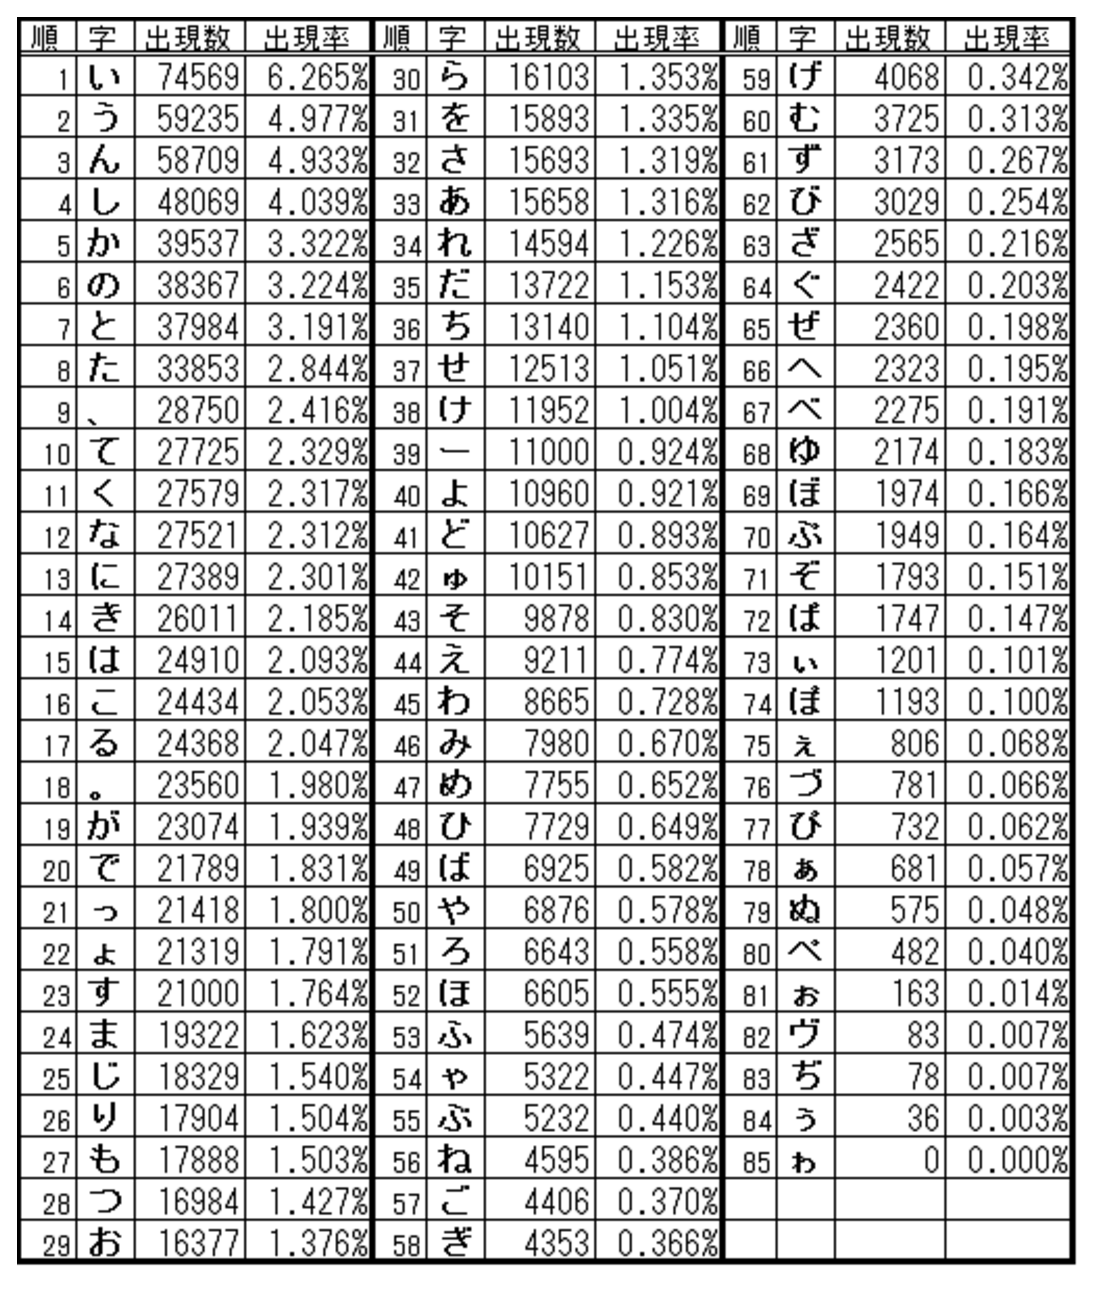
\includegraphics[width=14cm,clip]{res_kouy/1gram.eps}
 \end{center}
 \caption{����100�������̂��ȏo����}
 \label{1gram}
\end{figure*}

���̂悤�ɁA���Ȃ̏o�����͂��Ȃɂ���đ傫���قȂ�܂��B���������āA�o���񐔏�ʂ̂��Ȃ��A�L�[�{�[�h�̑ł��₷���L�[�ɔz�u����΁A�����悭���͂��邱�Ƃ��ł���悤�ɂȂ�܂��B�ł́A�L�[�{�[�h�̑ł��₷���L�[�͂ǂ̃L�[�ł��傤���H

�L�[�{�[�h�̃L�[��łŽw�͕Ў�ɂ‚�5�{����܂��B���̂����e�w�̓L�[�{�[�h�ʼn��i�̃L�[��S�����邷��̂łƂ肠���������܂��B�����L�[��łŽw�͐l�����w�A���w�A��w�A���w��4�{�ł��B���̒��ŃL�[��ł��₷���w�͂ǂ̎w�ł��傤���H�@�l�����w�⒆�w�͓������₷���A�͂�����̂őł��₷���w�ł��B�t�ɁA���w���w�͎v���悤�ɓ��������A���₷���̂őł��ɂ����w�ł��傤�B

�܂��A�L�[�{�[�h�̕����L�[��4�i�ɂ킽���Ĕz�u����Ă��܂��B�u�ŏ�i�v�i�L�[�̍����珇��\key{1}\key{2}\key{3}\key{4}\key{5}�c�c�ƕ���ł���i�j�A�u��i�v�i������\key{Q}\key{W}\key{E}\key{R}\key{T}�c�c�j�A�u�z�[���i�i���i�j�v�i������\key{A}\key{S}\key{D}\key{F}\key{G}�c�c�j�A�u���i�v�i������\key{Z}\key{X}\key{C}\key{V}\key{B}�c�c�j��4�i�ł��B���̂����ł��ł��₷���L�[�̒i�́A��͂�w�𓮂����Ȃ��Ă��ރz�[���i�̃L�[�ł��傤�B����1�i�w�𓮂����K�v�������i�����i�B�ŏ�i��2�i�w�𓮂����K�v������̂ōł��ł��ɂ����i�ł��B

����ɁA�L�[�̉��̃Y����w�̒����Ȃǂɂ���đł��₷�����ς��܂��B�}\ref{key_utiyasusa}�͂킽�����v���e�L�[�̑ł��₷�������������̂ł��B�ł��₷�����Ɂu���A���A���A�~�v�ł��B
���̕\�́��⁛�̂‚����L�[�𑽂��g���A����~�̂‚����L�[�����܂�g��Ȃ��悤�ɂ���΁A�����悭���͂��邱�Ƃ��ł��܂��B


\begin{figure*}
 \begin{center}
   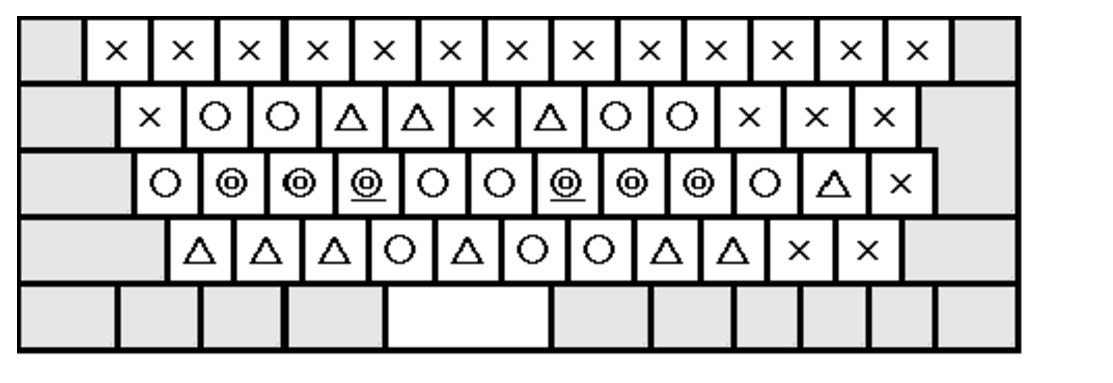
\includegraphics[width=14cm,clip]{res_kouy/key_utiyasusa.eps}
 \end{center}
 \caption{�e�L�[�̑ł��₷��}
 \label{key_utiyasusa}
\end{figure*}

���̂悤�ɁA�V�z��͓��{��ƃL�[�{�[�h�𕪐͂��č��܂��B�V�z��ōl������v�f���g�����̏o�����h�Ɓg�L�[�̑ł��₷���h�Ƃ���2��ނ��Љ�܂������A���ɂ�2�����ȏ�ŘA�����ďo�����邱�Ƃ������A�Ȃ�i�Ⴆ�΁A�u�傤�v�u�Ă��v�u�����v�Ȃǂ͏o�����������j��A�ǂ��o������t���[�Y�i�u�܂��B�v�u�Ƃ����v�Ȃǂ͏o�����������j���l�����܂��B�܂��A1�L�[�ł̑ł��₷���̂ق��ɁA�A�����ăL�[��łꍇ�̑ł��₷�����l�����܂��i�Ⴆ�΁A\key{K}\key{J}�Ƃ����L�[�̘A���͔��ɑł��₷���B\key{M}\key{U}�̂悤�ɓ����w�ʼn����L�[�𑱂��đłƒL�[�̘A���͑ł��ɂ����j�B

�}\ref{dakensuu_ro-maji}�`\ref{dakensuu_keinarabe}�́A�}\ref{1gram}�̃f�[�^���g�p���āA1�����i���ȂŐ����āj�̕��͂���͂����ꍇ�Ɋe�L�[������Ō����邩��z��ʂɎ��������̂ł�\footnote{�}���̃L�[�{�[�h�O�̐����̈Ӗ��F���̏�i�͏��w�E��w�E���w�E�l�����w�̑Ō����A���̉��i�͏�i�̍��v�A�E�͍ŏ�i�E��i�E���i�E���i�̑Ō����A�E���̏�i�͒ʏ�̃V�t�g�⓯���Ō��V�t�g��0�Ō��Ɛ������ꍇ�̑Ō����A�E���̉��i�͒ʏ�̃V�t�g�⓯���Ō��V�t�g��1�Ō��Ɛ������ꍇ�̑Ō����B}�B�}�����Ă��������ƁA�}\ref{dakensuu_ro-maji}�i���[�}�����́j�A�}\ref{dakensuu_JIS-kana}�i���ȓ��́j�ɔ�ׁA�}\ref{dakensuu_NICOLA}�`\ref{dakensuu_keinarabe}�̐V�z��3��i�e�w�V�t�g�A���z��A�����Ȃ�ׁj�̓z�[���|�W�V�����̃L�[�𑽂��g���̂��킩��Ǝv���܂��B

���{��ŗǂ��o�Ă��镶����ł��₷���L�[�œ��͂ł���B������V�z��͑ł��₷���̂ł��B

\begin{figure*}
 \begin{center}
   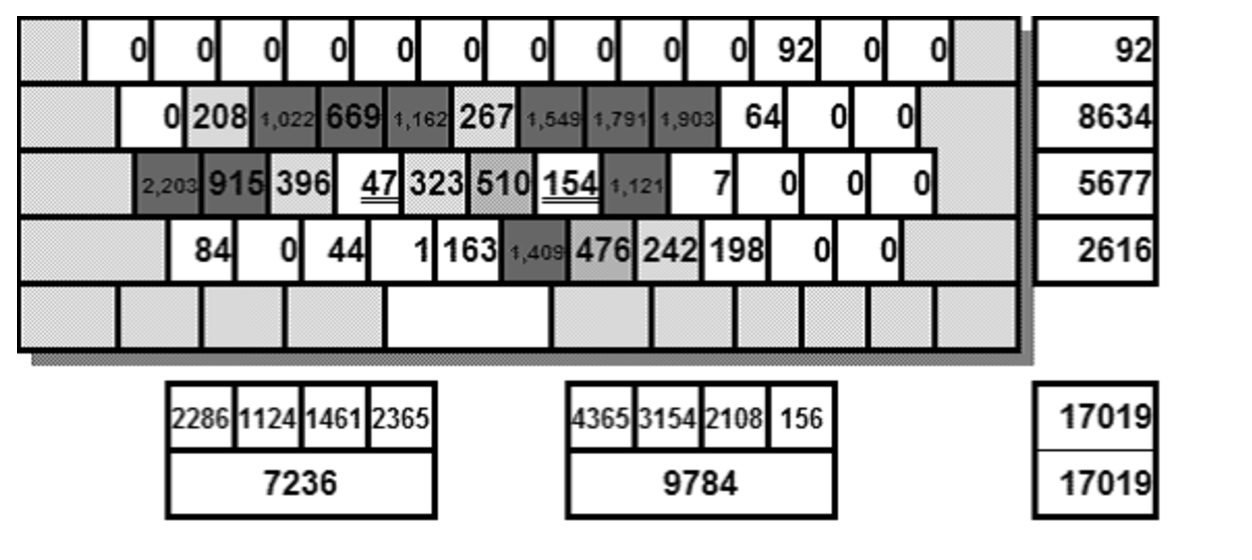
\includegraphics[width=14cm,clip]{res_kouy/dakensuu_ro-maji.eps}
 \end{center}
 \caption{1�����̕��͂���͂����ꍇ�̑Ō����@���[�}������}
 \label{dakensuu_ro-maji}
\end{figure*}

\begin{figure*}
 \begin{center}
   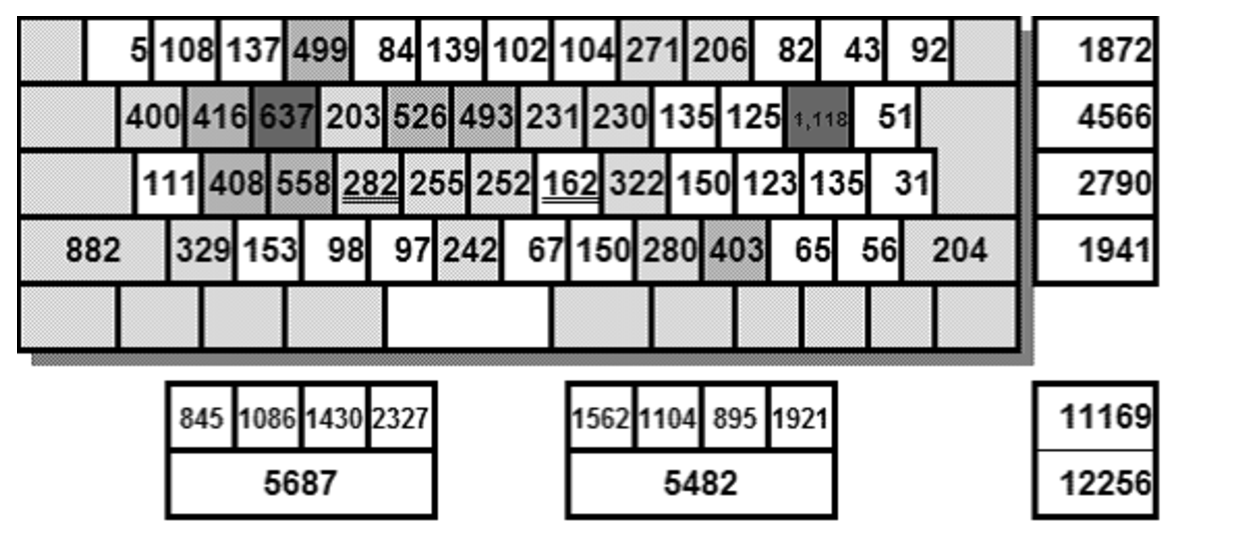
\includegraphics[width=14cm,clip]{res_kouy/dakensuu_JIS-kana.eps}
 \end{center}
 \caption{1�����̕��͂���͂����ꍇ�̑Ō����@���ȓ���}
 \label{dakensuu_JIS-kana}
\end{figure*}

\begin{figure*}
 \begin{center}
   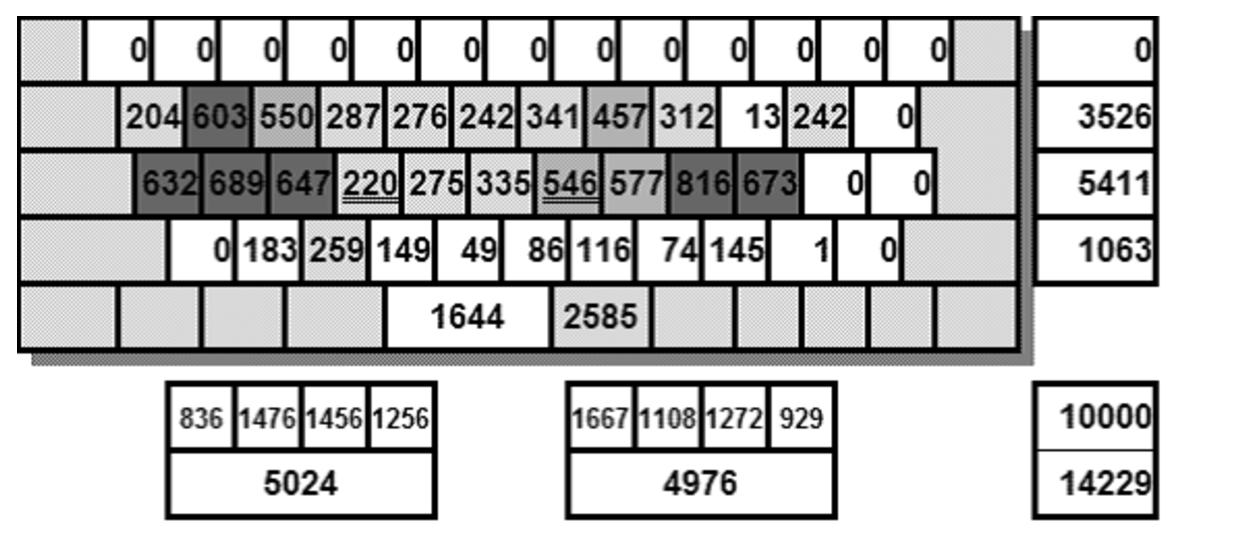
\includegraphics[width=14cm,clip]{res_kouy/dakensuu_NICOLA.eps}
 \end{center}
 \caption{1�����̕��͂���͂����ꍇ�̑Ō����@�e�w�V�t�g�iNICOLA�j}
 \label{dakensuu_NICOLA}
\end{figure*}

\begin{figure*}
 \begin{center}
   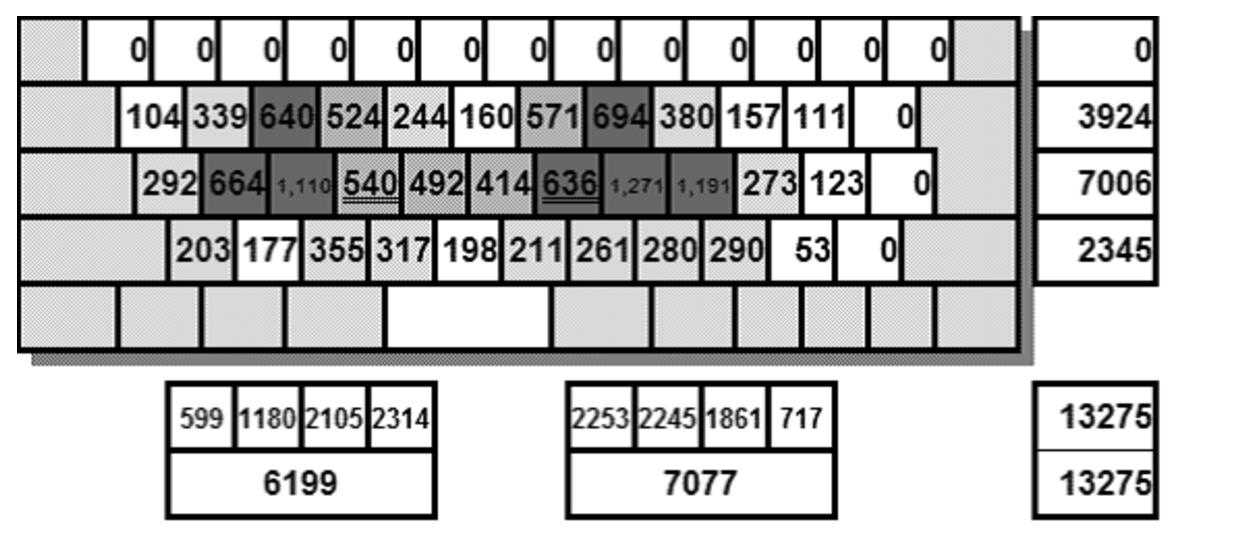
\includegraphics[width=14cm,clip]{res_kouy/dakensuu_tuki2-263.eps}
 \end{center}
 \caption{1�����̕��͂���͂����ꍇ�̑Ō����@���z��2-263��}
 \label{dakensuu_tuki2-263}
\end{figure*}

\begin{figure*}
 \begin{center}
   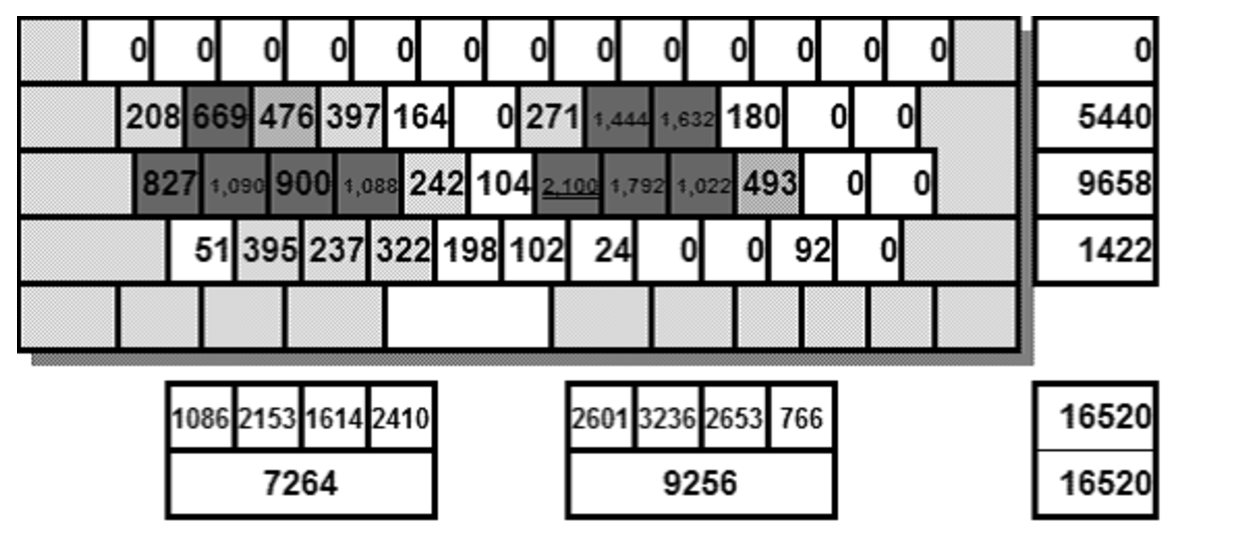
\includegraphics[width=14cm,clip]{res_kouy/dakensuu_keinarabe.eps}
 \end{center}
 \caption{1�����̕��͂���͂����ꍇ�̑Ō����@�����Ȃ��}
 \label{dakensuu_keinarabe}
\end{figure*}

\section{�Ȃ����A�V�z�񂩁H}

�V�z�񂪗D��Ă���ƌ����Ă��A�����p�\�R�����C���^�[�l�b�g������I�ɐG��鐢�̒��B���[�}�����͂Ɋ���Ă��ĉ��̕s�s�����Ȃ��g���Ă���̂ɁA������V�z��Ȃ�āc�c�Ǝv���������邩������܂���B

�������A�p�\�R���ƃC���^�[�l�b�g�����y�����������炱���A�V�z��͒a�����A�g���₷���Ȃ����ƌ�����̂ł��B�u������V�z��v�ł͂Ȃ��u�������V�z��v�Ȃ̂ł��B

\subsection{���܎g���Ă���p�\�R���ŐV�z����g����悤�ɂȂ���}

1980�N�ォ��1990�N��ɂ����āA�p�\�R�������y����O�ɁA���[�v����p�@�����y���Ă������オ����܂����B���[�v����p�@�̎���̔z��̑I���́A���̃��[�v���ɓ��ڂ���Ă���z����g����������܂���ł����B�����̃��[�v���ł̓��[�}�����͂Ƃ��ȓ��͂������ڂ���Ă��܂���ł����̂ŁA�g�p�ł���z��͎����ケ��2��ނɌ��肳��Ă����̂ł��B

���������[�}�����͂Ƃ��ȓ��͈ȊO�ɁA�e�w�V�t�g�iNICOLA�j��VJIS�z��Ƃ������u�V�z��v�͑��݂��Ă��܂����B�������A�e�w�V�t�g���g�����Ǝv������x�m�ʂ�OASYS���A�VJIS�z����g�����Ǝv�����炻�ꂪ���ڂ���Ă���ꕔ�̋@����w�����邵������܂���ł����B�܂��Ă�A�����ŃI���W�i���̔z������Ȃǖ����ꂾ��������ł��B

���݂Ȃ�A�w�������̃p�\�R���Ɏg�������V�z�񂪓��ڂ���Ă��Ȃ��Ă��A���Ƃ���lj����Ď������邱�Ƃ��ł��܂��B

�z�����������\�t�g�E�F�A���g�p����ƁA���g���Ă���p�\�R���A���g���Ă���L�[�{�[�h�̂܂܂ŐV�z����g�p���邱�Ƃ��ł��܂��B���̂悤�ȐV�z�����������\�t�g�E�F�A�̂��Ƃ��u�z��G�~�����[�^�v�ƌĂт܂��i�ȉ��A�P�ɃG�~�����[�^�Ƃ������܂��j�B�G�~�����[�^�͂��܂��܂Ȏ�ނ̕�������A�����Ŏg�����Ƃ��ł�����̂�����܂��B�܂��A�C���^�[�l�b�g��ʂ��ă_�E�����[�h�ł���̂ŁA����ł��ȒP�ɓ���ł��܂��B����ɁA�ꕔ�̐V�z��́A�G�~�����[�^���g���܂ł��Ȃ��AIME���g���Ď����ł�����AOS�ɍŏ����瓋�ڂ���Ă�����̂�����܂��B

�V�z��𓱓����邽�߂̃n�[�h���́A�̂ɔ�ׂ͂邩�ɒႭ�Ȃ����̂ł��B

\subsection{���l�Ȕz�񂪐��܂�Ă���}

�p�\�R���ƃC���^�[�l�b�g�ɂ��V�z�񂪎󂯂����b�́A���ꂾ���ł͂���܂���B

�O�q�̒ʂ�A���݂ł̓G�~�����[�^���g���ΊȒP�ɐV�z����������邱�Ƃ��ł��܂��B�����ăG�~�����[�^�̑����́A�����̔z�u�����R�ɓ���ւ�����Ƃ����@�\������Ă��܂��B���̋@�\�ɂ��A���‚Ă͖����ꂾ�����u�����ŃI���W�i���̔z������v���Ƃ��ł���悤�ɂȂ�܂����B�u��������΂����Ɨǂ��Ȃ�v�Ǝv���_���C��������A�ꂩ��܂������V�����z������Ƃ������Ƃ��A�ȒP�ɂł���悤�ɂȂ����̂ł��B

����ɂ��A2000�N�O�ォ�猻�݂ɂ����āA�������̐V�z�񂪐��ݏo�����悤�ɂȂ�܂����B�����͌l�ɂ���č��ꂽ���̂ł����A�C���^�[�l�b�g����炵���A�l�b�g��Ɍ��J����A�����̐l�̈ӌ���������ď������C�����č��ꂽ�V�z�������܂��B

�V�z������ɂ́A��ɂ��������ʂ���{��̕��͂��s�Œ��ł��B���‚ẮA���{��̕��͂��̏W���āA�������͂���Ƃ����̂͑�ςȎ�Ԃ��������Ƃł����B

�������A���ꂳ�����p�\�R���ƃC���^�[�l�b�g���������Ă��܂��܂����B���݂ł́A�z�����邽�߂ɕK�v�ȓ��{��̃f�[�^�̓C���^�[�l�b�g��Ō��J����Ă��܂��B���‚Ă͌l�ł͂ƂĂ���ɕ����Ȃ������悤�ȃf�[�^���A�ȒP�Ɏ�ɓ���邱�Ƃ��ł���̂ł��B����ɕK�v�Ȃ�A�����œ��{��𕪐͂��邱�Ƃ��ł��܂��B���̂��߂ɕK�v�ȕ��͉�̓c�[�����A�l�b�g����_�E�����[�h�ł���̂ł��B

���炽�ȐV�z�񂪎��X�ƒa���������Ƃɂ��A�V�z��̑I�����͑傫���L����܂����B���‚Ă̓��[�}�����͂₩�ȓ��͈ȊO�̔z��ƌ����΁A�e�w�V�t�g���炢�����I����������܂���ł����B���݂ł́A�e�w���V�t�g�Ƃ���z��A���w���V�t�g�Ƃ���z��A�����Ō����g���z��E�g��Ȃ��z��A�o���₷���ɏd�_��u�����z��ȂǁA���ꂼ��ɗD�ꂽ�����̂���z�񂪑������ݏo����Ă��܂��B21���I�ɓ����Ă���10�N�ȏオ�o���A�V�z��͂܂���\ruby{�S��㇗�}{�Ђ������傤���}�B���낻���v�ȃA�C�f�A���o�s�����A�~�n�����}�����ƌ�����Ǝv���܂��B

���Ȃ�A���Ȃ����C�ɂ���V�z�񂪂����ƌ��‚���͂��ł��B

\section{���Ȃ�V�z�񂾂��Ċo������}

�V�z�񂪑䓪���Ă����̂͂킩��������ǁA���łɃ��[�}�����͂Ɋ���Ă��邵�A���܂�����͕��@��ς���C�ɂ͂Ȃ�Ȃ��A�Ǝv������������������܂���B

���߂ăp�\�R����G�����Ƃ��A�L�[�{�[�h�̓��͂ɋ�킵���L���͒N�ɂł�����Ǝv���܂��B�ǂ��ɉ��̃L�[������̂��܂�����������Ȃ��B1�������͂��邲�ƂɃL�[�{�[�h����ړI�̃L�[����ˆ�’T���o���B�u����ɂ��́v��1����͂��邾���ł����J�B�V�z����g���Ƃ���ƁA�܂����̌o�����J��Ԃ��Ȃ���΂Ȃ�Ȃ��̂��B��������ȋ�J�͂܂��҂��ƁA�Ǝv���C�������킩��Ȃ��ł͂���܂���B

�������A�m���ɐV�z����g�����Ȃ��ɂ͈��̗��K���K�v�ł����A�V�z��̏K���͂���قǑ�ςȂ��Ƃł͂���܂���B���߂ăp�\�R���ɐG�ꂽ�Ƃ��Ƀ��[�}�����͂��o�����Ƃ��Ɣ�ׂ�΁A�����ƊȒP�Ɋo���邱�Ƃ��ł��܂��B

\subsection{�L�[�{�[�h�Ɋ���Ă���}

�V�z��̏K�����ȒP�ȑ��̗��R�́A���łɃL�[�{�[�h���̂ɂ͊���Ă���Ƃ������Ƃł��B�݂Ȃ���̓��[�}�����͂Ȃ肩�ȓ��͂Ȃ�ŁA�L�[�{�[�h�ŕ�������͂���Ƃ������Ǝ��̂́\�\���ꂼ��ɒ��x�̍��͂���ł��傤���\�\�K������Ă���Ǝv���܂��B

�p�\�R���ɐG�ꂽ�����A�L�[�{�[�h�ɏ��߂ĐG�ꂽ�Ƃ��ɕ������͂ɋ�J�����̂͂Ȃ��ł��傤���H�@�������A�ǂ̃L�[���ǂ��ɔz�u����Ă��邩������Ȃ��Ƃ������R������ł��傤�B�������A�L�[�{�[�h���̂Ɋ���Ă��Ȃ����Ƃ��傫�ȗ��R�������͂��ł��B�������Ƃ��Ă���L�[��ڂŌ��āA�ʒu���m�F���Ȃ��Ƃ��̃L�[�������Ȃ��B�L�[�{�[�h�����Ȃ��őłƂ��Ƃ��Ă��A�ǂ̎w���ǂ̂��炢�������΂ǂ̃L�[��������̂��A�ǂ̂��炢�̋����ʼn����΂����̂��A�܂������������‚��Ȃ��B�������‚���ʼn����Ă��Ȃ�������A�����Ă��Ȃ��͂��̂̃L�[��������Ă����肷��B�������肷��ƃL�[�̊ԂɎw��������2�ƒL�[�������Ă��܂��c�c�B�ŏ��͂���ȏ�Ԃ������Ǝv���܂��B

�L�[�{�[�h�Ɋ��ꂽ���Ȃ�A����Ȃ��Ƃ͂���܂���B�L�[�{�[�h�ɑ΂��銴�o�͂��łɐg�ɂ‚��Ă��܂��B�ǂ̃L�[��łĂ΂����̂�������΁A�ړI�̃L�[��ł‚��Ƃ͊ȒP�ɂł��܂��B���̊��o�͐V�z��ł����̂܂܎g�����Ƃ��ł��܂��B

����ɁA���łɃp�\�R���̑���Ɋ���Ă���Ƃ������R������܂��B�p�\�R���ɐG�ꂽ�����́A�ǂ̃L�[���������牽���N����̂��\���ł��Ȃ���Ԃł��B1�ƒL�[�������ԈႦ�������Œv���I�Ȏ��Ԃ��N���邩������Ȃ��B�Ԉ�����L�[���������Ƃ��A�ǂ�����ΏC���ł���̂����킩��Ȃ��B������ԈႦ�����Ȃ��B����ƁA���������m�F���Ȃ��ƃL�[�������Ȃ����A��������ԈႦ��ƏC���Ɏ��Ԃ�������܂��B����ł͂Ȃ��Ȃ����͂��i�܂��A�Ȃ��Ȃ�����邱�Ƃ��ł��܂���B

���Ȃ炻��Ȃ��Ƃ͂���܂���B�Ƃ肠�����J�`���J�`���Ɠ��͂��āA�Ԉ���Ă����璼���Ηǂ������̂��Ƃł��B�ǂ�ǂ�L�[��ł��Ăǂ�ǂ�C�����Ă����΁A�����Ɋ���邱�Ƃ��ł��܂��B

���߂ɔz����o�����Ƃ��Ƃ����̂́A���͔z��ȊO�̂��Ƃ������Ɋo���Ă����̂ł��B���Ȃ�A�L�[�{�[�h�ɂ͊���Ă��邵�A�p�\�R���̑����������܂��B�z����o���邱�Ƃ����ɏW���ł���̂ł��B

\subsection{�ł��₷���L�[�𑽂��g��}

�V�z��̏K�����ȒP�Ȃ�����‚̗��R�́A�V�z��͑ł��₷���L�[�𑽂��g���Ƃ������Ƃł��B�L�[�{�[�h�̃L�[�̒��ɂ́A�ł‚̂��ȒP�ȃL�[�Ɠ���L�[������܂��B�ł‚̂��ȒP�ȃL�[�𑽂��g���قǏK�����₷���Ȃ�܂��B

�ł́A�ł‚̂��ȒP�ȃL�[�Ƃ͂ǂ̃L�[�ł��傤���H�@�z�[���|�W�V�����ł͂Ȃ��L�[��łꍇ�́A�w�����̃L�[�̏�ɐ��m�ɓ������Ȃ���΂����܂��񂩂�A�ł‚̂�����Ȃ�܂��B�܂��A���w�͗͂��キ�ق��̎w�ɔ�ׂĎg���ɂ����̂ŁA���m�ɃL�[��ł‚̂�����w�ł��B�t�ɁA�w���L�[�̏ォ�瓮�������ɍςރz�[���|�W�V�����̃L�[���A�������₷���l�����w�E���w�E��w���g���đłꍇ�́A�ȒP�ɑł‚��Ƃ��ł��܂��B
����āA�ł��ł‚̂��ȒP�ȃL�[�́A�l�����w�E���w�E��w�̃z�[���|�W�V�����̃L�[�A��̓I�ɂ�\key{S}\key{D}\key{F}�A\key{J}\key{K}\key{L}��6�L�[�ƂȂ�܂��B

�������A���[�}�����͂ł͂����̃L�[�̎g�p���͂��܂荂������܂���B���[�}�����͂ōł��悭�g���L�[�́A�ꉹ�L�[�A���Ȃ킿\key{A}\key{I}\key{U}\key{E}\key{O}��5�L�[�ł��B����5�L�[�́A��قNj������ł‚̂��ȒP��6�L�[�ɂ͈�‚��܂܂�Ă��܂���B�‚܂胍�[�}�����͂́A�ł‚̂��ȒP�ȃL�[�����܂�g�킸�A������ł‚̂�����L�[��p�ɂɎg���z��Ȃ̂ł��B����ł͏K��������Ȃ�̂��K�R�ł��B

���ȓ��͂��A�ł‚̂��ȒP�ȃL�[�𑽂��g���Ƃ͌����Ȃ��z��ł��B�z�[���i����i�̕����g�p��������������A�ŏ�i�ɂ��g�p�������Ȃ荂���L�[����������A���|�I�ɏo�������������_���z�[���|�W�V��������O�ꂽ�A���������w���S������L�[�ɔz�u����Ă����肵�܂��B�w���z�[���|�W�V�������痣��ĉ����̃L�[��ł��ɍs���@������̂ł�����A���G�Ȏw�̓����������A��x���A�b�v���܂��B

�w�𓮂����Ȃ��čςރz�[���|�W�V�����̃L�[�𑽂��g���A�����w�ňقȂ�L�[�𑱂��đł‚悤�ȕ��G�ȓ���͂ł��邾�����Ȃ��B����Ȕz��Ȃ�A�K������̂͂����ƊȒP�Ȃ��ƂɂȂ�܂��B

�V�z��́A���{��ő����o�����镶������͂��₷���悤�ɔz�u���Ă��܂��B�K�R�I�ɁA�ł��₷���L�[�̎g�p���������Ȃ�A���G�Ȏw�̓��������Ȃ��Ȃ�܂��B����͓��͂��������I�ɂł���悤�ɍH�v�������ʂł����A���̂悤�Ȕz��́\�\�K��������Ɍ����I�ɓ��͂ł��邾���łȂ��\�\�K�����邱�Ǝ��̂��Ղ����Ȃ�̂ł��B

\section{�V�z��FAQ}

\subsection{�V�z������܎g���Ă���p�\�R���Ŏg����H}

\subsubsection*{�y����z}

�V�z����g���ɂ́A�V���Ƀp�\�R����L�[�{�[�h�Ȃǂ𔃂��K�v������̂ł����H�@�V�z������܎g���Ă���p�\�R���Ŏg���ɂ͂ǂ�������悢�ł����H

\subsubsection*{�y�񓚁z}

�z���OS�ɂ���Ă��܂��܂Ȏ������@������܂����A�z��G�~�����[�^�ƌĂ΂��\�t�g�E�F�A���g���ĐV�z�����������̂��ȒP�ȕ��@�ł��B�G�~�����[�^���g���΁A���܎g���Ă���p�\�R���A�L�[�{�[�h���g�p�����܂ܐV�z����g�p���邱�Ƃ��ł��܂��B�V���Ƀp�\�R����L�[�{�[�h���w������K�v�͂���܂���B

�G�~�����[�^�͂��܂��܂Ȏ�ނ̂��̂����݂��܂��B�ȉ��ɑ�\�I�Ȕz��G�~�����[�^�������܂��B

\begin{itemize}
 \item �w�P�x�q���x�i�V�F�A�E�F�A�j
 \item �wDvorakJ�x�i�t���[�\�t�g�j
 \item �w��܂Ԃ��x�i�t���[�\�t�g�j
\end{itemize}

�܂��A�z��G�~�����[�^�̂ق��ɁA�L�[�J�X�^�}�C�Y�\�t�g�i�L�[�o�C���h�ύX�\�t�g�j�ƌĂ΂��W�������̃\�t�g������܂��B�z��G�~�����[�^����ɃL�[���������Ƃ��ɓ��͂���镶����ύX����̂ɑ΂��A�L�[�J�X�^�}�C�Y�\�t�g�̓L�[�̋@�\���̂��̂�ύX���܂��B�������A�z��G�~�����[�^�ŃL�[�̋@�\��ύX�ł�����A�L�[�J�X�^�}�C�Y�\�t�g�ł����͂���镶����ύX�ł�����̂�����̂ŁA���̋��ڂ͂����܂��ł��B�ȉ��A��\�I�ȃL�[�J�X�^�}�C�Y�\�t�g�������܂��B

\begin{itemize}
 \item �w�̂ǂ��x�i�V�F�A�E�F�A�j
 \item �wYet Another Mado tsukai no Yuutsu�x�i�t���[�\�t�g�j
 \item �w���g���̗J�T�x�i�t���[�\�t�g�j
 \item �wKeySwap for XP�x�i�t���[�\�t�g�j
 \item �wKeyRemap4MacBook�x�i�t���[�\�t�g�j
\end{itemize}


\subsection{�ق��̃p�\�R�����g�����ɍ���Ȃ��ł����H}

\subsubsection*{�y����z}

�V�z����g���ɂ̓G�~�����[�^�Ȃǂ��g�p����K�v�����邻���ł����A��������Ǝ����̃p�\�R�����g���Ƃ��͂悢�ł����A�ق��̃p�\�R�����g���Ƃ��ɐV�z����g�����Ƃ��ł��Ȃ��̂ł͂Ȃ��ł����H�@����͍���܂��񂩁H

\subsubsection*{�y�񓚁z}

�V�z�����������ɂ̓G�~�����[�^�Ȃǂ��g�p����K�v������܂����A�G�~�����[�^��USB�������Ȃǂɓ���Ď����^�ׂ�^�C�v�̂��̂�����܂��B����𗘗p����΁A�ǂ̃p�\�R���ł��V�z��𗘗p���邱�Ƃ͉”\�ł��B

�܂��A�V�z����g���Ȃ��󋵂ł́A���̂Ƃ��������[�}�����͂��g�p���邱�Ƃɂ���Ζ�肠��܂���B����FAQ�������������B

\subsection{���[�}�����͂ƐV�z��𕹗p�ł��܂����H}

\subsubsection*{�y����z}

�V�z����o���Ă��A���[�}�����͂��g�����Ƃ͂ł��܂����H�@���[�}�����͂�Y��Ă��܂����Ƃ͂���܂��񂩁H

\subsubsection*{�y�񓚁z}

�V�z����o���Ă��A���܂܂Ŏg���Ă������[�}�����͂͂��̂܂܎g�����Ƃ��ł��܂��B��x���]�Ԃ̏������o����ƁA���΂炭���]�Ԃɏ��Ȃ����Ԃ������Ă������͖Y��Ȃ��A�Ƃ������ۂɎ��Ă��܂��B

���ہA�V�z����g���Ă���l�̑����́A�K�v������΃��[�}�����͂œ��͂��Ă��܂��B�킽���������̃p�\�R���ȊO�œ��͂���K�v������Ƃ��̓��[�}�����͂��g�p���Ă��܂����A�܂��������Ȃ��g�p�ł��܂��B

\subsection{���[�}�����͂̓A���t�@�x�b�g�̔z�u���g���邩��ǂ��̂ł́H}

\subsubsection*{�y����z}

�p�\�R���̕������͂ł́A���Ȃ̓��͂̂ق��ɃA���t�@�x�b�g�̓��͂��g���܂��B���[�}�����͂Ȃ�A���t�@�x�b�g�̔z��1�‚ł��Ȃ��A���t�@�x�b�g�����͂ł���̂ŁA��͂胍�[�}�����͂��g���̂������I�ł͂Ȃ��ł��傤���H

\subsubsection*{�y�񓚁z}

���[�}�����͂̏K����ʂ��ăA���t�@�x�b�g�̔z�u��������x�o���邱�Ƃ��ł��܂��̂ŁA�p�\�R�����S�҂̒i�K�A�‚܂肩�Ȃ̓��͂��A���t�@�x�b�g�̓��͂��o�����ĂȂ��Ƃ����i�K�ł́A�m���Ƀ����b�g�͂���Ǝv���܂��B���߂ăp�\�R���ɐG�����l�����[�}�����͂��o����Ƃ����̂́A���̍�����������Ǝv���܂��B

�������A����ȏ�̒i�K�ɂȂ�ƁA���[�}�����͂�ʂ��ăA���t�@�x�b�g�̓��͂���K�ł���Ƃ������ʂ͂قƂ�ǖ����Ȃ��Ă��܂��B���[�}�����͂Ɋ���Ă���ƁA���[�}�����͂�����ۂł��A���t�@�x�b�g���قƂ�Ljӎ����Ȃ��œ��͂ł���悤�ɂȂ�܂��B�u���v�Ɠ��͂���Ƃ��ɁA\key{K}��\key{A}��ł‚ƈӎ�����̂ł͂Ȃ��A�P�Ɂu���v�̓��͂ɕK�v��2�‚̃L�[��ł‚Ƃ������o�ɂȂ�܂��B�A���t�@�x�b�g���ӎ����Ȃ��̂ł�����A���[�}�����͂��g�������Ă��A�A���t�@�x�b�g�̓��͂���B���邱�Ƃ͂���܂���B�p����͉͂p����͂ŁA���[�}�����͂Ƃ͕ʂɏK������K�v������܂��B

����āA�A���t�@�x�b�g�̓��͂��g���Ƃ��Ă��A���[�}�����͂��L���Ƃ������Ƃ͂���܂���B���Ȃ̓��͕��@�̓A���t�@�x�b�g�̓��͂Ƃ͐؂藣���āA�����܂Łg���Ȃ̓��́h�����₷�����@��I�ԕ��������I���Ǝv���܂��B

\subsection{�V�z����o����̂ɂǂꂭ�炢�̎��Ԃ�������܂����H}

\subsubsection*{�y����z}

�V�z����g���Ă�����x���炷����͂ł���悤�ɂȂ�܂ŁA�ǂꂭ�炢�̎��Ԃ�������܂����H

\subsubsection*{�y�񓚁z}

���K���@��A�ǂꂭ�炢�W�����ė��K�ł��邩�A�o����V�z��̓�x�Ȃǂɂ���ĈقȂ�܂����A����܂ł̐V�z����o�����l�̑̌��k�ɂ���2�T�ԁ`2�����قǂ̂悤�ł��B

�V�z����K������܂ł́A�傫��2�‚̃X�e�b�v�ɕ�����܂��B1�–ڂ��u���̃X�e�b�v�v�\�\�z��}�𓪂̒��ɓ����\�\�A2�–ڂ��u�w�̃X�e�b�v�v�\�\���镶������͂��悤�Ǝv�����Ƃ��Ɏw���u���ɂ��̃L�[�łĂ�悤�ɂȂ�\�\�A�ł��B�u���̃X�e�b�v�v�ɂ�������Ԃ͔z��ɂ���đ傫���قȂ�܂��B�܏\�����ɕ��ׂ��悤�ȒP���Ȕz��Ȃ炷���ɂł��o������ł��傤�B�o����v�f�������Ȃ�قNJo����̂�����Ȃ�܂��B�l�l�̋L���͂���K�̏W���x�ɂ���Ă��قȂ�ł��傤�B�u�w�̃X�e�b�v�v�Ɋւ��ẮA�z��̍��͂���قǂ���܂���B�P���Ȕz��ł����Ă��w�����������Ȃ�悤�ɂȂ�܂łɂ͂�����x�̗��K���K�v�ł��B����΂���͂Ƃɂ����g���Ċ���邵���Ȃ��悤�ł��B

�ŏ��͎w�������Ȃ��ċ�J����Ǝv���܂����A�������͑��x���オ��Γ������K���Ԃō��܂ł�葽���̗��K���ł��邱�ƂɂȂ܂��B����Ɨ��K�������ǂ��Ȃ�A���̌��ʓ��͑��x���オ���āA����ɗ��K�������ǂ��Ȃ�c�c�Ɖ����x�I�ɓ��͑��x���オ���Ă����܂��B�����Ȃ�ΐV�z��K���ԋ߂ƌ�����ł��傤�B

�V�z����o����R�c����B�V�z��ł͗ǂ��o�����邩�Ȃ͑ł��₷���L�[�ɔz�u����Ă��܂��B���������āA�ǂ��o�����邩�Ȃ�T���Ƃ��͑ł��₷���L�[�A���܂�o�����Ȃ����Ȃ�T���Ƃ��͑ł��ɂ����L�[��T���ƌ��‚���₷���Ȃ�܂��B

�ǂ̂��Ȃ��ǂ��o������̂��\�\��Ɍf�ڂ����}1-1�̒ʂ�ł����\�\������Ȃ��Ǝv����������܂���B���������ςɌ����ƁA�܏\���\�̍ŏ��̕��ɏo�Ă��邩�Ȃ͗ǂ��o�Ă��܂��i�������A�u��v�͍ŕp�o���Ȃ̈�‚ł��j�B���������ڂ��������ƁA���s�`���s�͂قڂ��ׂďo������ʂ̂��Ȃł��B�ȍs�́u�ȁv�u�Ɂv�Ɓu�́v�A�͍s�́u�́v�����B���̂��炢�܂ł��o�����������ƌ����邩�Ȃł��B��O�͂���܂����A���ꂾ���ł��V�z����o���鏕���ɂ͂Ȃ�Ǝv���܂��B

\subsection{�V�z��̗��K���@�͂ǂ�����΂悢�ł����H}

\subsubsection*{�y����z}

�V�z��̗��K�͂ǂ̂悤�ȕ��@�ōs���΂悢�ł��傤���H

\subsubsection*{�y�񓚁z}

�l�l�ōD�݂�‹��A���K�ɂ������鎞�ԂȂǂ��قȂ�܂��̂ŁA�x�X�g�̕��@�͂��ꂼ��قȂ�Ǝv���܂��B�����ł͂킽�����������߂�����@����Љ�܂��B

�܂��A�z��}���ËL���܂��B���̒i�K�ł͎��ۂɃp�\�R�����g�����������͂͂��܂���B�z��}�����ɏ����Ď��������āA�󂫎��ԂɂƂ��ǂ�����悤�ɂ���Ɗo���₷���Ǝv���܂��B�z��}�����������Ɏ��ɏ����邭�炢�܂Ŋo����ƃx�X�g�ł��B�������A�z��}�������珇�Ԃɓǂ�Ŋo����悤�Ȃ����Ŋo���Ă����܂�Ӗ�������܂���B���ȂƃL�[��1��1�Ŋo����悤�ɐS�����Ă��������B

�z��}���o������A�^�C�s���O�Q�[���ŗ��K���܂��B�w�^�C�v�E�F���x�͋L�^���ڍׂɎc���Ď����̐������m�F�ł���̂ł������߂ł��B�܂����ۂ̕��͓��͂ł͎g�p���܂���B���͂��l����Ƃ����̂͑�ςȍ�Ƃł��B�܂�1����1�������͂���̂���ςȒi�K�ł�����A���͂��l���Ȃ���V�z��̗��K������Ƃ����̂́A��ςȍ�Ƃ𓯎��ɍs�����ƂɂȂ�A�ւ������đ�ςȍ�ƂɂȂ�܂��B�^�C�s���O�Q�[���Ȃ���͂��镶���̓Q�[���̕��Ŏ����I�ɒ񎦂��Ă���܂��̂ŁA�����͔z��̗��K�ɏW�����邱�Ƃ��ł��܂��B

���̍ہA�z��}�����S�Ɋo������܂ł́A�z��������������f�B�X�v���C�̋߂��ɓ\���Ă����Ɨǂ��ł��傤�B�������A���͂ł���Ǝv�����玆�����Ȃ��ŃL�[�������Ă��������B�o���Ă���̂Ɏ������Ă��܂��ƁA���͑��x�Ɏ����Ńu���[�L���|���Ă��܂����ƂɂȂ�A�����ɐ��������܂��B�Ƃ肠�����L�[��ł��āA�Ԉ���Ă�����C������΂悢�̂ł��B

�����Ă�����x�̑��x�œ��͂ł���悤�ɂȂ�����\�\�^�C�v�E�F���Ō����Α������x��E���炢�\�\���ۂ̕��͓��͂ł��g�p���n�߂܂��B

���܏Љ�����K���@�͂����܂ň��ł��B�u�v�����������̓����瑦���퓊���I�v�Ƃ������K���@������܂��B���ꂼ��ŗǂ��Ǝv�����@��I��ł��������B

�܂��A���K�p�\�t�g����K�p�e�L�X�g���p�ӂ���Ă���V�z�������܂��B�Ⴆ�΁A�e�w�V�t�g�iNICOLA�j�ɂ́A�w�e�w�V�t�g���K�x�Ƃ������K�p�̃t���[�\�t�g������܂��B�����𗘗p����̂��ǂ��ł��傤�B

\subsection{�K������܂ł̊ԁA����̕��͓��͍�Ƃ��ǂ�����΂悢�ł��傤���H}

\subsubsection*{�y����z}

�V�z����K������܂ł̊ԁA���͓��͑��x���������ቺ����̂���ɂł��B�ǂ����Ă��߂������ɏ����グ�Ȃ���΂����Ȃ����͂�����܂��B�ǂ�����΂悢�ł����H

\subsubsection*{�y�񓚁z}

������x�W�����ė��K�ł�����Ԃ�����΃x�X�g�ł����A���ۂɂ͓���ꍇ�������Ǝv���܂��B�킽���̈ӌ��ł́A�܂��V�z��ł̓��͑��x�ł͎��ۂ̕��͓��͂Ŏg���ɂ͕s�����Ƃ����ꍇ�́A�������Ă܂ŗ��K���̐V�z����g�p���Ȃ��ŁA���[�}�����͂œ��͂��Ă��ǂ��Ǝv���܂��B���[�}�����͂��g�p��������Ƃ����ĐV�z��̗��K���ʂ�������������Ƃ������Ƃ͂���܂���B

�������A���ۂ̕��͓��͂�����K�v���Ȃ��A�V�z��̗��K�ɏW���ł�����Ԃ��m�ۂł���Ȃ炻�ꂪ���z�ł��B�����x�݂Ȃǂ𗘗p����̂���‚̕��@�ł��傤�B

\section{�������ߐV�z��}

����ł͐V�z�񂪂ǂ̂悤�Ȃ��̂Ȃ̂���̓I�Ɍ��Ă����܂��傤�B�V�z��͎����‹��A�K����x�A�z�񗝘_�Ȃǂɂ��A�������̎�ނ�����܂��B�����ł͂킽�����������߂���V�z���5�Љ�܂��B

\subsection{�e�w�V�t�g�iNICOLA�j}

�e�w�V�t�g�͐V�z��̒��ōł��L���Ȕz��ł��B���[�v����p�@�̎��ォ�瑶�݂���z��ŁA���݂ł������̈��p�҂����܂��B

\begin{figure*}
 \begin{center}
   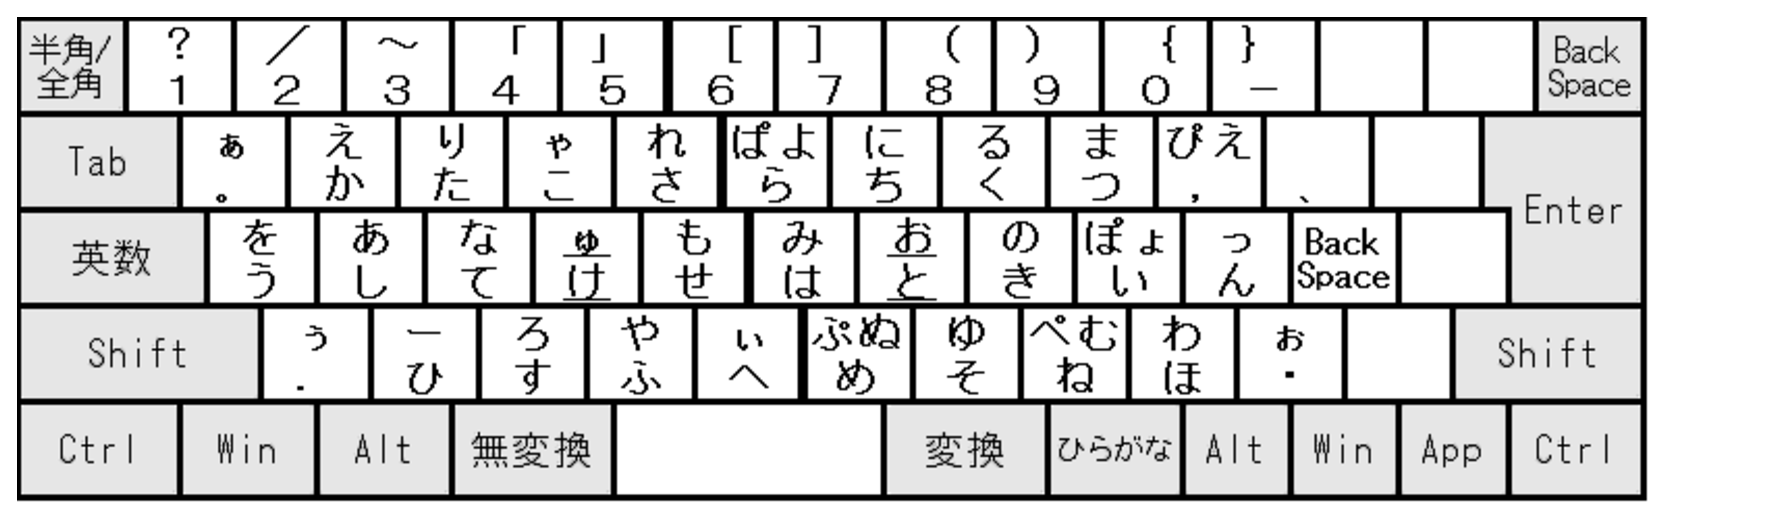
\includegraphics[width=14cm,clip]{res_kouy/NICOLA.eps}
 \end{center}
 \caption{�e�w�V�t�g�iNICOLA�j�z��}}
 \label{NICOLA}
\end{figure*}

\subsubsection*{�e�w���V�t�g�L�[�ɂ���}

�e�w�V�t�g�̍ő�̓����́A�u�e�w�L�[�v���g�p���ĕ�������͂��邱�Ƃł��B

�}\ref{NICOLA}�͐e�w�V�t�g�̔z��}�ł��B1�‚̃L�[��2�‚̕�����������Ă��܂��B�L�[�̉����ɏ����ꂽ�����́A�P�ɂ��̃L�[���������Ƃɂ���ē��͂��܂��i�P�Łj�B�����ăL�[�̏㑤�̕����́A���̃L�[��������Ɠ�����́u�e�w�L�[�v�i�ʏ��\key{���ϊ�}��\key{�X�y�[�X}��\key{�ϊ�}�̂����ꂩ�B���Ƃŏڂ����������܂��j�𓯎��ɉ������Ƃɂ���ē��͂��܂��B�Ⴆ�΁A��i�̍�����2�Ԗڂ̃L�[�i\key{W}�j�ɂ́u���v�Ɓu���v�Ƃ���2��ނ̂��Ȃ�������Ă��܂��B�u���v�Ɠ��͂���Ƃ��́A\key{W}��P�ɉ����܂��B�u���v�Ɠ��͂���Ƃ���\key{W}��\key{���e�w}�𓯎��ɉ����܂��B�܂��A���̃L�[��������Ɣ��΂̎�̐e�w�L�[�𓯎��ɉ������ꍇ�́A�P�łœ��͂ł��邩�Ȃɑ��_���t������������͂��܂��B�Ⴆ��\key{W}��\key{�E�e�w}�𓯎��ɉ����ƁA�u���v�����͂���܂��B���̂悤�ɁA�e�w�V�t�g�ł̓V�t�g���̕�������͂���Ƃ��ɁA�e�w�L�[���g�p���܂��B

���{����͂̍ہA�e�w�S���̃L�[�͂��܂�g���邱�Ƃ̂Ȃ��L�[�ł��B�����ϊ��̂Ƃ��͂�����x�g�p���܂����A���̑��̑���͎g�p���͂���قǍ�������܂���B�p��̏ꍇ�ł��ƃX�y�[�X�͔��ɗǂ����͂���̂Őe�w���g���̂ł����A���{��̕��͂ł̓X�y�[�X�͂��܂�g���܂���B����ł͎w�̔\�͂��\���Ɋ��p�ł��Ă���Ƃ͌����܂���B�e�w�𕶎����͂Ɏg�p���邱�ƂŁA�w�̔\�͂��t���Ɋ��p���邱�Ƃ��ł���悤�ɂȂ�܂��B

\subsubsection*{�����Ō��Ƃ͂ǂ������Ӗ����H}

��قǁu\key{W}��\key{���e�w}�L�[���g�����Ɂh�����܂��v�Ə����܂����B�e�w�V�t�g�ł͐e�w�L�[�ƕ����L�[���u�����Ɂv�Ō�����Ƃ����̂��傫�ȓ����ł��B�u�����ɑŌ�����v�Ƃ����Ɖ������������@�̂悤�ɕ������܂��B�����ł������^�C�~���O�����ꂽ����͂ł��Ȃ��̂��A����ȕ��ɑz�������������邩������܂���B

�������A�����Ō��Ƃ������t�̈Ӗ��́u�ǂ���̃L�[���ɉ����Ă��\��Ȃ��v�Ƃ������Ƃł��B���ʂ̃V�t�g�i�ʏ포�w�ʼn���\key{Shift}�ōs���V�t�g�j�̏ꍇ�́A�L�[���������Ԃ͌��܂��Ă��܂��B�Ⴆ�΃A���t�@�x�b�g�Łi�啶���́j�uA�v�Ɠ��͂���ꍇ�A�ʏ��\key{Shift}�������Ă���\key{A}�������܂��i����ɁA\key{A}�������܂ł�\key{Shift}�𗣂��Ă͂����܂���j�B���̏��Ԃ͕K�����K�v������܂��B\key{A}�����������\key{Shift}�������Ƃ�������œ��͂��邱�Ƃ͂ł��܂���B

�����Ō��̏ꍇ�͂��̏��Ԃ̐��񂪂���܂���B�u���v�Ɠ��͂���ꍇ��\key{W}��\key{���e�w}�L�[�������܂����A����2�‚̃L�[�͂ǂ�����ɉ����Ă��\���܂���B\key{W}�A\key{���e�w}�̏��Ԃʼn����Ă��ǂ��ł����A\key{���e�w}�A\key{W}�̏��Ԃʼn������Ƃ��ł��܂��i2�–ڂ̃L�[�������܂�1�–ڂ̃L�[�𗣂��Ă͂����܂���j�B���������āA�u�����Ō��v�Ƃ������t����A�z�����悤�Ȍ����ȃ^�C�~���O���킹�͕K�v�͂���܂���B�������������^�C�~���O�ŃL�[�������Γ����Ō��Ɣ��肳��܂��B

�����Ō��ɂ��A2�‚̃L�[����������ł���Ȃ���A1�‚̃L�[�������̂Ɠ����^�C�~���O�ŕ�������͂��邱�Ƃ��ł��܂��B���ʂ̃V�t�g�ł���΁u\key{Shift}�������Ă���\key{A}�������v�Ƃ����悤�ɁA2�‚̃L�[��2��̃^�C�~���O�ʼn����K�v������܂��B�����Ō��Ȃ�u\key{W}��\key{���e�w}�𓯎��ɉ����v�Ƃ����悤�ɁA2�‚̃L�[�������ɂ�������炸�A�L�[�������^�C�~���O��1�񂵂�����܂���B�����L�[�̐��������Ă��A�L�[��1�񉟂��^�C�~���O�Ŏ��X�ƕ�������͂ł���B���̊��o�͓����Ō��Ȃ�ł͂̂��̂ł��B

\subsubsection*{���ʂ̃L�[�{�[�h�Őe�w�V�t�g���ł���H}

��قǂ���ĎO�u�e�w�L�[�v�Ƃ������t���o�Ă��Ă��܂��B�������A���ʂ̃L�[�{�[�h�ɂ́A���R�Ȃ���u�e�w�L�[�v�Ƃ����L�[�͑��݂��܂���B���Ƃ��Ɛe�w�V�t�g�́A��p�̐e�w�V�t�g�L�[�{�[�h���g�����Ƃ�O��Ƃ��Ă��܂��B�}\ref{oyayubi-shift_keyboard}���e�w�V�t�g�L�[�{�[�h�ł��B�L�[�{�[�h�̉��̕��A�ʏ�e�w���S������i�̒����t�߂�\key{���e�w}��\key{�E�e�w}�Ƃ���2�‚̃L�[�����݂��܂��B�e�w�V�t�g�L�[�{�[�h�͌��݂��̔�����Ă��܂��B�e�w�V�t�g�L�[�{�[�h�𓋍ڂ����m�[�g�p�\�R��������܂��B�e�w�V�t�g���g���ꍇ�́A�����̃L�[�{�[�h���g�p����̂��{���̎g�����ł��B�������A�e�w�V�t�g�L�[�{�[�h��1���~�`�����~���܂��̂ŁA���߂Đe�w�V�t�g���������Ƃ����l�ɂƂ��ẮA������ƃn�[�h����������������܂���B


\begin{figure*}
 \begin{center}
   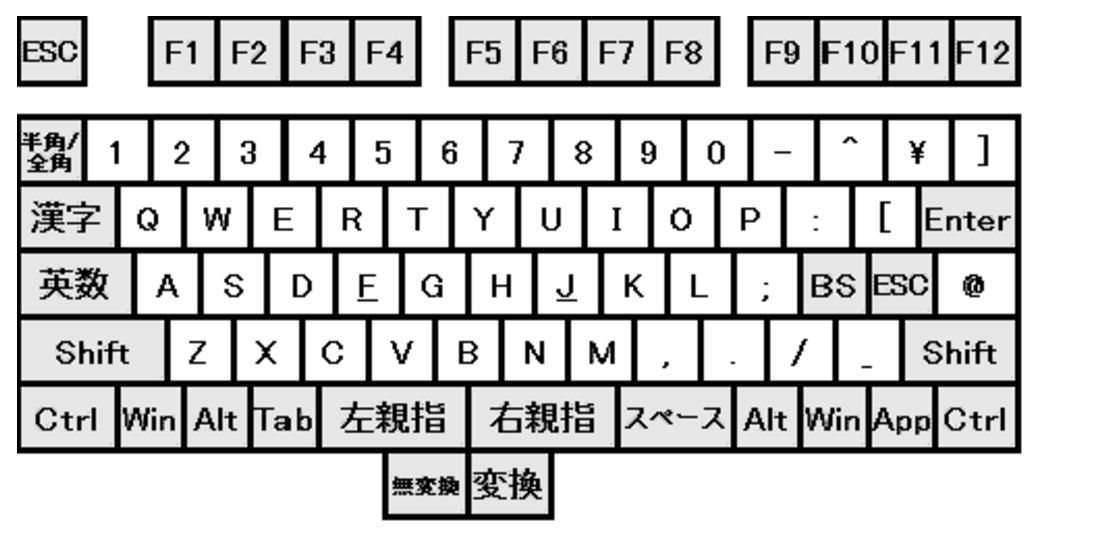
\includegraphics[width=14cm,clip]{res_kouy/oyayubi-shift_keyboard.eps}
 \end{center}
 \caption{�e�w�V�t�g�L�[�{�[�h}
 \label{oyayubi-shift_keyboard}
\end{figure*}

�ł��܂��e�w�V�t�g��������߂�K�v�͂���܂���B���݂ł͕��ʂ̃L�[�{�[�h���g���Đe�w�V�t�g�����邱�Ƃ��ł���̂ł��B�z��G�~�����[�^���g���΁A�L�[�{�[�h�̍ʼn��i�ɂ���\key{���ϊ�}�A\key{�X�y�[�X}�A\key{�ϊ�}�̂ǂꂩ2�L�[��e�w�L�[�Ƃ��āA���������e�w�V�t�g�L�[�{�[�h�̂悤�Ɏg�����Ƃ��ł��܂��B�Ⴆ�΁A\key{�X�y�[�X}��\key{���e�w}�A\key{�ϊ�}��\key{�E�e�w}�ł��邩�̂悤�Ɉ����āA�e�w�V�t�g���������邱�Ƃ��ł���̂ł��B

�u�e�w�L�[�ɂ����L�[�����X�̃L�[�̋@�\���g�������ꍇ�͂ǂ�����΂����̂��H�v�Ƃ����^�₪�킫�܂����A�G�~�����[�^�̕��Łu�����L�[�Ɠ����ɉ������ꍇ�̓V�t�g�L�[�Ƃ��āA�����L�[���������ɗ������ꍇ�͂��Ƃ��Ƃ̃L�[�Ƃ��āv�������Ă���܂��B�Ⴆ�΁A\key{�X�y�[�X}��\key{���e�w}�ɂ����ꍇ�ł��A\key{�X�y�[�X}��P�ɉ����ė������ꍇ�́A���ʂ�\key{�X�y�[�X}�����������̂Ƃ��Ĉ����Ă���܂��i���̂悤�ɂ��Ȃ��Őe�w�V�t�g��p�̃L�[�Ƃ��邱�Ƃ��ł��܂��j�B

�ǂ̃L�[��e�w�L�[�ɂ��邩�́A�����‚��̕��@������܂��B�s\key{�X�y�[�X}��\key{���e�w}�A\key{�ϊ�}��\key{�E�e�w}�t���s\key{���ϊ�}��\key{���e�w}�A\key{�ϊ�}��\key{�E�e�w}�t�ɂ���̂���ʓI�ł��B�|�C���g�ƂȂ�̂͐e�w�L�[�̈ʒu�ł��B�z�[���|�W�V�����Ɏw��u�����Ƃ��ɁA�e�w���u�e�w�L�[�v�̏�Ɏ��R�ɒu����̂����z�ł��B
�����L�[�Ɛe�w�L�[�𖳗��Ȃ������Ō��ł��邩�ǂ������d�v�ł��B���ɁA�e�w�L�[�Ɠ����ɉ����Ƃ��ɁA����ł�\key{Z}\key{T}\key{B}�A�E��ł�\key{Y}\key{N}\key{,}\key{.}\key{/}�������Ȃ������Ō��ł��邩���`�F�b�N���܂��傤�B

�܂��A�L�[�{�[�h�ɂ����\key{���ϊ�}�A\key{�X�y�[�X}�A\key{�ϊ�}�̈ʒu��傫���͂��Ȃ�قȂ�܂��B�L�[�{�[�h�͈������̂Ȃ�1000�`3000�~���x���甃���܂��̂ŁA�D�݂̐e�w�L�[�ɂȂ�悤�ȃL�[�{�[�h�ɕς��Ă݂�̂��ǂ��ł��傤�B

����ɁA��_�ȃL�[�{�[�h�����Ă�����܂��B�}\ref{migite_1retu_shift}�����Ă��������B\key{7}\key{Y}\key{H}\key{N}����E�̃L�[���A���ׂĉE��1��ړ����Ă��܂��B�{���Ȃ�\key{J}������ʒu��\key{H}���A\key{K}������ʒu��\key{J}���A�Ƃ����悤�ɉE�肪�S�����镶���L�[�����ׂĉE�Ɉ�񂸂�Ă���̂ł��i����ɁA�����L�[�̉E�[�̃L�[�������ɔz�u����Ă��܂��j�B������u�E����V�t�g�v�ƌĂт܂��B�L�[�J�X�^�}�C�Y�\�t�g���g���΁A���̂悤�ȉ������ȒP�Ɏ����ł��܂��B

�E����V�t�g�̍ő�̖ړI�́A�E��̃z�[���|�W�V�������E�Ɉړ����邱�Ƃł��B�z�[���|�W�V���������炵�Ă��e�w�������L�[�̈ʒu�͂��̂܂܂ł��B����ɂ��z�[���|�W�V�����Ɏw��u�����Ƃ��ɁA�E��e�w�����傤��\key{�ϊ�}�̏�ɗ���A�Ƃ����L�[�{�[�h������������̂ł��B�ꌩ�A�啝�ȕύX�Ȃ̂Ŋ����܂łɎ��Ԃ��|����悤�Ɏv���邩������܂��񂪁A�w�ƕ����L�[�̈ʒu�֌W�͕ς��Ȃ��̂ŁA�����Ɏg����悤�ɂȂ�܂��B�܂��A�E����V�t�g�Ɋ��ꂽ���ƂŒʏ�̃L�[�{�[�h���g���Ă��A���Ȃ��g�����Ƃ��ł��܂��B


\begin{figure*}
 \begin{center}
   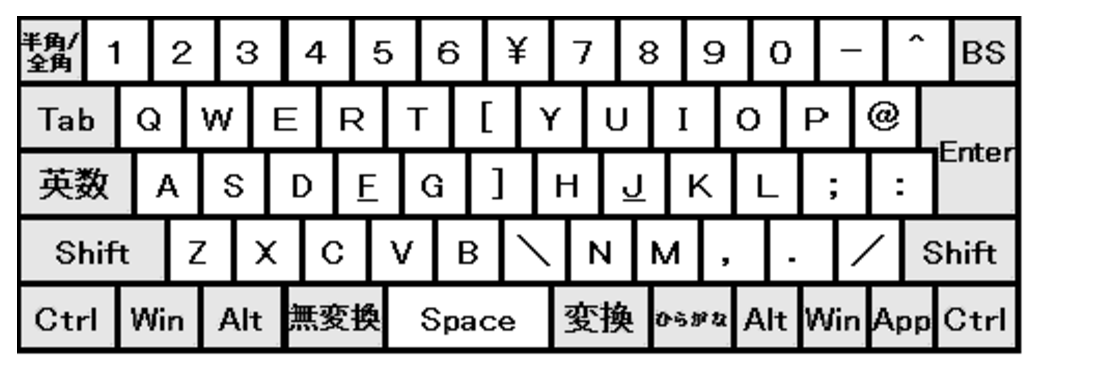
\includegraphics[width=14cm,clip]{res_kouy/migite_1retu_shift.eps}
 \end{center}
 \caption{�E����V�t�g}
 \label{migite_1retu_shift}
\end{figure*}

�������A�e�w�V�t�g�L�[�{�[�h���g�p����΁A�e�w�L�[�̈ʒu�Ƒ傫���͐\����������܂���B�{�i�I�ɐe�w�V�t�g���g�p���邱�Ƃɂ���Ȃ�A�e�w�V�t�g�L�[�{�[�h�̎g�p���I�����ɓ����Ă���ł��傤�B

\subsubsection*{BackSpace�̈ʒu�͑��}

������A�u�e�w�V�t�g�v�Ƃ͒��ڊ֌W�͂���܂��񂪁A�e�w�V�t�g�����͂��₷�����R�������܂��B

�e�w�V�t�g�ł́A�E�菬�w�z�[���|�W�V������1�‰E�̃L�[�A�‚܂�\key{:}�̈ʒu�̃L�[��\key{BackSpace}�����蓖�Ă��Ă��܂��B�ʏ�A\key{BackSpace}�͕����L�[�̉E��̊O��́A���Ȃ艓���ʒu�ɂ���܂��B�������A\key{BackSpace}�͕��͓��͂��s�����ōł��悭�g���L�[�̈�‚ł��B�ǂ�Ȃɏn�����Ă��^�C�v�~�X�𖳂����̂͗e�ՂȂ��Ƃł͂���܂���B�l���Ȃ��當�͂���͂���Ƃ��́A���ܓ��͂����������������ꍇ������܂��B���̂��тɉ�����\key{BackSpace}�������ɍs���Ƃ����̂͑�ςȘJ�͂ł��B\key{BackSpace}���߂��ɔz�u���邱�Ƃ́A�V�z��̎g�p�ɏ���Ƃ����Ȃ����͉��P���ʂ�����܂��B

�܂��A�V�z����K������Ƃ����_���猩�Ă��A\key{BackSpace}�������₷�����Ƃ͏d�v�ł��B�V�z�����K����ۂ́A�ǂ����Ă��^�C�v�~�X���������܂��B\key{BackSpace}�������₷���ʒu�ɂ���΁A�^�C�v�~�X�����Ă������ɏC���ł���̂ŁA�^�C�v�~�X�����ꂸ�ɂǂ�ǂ���͂��邱�Ƃ��ł��܂��B�ǂ�ǂ���͂ł���Α�������邱�Ƃ��ł��A�V�z��̏K���������Ȃ�܂��B

�e�w�V�t�g�ł́A\key{BackSpace}�̔z�u�ꏊ���A\key{:}�Ƃ����z�[���|�W�V��������߂��ʒu�Ɋm�ۂ���Ă��܂��B�e�w�V�t�g���g���ƁA�����I��\key{BackSpace}�������₷���ʒu�ɔz�u����邱�ƂȂ�܂��B����͐e�w�V�t�g�̉B�ꂽ�����b�g�ł��B

�e�w�V�t�g�ȊO�̔z��ł́A\key{BackSpace}�̈ʒu�͍l�����Ă��Ȃ����̂���������܂��B���{����͔z���\key{BackSpace}�̈ʒu���K�肷��Ƃ����̂��ςȘb�ł�����A���R�ƌ����Γ��R�ł��B�������A���܏������ʂ�\key{BackSpace}�̈ʒu�͓��{����͂ɂ����ĂƂĂ���؂ł��B\key{BackSpace}�̈ʒu�����߂��Ă��Ȃ��V�z����g���Ƃ��Ă��\�\�����ƌ����΁A�V�z����g�킸���[�}�����͂₩�ȓ��͂��g���Ƃ��Ă��\�\\key{BackSpace}��ł��₷���ꏊ�ɔz�u���邱�Ƃ��l���ėǂ��Ǝv���܂��B�Ⴆ�΁A�e�w�ɃV�t�g�L�[��z�u���Ȃ��z����g�p����Ȃ�A\key{���ϊ�}��\key{�ϊ�}�͐�D�̌��ƂȂ�܂��B

\subsection{���z��}

���z��́A���w�V�t�g�Ƃ����V�t�g�������g�p����z��ł��B�ʏ�̃V�t�g�L�[�i\key{Shift}�j�͕����L�[�̊O�́A���w�ʼn����ʒu�ɔz�u����Ă��܂��B�e�w�V�t�g�̃V�t�g�L�[�͐e�w�ʼn����ʒu�ɔz�u����Ă��܂����A�g�����L�[�̊O�ɔz�u����Ă���h�Ƃ����_�͒ʏ�̃V�t�g�L�[�Ɠ����ł��B����ɑ΂����w�V�t�g�ł́A��_�ɂ������L�[�̂ǐ^�񒆁A���Ȃ킿���w�̃z�[���|�W�V�����ł���\key{D}��\key{K}�ɃV�t�g�L�[��z�u���܂��B

�}\ref{tuki2-263}�͌��z��̔z��}�ł��B�e�L�[�̉��ɏ�����Ă��镶���͒P�łœ��͂���镶���ł��B����A��ɏ�����Ă��镶����\key{��}�̃L�[�i\key{D}��\key{K}�j�����O�ɉ����Ă����Ƃ��ɓ��͂���镶���ł��B�i�e�w�V�t�g�ƈقȂ�A���z��͓����Ō��ł͂���܂���B���Ƃŏڂ����������܂��j


\begin{figure*}
 \begin{center}
   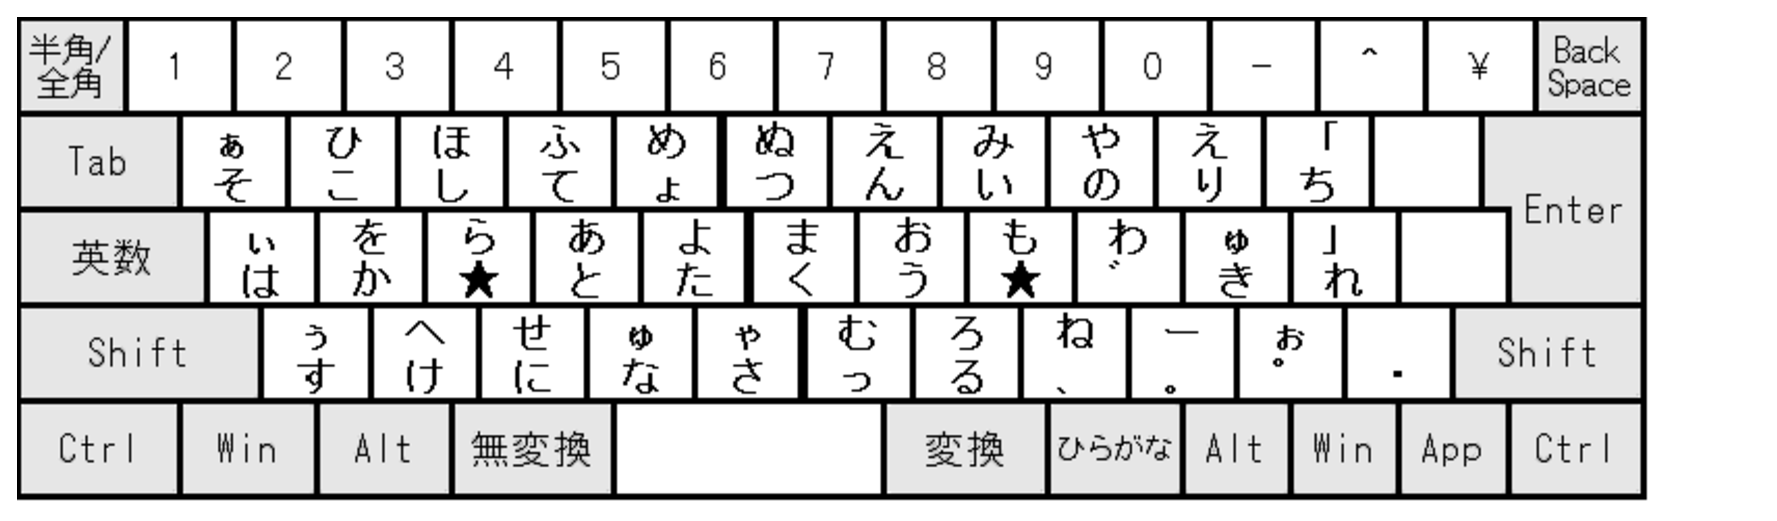
\includegraphics[width=14cm,clip]{res_kouy/tuki2-263.eps}
 \end{center}
 \caption{���z��2-263���z��}}
 \label{tuki2-263}
\end{figure*}

\subsubsection*{���w�V�t�g�̗��_}

���w�̃z�[���|�W�V�����ɃV�t�g��z�u���郁���b�g�́A���ł��傤���H

�܂��A�V�t�g�L�[����ʂȃL�[�ƍl����̂ł͂Ȃ��A�������͂Ɏg��1�‚̃L�[�ƂƂ炦�āA���̎g�p�����ǂꂭ�炢�ɂȂ邩���l���Ă݂܂��B

���{�����͂���ɂ�61��ނ̕�������͂���K�v������܂��i�L���Ȃǂ��܂߂�Ƃ����Ƒ����܂��j�B�܂��A�����̕������L�[�{�[�h�̏㒆���i�̂�����32�L�[���g�p���ē��͂��邱�Ƃɂ��܂��B1�‚̃L�[��1�‚̕�����z�u����̂ł́A�L�[�̐����S�R����܂���B�����ŁA2�‚̃L�[��g�ݍ��킹�ē��͂ł��镶���̎�ނ𑝂₷�u�V�t�g�v�Ƃ����V�X�e�����K�v�ɂȂ�܂��B

���ɁA�o�����̍������32��ނ̕������V�t�g�Ȃ��i�P�Łj�œ��͂��A�c��̕������V�t�g�L�[���g���ē��͂��邱�Ƃɂ��܂��B����Əo�����̒Ⴂ32�`61�ʂ̕����̍��v�o�����͖�16.1\%�ɂȂ�܂��B�‚܂�A���ꂾ���̉񐔃V�t�g�L�[�������K�v������킯�ł��B
�o�������ł����������́u�J�v�i���_�j�Ŗ�10.0\%�A2�ʂ��u���v�Ŗ�5.6\%�A3�ʂ��u���v�Ŗ�5.0\%�Ƒ����܂��B�V�t�g���g�p���镶���́A�����̃g�b�v�N���X�̏o�����̕����Ɣ�ׂĂ��������ŏo�����邱�Ƃ��킩��܂��B

���������āA�V�t�g�L�[����ʂȃL�[�ƍl�����A�u�悭�g���g�����h�͍ł������₷���ʒu�ɔz�u����v�Ƃ����ł��₷���z�������{�I�Ȕ��z�ɗ����čl����ƁA�ق��̂ǂ̕��������A�V�t�g�L�[�����A�ł��ǂ��ʒu�ɔz�u����ׂ����A�Ƃ������ƂɂȂ�܂��B�ł������₷���L�[�Ƃ��ẮA�l�����w�ƒ��w�̃z�[���|�W�V�������l�����܂��B�������A�l�����w�͂��Ƃ��ƒS���L�[�����i�㒆���i��3�i�Ɍ����Ă��j6�L�[�Ƒ������߁A�g�p�������܂�ɂ�����������^����̂ɂ͌����܂���B���������āA���w�̃z�[���|�W�V�����ł���\key{D}��\key{K}���V�t�g�L�[�̖������ʂ����̂ɍœK�ȃL�[�Ƃ������ƂɂȂ�܂��B

\subsubsection*{���z���������̂͒N���H}

���w�V�t�g�Ƃ������͕����́A�Ԕz��Ƃ����z��Œa�����܂����B1999�N�ɕy�~�땶�����l�Ă����z��ŁA�u���v�Ƃ��������ϊ��V�X�e���Ŏg�p���邱�Ƃ�z�肵�č���܂����B���w�V�t�g�����߂č̗p���A�R���s���[�^���g�p�����v�Z�ɂ�蕶���̔z�u�����肵���z��ł��B

�Ƃ���ŁA�VJIS�z��Ƃ����z�񂪂���܂��B1986�N�ɐ��肳�ꂽ�z��ŁA�]����JIS�z��i���ʂ̂��ȓ��͂̂��Ɓj�Ƃ͈قȂ�A�ŏ�i�i�����i�j�͎g�킸�㒆���i��3�i�ɂ��ׂĂ̕������z�u����Ă��܂��B���Z���ȏ���V���l��̃f�[�^���g�p���āA���E���ݑŌ��������A���w�ٌ������Ȃ��Ȃ�悤�ɍ���܂����B���ۂɐVJIS�z�񂪓��ڂ��ꂽ���[�v������������܂������A���y�͐i�܂��A1999�N�Ɂu�g�p���Ԃ��Ȃ����ߔp�~�v����܂����B

�VJIS�z����Ȃ��Ȃ��D�ꂽ�z�񂾂Ǝv���̂ł����A��–��m�Ȍ��_������܂����B����́A�ʏ�̏��w�ʼn����V�t�g�L�[���g�p���邱�Ƃł��i�Z���^�[�V�t�g���l������Ă��܂������A�������Ȃ������悤�ł��j�B�V�t�g�̎g�p���͏]���̂��ȓ��͂��������̂ŁA���w�ŃV�t�g�L�[�������Ə��w�̎g�p�������Ȃ荂���Ȃ��Ă��܂��̂ł��B

�u����Ȃ�VJIS�z��Œ��w�V�t�g���̗p����Ηǂ��̂ł͂Ȃ����H�v�A����Ȕ��z�����܂�܂����B�ǂ��Ő��܂ꂽ���Ƃ����ƁA���{�ő�̓d�q�f���A�Q�����˂�ł��B
2002�N�A�Q�����˂�̃p�\�R����ʔ‚Ɂu�y���[�}��,����,�e�w?�z�VJIS�z��L�[�{�[�h�v�Ƃ����X���b�h�������܂����B�����̘b��͐VJIS�z��̕]����g�p�@�ł������A�������ɑ��̔z��Ƃ̔�r�������悤�ɂȂ�A�Ԕz��̒��w�V�t�g���b��ɏオ��܂����B����ȗ���̒��Łu�w���w�VJIS�z��x�͂ǂ����H�v�ƒ�Ă��郌�X���������܂�܂��B�����Ď��ۂɒ��w�VJIS�z��������҂�����n�߁A����͂��񂾂�Ɛl���𑝂��Ă����A�������҂��獂�]���̃��X���������܂�܂��B

�₪�āA���w�VJIS�z��̈��̂Ƃ��āu���v����Ă���āA���̃X���b�h�̃^�C�g���́u�VJIS�E�� �L�[�{�[�h�z�� 2�Ō��ځv�Ɓu���v�Ƃ������̂����邱�ƂɂȂ�܂����B

�VJIS�z��͒��w�V�t�g�̂��߂ɍ��ꂽ�z��ł͂���܂���̂ŁA���̂܂ܒ��w�V�t�g�����邱�Ƃ͂ł��܂���B�VJIS�z��𒆎w�V�t�g�p�ɉ��ǂ���K�v������܂��B���ɁA�VJIS�z��Œ��w�̃z�[���|�W�V�����ɔz�u����Ă����������ǂ����邩�����ɂȂ�܂��B

�u�VJIS�z��̗ǂ����c�����܂ܒ��w�V�t�g������ɂ͂ǂ��z�u������ǂ����v�B�X���b�h���ł��܂��܂ȋc�_�����킳��A�����̉��LjĂ���Ă���܂����B�����Â��ɁA�ǂ���炱��ł��܂��������悤���Ƃ����z�񂪊������܂��B��������z��2-263���ƌĂт܂��B2-263�Ƃ����̂́A�VJIS�E���z��X���b�h��2�X���ڂ́A263�Ԃ̃��X�Œ�Ă��ꂽ�z��Ƃ����Ӗ��ł��B���̌�����ǂ͐i�߂��܂������A2-263���̈��p�҂͑����A2-263�������z��̍ł��W���I�Ȕz��Ƃ����ʒu�Â��ɂȂ��Ă��܂��B

���z��́A�VJIS�z��ƒ��w�V�t�g�Ƃ����g�ݍ��킹�̖����A�܂����o���Ă��܂��B�����āA���ꂪ���܂ꂽ�̂��C���^�[�l�b�g�̌f���‚ŁA�s���葽���̐l�̋��͂Ŋ��������Ƃ����_���ɂ߂Č��ݓI�ŁA�V�z��̏ے��ƌ����鑶�݂��Ǝv���̂ł��B

\subsubsection*{�G�~�����[�^�Ȃ�Ă���Ȃ��H}

���z��̒��w�V�t�g�́u�O�u�V�t�g�v�Ƃ����V�t�g�����œ��͂��܂��B�e�w�V�t�g�͓����Ō��ł������A���z��͓����Ō��ł͂���܂���B

�O�u�V�t�g�Ƃ����̂́A�u���̃L�[�������O�ɃV�t�g�L�[�������B�V�t�g�L�[�𗣂������ǂ����͖��Ȃ��v�Ƃ����V�t�g�����ł��B�Ⴆ�΁A���z��ŒP��\key{J}�������Ɓu���v�Ɠ��͂���܂����A���\key{D}�������Ă���\key{J}�������Ɓi\key{D}�𗣂������ǂ����͖��Ȃ��j�u���v�Ɠ��͂���܂��B

���̑�����Âɍl���Ă݂�ƁA�L�[�������^�C�~���O�̓��[�}�����͂Ɠ����ł��B���[�}�����͂ł��A�P��\key{A}�������Ɓu���v�Ɠ��͂���A\key{K}�������Ă���\key{A}�������Ɓu���v�Ɠ��͂���܂��B���z�������Ɠ������Ƃ����Ă��܂��B���������āA���z��͍��܂Ŏg���Ă������[�}�����͂ł̃L�[���������o�œ��͂ł���Ƃ��������b�g������܂��B

����ɁA�u���[�}�����͂Ɠ����V�X�e���ł���v�Ƃ������Ƃ���A�ӊO�ȃ����b�g�������܂��B����́uIME�̃��[�}���J�X�^�}�C�Y�Ŏ����ł���v�Ƃ������Ƃł��B���[�}���J�X�^�}�C�Y�Ƃ����̂́A���[�}���̂‚Â��ύX�ł���IME�̋@�\�ł��B�Ⴆ�΁A�ʏ탍�[�}�����͂ł�\key{K}�̎���\key{A}�������Ɓu���v�Ɠ��͂���܂��B����\key{K}��\key{A}�̕�����ύX�ł���̂ł��B���������āA\key{S}�������Ɓu���v�Ɠ��͂����悤�ɐݒ肷�邱�Ƃ��”\�Ȃ킯�ł��i�Ȃ��A�@�\�̖��̂�IME�ɂ���ĈقȂ�܂��B�wMicrosoft IME�x�ł́u���[�}���ݒ�v�A�wATOK�x�ł́u���[�}���J�X�^�}�C�Y�v�A�wGoogle ���{����́x�ł́u���[�}���e�[�u���v�Ƃ������̂ł��j�B

�V�z����g���ꍇ�̕s���_�̈�‚ɁA�u�����ł��邩�ǂ����v�Ƃ������̂�����܂��B�z��G�~�����[�^�Ŏ�������ꍇ�A���܎g���Ă���p�\�R���ŃG�~�����[�^�����Ғʂ�ɓ����Ȃ��”\��������܂��B�����̃p�\�R���ł͓����Ă��A�ʂ̃p�\�R���ł͓����Ȃ���������܂���B���͓����Ă����������Ȃ��Ȃ�Ƃ����s�������S�ɕ��@���邱�Ƃ͂ł��܂���B

���̓_�A���z��͂��Ȃ���S�ł��B�Ȃ��Ȃ�AIME�̃��[�}���J�X�^�}�C�Y�Ŏ������邱�Ƃ��ł��邩��ł��B���z��̃V�t�g�̃V�X�e���̓��[�}�����͂Ɠ����ł��̂ŁA���[�}���J�X�^�}�C�Y���g����IME�̋@�\�݂̂Ō��z��������ł��܂��B�G�~�����[�^���g���K�v������܂��񂩂�A�u�����ł��Ȃ��v�Ƃ����S�z�͂��Ȃ菭�Ȃ��Ȃ�܂��B

�������AIME�ɂ���Ă̓��[�}���J�X�^�}�C�Y�ɐ���������ꍇ������̂ŁA���z��̂��ׂĂ��������邱�Ƃ͂ł��Ȃ����Ƃ�����܂��B���̏ꍇ�AIME�p�ɏ����A�����W���Ď������邱�ƂɂȂ�܂��B�wGoogle ���{����́x�̃��[�}���J�X�^�}�C�Y�͔��ɋ��͂ł��̂ŁA�قڐ��������������邱�Ƃ��ł��܂��B

�܂��A�G�~�����[�^���g���ꍇ�ł����Ă��A�����Ō��Ȃǂ̕��G�ȑ��삪�Ȃ��̂ŁA�G�~�����[�^�̑I�����������A��������r�I�ȒP�ł��B�u���܂��܂Ȋ‹��ŐV�z����g�p�������v�u����G�~�����[�^�͎g�����Ȃ��Ȃ��v�Ǝv���l�ɂ��������߂ł��B

\subsection{AZIK}

���܂ŏЉ���u�e�w�V�t�g�v�Ɓu���z��v�́A���܂܂Ŏg���Ă������[�}�����͂Ƃ͂܂������ʂɁA�ꂩ�炩�Ȃ�z�u���������z��ł����B����ɑ΂��Ă��ꂩ��Љ��uAZIK�v�́A���܂Ŏg���Ă������[�}�����͂͂��̂܂ܐ������āA���̒��œ��͕��@�����P���悤�Ƃ����z��ł��B

\subsubsection*{���[�}�����͊g���z��Ƃ́H}

AZIK�́A���[�}�����͂��g�����āA���[�}�����͂ł͓��͂��ɂ������������P����z��ł��B

�Ⴆ�΁A���[�}�����͂Łu����v�Ɠ��͂���ꍇ��\key{S}\key{Y}\key{A}�Ɠ��͂��܂��B����͓�����O�̂��Ƃ̂悤�ł����A������\ruby{�X��}{�悤����}�̓��͂�3�Ō�������Ƃ����̂́A�����I�ł͂���܂���B�u����v��\key{J}\key{A}��2�Ō��œ��͂ł��邱�Ƃ��l����Ε�����悤�ɁA�X�����{����2�Ō��œ��͂ł��ėǂ��̂ł��B������AZIK�ł́A\key{X}�ł���s����͂ł��邱�Ƃɂ��܂��B�Ⴆ�΁A�u����v�Ɠ��͂���ꍇ��\key{X}\key{A}��2�Ō��œ��͂��܂��B����s�̝X���͂��Ȃ�o�����������̂ŁA���ꂾ���ł����\�ȓ��͉��P���ʂ�����܂��B

�ق��ɂ��AAZIK�ł͎��̂悤�Ȋg�����͂��g�p�ł��܂��B
\begin{itemize}
 \item \key{;}�i\key{L}��1�‰E�̃L�[�j�Łu���v����͂���B���[�}�����͂ł́u���v�̓��͕��@�́A�ꍇ�ɂ���Ďg���L�[���قȂ�ȂǕϑ��I�ł��B���̓��͕��@���g�����ƂŁA��ɕ�����₷�����͂��邱�Ƃ��ł��܂��B
 \item \key{C}�ł���s�̝X������͂���B�i��F\key{C}\key{A}�Łu����v�Ɠ��͂���j
 \item \key{Q}�Łu��v����͂���B���[�}�����͂ł́u��v�̓��͕��@�́A\key{N}�����œ��͂ł�����A\key{N}\key{N}�ȂǂƓ��͂��Ȃ���΂Ȃ�Ȃ��ꍇ���������肵�āA�ϑ��I�ł��B���̓��͕��@���g�����Ƃŏ��1�Ō��œ��͂��邱�Ƃ��ł��܂��B
 \item \key{:}�i\key{L}��2�‰E�̃L�[�j�Łu�[�v����͂���B�u�[�v�̓��[�}�����͂ŗB��ŏ�i���g�������ŁA���͂��Â炢�����ł��B������z�[���i�œ��͂ł���悤�ɂ��܂��B
\end{itemize}
AZIK�ł͂��̂悤�Ȋg�����͂�ςݏd�˂邱�ƂŁA���[�}�����͂����ł��₷���Ȃ�悤���P���Ă��܂��B

\subsubsection*{���[�}�����͂͂��̂܂܎g����}

AZIK�̊g�����͂̏d�v�ȓ_�́A���̂悤�ȉ��ǂ��d�˂Ă��A���Ƃ��Ƃ̃��[�}�����͂͂قڂ��̂܂܎g����Ƃ������Ƃł��B

�ŏ��ɁA\key{X}�ł���s�̝X������͂ł���Ə����܂����B�������A����́u����s�̝X������͂���Ƃ��͕K��\key{X}���g���v�Ƃ����Ӗ��ł͂���܂���B����\key{X}\key{A}�ł���s�̝X������͂ł��邱�Ƃ�Y��Ă��܂�����A�ʏ�ʂ�\key{S}\key{Y}\key{A}�Ɠ��͂��邱�Ƃ��ł��܂��B�܂��A\key{X}�Ƃ����L�[�́A���[�}�����͂ł͂قƂ�ǎg�p���܂���i�������̂��Ȃ̓��͂�\key{L}�ł��ł��܂��̂�\key{X}���g���K�v�͂���܂���j�B\key{X}�ł���s����͂ł��邱�Ƃɂ��Ă��A���Ƃ��Ƃ̃��[�}�����͂͂قڂ��̂܂܎g�p���邱�Ƃ��ł��܂��B

�ق���AZIK�̊g�����͂����Ă��A�u���v�̓��͂Ɏg��\key{;}�A�u��v�̓��͂Ɏg��\key{Q}�A�u�[�v�̓��͂Ɏg��\key{:}�ȂǁA���Ƃ��Ƃ̃��[�}�����͂ł͂قƂ�ǎg��Ȃ��L�[�΂���ł��B

���̂悤�ɁAAZIK�̊g�����͂́A�{���̃��[�}�����͂ł͎g��Ȃ��L�[��A�L�[�̑g�ݍ��킹���g���čs���܂��B���������āAAZIK������������Ԃł��AAZIK�̊g�����͂��܂������g�킸�A���[�}�����͂̂悤�ɓ��͂��邱�Ƃ��”\�ł��B���[�}�����͂��u�ύX�v���Ďg���₷������̂ł͂Ȃ��A�{���̃��[�}�����͂��u�g���v���邱�Ƃɂ���Ďg���₷������B���ꂪAZIK�̍ő�̓����ł��B

\subsubsection*{AZIK�̊o���₷��}

AZIK�̉��ǂ��u�g���v�ł��邱�Ƃ̃����b�g�́A���[�}�����͂��g�����܂܁A���͕��@�����P�ł��邱�Ƃł��B

�V�z����o���邱�Ƃœ��͌��������P���邱�Ƃ��ł��܂����A���͐V�z����o����܂ł̊��Ԃ��ǂ����邩�ł��B�ǂ�ȊȒP�Ȕz��ł��A�V�z����K������ɂ͂�����x�̗��K���Ԃ��K�v�ł��B�K���܂ł͕��͓��͂��܂Ƃ��ɂł��܂���B�V�z����g�������Ǝv���Ă��A���̊��Ԃ̂‚炳���v���Ă�����߂Ă��܂����������ł��傤�B

AZIK�Ȃ炻�̐S�z�͂���܂���BAZIK�Ȃ�A���܂Ŏg���Ă������[�}�����͂͂قڂ��̂܂܎g���܂��B���������āAAZIK�����S�ɏK�����Ă��Ȃ��i�K�ł��A�����Ɏ��ۂ̕��͓��͂Ŏg�p���邱�Ƃ��ł��܂��B�ł���͈͂Ŋg�����͂��g���A�Y��Ă��܂����烍�[�}�����͂̕��@�œ��͂���΂悢�̂ł��B��������Ďg���Ă��������Ɋ���Ċo���邱�Ƃ��ł��܂��B

�����āAAZIK�͊��S�Ƀ}�X�^�[����K�v���炠��܂���BAZIK�̊g�����͂́A��ɏЉ���ȊO�ɂ����܂��܂Ȃ��̂��p�ӂ���Ă��܂��B���ɂ͂��Ȃ荂�x�Ȋg��������܂��B�������AAZIK���g�p����̂ɂ�����g�����Ȃ��Ȃ���΂Ȃ�Ȃ��Ƃ������Ƃ͂���܂���B�u����s��\key{X}�œ��͂���v�u�u���v��\key{;}�œ��͂���v�Ƃ����ȒP�Ȋg�����͂������g���Ƃ����g�p���@�ł��ǂ��̂ł��B�ȒP�Ȋg�����܂��g���Ă݂āA����Ŋo�����鎩�M���‚����玟�̊g�����͂ɐi�ނ��Ƃ��ł��܂����A����ŏ\�����Ǝv���΂����܂ł̒i�K�Ŏg�������邱�Ƃ��ł��܂��B�����Ă��‚��]�T���ł�����A���߂Ď��̊g�����͂Ƀ`�������W����Ƃ������Ƃ��ł���̂ł��B

\subsection{Dvorak���[�}��}


\begin{figure*}
 \begin{center}
   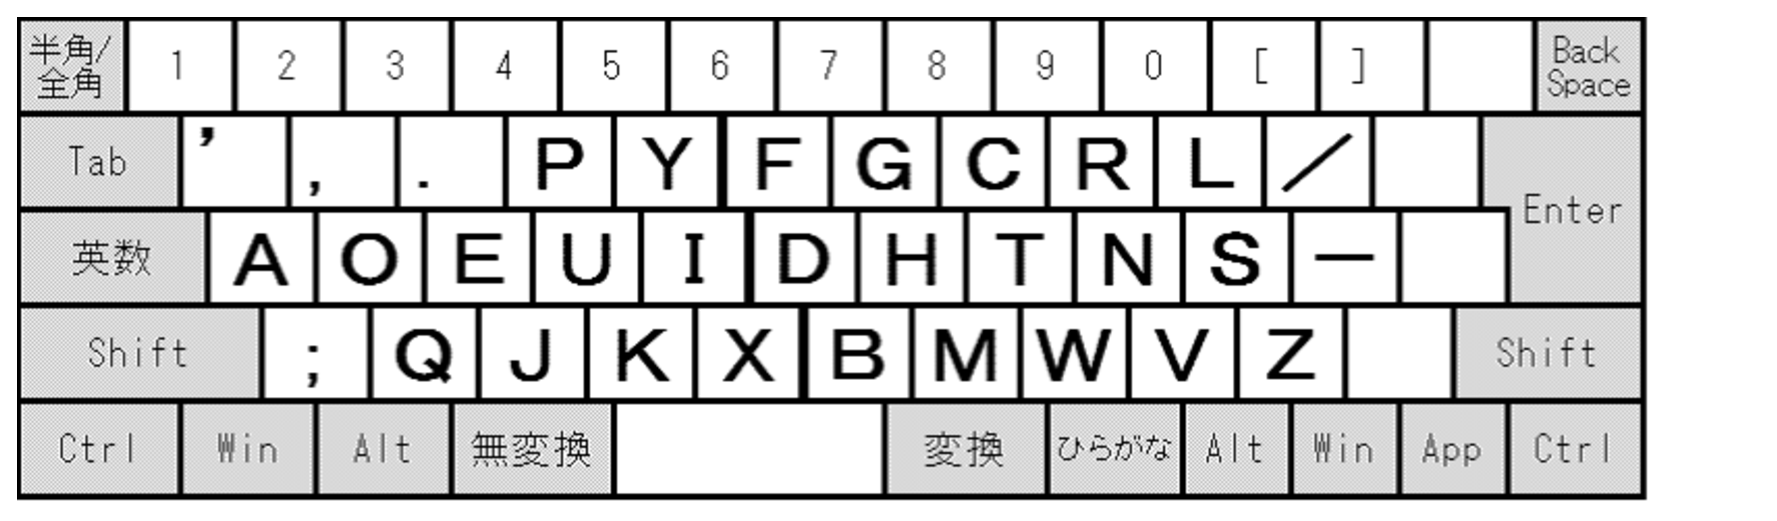
\includegraphics[width=14cm,clip]{res_kouy/Dvorak.eps}
 \end{center}
 \caption{Dvorak�z��}}
 \label{Dvorak}
\end{figure*}

\subsubsection*{�p����͂����P���悤}

����܂ŏЉ���V�z��́A���ׂāg���{��ł́h���͂����P���悤�Ƃ�����̂ł����B����A�p��ł����͕��@�����P���悤�Ƃ����z�񂪑��݂��܂��B��ʓI�ɑ����g���Ă���A���t�@�x�b�g�̔z��̂��Ƃ��A�L�[�{�[�h�̏�i�̍�����6����������āuQwerty�z��v�ƌĂт܂��BQwerty�z��ɑ���z��Ƃ��ėL���Ȃ̂��uDvorak�z��v�ł��B

Dvorak�z��̐��藧���͌Â��A1932�N�ɃA�����J�Ő��܂�܂����B�l�Ď҂̃I�[�K�X�g�E�h���H���b�N���O�������Dvorak�z��ƌĂ΂�Ă��܂��B�p���ł̃A���t�@�x�b�g�̏o������L�[�̑ł��₷�����l�����Ċe�����̔z�u�����߂��Ă��܂��B�ꉹ�����ׂč���̃z�[���i�ɔz�u����Ă���̂������BQwerty�z��ɔ�ׂČ��ݑŌ����������A�w�̈ړ��������Z���Ȃ�܂��B�^�C�s���O���x����K���̌���A\ruby{�F�≊}{���񂵂傤����}�Ȃǂ̖h�~�Ɍ��ʂ�����ƌ����Ă��܂��B

���́ADvorak�z��̓��[�}�����͂�����ꍇ���D�ꂽ�z��ł��B�Ƃ����̂́ADvorak�z��̓��[�}�����͂̕ꉹ�ł���\key{A}\key{I}\key{U}\key{E}\key{O}������̃z�[���i�ɕ��ׂĔz�u����Ă��邩��ł��BQWERTY�z��̃��[�}�����͂̌��_�́A�ł��悭�g���L�[�ł���ꉹ�L�[���A�ł��ł��₷���ꏊ�ɂ͔z�u����Ă��Ȃ����Ƃł����B\key{A}�����w�̃z�[���|�W�V�����ɂ��邾���ŁA�ق���4�L�[�͂��ׂăz�[���i����O�ꂽ�ꏊ�ɂ���܂��BDvorak�z��Ȃ�ꉹ�����ׂăz�[���i�ɂ���܂��B���������ĕꉹ����͂���Ƃ��Ƀz�[���|�W�V��������w������ɂ����A�����I�ɓ��͂��邱�Ƃ��ł��܂��B

���{��̓��͂ƂƂ��ɉp��̓��͂����P�������Ƃ������́ADvorak�z����o���ė�����C�ɂ���ʼn�������Ƃ����̂��ǂ��Ǝv���܂��B

\subsubsection*{Dvorak���[�}�����g�����悤}

�������A���R�Ȃ���Dvorak�����[�}�����͗p�ɍ��ꂽ�z��ł͂���܂���̂ŁADvorak�z��ł��̂܂܃��[�}�����͂����悤�Ƃ���ƁA�����‚��C�ɂȂ�_���o�Ă��܂��B
��\�I�Ȃ̂��A\key{K}���ꉹ�Ɠ������葤�ɂ��邱�Ƃł��B���̂��߁A���s�̂��Ȃ���͂��邽�тɍ���𑱂��Ďg�����ƂɂȂ�܂��B���ɁA�u���v�Ɓu���v����͂���Ƃ��ɍ���̐l�����w�𑱂��Ďg�����ƂɂȂ�̂����ł��B

���̖��̉�����Ƃ��ėL���Ȃ̂́A���s�̓��͂�\key{K}�̑����\key{C}�łł��邱�Ƃɂ���Ƃ������@�ł��B���o�I�ɂ��ACA�Łu���v�Ɠǂ߂܂����ACA�ECU�ECO�Łu���E���E���v�Ɠ��͂ł���IME�������ł��B�����Ζ��Ȃ����͂ł���ł��傤�B

����ɉ��Ǔ_���g�債�āAAZIK�̂悤�Ȋg�����[�}�����͂�Dvorak�z��ɂقǂ������z�������܂��B�wDvorakJP�x�͔�r�I���₩�ȉ��ǁB����Dvorak�z�񂩂�ύX�_�����Ȃ��A�Ȃ��݂₷���Ǝv���܂��B�wACT�x�͓��ݍ��񂾉��ǁB�uAZIK�v�Ɠ����悤�ɊȒP�Ȋg�����獂�x�Ȋg���܂ŕ��L�������A�ł��ɂ����^�w���ł������Ȃ�����_�ȉ��ǂ��{���Ă��܂��B

������Dvorak�g���z��́A���ɂ��Ă���Dvorak�z�񎩑̂����[�}�����͂ɓK���Ă���̂ŁA�p��z��𗣂�āA�P�ɓ��{����͔z��Ƃ��Č��Ă����Ȃ苭�͂ł��B��������Dvorak�z����o����̂Ȃ�A���{����͂̕��͍ŏ�����Dvorak�g���z����o����Ƃ����̂��ǂ��ł��傤�B

\subsection{�����Ȃ��}


\begin{figure*}
 \begin{center}
   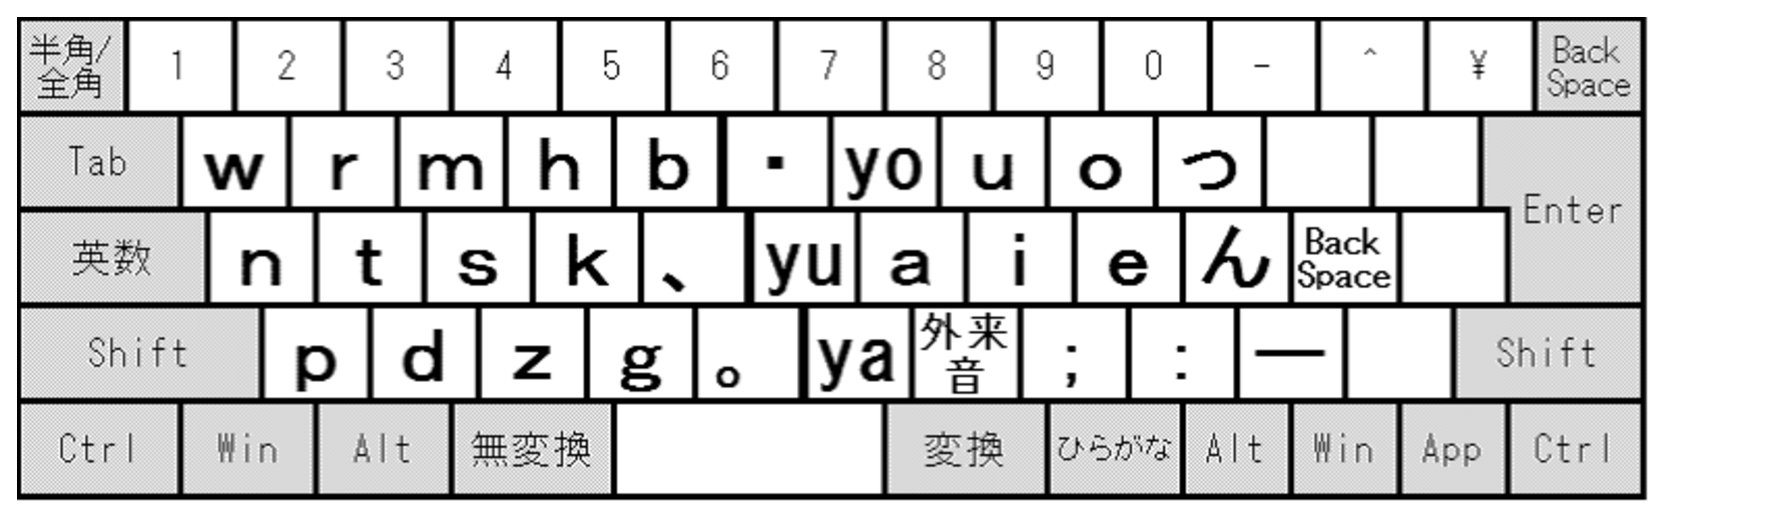
\includegraphics[width=14cm,clip]{res_kouy/keinarabe.eps}
 \end{center}
 \caption{�����Ȃ�הz��}}
 \label{keinarabe}
\end{figure*}

\subsubsection*{�܏\�����s�i�n�z��}

�����Ȃ�ׂ́A�o���₷���ɏd�_���������s�i�n�z��ł��B�s�i�n�Ƃ����̂́A1�‚̕�������{�I�Ɏq���ƕꉹ��2�Ō��œ��͂���z��̂��Ƃł��B���Ȃ̌܏\���\�𗘗p���āA�q���ƕꉹ��g�ݍ��킹�邱�Ƃ�1�‚̂��Ȃ���͂��܂��B���[�}�����͂��s�i�n�z��̈��ł��B

�����āA�����Ȃ�ׂł͎q���ƕꉹ�����E�ɂ͂����蕪����Ĕz�u����Ă��܂��i�}\ref{keinarabe}�j�B���肪�q���L�[�S���A�E��ɕꉹ�L�[�S���ł��B

����ɁA���̃L�[�̕��ѕ������Ȃ�K���I�ł��B�q������͂���L�[�͍���l�����w�̃z�[���|�W�V�����ł���\key{F}���N�_�Ƃ��āA�������獶�ɂ��s�A���s�A���s�A�ȍs�̏��ԁB��i�Ɉڂ���\key{R}����͍s�A�܍s�A��s�A��s�̏��ԂƂȂ��Ă��܂��B����͂��Ȃ��݂̌܏\�����Ɠ������Ԃł��i�Ȃ��A�����Ȃ�ׂł͂�s�̎q���L�[�͂���܂���B���Ƃŏڂ����������܂��j�B����ɑ�������͂���L�[���A���s�A���s�A���s�̃L�[�́A���̐����̃L�[�̂������ɔz�u����Ă��܂��B�ꉹ���A���ϑ��I�ł͂���܂����A�E��̃z�[���|�W�V�����ł���\key{J}���N�_�Ƃ��Ă������������ŕ��ׂ��Ă��܂��B

���̂悤�ɁA�����Ȃ�ׂł͂Ȃ��ݐ[���܏\���̏��Ԃ𗘗p���Ċo������悤�ɍ���Ă��܂��B����Ȃ炷���ɂł��o���邱�Ƃ��ł���ł��傤�B

\subsubsection*{���E���ݑŌ��ƃA���y�W�I�̈З�}

�u�m���ɂق��̔z����o���₷�����ł͂��邯�ǁA�s�i�n�Ƃ������Ƃ͊�{�I��1�‚̂��Ȃ̓��͂�2�Ō�������B����ł͏K�����Ă��\���ȓ��͉��P���ʂ͓����Ȃ��̂ł́H�v�Ǝv���������邩������܂���B�m���ɁA�����Ȃ�ׂ̑Ō����́A���[�}�����͂��͏��Ȃ����̂́A1�Ō���1�������͂ł��邩�Ȍn�̔z��Ɣ�ׂ�Ƃ��Ȃ葽���Ȃ�܂��B�Ō���������Ȃ��̂ł͉��P���ʂ��債�����Ƃ͂Ȃ����낤�A�ƍ����������邩������܂���B�������A�����Ȃ�ׂ́A���͌������P���ʂ������ĕ��邱�Ƃ͂ł��Ȃ��̂ł��B

�����Ȃ�ׂ����͂��₷�����̗��R�́A��{�I�ɍ��E���ݑŌ��œ��͂ł��邱�Ƃł��B
���E���ݑŌ��Ƃ����̂́A����ŃL�[��ł����玟�͉E��A�E��ŃL�[��ł����玟�͍���Ƃ����悤�ɁA���E�̎�����݂Ɏg���đŌ����邱�Ƃł��B����͓��͂��₷�����͕��@�ł��B�Ȃ��Ȃ�A����̎�ŃL�[��ł��Ă���ԂɁA��������̎�̓L�[���������������邱�Ƃ��ł��邩��ł��B

�����Ȃ�ׂł͎q��������ŁA�ꉹ���E��œ��͂��܂��B�s�i�n�̓��͕��@�ł͊�{�I�Ɏq���ƕꉹ�����݂ɏo�Ă��܂��̂ŁA�K�R�I�ɍ��E���ݑŌ��œ��͂ł���̂ł��B

�������A���E���ݑŌ��ł͓��͂ł��Ȃ�����������܂��B�Ⴆ�΁A�A�ꉹ�̕����ł��B�A�ꉹ�Ƃ����̂́A���[�}���ŕꉹ���A�����ďo�����镔���̂��Ƃł��B�Ⴆ�΁A�u�����v�Ƃ�����������͂���Ƃ���\key{K}\key{A}\key{I}�Ɠ��͂��܂��B�ꉹ��A��I���A�����Ă��܂�����A���̕����͘A�ꉹ�Ƃ������ƂɂȂ�܂��B�����Ȃ�ׂ̕ꉹ�͂��ׂĉE��œ��͂��܂�����A�A�ꉹ�̕����͕K�R�I�ɓ�����𑱂��Ďg�����ƂɂȂ�܂��B

�������A�ނ��낱�̘A�ꉹ�������A�����Ȃ�ׂ̓��͂��₷���̐^�����Ƃ����镔���ł��B���̔閧�́A�A�ꉹ�̕΂�ƁA�A�ꉹ���A���y�W�I�œ��͂ł��邱�Ƃł��B

�A�ꉹ�̏o�����́A���Ȃ̏o�����Ɠ����悤�ɂɑ傫�ȕ΂肪����܂��B�ꉹ��5��ނł�����A�A�ꉹ�͑S����25��ނ���܂��B���̂����o�����̍���ai�Aei�Aou��3��ނ̘A�ꉹ�őS�̖̂�55.3\%���߂܂��B����3��ނ̘A�ꉹ�����ɏo���Ă݂�ƁA�����g�����ł��邱�Ƃ���������Ǝv���܂��B���Ɋ����̉��ǂ݂ő����g���܂��B

�����Ȃ�ׂł́A���̏o�����̍���3�‚̘A�ꉹ���A���y�W�I�œ��͂ł���悤�ɂ��Ă���܂��B�A���y�W�I�Ƃ����̂́A�u�Е��̎�ő����ăL�[�������ꍇ�ɁA���ɉ����₷���A�ځv�̂��Ƃł��B�Ⴆ��\key{K}��\key{J}�ƑŌ�����ꍇ���A���y�W�I�ł��B���ۂɃL�[�������Ă݂�ƁA����2�L�[��Ō�����ꍇ�͑����y�ɑŌ��ł��邱�Ƃ���������Ǝv���܂��B�����Ȃ�ׂł́A�A�ꉹai��\key{J}��\key{K}�Aei��\key{L}��\key{K}�Aou��\key{O}��\key{I}�ƁA���ׂăA���y�W�I�œ��͂ł���悤�ɔz�u���Ă���܂��B�����Ȃ�ׂ̕ꉹ�́A�q���ɔ�ׂ�Ƃ��ϑ��I�ȏ��Ԃŕ���ł��܂����A����͘A�ꉹ���A���y�W�I�őłĂ�悤�ɂ��邽�߂ł��B

��{�͍��E���ݑŌ��A�o�����̍����A�ꉹ�̓A���y�W�I�œ��́B����2�‚̍H�v�ɂ��A�����Ȃ�ׂ͊o���₷���܏\�����z��ł���Ȃ���A�������͉��P���ʂ��������Ă��܂��B

\subsubsection*{����̕ꉹ���Ƃ́H}

�����ЂƂA�����Ȃ�ׂ̑傫�ȓ���������܂��B����́A�u����v��ꉹ�����Ĉ����Ă��邱�Ƃł��B

�ʏ�̃��[�}�����͂ł́A�ꉹ�́uaiueo�v��5��ނł��B�ua�v�͒P�łŁu���v����͂��܂��B�q���uk�v�ƕꉹ�ua�v�̑g�ݍ��킹�Łu���v����͂��܂��B�u����v��ꉹ������Ƃ����̂́A�uya�Ayu�Ayo�v���ua�Ai�Au�Ae�Ao�v�Ɠ��������ɂ���Ƃ������Ƃł��B���������āA�uya�Ayu�Ayo�v��P�łœ��͂ł���L�[�����݂��܂��B�����Ȃ�הz��}�i�}5-6�j��\key{N}\key{H}\key{U}�̃L�[�A�����珇�ԂɁuya�v�uyu�v�uyo�v�ƕ���ł��镔��������ł��B�����̃L�[��P�łʼn����ƁA�u����v�����͂���܂��B����A�q���L�[����������Ɂuya�Ayu�Ayo�v�������ƁA�X������͂��܂��B�Ⴆ�΁A�uk�v�̃L�[�������Ă���uya�v�̃L�[�������Ɓu����v����͂��܂��B�X���Ƃ����̂́A�q���Ƃ�s�̑g�ݍ��킹�ł��ׂĕ\�����邱�Ƃ��ł���̂ł��B

�}\ref{keinarabe_50on}�͂����ꉹ���������܏\���\�ł��B�����ꉹ��������Ƃ����Ɗ�قɎv���邩������܂��񂪁A�\�����ԂȂ����߂���ŝX�����K���I�Ɏ�荞�߂�̂ŁA�ނ���ʏ�̌܏\���\��蕪����₷���܂Ƃ܂��Ă���Ǝv���܂��B


\begin{figure*}
 \begin{center}
   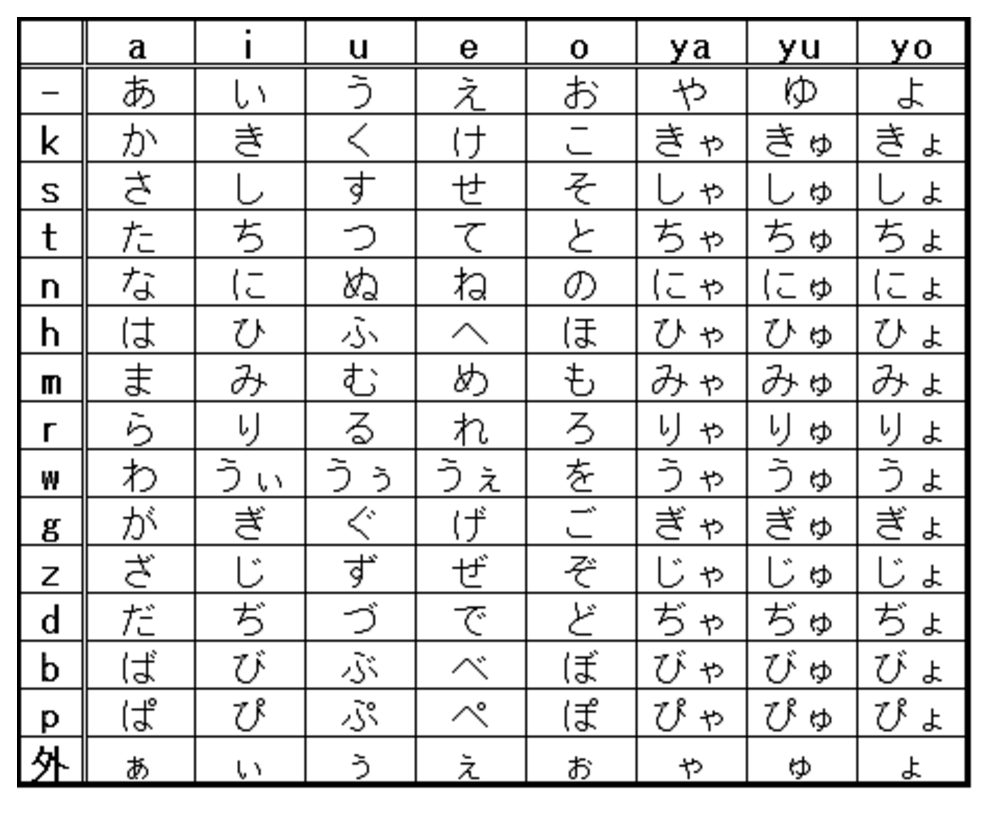
\includegraphics[width=14cm,clip]{res_kouy/keinarabe_50on.eps}
 \end{center}
 \caption{�����ꉹ���������܏\���\}
 \label{keinarabe_50on}
\end{figure*}

�����ꉹ�����郁���b�g��2�‚���܂��A�܂��A�X�������ׂ�2�Ō��œ��͂ł��邱�Ƃł��B�ʏ�̃��[�}�����͂ł͝X���̓��͂͑�����3�Ō��ł��̂ŁA���̕��Ō��������炷���Ƃ��ł��܂��B�ʏ�̃��[�}�����͂ł��A����s�̝X��������2�Ō��œ��͂ł���̂ŁA����s�����͓��͂��₷���Ɗ������Ă�����������Ǝv���܂��B���ꂪ���ׂĂ̝X���Ɋg�傳���̂͑傫�ȃ����b�g�ł��B

������‚́A��s�̘A�ꉹ�̓��͂����₷�����Ƃł��B��قǕp�o����A�ꉹ��ai�Aei�Aou��3�‹����܂����B�������A���͂����ꉹ�������邱�Ƃɂ���ƁAyou�i�傤�j�Ƃ����A�ꉹ�����ɂ悭�o������A�ꉹ�ƂȂ�܂��B�u�傤�v�Ƃ��������̘A�Ȃ�́A2�����̘A�Ȃ�̒��ł͒f�g�c�ł��B�����Ȃ�ׂł́A���̘A�ꉹyou��\key{U}��\key{I}�̃A���y�W�I�œ��͂ł���悤�ɂȂ��Ă��܂��B�u����v���i�ォ��ł͂Ȃ��j�����珇�Ԃɕ���ł���̂́A\key{yo}��\key{u}���A���y�W�I�œ��͂ł���悤�ɂ��邽�߂ł��B

�ʏ�̘A�ꉹ3��ɉ����āA�X���̘A�ꉹyou���A���y�W�I�œ��͂ł��邱�Ƃɂ��A�����Ȃ�ׂ͍s�i�n�̓��͕��@�ł���Ȃ���A�Ō������ӎ������Ȃ��X�s�[�h���̂�����͂����邱�Ƃ��ł���̂ł��B


\clearpage
\articlepart{�������̂��߂̔z��K��}{tomoemon}

\section{�͂��߂�}

�u��葬�����͂ł���悤�ɂȂ肽���v�Ƃ����̂͋��Z�^�C�s���O�Ɏ��g�ސl�Ȃ�N�����v�����Ƃł��B�����ł‚��߂̕��@�_����K�@�ɂ‚��Ă͖{���̑��̋L���ɂ��ڂ��Ă��܂����A���̋L���ł́u�ŏ��Ɋo�����L�[�{�[�h�z��Ƃ͕ʂ̔z��v���K�����č����ȃ^�C�s���O��ڎw�����@�ɂ‚��ďЉ�Ȃ���A���̕��@�̗ǂ��_�A�����_���l���Ă����܂��B

�����ł����u�ŏ��Ɋo�����L�[�{�[�h�z��Ƃ͕ʂ̔z��v�Ƃ́A�Ⴆ�΃��[�}�����͂��ŏ��Ɋo�����l�ɂƂ��Ă̂��ȓ��͂�A���ȓ��͂��ŏ��Ɋo�����l�ɂƂ��Ẵ��[�}�����͂����Ă͂܂�܂��B������񂱂�ȊO�ɂ��AQwerty�z�񂩂�Dvorak�z��ɏ�芷����A�e�w�V�t�g�z��ɏ�芷����Ƃ������l�X�ȏꍇ���l�����܂��B�ǂ̂悤�ȃp�^�[���ɂ���A����̔z��ɉ��炩�̌��E�������āA����ȊO�̔z��ɉ”\�����������Ƃ��ɏ�芷���邱�Ƃ������Ǝv���܂��B�����ł͓��ɓ��͑��x�̌��E�A�”\���Ƃ����ϓ_�ł��̕��@�̗L�����ɂ‚��čl���Ă����܂��B

\section{�p��̊m�F}

\subsection{�L�[�{�[�h�z��}

�u�L�[�{�[�h�z��i���邢�͒P�ɔz��j�v�Ƃ������t�̈Ӗ��ō������邱�Ƃ�����̂Ő�ɐ������Ă����܂��B��ʓI�ɃL�[�{�[�h�z��Ƃ����ƃL�[�{�[�h�Ɉ󎚂���Ă���\key{Q}\key{W}\key{E}\key{R}\key{T}\key{Y}�Ƃ������т̂��Ƃ��C���[�W����Ǝv���܂����A��̂���Ŗ�肠��܂���B�Ⴆ�ΐ}\ref{qwerty}��Qwerty�z��ƌĂ΂����̂Ō��ݍL�����y���Ă�����̂ł��B


\begin{figure*}
 \begin{center}
   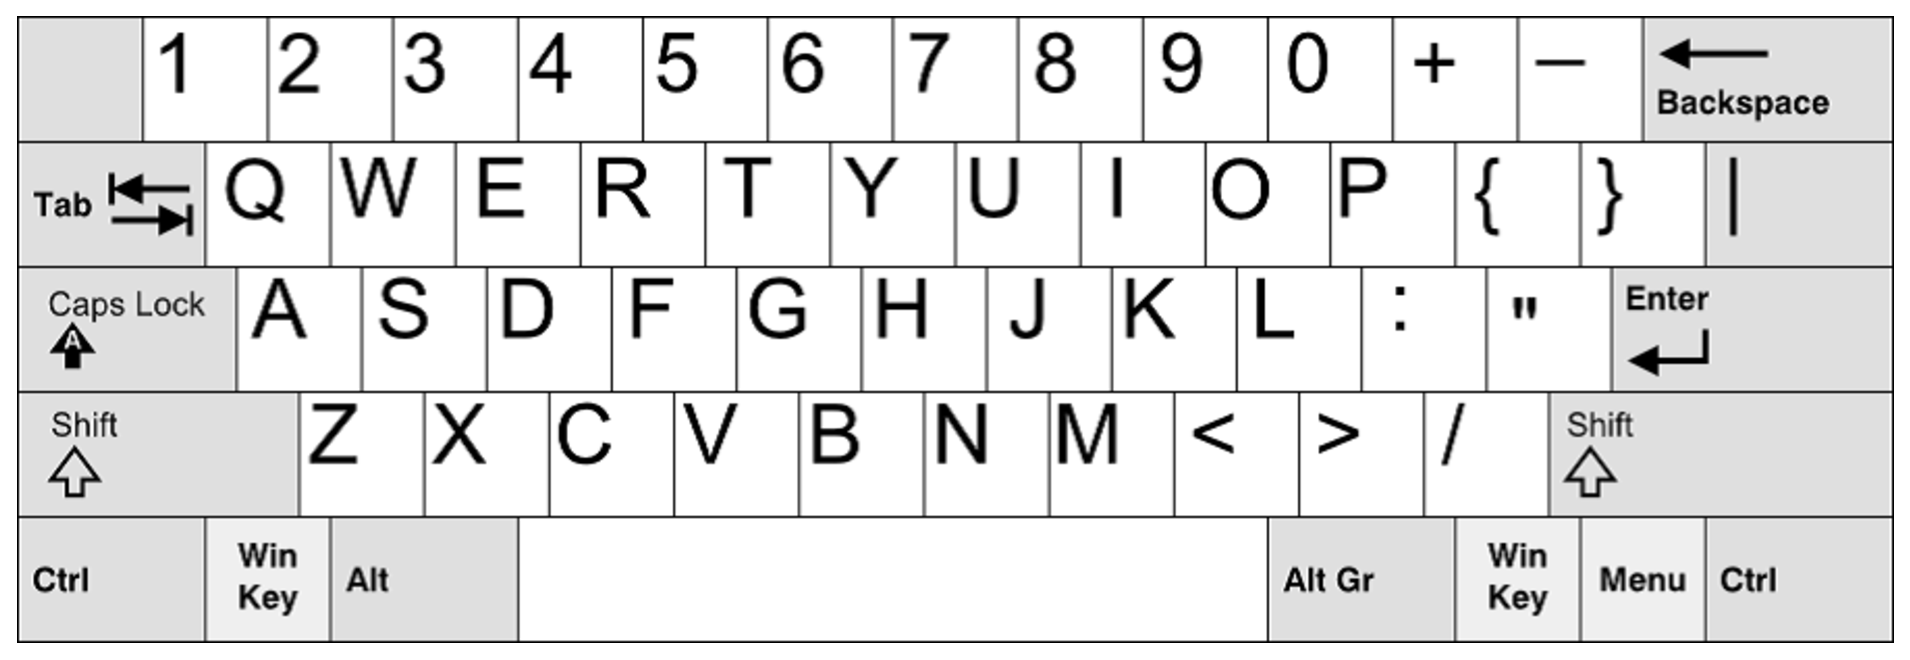
\includegraphics[width=14cm,clip]{res_tomoemon/qwerty.eps}
 \end{center}
 \caption{Qwerty�z��}
 \label{qwerty}
\end{figure*}

���̔z����g���ĉp�����̓��[�h��\key{Q}��������[q]�Ƃ����������R���s���[�^�ɓ��͂���܂��B�ǂ̃L�[���������Ƃ��ɉ��̕��������͂���邩�A�Ƃ����g�ݍ��킹���L�[�{�[�h�̘_���z��ƌ����A���̋L���Ŕz��ƌ������ꍇ�͂�����w���܂��B����A�����I�ȃL�[�̌`���ʒu���L�[�{�[�h�̕����z��ƌ����܂��B���݂̃L�[�{�[�h�̑����͊e�i�̃L�[�̈ʒu���������‰��ɂ���Ă��܂����A���ꂢ�Ȋi�q��ɂȂ��Ă��镨���z��̃L�[�{�[�h�����݂��܂��B

�����z��Ƙ_���z��̃C���[�W���킫�ɂ������͖����󃂃f���L�[�{�[�h\footnote{\url{http://www.pfu.fujitsu.com/hhkeyboard/hhkbpro2/nokeytop.html}}���C���[�W����Ɨǂ��ł��傤�B

\begin{figure*}
 \begin{center}
   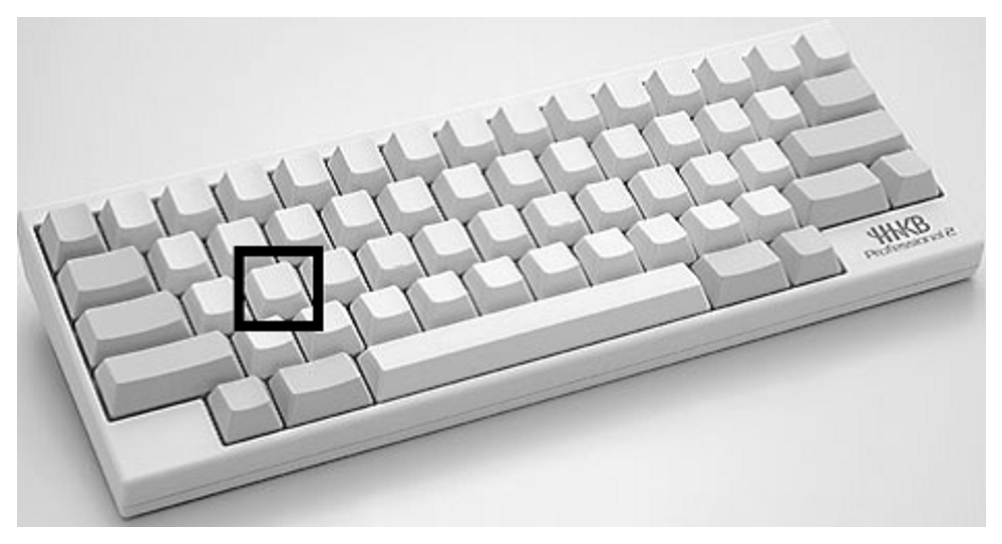
\includegraphics[width=14cm,clip]{res_tomoemon/nokeytop.eps}
 \end{center}
 \caption{Happy Hacking Keyboard Professional2 ���^������}
 \label{nokeytop}
\end{figure*}


�}\ref{nokeytop}�Ŏl�p���g�ň͂񂾈ʒu�̃L�[���������Ƃ��ɉ��̕������o�邩�͘_���z��ɂ���Č��܂�܂��BQwerty�z����g���Ă����[s]���o�܂����A�}\ref{dvorak}��Dvorak�z��ł�[o]�̕������o�܂��B

\begin{figure*}
 \begin{center}
   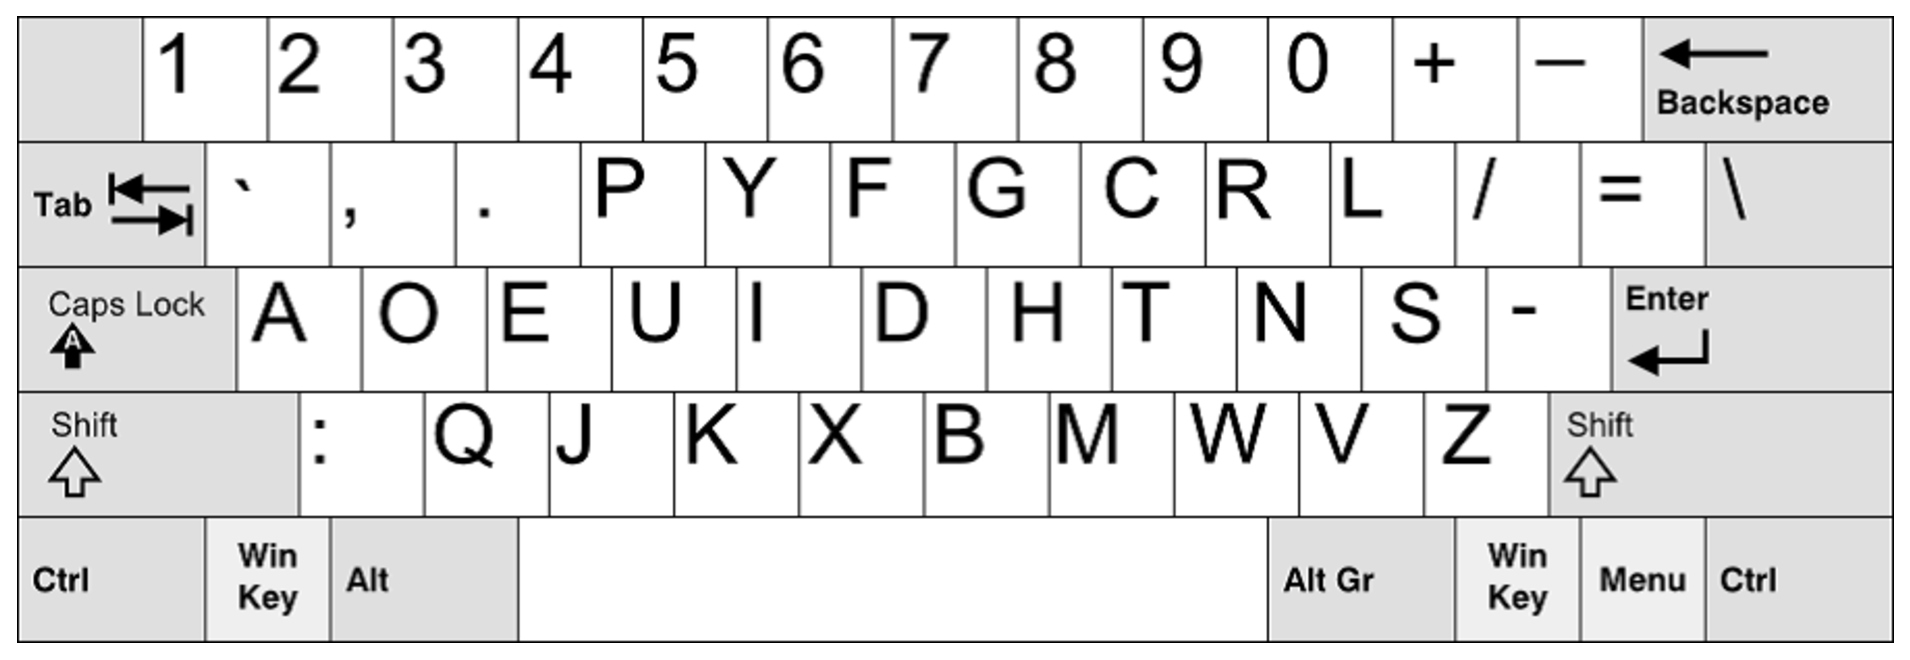
\includegraphics[width=14cm,clip]{res_tomoemon/dvorak.eps}
 \end{center}
 \caption{Dvorak�z��}
 \label{dvorak}
\end{figure*}

�����z��̏�ɂ͂����‚��_���z����d�˂邱�Ƃ��ł��A�Ⴆ�Ε����I�ȃL�[�{�[�h1���ŁAQwerty�̉p�����́A���ȓ��́A���[�}�����͂Ƃ����������̔z���؂�ւ��A�܂��͑g�ݍ��킹�Ď������邱�Ƃ��ł��܂��B�}\ref{arrangement}�͕����z��Ƙ_���z��̊֌W��\�������̂ł��B

\begin{figure*}
 \begin{center}
   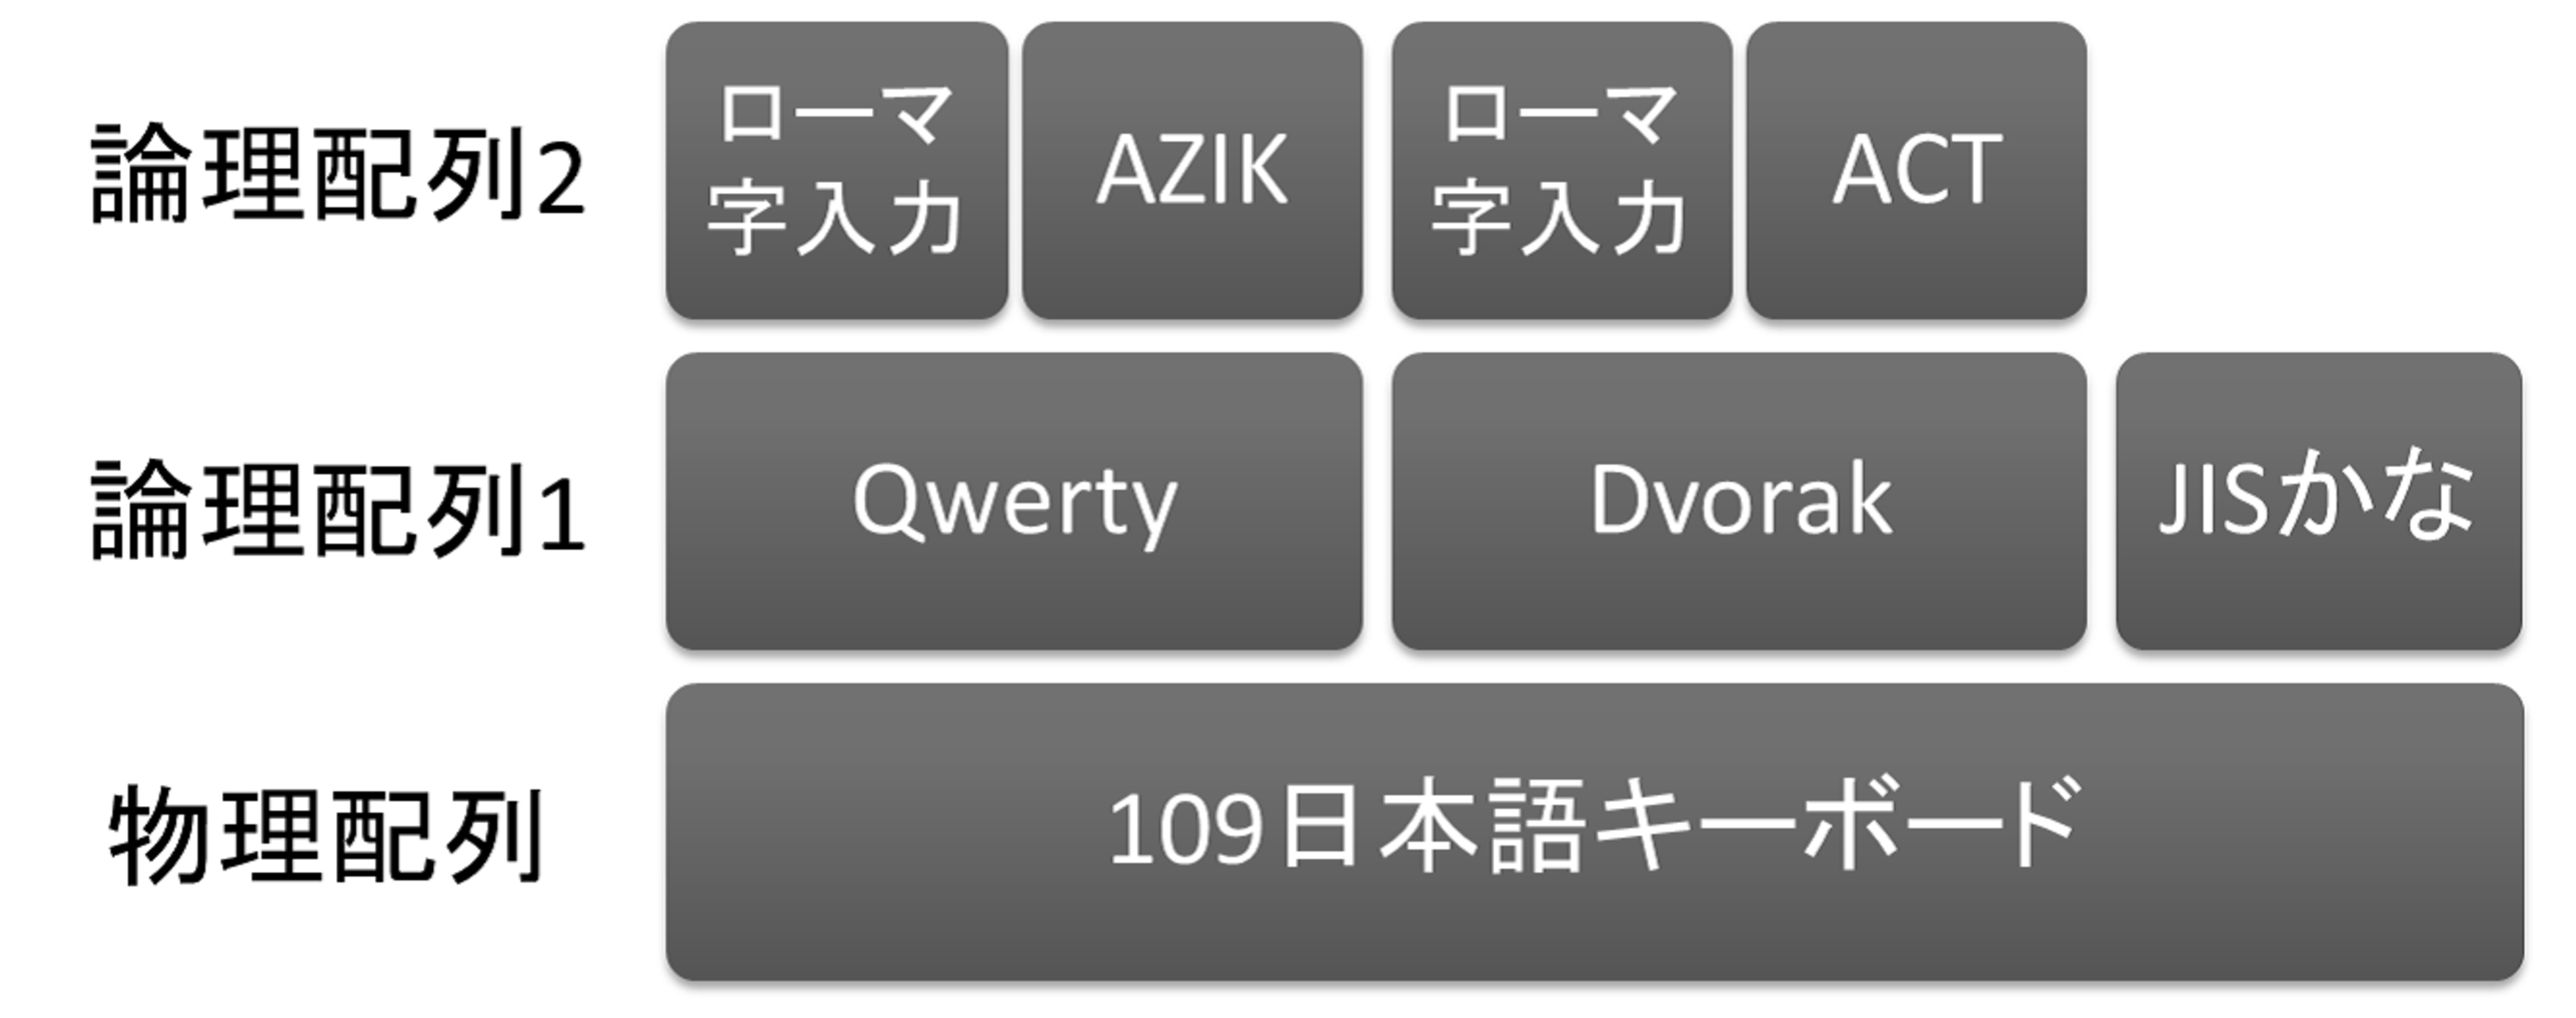
\includegraphics[width=14cm,clip]{res_tomoemon/arrangement.eps}
 \end{center}
 \caption{�����z��Ƙ_���z��̊K�w}
 \label{arrangement}
\end{figure*}

�_���z�����������ƕ�����ƁA�p������͂���z��Ƃ��Ȃ���͂���z��̓��ނɕ����邱�Ƃ��ł��܂�\footnote{�����𒼐ڂł���z�������܂��������ł͊������܂��B}�B���[�}�����͂��ŏI�I�ɂ͂��Ȃ���͂���z��Ȃ̂ŁA�����ł͂��ȓ��͂̈�‚Ƃ��܂��B�������A���[�}�����͉͂p���̑g�ݍ��킹�œ��͂��邽�߁A�}\ref{arrangement}�̂悤�ɉp�����͂̔z��Ɉˑ����Ă��܂��B

\subsection{���͑��x�ƑŌ����x}

����͓��ɓ�����Ƃ͂Ȃ��̂ł����A�u���͑��x�v�u�����v�u�x���v�Ƃ������t���悭�g���̂ŁA���ꂼ��̈Ӗ����m�F���Ă����܂��B�܂��A���͑��x���A[�ۑ�̕�����]��[���͂ɗv��������]�ƒ�`���܂��B���Z�^�C�s���O�ɂ����āA���͂��ׂ������͂��ׂė^�����Ă���̂ŁA������ۑ�̕�����ƌĂсA���̕��������u�ۑ�̕������v�Ƃ��܂��B�����ł͉p���A���ȁA���Ȋ���������Ȃǂ͋C�ɂ��܂���B�܂��A���͉”\�ȏ�ԂɂȂ��Ă�����͂���������܂ł̎��Ԃ��u���͂ɗv�������ԁv�Ƃ��܂��B��̗�Ő�������Ɓu����ɂ��́v��4�b�őł��؂����ꍇ�̓��͑��x��1.25����/�b�ł��B���͑��x���u�����v�Ƃ͂��̓��͑��x�̒l���傫�����ƁA�u�x���v�͂��̋t��\���܂��B
����Ƃ͕ʂɁu�Ō����x�v�Ƃ���������������ꍇ������܂��B����͒P���ŁA�P�ʎ��Ԃ�����ɃL�[�{�[�h�̃L�[������Ō��ł��邩��\�����̂ł��B��ʓI�ɍ����ɑŌ��ł�����������ȓ��͂ɂȂ�܂����A�ϊ�����̓��{����͑��x�������ꍇ�͕ϊ��ɑ�z�����l���Ō����x�ŗ���Ă��Ă����͑��x�ŏ���ꍇ���\���ɂ��肦�܂��B

\section{�Ȃ��z���ς���̂�}

���āA�悤�₭�{��ł����A���������Ȃ��z���ς��Ȃ���΂����Ȃ��̂ł��傤���B�}�C�i�[�z����D��Ŏg�����Ƃ���^�C�p�[������̂͂Ȃ��ł��傤���B��q����ʂ�z���ς���Ƃ����̂͑傫�ȘJ�͂�K�v�Ƃ��܂����A��J���Ĕz���ς��邩��ɂ͂���Ȃ�̃����b�g�����݂���̂ł��B

\begin{itemize}
 \item �w�̓����ɖ������Ȃ��Ȃ�
 \item ���w�Ō�������
 \item �����A�ł�����
 \item �w�̈ړ�����������
 \item �w�̈ړ��͈͂������Ȃ�
 \item �Ō��̉񐔂�����
 \item �������₷���w���d�_�I�Ɏg��
\end{itemize}
�����͂ǂ�������Ō��ɂƂ��ďd�v�ƍl������v�f�ŁA���������݂ɃR���g���[���ł���悤�ɂȂ�̂��u�z���ς���v�Ƃ�����@�ł��B�������z���ς��铮�@�̊̂Ȃ̂ŁA���[�}�����͂��ɏ������������Ă����܂��B

\subsubsection*{�w�̓����ɖ������Ȃ��Ȃ�}
�u�킴�킴�v��łꍇ�A�W���^�w�ł͖�w�Ə��w��\finger{21112111}�ƂȂ�܂����A����͔��ɑł��ɂ����p�^�[���ɂȂ�܂��B�z���ς��邱�Ƃł����������p�^�[�������炵�A�ł��₷���p�^�[���ɕς��邱�Ƃ��ł��܂��B
\subsubsection*{���w�Ō�������}
�u�ʂ��ʂ��v�Ƒłꍇ��\finger{77877787}�ƂȂ��āu�ʁv��ł‚��߂ɐl�����w��2�i�������܂����A���̂悤�Ȏw�̈ړ��͍�������������߁A�ł��邾�����Ȃ��ق����D�܂����ł��B
\subsubsection*{�����A�ł�����}
�u�Ȃ�́v�Ƒłꍇ�unannno�v�ƂȂ�A\key{N}��3��A���őł•K�v������܂����A�����L�[��A���őł‚̂��x���Ȃ�v���ɂȂ�܂��B���̏ꍇ�́unaxnno�v�Ƒł���1�񕪌��炷���Ƃ��ł��܂����A�������u�v������ꍇ�͔����邱�Ƃ��ł��܂���B
\subsubsection*{�w�̈ړ�����������}
�w���ړ����Ȃ��őł‚��Ƃ��ł���Γ��R�����Ȃ�܂�\footnote{�����w�œ����L�[��A�ł���ꍇ�͗�O�I�ɒx���Ȃ邱�Ƃ�����܂��B}�B�z��ɂ���Ă̓z�[���|�W�V��������قƂ�ǎw�𓮂������ɑłĂ邱�Ƃ������b�g�Ƃ��Ă����Ă�����̂�����܂��B
\subsubsection*{�w�̈ړ��͈͂������Ȃ�}
��L�ɋ߂��v�f�ŁA���ȓ��͂̏ꍇ��4�i�g���̂ɑ΂��A���[�}�����͂ł�3�i�����g��Ȃ��Ƃ������z�񂲂Ƃ̈Ⴂ������܂��B�L���͈͂��g������1�Ō��œ��͂ł��镶���̎�ނ������č������ł������A�w�̈ړ��͈͂��L���Ȃ邱�ƂŃ~�X�̏��Ȃ����肵�����͂�����Ȃ�Ƃ����꒷��Z������܂��B
\subsubsection*{�Ō��̉񐔂�����}
��菭�Ȃ��Ō��񐔂œ����������łĂ�悤�ɂ��邱�Ƃ��ł��܂��B���[�}�����͂́u����ɂ��́v��10�Ō��ł����A���ȓ��͂ł�5�Ō��ɂȂ�܂��B
\subsubsection*{�������₷���w���d�_�I�Ɏg��}
�E�����̐l�͓��R�E��̕����������₷���A�܂�������Ɋւ�炸�l�����w�⒆�w���������₷�����ƂƎv���܂��B�z��Ɠ��͂��镶�͂̑g�ݍ��킹�ɂ���Ă͂���ȊO�̎w�𑽂��g���Ƃ��������Ƃ��N���肦�܂��B���̏ꍇ�A���Ȏw����K�ɂ���Ēb����̂�����ł����A�������₷���w���d�_�I�Ɏg���z����g�����ƂŁA�S�̂��猩�Ă�荂���ɑłĂ�悤�ɂȂ�܂��B

�����̓����𓥂܂��A�e�l�ɂƂ��ēK�؂Ȕz��ɐ؂�ւ��邱�ƂŁu���͑��x�������v�Ȃ�܂��B�������A��̒��ł��������Ă���ʂ�A�����͕K�������z���ύX���邱�Ƃł��������Ȃ������b�g�ł͂Ȃ��A�䗬�^�w��������铙�́u�œK���v�e�N�j�b�N�ɂ���ăJ�o�[�ł���͈͂����X����܂��B�������A�Ⴆ�΍œK���ł͑Ō��񐔂����炷���Ƃ͂ł��܂���B�œK�������_��ɁA���Ž��R�ɏ�L�v�f�����P�ł���̂��z���ς���Ƃ�����@�ɂȂ�܂��B�z�񂲂Ƃɓ��ɂǂ̗v�f���d�����Ă��邩�قȂ邽�߁A�z���I������ۂ͎������d���������v�f�Ƃ̃}�b�`���O���d�v�ɂȂ�܂��B

���̏ꍇ��AZIK�Ƃ����z����x�[�X�ɂ������̂��g���Ă��܂��B���̔z��ł̓��[�}�����͂Ŋ��蓖�Ă��Ă��Ȃ��p���̑g�ݍ��킹�ɕʂ̂��Ȃ����蓖�ĂāA���̃��[�}�����͂͂قڈێ����‚A��菭�Ȃ��Ō��̑ł��₷���p�^�[���𑝂₵�Ă��܂��B�Ⴆ�Ε\\ref{tomoemon:compare_roman_azik}�̂悤�ȑł������ł��܂��B

\begin{table}
\begin{center}
\caption{���[�}�����͂�AZIK�̔�r}
\label{tomoemon:compare_roman_azik}
\begin{tabular}{ccc}
\hline
���� & ���[�}������ & AZIK \\
\hline
���� ���� ���� & kan kin kon & kn kk kl \\
���� ���� ���� & sha shu sho & xa xu xo \\
�ɂ� �ɂ� �ɂ� & nya nyu nyo & nga ngu ngo \\
�������� & gakkou & ga;kp \\
\hline
\end{tabular}
\end{center}
\end{table}

���̃��[�}�����͂̑啔�������̂܂܎g����Ƃ�����������A�ʏ�̃��[�}�����͂��g���‚��X�Ɍ����I�ȑł��������Ă������Ƃ��ł���Ƃ��������b�g�������܂����A����䂦�Ɍ��I�ȕω��͖]�߂Ȃ��Ƃ������ƂɂȂ�܂��B���������b�g�Ɗ��������f�����b�g�Ɗ����邩�́A�l���ꂼ��Ȃ̂ŁA�����̖ڎw�����̂Ɣz�񂲂Ƃ̓������悭�m�邱�Ƃ��d�v�ł��B

\section{�z���ύX���ׂ��łȂ�5�‚̗��R}

�����b�g�����������Ă��Ƃ͎��ȐӔC�łƂ����̂��s�e�؂Ȃ̂ŁA�z��ύX���ׂ��łȂ����R�����킹�Đ������Ă����܂��B���ۂ̂Ƃ��냁���b�g�ɂ‚��Ă͂��낢��ȂƂ���ŏЉ��Ă���̂ŁA�d�v�ɂȂ�̂̓f�����b�g�̕��������肵�܂��B�����Ȕz��Ƀ`�������W���ė~��������Ƃ��Ă͌g�ѓd�b�̗����v�����̂��Ƃ�菑���̂悤�ɋɏ��t�H���g�ŏ��������Ƃ���ł����A�f�����b�g������������ł̃`�������W�������߂��܂��B���āA��q�̂悤�ȃ����b�g�����󂷂邽�߂Ɏx�����R�X�g�ƃ��X�N�͏���������܂���B�قȂ�z����K�����邽�߂ɂ��Ȃ��͏��Ȃ��Ƃ����̓�‚��o�傷��K�v������܂��B
\begin{itemize}
 \item ���Ƃ��Ǝg���Ă����z��ɂ�������K���Ԃ̌���
 \item ���Ƃ��Ǝg���Ă����z��Ƃ̍����̉”\��
\end{itemize}
�܂��A�قȂ�z��K���Ɏ��g�ޏ�Ŏ��̂悤�ȍ���ɑ�������”\��������܂��B
\begin{itemize}
 \item ���K���@���m�����Ă��Ȃ�
 \item �����L���O�ւ̎Q��Ȃǂ��F�߂��Ȃ�
 \item ��p�̃\�t�g�𓱓����Ȃ���΂Ȃ�Ȃ�(Linux���Ŏg���Ȃ��”\��)
\end{itemize}
�܂��A���Ƃ̔z��ւ̉e���ł����A����܂Ń��[�}�����͂ŗ��K���Ă����l���u���ꂩ��͂��ȓ��͈�r�ł���Ă������v�ƌ��f�����Ƃ���ƁA���̏u�Ԃ����Ƀ��[�}�����͂̓��͑��x�͐����Ă����΂���ł��B�������A�����ɑłĂȂ��Ȃ邱�Ƃ͂���܂��񂵁A�����̓��͑��x���ێ��ł���ꍇ������܂��B�������A�z���؂�ւ������ƂŌ��̔z��̓��͑��x�����シ�邱�Ƃ͊�{�I�ɂ���܂���B��{�I�ɂƌ������̂́A���Ƃ��ƃ^�C�s���O���S�҂������ꍇ�Ȃǂ́A�ʂ̔z��ɐ؂�ւ��Ă�����K���d�ˁA������̔F�����x��w�̉^���\�͂����コ���邱�ƂŁA���̔z��ɖ߂����^�C�~���O�ňȑO��葬���łĂ�悤�ɂȂ��Ă��邱�Ƃ͏\�����肦�܂��B�������A���łɌ��E�Ɗ����鑬�x�܂ŗ��K���Ă���z���ύX�����ꍇ�ɁA�z���߂��đ����Ȃ邱�Ƃ͂܂�����܂���B

�͂��߂ɂ������܂������A�z���؂�ւ��邱�Ƃ͌��̔z��ɂ����鐬���̉”\�����̂ċ��邱�ƂƓ��`�ł��B���Ȃ������K�ɔ�₹�鎞�Ԃ�100�Ƃ��āA100�̎��Ԃ��ׂĂ����[�}�����͂Ɏg���Ă���Γ��B�ł�����������Ȃ��������̂ĂāA�ʂ̔z��ɓq����̂ł��B����́A�V�����z��̗��K���Ԃ�50�����Ƃ��āA�c��50�̓��[�}�����͂ɔ�₷�悤�ȏꍇ�����l�ł��B���[�}�����̗͂��K���Ԃ������ɂȂ邱�ƂŊm���Ƀ��[�}�����͂̐����͒x���Ȃ�܂��B

����ɉ����āA���Ƃ��Ƃ���Ă����z�񂪂���ɒx���Ȃ�v���Ƃ��ĐV�����z��Ƃ̍������������܂��B�����Ɋւ���m���͂��܂��ɏ\���W�܂��Ă���Ƃ͌����������󋵂ł����A�p���z�񓯎m(Qwerty��Dvorak��)�₩�Ȕz�񓯎m(JIS���Ȃƌ��z��)�A���[�}�����͌n���m(Qwerty��AZIK��)�ł͍�������������”\���������ł��B��������������ƗႦ�΁u����ɂ��́v��Qwerty���[�}�����͂őł��Ȃ��Ƃ����Ȃ���ʂŁAAZIK���Ɂuklnitiha�v�Ƒł��Ă��܂����Ƃ�����܂��B�ȑO��������Ƃ̂���z��Ɠ��n���̔z���V���ɏK�����悤�Ƃ���ꍇ�́A�ȑO�̔z�񂪎g���Ȃ��Ȃ邱�Ƃ��o�債�Ă����������ǂ��ł��傤�B

���ꂾ���ŏ\���n�[�h���������̂ł����A����ɗ���������Ȃ���΂Ȃ�Ȃ���������܂��B
���K���@���m�����Ă��Ȃ��z��̗��K������ۂ͎����Ō����I�ȗ��K���@���l����K�v������܂��B�Ⴆ�Ύ��̏ꍇ�AAZIK����K����ۂ́A�V���Ɋ��蓖�Ă�ꂽ���[�}���̑g�ݍ��킹�������Ȃ肷�ׂē������ė��K����͓̂�����߁A��‚����ԂɎ����ꂽ�P�����K���Ă����悤�ɂ܂����B�܂��A�򒹔z��ł̓V�t�g�L�[���g���ꍇ�Ƃ����łȂ��ꍇ�𕪂��ė��K���s���܂����B����܂łɎ��g�񂾔z��Ɨ��K���@�ɂ‚��Ă͌�q���܂��B

����ɁA���Ȃ����I�񂾔z��̓^�C�s���O�\�t�g�̃����L���O����ւ̎Q�킪�F�߂��Ȃ��”\��������܂��B�Ⴆ�΁A�^�C�v�E�F���ɂ�����AZIK�͎Q�l�L�^�����ƂȂ��āA�ʏ�̃����L���O�Ɠ��������ɂ͂Ȃ�Ȃ����Ƃ���������Ă��܂��B�܂��A�����p�\�R�����̓R���N�[���̏ꍇ�́A�e�Q���҂̎���ő�����s���\�I�ł͊e��z�񂪑I���”\�ł����A������ł͊�{�I�ɂ̓��[�}�����͂����ȓ��͂����I���ł��܂���B���p�\�̂悤�Ȍ��I�ȑ��ɂ����Č���F�߂��Ă��Ȃ��z��ł̎Q����F�߂����邱�Ƃ͑傫�ȍ���𔺂��ł��傤�B

���p�\�̂悤�ȑ��œ���z�񂪎g���Ȃ������̈�‚ɂ��Ȃ��Ă���̂��A�z��ɂ���Ă͐�p�̃\�t�g�E�F�A�𓱓����Ȃ���Ύg�����Ƃ��ł��Ȃ��Ƃ����_�ł��B��p�̃\�t�g�Ƃ����Ă���{�I�Ƀt���[�\�t�g�œ����������܂œ���Ȃ����߁A�����������Ă��܂��Ί�{�I�ɖ��͂Ȃ��̂ł����A��p�\�t�g���K�v�ɂȂ邱�ƂŎ��̂悤�Ȗ�肪�N���肦�܂��B
\begin{itemize}
 \item OS�̃o�[�W�����A�b�v�ɂ�肱��܂Ŏg���Ă����\�t�g���g���Ȃ��Ȃ���
 \item �قȂ�OS�������Ă���PC�Ŏg���Ȃ�����
 \item ��Ђ�PC�ȂǑ��̊‹��œ����z����g���������\�t�g�𓱓��ł��Ȃ�
\end{itemize}
�ň��̏ꍇ�A�u����ł͐e�w�V�t�g���g���Ă��邯�lj�Ђł̓��[�}�����͂��g��Ȃ��Ă͂Ȃ�Ȃ��v�Ƃ������ꍇ�͏\���ɂ��肦�܂��B���������Ӗ��ł��z�񓯎m�̍����̉”\���ɂ͏\�����ӂ���K�v������A�܂��A�������g���”\���̂���PC�ɐ�p�\�t�g�������邩�͎��O�Ɍ������Ă����ׂ��ł��B


\section*{�z��ύX�̋�̗�}

���̏͂���͎����g�̔z��ύX�̌o���ɂ‚��ďЉ���Ă��������܂��B�����܂łł��łɏ����Ă��镔��������܂����A�z���ύX����ɂ������Č����������ƁA���ۂɕς��Ă݂Ċ��������ƁA���������邽�߂ɍH�v�������ƂȂǂ�U��Ԃ�A�݂Ȃ���̔z��ύX�̎Q�l�ɂ��Ă���������΂Ǝv���܂��B

�\\ref{tomoemon:history}�͎�������܂łɌo�������z��N�\�ɂȂ�܂��B���B���x�̓^�C�v�E�F������R�A����K�ɂ������{��p�ꃂ�[�h�̃����N�ŕ\���Ă��܂��B
\begin{table}
\begin{center}
\caption{�M�҂�����܂łɌo�������z��}
\label{tomoemon:history}
\begin{tabular}{ccc}
\hline
�z�� & ���K���� & ���B���x \\
\hline
Qwerty���[�}�� & 1997�`2009 & ZI \\
JIS���� & 2001�`2003 & XA \\
Dvorak���[�}�� & 2004 & D \\
�Ў�`���C����(�E��) & 2005 & SF \\
�򒹔z��290 & 2005�`2008 & XS \\
AZIK & 2008-2009 & XX \\
tomoemon-AZIK\footnotemark & 2009�` & ZH \\
\hline
\end{tabular}
\end{center}
\end{table}
\footnotetext{�M�҂ɂ��AZIK�̓Ǝ�����}
���̒��œ��ɐe�w�V�t�g�n�ł���򒹔z��ƃ��[�}�����͌n�ł���AZIK�̌o���ɂ‚��ďЉ���Ă��������܂��B

\section{�z��ύX�̗�1 - �򒹔z��}

\subsection{����}

�e�w�V�t�g�n�̔z��ł��B�}\ref{asuka}\footnote{�}�� \url{http://ameblo.jp/asuka-layout/entry-10334710008.html} ���}�̂悤��1�‚̃L�[�ɕ����̂��Ȃ����蓖�Ă��Ă��āA����L�[�������ۂɐe�w�V�t�g�𓯎��ɉ����������Ȃ����œ��͂��邩�Ȃ�؂�ւ��܂��B�u�e�w�V�t�g�Ȃ��ʼn����v�A�u���e�w�V�t�g�������Ȃ��牟���v�A�u�E�e�w�V�t�g�������Ȃ��牟���v���Ƃ�1�‚̃L�[��3��ނ̂��Ȃ���͂��邱�Ƃ��ł��܂��B�e�w�V�t�g�̑�\�i�ł���NICOLA�Ƃ̑傫�ȈႢ�͐e�w�V�t�g�̃��[���I�[�o�[�ł��B�򒹔z��ł́A�e�w�V�t�g�L�[���������ςȂ��ŃL�[�𕡐������Ă����ƁA���ׂẴL�[�Őe�w�V�t�g���K�p���ꂽ���Ȃ��o�͂���܂��BNICOLA�ł͂��Ƃ������e�w�V�t�g�L�[���g��2��������͂���ꍇ�ł��A1�����ڂʼn������e�w�V�t�g���������񗣂��Ă��������x�����K�v������܂��B


\begin{figure*}
 \begin{center}
   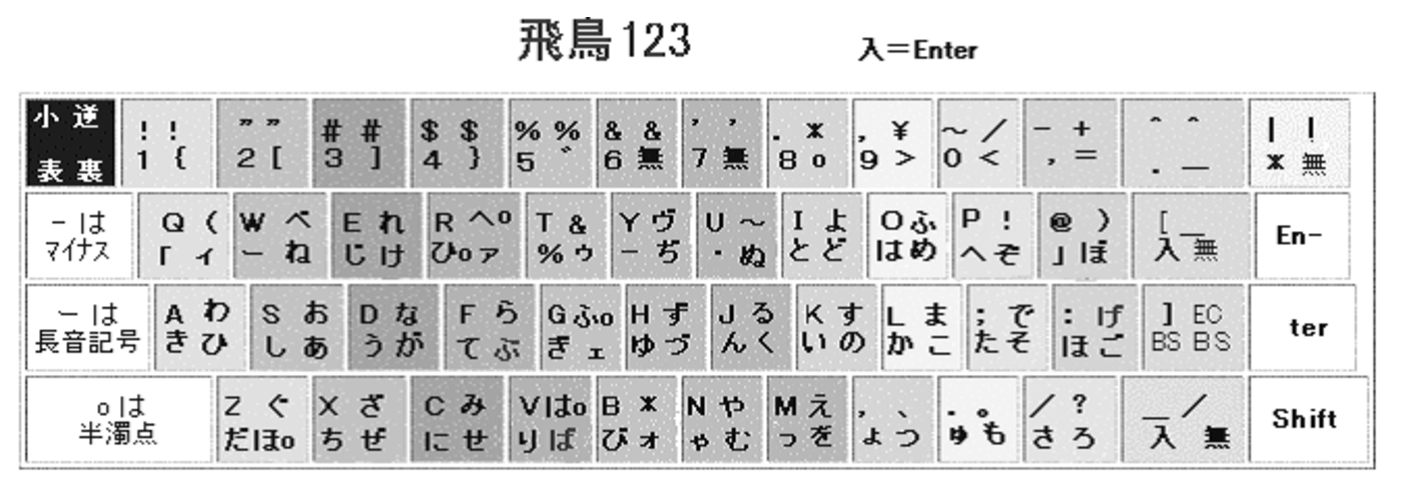
\includegraphics[width=14cm,clip]{res_tomoemon/asuka.eps}
 \end{center}
 \caption{�򒹔z��123-383��}
 \label{asuka}
\end{figure*}

\subsection{���@}

���̎����ɔ򒹔z����n�߂����R���ӏ������ɂ���ƈȉ��̂悤�ȓ��e�ɂȂ�܂��B
\begin{itemize}
 \item Qwerty���[�}�����͂̐����Ɍ��E�������Ă���
 \item ���{����͂ɂ����Ă̓��[�}�����͂ɔ�ׂĂ��ȓ��͂̕��������͖̂��炩
 \item JIS���Ȃ͉ߋ��Ɏ��g�񂾌���4�i�g�������������ɍ���Ȃ�
 \item ���܂��ܔ򒹔z����Љ�Ă������
\end{itemize}
1�–ڂ͂ǂ��炩�Ƃ����Ə��ɓI�ȗ��R�ŁA�܂��ɖ{�L���́u�͂��߂Ɂv�ŏq�ׂ��󋵂ɂ����āA���ɂ�������悤�ȋC�����ő��̔z�������Ă݂悤�Ǝv���܂����B���U��Ԃ��Ă��AQwerty���[�}���ł����Ɨ��K����΃^�C�v�E�F���ɂ�����ō������N�͂��������グ�邱�Ƃ͂ł���Ǝv���܂����A�����̎��_��Qwerty���[�}�����͂̑ł��ɂ����������ڂɂ‚��Ă������߁A�����ɂ��̗��K������C���N�����A�����ς�Ƃ�����̉”\���͐؂�̂Ă܂����B

2�–ڈȍ~�̗��R�ɂ‚��āA���ȓ��͂ƈꊇ��Ɍ����Ă�JIS���Ȃ�򒹔z��ȊO�ɂ������̔z�񂪑��݂��Ă���A�������򒹔z���m��O�Ɍ��z����Љ��Ă����̂ł����A���Ƃ��Ɛe�w�V�t�g�ɋ����������Ă������Ƃ���򒹔z��Ɍ��߂܂����B�̂̃��[�v�����̓R���e�X�g�ł͐e�w�V�t�g���̗͂��p�҂����𑍂Ȃ߂ɂ��Ă����A�Ƃ����悤�Șb���悭�����Ă������Ƃ���A���R�Ɛe�w�V�t�g�͂������Ƃ�����ۂ�����܂����B����ŁA�e�w�V�t�g�ɂ‚��Ē��ׂĂ݂�ƁA�V�t�g���s�������Ō������珜���Ă����������ɏ��Ȃ��Ō����ŏЉ��悤�ȗႪ���X����A�኱�����񂭂����ȂƂ�����ۂ������Ă��܂����B
��X�ɂȂ��Ē��ׂĂ݂��Ƃ���ł́A�O�҂ɂ‚��Ă͕p�o�P��������o�^�̂悤�Ȍ`�œo�^���Ă��������̂悤�ł���A���ǃ^�C�p�[�����߂�悤�ȓ��͑��x��e�ՂɎ����ł�����̂ł͂Ȃ����Ƃ��킩���Ă��܂��B

���̂悤�ɁA�e�w�V�t�g���g�����Ƃň��|�I�ȑ��x��������킯�ł͂Ȃ��Ƃ����F�������߂��炠�����̂ł����A�����̒m�����^�C�p�[���e�w�V�t�g�Ō��E�t�߂܂ŗ��K������𕷂������Ƃ��Ȃ������̂ŁA�`�������W���[�Ƃ��Ă���Ă݂����Ƃ����C�����������ɂ������z��I���������Ǝv���܂��B

\subsection{���K���@}

�ߋ��̔z��K�����̗��K�͂��ׂāu�����Ȃ�^�C�v�E�F�����N�����đł��n�߂�v�Ƃ����ɂ߂ĒP���ȗ��K���@�������̂ł����A�򒹔z��ł�1�‚̃L�[��3�‚̂��Ȃ����蓖�Ă��Ă���A���̗��K���@�ł͂Ȃ��Ȃ��L�[�̈ʒu���o�����Ȃ��Ǝv���A�ꕔ�̃L�[��e�w�V�t�g�������g�����P������Ԃɗ��K���Ă����Ƃ������@�����܂����B

���̍ہA�u�򒹂̂��߂Ɂv�Ƃ����P��W�������Ă��������A�ȉ��̂悤�ȃp�^�[���ŗ��K���s���܂����B����5,6,7�Ɛi�ނɂ‚�ĕp�x�̒Ⴂ�������܂񂾒P��ɂȂ��Ă����܂��B
\begin{itemize}
 \item ����1: �V�t�g�����z�[���|�W�V����
 \item ����2: �u�ł��v�u�܂��v�u����v���̕����ƘA���V�t�g�̌�
 \item ����3: �V�t�g����z�[���|�W�V����
 \item ����4: �E��̏㉺�i�i�����Ƒ�����\ruby{�X��}{�悤����}���܂ށj���K������
 \item ����5-7: 1�`4�ȊO�̂���
 \item ����8: 1���[�h���ɃV�t�g�̐؂�ւ����������
\end{itemize}
���̗��K���@�͏��߂��炷�ׂĂ̂��Ȃ���������ɍ������P��̗��K������������Ȃ�������ǂ��A���̌��AZIK�̗��K�̍ۂɂ�������Ă��܂��B
�Ƃ����̂��A���߂ė��K����z��ł�1�������͂��邽�тɖ��񂩂Ȃ�z��}�̒�����T�����ƂɂȂ�܂��B�T���Ă͑ł��A�T���Ă͑ł������x���J��Ԃ��ď������“��Ƒ̂Ɋo�����܂��Ă����̂ł����A���ׂĂ̂��Ȃ��܂񂾒P�����K���Ă���Ɣz��}�̒����炩�Ȃ̈ʒu��T�����Ԃ����ɒ����Ȃ�܂��B�A���t�@�x�b�g�ł����26�‚���T���΂悢�����ł����A�򒹔z��̏ꍇ��70�ȏ�̂��Ȃ���T���Ȃ���΂Ȃ�܂���B
�v���O���~���O�̐��E�ł����������Ƃ����ĕ��G�Ȗ��𕪉����Ă����āA�ł��邾���P���ȕ��@�ʼn������‚���Ƃ����l����������܂����A�z����K������ۂ��ł��邾�����K�Ώۂ̔z��𕪊����ĒP���ŊȒP�ȗ��K�ɂȂ邱�Ƃ�S������̂��ǂ��ł��傤�B


\subsection{���K����}

�ŏI�I��2008�N�̒i�K�Ń^�C�v�E�F������K�Ŋ�{��p��XS�A����XA�ɓ��B���܂����B�ŏI�I�ɂƏ������̂͑��x�ʂł͂��ꂪ�قڌ��E�ŁA����ȏ�̑��x�����肵�ďo�����Ƃ͓���Ɣ��f��������ł��B2011�N���݂Ń^�C�v�E�F������K�̊�{��p��1�ʂ̃����N��ZD�ł��邱�Ƃ��l����ƁA�����ɂ��y�΂Ȃ������Ƃ����̂��q�ϓI�Ȏ����ł��B�X�l�̔\�͂̍������邽�߁A���ȊO�̃^�C�p�[�����g�߂΂����Ə�ɍs����”\���͂���܂����A��͂�e�w�V�t�g���g���Ƃ������������Ɗ����܂����B

JIS���ȓ��͂⃍�[�}�����͂Ƒ傫���Ⴄ�̂́A��͂�e�w���g���ăV�t�g�L�[�𑼂̂��ȃL�[�Ɠ����ɉ�������ł��B�z��ύX�\�t�g�̐ݒ�ɂ���ẮA�e�w�V�t�g�������Ă��炩�Ȃ������ꍇ�����ł͂Ȃ��A�t�ɂ��Ȃ������Ă���e�w�V�t�g���������ƂŃV�t�g���K�v�ȕ�������͂ł��܂��B����̓V�t�g�������^�C�~���O�ɋ��e�ł���덷���܂߂Ă����Ƃ������ƂȂ̂ł����A���̌o���ł͍����ɑłĂ�悤�ɂȂ��Ă���Ƃ��̋��e�덷�ɂ��~�X�������������߁A�u�e�w�V�t�g�������Ă��炩�Ȃ������ꍇ�ɂ̂݃V�t�g��L���ɂ���v�ݒ�ŗ��K���Ă��܂����B�������A����ł����͑��x�������Ȃ�΂Ȃ�قǐe�w�V�t�g�������^�C�~���O���V�r�A�ɂȂ��Ă��邽�߁A�V�t�g�̂���ɂ��~�X�̔����������ɂȂ�܂��B����͔򒹔z��Ɍ��炸�e�w�V�t�g�n�S�ʂɌ�����̂ł͂Ȃ����Ɗ����܂����B

��L�̒ʂ�A�򒹔z��̎��g�݂͑��x����Ƃ����ϓ_���猾���Ύ��s�ł��B
�������͂������̐e�w�V�t�g�̓����ɂ‚��Ă�����x�c���ł����A�z��K���̌����ǂ����K���@�ɂ‚��Ċw�Ԃ��Ƃ��ł����Ƃ��������b�g�͂���܂������A����ŗǂ������Ɣz��K�����J��Ԃ��Ă����͂����̔z��}�j�A�ɂȂ��Ă��܂��܂��B�{�C��(���Ȃ��Ƃ��Z���Ԃ�)�g�b�v�^�C�p�[��ڎw���l�ɂƂ��Ă͂��̂悤�Ȏ��g�݂͔����������ǂ��ƒf�����܂��B�����ɍł��K������‚̔z��ɂ��ׂĂ̗��K���Ԃ𒍂����ނ��Ƃ������A���͑��x��b�����Ԃ̕��@������ł��B


\section{�z��ύX�̗�2 - tomoemon-AZIK}

\subsection{����}

AZIK�͂��łɏЉ���Ƃ���AQwerty���[�}�����͂��x�[�X�ɂ��ďȑŌ����̓��[����lj������z��ł��Btomoemon-AZIK��AZIK�̃��[�����قڂ��̂܂܎g���‚A����ɓƎ��̏ȑŌ����[����lj������z��ɂȂ�܂��B���ɁA�\\ref{tomoemon:compare_roman_azik_tomoemon_azik}�̂悤�Ɂu���v�u�ށv�Ƃ��������Ȃ���͂���ۂɔ������铯�w�Ō����ł��邾��������p�^�[����lj����Ă���̂������ł��B
\begin{table*}
\begin{center}
\caption{���[�}�����́AAZIK��tomoemon-AZIK�̔�r}
\label{tomoemon:compare_roman_azik_tomoemon_azik}
\begin{tabular}{cccc}
\hline
���� & ���[�}������ & AZIK & tomoemon-AZIK \\
\hline
�ނ� �ނ� �ނ� & muta muti mutu & mfta mfti mftu & mta mti mtu \\
���� ���� ���� & kita kiti kitu & kfta kfti kftu & kta kti ktu \\
\hline
\end{tabular}
\end{center}
\end{table*}


\subsection{���@}

�򒹔z��̎��Ɏ��g�񂾔z��AZIK�ŁA�����I�ɂ͔򒹔z��ő���XA���o�������N��Ɏn�߂Ă��܂��B�ڂ������@�ɂ‚��Ă͎��̓����̓��L�����Ԃ��Ă������Ă��Ȃ��̂Ŋm���Ȃ��Ƃ͏����Ȃ��̂ł����A�����炭�򒹔z��̗��K�o�����琶�܂ꂽ���̓�_���傫�ȗ��R�������Ǝv���܂��B�򒹔z��̏K���܂łɎ��Ԃ����������̂ŁA�w�K�R�X�g���Ⴛ���Ȃ��̂ɐH�w���������̂���_�B������_�͔򒹔z��͐e�w�V�t�g�Ƃ����V���ȓ����ɂ���đ��x�̐������������Ă��܂������A�����̔z������P���č�����z��Ȃ�Ώ]�����������Ȃ�̂͂قڊm���ł��낤�Ƃ������ƁB
���̂悤�ɍl����ƁA���Ƃ���AZIK�Ɋ֐S�������Ă������Ƃ�����A�򒹔z��̂��Ƃ�AZIK��I�񂾂͕̂K�R�������̂�������܂���B

\subsection{���K���@}

\subsubsection*{�p�^�[���������K}
�򒹔z��̗��K���Ɠ��l�ɁAAZIK�ł��V���ɒlj����ꂽ�ȉ��̃p�^�[�������Ԃɗ��K���Ă������@�����܂����B

\begin{itemize}
 \item �w���x��p�L�[
 \item �w�V���x�w�`���x�s�L�[�A�����L�[
 \item �w����x\ruby{����}{�͂‚���}�g��
 \item �w�@���x�w�D���x�w�F���x�w�H���x
 \item �w�[�x�����݊��L�[
 \item �u�x�v�̑���́u�f�v
 \item �u�y�v�̑���́u�m�v
 \item �u�t�v�u�h�v���̑���́u�e�v
 \item �O����̓��́i�O������͊g���j
\end{itemize}

���ꂼ��ȉ��̂悤�ȒP�����K���Ă��܂��B
\subsubsection*{�p�^�[��1�F�w���x��p�L�[}
�u���v��\key{;}�̃L�[�P�Ƃœ��͂��邱�Ƃœ��w�Ō������炵�܂��B
\begin{itemize}
 \item �o�b�O [ba;gu]
 \item �J���b�g [kara;to]
\end{itemize}

\subsubsection*{�p�^�[��2�F�w�V���x�w�`���x�s�L�[�A�����L�[}
�u����v�s�́ux�v�A�u�`���v�s�́uc�v���q���Ƃ��Ďg���A�usha�v�ucha�v�ȂǂƔ�ׂĈ�Ō����炷���Ƃ��ł��܂��B
\begin{itemize}
 \item ���傤���� [xousei]
 \item �������� [ataxa]
\end{itemize}

\subsubsection*{�p�^�[��3�F�w����x�����g��}
���Ɂu��v�����������͖{���̕ꉹ�L�[��1�‰����g���܂��B�u����v�̏ꍇ��\key{O}��1�‰���\key{L}���g����\key{M}\key{L}�Ƒł‚��Ƃň�Ō����炷���Ƃ��ł��܂��B
\begin{itemize}
 \item ���񂾂� [mldai]
 \item �݂�� [mkna]
\end{itemize}

\subsubsection*{�p�^�[��4�F�w�@���x�w�D���x�w�F���x�w�H���x}
�����p�x�ŏo������ꉹ�̘A�����ЂƂ܂Ƃ߂ɂ����p�^�[���ł��B�u�q���{ai�v���u�q���{q�v�A�u�q���{uu�v���u�q���{h�v�A�u�q���{ou�v���u�q���{p�v�Ƃ��������[�}���Ɋ��蓖�Ă邱�Ƃ�1�Ō����炵�܂��B
\begin{itemize}
 \item �����Ƃ� [gptp]
 \item �悤���� [ypkq]
\end{itemize}

��L�̂悤�ȃ��[�}���̃p�^�[���ɑ΂��āA���ꂼ�ꃏ�[�h�𐔕S�‚��’��o����WeatherTyping�ŗ��K����Ƃ������@�����܂����B�e�p�^�[���ɂ‚��Ă̗��K�e�L�X�g���蓮�ō���Ă����̂��ʓ|�������̂ŁA�u�z��K����tomo�v�Ƃ����e�L�X�g���o�t�B���^�\�t�g���쐬�����̂ŁA�����̂�����̓O�O���Ă݂Ă��������B�\�t�g���̂Ŏ����t�@�C���������Ă��āA�w�肵���p�^�[���̃��[�h�������I�ɒ��o���邱�Ƃ��ł��܂��B

\subsubsection*{�p�^�[���œK�����K}
AZIK���K�œ���|�C���g�̈�‚��P���ɐV�����lj����ꂽ���[�����ق��ق��g���Ă���Ηǂ��킯�ł͂Ȃ��Ƃ����_�ł��B�ǂ��������Ƃ��Ƃ����ƁA�V�����lj����ꂽ���[�����g���ƁA�t�ɑł��Â炭�Ȃ��Ă��܂��ꍇ������Ƃ������Ƃł��B�Ⴆ�΁u�M�K�o�C�g�v�Ƃ����������ł‚Ƃ��͎��̂悤�ɂȂ�܂��B

\begin{itemize}
 \item AZIK: �M�K�o�C�g [gigabqto]
 \item Qwerty: �M�K�o�C�g [gigabaito]
\end{itemize}

�茳�ŏ��������Ă݂ė~�����̂ł����A\key{B}����\key{Q}�ɏ��w��L�΂��̂����‚��AQwerty���[�}�����͂̒ʂ�ɑł����ق����y�ɂȂ邱�Ƃ��킩��܂��B�������A�l�ɂ���Ă�AZIK�̃p�^�[���̕����ł��₷���Ƃ����������邩������܂��񂪁A����܂Ŏg��Ȃ��L�[�����[�}�����͂Ŏg�����Ƃɂ���āA�t�Ɏw�̓��������‚��Ȃ��Ă��܂��p�^�[���Ƃ����̂����݂��܂��B
�ǂ̃p�^�[�����ǂ̏ꍇ�Ɏg���āA�ǂ̏ꍇ�Ɏg��Ȃ��̂������ɂ߂�̂�AZIK�̗��K�ł͔��ɏd�v�ɂȂ�܂��B

���̏ꍇ�͊e��^�C�s���O�\�t�g�ŗ��K���Ă�������AZIK�̃p�^�[���ʂ�ɑł‚Ƒł��ɂ����Ȃ�p�^�[����\\ref{tomoemon:later_azik}�A�\\ref{tomoemon:non_azik}�̂悤�ɂ܂Ƃ߂Ă����܂����B����Ɋւ��Ă͐l�ɂ���đ傫�������o��̂ŁA�݂�Ȃ��݂�Ȃ��̂Ƃ���ɂȂ�킯�ł͂���܂���B���ہA�u���O�ɑł��ɂ����p�^�[������������u�����v�́uss�v�̕��������Ƃ����������܂����B�����AAZIK�̗��K������ۂ͂��̂悤�Ȏ��������ȃp�^�[���͋C�Â�����܂Ƃ߂Ă����A�ł��邾���g��Ȃ��悤�ɂ��邩�A���邢�͔O����ɗ��K���邱�Ƃ�S������̂��ǂ��ł��傤�B

\begin{table*}
\begin{center}
\label{tomoemon:later_azik}
\caption{AZIK�g�����g�����Ƃ�Qwerty�����x���Ȃ�p�^�[��}
\begin{tabular}{cccl}
\hline
���� & AZIK & ���[�}������ & �⑫ \\
\hline
���� & ss & sei & \\
�f�B�X�N & dcisuku & dhisuku & ��X [dyi] �Łu�ł��v��łĂ�悤�ɕύX \\
�e�B�[ & tgi- & thi- & ��X [tyi] �Łu�Ă��v��łĂ�悤�ɕύX \\
�X�|���W & suplji & suponji & �������K�������猋�\�ł��₷���Ȃ��� \\
�A���P�[�g & annke-to & anke-to & ��X�u@�v�ł��u��v����͂ł���悤�ɕύX \\
XaXai: �킩���� & wakq & wakai &  \\
�ۂ��� & po;to & potto & �E�菬�w����� \\
\hline
\end{tabular}
\end{center}
\end{table*}

\begin{table*}
\begin{center}
\label{tomoemon:non_azik}
\caption{���ɑI����������A��{�I�ɂǂ̏�ʂł��g��Ȃ���������AZIK�g��}
\begin{tabular}{ccl}
\hline
���� & AZIK & �⑫ \\
\hline
���� & ss & ���w�Ō��ɂȂ�̂�sei�̕����ǂ� \\
x��: ��� & wz & wn�̕����ł��₷�� \\
�΂� & bq & ���ʂ�bai�̕����y \\
\hline
\end{tabular}
\end{center}
\end{table*}

���̓_���番����ʂ�AAZIK�͈�‚̕�����̑ł‚ɂ��Ă�Qwerty���[�}�����͂ɔ�ׂđ����̑ł��������݂��܂��B���߂̂����͂ǂ̃p�^�[�����ǂ̏�ʂŎg�����𓪂ň�ˆ�Šm�F���ė��K����K�v������A�����ȃ^�C�s���O��ڎw���Ȃ�΂����̂Ɋo�����܂��Ȃ���΂Ȃ�܂���B

\subsection{���K����}

Qwerty���[�}�����͂����P�����z��Ȃ̂�����A�K�������Ȃ邾�낤�ƊÂ����ʂ��������̂ł����A���ۂɃ^�C�v�E�F���̋L�^�����S�ɓh��ւ���ꂽ�̂�1�N�ȏ�o�������Ƃł����B�Ƃ����Ă��A�����݂�����Ɨ��K���Ă����킯�ł͂Ȃ��^�C�v�E�F�����v���C���������ł����Ɩ�90���ɂȂ�܂��B

���Ԃ����������̂͂�͂���K���@�̍��ɏ������A�ǂ̃p�^�[�����ǂ��Ŏg������̂Ɋo�����܂���_�ł��B�܂��AAZIK����tomoemon-AZIK�ւ̑啝�ȃp�^�[���lj��̌����Ƃ������A�{���̔z����K���班�����ꂽ�ӏ��ł����Ԃ�v���܂����B�z��̉����́A��x�n�߂�Ǝ������[������`�ɂȂ�܂łɎ��Ԃ������邱�Ƃ������āA�K�����������^�C�s���O��ڎw���l�ɂ������߂���킯�ł͂���܂��񂪁A���̏ꍇ�͌��ʓI�ɔ��ɖ����̂����z��ɂł����Ǝv���Ă��܂��B
�����ł��������Ƃ͓��R���Ɂu��葬���ł‚��Ƃ��ł���v���Ƃł���A����Ɂu�ł��₷���Ȃ����v�Ƃ������Ƃł�����܂��B����܂łɏK�������z��͂��ׂă^�C�s���O�\�t�g�őł‚��߂̔z��ł����Ȃ������̂ł����Atomoemon-AZIK�����ɑł��₷�����Ƃ�����A���݂͎d����u���O�������Ƃ�����PC���g�����ׂĂ̏�ʂł��̔z����g�p���Ă��܂��B
���Z�^�C�s���O�ɂ����鍂������ڎw����ŕK���������p�ʂ̑ł��₷�����d������K�v�͂���܂���B�Ȃ��Ȃ�A���Z�^�C�s���O�͊�{�I�ɃR�s�[�Ō��ŁA���p�ʂł͊�{�I�ɑn��Ō��Ƃ����傫���قȂ�X�^�C��������ł��B�����g�����Ƃ��Ɠ���ɂ�����g�p�܂ōl���Ă����킯�ł͂Ȃ��̂ŁA���̌��ʂ͋��R�̎Y���ƌ����Ă����ł��傤�B�����AAZIK�𓱓�����̏�Ő�p�\�t�g���K�v�Ȃ��Ƃ����_���ePC�ɓ������₷���Ƃ��������b�g�𐶂�ł���̂͊m���ł��B


\section{�ǂ�����Ĕz���I�����ׂ���}

�����܂Ŕz��K���̎��s����ɂ‚��ďЉ�Ă��܂����B���ꂩ��V���ɔz����K�����悤�ƍl���Ă���l�́u�ߋ���A�z�������Ă����l�͔z��X�AB�z�������Ă����l�͔z��Y�v�̂悤�ȁu�z��I���t���[�`���[�g�v�����҂���Ă�����������܂���B�������ɂ����������̂�����Ε֗��ł����A����܂Ő������Ă����ʂ�ǂ̔z������ɕ��G�ȓ����������Ă��܂��B�V���ɏK������l�ɂ���Ă���ɐV�������������‚���”\��������܂��B����ɁA�K�����悤�Ƃ���l�̓��ӂȎw�̓����Ƃ������悤�ɐl���ꂼ��̓���������܂��B�����_�ł��̗��҂�g�ݍ��킹���t���[�`���[�g�����͓̂���̂ŁA�����̎��������ǂ�ł��邠�Ȃ��ɂ��C���������Ǝv���܂��B

�t���[�`���[�g�͒񋟂ł��܂��񂪁A����܂ł̌o���̒����炢���‚��w�j�����͎c���Ă����܂��B

\subsection{�����̓�����m��}

�����̂��ƂȂ̂Ŏ�������Ԓm���Ă���͂��ł����A�z���I�ԏ�ł͂���𖾊m�ɂ���K�v������܂��B�A���ɂ�����ʒk�Łu���Ȃ��̒����A�Z���͉��ł����H�v�𕷂����̂Ɠ����ł��B�����A�Z���ʼn�Ђ̋��߂�l�ނƃ}�b�`���Ă��邩�ǂ����𔻒f����̂Ɠ����悤�ɁA�z��Ƃ̃}�b�`���O���s���ۂɂ����Ȃ��̓����Ƃ��荇�킹��K�v������܂��B
���̔z����g���Ă��āA���i�L�[�{�[�h��ł��Ă��āA�����D�݁A�������Ƃ��邩���͂����肳���Ă��������B�ł��邾�����ȗv�f�����Ȃ��A�D�݂Ɋ�����v�f�������z���I�Ԃ̂��d�v�ł��B�Ⴆ����^�C�p�[�������L�^���c���Ă���z�񂾂Ƃ��Ă��A���Ȃ�����肾�����茙���ȗv�f�������z��ł͂����������K����C���N�����A�����Ȃ�悤���Ȃ��̂ł��B���ɂƂ��ăL�[�{�[�h4�i���g��JIS���Ȕz�񂪂܂��ɂ���ɓ��Ă͂܂�܂����B

\subsection{�z��̃f�����b�g��m��}

�����܂ł̐�����ǂ�ł��炦��΂킩��ʂ�z��ɂ͂�����������b�g�ƃf�����b�g�����݂��܂��B�����b�g�ɂ‚��Ă͔z��̍�҂�g�p�҂���`���Ă���̂ł킩��₷���̂ł����A�f�����b�g�ɂ‚��Ă͎��ۂɌo�����Ă݂Ȃ��Ƃ킩��Ȃ��Ƃ������Ƃ����X���肦�܂��B��ɂȂ��ăf�����b�g�ɋC�Â��Ď��Ԃ𖳑ʂɂ����Ɗ����邱�Ƃ�����邽�߂ɂ��A���O�Ƀf�����b�g�ɂ‚��ď\�����ׁA�ߋ��̎g�p�҂����K�̒��Ŋ��������Ƃ������ɓ��Ă͂߂Ă��̔z��̓K�����������Ă݂�̂��ǂ��ł��傤�B�Ⴆ�΁A�����Ɠ����z����g���Ă����l���V���ɂ��̔z�����K���Ċ������f�����b�g�́A���Ȃ����g���f�����b�g�Ɋ�����”\���������Ƃ����܂��B
�������l���ɂȂ��Ăł��z��̓����𒲂ׂ����A�Ƃ����ꍇ�������Ă͕K�R�I�ɏ��ʂ����Ȃ��Ȃ�g�p�҂̏��Ȃ��z��Ɏ��g�ނ̂͂������߂ł��܂���B


\section{���ꂩ��z�����K���邠�Ȃ���}

���̋L���ł͔z���ύX���đ��x�����コ����Ƃ�����@�ɂ‚��Đ������Ă��܂����B�z�񂻂̂��̂�z��K���ߒ��ɂ����Ė��炩�ɂȂ��Ă��Ȃ������������A�����܂��ȋL�q�����������Ǝ����g�����Ă��܂����A�z���ς��邱�ƂňȑO�ɔ�ׂđ����łĂ�悤�ɂȂ����^�C�p�[�����邱�Ƃ��܂������ł��B�����A�����ǂ�Ŕz���ς��邱�Ƃɑ΂��ď����ł��������������為�ЁA���ǂ�Ȕz�񂪂����Ăǂ�ȃ^�C�p�[�����K���Ă��邩���ׂĂ݂Ă��������B

�����āA�����V���Ȕz�������Ă݂悤�Ǝv������A���Ђ���Ă��������������Ƃ�����܂��B

\noindent \textbf{�u���K���@����K�̒��Ŋ��������Ƃ����Ѓu���O���Ɏc���Ă��������B�v}

\noindent �f�����b�g��m��̍��ɂ������܂������A���ʂ����Ȃ��z��Ɏ��g�ނ��Ƃ��������߂ł��Ȃ��Ƃ������Ƃ́A�t�Ɍ����Ɣz��̗��K�Ɏ��g�񂾋L�^�Ƃ����͔̂��ɋM�d�ȏ��ɂȂ�Ƃ������Ƃł��B���Ȃ����g�̗��K�̋L�^�ɂȂ邾���łȂ��A���ꂩ�炻�̔z��⎗���z��Ɏ��g�ސl�ɂƂ��đ傢�ɎQ�l�ɂȂ�܂��B����͂��Ȃ��������ł��邩�ۂ��Ɋ֌W�Ȃ��A�܂������^�C�p�[�ł���K�v������܂���B�����^�C�p�[�̊��z�����ׂẴ^�C�p�[�ɂƂ��ėL�Ӌ`�ł��邩�Ƃ����ƕK�����������ł͂Ȃ��A���S�҂ɂƂ��Ă͓������S�҂̈ӌ��̕����킩��₷�������肷����̂ł��B
�����āA�Y��Ȃ��ŗ~�����̂́A����z�����K���ē�����o���͂��̎��ɂ����o���ł��Ȃ��Ƃ������Ƃł��B�悭�������ł����A���]�Ԃɏ���l�Ɍ������ď��Ȃ��������̊��o���v���o���Ă݂�ƌ����Ă�����Ȃ��Ƃ͕s�”\�ł��B��������z����K�����Ă��܂��Ɣz����K�����Ă��Ȃ���Ԃɖ߂邱�Ƃ͂ł��܂���B�z�����K���Ă���Ƃ��ɂ����c���Ȃ����Ƃ͂��ׂĎc���悤�ɂ��Ă��������B�ǂ�Ȃ������Ȃ��Ƃł��\���܂���B�ł��Ă��Ċy�����A���w�����������Ĕ���A���̕������o����̂�����A�Ƃ��������o�I�Ȃ��̂ŏ\���ł��B

�z��ύX�\�t�g���[�����A�z��ɂ‚��Ă̏����[�����‚‚��鍡�A����������̃^�C�p�[���z���ς��ė��K��i�߂Ă������ƂɂȂ�Ǝv���܂��B���Ȃ��̗��K�L�������̋L����⊮���A���̗��ꂪ����ɍL�܂��Ă������Ƃ�؂Ɋ肢�܂��B



\clearpage
\articlepart{�u�ł��₷���v�L�[�{�[�h�z������߂�}{nooyosh}

\section{�͂��߂�}

���̕��͂�ǂ�ł�����̒��ɂ́A�����炭���{�ň�ԕ��y���Ă��郍�[�}�����͂����łȂ��A
JIS���Ȃ�A�e�w�V�t�g�A���̑����낢��ȓ��͕�����p���Ă���l�����������邱�Ƃł��傤�B
���̓��@�͂��낢�날��Ǝv���܂��B�u�ł��₷���v�����߂Ĕz��s�r������l������ł��傤���A
�u�����v�����߂ĂƂɂ����ȓ��͉����ɂ߂悤�Ƃ����������ł��傤�B
���̕��͂ł́A�u�ł��₷���v�Ƃ͉����A�u�ł��₷���v�₠�邢�͂��̋t�́u���₷���v���K�肵�Ă���͉̂��Ȃ̂����A
�ł��邾�����_�I�ɁA��ʓI�ɕ]�����邱�Ƃ�ڎw���܂����B

���͂͑傫�������ē�‚̃p�[�g����Ȃ��Ă��܂��B�O�����O��ƂȂ�m������ҁA�㔼���e�z��ɂ‚��āA��ʂ̕��́i��2000�����j��
�g�������l�ɂ���́E�]���ł��B
�O��m���҂Ɣz���͕҂����܂�֌W�Ȃ��悤�Ɍ����܂����A����́A���̑�O���ƂȂ�z��݌v�҂̂��߂̕z�΂ƂȂ�\��ł����B
�‚܂�A�O��m���҂Łu�ł��₷���v���������A��X�̐�s������z�����҂Œ��ׂ����ƁA���ۂɔz���݌v���Ă݂�\��ł������A
�M�҂̃X�P�W���[�����O�\�͂̓s����Ԃɍ���Ȃ��������߁A�O��m���҂������Ă��܂��܂����B���ɂ��e�͂̂قǂ��肢�������܂��B

�Ȃ��A�Q�l�����͒����Ȃ邽�߁A���̃E�F�u�y�[�W\footnote{\url{http://www.nooyosh.net/keyboard/}}�ɍڂ��邱�Ƃɂ��܂����B�K�X���Q�Ƃ��������B

\section{�O��m����}

\subsection{�R�[�p�X����w���Ƃ͂���}

���̐߂ł́A���͂̔z���͂ɕK�v�ȗp����y���Љ�܂��B

\subsubsection*{�R�[�p�X�Ƃ�}

�u�ł��₷���v�L�[�{�[�h��݌v���邽�߂ɂ́A�܂��u����ł‚��v���l���Ȃ���΂Ȃ�܂���B
����ΏۂƂ��Ĉ����̂́A���{��̏������t�Ƃ��܂��B
���傤�ǁu������{�ꏑ�����t�ύt�R�[�p�X�v�Ƃ����A�ŋ߂̏��Ђ̕��͂��W�߂�DVD-ROM������̂ł�����g���܂��B

\begin{center}
\begin{minipage}{0.85\hsize}
\vspace{1zw}
{\footnotesize
�b�����t�Ƃ��Ȃ��̂́A�b�����t�͂��������ɒi�K������i��F�u����Ă��܂����v���u������܂����v�u�����������v�u����������v�j�����ɁA�����̍��������ɂ��邩��ł��B
�u������{�ꏑ�����t�ύt�R�[�p�X�v�ɂ́uYahoo!�m�b�܁v�̎��╶�i�b�����t�ȂǁA�����������������j�Ȃǂ����^����Ă���̂ŁA����ȍ~�i����΁j�͂��̂悤�Ȃ����������Ō��ʂ��ς�邩�ǂ��������Ă݂܂��B
}
\vspace{1zw}
\end{minipage}
\end{center}

�u�R�[�p�X�v�Ƃ���������Ȃ����t���o�Ă��܂����B�R�[�p�X�Ƃ́A��Ƃ��Ď��R���ꏈ��%
\footnote{�v���O���~���O����ȂǁA�l�H�ō��������Ƌ�ʂ��āA���{���p��Ȃǂ��u���R����v�ƌ�������������܂��B��Ƃ��ď��n�̐l�������g���܂��B�v���O���~���O����ł͂Ȃ��l�H���������܂��i�G�X�y�����g��Lojban�A�A���J�Ȃǁj���܂�����͌�قǁB���Ȃ݂�Wikipedia:en��{\tt List of constructed languages}����������Ƃ��낢��o�Ă��܂��B}%
�E���ꌤ���̂��߂ɕ�\ruby{�[}{����}���ꂽ�����̏W�܂�̂��Ƃ������܂��B
��Ƃ��ẮA�p��̕��͂̑S���̒P��ɕi���i�u"give"�͓����v�u���̂Ƃ���"progress"�͓����ł͂Ȃ��Ė����v�Ȃǁj���‚������̂�A�u����very delicious��apple���C�����Ă���v%
�i�u�ƂĂ����������v���u��񂲁v�Ɂu�W���Ă���v�Ȃǂƕ\�����܂��j�Ȃǂ�S�āi�I�j�L�q�������̂�����܂��B

����g�����u������{�ꏑ�����t�ύt�R�[�p�X�v�́A1971�N����2005�N�̊Ԃɏo�ł��ꂽ���Ђ������_���T���v�����O���āA
���ꂼ��������1000�����”����o�������̂��W�߂��R�[�p�X�ł��B�����͈�ʂɂ��u���[���v�Ƃ������Ō��J����Ă��܂��i\url{http://www.kotonoha.gr.jp/shonagon/}�j�B

\subsubsection*{���{�ꕪ�͓���}

���āA�����Ŗ��ł��B
���{��̕��͂������őS���������Ƃ��A��ԑ����g���Ă��镶���͉��ł��傤�H
�����́u���v�ł��B�u���������v�Ƃ����n��Ɂu���v����‚��o�Ă��邱�Ƃ��番����悤�ɁA
���{��̊����i����͑S���̖͂�3�����߂܂��j�̉��ɂ́u���v���܂ނ��̂������o�Ă��܂��B
�u�������v�u��΂��v�ȂǁA�`�e�����u���v�ŏI��邱�Ƃ�����A�u���v�̑������킩��܂��ˁB

\begin{center}
\begin{minipage}{0.85\hsize}
\vspace{1zw}
{\footnotesize
��������������̕��͂Ő������ꍇ�́A��ԑ����g���Ă���̂́u�́v�A�����u�A�v�u���v�Ɨ��܂��B�ŏ��ɏo�Ă��銿���́u�l�v�ł��B
���Ȃ݂Ɂi�֌W�Ȃ��ł����j�p��̕��͂̏ꍇ�A��ԑ����g���Ă���P���the�ŁA���͑S�̂�7\%���߂܂��B
}
\vspace{1zw}
\end{minipage}
\end{center}

�����ŕ��͂�S���������Ƃ��̏o���p�x�̏��ʂƁA���̕��������͒��Ő�߂銄�������Ă݂܂��傤�i�\\ref{tbl:unigram}�j�B����ڂ��o���񐔁A�O��ڂ����͒��ɐ�߂銄���ł��i���������͖�2073�����ł��j�B

\begin{table*}[ht]
 \begin{center}
  \begin{minipage}{0.45\hsize}
   \begin{center}
    \caption{unigram�̕p�x�\}
    \begin{tabular}{ccc}
\hline
���� & �o���� & �o���䗦�i��) \\
\hline
�� & 1310687 & 6.3216 \\
�� & 1059313 & 5.1092 \\
�� & 1007000 & 4.8568 \\
�� & 865834 & 4.1760 \\
�� & 820708 & 3.9583 \\
�� & 734703 & 3.5435 \\
�� & 713822 & 3.4428 \\
�� & 674738 & 3.2543 \\
�� & 589541 & 2.8434 \\
�� & 529898 & 2.5557 \\
\hline
    \end{tabular}
    \label{tbl:unigram}
   \end{center}
  \end{minipage}
  \begin{minipage}{0.45\hsize}
   \begin{center}
    \caption{bigram�̕p�x�\}
    \begin{tabular}{ccc}
\hline
���� & �o���� & �o���䗦�i���j \\
\hline
�傤 & 240443 & 1.0616 \\
�� & 148309 & 0.6548 \\
���� & 138256 & 0.6104 \\
���B & 129666 & 0.5725 \\
���� & 124902 & 0.5515 \\
�イ & 119522 & 0.5277 \\
���� & 109310 & 0.4826 \\
���� & 105126 & 0.4641 \\
�Ȃ� & 98967 & 0.4369 \\
�́A & 94184 & 0.4158 \\
\hline
     \end{tabular}
     \label{tbl:bigram}
   \end{center}
  \end{minipage}
 \end{center}
\end{table*}

�����ŏ����p����������܂��B
�����ꕶ���̂��Ƃ��A���R���ꏈ���̐��p���{\bf unigram�i���j�O�����j}�ƌ����܂��B��‚́iuni-�j�����igram�j�Ƃ����Ӗ��ł��B
��‚̂Ɨ������‚̂����邾�낤�A�Ǝv��ꂽ�������邩������܂��񂪁A���̒ʂ�ł��B
��͂���p���{\bf bigram�i�o�C�O�����j}�ƌ����܂��B��‚́ibi-�j�����ł��Bbicycle��bi�Ɠ����ꌹ�ł��i��ƒ^�C��������܂���ˁj�Bunigram��bigram�A�悭�g����̂Ŋo���Ă����Ă��������B

���āA������bigram�̕p�x�����Ă݂܂��傤�i�\\ref{tbl:bigram}�j�B
�u�傤�v�Ƃ����ǂ݂���������o�Ă��Ă��܂��B�u���傤�v�Ƃ��������񂾂��ł��A�u�����v�u���v�u���v�c�c�Ƃ������񂠂�܂��ˁB�ߋ��`�́u�����v�u���B�v�����\�o�Ă��Ă��܂��B

�ƁA���̂悤�ȕp�x���͂����ĉ������ꂵ���̂ł��傤���H
����̉�X�̖ړI�A�u�ł��₷���L�[�{�[�h�z��v�̕]���E�݌v\footnote{����͐݌v�ɂ͎���Ȃ������̂ł����c�c�B}%
�ɁA�p�x�͌������܂���B\key{��}�̃L�[��QWERTY��\key{1}�̏ꏊ�ɂ���z��ȂǁA�N���]�܂Ȃ�����ł��B
����ŁA\key{��}�̃L�[�͂����������݂��Ȃ��Ă������̂�������܂���%
\footnote{���Ȃ݂Ɂu��v�́u�����v��ϊ����邩�AJIS���Ȃł́u\key{SHIFT}�{\key{��}�v�ŏo�܂��i��҂�ATOK�g���j�B}�B
���̂悤�Ȕ��f�𒼊��ł͂Ȃ��A���l�Ŏ������ƁA�‚܂��ʓI�ȕ��͂����邱�Ƃ��A���ꂩ��̔z��݌v�҂ɂ͕K�v�ɂȂ�ƕM�҂͍l���Ă��܂��B

\subsection{�l�ԍH�w�I�L�[�{�[�h�_}

\subsubsection*{�͂��߂�}

���̐߂̑S�̗̂�����Љ�܂��B
�܂��A�u�L�[�{�[�h��łv�Ƃ������Ƃ��u�ڎ��v�u���f�v�u�Ō��v�̎O�i�K�ɕ����čl���A���ꂼ�ꗝ�_�I�ȑ��ʂ����s�������Љ�܂��B
���ɂ�����p���āu�t�B�b�c�̖@���v�Ƃ������[�U�C���^�t�F�[�X�̐��E�ōL���g���Ă���@�����Љ�i���o�j���܂��B
���̂��ƁA�����e���ɂ���āu���K�ׂ̂��摥�v���Љ�A��B����΂���قǏ�肭�i�����j�Ȃ�X�s�[�h�͓݂��Ă����i����葽�����K�ʂ��K�v�ɂȂ�j�A�Ƃ������Ƃ������܂��B
�����Ă܂��߂��āA�^�C�s���O���x�̗��_�l�̌v�Z���ʂ�Љ�A���ۂ̃^�C�s�X�g�ɂ������l�Ɣ�r���܂��B

\subsubsection*{�u�L�[�{�[�h��łv�Ƃ�}

���������A�u�l�Ԃ��L�[�{�[�h��łv�Ƃ͂ǂ��������Ƃ��A���l���Ă݂܂��傤�B
�l�Ԃ��@�B�ƌ����Ƃ��A��ʂ̕���������ăL�[�{�[�h��ł‚܂ł̈�A�̓���́A
�����悻�A���̂悤�ɂȂ�܂��B
\begin{itemize}
\item[�P�j] �łƂ��Ƃ��Ă��镶����ɖڂ�����
\item[�Q�j] �]���łǂ̎w�łǂ���łĂ΂������A���f��
\item[�R�j] �w�𓮂����A�Ō�����
\end{itemize}

\subsubsection*{�P�j�łƂ��Ƃ��Ă��镶����ɖڂ�����}

�^�C�v�E�F���̂悤�ȁA�����\�����Œ肳��Ă���‹��ɂȂ�Ƃ܂��ʂł����A
SEGA �Ђ� THE TYPING OF THE DEAD �V���[�Y�̂悤�ɁA
���͂��ׂ������񂪔�ь����^�C�s���O���K�\�t�g�̏ꍇ�́A������Ώە�����ɓ��������Ƃ��K�v�ƂȂ�܂��B
���̎�����������A�‚܂�{\bf �ዅ��Ώە�����Ɍ����铮��}�̂��Ƃ�{\bf �T�b�P�[�h�isaccade�j}�ƌ����܂��B
�T�b�P�[�h�ɂ͂�������30[ms]�قǂ̎��Ԃ�������܂��B

�܂��A�����������邾���ł͂܂��\���ł͂���܂���B
��̏œ_�����킹�A���̕�����ǂݎ��K�v������܂��B
����ɂ͖ڂ𓮂��������͂邩�Ɏ��Ԃ�������A60-700[ms]�i�l�����傫���ł��j�K�v�ł��B

�T�b�P�[�h�Əœ_���킹�̓�‚̓����g�ݍ��킹��ƁA���ϓI�ɂ͂�������230[ms]�ƂȂ�܂��i������l�����傫���A70[ms]����700[ms]�܂ŕ�������܂� [Busswell,1922][Russo,1978]�j�B
�����$T_p$�ip��perception; �m�o�j�Ƃ��܂��傤�F

\[
�ڎ����� \quad T_p = 230 [{\mathrm ms}]
\]

\subsubsection*{�Q�j�]���łǂ̎w�łǂ���łĂ΂������A���f��}

�u�\�����ꂽ��Ή�����L�[�������v�Ƃ����^�X�N���l���܂��B

����ɂ͋L���A�‚܂�]�ւ̃A�N�Z�X���ւ���Ă��܂��B
�ӎ��I�ɂ���A���ӎ��I�ɂ���A��X�͋L�������ǂ�Ȃ���΃L�[�{�[�h�̈ʒu��c���E�z�N���邱�Ƃ͂ł��܂���B
[Wiley, 1978]�ɂ��ƁA�u�ł‚ׂ�������v����ƋL���Ɉڂ�A���ꂪ�����L��������e�i�L�[�̈ʒu�j����ƋL���Ɉ����o���A�ӂ����э�ƋL���Ŏ��̓�����v�悷��A�Ƃ�����A�̓��삪�]���ōs���Ă��܂��B���̃T�C�N����$T_C$�Ƃ���ƁA
\[
 �L��������o������ \quad T_C = 70 [25 \sim 170] {\mathrm ms}
\]
�̎��Ԃ�������܂��B

\subsubsection*{�R�j�w�𓮂����A�Ō�����}

���Ŕ��f���A�ǂ̃L�[�������΂����̂����肵�����Ƃ́A�r�E�w�𓮂����t�F�[�Y�ł��B
����́A�L�[�̈ʒu�i�������w����L�[�܂ł̋����j��A�L�[���̂��̂̑傫���ɂ�肻�̎��Ԃ͈قȂ�܂�
�i��q����t�B�b�c�̖@�����Q�Ɓj�B

���̂悤�ȒP���ȗ���l���Ă݂܂��傤�B
�}\ref{fig:zigzag}�̂悤�ɁA�u���M���Ђ����瑬���㉺�����ăW�O�U�O��ɏ����i�`���j�v�Ƃ������������܂��B
����ƁA��‚̃X�g���[�N�i��܂��͉��։��M�𓮂����^���j�ɕ���70[ms]�i30-100[ms]�j�Ƃ������ʂ������܂���
�i�����$T_M$�Ƃ����܂�: $T_M = 70$�j�B
���l�ɁA�r�E���E��̒P���ȌJ��Ԃ��^���̌��E��10��/�b�ƌ����A����͈�񂠂���100[ms]�ɑ������܂�[Fitts and Posner, 1967, p.18]�B

\begin{figure*}[htbp]
 \begin{center}
  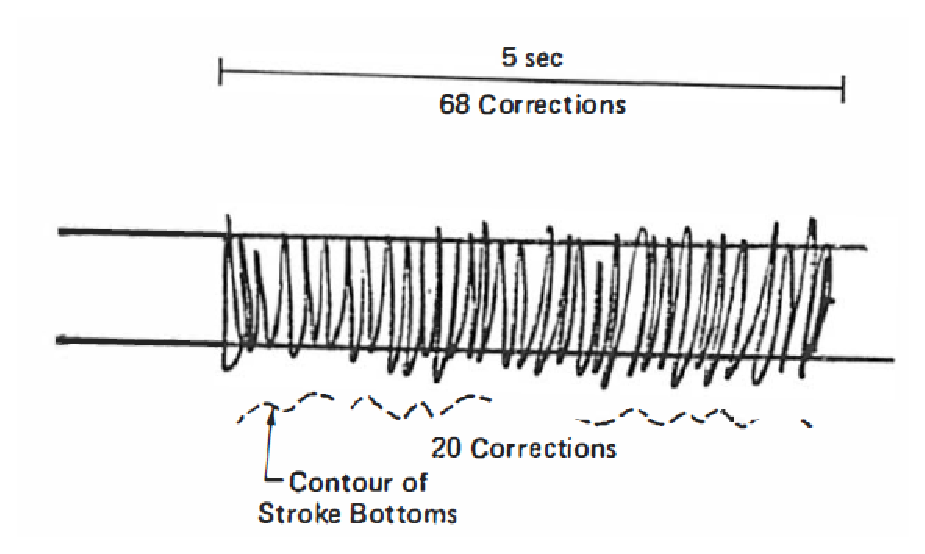
\includegraphics[width=0.5\hsize]{zigzag.eps}
 \end{center}
 \caption{�W�O�U�O�^���̎����i�}��[Wiley, 1978]��p.35���}
 \label{fig:zigzag}
\end{figure*}

����A�w�̏ꍇ�̓L�[�{�[�h���g��������������A
�u�����L�[��A�����đłv�Ƃ��������ł́A����180[ms]/�Łi���̉^��������90[ms]; �����グ�Ɖ��������j�������ł�[Wiley, 1978]�B
����͕b�ԑŌ��Ɋ��Z����Ɩ�5.6��/�b�ƂȂ�܂��i�����܂œ����L�[�A�ł̏ꍇ�ł��j�B

����𐮗�����ƁA�\\ref{tbl:renzoku}�̂悤�ɂȂ�܂��B

\begin{table*}
\begin{center}
\caption{�A���^���ɂ����鏊�v����}
\begin{tabular}{ccc}
\hline
���M�̃W�O�U�O & 70[ms] (30�`100[ms]) & 14��/�b \\
�r�E���E��̌J��Ԃ� & 100[ms] & 10��/�b \\
�L�[�{�[�h ����L�[�A�� & 180[ms] & 5.6��/�b \\
\hline
\end{tabular}
\label{tbl:renzoku}
\end{center}
\end{table*}

\subsubsection*{�t�B�b�c�̖@��}

�ȏ�̂悤�Ȓm���𗘗p���ă��f���𗧂Ă邱�Ƃ��ł��܂��B
���܁A����$D$�̏ꏊ�ɕ�$S$�i���͈ꎟ���̉^���݂̂��l���܂��B
�‚܂�A�c�����ɂ͖����ɐL�тĂ�����̂Ƃ��܂��j�̕��̂�����Ƃ��܂��B
���̕��̂ɘr�E�w�𓮂����ĐG���A�Ƃ����^�X�N���l���܂��i�}\ref{fig:fitts}�j�B

�u�ڕW���ɑ΂��Ęr�E�w�𓮂����ĐG���v�Ƃ�������͈ꓮ��Ɍ����܂����A���͂����‚��̗��U�I�ȉ^���̘A������Ȃ��Ă��܂��B
�‚܂�A�Ώە��Ƃ̋������v��Ȃ��班�����‰��x�����x���t�B�[�h�o�b�N�����A��������������Ȃǂ����Ă��܂��B

\begin{figure*}[htbp]
 \begin{center}
  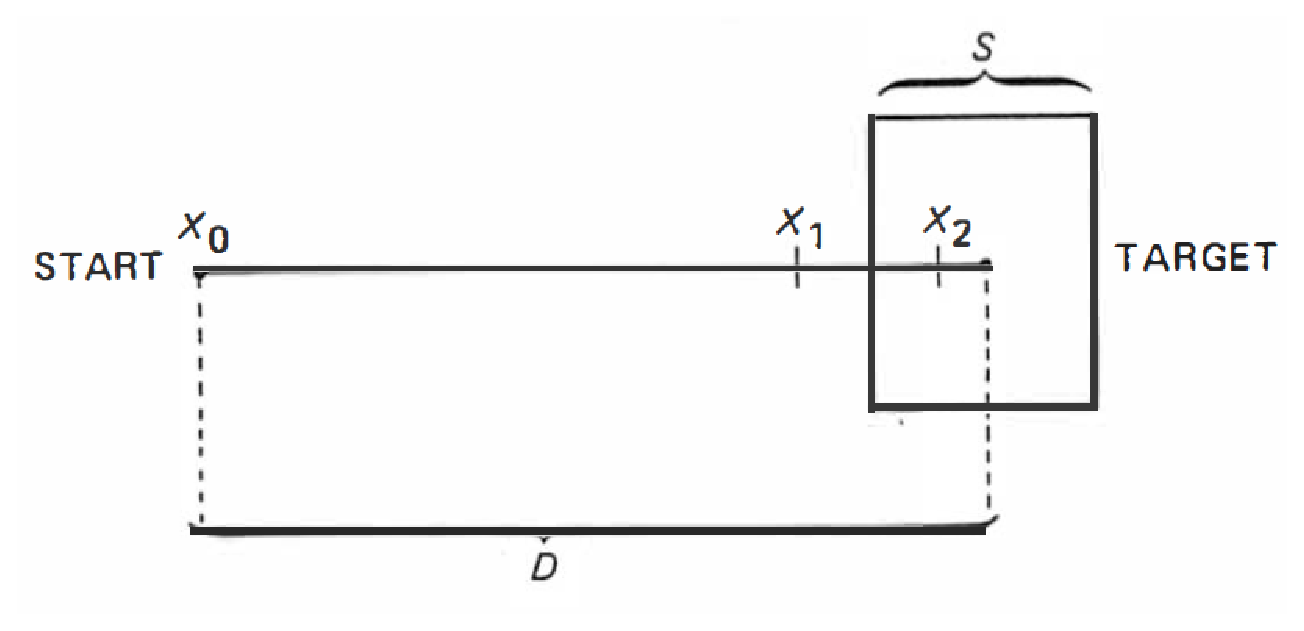
\includegraphics[width=0.5\hsize]{fitts.eps}
 \end{center}
 \caption{�t�B�b�c�̎���}
 \label{fig:fitts}
\end{figure*}

��������͐��I�ɂȂ�̂œ��o�̓R�����ɔC����Ƃ��āA���̃^�X�N�Ə��v����$T$[ms]�̊ԂɁA���̂悤�Ȗ@���������܂��F
\[
  T = I_M \log_2 \left(\frac{D}{S} + 0.5\right)
\]
�����ŁA$I_M$��100 [ms/bit]�ł�\footnote{$\log$�̒��͖������Ȃ̂ŁA�ꌩ�������Ɍ����܂����A$\log$�͒�A�‚܂�$\log_{e}$�Ȃ̂�$\log_{10}$�Ȃ̂�����ʂ��邽�߂ɁA���ʂɒP�ʂ��‚��܂��B2���Ƃ���ꍇ�́Abit���‚��܂��B���Ȃ݂ɑO��$e$��\ruby{nat}{�i�b�g}�A$10$��\ruby{dit}{�f�B�b�g}�ƌ����܂��B}%
�i70�`120�j�B

�����I�ɂ́A����Ȋ����̐����ɂȂ�܂��B�����������Ƃ���ɂ���i��$D$���ƂĂ��傫���j��$T$�͑傫���Ȃ�܂��B
����A�Ώە����������傫���i��$S$���ƂĂ��傫���j�ƁA���R�G��₷���̂�$T$�͏������Ȃ�A�‚܂葬�������܂�
�i�\\ref{tbl:fitts2}�j�B

\begin{table}[htbp]
 \begin{center}
 \caption{�t�B�b�c�̖@��}
 \begin{tabular}{ccccc}
 \hline
  & {\bf\LARGE �߂�} & $\cdots$ & {\bf\small ����} \\
  & \multicolumn{3}{c}{�Z���� $\Longrightarrow$ ������} \\
  & {\bf\LARGE �ł���} & $\cdots$ & {\bf\small ������} \\
 \hline
  \end{tabular}
  \label{tbl:fitts2}
\end{center}
\end{table}

%\begin{itembox}{{\bf �R�����@�t�B�b�c�̖@���̓��o}}
\subsubsection{�i���W�F�t�B�b�c�̖@���̓��o�j}

\hspace{1zw}
�u�Ώە��Ƃ̋������v��Ȃ��瓮�����v���U�I�ȓ����1�T�C�N���ƒ�`���܂��B���̂Ƃ��A1�T�C�N�����Ƃ�
\[
  T_{cycle} = T_p + T_C + T_M \simeq 240 {\mathrm ms}
\]
�̎��Ԃ�������܂��B$T_p, T_C, T_M$�͑O�ɒ�`�����l�ł��B
$n$�T�C�N���őΏە��ɓ��B����Ƃ���ƁA���v����$T$��
\[
  T = n \cdot T_{cycle} = n ( T_P + T_C + T_M )
\]
�ƂȂ�܂��B

�����ŁA$i$�T�C�N���ڂł̑Ώە��ւ̋�����$X_i$�Ƃ��܂��B$X_0 = D$�ł��B1�T�C�N�����Ƃɐ��䂷�鐳�m���͕ς��Ȃ��Ɖ��肷��ƁA
���鐔$\epsilon < 1$��p����$X_i = \epsilon X_{i-1}$�ƕ\�����Ƃ��ł��܂��i{\bf ��}�ł͂Ȃ�{\bf ��}���g���̂��|�C���g�ł��j�B

����ƁA���B���̑Ώە��ւ̋���$X_n$�i���̎��_�łقƂ�ǃ[���ɋ߂��Ȃ��Ă���j��
\[
X_n = \epsilon^n D
\]
�ƕ\���܂��B���ꂪ��$S$�Ɏ��܂��Ă���΁i���ڐG���Ă���΁j�悢�̂ł����A�u�s���߂��i$+S/2$�j�v�Ɓu�s������Ȃ��i$-S/2$�j�v������̂�$1/2$���܂��B�‚܂�A
\[
  \epsilon^n D \le \frac{S}{2}
\]
�����n�ɂ‚��ĉ����ƁA
\[
  n = -\log_2 (2D/S) / log_2 \epsilon
\]
����$n$��$T$�̎��ɑ�����邱�Ƃɂ���āA
\[
  T = I_M \log_2 (2D/S) \quad \mathrm{[ms]}
\]
�𓾂܂��B�������A$I_M = -(T_P + T_C + T_M) / \log_2 \epsilon$�ł��B

�萔$\epsilon$�͂�������0.07�Ƃ���Ă��܂��i[Keele,1968][Vince,1948]�j�B�����$I_M$�́A
\begin{eqnarray*}
I_M &=& -240 / \log_2 (0.07) \\
    &=& 63 \quad \mathrm{[ms/bit]}
\end{eqnarray*}
�ƂȂ�܂��B
\begin{flushright}
��
\end{flushright}
%\end{minipage}
%\end{itembox}

\subsubsection*{���K�̌��� --- �ׂ��摥}

���āA�����܂Ń��f���𗧂ĂČv�Z���Ă����킯�ł����A�l�Ԃ͂Ȃɂ��Ƃɂ���B���܂��B�‚܂�A���K���d�˂邱�Ƃɂ���āA�L�[�{�[�h�������ł‚��Ƃ��ł��܂��B

[Snoddy,1926]�́A�u���̂�m�o���Ă���^�������鎞�ԁv�Ɨ��K�ʂ̊ԂɎ��̊֌W�����o���܂����iPower Law of Practice�j�B
������{\bf �u�ׂ��摥�v�iPower Law�j}�Ƃ��Ēm���Ă���@���ł��B
\[
  n��ڂ̎��s�ɂ����鎞�� T_n = T_1n^{-\alpha}
\]
�������A$\alpha$�͂���萔�ł��B

�킩��₷�����邽�߂ɁA$\alpha=1$�Ƃ��Ă݂܂��傤�B�‚܂�A$T_n = T_1/n$�ł��B���̏ꍇ�A2��ڂ̎��s�ōŏ��̎��s�̔����A3��ڂŎO���̈�A4��ڂŎl���̈�ƂȂ�܂��B�O���t�ɕ\���Ɣ����̃O���t�ɂȂ�܂��B{\bf �ŏ��̂ق��ł����ƃ^�C�����k�܂�A��̂ق��ł̓^�C���̏k�܂�͐L�єY��ł���}���Ƃ��킩��܂��ˁB

������킩��₷���}�������̂��A�}\ref{fig:powerlaw}�ŁA$y=1/\sqrt{x}\ (=1/x^{0.5}),\  y=1/x,\  y=1/x^2$�̃O���t�ł��B��̎��ł����ƁA���ꂼ��$\alpha = \frac{1}{2}$�i�����j�A$\alpha = 1$�i�j���j, $\alpha = 2$�i�_���j�̏ꍇ�ł��B
$\alpha$���������i�������ɂȂ��Ă����j�ƁA�Ȃ��Ȃ��^�C�����k�܂�ɂ����i���c����������ɂ������^�C�����k�܂�ɂ�������B���ɂ����j���Ƃ��킩��܂��ˁB

\begin{figure*}[htbp]
 \begin{center}
  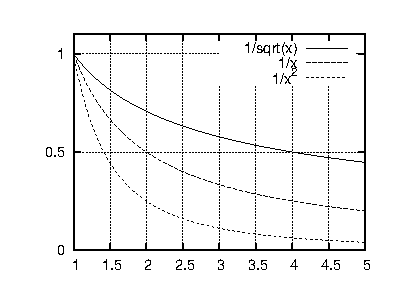
\includegraphics[width=0.7\hsize]{graph.eps}
 \end{center}
 \caption{�ׂ��摥�̗�i$y=1/\sqrt{x}$�A$y=1/x$�A$y=1/x^2$�̃O���t�j}
 \label{fig:powerlaw}
\end{figure*}

���ɋ���������ł́A$\alpha = 0.38$�Ƃ����l�������Ă��܂��B
�i��ŋ�����$1/\sqrt{x}$��������ɏ�B���ɂ����I�j

�ڂ����������܂��傤�B
�}\ref{fig:powerlaw2}��[Klemmer,1962]�ɂ������̃O���t�ł��B
Klemmer�́A�팱�҂�10�‚̃{�^���i$2^{10} =1024$�ʂ�j�̃p�^�[������K�����܂����B

\begin{figure*}[htbp]
 \begin{center}
  \includegraphics[width=0.85\hsize]{powerlaw2.eps}
 \end{center}
 \caption{�L�[���͂ɂ����� �ׂ��摥�̎����i�}��[Wiley, 1978]��p.59���}
 \label{fig:powerlaw2}
\end{figure*}

�}\ref{fig:powerlaw2}���ڂ������Ă݂܂��傤�B���ΐ��O���t�ɂȂ��Ă���̂ł킩��ɂ����ł����A���Ƃ���{\bf 1000ms����900ms�܂�100ms�k�߂�̂�1000����K���Ă���}���Ƃ��A������O�ԖڂƎl�Ԗڂ̓_����킩��܂��B���_�͂�������1000�񂲂Ƃ̗��K��\���Ă��܂��B
�܂��A$x$����10,000�̉E���A10000��ڂ���20000��ڂ̊ԂɁA�_�����W���Ă���̂������܂��ˁB����́A{\bf 600ms����500ms�܂�100ms�k�߂�̂�10000�����������}�Ƃ������Ƃ�\���Ă��܂��B1000ms��900ms�Ɣ�ׂ�{\bf 10�{�����K�ʂ��K�v}�Ƃ����̂��킩��܂��B

���̂悤�ɁA����$n$�i�����ł͗��K�񐔁j�ɑ΂��āA�Ή�����֐�$T(n)$�i�����ł̓^�C��$T$�j��$1/n$�ɔ�Ⴗ�邱�Ƃ��A{\bf �ׂ��摥}�ƌ����܂��B\footnote{�]�k�ł����A���R�E�ɂ͂��̂悤�ɂׂ��摥�����������܂��B���Ƃ��΁A���镶�͒��̒P���p�x���i�������j�ɕ��ׂ��Ƃ��ɁA��$n$�ʂ̒P��̕��͒��ɐ�߂銄����$1/n$�ɂقڔ�Ⴕ�܂��i{\bf Zipf�i�W�t�j�̖@��}�j�B���ہAthe�͕�������7\%���߁A����of�����̔�����3.5\%���߂܂��B}

\subsubsection*{�^�C�s���O���x�̗��_�Ǝ���}

�����܂ŏo�Ă����m���ŁA�^�C�s���O���x�̗��_�l���v�Z���Ă݂܂��傤�B

���̂�������������ƌv�Z���܂��B�u���M���Ђ����瑬���㉺�����ăW�O�U�O��ɏ����v�Ƃ�������ő��肵���v���l$T_M = 30 \sim 100$[ms]��p���܂��B�L�[�������̂ɂ́u���������{�����グ�v�̓񓮍삪����܂�����A$2\times T_M$�ƂȂ�܂��B
�������A���E���݂ɉ�������/�����グ���J��Ԃ��̂ŁA���ǂ̂Ƃ��뗝�_�l��$T_M$�ƂȂ�A%
{\bf �b��33�Ō��`10�Ō��i����14�Ō�/�b�j}�ƂȂ�܂��B���ۂɂ͒m�o�ɂ�锻�f�������Ă��܂��̂ŁA�����33�Ō��͕s�”\�ł��傤�B

���ۂ̂Ƃ���ǂ̂��炢�܂ő����Ȃ�̂ł��傤���H

�\\ref{tbl:speed}�ɁA�^�C�v���C�^�ł̈�X�g���[�N������̎��Ԃ������܂�\footnote{���܂��ő��ɂ��ڂ��܂����B�\�̒l��[Wiley, 1978]�ɂ��܂��B}�B�����ɂ��{\bf �^�C�s���O�`�����s�I����60[ms/��]�ŁA�����16.7[��/�b]�ɑ������܂�}�B�^�C�v�E�F������R��p�P��i400�Ō��j����{\bf 24�b}�őł����邱�Ƃ��ł��鎎�Z�ɂȂ�܂��B

\begin{table*}[htbp]
 \begin{center}
     \caption{�^�C�v���C�^�ɂ�����Ō����x}
 \begin{tabular}{lcc}
\hline
�^�C�v���C�^ & [ms/��] & �b�ԑŌ���[��/�b] \\
\hline
Best case(�`�����s�I��) & 60 & 16.7 \\
�e�L�X�g�^�C�s���O & 158�`231 & 4.3�`6.3 \\
�e�L�X�g�^�C�s���O�i�����_���P���j & 200�`273 & 3.7�`5 \\
�e�L�X�g�^�C�s���O�i�����_��������j & 462�`500 & 2�`2.2 \\
�A���t�@�x�b�g�菑�� & 545�`932(ms/��)  & 1.1�`1.8 \\
\hline
 \end{tabular}
 \label{tbl:speed}
 \end{center}
\end{table*}

\subsubsection{�e�L�[���Ƃ̎���}

�L�[�{�[�h���͂̑������A���������ڂ�����������������܂��B�}\ref{fig:kinkead1}��QWERTY�L�[�{�[�h�ɂ�����e�L�[�́A
\begin{itemize}
 \item ����Ō�
 \item �َ�Ō�
 \item ���w�Ō�
 \item ���L�[�A��
\end{itemize}
�̎l��ނ��ꂼ��̏������őł����Ƃ��ɂ����鎞�Ԃ������Ă��܂�[Kinkead,1975]�B

��Ƃ��Ĉ�Œ��Ă݂܂��傤�B�}\ref{fig:kinkead_k}��K�̃L�[���ڂ��܂��B
����̐��l162�́A�����E��ŃL�[��ł����Ƃ��A���Ƃ���\key{O}\key{K}��ł����Ƃ���\key{K}��ł‚̂ɂ����鎞�Ԃ�\���Ă��܂��B
���l�ɁA�E��̐��l133�́A����őO�̃L�[��ł����Ƃ��A�Ⴆ��\key{C}\key{K}��ł����Ƃ���\key{K}��ł‚̂ɂ����鎞�Ԃ�\���Ă��܂�
�i{\bf ����Ō��������ݑŌ��̂ق�������}�A�Ƃ������Ƃ����ĂƂ�܂��ˁj�B

\begin{figure*}[tbp]
 \begin{center}
  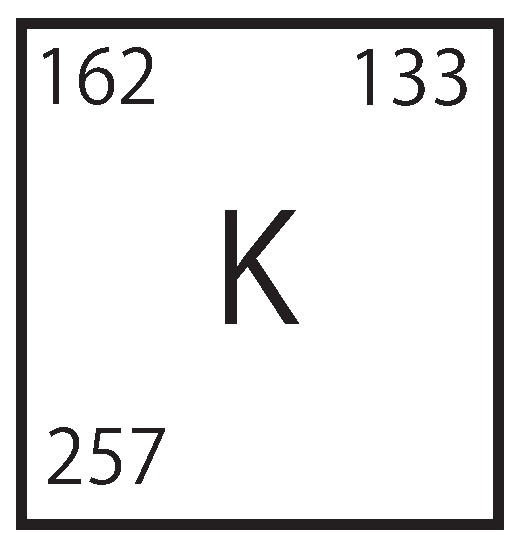
\includegraphics[width=0.15\hsize]{kinkead2.eps}
 \end{center}
 \caption{Kinkead�ɂ��L�[���͊Ԃ̑Ō����ԁAK�̗�}
 \label{fig:kinkead_k}
\end{figure*}

\begin{figure*}[htbp]
 \begin{center}
  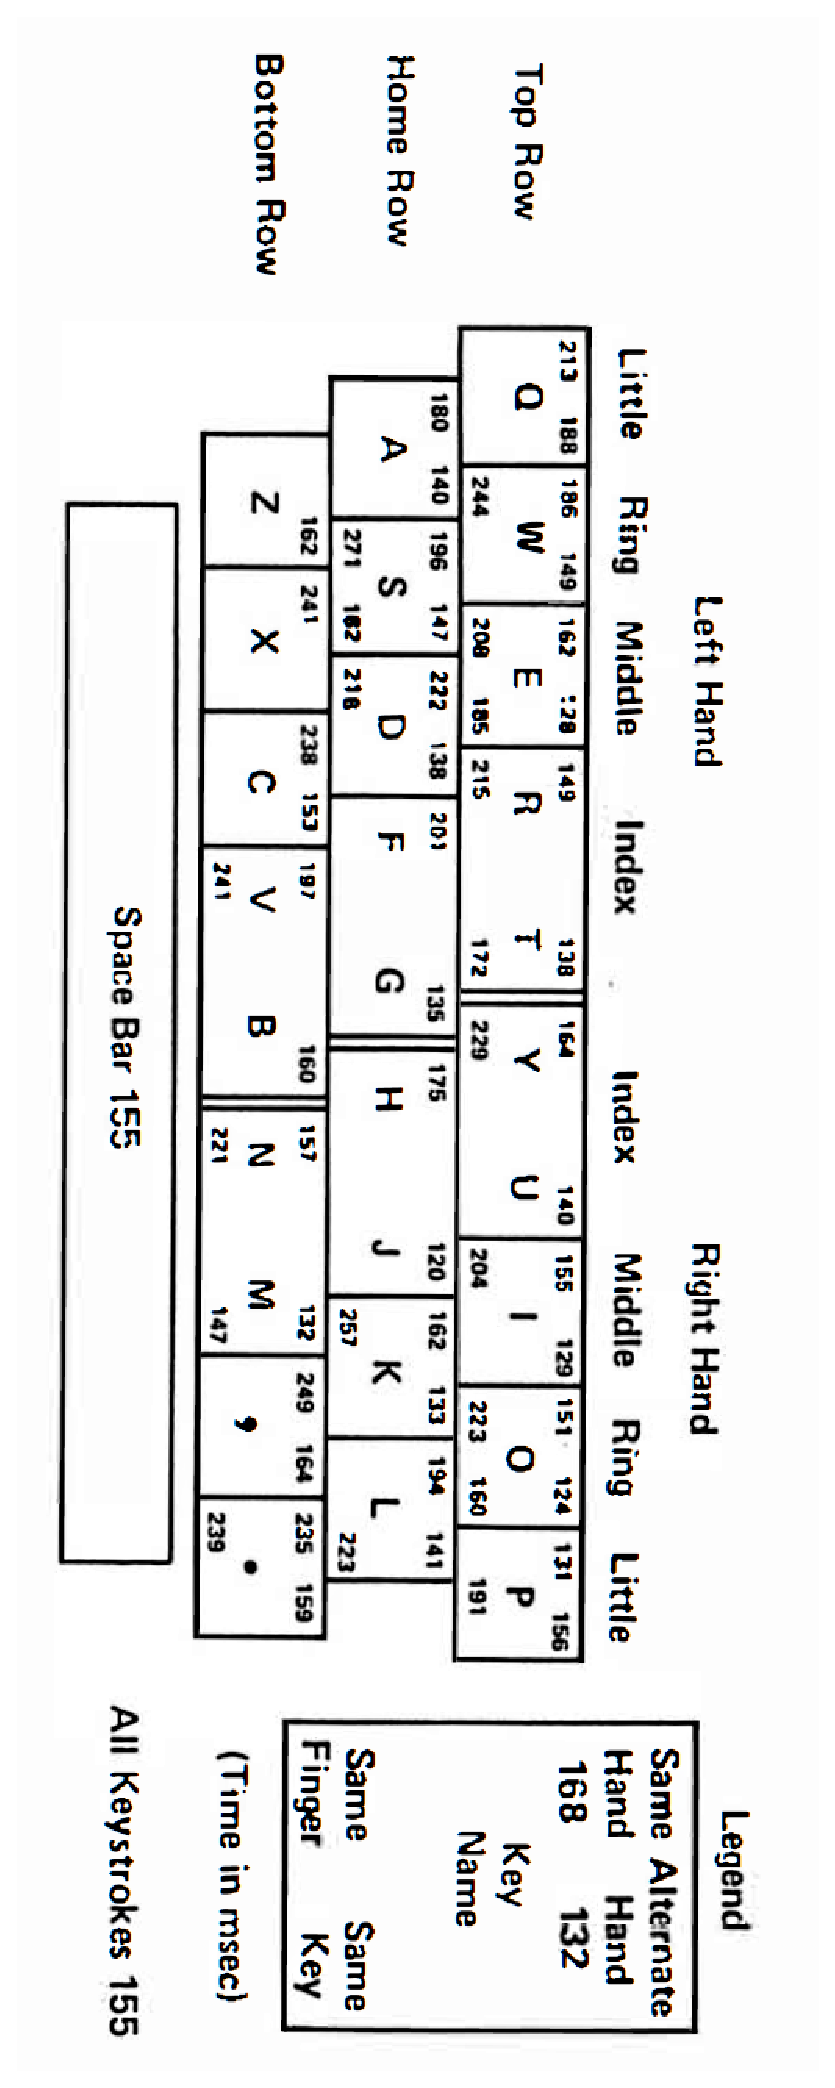
\includegraphics[height=0.9\vsize]{kinkead.eps}
 \end{center}
 \caption{Kinkead�ɂ��L�[���͊Ԃ̑Ō����ԁi�}��[Wiley, 1978]��p.62���}
 \label{fig:kinkead1}
\end{figure*}

Kinkead(1975) �͐}\ref{fig:kinkead1}�̕\�̐��l�ƁA���ۂ̉p��̕����̏o���p�x��p���āA�^�C�s���O���Ԃ𐄌v���܂����B
��̓I�ɂ́A2�����̘A�ځibigram�j�̕p�x��p���āA
\[
  \mathrm{Typing rate} = \sum_i f_i t_i
\]
�ƌv�Z���܂����B�������A$f_i$��bigram�̏o���p�x�A$t_i$��bigram�ɑΉ�����}\ref{fig:kinkead1}�̐��l�ł��B
���̌v�Z�ɂ��AKinkead��QWERTY�̃^�C�s���O���x��162ms/�łƐ��肵�܂����B�b�ԑŌ��Ɋ��Z�����6.2��/�b�ƂȂ�܂��B
Kinkead�͓����v�Z��Dvorak�ɂ‚��Ă��s���AQWERTY�ɔ�ׂ�2.6\%���������Ȃ��Ă��Ȃ��Ƃ������Ƃ������܂����B

�^�C�s���O���x�̃V�~�����[�V�������A���̂悤��bigram�̓��͑��x�̑��a�ŋߎ�����Ƃ�����@�́A�ÓT�I�ł����z��݌v�̍œK���ɖ𗧂‚ƌ����܂��傤\footnote{�������AKinkead�̃V�~�����[�V�������ʂ́u���^�w�͗lj^�w�Ɉ��e�����y�ڂ��Ȃ��v�Ƃ�������������Ă��܂��B�����[Yamada, 1980a][Yamada, 1980b]�̎����ɂ���Ĕے肳��Ă��܂��B����͎��Ԃ��Ȃ������̂ł܂�����B}�B

\section{�z���͕�}

\subsection{�͂��߂�}

���̏͂ł́A���̒��ɑ��݂����X�̔z��̂��������‚����s�b�N�A�b�v���āA�����ɂ‚��Ē�ʓI�ȕ��͂����݂܂��B
��̓I�ɂ́u���Ō����v�u���Ō����̂����A���E�E�̐��E�����v�u�V�t�g���v�u����E�E��̊e�w�ɂ�����g�p���E�䗦�v�����܂��B
�e�i�ɂ�����g�p�䗦�����܂��B����͎�Ƃ��āA�z�[���|�W�V��������肪����ɂ������ǂ���������w�W�ƂȂ�܂��B
�܂��A�ł��₷���ɂ����ďd�v�Ȉ��q�ƂȂ�A�u�A�����ē����w���g���đłi���w�ٌ�; KIKI�Ȃǁj�v
�u������Œi���i�ȏ��щz���đłi���蒵��; MIMI�Ȃǁj�v
�u����̏c�̘A���i����c�A; WAZAWAZA�Ȃǁj�v�������܂��B

�ȉ���QWERTY���[�}�����͂��ɂƂ��Č��Ă݂܂��傤�i�\\ref{tbl:roma_example}�j�B

�܂���i�ڂ��A���Ō����ƁA����E�E��ł̑Ō����Ƃ��̔䗦�ł��B�V�t�g���̓V�t�g���������񐔂ŁA���ʓ��̓N���X�V�t�g�ł��iNICOLA�z��A���w�V�t�g�z��Ō����Ă��܂��j�B�E���́u����/����/�E�E�v�́A�񕶎��Ԃł̎�̓��������������̂ł��B
��i�ڂ͊e�w�̎g�p�䗦�ƂȂ��Ă��܂��B�����獶���w�A��w�A�c�c�A�E���w�ƂȂ��Ă��܂��B
�O�i�ڂ͐�s�����ŋc�_����Ă���u�����w�ňႤ�L�[��A���őłi���w�ٌ��j�v�u������Œi���i�ȏ��щz����L�[��łi���蒵��j�v�u����ŘA�������c�̃L�[��łi����c�A; \key{Z}\key{A}�Ȃǁj�v�̎g�p���A����ъe�i���Ƃ̎g�p�䗦�ƂȂ��Ă��܂��B


\begin{table*}[htbp]
 \caption{QWERTY���[�}���̉�͕\}
 \begin{center}
 \begin{tabular}{cccc|ccc}
 \hline
���Ō� & ���Ō��� & ���Ō��E & �V�t�g�� & ���� & ���� & �E�E \\
37818164 & 16102479 & 21715685 & 7216(7216) & 17753448 & 7225755 & 12838961 \\
 & 42.6\% & 57.4\% & & 46.9\% & 19.1\% & 33.9\% \\
 \hline
 \end{tabular}

 �@\vspace{1zw}�@

 \begin{tabular}{ccccccccccc}
 \hline
& ����(A) & ����(S) & ����(D) & ���l(FG) & �E�l(HJ) & �E��(K) & �E��(L) & �E��(;)\\
& 5180235 & 2405277 & 3120281 & 5396686 & 9531741 & 7001152 & 4679026 & 503766\\
��/�E�蒆 & 32.2\% & 14.9\% & 19.4\% & 33.5\% & 43.9\% & 32.2\% & 21.5\% & 2.3\%\\
���Ō��� & 13.7\% & 6.4\% & 8.3\% & 14.3\% & 25.2\% & 18.5\% & 12.4\% & 1.3\%\\
\hline
 \end{tabular}

 �@\vspace{1zw}�@

 \begin{tabular}{ccc|cccc}
 \hline
 ���w�ٌ� & ���蒵�� & ����c & �ʼn��i(ZX..) & �z�[��(AS..) & �O�i��(QW..) & �ŏ�i(12..)\\
 2991366 & 5170649 & 3457 & 6024198 & 12333179 & 19265593 & 195194\\
  &  &  & 15.9\% & 32.6\% & 50.9\% & 0.5\%\\
%����/����/�E�E �� & ����/����/�E�E �� & ����/����/�E�E �� &  &  &  & ���Ō��� & ���Ō��� & ���Ō��� & ���Ō���\\
\hline
 \end{tabular}
 \end{center}
 \label{tbl:roma_example}
\end{table*}

\subsection{QWERTY�ɂ‚���}

�܂��i���I�ȁj�e�z��Ɉڂ�O�ɁA�������i��ł���QWERTY�ɂ‚��Č��Ă݂邱�Ƃɂ��܂��B���̌�AAZIK�A���Ȕz��ƌ��Ă����܂��B

\subsubsection*{QWERTY�́u�ł��₷���v���H}

�݂Ȃ��񂪂����΂�ڂɂ��邱�Ƃ̑����z��AQWERTY�̓^�C�v���C�^�[�̔z��Ɏn�܂�܂��B1868�N�ɂ̓A���t�@�x�b�g�����̂܂ܕ��ׂ����̂ł������^�C�v���C�^�[�̔z�񂪁A���݂�QWERTY�z��Ɠ������̂ɂȂ����̂́A1882�N8���̂��Ƃł��i�����F���w�L�[�{�[�h�z��QWERTY�̓�x�ANTT�o�ŁA2008�N�j�B

QWERTY�L�[�{�[�h�ɑ΂���ᔻ�͐���������A�܂�����炪���̔z����l�Ă����铮�@�ɂ��Ȃ��Ă��܂��B
�i1983�N�����́j�ߋ�50�N�Ԃɂ�����QWERTY�z��ɑ΂���ᔻ���܂Ƃ߂��%
%\footnote{��Ƃ���Dvorak���m�Ƃ��̃`�[���ɂ��ᔻ�ł���[Dvorak, 1943]�BDvorak���QWERTY�z��ᔻ������ŁAFIXME}%
[Noyes, 1983]�A

\begin{enumerate}
\item ����ɉߕ��ׂł���B�L�[�̎��s��57\%���A�����̐l�������r�łȂ�����ɂ��s����%
    \footnote{����͉p��̏ꍇ�ł��邱�Ƃɒ��ӂ��Ă��������B���{��̏ꍇ�͂���ƈقȂ�܂��B�ڂ����͌�q�̃��[�}�����͂ŁB}
\item ����w�ɂƂ��ĉߕ��ׂł���\footnote{�@�B���̃^�C�v���C�^�ł́A�S�Ă̎w�œ����͂��g���ē��͂���K�v������܂����B���̂��߁A���w���w�ȂǁA�͂̎ア�w�ɕ��S�������邱�Ƃ��������悤�ł��B�d�����ɂȂ��Ă���A���̌��_�͂��قǖ��ł͂Ȃ��Ȃ�܂����B}
\item ���i�̃L�[�̎��s�����Ȃ����i32\%�j�A��i�̃L�[�̎��s����������i52\%�j
\item �悭�g�p�����P��ɂ����āA�i�̕ύX����������B���΂��Ή��i�A��i�A���i�ƂȂ邱�Ƃ�����B���Ƃ��� ``br, un, in''�ȂǁB
\item �����̈�ʗp�ꂪ���肾���Ń^�C�v�����B���Ƃ��� ``was, were, extra, address''
\end{enumerate}

���̂���3�Ԗڂ͕⑫���K�v�ł��B[Kinkead, 1975]�ɂ��ƁA�@�B���̃^�C�v���C�^�ł͒��i�̃L�[�������̂��ł������A�d�C�I�ȃ^�C�v���C�^�[�ł͏�i�̃L�[���삪�ł������Ƙ_���Ă��܂��i�n�������^�C�s�X�g�ɂ������j�B

\subsection{QWERTY���[�}������}

���āA��������͓��{��^�C�s���O�ɂ‚��ċc�_���Ă������Ƃɂ��܂��B
�܂��́A�����炭��ԕW���I�ȓ��͕����ł��郍�[�}�����͂���B

QWERTY���[�}�����͂��R�[�p�X��p���ĕ]������ƕ\\ref{tbl:roma}�̂悤�ɂȂ�܂��B

���{��̃^�C�s���O�ɂ����ẮA�O�q��Noyes�̎咣�i����Ώd�j�ɑ΂��āA
�E��Ώd�̔z��ɂȂ��Ă��邱�Ƃ����������܂��B
���ɁA�E��l�����w�̎g�p�������̔z��Ɣ�׍����Ȃ��Ă��܂��B

���́A�E��Ώd�E�E��l�����w�Ώd�̌��ʂɂ‚��ẮA���̓_�������Ƃ��čl�����܂��B
\begin{itemize}
\item ���{��́u�q���{�ꉹ�v�ňꕶ���ƂȂ邪���̂����E��őł•ꉹ�i\key{I}\key{O}\key{U}�j���ꉹ���̖�6�����߁A����ɔ�ׂĂ�⑽�����ƁA
\item �悭�o�鉼���̎q�����A�E��l�����w�ɏW�����Ă��邱�ƁA
\item[�@] \hspace{1zw}�i�p�x���ɋ�����ƁA�u%
{\footnotesize ��}%
\ruby{{\bf ��}}{U}%
\ruby{{\bf ��}}{N}%
{\footnotesize ��}%
\ruby{{\bf ��}}{N}%
{\footnotesize ������}%
\ruby{{\bf ��}}{N}%
{\footnotesize ��}%
\ruby{{\bf ��}}{N}%
\ruby{{\bf ��}}{H}�v�̑����j�B
\end{itemize}

����A����̕��͍����w�̍��g���Ђǂ��A���̔z��ɔ�׌Q�𔲂��Ă��܂��B�u\ruby{��}{����}��iSASAZAWA�j�v�Ȃǂ́u��v���t���l����A�u�킴�킴�iWAZAWAZA�j�v�̑ł��ɂ����́A�����̐l���o�����Ă��邱�ƂƎv���܂��B

%\begin{table}[htbp]
% \begin{center}
%  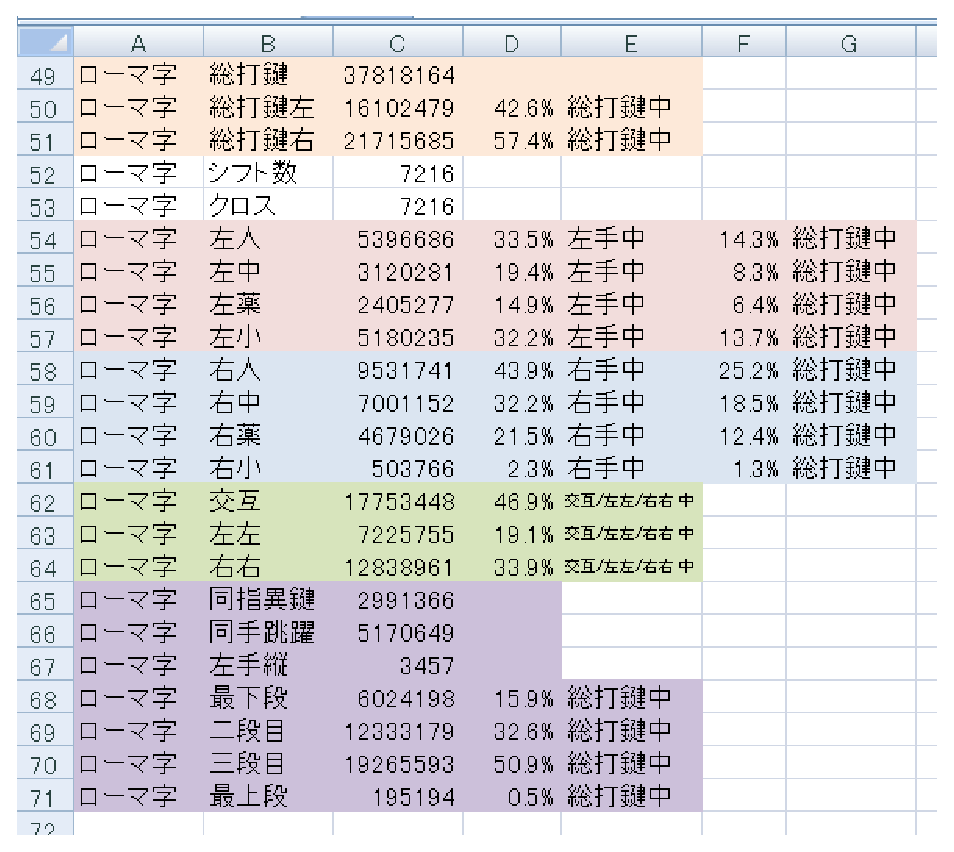
\includegraphics[width=0.85\hsize]{tbl-roma.eps}
% \end{center}
% \caption{QWERTY���[�}���̉�͕\}
% \label{tbl:roma}
%\end{table}

\subsection{AZIK}

QWERTY�ɂ�郍�[�}�����͂��������ǂ����̂��AAZIK�ł��B
AZIK�ł́A���{��̊����̉��̑������u���v�u��v�u���v
�i�u\ruby{��}{����}�v�u\ruby{��}{����}�v�u\ruby{��}{����}�v�Ȃǁj�ŏI��邱�Ƃɒ��ڂ��܂����B
��萳�m�Ɍ����΁A���[�}���ŏ����āA-ai�A-an�A-ou�Ȃǂ̉��ŏI��镶���������A�Ƃ������Ƃł��B
������AZIK�ł́A����``ai''�A``an''�ɁA�ꕶ�������蓖�Ă邱�Ƃɂ��܂����B
���Ƃ���``ai''��\key{Q}�A``an''��\key{Z}�ł��B���{��ł́A�q���ƕꉹ�����݂ɘA�Ȃ邱�Ƃ���u�q���{�q���v�̑g�ݍ��킹�ɂȂ����Ƃ��i���Ƃ���``KZ''�j�̂�
\key{Z}��an�Ɖ��߂���΁A�u�����������v�Ƌ������邱�Ƃ͂���܂���%
\footnote{����́AATOK��Google���{����͂̃��[�}���ϊ��e�[�u���ŗe�ՂɎ����ł��܂��B}�B%
���{��̊����͑S���̖͂�3�����߂܂��̂ŁA�����̊������̓��͂��ȓ��͉�����΁A�S�̓I�ȑŌ����͏��Ȃ��Ȃ�܂��B

�܂��AAZIK�ł́u���v�̕������ꕶ���i\key{;}�j�œ��͂�����A�p�o�́u����v�u���Ɓv�Ȃǂ�``sr''�A``kt''�œ��͂���ȂǁA�����ɏȓ��͉��������܂��B

���̑����M���ׂ����ƂƂ��āA����s�A�Ђ�s�A�݂�s�Ȃǂ�\ruby{�X}{�悤}���ɂ‚��āA``KYU''�Ȃǂł͂Ȃ�``KGU''�ł��łĂ�悤�ɂ��Ă���_������܂��B����͏ȓ��͉��ł͂Ȃ��A���E���ݑŌ���_�������ǂł��B���̂悤�Ȍ��ݑŌ���ړI�Ƃ����g���Ƃ��āA�u����v�iDZ�j��``DN''�ł��łĂ�悤�ɂ������̂�����܂��B

���āAAZIK���R�[�p�X���g���ĕ]�����Ă݂܂��傤�B
%AZIK�ɂ‚��ẮA��҂��ȓ��͉��ɒi�K��݂��Ă��܂��̂ŁA���ނ̕]���ݒ���Ƃ�܂����B��̓I�ɂ́A�uAZIK���������\footnote{{\tt http://hp.vector.co.jp/authors/VA002116/azik/azikinfo.htm}}�v�ɂ���u���̂Q�i�g���L�[�j�v�݂̂̂ƁA�u���̂R�v�܂őS�Ďg�p�����ꍇ�̓�ʂ�ł��B
�]���ɂ́A
\begin{itemize}
 \item \ruby{��}{�͂�}���g���i-an�Ȃ�, �L�[:ZNKJDL�j�i\key{Z}��\key{N}�ɂ‚��ẮA�O�߂ŏq�ׂ����ݑŌ��̗D�ʐ���\ruby{��}{����}�݂āA���ݑŌ��ɂȂ�悤�Ɋe�L�[��I�����܂����j
 \item ��d�ꉹ�g���i-ai�ȂǁA�L�[:QHWP�j
 \item �u���v�u���傤�v�Ȃ�sh�̉���\key{x}�œ��� / �u���v�Ȃ�ch�̉���\key{c}�œ���
 \item �u��v�u���v�����ꂼ��\key{Q}, \key{;}�œ���
 \item \ruby{�X}{�悤}����\key{Y}�ł͂Ȃ�\key{G}�œ���
 \item �u����v�u���Ɓv�Ȃǂ����ꂼ��\key{S}\key{R}�A\key{K}\key{T}�Ȃǂœ���
\end{itemize}
�Ƃ����ݒ��p���܂����B����́uAZIK���������\footnote{\url{http://hp.vector.co.jp/authors/VA002116/azik/azikinfo.htm}}�v�ɂ���A�u���̂R�v�܂ł̐ݒ���قړ��P���Ă��܂��B

%\begin{table}[htbp]
% \begin{center}
%  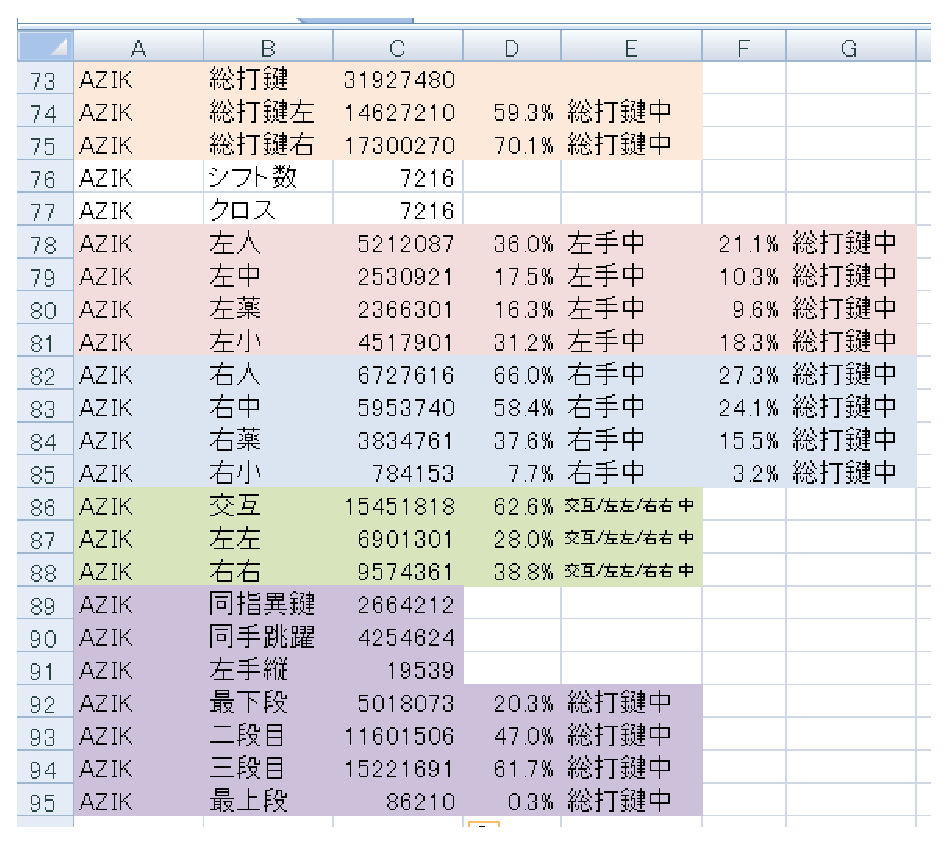
\includegraphics[width=0.85\hsize]{tbl-azik.eps}
% \end{center}
% \caption{AZIK�̉�͕\}
% \label{tbl:azik}
%\end{table}

\begin{table*}[htbp]
 \caption{AZIK�̉�͕\}
 \begin{center}
 \begin{tabular}{cccc|ccc}
 \hline
���Ō� & ���Ō��� & ���Ō��E & �V�t�g���i�N���X�j & ���� & ���� & �E�E \\
30200816 & 14072150 & 16128666 & 98014(9948) & 15211220 & 6466540 & 8523056 \\
 & 46.6\% & 53.4\% &  & 50.4\% & 21.4\% & 28.2\% \\
 \hline
 \end{tabular}

 �@\vspace{1zw}�@

 \begin{tabular}{ccccccccccc}
 \hline
& ���� & ���� & ���� & ���l & �E�l & �E�� & �E�� & �E�� \\
& 3998593 & 2366304 & 2145980 & 5561273 & 6426213 & 5422220 & 3496080 & 784153 \\
��/�E�蒆 & 28.4\% & 16.8\% & 15.2\% & 39.5\% & 39.8\% & 33.6\% & 21.7\% & 4.9\% \\
���Ō��� & 13.2\% & 7.8\% & 7.1\% & 18.4\% & 21.3\% & 18.0\% & 11.6\% & 2.6\% \\
\hline
 \end{tabular}

 �@\vspace{1zw}�@

 \begin{tabular}{ccc|cccc}
 \hline
 ���w�ٌ� & ���蒵�� & ����c & �ʼn��i(ZX..) & �z�[��(AS..) & �O�i��(QW..) & �ŏ�i(12..)\\
2030767 & 3797767 & 15170 & 5018292 & 11429889 & 13666425 & 86210 \\
 &  &  & 16.6\% & 37.8\% & 45.3\% & 0.3\% \\
%����/����/�E�E �� & ����/����/�E�E �� & ����/����/�E�E �� &  &  &  & ���Ō��� & ���Ō��� & ���Ō��� & ���Ō���\\
\hline
 \end{tabular}
 \end{center}
 \label{tbl:azik}
\end{table*}

����AZIK�́AQWERTY���[�}���i��3782�����j�ɔ�ׁA��20\%�Ō������팸�ł��Ă��܂��B����͑O�q�̓�d�ꉹ�Ȃǂ̏ȓ��͂ɉ����A���{��ŕp�o�́u����v�u���Ɓv��2�X�g���[�N�œ��͂ł���悤�ɂ������Ƃ��傫���̂ł��傤%
\footnote{���Ȃ݂�2000�����̃R�[�p�X�ł́A�u����v��57752��A�u���Ɓv��88757��o�Ă��܂����B}�B

����̎q���̃L�[�𑽗p���邱�Ƃ���A����̎g�p���͎኱�����Ȃ�܂����B
�������A\key{Q}/\key{Z}��ł‚ׂ����菬�w�ɂ‚��ẮA���[�}����13.7\%�ɔ�ׂ�AZIK��13.2\%�ƁA�قƂ�Ǖς���Ă��܂���B

AZIK�̔z�u�͊o���₷���̂��߂ɁA�Ή�����ꉹ�̃L�[�̋߂��i-ai/-an�Ȃ�\key{A}�̋߂���\key{Q}��\key{Z}�j
�Ƃ���������݂��Ă��܂����B���̂��߁A�L�[�{�[�h�z��̑ł��₷���Ƃ����ϓ_���猾���΂ނ���A
�s���Ȃ��̂ƂȂ��Ă��܂��댯���������Ă��܂��B

���ہA��ŏq�ׂ��悤�ȍH�v���g�킸�A�P����\ruby{��}{�͂�}���g���iZKJDL�j�A��d�ꉹ�g���iQHWP�j�������g����
�\�������ł́A\key{A}��\key{E}������ɂ��邱�ƁA\key{Q}��\key{Z}�����菬�w�ł��邱�ƂɈ����Â��āA
���菬�w�E��w�����g����z��ɂȂ��Ă��܂��Ă��܂����B

AZIK�́A�ȓ��͉��̕��@���ӂ񂾂�ɗp���A����Ɍ��ݑŌ��܂ōl���������ʂƂ��āA
�o���₷���ƌ����𗼕��J�o�[�����A�o�����X�̂Ƃꂽ�z��ɂȂ����A�ƌ�����ł��傤%
\footnote{�������A``sr''������A�ȊO�̔�r�I�p�x�̒Ⴂ�񕶎����o���₷�����ǂ����͋c�_�̗]�n������܂��B}�B

%������A``ai''�Ȃǂ̃L�[�͂ǂ̎q���̃L�[�ɒu���Ă��悢���߁A����ɂ‚��Ă͉��ǂ��]�߂܂�%
%\footnote{���̂��߁A�M�ҁinooyosh�j�͂���YAZIK: Yet another AZIK�Ƃ����z����l���Ă���̂ŁA����ȍ~������ҁB}�B

\subsection{JIS����}

�݂Ȃ��񂲑����́u���Ă�������Ȃɂ点�v�\�\JIS����%
\footnote{���ɐ�������u�VJIS�z��v�Ƃ̔�r�Łu��JIS�v�ƌĂ΂�邱�Ƃ�����܂��B}%
�́A�����J�i�^�C�v���C�^�̔z�񂩂�l�Ă���A1972�N��JISC 6233�Ƃ��Đ��肳��܂����B�����Ƃ��ẮA�i�قځj���ׂẴL�[�g���ĉ�����z�u���悤�Ƃ������߂ɁA�L�[���l�i���ׂĎg���Ă���_�ł��B
��q����e�w�V�t�g�⒆�w�V�t�g�Ȃǂ̂悤�ɁA�V�t�g�L�[�������K�v���Ȃ����߂ɒ����I�ł͂���̂ł����A
\begin{itemize}
\item �ォ���i�ڂ̎g�p�p�x�������A�z�[���|�W�V��������w������₷��
\item �Ō�������ɕ΂��Ă���
\item ������ł‚Ƃ��ɃJ�i�L�[�������K�v������
\end{itemize}
�ȂǁA���낢��ƌ��_������܂��B

�ڂ������Ă݂܂��傤�i�\\ref{tbl:jiskana}�j

\begin{table*}[htbp]
 \caption{JIS���Ȃ̉�͕\}
 \begin{center}
 \begin{tabular}{cccc|ccc}
 \hline
���Ō� & ���Ō��� & ���Ō��E & �V�t�g�� & ���� & ���� & �E�E \\
24675899 & 14475950 & 10199949 & 2666111(2213255) & 11525084 & 8713408 & 4437407\\
 & 58.7\% & 41.3\% &  & 46.7\% & 35.3\% & 18.0\%\\
 \hline
 \end{tabular}

 �@\vspace{1zw}�@

 \begin{tabular}{ccccccccccc}
 \hline
& ����(A) & ����(S) & ����(D) & ���l(FG) & �E�l(HJ) & �E��(K) & �E��(L) & �E��(;)\\
& 5609655 & 3528341 & 2956460 & 2381494 & 3483694 & 2418311 & 2048886 & 2249058\\
��/�E�蒆 & 38.8\% & 24.4\% & 20.4\% & 16.5\% & 34.2\% & 23.7\% & 20.1\% & 22.0\%\\
���Ō��� & 22.7\% & 14.3\% & 12.0\% & 9.7\% & 14.1\% & 9.8\% & 8.3\% & 9.1\%\\
\hline
 \end{tabular}

 �@\vspace{1zw}�@

 \begin{tabular}{ccc|cccc}
 \hline
 ���w�ٌ� & ���蒵�� & ����c & �ʼn��i(ZX..) & �z�[��(AS..) & �O�i��(QW..) & �ŏ�i(12..)\\
4885493 & 3477500 & 487390 & 4477353 & 6071650 & 10022415 & 4104481\\
 &  &  & 18.1\% & 24.6\% & 40.6\% & 16.6\%\\
\hline
 \end{tabular}
 \end{center}
 \label{tbl:jiskana}
\end{table*}

%\begin{table}[htbp]
% \begin{center}
%  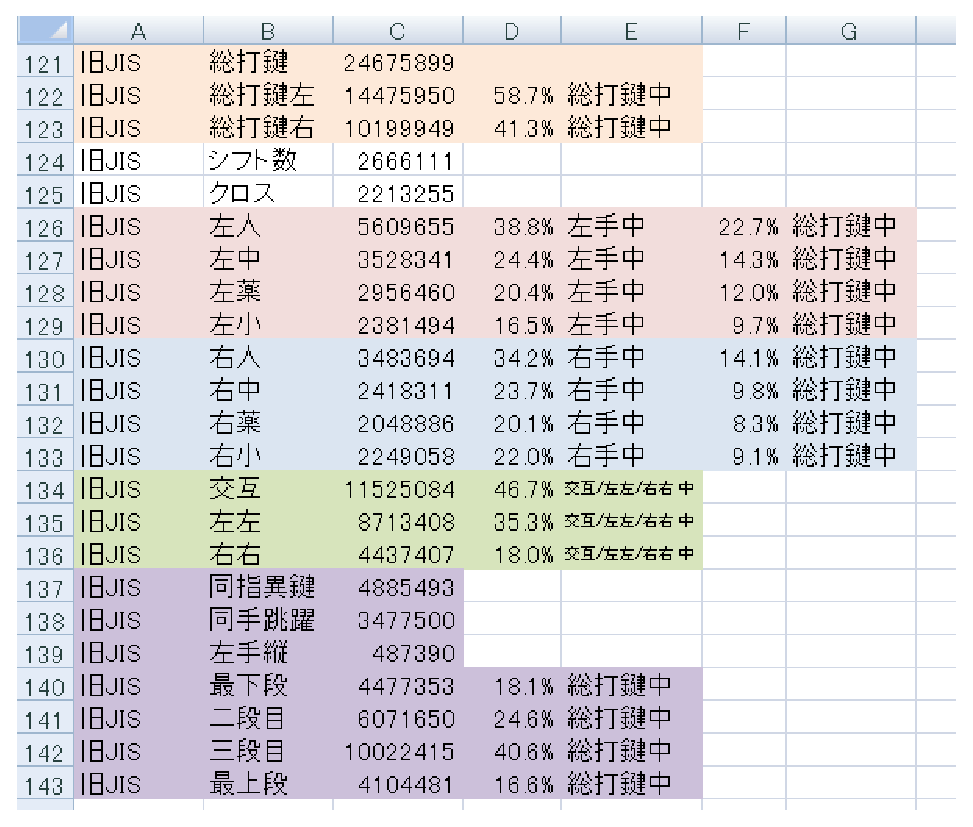
\includegraphics[width=0.85\hsize]{tbl-jiskana.eps}
% \end{center}
% \caption{��JIS�̉�͕\}
% \label{tbl:jiskana}
%\end{table}

���Ō�����6��������ɂȂ�܂��B���̂����A���l�����w�����Ō��̖�23\%���߂�ȂǁA�������΂肪�����܂��i�u���v�u���v�Ȃǂ����l�����w�̍��p�x�����j�B
bigram�A�‚܂�񕶎���̘A�Ȃ�����Ă��A���聨����̑g�ݍ��킹��4����ƁA����̍��g�����Ď��܂��i�u�Ă��v�u�����v�Ȃǁj�B
�܂��A�ォ���i�ځiQWE...�j�����Ō��̖�4�����߂�ȂǁA�z�[���|�W�V��������w������₷���_���m�F�ł��܂��B

\subsection{�VJIS�n�E���w�V�t�g�n�J�i�z��}
\subsubsection*{�VJIS}

JIS���Ȃ̌��_���������邽�߁A1986�N�ɐV���������z��JIS�Ō��肳��܂����B
����́A�u�p�x�̔�r�I�Ⴂ�L�[�̓V�t�g�œ��͂����A�w���z�[���|�W�V��������Ȃ�ׂ�����Ȃ��悤�ɂ���v�Ƃ����݌v�v�z�Ɋ�Â��čl�Ă��ꂽ�z��ł��B
��ʂɐVJIS�ƌĂ΂�܂��B
�������AJIS���Ȃ��p�~���ꂸ�ɕ����������Ƃ���A�VJIS�͑S�����y�����A�u�g�p���Ԃ��Ȃ��v�Ƃ���1999�N�ɔp�~����Ă��܂��܂����B

�VJIS�̐݌v�ł́A�L�[�{�[�h�ŏ�i�i�����L�[�̂���i�j�̓��̓X�s�[�h���A���̒i�ɔ�ׂĒx�����Ƃɒ��ڂ��܂����B
�z�[���|�W�V�������牓���L�[�̓��͂��x�����Ƃ́A�O�q�̃t�B�b�c�̖@���i�����ɂ��鏬�����L�[�قǓ��͑��x���x���j������킩��܂��B
�����ŁA�VJIS�ł͉��������ׂĎO�i�Ɏ��߂悤�Ƃ��܂����B�O�i�ł͑���Ȃ��̂ŁA�o���p�x�̒Ⴂ�����ɂ‚��Ă̓V�t�g�L�[��p���ē��͂���悤�ɂ��܂����i�u���ɔz�u�v�j�B

���ɁA�ǂ�������z�u���邩�ł��B�܂��l�������ׂ��́A�o���p�x�ł��B����Ɋւ��ẮA���Z���ȏ��̕��͂́u�P�����̏o���p�x�v�iunigram�̕p�x�j�A�u2�����̘A�ڂ̏o���p�x�v�ibigram�̕p�x�j���p�����܂����B

��̓I�ɂ́A���̂P�D����S�D�̃X�e�b�v���o�܂��B

\begin{enumerate}
\item �u�P�����̏o���p�x�v���������i�u���v�u���v�u��v�c�c�j�ɉ�������ׁA�������u�V�t�g���Ȃ��œ��͂����L�[�v�i�u�\�v; �A���V�t�g�j�ɐݒ肵�܂��B
�Ⴆ�΁A�u���v�͓��{��̕��͂ň�ԑ����o�����邽�߁A���R�\�ɏo�Ă��܂��B
\item �������A���ݑŌ������ő�ɂȂ�悤�ɍ��E�ɕ����܂����B�u���݁v�̌v�Z�ɂ́A��ł�����bigram��p���܂��B�������ł������u2�����̘A�ځv�ibigram�j���g���܂��B
    �u�Ă��v�͂ƂĂ������ibigram�S�̖̂�0.7\%�j������̂ŁA\key{��}��\key{��}�̃L�[�́i�Ȃ�ׂ��j���E�ɕ������Ĕz�u���������悢���ƂɂȂ�܂��B
\item ���E�O���[�v���ꂼ��ɂ‚��āA�w�̒i�z�������Ȃ��Ȃ�悤�ȑg�ݍ��킹��T���܂��B
\item ����ɁA���E�O���[�v���ꂼ��ɂ‚��āA�����w���A�����đłi���w�ٌ��j�񐔂����Ȃ��Ȃ�悤�ȑg�ݍ��킹��T���܂��B
\end{enumerate}

�V�t�g����鉼���̏W���ɂ‚��ẮA�V�t�g�L�[���P�X�g���[�N�ƌ��Ȃ��āA���ݑŌ��̕p�x���ő�ɂȂ�悤�ɍ��E�O���[�v�ɂ킯�A����Ƀz�[���|�W�V�����̒i�ɕp�x�̍���������z�񂷂�悤�ɂ��܂����B

������R�[�p�X���g���Č��Ă݂܂��傤�i�\\ref{tbl:newjis}�j

\begin{table*}[htbp]
 \caption{�VJIS�̉�͕\}
 \begin{center}
 \begin{tabular}{cccc|ccc}
 \hline
���Ō� & ���Ō��� & ���Ō��E & �V�t�g�� & ���� & ���� & �E�E \\
24706219 & 11010567 & 13695652 & 4031578\\
 & 44.6\% & 55.4\% & \\
 \hline
 \end{tabular}

 �@\vspace{1zw}�@

 \begin{tabular}{ccccccccccc}
 \hline
& ����(A) & ����(S) & ����(D) & ���l(FG) & �E�l(HJ) & �E��(K) & �E��(L) & �E��(;)\\
& 4738263 & 2648262 & 2256137 & 1367905 & 5212719 & 3530762 & 3702200 & 1249971\\
��/�E�蒆 & 43.0\% & 24.1\% & 20.5\% & 12.4\% & 38.1\% & 25.8\% & 27.0\% & 9.1\%\\
���Ō��� & 19.2\% & 10.7\% & 9.1\% & 5.5\% & 21.1\% & 14.3\% & 15.0\% & 5.1\%\\
\hline
 \end{tabular}

 �@\vspace{1zw}�@

 \begin{tabular}{ccc|cccc}
 \hline
 ���w�ٌ� & ���蒵�� & ����c & �ʼn��i(ZX..) & �z�[��(AS..) & �O�i��(QW..) & �ŏ�i(12..)\\
2495822 & 830701 & 38977 & 4876067 & 13254518 & 6496686 & 78948\\
 &  &  & 19.7\% & 53.6\% & 26.3\% & 0.3\%\\
\hline
 \end{tabular}
 \end{center}
 \label{tbl:newjis}
\end{table*}



%\begin{table}[htbp]
% \begin{center}
%  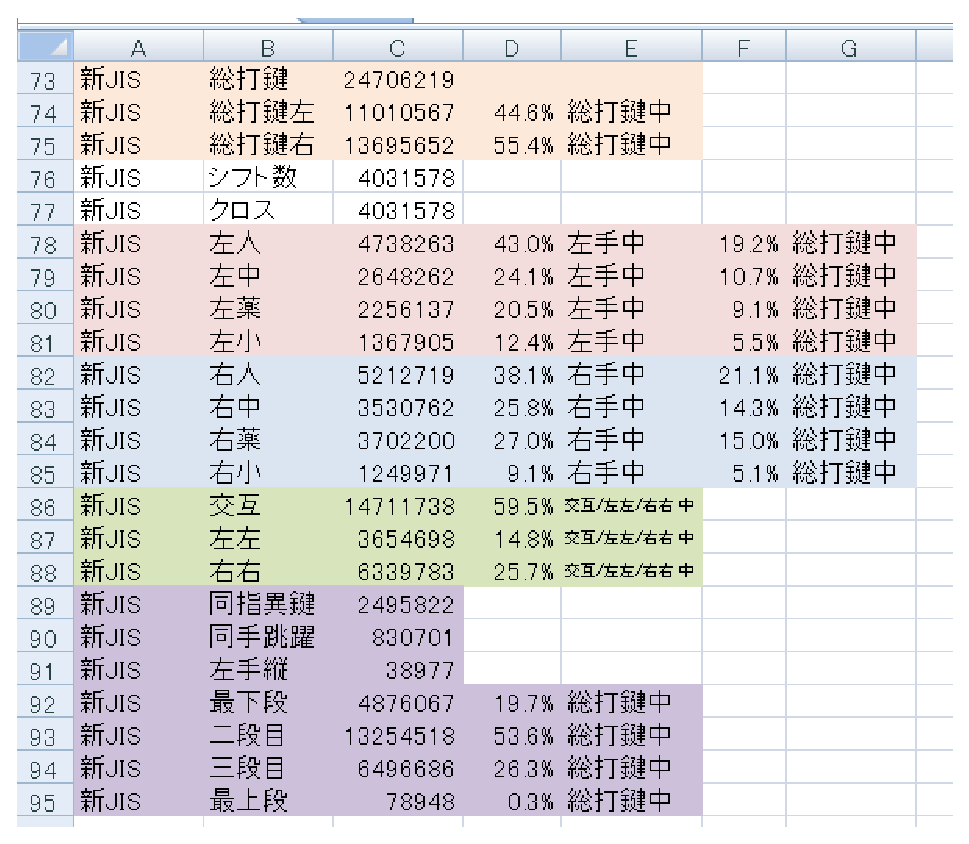
\includegraphics[width=0.85\hsize]{tbl-newjis.eps}
% \end{center}
% \caption{�VJIS�̉�͕\}
% \label{tbl:newjis}
%\end{table}

�E��ƍ����\ruby{����}{������}���኱���P����܂����B�܂��A���ݑŌ����S�̖̂�6���ƁAJIS���Ȃ̖�46\%�Ɣ�ׂđ啝�ɉ��P���ꂽ���Ƃ��킩��܂��B
�܂��AJIS���Ȃ�38\%�������u�����v��15\%�ƁA���I�ɏ��Ȃ��Ȃ��Ă��܂��B�ォ��O�i�ځi�z�[���|�W�V�����j�ł̑Ō�����54\%�ƁA���܂�w���z�[���|�W�V�������痣��Ȃ��Ƃ������Ƃ���������܂��B

\subsubsection*{�Ԕz��}

�Ԕz��́A�y�~�땶���ɂ���čl�Ă��ꂽ�A���w�V�t�g�ƌĂ΂��V�����z��ł��i�}\ref{fig:hana}%
\footnote{�}�́u�Ԃ̂��Ɂv\url{http://homepage3.nifty.com/togasi/hana_no_kuni/index.html} ���B}%
�j�B�VJIS�z��ł́A�������z�[���|�W�V�����߂��Ɏ��߂邽�߂ɁA
�V�t�g�L�[��p���Ă��܂����B�V�t�g�L�[�̓L�[�{�[�h�̉E�[�ƍ��[�ɒu����Ă��܂��̂ŁA���̂܂܂ł͏��w�����g���Ă��܂��܂��B

�����ŁA�y�~���͐V�����V�t�g�������l�Ă��܂����B�V�t�g�L�[�𒆎w�AQWERTY�ł���D��K�̈ʒu�ɒu���A�������V�t�g�������Ƃ������񃍃b�N����A���̓��͂ƂƂ��ɉ��������������Ƃ�܂����B
�y�~���̂��̕����́A���w�V�t�g�z��Ƃ����V���Ȕz��̕����؂�J�����A����I�Ȕz��ł���ƌ�����ł��傤�B

���āA�Ԕz��ł́A�u�ł��悢�z��v�����̂悤�ɒ�`���܂����B

\begin{itemize}
\item �P����������̕��ϓ��͑��x���ł�����
\item �e�w�ɂ����镉�ׂ����炩���ߎw�肵�����̂ɍł��߂�
\end{itemize}

�������ʓI�ɖ��炩�ɂ��邽�߂ɁA
\begin{itemize}
\item ���������̎g�p�p�x
\item �Ō����x�i�Ō��Ԃ̏��v���ԁj
\item �w�̎g�p�p�x���z
\end{itemize}
���g���܂����B
���ۂ̔z��݌v�ł́A�܂������_���ɔz������肵�A�������i��̊���݂����悤�Ɂj�ω������Ă����A�ω����Ȃ��Ȃ�܂�10000��s���܂����B
����́A������Ă��Ȃ܂��@�iSimulated Annealing�j���s�Ȃ��Ă����ƍl�����܂��B

�ł̓R�[�p�X���g���Ă݂Ă݂܂��傤\footnote{%
�Ȃ��A�V�t�g�ɂ‚��Ă͑S�ăN���X�V�t�g�ɂȂ�悤�Ɂi�L���Ɂj�]�����܂����B
����ɂ‚��Ă͕]�����킩���i�A���y�W�I�Ȃǁj�Ƃ���ł����A���ݑŌ����ő��Ƃ�����s�����ɂ��������A
�N���X�V�t�g���̗p���܂����B�ȉ��̌��z��Ȃǂɂ‚��Ă����l�̐ݒ�ł��B}�i�\\ref{tbl:hana}�j�B
%\begin{table}[htbp]
% \begin{center}
%  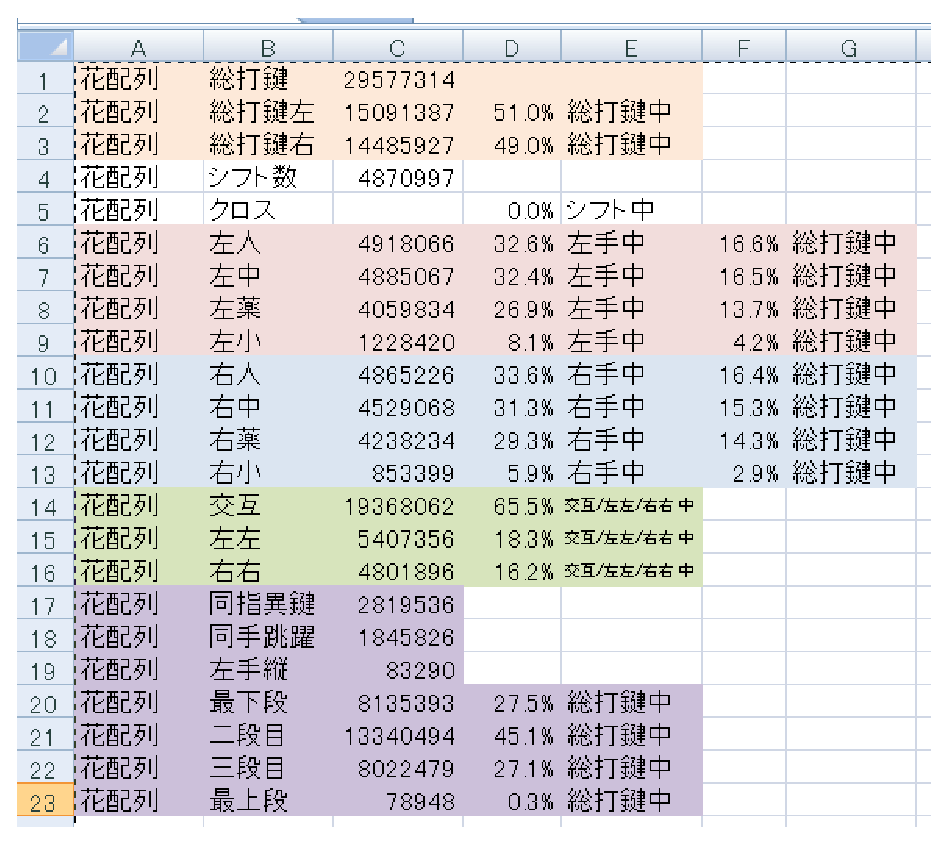
\includegraphics[width=0.85\hsize]{tbl-hana.eps}
% \end{center}
% \caption{�Ԕz��̉�͕\}
% \label{tbl:hana}
%\end{table}

\begin{table*}[htbp]
 \caption{�Ԕz��̉�͕\}
 \begin{center}
 \begin{tabular}{cccc|ccc}
 \hline
���Ō� & ���Ō��� & ���Ō��E & �V�t�g�� & ���� & ���� & �E�E \\
29577314 & 15091387 & 14485927 & 4870997 & 19368062 & 5407356 & 4801896\\
 & 51.0\% & 49.0\% &  & 189.7\% & 53.0\% & 47.0\%\\
 \hline
 \end{tabular}

 �@\vspace{1zw}�@

 \begin{tabular}{ccccccccccc}
 \hline
& ����(A) & ����(S) & ����(D) & ���l(FG) & �E�l(HJ) & �E��(K) & �E��(L) & �E��(;)\\
& 4918066 & 4885067 & 4059834 & 1228420 & 4865226 & 4529068 & 4238234 & 853399\\
��/�E�蒆 & 32.6\% & 32.4\% & 26.9\% & 8.1\% & 33.6\% & 31.3\% & 29.3\% & 5.9\%\\
���Ō��� & 16.6\% & 16.5\% & 13.7\% & 4.2\% & 16.4\% & 15.3\% & 14.3\% & 2.9\%\\
\hline
 \end{tabular}

 �@\vspace{1zw}�@

 \begin{tabular}{ccc|cccc}
 \hline
 ���w�ٌ� & ���蒵�� & ����c & �ʼn��i(ZX..) & �z�[��(AS..) & �O�i��(QW..) & �ŏ�i(12..)\\
2819536 & 1845826 & 83290 & 8135393 & 13340494 & 8022479 & 78948\\
 &  &  & 27.5\% & 45.1\% & 27.1\% & 0.3\%\\
\hline
 \end{tabular}
 \end{center}
 \label{tbl:hana}
\end{table*}

\begin{figure*}[htbp]
 \begin{center}
  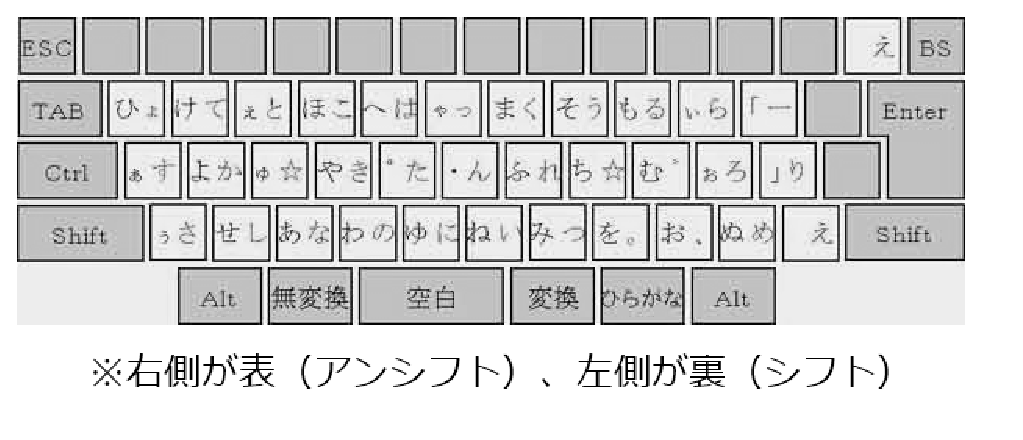
\includegraphics[width=0.8\hsize]{hana.eps}
 \end{center}
 \caption{�Ԕz��}
 \label{fig:hana}
\end{figure*}


�VJIS�Ɠ��l�A���ݑŌ�����6���Ƒ����Ȃ��Ă��܂��B
����A�VJIS�ɔ�ׁi18\%�j�A�ʼn��i��31\%�ƂȂ��Ă���A�����JIS���Ȃ�16\%�Ɣ�r���Ă������g���Ă��܂��B
����ɂ‚��āA�y�~���́u���𕂂����đł‚Ɗy�ɑłĂ�v�Ǝ咣���Ă��܂��B

�������A���蒵��A���w�ٌ��Ȃǂ́A����g�p�����R�[�p�X�ł͐VJIS�̂ق������Ȃ��Ȃ��Ă��܂����B����͎g�p���Ă��镶�͂̕���i�h���C���j�̖����傫������ƍl�����܂��B

\subsubsection*{���z��}

2ch�̐VJIS�X���b�h�łł����J�i�n�z��ŁA�VJIS�ɑ΂��āA�O�q�̉Ԕz��̂悤�Ȓ��w�V�t�g��t��������A�Ƃ����A�C�f�B�A�̂��Ɛ��܂�܂����B
2ch�̃X���b�h�ɂ��邳�܂��܂Ȑl�����ɂ���ĉ��ǂ��d�˂��A�����̔Łi�z��j���ł��܂����B���݂ł�2-263�i�}\ref{fig:tsuki}%
\footnote{�}��\url{http://jisx6004.client.jp/tsuki.html}���B}%
�j�ƌĂ΂�Ă�����̂���ʓI�ł��B

\begin{figure*}[htbp]
 \begin{center}
  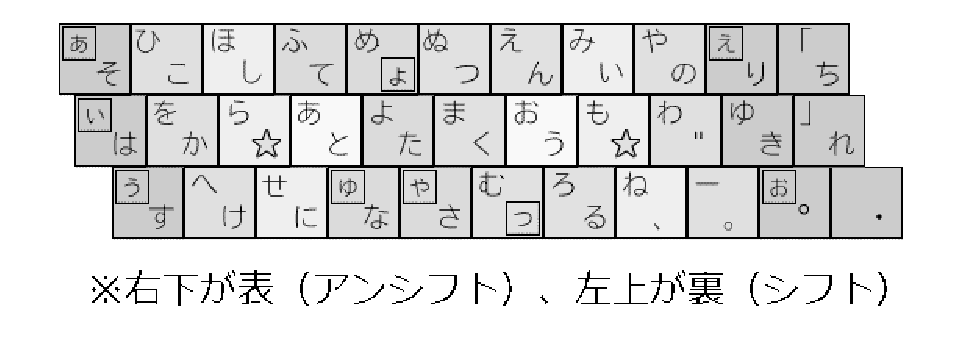
\includegraphics[width=0.8\hsize]{tsuki.eps}
 \end{center}
 \caption{���z��}
 \label{fig:tsuki}
\end{figure*}

�R�[�p�X���g�������̔z��̉�͕͂\\ref{tbl:tsuki}�̂悤�ɂȂ�܂��B

\begin{table*}[htbp]
 \caption{���z��̉�͕\}
 \begin{center}
 \begin{tabular}{cccc|ccc}
 \hline
���Ō� & ���Ō��� & ���Ō��E & �V�t�g�� & ���� & ���� & �E�E \\
29526169 & 14294112 & 15232057 & 4819852 & 19309588 & 4639318 & 5577263\\
 & 48.4\% & 51.6\% &  & 65.4\% & 15.7\% & 18.9\%\\
 \hline
 \end{tabular}

 �@\vspace{1zw}�@

 \begin{tabular}{ccccccccccc}
 \hline
& ����(A) & ����(S) & ����(D) & ���l(FG) & �E�l(HJ) & �E��(K) & �E��(L) & �E��(;)\\
& 5143242 & 5125313 & 2677655 & 1347902 & 4910816 & 5151515 & 4143342 & 1026384\\
��/�E�蒆 & 36.0\% & 35.9\% & 18.7\% & 9.4\% & 32.2\% & 33.8\% & 27.2\% & 6.7\%\\
���Ō��� & 32.2\% & 14.9\% & 19.4\% & 33.5\% & 43.9\% & 32.2\% & 21.5\% & 2.3\%\\
\hline
 \end{tabular}

 �@\vspace{1zw}�@

 \begin{tabular}{ccc|cccc}
 \hline
 ���w�ٌ� & ���蒵�� & ����c & �ʼn��i(ZX..) & �z�[��(AS..) & �O�i��(QW..) & �ŏ�i(12..)\\
2322072 & 996617 & 50003 & 5138841 & 15676342 & 8632038 & 78948\\
 &  &  & 17.4\% & 53.1\% & 29.2\% & 0.3\%\\
\hline
 \end{tabular}
 \end{center}
 \label{tbl:tsuki}
\end{table*}

%\begin{table}[htbp]
% \begin{center}
%  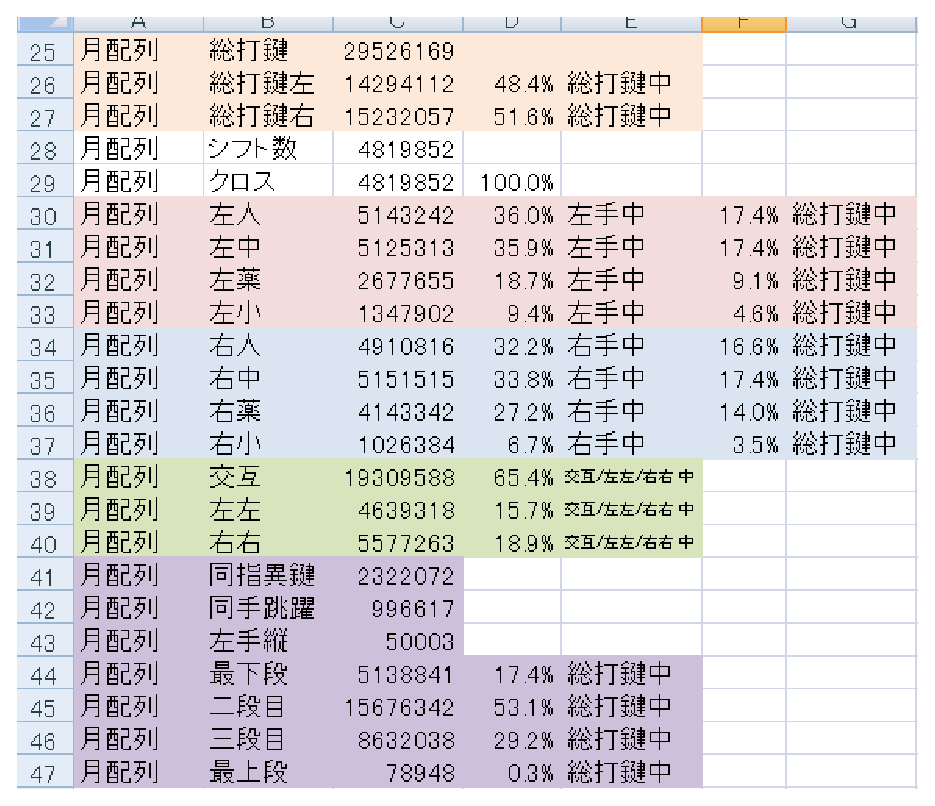
\includegraphics[width=0.85\hsize]{tbl-tsuki.eps}
% \end{center}
% \caption{���z��̉�͕\}
% \label{tbl:tsuki}
%\end{table}

�VJIS�̎����Ă���6���Ƃ������ݑŌ��������̔z����ۂ��Ă��܂��B�VJIS�ɔ�ׁA����/�E�E���o�����X�悭�܂܂�Ă���A��������ϓ��Ɏg�����z��ƌ�����ł��傤�B

\subsection{�e�w�V�t�g�n}
\subsubsection*{NICOLA}

OASYS�z��A�܂���NICOLA�z��́u�e�w�V�t�g�z��v�ƌĂ΂�A
�L�[�{�[�h�̃X�y�[�X�L�[�ɂ�����Ƃ���ɁA�}\ref{fig:nicola}�̂悤�ȓ�‚́u�e�w�V�t�g�L�[�v�������Ă���̂������ł��B

�}8�̃L�[�ɂ͎O�‰����������Ă���܂��ˁB
���ɂ��镶���͂��̂܂ܑł��A��ɂ��镶���́u���̕����Ɠ�����ŃV�t�g�������Ȃ���v�i����V�t�g�j�ł��܂��B
�����ɂ‚��ẮA�u�����̃L�[�Ɣ��Α��̎�ŃV�t�g�������Ȃ���v�i�N���X�V�t�g�j�ł��܂��B
���̎d�l�̂��߁A�e�w�V�t�g�ł́A�����i�������t�������j�͂��ׂĒP�ƂőłĂ镶���ƂȂ��Ă��܂��B

\begin{figure*}[htbp]
 \begin{center}
  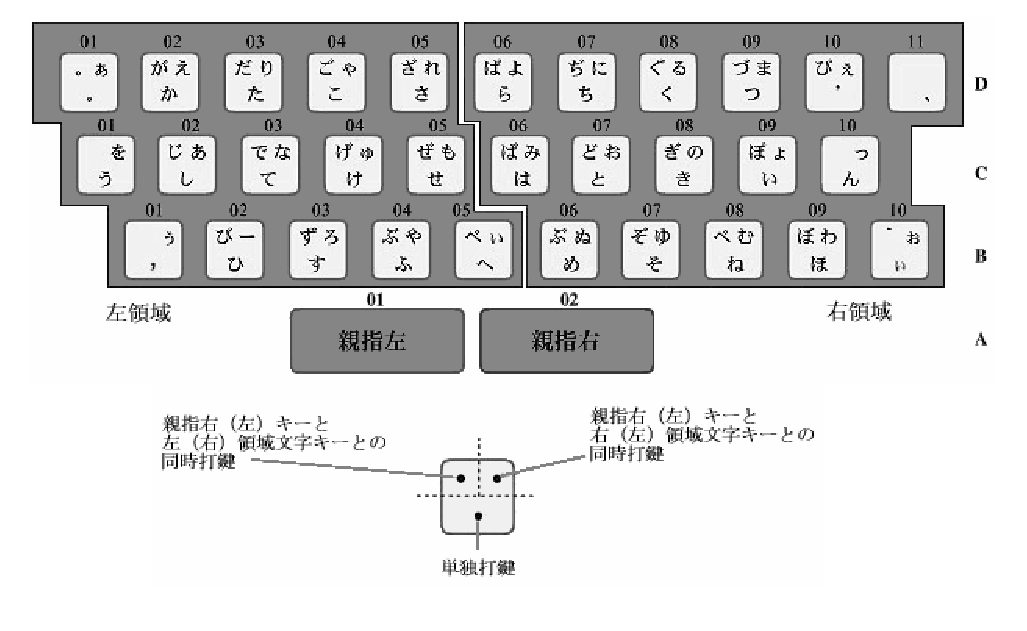
\includegraphics[width=0.8\hsize]{nicola.eps}
 \end{center}
 \caption{NICOLA�z��i�}��NICOLA�z��K�i�����j}
 \label{fig:nicola}
\end{figure*}

�e�w�V�t�g�z��̋N���́A1980�N�A�x�m�ʂ�OASYS100�Ƃ������[�v����p�@�Ɏn�܂�܂��B
����ȍ~�A��т���OASYS�͐e�w�V�t�g���̗p���A�����̎x���҂𐶂�ł��܂����B
���{��ɓK�������͕����̕��y�ƕW������ړI�Ƃ��āA1989�N�ɔ��������ƊE�c�́u���{����̓R���\�[�V�A���v�́A
�x�m�ʂ̐e�w�V�t�g�L�[�{�[�h�����ǂ��A�uNICOLA�z��v��񏥂��܂����B

��̓I�ȑ���_�Ƃ��ẮAOASYS�ł͔��������u�������L�[�v��p���ĉ����Ă����̂ɑ΂��A
NICOLA�ł͐e�w�ʼn�����悤�ɂ��܂����B
�܂��A�ŏ�i�̋L����A�o�b�N�X�y�[�X�A���s�L�[�Ȃǂ̈ʒu��NICOLA�ł�JIS�K�i�̃L�[�{�[�h�ɍ��킹�Ă��܂��B

�u�L�[�{�[�h���Ȋw����v\footnote{\url{http://www.fmworld.net/oasysworld/cat/dgt01.html}}%
�ɂ��ƁA
\begin{itemize}
\item �u�l�����w�������΂�g���₷���A���w�������΂�g���ɂ����v
\item �u�w�̎g���₷���́A���i�i�z�[���|�W�V�����j�A��i�A���i�̏��v
\item �u�����w�A�ׂ荇�����w�̎g�p�͔�����v
\item �u�������̎�ł͂Ȃ��A���E���݂Ɏg�������ł��₷���v
\end{itemize}
�܂��A�i�_�c��, 1979�j�ɂ���
\begin{itemize}
\item �u�����̏o���p�x����јA�ڏo���p�x�v�iunigram��bigram�j���l��
\end{itemize}
�Ƃ����݌v�v�z�Ɋ�Â��ăf�U�C������܂����B

�_�c��́i����OASYS�̐e�w�V�t�g�z��́j�]���Ƃ��āA6�l�Ɉ��0.5�`1.5���Ԃ̗��K���ꃖ���s�킹�܂����B���̎����ɂ��A
\begin{itemize}
\item �����L�[�͊��S�Ƀ^�b�`�^�C�s���O�ł���
\item �����L�[�Ɛe�w�V�t�g�L�[�𓯎��ɉ����̂́A�L�[��P�Ƃőł‚̂Ɠ������o�ōs����
\end{itemize}
���Ƃ��킩��A����ɑŌ����x�Ƃ���80�`180��/��������ꂽ�Ƃ������Ƃł��B

����ł̓R�[�p�X���g���Ă݂Ă݂܂��傤�i�\\ref{tbl:nicola}�j�B�����ł͑����̐e�w�V�t�g�G�~�����[�^�ō̗p����Ă���NICOLA�z���]�����邱�Ƃɂ��܂��B

\begin{table*}[htbp]
 \caption{NICOLA�̉�͕\}
 \begin{center}
 \begin{tabular}{cccc|ccc}
 \hline
���Ō� & ���Ō��� & ���Ō��E & �V�t�g�� & ���� & ���� & �E�E \\
 22009710 & 11180976 & 10828734 & 9331864(2892628) & 11729133 & 5316409 & 4964168\\
 & 50.8\% & 49.2\% &  & 53.3\% & 24.2\% & 22.6\%\\
 \hline
 \end{tabular}

 �@\vspace{1zw}�@

 \begin{tabular}{ccccccccccc}
 \hline
& ����(A) & ����(S) & ����(D) & ���l(FG) & �E�l(HJ) & �E��(K) & �E��(L) & �E��(;)\\
& 2817456 & 3264915 & 3278771 & 1819834 & 3709821 & 2606899 & 2770957 & 1741057\\
��/�E�蒆 & 25.2\% & 29.2\% & 29.3\% & 16.3\% & 34.3\% & 24.1\% & 25.6\% & 16.1\%\\
���Ō��� & 12.8\% & 14.8\% & 14.9\% & 8.3\% & 16.9\% & 11.8\% & 12.6\% & 7.9\%\\
\hline
 \end{tabular}

 �@\vspace{1zw}�@

 \begin{tabular}{ccc|cccc}
 \hline
 ���w�ٌ� & ���蒵�� & ����c & �ʼn��i(ZX..) & �z�[��(AS..) & �O�i��(QW..) & �ŏ�i(12..)\\
1834583 & 1036799 & 118061 & 2619704 & 11735857 & 7575201 & 78948\\
 &  &  & 11.9\% & 53.3\% & 34.4\% & 0.4\%\\
\hline
 \end{tabular}
 \end{center}
 \label{tbl:nicola}
\end{table*}



%\begin{table}[htbp]
% \begin{center}
%  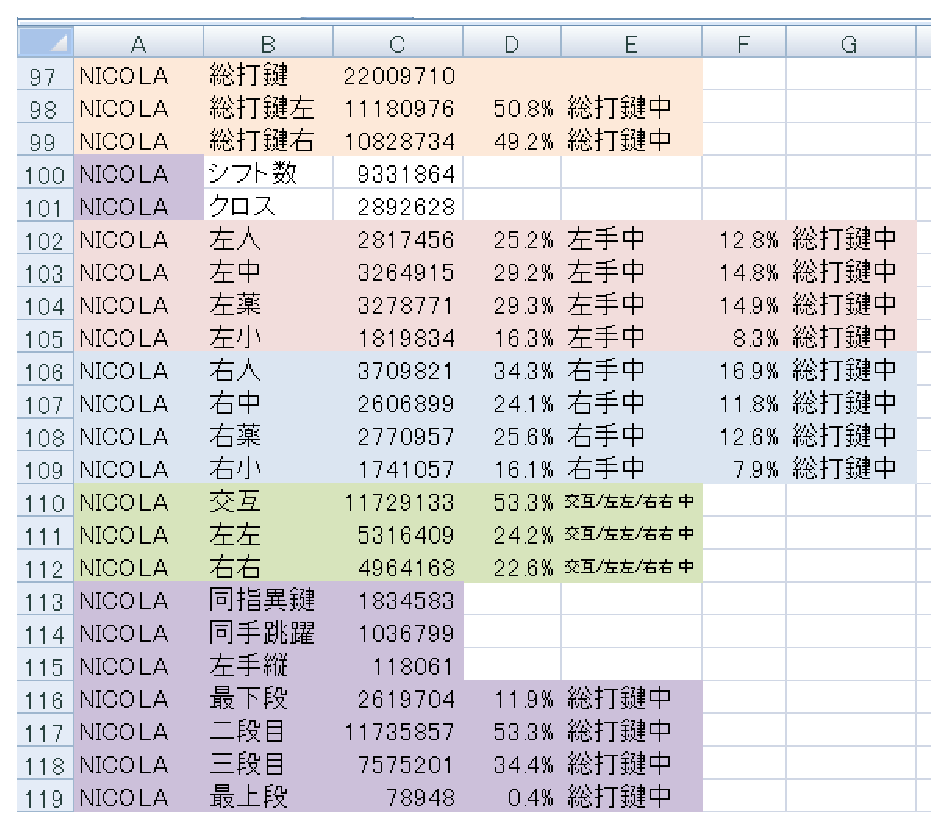
\includegraphics[width=0.85\hsize]{tbl-nicola.eps}
% \end{center}
% \caption{NICOLA�z��̉�͕\}
% \label{tbl:nicola}
%\end{table}

NICOLA�ł͂��̐݌v�v�z�ʂ�A���E�o�����X�悭�A�܂��A�قǂ悭���ݑŌ��������悤�ɔz�񂳂�Ă��܂��B
�܂��A�z�[���|�W�V�����̎g�p����54\%�ƁA�Ȃ�ׂ��w���痣��Ȃ��悤�ɂȂ��Ă��܂��B
���Ō���43\%��4�����V�t�g�Ȃ̂͋C�ɂȂ�Ƃ���ł����A���[�U�e�X�g�ɂ��΋C�ɂȂ�Ȃ��悤�ł��̂ŁA
�悵�Ƃ��܂��傤�B

�Ȃ��A�V�t�g���������̂́u�́v�u�ȁv�u��v�Ȃǂ̍��p�x�̕������V�t�g�ɔz�񂳂�Ă��邽�߂ƍl�����܂��B�����L�[���V�t�g�Ɋ��蓖�Ă˂΂Ȃ�Ȃ������h���ł��傤�B
�Q�l�̂��߁A�����o�����20�‚̂����A���i�V�t�g���j�ɂȂ��Ă��܂��������������܂�\footnote{�u��v�Ƃ‚���ƌ��Â炢�̂ŁA�ȗ����܂����B���ׂėL��������2���ł��B}�F�u�́v�i5��; 4.0\%�j�A�u�Ɂv�i9��; 2.8\%�j�A�u�ȁv�i11��; 2.5\%�j�A�u��v�i15��; 2.2\%�j�A�u���v�i18��; 2.0\%�j�܂��A�t�ɒ�p�x�Ȃ̂ɕ\�ɗ�����𓾂Ȃ����������̉����������܂��傤�B�u�ցv�i0.23\%�j�A�u�فv�i0.48\%�j�A�u�Ӂv�i0.48\%�j�A�u�Ёv�i0.61\%�j�ȂǂȂǁB

%\subsubsection*{TRON�z��}
\subsubsection*{�򒹔z��}

Ray���ɂ���čl�Ă��ꂽ�e�w�V�t�g�z��ł���򒹔z��́A���ǂɉ��ǂ��d�˂č���܂����B���̐݌v�v�z��
\begin{itemize}
\item �E����悭�g��\footnote{�������̐l�p�Ɂu���t�e�B�򒹁v�Ƃ������̂��p�ӂ���Ă��܂��B}
\item �e�w�L�[���������ςȂ��ɂ�����Ԃł̘A�����́i���̃L�[��A���œ��͂���j���Ƃ�ϋɓI�Ɏ�����Ă���icf. NICOLA�ł͈�Ō����ƂɈ�V�t�g�j
\end{itemize}

�򒹔z��͂��̗��j�����ʂɔł�����܂�%
\footnote{����p�����̂́A�򒹔z��383�ł̂����A�����̔z��123\ldots �ƂȂ��Ă���u�򒹔z��123-383�Łv�ł��B}
���A���̈���}\ref{fig:asuka}�Ɏ����܂�%
\footnote{�}��\url{http://ameblo.jp/asuka-layout/entry-10334710008.html}���B}%
�B�u�����������v�Ȃǂ̑�������‚̃L�[�œ��͂���̂������ł��B

\begin{figure*}[htbp]
 \begin{center}
  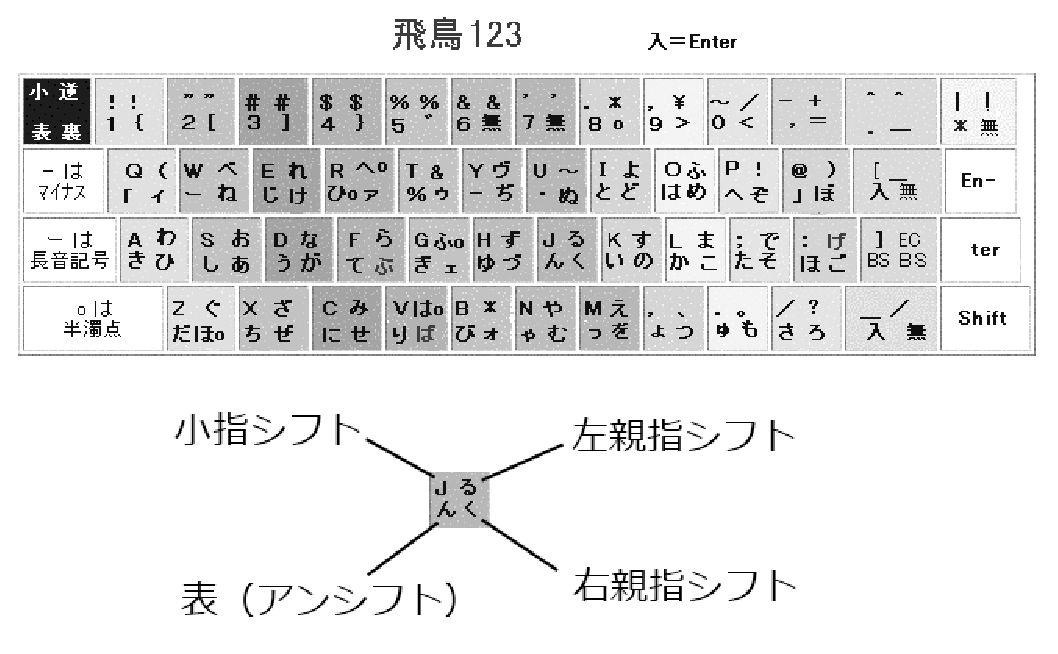
\includegraphics[width=0.8\hsize]{asuka.eps}
 \end{center}
 \caption{�򒹔z��123-383��}
 
 \label{fig:asuka}
\end{figure*}

����ł̓R�[�p�X���g���ĕ]�����Ă݂܂��B
%�i����̕]���v���O�����ł́A�u�V�t�g���������ςȂ��̘A�����́v���ʓI�ɗʂ邱�ƂɑΉ����Ă��܂���ł����B����ȍ~�̉ۑ�Ƃ��܂��j�B

\begin{table*}[htbp]
 \caption{�򒹔z��̉�͕\}
 \begin{center}
 \begin{tabular}{cccc|ccc}
 \hline
���Ō� & ���Ō��� & ���Ō��E & �V�t�g�� & ���� & ���� & �E�E \\
22329794 & 8913749 & 13416045 & 10594571(5240353) & 11489323 & 3169088 & 7671383\\
 & 39.9\% & 60.1\% &  & 65.5\% & 18.1\% & 43.8\%\\
 \hline
 \end{tabular}

 �@\vspace{1zw}�@

 \begin{tabular}{ccccccccccc}
 \hline
& ����(A) & ����(S) & ����(D) & ���l(FG) & �E�l(HJ) & �E��(K) & �E��(L) & �E��(;)\\
1575536 & 3914260 & 2128521 & 1295432 & 3437742 & 4878650 & 3246516 & 1853137\\
��/�E�蒆 &17.7\% & 43.9\% & 23.9\% & 14.5\% & 25.6\% & 36.4\% & 24.2\% & 13.8\%\\
���Ō��� & 7.1\% & 17.5\% & 9.5\% & 5.8\% & 15.4\% & 21.8\% & 14.5\% & 8.3\%\\
\hline
 \end{tabular}

 �@\vspace{1zw}�@

 \begin{tabular}{ccc|cccc}
 \hline
 ���w�ٌ� & ���蒵�� & ����c & �ʼn��i(ZX..) & �z�[��(AS..) & �O�i��(QW..) & �ŏ�i(12..)\\
1988288 & 930019 & 20753 & 6033749 & 12828047 & 3389059 & 78939\\
 &  &  & 27.0\% & 57.4\% & 15.2\% & 0.4\%\\
\hline
 \end{tabular}
 \end{center}
 \label{tbl:asuka}
\end{table*}

%\begin{table}[htbp]
% \begin{center}
%  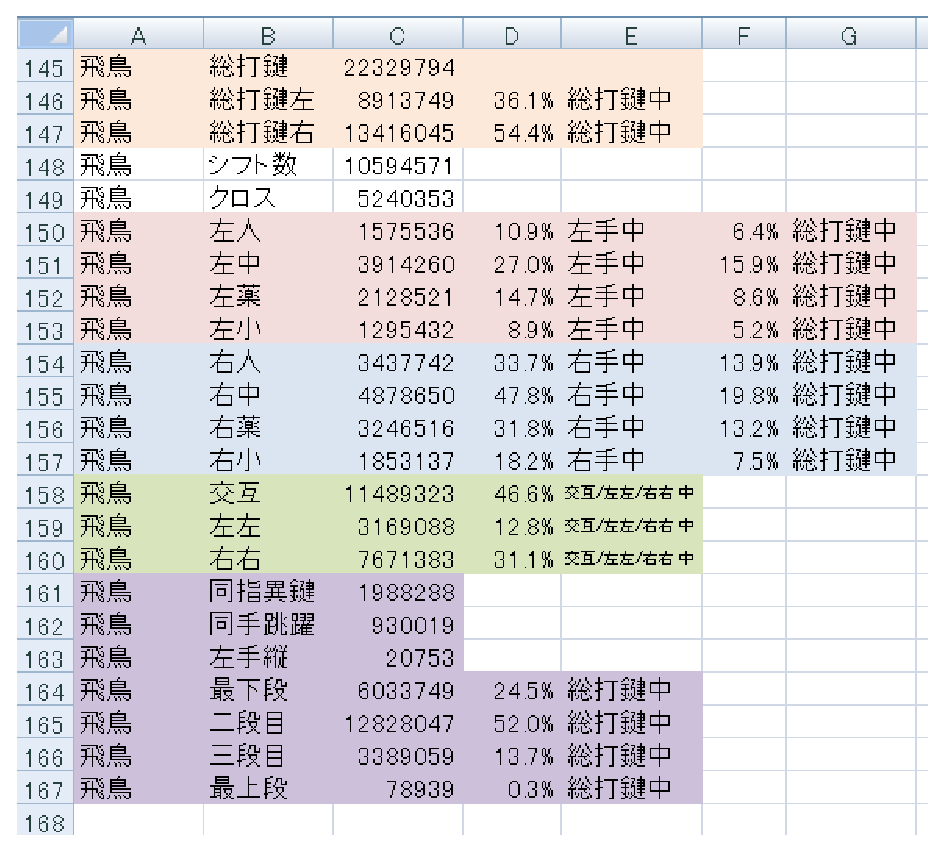
\includegraphics[width=0.85\hsize]{tbl-asuka.eps}
% \end{center}
% \caption{�򒹔z��i383�Łj�̉�͕\}
% \label{tbl:asuka}
%\end{table}

�݌v�v�z�ʂ�A�E��̎g�p������54\%�ƍ����Ȃ��Ă��܂��B�܂��A���ݑŌ�������47\%�A�����ĉE���E�̓��͂���31\%�ƁA���ݑŌ������‚A���ӂȉE����g���Ă�����Ƃ����A�o�����X�̂Ƃꂽ�z��ɂȂ��Ă��܂��B

���M���ׂ��͍���c�A�̏��Ȃ��ł��BNICOLA�̂���Ɣ�ׂĂ�17\%�Ƃ������Ȃ��ł��i��: 20753�ANICOLA: 118061�j�B
�򒹔z��̓V�t�g���������܂܂̘A�����͂ɂ����܂ł�������������ʁA�A���y�W�I�^�w�𑽂����ݏo�����̂ł��傤���i����g�p������̓X�N���v�g�ł́A�A���y�W�I�^�w�͍l�����Ă��܂���ł����B����ȍ~�̉ۑ�Ƃ��܂��j�B

�܂��A�ʼn��i�̎g�p��NICOLA�ɔ�ׂđ����A�Ԕz��Ɠ��l�A�i�p�[�����X�g�Ȃǂ��g���āj��𕂂����ē��͂���̂Ɍ����Ă���ƍl�����܂��B

\subsection*{���~�z��}

���~�z���NICOLA�ATRON�z��A�򒹔z��̗�������ސe�w�V�t�g�z��ŁA�N���X�V�t�g�ő�������͂�������������Ă��܂��i�}\ref{fig:koume}%
\footnote{�}��\url{http://homepage2.nifty.com/61degc/reports/koume/} ���B}�j�B

�݌v�v�z�Ƃ��āANICOLA�Ɠ��l�ɃN���X�V�t�g�ő�������͂��A�L���ɑ΂��镉�ׂ����炵�Ă��܂��B�A���V�t�g�ł͂Ȃ��A���̓s�x�V�t�g����͂�����_��NICOLA�Ɠ��l�ł��B
�܂��A���ݑŌ����������������ŁA�����̐l�̗�����ł���E��̎g�p�p�x���������Ă��܂��B��̓I�ɂ́A���E�̎g�p�p�x������F�E�聁43�F57�Ɛݒ肵�Ă��܂��i��q����悤�ɁA����̓R�[�p�X�ł��m�F�ł��܂��j�B

\begin{figure*}[htbp]
 \begin{center}
  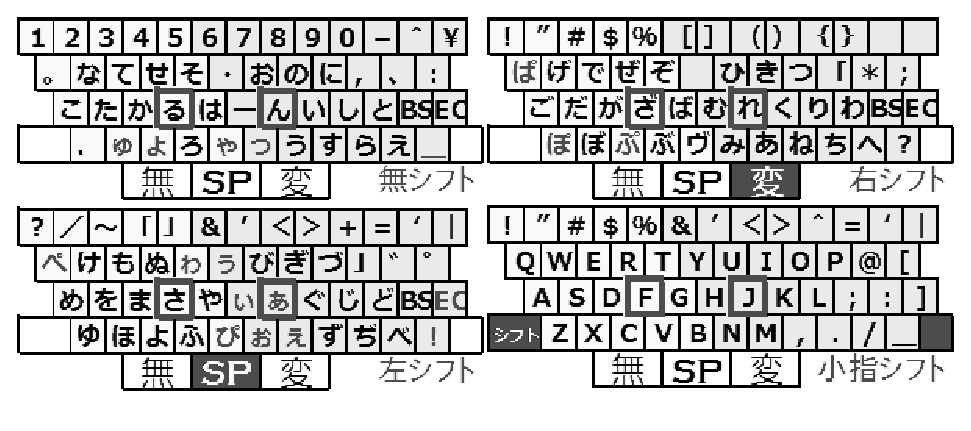
\includegraphics[width=0.8\hsize]{koume.eps}
 \end{center}
 \caption{���~�z��}
 \label{fig:koume}
\end{figure*}

����ł̓R�[�p�X���g���ĕ]�����Ă݂܂��B%�i����̕]���v���O�����ł́A�u�V�t�g���������ςȂ��̘A�����́v���ʓI�ɗʂ邱�ƂɑΉ����Ă��܂���ł����B����ȍ~�̉ۑ�Ƃ��܂��B�j
����F�E��̎g�p�p�x����44:56�ƁA�݌v�v�z�ʂ�ɂȂ��Ă��邱�Ƃ����������܂��B�܂��A���ݑŌ����E�E��g�p���i�E���E�j���Ƃ��ɍ����Ȃ��Ă��܂��B

\begin{table*}[htbp]
 \caption{���~�z��̉�͕\}
 \begin{center}
 \begin{tabular}{cccc|ccc}
 \hline
���Ō� & ���Ō��� & ���Ō��E & �V�t�g�� & ���� & ���� & �E�E \\
 22366745 & 9793272 & 12573473 & 8115349(2609182) & 12832519 & 3377012 & 6157214\\
 & 43.8\% & 56.2\% &  & 57.4\% & 15.1\% & 27.5\%\\
 \hline
 \end{tabular}

 �@\vspace{1zw}�@

 \begin{tabular}{ccccccccccc}
 \hline
& ����(A) & ����(S) & ����(D) & ���l(FG) & �E�l(HJ) & �E��(K) & �E��(L) & �E��(;)\\
& 2620589 & 3462294 & 2461322 & 1249067 & 4025676 & 3719075 & 3191966 & 1636756\\
��/�E�蒆 & 26.8\% & 35.4\% & 25.1\% & 12.8\% & 32.0\% & 29.6\% & 25.4\% & 13.0\%\\
���Ō��� & 11.7\% & 15.5\% & 11.0\% & 5.6\% & 18.0\% & 16.6\% & 14.3\% & 7.3\%\\
\hline
 \end{tabular}

 �@\vspace{1zw}�@

 \begin{tabular}{ccc|cccc}
 \hline
 ���w�ٌ� & ���蒵�� & ����c & �ʼn��i(ZX..) & �z�[��(AS..) & �O�i��(QW..) & �ŏ�i(12..)\\
1962705 & 1135597 & 18698 & 4734636 & 10838801 & 6627420 & 165888\\
 &  &  & 21.2\% & 48.5\% & 29.6\% & 0.7\%\\
 &  &  & ���Ō��� & ���Ō��� & ���Ō��� & ���Ō���\\
\hline
 \end{tabular}
 \end{center}
 \label{tbl:roma}
\end{table*}

%\begin{table}[htbp]
% \begin{center}
%  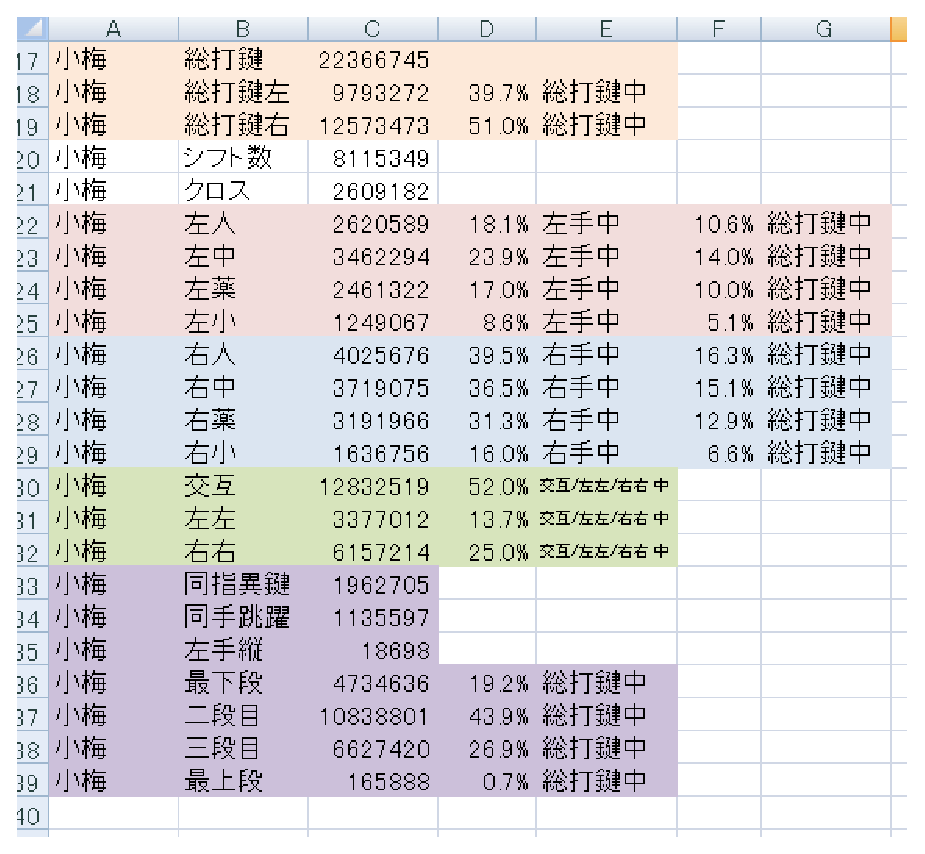
\includegraphics[width=0.85\hsize]{tbl-koume.eps}
% \end{center}
% \caption{���~�z��̉�͕\}
% \label{tbl:koume}
%\end{table}

\subsection{��`�I�A���S���Y���ɂ��z�񌈒�}

�O�q�̉Ԕz��̂����炢�����܂��傤�B�Ԕz��ł́A�u�悢�z��v���܂���`���A�����_���Ȕz�u���珉�߂āA�g�ݍ��킹���������u�悢�����ցv�ς��Ă������̂ł����B
���̂悤�ɁA�u�悳�v�i{\bf �]���l}�j���`���āA�]���l�̂ł��邾�������i�ő�ƂȂ�̂��]�܂����j�������߂�����u�T�����v�ƌ����܂��B
���ɁA�����z��̂悤�ȑg�ݍ��킹�̏ꍇ�A�u{\bf �g�ݍ��킹�œK�����}�v�ƌĂт܂��B

��ʂɁA�g�ݍ��킹�œK�����͑g�ݍ��킹�̐����c��ɂȂ��Ă��܂����߁A�T��������ł��B���Ƃ��΁A�����̕���55�‚ƋL��8�‚̌v63�‚�P���ɕ��ׂ���ו���$63!$�ʂ�ł��B
�����$10^{87}$����$2^{289}$�����傫�����ŁA���̑g�ݍ��킹�����ׂĒT���i�S��T���A���邢�͑S�T���Ƃ����܂��j����̂͌����I�ł͂���܂���B

�����ŁA�S�T�������Ȃ��łł��邾���悢�������߂�A���S���Y���������‚����݂��܂��B�������������̂́A�����̈�`�q��͂����u��`�I�A���S���Y���v�Ƃ������̂ł��B
{\bf ��`�I�A���S���Y��}�́A���̌����u��`�q�v�Ƃ����`�ŕ\�����A�������u�������킹�v�i\ruby{{\bf ����}}{������}�j�ĐV�����‘́i���j�𐶐����A
����ɕ]���l�ɂ���āu�ꕔ�̂ݐ����c�点��v�i�����R\ruby{����}{�Ƃ���}; {\bf �I��}�j���Ƃ��J��Ԃ����Ƃɂ���āA���悢����T�����܂��B
�܂��A�����̍ۂɉ��̈ꕔ��ω�������i�ˑR{\bf �ψ�}�j���Ƃ����܂��B
���̂悤�ɁA�����̐i����͂��Ă��邽�߁A�i���I�A���S���Y���̈��Ƃ���܂��B

�������A���鉼���z��Ɖ����z���P���ɂ������킹��i������j�����ł́A�����L�[����J���o�Ă�����A���݂��Ȃ��L�[���o�Ă�����ƁA�g�����̂ɂȂ�Ȃ��z�񂪂ł��Ă��܂��܂��B
���̂悤�Ȕz��i��`�q�j���u{\bf �v����`�q}�v�ƌ����܂��B
�v����`�q�𔭐������Ȃ��������ǂ��������邩�A���邢�͂���������`�q���ǂ��\�����邩�́A�ƂĂ�������ł��B

�܂��A�]���l�̌v�Z���d�v�ł��B��`�I�A���S���Y���ł́A�P��̕]���l��p���Đ����c���`�q�����߂Ă��܂����B
�K�؂ȕ]�����p���Ȃ��ƁA�ӂ��킵���Ȃ���`�q�������c���Ă��܂����ƂɂȂ�A��͂�悢���͓����܂���B

���̂悤�Ɏg���ǂ��낪�����`�I�A���S���Y���ł����A
��ʂɑS�T��������Ȗ��ɑ΂��Ă���Ȃ�ɗǂ��������߂���Ƃ������ƂŁA
�ꎞ���A�ꐢ��\ruby{���r}{�ӂ���}�����Ƃ����ߋ��������܂��B

\subsubsection*{��s�����i�����z��ȊO�j}

��`�I�A���S���Y���ɂ��L�[�{�[�h�z��݌v�ł́A�k�C���h�Řb����Ă���q���f�B�[���
�L�[�{�[�h�̐݌v [Deshwal and Kalyanmoy, 2003]��A�A���t�@�x�b�g�̃\�t�g�E�F�A�L�[�{�[�h�̐݌v [Raynal and Vigouroux, 2005] �Ȃǂōs���Ă��܂��B

Deshwal��̐݌v�ł́A��‚̈�`�q�i�z��j$G_1$��$G_2$���������Ƃ��A�܂�$G_1$�̔������c���A
�c��̔����̃L�[��$G_2$�̃L�[�́u�߂��v�ɕ��בւ���i��$G_2$�̃L�[���Q�l�ɂ��ĉ��ǂ���j
���ƂŁA�v����`�q����邱�ƂȂ��������������Ă��܂��B
�܂��A�]���֐��Ƃ��āA���ݑŌ����𑝂₷�A�����w�ŃL�[��ł��Ȃ��A�Ȃǂ�p���Ă��܂��B

Raynal��́A�O��m���҂ŏЉ���t�B�b�c�̖@����p���Ă��܂��B�\�t�g�E�F�A�L�[�{�[�h�ł̓}�E�X��y�����g���̂ŁA�t�B�b�c�̖@�����N���e�B�J���Ɍ����Ă���̂ł��傤�B

\subsubsection*{�K�Ԕz��i����:���z��j}

��`�I�A���S���Y���𒆎w�V�t�g�����z��̐݌v�ɗp�����̂��A�K�Ԕz��i����:���z��j�ł�%
\footnote{\url{http://www.geocities.jp/rage2050a/GeneKana/_ReadMe.html}}%
�i�}\ref{fig:maru}�j�B

\begin{figure*}[htbp]
 \begin{center}
  \includegraphics[width=0.8\hsize]{maru.eps}
 \end{center}
 \caption{���z��}
 \label{fig:maru}
\end{figure*}

�����́A�����_���ɃL�[�̈ʒu��I�сA�����_���ɔz��i��`�q�j$G_1$�A$G_2$�̂ǂ��炩��I��ł����A
���ׂẴL�[�ɉ�����u���܂ŌJ��Ԃ��A�Ƃ������̂ł��B
�������N����i�������������łɒu����Ă���j�ꍇ�ɂ́A
�L�[�z��̍��ォ�珇�ɂ܂��u����Ă��Ȃ����̂�I�ԁA�Ƃ������@�ʼn������Ă��܂��B
�]���ɂ͊J���҂����g�ŃL�[��bigram�ɂ‚��đŌ����Ԃ��v�����A���̑g�ݍ��킹��p���܂����B

����ł̓R�[�p�X���g���ĕ]�����Ă݂܂��傤�i�\\ref{tbl:maru}�j�B

\begin{table*}[htbp]
 \caption{���z��̉�͕\}
 \begin{center}
 \begin{tabular}{cccc|ccc}
 \hline
���Ō� & ���Ō��� & ���Ō��E & �V�t�g�� & ���� & ���� & �E�E \\
29756111 & 14149812 & 15606299 & 5049787 & 19866174 & 4216725 & 5673212\\
 & 47.6\% & 52.4\% &  & 66.8\% & 14.2\% & 19.1\%\\
 \hline
 \end{tabular}

 �@\vspace{1zw}�@

 \begin{tabular}{ccccccccccc}
 \hline
& ����(A) & ����(S) & ����(D) & ���l(FG) & �E�l(HJ) & �E��(K) & �E��(L) & �E��(;)\\
& 5020769 & 4841928 & 2420872 & 1866243 & 4788744 & 4902439 & 4506402 & 1408714\\
��/�E�蒆 &35.5\% & 34.2\% & 17.1\% & 13.2\% & 30.7\% & 31.4\% & 28.9\% & 9.0\%\\
���Ō��� & 16.9\% & 16.3\% & 8.1\% & 6.3\% & 16.1\% & 16.5\% & 15.1\% & 4.7\%\\
\hline
 \end{tabular}

 �@\vspace{1zw}�@

 \begin{tabular}{ccc|cccc}
 \hline
 ���w�ٌ� & ���蒵�� & ����c & �ʼn��i(ZX..) & �z�[��(AS..) & �O�i��(QW..) & �ŏ�i(12..)\\
2003058 & 1082831 & 47820 & 5960127 & 16389169 & 7327867 & 78948\\
 &  &  & 20.0\% & 55.1\% & 24.6\% & 0.3\%\\
\hline
 \end{tabular}
 \end{center}
 \label{tbl:maru}
\end{table*}

%\begin{table}[htbp]
% \begin{center}
%  \includegraphics[width=0.85\hsize]{tbl-maru.eps}
% \end{center}
% \caption{���z��̉�͕\}
% \label{tbl:maru}
%\end{table}

���ݑŌ�������67\%�ƁA�ԁA���z����኱���鍂���ł��B
�]���l�ɂ͎����̑Ō����Ԃ��p�����Ă���̂ŁA���ݑŌ��̑����������ł��܂��B

�z�[���|�W�V�����̑Ō�������55\%�ƁA���A�Ԃ��������Ȃ��Ă��܂��B
����c�A�̏��Ȃ��i�K��:47820�A��:83290�A��:50003�j�����͓I�ł��B

\subsection{�܂Ƃ�}

�Ō�ɁA���܂ŏo�Ă����z����܂Ƃ߂Ĕ�r���Ă݂܂��傤�i�\\ref{tbl:matome}�ƕ\\ref{tbl:matome-percent}�j�B
�Ȃ��A�\\ref{tbl:matome-percent}�̃p�[�Z���g�\�L�́A
\begin{itemize}
 \item ���Ō����E�E�͑��Ō����̊���
 \item �V�t�g�E�N���X�V�t�g�͑��Ō����̊���
 \item ��\{���򒆐l\}�E�E\{�l����\}�͑��Ō����ɐ�߂銄��
 \item (1)���݁E(2)�����E(3)�E�E�́A���̎O�‚̊����B�‚܂� $ \frac{(1)}{\left\{(1)+(2)+(3)\right\}} $ �Ȃǂ̊����B
 \item �ʼn��i�`�ŏ�i�͂��ꂼ��̑S�Ō��ɐ�߂銄���i�����Ō��ɂ����銄���j
\end{itemize}
�ł��B

AZIK�̃^�C�v���̍팸���́A���w�V�t�g�z��ɔ��鐨���ł��B�C�ɂȂ�͍̂��菬�w�̎g�p���̍����ł����A����͂�����\key{Q}�Ɓi�O�ɉE��̃L�[�������Ƃ���-an�ł���j\key{Z}�ɂ����̂ł��B���ۂ̉^�w�ł́A���Ɂu����v�i\key{K}\key{N}�j�Ȃǂ͉E�����őł‚��Ƃ����邽�߁A��⋭���ȉ��肾������������܂���B

���ݑŌ��ɂ‚��Ă͍���A�u���w�V�t�g�͂��ׂăN���X�V�t�g�v�Ƃ�����������������߁A��/��/�K�ԁi���j�z��ɗL���ɂȂ��Ă��܂��B
���ۂ̉^�w�ɂ���Ă̓A���y�W�I�^�w�ɂȂ邱�Ƃ��\�����肦�܂��̂ŁA���ʂ�����Ƃ��͂����ӊ肢�܂��B

���ݑŌ������ɂ������VJIS�ANICOLA�A���~�ɔ�ׂāA�򒹔z��̌��ݑŌ��������Ⴍ�Ȃ��Ă���̂����ĂƂ�܂��B
�򒹔z��ł͂��̑���A�E�E�̔䗦�������Ȃ��Ă���A�A���y�W�I�^�w��_���Ă��邱�Ƃ���������܂��B%
%�i�������A����̉�̓v���O�����ł́A�A���y�W�I�ɂ‚��Ă͒��ׂ邱�Ƃ��ł��܂���ł����j�B

�l�����w�͓���S�����邽�߁A��ʓI�Ɏg�p�䗦�������Ȃ肪���ł��B���ہA�����̔z��Łu���l/�E�l�v�̒l�͍����Ȃ��Ă��܂��B
����A�򒹔z��ɂ‚��Ă͐l�����w�̎g�p�����Ⴍ�Ȃ��Ă��邱�Ƃɒ��ڂ��܂��傤�B����͔򒹔z��̐݌v�v�z�̈�A�u�l�����w�̂����A\key{T}��\key{Y}�̂����͉����̂Ŕ�����v�𔽉f���Ă�����̂ƌ����܂��傤�B

\subsection{���Ƃ���}

�����QWERTY�A����щ����z��ɏœ_�𓖂ĂĂ��܂����B
���̂��߁ADvorak��AAZIK��Dvorak�łł���ACT�ɐG��邱�Ƃ��ł��܂���ł����B
�܂��A�򒹔z��ɂ�����A���V�t�g�i�A���y�W�I�^�w�j�ɂ‚��Ă̌������ł��܂���ł����B

��s�����ɂ����āA�u�i�e�w�́j�V�t�g����̓^�C�s���O�ɉe�����y�ڂ��Ȃ��v�Ƃ������Ƃ͂����A
�M�҂̎����ł̓V�t�g����͂��Ǝw�i�Ɠ��j�ɕ��S���������Ă���悤�Ȉ�ۂ��󂯂܂��B

����A�܂����̂悤�ȕ��͂������@�����΁A�����ƍׂ��������܂ŋÂ炵���l�@���ڂ������ƍl���Ă��܂��B
�܂��A�����̖ړI�ł������u�ł��₷���v�L�[�{�[�h�z������߂āA�z��݌v�ɂ‚��Ă����͂�\ruby{�F}{������}�߂���
�ł��B���ɕM�҂�AZIK�ɑ傫�ȉ”\�������������Ă��邽�߁A���񏑂����悤�Ȓm�����������AAZIK�̍œK�z�u��
�v�Z�ɂ���ċ��߂����Ǝv���Ă��܂��B�ł́A�܂��ǂ����ŁB

\clearpage

\begin{table*}[htbp]
 \caption{�܂Ƃ߁i�l��1000�Ŋ����Ă���j}
 \begin{center}
  \includegraphics[angle=90, width=0.85\hsize]{matome-table.eps}
 \end{center}
 \label{tbl:matome}
\end{table*}

\clearpage

\begin{table*}[htbp]
 \caption{�܂Ƃ߁i�p�[�Z���g�\�L�j}
 \begin{center}
  \includegraphics[angle=90, width=0.85\hsize]{matome-table-percent.eps}
 \end{center}
 \label{tbl:matome-percent}
\end{table*}



\clearpage
\articlepart{�^�C�s���O�ƃL�[�{�[�h}{eigh8\_t}

\section{�͂��߂�}
�^�C�p�[�ɂƂ��ăL�[�{�[�h�ƌ�������ǂ�ȑ��݂ł��傤���B�L�[�{�[�h�̓^�C�s���O�ɂ����ĕK�v�s�Œ��ȓ���ł���A�^�C�s���O�ɑ傫�ȉe����^���Ă��܂��B�������A�L�[�{�[�h�ƃ^�C�p�[�̊֌W�Ƃ����̂͐l�ɂ���ėl�X���Ǝv���܂��B�u�L�[�{�[�h��ς��ĐV�L�^���o���Ă����͂��L�т��킯����Ȃ�����L�[�{�[�h��ւ������Ȃ��v�Ƃ����l��u�L�^���L�т�Ȃ�L�[�{�[�h��ւ���v�Ƃ����l�A�u�����ȃL�[�{�[�h�̑Ō������y���݂����v�Ȃǂ��낢��Ȑl������Ǝv���܂��B ����̓L�[�{�[�h���^�C�s���O�̑����ɂǂ̂悤�Ɋւ���Ă��邩���ȒP�Ȏ������ς������Ȃ���l���Ă��������Ǝv���܂��B

\section{�^�C�s���O�ɂ�����L�[�{�[�h}

\subsection{�Ȃ��L�[�{�[�h�ɂ�����邩}
�ǂ̃^�C�p�[���A���x�̈Ⴂ�͂���L�[�{�[�h��ւ��邱�Ƃɂ��^�C�s���O�̑����͕ς��܂��B�܂��A�^�C�s���O�̑��������łȂ��������x�ɂ��e�����Ă���悤�ŁA�L�[�{�[�h��ւ������Ƃɂ���ċL�^���L�т��^�C�p�[�����Ȃ�����܂���B�ł̓L�[�{�[�h�̂ǂ̂悤�ȗv�f���^�C�s���O�̑����ɉe����^���Ă���̂ł��傤���B

\subsection{�^�_�̓��͋@��Ȃ̂��H}
�L�[�{�[�h�𕨗��I�ȑ��ʂ��瑨����ƁA�e�L�[���Ƃ̃X�C�b�`�ɂ����PC�֓d�C�M������͂���@��ƌ��邱�Ƃ��ł��܂��B���̊֌W���V���v���ɕ\������Ɛ}\ref{eigh:img1}�̂悤�ɂȂ�܂��B�������A���̂悤�Ȉ���ʍs�̊֌W�ł́A�^�C�s���O�ɗ^���Ă���e����ǂݎ�邱�Ƃ��ł��܂���B�����Ƀ^�C�s���O�̑����i����������ƃ^�C�p�[�̑Ō�����j�ɑ傫���e�����Ă��邱�Ƃ��l����ƁA�L�[�{�[�h���̂��^�C�p�[�ɂ��Ȃ�炩�̃t�B�[�h�o�b�N���s���Ă���u�^�C�p�[�ւ̓��͑��u�v�Ƃ��Ă̓���������ƍl���邱�Ƃ��ł��܂��B������������̂��}\ref{eigh:img2}�ɂȂ�܂��B

\begin{figure*}
 \begin{center}
   \includegraphics[width=14cm,clip]{res_eigh/img1.eps}
 \end{center}
 \caption{�^�C�p�[�ƃL�[�{�[�h�APC�Ƃ̊֌W}
 \label{eigh:img1}
\end{figure*}

\begin{figure*}
 \begin{center}
   \includegraphics[width=14cm,clip]{res_eigh/img2.eps}
 \end{center}
 \caption{�L�[�{�[�h����^�C�p�[�ւ́u���́v}
 \label{eigh:img2}
\end{figure*}

�^�C�s���O���́A�L�[�{�[�h�̓^�C�p�[����PC�փL�[������͂��邾���łȂ��^�C�p�[�ւ������̏�����͂��A�^�C�s���O�ɉe�����Ă���ƍl�����܂��B

\subsection{�L�[�{�[�h����̏��}

�ł̓^�C�s���O���ɂǂ̂悤�ȏ�񂪓��͂����̂ł��傤���B�܊��̒��ŃL�[�{�[�h�Ɋ֌W����͎̂�ɒ��o�ƐG�o�ł��B���̏����d�v���Ƃ͎v���܂����A��͂�L�[�{�[�h���瓾������ŏd�v�ȗv�f�͐G�o���A�‚܂�L�[�̔����̎d���ł���ƍl���܂��B�ł͋�̓I�ɃL�[�{�[�h�̉׏d����\footnote{�ȒP�ɂ����΃L�[�������ɂ͂ǂꂭ�炢�̗͂��K�v���A�Ƃ��������B�L�[�{�[�h�₻�̍\���ɂ���đ傫���قȂ�B}�����邱�ƂŁA�����̂ǂ̂悤�ȗv�f���^�C�p�[�ւ̓��͂Ɖ��߂ł��邩�ڂ������Ă݂܂��B

\subsection{��ʓI�ȃL�[�{�[�h�̉׏d����}

�L�[�{�[�h�̓�����\�����邽�߂ɉ׏d�����Ƃ����O���t���悭�p�����܂��B��ʓI�ȃL�[�{�[�h�̉׏d�������猩�Ă݂܂��傤�B�}\ref{eigh:img4}�͈�ʓI�ȃ��o�[�h�[��\footnote{������̃S�����̕��i}���g�p�����L�[�{�[�h�ɂ�����׏d�����̃O���t�ł��B���ۂɂ��̂悤�ȉ׏d���������ƒL�[�{�[�h������Ƃ����킯�ł͂���܂��񂪁A�����̃L�[�{�[�h�ł��̂悤�ȃO���t��`���܂��B�����̓L�[���������[���A�c���̓L�[�{�[�h����̔����͂�\���Ă��܂��B

\begin{figure*}
 \begin{center}
   \includegraphics[width=14cm,clip]{res_eigh/img4.eps}
 \end{center}
 \caption{�L�[�{�[�h�̉׏d����}
 \label{eigh:img4}
\end{figure*}

���̃O���t�̓������E�ɐi�݂Ȃ��猩�Ă݂܂��傤�B�܂��A����_�܂Ŕ����͂��������Ă����A�����𒸓_�Ɍ������͂��߂܂��B����_�܂Ō����������A�Ăё����ւƓ]���܂��B�Ō�͒l���ǂ�ǂ�傫���Ȃ��Ă����܂��B�Ƃ肠���������ł͍ŏ��̒��_���u�R�v�A���Ɉ�ԒႭ�Ȃ�ꏊ���u�J�v�A�Ō�ɋ}���ɏd����������_���u�ǁv�ƌĂԂ��Ƃɂ��܂��B��ʓI�ɃL�[�{�[�h�̃X�y�b�N�Ƃ��ĉ׏d�̏d���ƃX�g���[�N�̐[����������Ă��邱�Ƃ�����܂����A���̓�‚͂����ł����R�̍����ƕǂ܂ł̋����A�Ƃ������ƂɂȂ�܂��B���������������̂��}\ref{eigh:img5}�ɂȂ�܂��B

\begin{figure*}
 \begin{center}
   \includegraphics[width=14cm,clip]{res_eigh/img5.eps}
 \end{center}
 \caption{�׏d�����ƃL�[�{�[�h�̓���}
 \label{eigh:img5}
\end{figure*}

\subsection{�ǂ̕�������͂Ƃ��邩}
�L�[�{�[�h�̑Ō����ɂ‚��āA�u�N���b�N���v�Ɓu��ł����v�Ƃ������t���悭�g���܂��B�N���b�N���Ƃ����͎̂R����J�ւ����Ă̕����ŁA���̍����傫�������N���b�N���������Ƃ��͂����肵�Ă���ƌ����܂��B�܂��A��ł�����������͕̂ǂ̕����ŁA�O���t�̌X�����傫���i�}���ɕω����Ă���j���̂قǒ�ł������͂����肵�Ă���ƌ����܂��B���́u�N���b�N���v�u��ł����v�����Ɍ����邱�Ƃ́A�X�����傫���قǂ͂����芴����Ƃ������Ƃł��B���̌X�������̓��͂ƂȂ��Ă���Ƃ����Ă����ł��傤�B����͂����2�‚��u�N���b�N�v�u��ł��v�ƌĂсA�L�[�{�[�h����́u���́v�Ƃ��Ĉ������Ƃɂ��܂��B

\section{�u�����v�L�[�{�[�h�̓���}
�u�N���b�N�v��u��ł��v�Ƃ������͂ɗv���鎞�Ԃ⊴�G�̋����̓L�[�{�[�h�ɂ���āA�傫���قȂ�܂��B���ۂɑ����łĂ�ƌ����Ă���L�[�{�[�h�̓������l���A���͂��ǂ̂悤�Ƀ^�C�s���O�̑����ɉe�����Ă��邩���Ă݂܂��傤�B�@
�����łĂ�L�[�{�[�h�ƌ����Ă��l�ɂ���đ������������芵��̖������邽�߈�T�ɂ͌����܂��񂪁A�^�C�p�[�ɂ悭�g���Ă���L�[�{�[�h�Ƃ��Ă͓��v���̃��A���t�H�[�X�i���A�t�H�j�ƃp���^�O���t���̃L�[�{�[�h�i�p���^�j���������܂��B����2�‚̃L�[�{�[�h�͂ǂ�����������y���A�X�g���[�N���󂢂Ƃ��������������Ă��܂��B�����̓����ɂ‚��ăL�[�{�[�h����̓��͂̎��ԁA�����Ƃ����ϓ_����l���Ă݂܂��B

\subsection{���͂ɗv���鎞��}

\begin{figure*}
 \begin{center}
   \includegraphics[width=14cm,clip]{res_eigh/img3.eps}
 \end{center}
 \caption{�^�C�p�[�ƃL�[�{�[�h�̎��Ԏ���̗���}
 \label{eigh:img3}
\end{figure*}

�}\ref{eigh:img3}�̂悤�Ȏ��Ԏ���ŃL�[�{�[�h�ƃ^�C�p�[�̑��݂̉e�������Ă݂�ƁA�^�C�p�[��������s�����ƂŃL�[�{�[�h�̔����̎d�����ς��A���ꂪ�Ăу^�C�p�[�ւ̓��͂ɂȂ�Ƃ�������ɂȂ�܂��B�^�C�s���O���́A�^�C�p�[�̓���ƃL�[�{�[�h����̓��͂��J��Ԃ���邱�Ƃ���A���̃��[�v�̎������Z���Ȃ�قǃ^�C�s���O�������Ȃ�܂��B�‚܂�A�^�C�p�[�̔������x�i���͂��瓮��܂ł̎��ԁj�����łȂ��A�L�[�{�[�h�̔������ԁi�^�C�p�[�̓��삩��^�C�p�[�֓��͂���܂ł̎��ԁj���^�C�s���O�̑����Ɋ֌W���Ă���Ƃ������Ƃł��B���̔������Ԃ��L�[�{�[�h�ɂ���ĈقȂ邱�Ƃ���A���ʓI�ɃL�[�{�[�h�ɂ���ă^�C�s���O�̑����ɍ������܂�܂��B�����ł́A�u�^�C�p�[�̓���J�n�v����u�N���b�N���́v�܂ł�1�T�C�N�����u�������ԁv�Ƃ��Ă��܂��B


\subsubsection*{����}
�L�[�{�[�h�̔������Ԃ́u�L�[�{�[�h�̉׏d�����v�Ɓu�L�[�����������i�����j�v�ɂ���ĕς��܂��B�����ł́A�قȂ�׏d���������‰��z�L�[�{�[�h��p�ӂ��A���̋����ŃL�[����������ł������ۂ̔������Ԃ��v�Z�ŋ��߂邱�ƂŁA�L�[�{�[�h�̓��������킩��₷�������܂��B���̎����ł́A��ƂȂ�L�[�{�[�h�i��j�A�󂢃L�[�{�[�h�i�󂢁j�A�y���L�[�{�[�h�i�y���j��3��ނ̉׏d�����i����ʒu$x$�ɂ����锽���͂̊֐��j��p�ӂ��܂����B

�܂��v�Z���@�̐����ł����A�L�[�����������Ɣ����͂���L�[���������܂�Ă������x�����܂�A�������炠�鎞���̃L�[�̈ʒu��N���b�N����������܂ł̎��Ԃ����߂邱�Ƃ��ł��܂��B�������܂Ƃ߂����̂����̉^���������ɂȂ�܂��B���Z�����ŏK���������i�����Ă��łɖY��Ă�������j����������Ǝv���܂����A$F=ma$�Ƃ����^���̌������g���Ă��܂��B

\[
v(t+1)= v(t) + \frac{F(x)-R(x)}{m}
\]

\noindent $v(t)$�F����t�ɂ�����L�[�̑��x$[m/s]$ \\
\noindent $F(x)$�F�ʒu($x$)�ɂ�����L�[�������́i�J�܂ł͈��̗́A�J�ɓ��B�������Ƃ�0�j$[N]$ \\
\noindent $R(x)$�F�ʒu($x$)�ɂ�����L�[�̔�����$[N$] \\
\noindent $m$�F�w�̎��ʁi�萔�j$[kg]$ \\

\[
x(t+1) = x(t+1) + v(t)
\]
\noindent $x(t)$�F����$t$�ɂ�����L�[���������񂾈ʒu $[m]$
 \\

�����l�Ƃ��ăL�[��������$F$�A������$R$�A����$m$�����߂��̂��Ɏ���$t$�����X�ɓ������Ă����A�ʒu$x$���u�N���b�N�v�u��ł��v�u�߂�v�ɓ��B���鎞�������߂܂��B�v�Z���ŃC���[�W���Â炢���͈ȉ��̗���������������B���̎����ł͈ʒuX1�AX3�AX0�ɓ��B����܂ł̎��Ԃ����߂܂��B

\begin{enumerate}
 \item �ʒuX0�F���̋����ʼn����͂��߂�i�ʒu�ɂ���Ĕ����͂��ω����Ă����j
 \item �ʒuX1�F�u�N���b�N�v�ɓ��B����
 \item �ʒuX2�F�u�J�v�ɓ��B����i�����͂�0�ɂ���j
 \item �ʒuX3�F�u��ł��v�ɓ��B����
 \item �����͂ŃL�[���߂��Ă���
 \item �ʒuX0�F�u�߂�v�ɓ��B����
\end{enumerate}

����͔�����R�̎R���u��v�Ɓu�󂢁v��55g�A�u�y���v��44g�Ƃ��܂����B�����Ŏg�����l�͉׏d�����̃O���t�̂悤�ɕ��G�ɕω������Ă��܂����A�����ł͓����I�Ȓl�݂̂Ƃ����Ă��������܂��B�܂��A���ꂼ��̓��B�ʒu�́u��v�Ɓu�y���v�ŎR�A�N���b�N�A�J�A��ł��̏��ɁA1mm�A1.75mm�A2.5mm�A3.9mm�Ƃ��A�u�󂢁v�͑O�҂�1.4�Ŋ������l�Ƃ��܂����B�L�[�������͂�102g�ł��B

��L�̂悤�ȃp�����[�^�Ŏ��������Ƃ���A�\\ref{eigh:result}�̂悤�Ȍ��ʂ������܂����B��L�[�{�[�h�ɑ΂��Đ󂢃L�[�{�[�h�͑S�Ă̈ʒu�ɒZ�����Ԃœ��B���Ă��܂��B����A�y���L�[�{�[�h�ł̓N���b�N�ƒ�ł��܂ł̎��Ԃ͒Z���Ȃ��Ă��܂����A�����͂��ア���߂ɖ߂�̂ɗ]�v�Ɏ��Ԃ�v���Ă��܂��B���̌��ʂ́A�y���L�[�{�[�h�ł͓���L�[�̘A�ł⓯���w��A���Ŏg�p����ꍇ�ɒx���Ȃ��Ă��܂��”\�������邱�Ƃ������Ă��܂��B

\begin{table}
\begin{center}
\caption{��������}
\label{eigh:result}
\begin{tabular}{|c|c|c|c|}
\hline
 & \multicolumn{3}{|c|}{���� [ms]} \\
\hline
�L�[�{�[�h & �N���b�N & ��ł� & �߂� \\
\hline
� & 25 & 43 & 82 \\
\hline
�y�� & 24 & 40 & 83 \\
\hline
�� & 21 & 36 & 68 \\
\hline
\end{tabular}
\end{center}
\end{table}

\subsection{���͂̋���}
�L�[�{�[�h����̓��͂ɔ������ă^�C�s���O�̓�����s�Ȃ��Ă����ꍇ�����łȂ��A�}\ref{eigh:img6}�̂悤�ɃL�[�{�[�h����̓��͂𖳎����đł‚悤�ȏꍇ������Ǝv���܂��B���̂悤�ȑł���������ꍇ�̓L�[�{�[�h����̓��́i�N���b�N�����ł����j�͎ア�ق��������𖳎����₷���A�ł‚̂��e�ՂɂȂ�܂��B

����܂ŕM�҂��ł��Ă����L�[�{�[�h�̒��ŁA���͂��ア�L�[�{�[�h�Ƃ��Ă̓��A�t�H��CHERRY�Ђ̐Ԏ��X�C�b�`���g�p�������J�j�J���L�[�{�[�h���������܂��B�����̃L�[�{�[�h�ƈ�ʓI�Ȃ��̂̃L�[�{�[�h�̉׏d�������ׂ����ʂ��}\ref{eigh:img7}�ɂȂ�܂��B�R����J�ɂ����Ă̕ω���������������J���܂������Ȃ������肵�Ă��܂��B�M�҂̌o���ł́A���̂悤�ȓ��͂��ア�L�[�{�[�h�ł́u�ז�����Ȃ��őłĂ�v�Ƃ������o������܂��B

\begin{figure*}
 \begin{center}
   \includegraphics[width=14cm,clip]{res_eigh/img6.eps}
 \end{center}
 \caption{�L�[�{�[�h����̓��͂𖳎����đłƒX�^�C��}
 \label{eigh:img6}
\end{figure*}

\begin{figure*}
 \begin{center}
   \includegraphics[width=14cm,clip]{res_eigh/img7.eps}
 \end{center}
 \caption{�L�[�{�[�h���Ƃ̉׏d�����̈Ⴂ}
 \label{eigh:img7}
\end{figure*}

\subsection{�܂Ƃ�}
�����L�[�{�[�h�̓����Ƃ��āu���͂ɗv���鎞�ԁv�Ɓu���͂̋����v����l���Ă݂܂����B�l�I�ɂ͂���2�‚̓����Łu�����������L�[�{�[�h�v�Ɓu�ז�����ɂ����L�[�{�[�h�v�Ƃ��Ă��܂��B�����͊��S�ɗ���������̂ł͂Ȃ��ʂ̎�ނƂ��čl���Ă��܂��B�l�ɂ���Ăǂ��炪�����Ă��邩�͈���Ă���Ǝv���܂��B�����̃^�C�s���O�̓����Ȃǂ��l�����‚A�����̓����ɒ��ڂ���Ɨǂ��L�[�{�[�h���I�ׂ邩������܂���B

\section{�ł����ƃL�[�{�[�h}

\subsection{�p���^�̓����H�X���C�h�Ō�}
�p���^���L�̑ł����Ƃ��ăX���C�h�Ō��ƌĂ΂����̂�����܂��B����͉������񂾎w��߂������̃L�[�ւ��ׂ点�đł•��@�ł��i�}\ref{eigh:img8}�j�B�ł��Ă���߂�Ƃ����������Ȃ��Ȃ�A���̕����̓���ɑ����ڂ邱�Ƃ��ł��邽�ߑ����ł‚��Ƃ��ł��܂��B�p���^�ł͒Z���X�g���[�N�ƃL�[�g�b�v�̌`��ɂ���Ă��̃X���C�h�����ɂ��₷���Ȃ��Ă��܂��B���ۂɂ͐}�̂悤�ȕ����̓���Ƃ��Ăł͂Ȃ��A1��̓���Ƃ��Ă���Ă���Ǝv���܂��B

\begin{figure*}
 \begin{center}
   \includegraphics[width=14cm,clip]{res_eigh/img8.eps}
 \end{center}
 \caption{�X���C�h�Ō�}
 \label{eigh:img8}
\end{figure*}

\subsection{�y���Ǝw�����őłĂ�H}
�L�[�̌y���Ƃ����̂͏d�v�ȗv�f�ł����ł����ɑ΂��Ăǂ̂悤�ȉe��������ł��傤���B�l�I�ɂ͎w�����őłĂ�Ƃ����̂�����܂��B�d���L�[�{�[�h�ł͂ǂ����Ă���̗͂��g���Ă��܂����߂ɓ����肪�A������悤�ȏ�ʂł͂ǂ����Ă���̓����ɂ��w�̓�������������₷���Ȃ�܂��B����A�w�̗݂͂̂ʼn�����悤�Ȍy���L�[�{�[�h�ł͕Ў�ɏW������悤�ȏ�ʂł��đS�̂̓����ɐ�������ɂ����A���̂悤�ȏ�ʂł������łĂ�̂ł͂Ȃ��ł��傤���B

\subsection{�܂Ƃ�}
�L�[�{�[�h�ɂ��ł����̈Ⴂ�́A����̃L�[�{�[�h���Ɠ���̑ł������ł���A�Ƃ������́A����������ł͓���̑ł������ł��Ȃ��ƌ��������̂ɂȂ��Ă��܂��B�L�[�{�[�h�ɂ���đł����ɐ��������܂�A�����␬���ɉe�����Ă��邩������܂���B

\section{�������Ă݂悤}
�L�[�{�[�h�͏���(�H)�̉����ŋ����قǑŌ������ς�����肵�܂��B�����‚�������������Ǝv���܂��B �K�����������łĂ�悤�ɂȂ�Ƃ͌���܂��񂪎����Ă݂�̂�������������܂���B

\subsection{���ɉ�����~���Ă݂�}
�L�[�{�[�h�̉��ɉ�������ł݂܂��B���ޏꏊ�╨���ɂ���Č��\�Ō������ς��܂��B�������߂͓�����ȒP�Ȋ���~�߃V�[�g�ł��傤���B���ʂȐU���������ĂȂ߂炩�ɑłĂ�悤�ɂȂ�悤�ȋC�����܂��B���̑��ɂ���O�����݂̂ɖ{�����݃L�[�{�[�h�̊p�x��ς�����@�������Ă݂ė~�����ł��B����Ȃ��Ƒł��ɂ�����������܂��񂪁A�ꍇ�ɂ���Ă͑ł��₷���Ȃ邩������܂���B������ɂ���ł��ɂ����Ă��߂��΂��������Ȃ̂łǂ�ǂ񎎂��Ă݂܂��傤�B

\subsection{�׏d���y������}

\subsubsection*{���o�[�h�[���ɐ؍��݂�����}
���������Ă��܂��ƌ��ɖ߂����Ƃ͂ł��܂��񂪁A�y���L�[�{�[�h���~�����ꍇ�ɂ͎����Ă݂�̂�������������܂���B���@�͕�����Ƀ��o�[�h�[����2�A3�����؂荞�݂����Ă��������ł��B�؂���Ȃǂɂ����܂������\�ς��܂��B�����A�d����X�C�b�`���I���ɂȂ�ꏊ�ɂ΂�‚����o�Ă��܂����߂��܂肨���߂��܂���B�������̂�ړI�Ƃ��Ă���Ă݂�̂����肩������܂���B

\subsubsection*{���o�[�h�[����ׂ����܂܂̏�Ԃŕ��u����}

�L�[�{�[�h�̏�ɂ�����Ȃǂ��悹�A�L�[�������ꂽ��Ԃ̂܂܂��΂炭�i�����Ԃ���1�����x�j���u���܂��B���u��ɂ̓��o�[�h�[���̔����͂��キ�Ȃ�܂��B
���ۂɎ������̂�1�‚����ł������یy���Ȃ����悤�ȋC�����܂��B���������Ă��Ȃ������ɔ�ׂĂ���������̃L�[�ł͖��炩�Ɍy���Ȃ��Ă��܂��B�΂�‚��������������蕪�����ʓ|�������肷�郉�o�[�h�[����؂���@�Ɣ�ׂ�Ƃ����炪�������߂ł��B

\subsection{�X�g���[�N��Z������}
�L�[�g�b�v�Ɩ{�̂̊Ԃɉ��������݁i�}\ref{eigh:img9}�j�X�g���[�N��Z�����܂��B�ꍇ�ɂ���Ă̓L�[�g�b�v���Ăѕt�����Ȃ��Ȃ����肷��̂ŁA���ݕ���ގ��Ȃǂ͐�������Ă��܂��܂��B�F�X�H�v���Ă݂�̂�������������܂���B

\begin{figure*}
 \begin{center}
   \includegraphics[width=14cm,clip]{res_eigh/img9.eps}
 \end{center}
 \caption{�L�[�g�b�v�Ɩ{�̂̊Ԃɋ���}
 \label{eigh:img9}
\end{figure*}


\section{�L�[�{�[�h�Ƃ̂‚���������}
�����ł̓L�[�{�[�h�̑I�ѕ���g�������\���‚̃L�[�{�[�h��ł��Ă����o���Ɋ�Â��ĐF�X�����Ă������Ǝv���܂��B

\subsection{�����߂̃L�[�{�[�h�����āH}
�ł����Ȃnjl�Ɉˑ����邱�Ƃ��傫���̂ŒP���ɂ������߂������邱�Ƃ͂ł��܂���B�p���^�ȊO�ł������߂�������Ƃ���Ƃ�͂胊�A�t�H��I�Ԃ̂�����Ǝv���܂��B�L�^���o����i�Ƃ��ẴL�[�{�[�h�I�тƂ������Ȃ�΁A�������̂������‚�������胊�A�t�H�𔃂��Ă��܂����ق��������Ǝv���܂��B�Ȃ��Ȃ����܂��񂵓��������̖�肪�������邱�Ƃ������̂ł���قǍ����������ɂ͂Ȃ�Ȃ��ł��傤�B����p���^�ł̂������߂Ƃ����Ƃ�����Ɠ����ɂ����ł��Blogicool��CZ-900�͐l�C��������ɗǂ��L�[�{�[�h���Ǝv���̂ł����A�p���^�Ƃ��Ă͂��[�߂̃X�g���[�N�ŗL�邱�Ƃ�����ɃX���C�h�Ō��Ȃǂőł��ɂ����������邱�Ƃ������悤�ł��B�Ƃ͂����A���߂Ẵp���^�Ƃ��Ďg���ɂ͔�r�I�g���₷���Ƃ����ӌ��������̂ł������߂ł��B


\subsection{���A�t�H���Ă��������ނ��邯�ǂǂ�I�񂾂炢���́H}
�e���L�[�̗L����F�ɂ‚��Ă͍D�݂őI�ׂ΂����ł��傤�B���͉׏d�ł������ݔ����Ă�����̂�3��ނ���܂��i�ߋ���All55g�̂��̂�����̔�����Ă܂����j�BAll45g�̕���30g�̂��́A���w�ȊO��45g�ŏ��w�̕�����30g�̕ω׏d������܂��B���̃L�[�{�[�h���g���ꍇ��^�C�s���O�̃X�^�C���ɂ���č����Ă�����̂��ς���Ă���Ǝv���܂��B

\subsubsection*{�ω׏d}
�������������߂ł��B�͂̎ア���w�������y���Ȃ��Ă���A���������������ł���A���������ł���ƌ����܂��B���w�̕��������̎w�̕����Ɗ��o���قȂ邽�߃L�[�{�[�h����̓��͂��w�ɂ���ĈقȂ�A���Y�������ɂ����Ȃ邩������܂���B�܂��A�y���L�[�Ɋ���Ă��܂����ߏ��w�̗͂������A���̃L�[�{�[�h��łꍇ�ɏ��w�������������ĂȂ��~�X���������邱�Ƃ������Ȃ�܂��B���w�ȊO�ŏ��w�L�[��S������ꍇ�����̕��������������Ⴄ���߁A����Ȃ������͌˘f�����ƂɂȂ邩������܂���B�܂��A���w�̒S���L�[�ł�\key{Shift}�L�[��45g�Ȃ̂Œ��ӂ��K�v�ł��B

\subsubsection*{All45g}
�l�I�ɂ͂��ꂪ�����߂ł��B���w�����������׏d�̂��ߓ����̈Ⴂ�ɂ�銴�o�̈Ⴂ���Ȃ��A���w�̗򉻂Ƃ�����������܂���B�ω׏d�ɂȂꂽ�l�͏��w���d���Ɗ����邱�Ƃ�����悤�ł��B

\subsubsection*{All30g}
�Ƃɂ����y���ł��B�ʕ��ƌ����Ă������Ǝv���܂��B�L�[��ł‚ƌ������L�[�̈ʒu�Ŏw�𓮂������Ƃœ��͂��ł���悤�Ȋ��o�ł��B�y�����邽�߂Ɋ���Ȃ������͂�����~�X����ʔ�������炵���ł��B�����͂��ア���߁A�w�̈ʒu��߂����߂̓��삪�K�v�Ȃ̂��A�y�����Ǒ�������Ƃ����l������悤�ł��B


\subsection{���J�j�J���L�[�{�[�h���Ăǂ��Ȃ́H}
���J�j�J���L�[�{�[�h�́A���o�[�h�[�����g�������̂Ƃ͌��\�׏d������������肷��̂ł�����x���ꂪ�K�v���Ƃ͎v���܂��B���J�j�J���L�[�{�[�h�̓����u�����V�[�g���g�������̂������������̖�肪�������ɂ����̂ł��̕����ł̃A�h�o���e�[�W�͂���܂��B�������J�j�J���L�[�{�[�h�Ƃ����Ă��X�C�b�`�̈Ⴂ�ȂǗl�X�Ȃ��̂�����܂��B�܂��A�����X�C�b�`���g���Ă��Ă����\�Ō���������Ă���̂Œ��ӂ��܂��傤�B�u�����X�C�b�`�������Ō����v�Ǝv���Ă���ƌ��\�������Ƃ͑�����������܂���B����̓��o�[�h�[���{�����u�����ł��Ō������l�X�ł���̂Ɠ����ł��ˁB

\subsection{�����̃L�[�{�[�h���g�������郁���b�g�́H}
�܂��A�u�����Ȋ��o�𖡂킦�Ċy�����v�Ƃ����_���������܂��B����͐l���ꂼ�ꂾ�Ƃ͎v���܂����A�L�[�{�[�h�̑ł������ɂ�銴�o�̈Ⴂ��ł����̕ω����y���ނƂ����y���ݕ����ʔ����Ǝv���܂��B

2�–ڂɁu�L�[�{�[�h�ɂ���ă^�C�s���O���ς��v�Ƃ������Ƃł��傤���B�Ⴆ�΃��A�t�H�Ɋ����Ƃ��ꂼ��̎w��Ɨ����ē������悤�ȑł������ł���悤�ɂȂ��Ă��܂��B���̂��߁A���A�t�H���瑼�̃L�[�{�[�h�ɍs�����Ƃ��Ɏw�őł‚Ƃ������o�őłĂ�悤�ɂȂ邱�Ƃ�����܂�(���̏ꍇ�͂��̌��ʂ͂����Ƒ����킯�ł͂Ȃ��ł�)�B���w���y�����A�t�H�Ɋ���邱�ƂŁu���w�������ɂ����Ȃ�v�Ƃ��������������������肵�܂��������̃L�[�{�[�h���g�������邱�Ƃőł������ω����A����\�͂̌���ɖ𗧂‚��Ƃ�����Ǝv���܂��B

3�–ڂƂ��Ă͋��Z���ƂɎg����������Ƃ������Ƃł��B�Ⴆ�Β�����łƒ^�C�v�E�F�����@�ł͔��ɂ������A�t�H�A�~�X���_������e-typing�ł͑��̃L�[�{�[�h�ƌ������g���������ł��邱�Ƃł��B
���ɂ͉��Ă������Ƀ^�C�s���O���ł��Ȃ��Ȃ�킯�ł͂Ȃ��Ƃ������Ƃł��傤���B�܂�������ɗ\�������Ă����Ƃ����̕��@�͂���܂����c�c�B

\subsection{���A�t�H���ȑ̍��傫���Ȃ��H}
�Ȃ������A�t�H�g�p�҂����̐l�̃��A�t�H���g���Ɓu�Ȃ񂩎����̂�‚ƑŌ����Ⴄ�v�Ɗ����邱�Ƃ������悤�ł��B�g�����݂ɂ���ă��o�[�h�[�����_�炩���Ȃ邽�߁A�l�ɂ���Ă悭�g���L�[���Ⴄ���߂ɏo��̂ł͂ƌ���ꂽ������܂��B�X�őł��������ł����\�̂���u���Ă���X�Ɣ�r�I�ŋ߂���u���Ă���X�̕��͑Ō������Ⴄ�悤�ɂ͊����܂��B�l�I�ɂ͎g�����񂾃��A�t�H�̂ق����ł��₷���Ǝv���܂��B�Ƃ������l�̃��A�t�H�ł��ɂ����ł��B����͑ł����݂�����Ȃ�����Ȃ�ł��傤���H

\subsection{�A�C�\���[�V�����^�C�v�̃L�[�{�[�h���Ăǂ��H}
�ŋ߃m�[�gPC�ɍ̗p�������Ă����A�C�\���[�V�����^�C�v�B�{�̂̍������������邽�߂�蔖���A�������A�y������悤�ɂȂ�炵���ł��B�^�C�p�[�Ƃ��Č���Ɠ��ɉ��i�ł悭�L�[�̊Ԃ�@���Ă��܂��~�X���������₷���ł��B�������݃~�X�͌����Ă����܂��@���Ȃ����Ƃɂ��l�܂�~�X���������ă~�X�������邱�Ƃ�����Ǝv���܂��B���ʂ̃p���^�Ɣ�ׂ�ƃX���C�h���ɂ����A�������݃~�X�����ɂ����A����Ȃ��Ƌl�܂�~�X���o�₷���Ƃ���������������܂��B

\subsection{���͂��グ�邽�߂ɂ����Ďg���ɂ����L�[�{�[�h�ŗ��K����̂͂ǂ��H}
�L�^�_���̃L�[�{�[�h�Ƃ̕��p�͂��肩������܂��񂪁A�ł��ɂ����L�[�{�[�h�����ŗ��K����̂͂����߂ł��܂���B����͌l�I�ȑ̌��Ȃ̂ł����ł��ɂ����L�[�{�[�h�ɑւ����r�[�������~�܂�����������܂����B����͂��̖{�̋L���̈�‚ł���^�C�s���O���K�_���猾�t���؂��ƁA���쑬�x���������ꂽ���ƂŔF�����x��g�ݗ��đ��x����ɗ]�T�������ԂɂȂ�A����炪�������Ȃ��󋵂Ɋׂ��Ă������߂��ƍl�����܂��B�^�C�s���O�ɕK�v�Ȏw�̉^���\�͂͋����ł͂Ȃ��������Ǝv���܂��B���̔\�͂͑ł��₷���L�[�{�[�h���g�����ƂŐg�ɂ‚���ׂ����Ǝv���܂��B�l�I�ɂ͑ł��₷���L�[�{�[�h�œ��쑬�x�̃{�g���l�b�N�����炵���ق������̔\�͂̌���A�S�̓I�Ȏ��͂̌���ɂ‚Ȃ���ƍl���Ă��܂��B

\subsection{�Ƃ���łǂ�ȃL�[�{�[�h�g���Ă�́H}
�����L���Ă�̂�10�’��x�ł������ۂɃ^�C�s���O�Ŏg���Ă���̂�5�‚��炢�ł��B���̒��ł��L�^��_���悤�ȏꍇ�Ɏg���Ă���̂̓��A�t�H��CZ-900�ł��B�C�����ڂɂ���Ă���2�‚��g�������Ă��܂��B���̑��ɂ��V�є����Ń��J�j�J���A���m���̗��K�ŃA�C�\���[�V�����^�C�v�̃L�[�{�[�h���g���Ă��܂��B

\section{������}
���̓L�[�{�[�h�I�т͂����܂ł��L�^��L�΂����߂̎�i�̈�‚��Ǝv���Ă��܂��B�L�^��L�΂���i�Ƃ��ăL�[�{�[�h���w�����Ă��邤���ɏ������������Ă��܂��܂����B����܂ŐF�X�ȃL�[�{�[�h��ł��Ă������ŁA�����łĂ�L�[�{�[�h�ɂ�3�͂ŋ�����2�‚̓����ł���u�����̗ǂ��v�Ɓu�ז�����ɂ����v������Ɗ����Ă��܂��B�V�����L�[�{�[�h�𔃂��Ƃ�������2�‚̓����ɒ��ڂ��đI��ł��܂��B

�܂��A�L�[�{�[�h�͑ł����ɂ��e����^���A�^�C�p�[��ω�������v�f�ɂ��Ȃ��Ă���Ǝv���܂��B�������g���L�[�{�[�h��ւ������Ƃł����܂ŋL�^���L�т��Ǝv���Ă��܂��B

�����Ȏ�ނ̃L�[�{�[�h��ł��ĐF�X�ȈႢ���y���񂾂�A�L�[�{�[�h�ɂ���ċN���鎩���̃^�C�s���O�̕ω���������̂��y�����ł���B
���̋L�����^�C�p�[����x�L�[�{�[�h�ɂ‚��čl���Ȃ����@��ɂȂ�A�L�[�{�[�h��ʂ��Ă��^�C�s���O���y���߂�悤�ɂȂ�΂Ǝv���܂��B

�����̃^�C�p�[�����ǂ��L�[�{�[�h�ɏ��荇���邱�Ƃ�����Ă��܂��B


\clearpage
\articlepart{英語タイピング}{テル(vuttar)}

\section{はじめに}

日本国内での「タイピング」と言えば、圧倒的な主流は日本語タイピング(日本語の文章もしくは単語をタイピングする)です。普段の生活で日本語を用いている我々日本人としては、タイピング競技においても日本語入力を基本とするのは当然でしょう。しかし英語タイピングには英語タイピングの魅力が沢山あり、日本人であっても挑戦する価値は十分にあると思います。

この記事は、主に
\begin{enumerate}
 \item 日本国内の英語タイピング競技紹介(2章)
 \item 海外の英語タイピング競技紹介(3章)
 \item 英語タイピングの魅力(4章)
 \item 英語タイピングの特徴や上達のコツ(5章)
\end{enumerate}
これらの内容をまとめたものです。皆さんが英語タイピングに興味を持ち、また実際に英語タイピングを始めてみるきっかけとなれば幸いです。

\section{日本国内での英語タイピング}

日本国内でも英語タイピングのランキングはいくつか運営されていて、それなりの盛り上がりを見せています。主なものを5つ紹介し、競技としての特性をそれぞれ簡単にまとめます。

\subsection{美佳テキスト}

10年以上前からタイピング練習ソフトとして人気を博している「美佳タイプ」の姉妹ソフト。幸福の王子、不思議の国のアリスなど、6種類の名作英文(の抜粋)をタイピングします。ランキングでは、それぞれのテキストの打鍵速度と、全テキストの平均打鍵速度を競います。ここ数年は新規参加者・記録更新者がかなり少なくなっているように感じますが、課題文や競技特性のオーソドックスさは大きな魅力で、未プレイであれば是非試してみてほしいソフトです。また、英語タイピングを始めたばかりの方には、腕試しとしてまず美佳テキストをプレイしてみることをお勧めします。

競技特性:修正あり(ミスタイプをしたら \key{BackSpace} で修正)、ミス減点なし(ミスしたら修正しなくては進めない)、完全固定文(6つのテキストから選択して打つ)、長文、記号あり(, . : など)、更新可(記録を何度も塗り替えられる)

\subsection{タイプウェル英単語}

言わずと知れた人気タイピング練習ソフト「タイプウェル」シリーズのひとつ。詳細な打鍵ログの表示・詳細な練習記録の保存・分析補助機能など、他の追随を許さない充実した機能、かゆいところに手の届くストレスフリーな練習環境、参加者が多く項目も多岐に渡る本格的なランキングが魅力です。タイプウェル英単語には基本英単語1500・拡張A-F・拡張G-P・拡張Q-Zの4モードがあり、各モードごとに出題単語が決まっていて、その中からランダムで選択された単語を400文字分打っていきます。単語の間ではスペース入力を要するため、“英単語”と言っても、打鍵感的には“文章”入力との違いは少ないです。

競技特性:修正なし、ミス減点なし、ランダム単語、400字固定、記号ほぼなし(' のみ)、更新可

\subsection{タイプウェル憲法 英語モード}

同じくタイプウェルシリーズのひとつで、日本国憲法の英訳をタイピングします。1章分を打ち終わるまで休みなしの「通し」モード、1条項ずつ選んで打つ「条項別」モードがあります。タイプウェルらしい詳細な記録と、ちまちま得点を伸ばしていける着実さが魅力です。ランキングでは、通しの記録と条項別の記録(通しの途中で条項別の最高記録を出した場合も、得点に反映されます)を総合した得点を競います。参加者はタイプウェル英単語に比べると少なめですが、超長文入力の練習・腕試しの手段として非常に優れていると思います。

競技特性:修正なし、ミス減点なし、完全固定文、長文~短文、記号あり、更新可

\subsection{e-typing 英語}

人気タイピング練習サイト「e-typing」内の英語タイピング練習モード。e-typing トップページ→タイピング*バラエティ→英語→腕試しレベルチェック からプレイ可能です。おおむね4~10単語程度の短文が順次出題され、ミス減点を加味したスコアで競います。ランキング参加者が多く、手軽に腕試ししたい場合に非常に向いています。また、英語タイピングでは珍しい短文競技なので、短文の練習がしたい方、もしくは初期加速を鍛えたい方には向いていると思います。

競技特性:修正なし、ミス減点あり、ランダム文、短文、記号あり、更新可

\subsection{毎日パソコン入力コンクール 英文A・英文B}

毎日パソコン入力コンクール(以下毎パソ)は、毎日新聞社が主催するパソコン入力競技の大会です。大手新聞社が主催し、総務省や文部科学省、全国の教育委員会などが後援に名を連ねています。少なくとも日本国内で一般的に参加できるものの中では、唯一の“公的権威”の裏付けを持った競技だと言えると思います。また中学生であれば英文A、高校生であれば英文Bの全国大会(予選大会上位者のみで行われる決勝大会)への参加権があり、中学生・高校生の方にとっては非常に挑戦しがいのある大会だと思います。“パソコン入力”コンクールというだけあって、純粋なタイピング能力ではなく(比較的)実用を重視した入力速度を競います。具体的には「ミスをしてもその場では教えてくれない」「ミスをしても先に進める」「文字飛ばしや行飛ばしをしていても先へ進める」などの特徴があり、攻略には独特の対策が必要になります。

毎パソの英語入力部門である「英文A」「英文B」では、それぞれ入試問題からの抜粋・毎日新聞社説の英訳が事前に配布され、課題文として出題されます。公式の練習ソフトと課題文を用いて本番まで練習し、本番期間中に5分間の一発勝負で記録を出し、その入力文字数を競います。誤字・脱字があると大きく減点される(更に、ミスが一定数を超えると失格となる)ため、速度だけではなく正確に入力する能力(またはミスタイプに気付いて修正する能力)が重要となります。ランキングに参加するためには大会参加料が必要ですが、課題文のダウンロード・練習ソフトの使用は無料のため、英文入力能力の腕試しや練習に利用するだけであればお金は必要ありません。

競技特性:完全実用入力、ミス減点あり、固定文、長文、記号あり、一発勝負

\subsection{総括}

「競技特性」の部分にそれぞれのソフトの特徴をまとめてきましたが、以上5つの日本国内の競技だけでも、かなり競技としてのバリエーションに富んでいることが分かると思います。これらを組み合わせるだけでバランス良く練習することができますし、自分の好みに合う競技を選択することもできます。日本語タイピングに比べれば競技人口は今ひとつ少ないですが、競技としての下地はそれなりに整っているので、国内の競技だけでも十分楽しめるとは思います。

\section{海外での英語タイピング}

海外では(当たり前ですが)英語タイピングが主流です。競技人口は相当多く、レベルの高いタイパーもわんさといて、非常に魅力的な環境だと思います。私もそれほど海外のタイピング競技に詳しいわけではないですが、日本でも有名になっているサイトがいくつかあるので、それを紹介します。

\subsection{Typeracer}

他の競技とは一線を画す、対戦型のタイピング競技サイトです。タイピングをレースに模して、課題文を打ち切る早さを競います。課題文は候補の中から毎回ランダムに出題され、それを打ち切る早さで順位が決まります。勝敗の他に毎回のレースで出した速度も記録され、最近10レースの平均速度と、過去全レースの平均速度でランキングを競います。その他に「最近1時間以内に出された記録」のランキングもあり、比較的簡単にトップページに載って目立つことができます。

700 種類を超える課題文の内容は曲の歌詞・エッセイ・何やらカタい文章など多岐に渡っていて、かなり充実しています。課題文の数が少ないとテキスト慣れの要素が大きくなりすぎるため、これは大きな魅力だと思います。実力の近いタイパーと自動で試合を組んでくれる上、Sean Wrona 氏\footnote{Typeracer の頂点に立つタイパー。Typing Zone でもトップランカー。米国のタイピング大会での優勝経験もあり、世界トップのタイパーと言っても過言ではない。}をはじめとする超上級タイパーから初心者まで、様々な実力のタイパーが多数プレイしているため、初心者から上級者まで、気軽に緊迫したレースを楽しめます。

Typeracer での打鍵速度の基準となる単位は WPM ( Words Per Minute : 1分間に何単語打ったか)です。英語タイピング界で一般的に使われている単位ですが、これは非常に曲者で、実は「実際に打った単語数」とは全く関係がありません。スペースを含めた5打鍵を1単語と換算して、擬似的に「1分間に何単語打ったか」を示しているだけで、実質的には CPM ( Characters Per Minute : 1分間に何文字打ったか) を5で割ったものに他なりません。ともかく、Typeracer での WPM に5を掛ければ、CPM に変換することができます。

競技としてもゲームとしても非常に優秀なサイトですが、「レースを途中退席するとその回の記録が無効になる」という残念な特徴があります。これを利用して実力以上に記録を高めることもできるため、ランキングの信頼性は若干低くなってしまっています。ただ、それでも基本的に上位陣の実力は本物だと感じますし、実際にマッチングすれば、相手の記録が本物かどうかは手応えで分かります。この問題を踏まえても十分に面白く、やりがいもあるため、個人的には断然一押しのタイピング競技サイトです。

競技特性:修正あり、ミス減点なし、固定文からランダム出題、中長文、記号あり、更新可

\subsubsection*{注釈: CPM と KPM}

CPM という単位がいきなり出てきましたが、この単位に馴染みのない方も多いかと思います。CPM は、海外の英語タイピングで主に使われる入力速度の単位です。対して日本での英語タイピング競技には KPM ( Keystrokes Per Minute : 1分間に何“キー”打ったか)もしくは SPM ( Strokes Per Minute : KPM と同じ)が使われています。恐らく日本語タイピングで KPM ( SPM )が使われる影響でしょう。

ところで、日本での英語タイピング競技における KPM ( SPM ) は、海外での CPM と同じ意味で、つまり「1分間に打った文字数」をカウントする単位として使われています。この用法は正しいのでしょうか。英語には\key{Shift}入力があるため、打った文字数とキー数は一致しません(例えば "It's me." は 8文字で10キー)。しかし日本における KPM ( SPM )の考え方では、"It's me." を 8文字とみなしてしまいます。これは用法として妥当でないと私は考えます。

\subsection{Typing Zone - General ranking}

Typing Zone はフランス発のタイピング競技サイトで、フランス・アメリカを中心に様々な国のタイパーが参加しています。主要なランキングとしては General ranking と Championship の二つがあり、General ranking は記録が継続して残る通常のランキングです。現在の General ranking における上位ランカーの国籍を1位から見ていくと、ブラジル、ルーマニア、アメリカ、アメリカ、フランス、オーストラリア、セルビア、カナダ……となっていて、そのグローバル感は個人的には大きな魅力です。ランキングは登録しやすく(一度登録作業を済ませれば記録更新は1ボタン)、見やすく、登録者数もそれなりにいて、満足できる水準です。

General ranking では、フランス語文・英語文・円周率・アルファベット( A to Z )・アルファベット( Z to A )の5部門の総合得点を競います(部門別のランキングも用意されています)。A to Z と Z to A で総合ランキングの得点のうち合計30\%、円周率だけで20\%を占めるのは正直どうなんだ、という気はするのですが、ともかくこういうことになってしまっているので、まあそれはそれとして考えればなかなか面白いです。全部門、課題文は完全固定で、何度も更新できるようになっています。「ということは単なるテキスト慣れゲーじゃないか」と言われるとその通りなのですが、後述の Championship があるので、「General ranking はそういうものなんだ」と開き直れば、やはり結構楽しめるのです。

Typeracer と同じく Typing Zone でも打鍵速度の計測単位には WPM が使われていますが、Typing Zone ではスペースを含めた”6打鍵”を1単語として計算しているようです。これについて公式に言及している文章は見つかりませんでしたが、他の日本人タイパーがそう言っていたこと、また私が独自に(多少おざなりなやり方ですが……)検証してみたことから、ほぼ間違い無いかと思います。非常に分かりにくい仕様なので、Typeracer と統一してほしいです。

競技特性:修正あり、ミス減点なし、完全固定文、中長文、記号あり(,.のみ)、更新可

\subsection{Typing Zone - Championship}

Championship は毎年開催される大掛かりなタイピング競技ツアーのようなもので、独特の大会形式を採用しています。まず"Master"と呼ばれる大会が毎月(1年で 12回)開催され、Master毎にランキングが公開されます。各 Master の上から半分くらいまでには成績に従って100~1点のポイントが割り振られ、Championship では1年間の合計得点を競います。

各 Master の課題文は一般ユーザーの提案・投票で選ばれます。各月毎に課題文の長さ・言語に指定があるため、課題文のバリエーションはある程度保証されています。(1月:短文・言語自由、2月:中文・フランス語、3月:長文・英語 など。)また6,10月は英語・フランス語以外の文章が選ばれることになっているため、ある程度の公平性も確保されています。

課題文が決定されてから記録送信が締め切られるまでの時間は1~2週間程度なので、延々とやり込んでワード慣れで記録を伸ばすということも難しく、かと言ってランダム文のような運の要素も少ないので、競技としてかなりバランスが取れています。1年がかりの大会ということでランキングの推移を見るのも楽しく、エンタテインメント性に優れたランキングです。ただし、ある程度上位でないと大会ポイントがつかない今の仕様は改善の余地があるとは思います。ともあれ、個人的にはこの Championship のような大会がタイピング競技の理想形なんじゃないかな、と考えていたりします。

競技特性:修正あり、ミス減点なし、固定文、中~中長文、記号あり、更新可

\subsection{Typingweb(タイピング練習サイト)}

タイピング練習ソフトにはしばしば\texttt{fff jjj ddd kkk sss lll aaa ;;;}、\texttt{fff jjj fff jjj ffj jjf fjf jfj}のような基本パターンを延々と打って練習するような初心者向けモードがありますが、Typingweb はそういったトレーニングを手軽に&段階的にできるようにデザインされた、いわゆる"Typing Tutor"系の練習サイトです。こういった基礎トレーニングの効果を疑問に感じる人も多いかと思うのですが、私は比較的効果があると考えています。特に英語タイピングではこういった基礎トレーニングが効果的だと思っています。理由としては以下を挙げておきます。
\begin{itemize}
 \item 打鍵パターンの組み合わせが多様(ローマ字入力では基本的に子音→母音→子音→母音と打っていくのに対して、英語ではそうはいかない)なため、様々な打鍵パターンに対応できなければならない(→基礎トレーニングをすると苦手な打鍵パターンがよく分かる)
 \item 知らない(ほとんどランダム入力に思えるような)単語が出てくることも多いため、アルファベット単位で認識してゴリ押しするような能力もときに重要になる(この能力は基礎トレーニングである程度鍛えられる)
\end{itemize}

Typingweb は「上段キーの練習」「下段キーの練習」といったオーソドックスな練習から、記号の練習、大文字含みの単語の練習、頻出単語の練習、数字の練習、苦手な文字を含む単語の重点練習など、非常にバリエーション豊富な練習コースを有しています。必要なコースだけ練習するといったことももちろん可能なので、苦手分野を克服するため、もしくは苦手分野を発見する(これも非常に重要で、難しいことです)ために、ぜひ積極的に使ってみてほしいと思います。また、一応ランキングのようなものもあるので、競技として楽しむこともできるかもしれません。

\subsection{総括}

Typeracer の神ゲーぶりが際立ちます。ユーザー登録(無料)しなくてもゲストとして対戦できるので、是非気軽にやってみてください。対戦と言っても「対戦部屋に入ってチャットで挨拶して……」といった面倒なことは必要無い(トップページの"Enter a typing race"を押せば即レースが始まる)ので、英語が分からなくても安心です。ユーザ層は幅広いので初心者の方でも楽しめます。Typing Zone (の特に Championship )はある程度上達してからプレイした方が面白いかもしれません。

\section{英語タイピングの魅力}

ここまで英語タイピングの練習ソフトやランキングサイトを紹介してきましたが、現在日本語タイピングを楽しんでいる人にとっては、「結局英語タイピングの何がどう楽しいの?」というのが一番気になる部分ではないかと思います。好みは様々なので参考にならないかもしれませんが、ともかく私が感じている「英語タイピングの魅力」を紹介してみようと思います。

\subsection{世界中の人と競いあえる}

「練習の成果を競いあう」というのは、様々な競技に共通する楽しみ方です。タイピングでもそれは同じで、ランキングや対戦サイトを通じてタイピングの能力を競うことは、多くの人にとって主要な楽しみだと思います。競う楽しみの大小は、競う相手(の集団)の質と量で決まると思います。質というのはレベルの高さではなくて、多様性だと思っています。レベルが高い人から低い人、老人から子ども、正確性タイパーから乱打タイパー、男性に女性など、色々な人と色々な観点から競えること、これが魅力的な競技となる条件ではないでしょうか。

この考え方からいくと、様々な国の人間とタイピングを競えるというのは大きな魅力です。日本語タイピングに競技者が何人いても、「結局全員日本人なんだよな」と。いや日本人だけで競って何が悪い、といえばそうなんですが(競技人口もまあ致命的なほど少なくはないし)、やはりもっと色んな人と同じ土俵で競いたい、と思ってしまうんです。また、母語も文化も生育環境も全く違う人と同じ競技を楽しんでいる、ということに凄くロマンを感じます。

\subsection{競技の統一性}

タイピング競技は元々タイプライター・キーボードによる文章入力の能力を競うことから派生したものです。しかし文章入力の能力を競うと言っても、課題文はどうするか、ミス修正の有無・方法は、採点基準は、などと、競技に落とし込む過程で様々な差異が生まれます。こういった差異があると、それぞれの競技形式へと競技者が分散し、結果として同じ土俵で競う人数が減少します。異なる形式の支持者間での無用な争いも起こりえます。

日本語入力・日本語タイピングの場合、漢字変換の存在がこの差異を顕著にしています。漢字を変換するかしないか、するならば変換辞書はどうするか、また異なる漢字混じり文の間での記録比較はできるのか、などの問題があります。また、助詞などを用いて文章を間断なくつなげる言語特性から、単語単位のタイピングと文章単位のタイピングの間で大きな違いが発生します。例えば単語単位のタイピング競技は文章入力能力の測定としては意味を成さないのではないか、という問題です。そもそも文章入力能力の測定が目的とも限らないのですが、これとの親和性が低いと競技の求心力は下がります。また、文章単位の競技も、課題文慣れの要素が大きくなる、課題文選択に対する出題者の恣意性が大きくなるなど、やはり入力能力の測定手段としては妥当性に欠けています(まあ単語入力よりはマシだと思いますが)。このように一長一短で、これらの要素が日本語タイピング競技の差異を助長しています。

対して英語入力では、変換を必要としないため、変換の問題はクリアされています。大文字入力(シフトワーク)のあり・なしは統一性を損なっていますが、多くの競技では大文字の入力が要求されているため、影響は軽微です。単語と文章の問題は英語タイピングでも共通ですが、通常の文章にもスペースが入って単語が独立しているため、単語単位の競技でも、入力能力測定の手段としての妥当性は比較的高いでしょう。また文章単位でも、スペースの緩衝材があるため課題文慣れの要素は小さいと考えられます(特に初見文で負担が増す課題文認識・打鍵組立における猶予となるため。この考え方について詳しくは別記事:タイピング練習論で展開)。このようにどちらの形式で測られるタイピング速度も、一般的な「入力能力」とあまりかけ離れておらず、単語単位・文章単位の競技間の差異は実質的に小さくなっています。これらの影響で英語タイピングでは競技の統一性が高く、多くの人が同じ土俵で戦えます。この点はとても大きな魅力だと感じています。

ところで、これまで競技の差異を悪者のように言ってきましたが、この差異は言い換えれば多様性です。日本語入力には色々な競技があって面白い、と考えることはできますし、私も実際その魅力を感じてはいます。ただ、現在の競技人口を考えると、競技者が分散してしまうデメリットの方が大きいような気がするのです。

\section{英語タイピング攻略}

これまでの章では英語タイピング布教のようなことをやってきましたが、この章では主に英語タイピングを上達させるための Tips を挙げていきます。まだまだ私自身英語タイピングに関する経験と考察が不足していて、具体的な練習方法というよりは「何に気を付けるべきか」といった曖昧な示唆にとどまっていますが、ある程度の参考にはなるかと思っています。

\subsection{英語タイピングの特徴}

練習を始めるにあたって、まず英語タイピングの大まかな特徴を知っておくことが大事です。

第一の特徴として、左手の負担が大きいことが挙げられます。タイプウェル英単語 基本1500や拡張A-Fなどで簡単に実感できますが、\key{C}, \key{D}, \key{E}, \key{S} などを筆頭に左手担当キーが多く、左手キーが連続する打鍵パターンも多いため、左手の動作能力や持久力が重要となります。普段から左手の無駄なく速い動きを意識しましょう。打ち方次第だとは思いますが、個人的には、左手は少し力を抜いて軽快に打つ(打鍵は軽く、離鍵をしっかり)ことがコツかなと思います。

第二の特徴として、打鍵パターンの多様性が挙げられます。ローマ字入力のように 子音→母音→子音→母音 という決まったパターンが無いので、多様な打鍵パターンが現れ混乱させられます。

そこで多様な打鍵パターンに対応する能力が必要になりますが、それには正確で素早い先読みが大前提となります。「どうもペースを維持して打てない打鍵パターンが多い(すぐ詰まる)」と思ったら、あえて速度を落として先読みに猶予を与えることで、多様なパターンに対応できて全体としては逆に速度が上がる、ということもあり得ます。またリプレイの確認や基礎練習を通して苦手なパターンを探ったり、苦手なパターンを反復練習することも重要になるでしょう。

\subsection{英語力との関連は?}

「英語ができないと英語タイピングでは不利なのかな」と不安に思う方は多いようです。私の意見としては、英語が苦手な場合、
\begin{itemize}
 \item (特に練習開始期の)文字認識の速度・正確性において若干の不利がある
 \item 動作の速度や正確性においては不利は無い
 \item 英語に頻出の打鍵パターンを把握しづらいため、それらに対応する能力の上達において不利があるが、長期的には克服できる(注1)
 \item 初見長文では、先の展開を予測できず若干不利(と言っても日本語ですら意味を理解しづらい速度なので、影響は小さい)
\end{itemize}

総括としては、
\begin{itemize}
 \item しっかり練習していけば、長期的には大した不利は無い(注2)
 \item 「読めない文を打つのが辛い」という場合、モチベーションは保ちにくいかもしれない
\end{itemize}

この程度の影響はあるものの、基本的に「英語が分からなくても尻込みする必要はない」と言えると思います。

\subsubsection*{(注1)}
英単語の構成パターン(-ion とか -ant とか dec- とか、色々あります)を見慣れていないため、文字がバラバラに見えてしまい、パターン認識能力が上達しにくい、ということです。ただ、これは打っていく内に少しずつ分かってきて、ちゃんとつながりとして認識してスムーズに打てるようになるはずです。また第4節でこういったパターンの例をいくつか紹介します。実際に練習しながら、代表的なパターンを頭に染み込ませていけば、全く問題は無いと思います。

\subsubsection*{(注2)}
しっかり練習すれば不利を克服していけると言っても、成長速度には若干の差が出るでしょう。しかし練習の量や質、そして継続の重要性に比べれば、ほとんど無視できる差だと思います。

\subsection{英語タイピングの急所}

第1節で英語タイピングの特徴を2つ挙げましたが、英語タイピング上達のために気を付けるべきことはまだまだ沢山あります。この節ではそれらを一気に挙げていきます。どれも特効薬的な対処方法はありませんが、常に意識の端に置いておき、足を引っ張っているのは何かと自問し続けることで、上達のスピードは上がることと思います。

\subsubsection*{同キー連打}

英語タイピングでは同キーの2連打が頻出です。例えばタイプウェル英単語 基本1500では、出題元となる1500単語中234単語に同キー連打が含まれています。同キー連打は恐らくどうあがいても減速パターンとなってしまいますが、遅くなっても仕方ないと諦めて漫然と打つのと、少しでもタイムロスを短縮するために努力するのでは、タイムに大きな違いが出てくると思います。

同キー連打は、先読みで見つけた段階であらかじめ意識を割いておき、1打目の反動を使ってリズム良く2打目を打つことで、かなり改善できます。1打目を少し強めに打つのがコツかと思います。

かなり上達してきた段階でも、先読みが不十分な状態で同キー連打に突入すると、大幅に減速したり2打目が入らなかったりしがちです。普段から気を付けておき、先読み+連打の準備を自然にできるよう心がけていきましょう。

\subsubsection*{a, is, to などの短い単語}

英語には a, is, to, on, at, I, he など、1~2打分しかない単語がいくつかあります。これらの単語が出てくると、スペースが間に合わなくなって減速したり、タイミングがずれて詰まりがちです。もし特に苦手だと感じたら、短い単語が含まれる文章をタイプウェルFTなどで重点的に練習しましょう。これらは慣れれば大体加速ワードになるため、やりがいはあると思います。短い単語を早く打てるようになると、今度は後述の「ひっくり返りミス」が出やすくなってくるので、そちらにも注意が必要です。

\subsubsection*{シフトワーク}

英語タイピングでは、文頭・固有名詞の頭・強調される単語に使われる大文字、記号(" ' ?)など、\key{Shift} との同時押しを要求される場合が多くあります。\key{Shift} 入力は減速やミスにつながりやすく、少しでも素早く、無駄なく行うことが重要です。私もシフトワークは苦手なのですが、こればかりはとにかく練習あるのみだと思います。タイプウェルオリジナル 大小文字混在・すべてのキーなども利用しつつ、地道に練習していきましょう。また、打ちづらいパターンに \key{Shift} 入力が混じって出てきた場合や、リズムが狂っている状態で \key{Shift} 入力が出てきた場合など、ミスを避けるために思い切って減速する覚悟も時には必要になると思います。

\subsubsection*{修正}

タイプウェル、e-typing 以外の多くの英語タイピング競技では、ミスをした場合 \key{BackSpace} を使っての修正が必要になります。ミス修正自体のタイムロスに加え、また加速しなおすまでのタイムロスも生じるため、全体として非常に大きなロスになります。

修正によるロスを減らすためには、正確なタイピング能力、素早く修正する能力などを身につけることが基本ですが、ミスをしそうな時に思い切って減速する勇気も大事だと思います。また、自分はどの程度の速度で打てばどの程度のミスが出るのか、そしてどの程度の速度と正確性で打てば一番効率が良いのか、といったことをしっかり把握しておくことも非常に重要です。ミスを恐れず攻めにいくのか、ミスをしないように守っていくのか、といったその場その場の判断も重要になってくるでしょう。

\subsubsection*{\key{C}, \key{D}, \key{E} 付近の難パターン}

第1節で「左手の負担が重い」と書きましたが、難しい左手動作の中でも特に中指担当の \key{C} \key{D} \key{E} が絡んだ運指が難しく、かなりのタイムロスになってきます。decorate, education など、指を動かすスペースに余裕の無い中指が激しい上下動を強いられ、かなり詰まりやすいのです。標準運指の場合、どうあがいてもこれらは減速パターンになると思いますが、練習で改善できる部分も多いはずです。これらのパターンを含む単語を繰り返し練習するなどして、中指の動作を上達させていくことが必要だと思います。また、上への移動(\key{C}\key{D}, \key{D}\key{E}, \key{C}\key{E})よりも下への移動(\key{E}\key{D}, \key{D}\key{C}, \key{E}\key{C})の方が簡単なので、まず下への移動の高速化を意識してみるといいかもしれません。上への移動の場合は、指の先がキーに引っかかるミスが起きやすいです。爪を切る、指を立てすぎないなど、色々と気をつけてみてください。

\subsubsection*{ひっくり返りミスと打鍵チャンク}

例えば season → seaosn のように、前後の2打がひっくり返ってしまうミスのことを、ここでは「ひっくり返りミス」と呼びます。日本語タイピングでもしばしば起きるミスですが、英語タイピングでは特に頻発します。ひっくり返りミスは、全く違うキーを打ってしまう(かすってしまう)ミスと違って、打った瞬間に「ミスをした」と気付きにくく、大幅な詰まりの原因となります。個人的には、「チャンク認識の改善」によってこのミスを減らすことができると考えています。その考えを説明します。

まず、こういったミスが起きる原因について、先の season → seaosn を例にして考えます。まず \key{S}\key{E}\key{A}\key{S} は、私の運指では \finger{2312} となりますが、これは中々打ちにくいパターンです。\key{S}\key{E} の内(キーボードの内側の方)への流れから \key{A} への外への動きへの移行がまず難しく、次の \key{S} を \finger{2} でスムーズに押すことはかなり難しいと思います。
       
ここで少し話が飛びますが、高速で打鍵するためには、「キーを押した」という認識をしてから次のキーを押しているようでは間に合いません。「このぐらいのペースでキーを押せるだろう」という感覚に従って、「前のキーを押した」という確証が無いままに次のキーを押していくのです。そのため、難しい打鍵パターンが現れると、「もう押せているだろう」と思って次のキーを押したはいいが、実はまだ前のキーを打ち終わっていない、ということが起きます。つまり、難しい \key{S}\key{E}\key{A}\key{S} に手間取っている間に、今か今かと待ち構えていた \key{O} をつい押してしまい、結果として \key{S} と \key{O} がひっくり返ってしまう、ということなのです。

こういったミスは、打鍵チャンクが途切れた部分でよく起きます。打鍵チャンクというのは私が勝手に作った言葉ですが、「円滑な打鍵のため、打鍵列の一部をひとつのまとまりとして認識しなおしたもの」のことです(認識段階のチャンクとは別のものとなりますが、多分脳内では曖昧に運用されてると思うのであまり気にしなくてもいいと思います)。

分かりにくいと思うので例を出して説明します。高速タイピングでは、複数のキーを素早く正確に押下するために、いくつかのキーを一まとまりで認識して、そのまとまりを一息に打ち切る、ということが一般的に行われます。例えば condition という単語を、\key{C}-\key{O}-\key{N}-\key{D}-\key{I}-\key{T}-\key{I}-\key{O}- \key{N} という9つの独立したキーとして捉えるのではなく、\key{C}\key{O}\key{N}-\key{D}\key{I}-\key{T} \key{I}\key{O}\key{N} の3つ(3チャンク)に分けて考え、\key{C}\key{O}\key{N} をほぼ一息に、\key{D}\key{I} もほぼ一息に、\key{T}\key{I}\key{O}\key{N} もほぼ一息に打ち切る、といったやり方です。ピンとこなければ、\key{C}, \key{O}, \key{N} にそれぞれ指を乗せて、たたたっ とほぼ同時に(少しずつずらして)押してみてください(運指が違って上手くいかない人は別のパターンで試してみてください)。一連の \key{C}\key{O}\key{N} の打鍵がひとつの動作としてまとめられる、ということが分かると思います。この場合 \key{C}\key{O}\key{N}, \key{D}\key{I}, \key{T}\key{I}\key{O}\key{N} の3つが打鍵チャンクです。

打鍵チャンクは結局自分が打鍵パターンをどう認識するかなので、ある程度好きなように変えることができます。例えば cond-ition と認識してもいいですし、con-dition でも、co-ndit-ion でも構わないわけです。ただ、やはり認識の仕方によって打ちやすさは変わってきますし、おかしな打鍵チャンク認識は、先述のひっくり返りミスを誘発します。

先の season の例では、左手の \key{S} と右手の \key{O}\key{N} が別々のチャンクに入ってしまっていたことと、seas という難しい(難しすぎる)部分をチャンクにしてしまったことが問題です。seas に手間取っている内に、次のチャンクを打つために構えていた右手を動かしてしまったのです。seas という1チャンクの難易度が高すぎて、ペース感覚が乱されたとも言えます。例えば sea-son と認識しておけば、son が一まとまりなので、\key{S} と \key{O} がひっくり返ることはほぼあり得なかったでしょう。\key{A} と \key{S} がひっくり返ることは無いのかと言えば、これは両方とも左手なので大丈夫だと思います。(少し変則的ですが、se-ason と認識すれば更に良いかと思います。打ちにくい sea を更に分解して、右向きの流れを持つチャンクのみで打鍵を構成するやり方です。分離した \key{E}-\key{A} は打ちにくく若干減速しますが、個人的には ason の加速で十分補えると思います。)

このように、優れた(自分の運指に合った)打鍵チャンクの組み方を模索することで、ひっくり返りミスはかなり減らせると思います。また、単純な打鍵速度にも良い影響を及ぼすはずです。実際にはタイピングをしながら打鍵チャンクの組み方を考えるのは難しいので、普段の練習の際に少しずつ打ちやすい打鍵チャンクの組み方を考えていくことになります。詰まった単語や打鍵パターンをできるだけ覚えておいて、打鍵チャンクの組み方を変えることで対応できないか、打ち終わってから考えてみるようにするといいと思います。

打鍵チャンクの組み方の基本的な方針は、
\begin{enumerate}
 \item 左手から右手、右手から左手に移行するところでチャンクを切らない
 \item 打ちにくいチャンクは分解する
\end{enumerate}
といったところだと思いますが、いくらでも例外はあると思いますし、何度も打ってみて「こういう風に認識すると打ちやすいな」と感じる組み方をしていけば、特に問題は無いと思います。

\subsection{英語のパターンを把握する - 接辞・語根}

\subsubsection*{接辞、語根}

英語には「接辞(接頭辞・接尾辞)」「語根」と呼ばれる構成要素があります。語学に詳しいわけではないので正確な定義や意味は分かりませんが、ともかく、接辞とは単語の前や後ろにくっついて単語の一部を成すもの、語根とは単語の意味の基本となる構成要素のことです。各ひとつずつ例を挙げれば、接辞には mis-(接頭辞。例: mistake)や -tion(接尾辞。例: ignition )、語根には alter-(例: alternate)などがあります。これらの要素は大体そのまま単語に現れるので、ある程度覚えておくことで、素早く文字列を認識し、打鍵チャンク認識を適切に行うための足がかりとなります。-tion という接尾辞があることを知っていて、普段から「-tion は打ちやすいな」と意識していれば、nutrition, ignition, position, acquisition など、様々な単語の中に登場する tion の部分でスムーズに加速できるようになる、ということです。

このように、英語の構成要素を知っておくことは英語タイピングの助けとなります。代表的なものをいくつか紹介しておきます。語根は多岐に渡りすぎていて、ひとつひとつの出現頻度が低いため、今回は接辞のみ、それも個人的に重要だと思うものに限って紹介します。

\subsubsection*{重要な接頭辞}
接頭辞はそれほど重要ではないですが、多少は覚えておくと役に立つと思います。
\begin{itemize}
 \item pre- 前に precise
 \item de- 離れて、下に decide
 \item inter- 間に intermediate
 \item in- ~の中に、上に insist
 \item un- ~でない unable
 \item non- ~でない nonsense
 \item re- 再び resume
 \item in- ~でない inadequate
 \item mis- 誤った mistake
 \item per- 完全に perfect
 \item ex-(e-) 外へ extend
\end{itemize}

\subsubsection*{重要な接尾辞\footnote{\url{http://www.chonmage-eigojuku.com/tangohen/column8.html}}}

接尾辞は非常に重要です。英語タイピングでは絶対に単語の後にスペースが入るので、接尾辞をスムーズに打てればスペースも打ちやすくなり、かなりタイムを稼げます。
\begin{itemize}
 \item -ability, -ibility, -bility 名詞 能力 availability
 \item -able, -ible, -ble 形容詞 能力 capable
 \item -age 名詞 集合、状態、動作 baggage
 \item -al, -ial 形容詞、名詞 性質、~すること proposal
 \item -ate 動詞、形容詞、名詞 ~する、~させる、~のある、~の職 decorate
 \item -ation 名詞 行動、状態、結果 animation
 \item -ative 形容詞 傾向、性質、関係 talkative
 \item -cle, -cule, -ule 名詞 小さな・個々 article
 \item -ence 名詞 silence
 \item -er, -ee, -eer, -yer 名詞 人、物 runner
 \item -form, -iform 形容詞 ~形の cruciform
 \item -free 形容詞 ~のない carefree
 \item -ful 形容詞 満ちている faithful
 \item -fy 動詞 ~化する beautify
 \item -hood 名詞 状態 職業 身分 childhood
 \item -ically 副詞 性質 critically
 \item -ice 名詞 性質 justice
 \item -ician 名詞 職・人 musician
 \item -ing 現在分詞 動名詞 running
 \item -ish 形容詞・動詞 性質・状態・属性 childish
 \item -ive, -itive 形容詞 傾向・性質 native
 \item -ize, -ise 動詞 ~化する criticize
 \item -less 形容詞 ~ない 出来ない careless
 \item -looking 形容詞 ~に見える odd-looking
 \item -ly 副詞 形容詞 finally
 \item -meter 名詞 計測 barometer
 \item -ness 名詞 性質 状態 happiness
 \item -or, -our, -tor 名詞 ~する人 動作 性質 状態 actor
 \item -osity 名詞 性質 jocosity
 \item -ous, -eous 形容詞 ~の多い ~性の courageous
 \item -ple 形容詞 倍・重 simple 単純な
 \item -ship 名詞 状態 身分 能力 関係 membership
 \item -th, -eth 名詞 形容詞 序数を作る 抽象名詞を作る fifth truth
 \item -tion 名詞 動作・状態・結果 ignition
 \item -tious 形容詞 動作・状態・結果 ambitious
 \item -tude, -itude 名詞 性質・状態 aptitude
 \item -ty 名詞 性質・状態・程度 beauty
 \item -ulous 形容詞 ~の傾向のある garrulous
\end{itemize}

\subsubsection*{加速パターン}

これらの接辞の内、個人的に非常に重要だと思っている加速パターンを挙げておきます。英語タイピングをする際に、これらのパターンで加速を逃していないか確認してみてください。数にすればほんの少しですが、これらをマスターするだけでも英語タイピングの能力は上がると思います。

\begin{itemize}
 \item pre-
 \item mis-
 \item -tion, -ation
 \item -ically
 \item -ive, -itive
 \item -ous, -tious
\end{itemize}

他にも自分なりの加速パターンを見つけ、その構成要素がどういった意味を持っているのか、どのような単語に接続するのか、など色々と調べてみると面白い&上達の役に立つかもしれません。

\section{おわりに}

英語タイピングについて、ここまで色々と書かせていただきました。妥当性や一般性に欠ける部分も多かったかと思いますが、英語タイピングの基本はおおむねカバーしたつもりです。2, 3章で挙げた競技(練習サイト)と、5章で挙げたポイントさえ把握していれば、ある程度効率的に練習していくことができるのではないでしょうか。英語タイピングの魅力については伝えきれなかったような気がしますが、ぜひ実際に打ってみて、日本語タイピングとの様々な違いに阻まれながら手探りで上達していく楽しさ、世界中のタイパーと技能を競い合う楽しさを味わってほしいです。

ここまで読んでくださった皆さん、ありがとうございました。この記事をきっかけに少しでも英語タイピングに興味を抱いてもらえたり、既に英語タイピングを始めている方の参考にしてもらえれば幸いです。また、この記事の内容に関して疑問、意見、批判などありましたら、気軽に連絡してください。twitter( @vuttar )、ブログへのコメント、メールなど、連絡手段は何でも構いません。

最後に、宣伝(?)となってしまいますが、この記事とは別に「タイピング練習論」も寄稿させていただいています。この記事以上に曖昧で客観性に欠ける、もはや観念的と言ってもいいような内容になっていますが、私のタイピング観を思い切りぶちまけています。ぜひそちらも読んでいただき、様々な意見や批判をいただければと思います。


\clearpage
\articlepart{我流運指 underground}{o-ck}

\section{はじめに}

“我流運指”という言葉、聞いたことがおありでしょうか?
タイピング愛好者、いわゆるタイパーならば、どこかで耳にしたことがあるかもしれませんが、
そうでない方々とってはあまり馴染みのない言葉かもしれません。
簡単に言ってしまえば、“ちょっと変わった指使いでのタイピング”といったところです。

タイピングという言葉をわざわざ持ってこなくても、パソコンを普段使っている方々であれば、
「キーボードを打鍵する」という行為は、生活の一部と言って良いほど日常的に行っている行為だと思います。

当然、人によってそのときの指使い、すなわち運指というものは千差万別でしょう。
同じ単語を打つにしても、5人に尋ねて5人が全員違う運指だった、ということもありました。

一方で、キーボードの打ち方には“標準運指”と呼ばれているものがあります。
\key{F}キーと\key{J}キーに人差し指を置き、それを基点として、外側に向かって順々に
中指、薬指、小指を置いて、両親指以外の8本で満遍なくキーを打鍵するというものです(親指はスペースキーを打つ)。
市販のタイピングソフトのようなものは、
恐らくこの標準運指に従って練習が組み立てられているでしょう。

一見すると、標準運指は満遍なく8本の指を全体的に均等に使うため、
高速でタイピングを行うには、何も欠点がないように思われます。
…しかし、世の中にはそうでない、ちょっと変わった運指を駆使して
高速タイピングに挑み続ける者たちもいるのです
(この記事では、そのような方々のことを“我流タイパー”と呼ぶこととします)。

この記事では、標準運指と比較すると少し異端なものとして捉えられがちな
“我流運指”にあえて焦点を当て、我流運指についての考察、
ならびにそのタイピングの可能性について述べていきたいと思います。

こういった、ちゃんとした文章を書くことには慣れていないので、
一部お見苦しい箇所もあるかもしれませんが…。まぁ、アラカルト的な内容ということで、
肩の力を抜いて気楽に読んで頂ければと思います~。\\

☆本文に入る前に…\\

\subsection*{この記事は、「我流運指を薦めるもの」、「上達を目指すアドバイス」ではありません}

タイピング本に掲載されている記事ということならば、読めば上達に繋がるのではと
多くの読者は思われるかもしれません。…が、残念ながらこの記事に限っては、
読むことで上達に繋げられる可能性は薄いかと思われます(笑)

それでは、この記事では読者に何を訴えたいかというと、まず標準運指の方や
それに近い運指の方には、単に「こんな変な運指でも、よく考えてみれば
理に適った打ち方をしているし、真面目に打ち込んでる人は居るんだ!」
ということ。


そして、我流運指の方には、本記事での運指の考察を通すことで
自分自身の運指についての理解、または共感を一つでも多く感じていただければ、と思います。
もしかしたら、新たな運指を編み出すきっかけになるかも…!?

\subsection*{この記事は、Qwerty配列についてのみ取り扱います}

理由は簡単で、私自身Qwerty配列しか使ったことがないからです(笑)
JISかな打ちも経験したことがないため、議論の対象はQwerty配列での
日本語ローマ字打ち、ないし英文打ちについて、ということになります。


\section{我流運指とはなにか?}

\subsection{“我流”の意味}

本記事全体に関わってくる言葉ということで、まずは最初に“我流運指”という言葉の定義について
以下のように述べておこうと思います。\\

『我流運指とは、標準運指と異なる運指である。』\\

\noindent …と、いきなり言われても「えっ、こんな曖昧な定義でいいの!?」と感じられるかもしれません。
しかし、このような曖昧な定義にならざるを得ないのには理由があります。

一般的には、我流運指という言葉は“標準運指”の対義語的に使われていることが多いと感じます。
しかし、標準運指と言われているものは、ただひとつの決められた運指であり、
すべてのキーにわたって厳密に標準運指に従っている人は、そう多くないと予想されます。

それでは、どこからがいわゆる“我流”と呼べるのかと考えると、
“標準運指と大きく異なる運指”というような、曖昧な定義しかできないという発想に至ったからです。
例えば、以下のようなケースが考えられます。
\begin{itemize}
 \item 普段は標準運指だが、ある特定の文字列を打つときのみ、標準運指とは異なる運指に変わる。
 \item キーによって、標準運指に準拠しているところと、そうでないところがある。
\end{itemize}
このような2つのケースにおいて、「我流運指と呼ぶべきか、否か」という問いに対して
厳密な答えを与えること、つまり“我流運指の厳密な定義付け”を行うのは非常に難しいですし、
そこにはあまり意味がないと思います。

やや乱暴な例ですが、「標準運指と○ヶ所異なる運指を我流運指と呼ぶ」と定義したとしても、
どこから我流運指として捉えるかは、完全に個人の感覚次第です。
そのため、先述のような曖昧さを残した定義しかできないと考えました。
かといって、「個人の感覚次第」とだけ結論づけてしまうのも少し寂しいですし、
本記事を書くにあたって、何らかの定義がないと不便であると感じたので、
この章の冒頭のような定義を考えました。

しかし、冒頭の定義はかなり曖昧なものであるため、一般的に捉えられている
“我流”のイメージとは少し離れてしまっているかもしれません。
そこで、次のように定義を拡張してみます。\\

『我流運指とは、
狭義には「標準運指と大きく異なる運指」であり、
広義には「標準運指と異なる運指」である。』\\

私が記事を書くことになって色々考えた結果気付いたのは、
「我流運指とは、小さな最適化、つまり“標準運指と異なる運指”が
積み重なった結果として表れるものではないか」ということです。
一見珍妙に見える運指でも、1つずつほどいていけば、「標準運指の状態から
最適化をいくつも重ねたもの」として捉えることができるのではないでしょうか。

たとえ1ヶ所だけの最適化でも、それは本人が「この運指のほうが打ちやすい」と思って
会得したものであるのだから、そういう意味では“我流”と呼んで良いと思います。
第3章では、実際に私が行っている最適化について考察していきますが、
標準運指に近い方でも、もしかしたら共感を得られるような最適化が
いくつかあるかもしれません。

そして、ここまで書いて気付いたけど…この記事ってもしかして、
我流運指じゃなくて最適化についての記事なのでは…!?
まぁ、細かいことは気にしないようにしましょう(笑)



\subsection{なぜ我流運指が生まれるのか}


タイピングにはマニュアルというものがありません。
操作を覚えるのではなく、自分の技能として身につけるものです。
…某タイピングサイトの例文より(笑)
でもこれはまったくその通りで、基本的には何回も反復練習することで
自分のものとして徐々に身に付けていくスキルだと思います。
標準運指の方には、運指が画面に表示されるようなタイピングソフトなどで
その通りに練習していくことで、身につけたという方も多いでしょう。

私の知る限りでは、いわゆる我流タイパーには、標準運指というものを知らないで
自由に打っているうちに身についた、という方が多いように思えます。
少数ですが、その逆のパターン、つまり標準運指から我流運指に転向したという
例もありましたが、これは“転向”というよりも、最適化を重ねるうちに
そのように変わっていったのではないかと考えます。


ここで、我流運指が生まれる理由について考えてみましょう。
私が考えたのは、それらは大きく分けて、無意識的、意識的なものに
大別されるというものです。
例として挙げるとすれば、以下のようなものが考えられます。\\

[無意識的]
\begin{itemize}
 \item パソコンを初めて使い始めてから、何も意識せずに使っているうちにタイピングを覚えた
 \item 何回も同じ単語を打っているうちに、自然と打ちやすい運指に変わっていった
\end{itemize}

[意識的]
\begin{itemize}
 \item 打ちづらい単語に苦痛を覚え、研究してより打ちやすい運指を編み出した
 \item 他人の運指を見て、この方がより効率的だと思い、自分も導入した\\
\end{itemize}

他にも色々考えられるかもしれませんが、いずれの理由にしても共通して根幹にあるのは一つで、
それは“より自分に合った打ち方を考えている”という発想から来ているというものです。
ところが、ここで「自分に合った打ち方」というのは、必ずしも「速く打つことができる」ということに
直結はしないという点に注意が必要です。
というのは、我流運指においては自分が良かれと思って導入した最適化でも、
タイムを競うとなると、全体の結果としてはデメリットに働いてしまう例も
考えられるからです。

\section{私の考える運指論}

それでは、この章からは実際に例となる単語を挙げたりしながら、
具体的に私がどのような最適化を行っているかを前半で紹介しつつ、
後半ではそれをもとに私が考えている運指論を述べていきたいと思います。

\subsection{“人中”理論とは}

恐らく、誰も聞いたことがない言葉だと思います。でもそれは当然で、
私がこの記事を書くことになり、初めて作った言葉だからです(笑)
『じんちゅう』ではなく『ひとなか』とお読み下さい。
きっと多くの方がなんとなくお分かりになるかと思いますが、
これは人差し指と中指のことを指しています。
私の運指において特徴的だと思うのは、
\begin{itemize}
 \item 極端に人差し指、中指の占めるウェイトが大きい
 \item 1つのキーに対して、複数の指が担当することが多い
 \item その中でも人差し指、中指が担当するキーが非常に多い
\end{itemize}
ということだと思います。1つのキーに対して、前後の流れによって
人差し指、中指、薬指の3種類の指が入れ代わり立ち代わりで
担当することが、日常のタイピングでもしばしばあります。
\subsubsection*{例:日本語}
\begin{itemize}
 \item 手帳 / tetyou / \finger{433487}
 \item 我々 / wareware / \finger{43434343}
 \item わざわざ / wazawaza / \finger{43434343}
 \item ぽわぽわ / powapowa / \finger{87438743}
 \item ふさわしい / husawasii / \finger{784343488}
 \item オピニオン / opinionn / \finger{78778877}
 \item イーサネット / i-sanetto / \finger{784373448}
\end{itemize}
\subsubsection*{例:英語}
\begin{itemize}
 \item award / \finger{34343}
 \item option / \finger{784787}
 \item excess / \finger{344333}
 \item museum / \finger{783487}
 \item stewardess / \finger{3434343433}
\end{itemize}
運指を番号で表記するのに見慣れていない方は、いきなり「!?」と思われるかも
しれませんが、恐らくこれが一番手っ取り早く、分かりやすい表記だと思いますので、
以降もこの表記法で通していきたいと思います。

さてさて、私が実際に打っている運指の中で
特に特徴的と思われる運指をピックアップしてみましたが…。
\finger{3}、\finger{4}、\finger{7}、\finger{8}が多すぎて目がチカチカするかもしれませんね。
これは、つまり両人差し指および中指を多用していることを表しているのですが…
はい、あえてそういうワードを意図的に選んでみました(笑)


こうして書き出してみると、やはり外側のキー、つまり標準運指において
薬・小指が担当するキーを、無理やりにでも人・中指で押そうとする、
もはや執念と言って良いほどの強い意思が働いてるように思えますね。
図\ref{fig1_unsiock}に、私の運指表を掲載しました。(図\ref{fig1_unsiock})

\begin{figure*}
 \begin{center}
   \includegraphics[width=14cm,clip]{res_o_ck/fig1_unsiock.eps}
 \end{center}
 \caption{運指表(o-ck)}
 \label{fig1_unsiock}
\end{figure*}

図に示されているように、標準運指など知ったこっちゃないフリーダム運指です(笑)
一つのキーに2本以上の指(主に人差し指、中指)が担当するのは当たり前で、右側の記号系のキーは
それに薬指が混じることもありますが、正直気分次第で適当に打っています。タイプウェルオリジナルの「すべてのキー」を
打っている時の運指は、自分でもほとんど把握できていません(人差し指、中指が多いとは思いますが…)。


なぜこのような運指になってしまったのかを自分なりに解釈してみると、
まず私のタイピングのコンセプトとして、“人差し指と中指こそが最も動かしやすい指である”というのが強く根底にあったからです。
これはタイプウェルを本格的に打ち込み始めてからではなく、
それこそパソコンに初めて触れ始め、キーボードを打つようになってから
自然に芽生えた考え方だと、今になって思います。
もちろん、当時は標準運指という存在なんて知りませんでしたから、
日々のネット生活の中で、人差し指と中指を中心にした運指が
自然と構築されていったというわけです。


実際、人差し指と中指は動かしやすい指であるために、タイピングには何も不便は感じませんでしたし、
それよりも「なぜわざわざ動かしにくい薬指や小指を使うのか?」という思いから、
薬指や小指を積極的に使おうという発想はありませんでした。
当然“\key{F}キーと\key{J}キーがホームポジションである”ということもまったく知りませんでしたから、
「wa」と打ちたければ\finger{4}→\finger{3}が飛んでいきますし、「o-」と打ちたければ、
これまた\finger{7}→\finger{8}が飛んでいくのです。ホームポジションを知らないが故の、
いわば“自由度”がこのような運指を育んだのだろうと思います。


このように、動かしづらい薬指、小指を徹底的に排除し、動かしやすい人差し指および
中指を駆使して無理やりにでも最適化してやろうというのが、私のタイピングスタイルです。
このような理論を、“人中”(ひとなか)理論と名付けてみました。


\subsection{すべてが“人中”ではない}

先ほど、日本語と英語でそれぞれいくつか運指の例を挙げましたが、
あれほど4つの数字が並んだ運指だけを挙げると、すべてのキーを
人差し指か中指で打っているのかと思われるかもしれませんが、
実際はそんなことはありません。
確かに、人差し指と中指はウェイトを多く占めてはいますが、
前後の文字列など、いくつかの例外ルールに従って薬指を使うこともあります。

このセクションでは、“人中”理論に付随するものとして、
その他の親指、薬指、小指について説明を加えたいと思います。

\subsubsection*{左薬指について}

単語の入力において、左手および右手を含め、薬指を使う頻度が最も高いのは
ずばり、\key{A}キーです。これはキーボードの端にあるということだけでなく、
日常でもかなり使用頻度が高いキーであるという2つの理由が重なっているためです。

「wa」「za」「sa」はすべて\finger{4}→\finger{3}ですが、“人中”理論によるこの例は
\key{A}キー直前の子音が隣接するキーであるからであって、
むしろ\key{A}キーが中指を担当するのは例外的とも言えます。
「ra」「ta」「fa」のように、直前の子音が少し離れた位置にあると
\finger{4}→\finger{3}では手の構造的に少し辛くなるので、\finger{4}→\finger{2}となります。

さらに、「ka」のように子音が右手担当の場合も、普段\key{A}キーの近くには
薬指があるので、薬指が担当することがほとんどです。
しかし「川(kawa)」「傘(kasa)」のような単語のときは、“人中”理論に
移行することとなります(運指はいずれも\finger{7343})。


左薬指を使用するもう一つの例としては、繋がりをスムーズにするためのものが
あります。使用する単語の例は、「視聴(sityou)」など。
この場合は、「si」の後に続く「ty」を\finger{3}→\finger{4}で打ちたいという意識が働くため、
\key{S}キーを人差し指や中指で打つよりも、薬指で打ったほうが
「ty」以降のまとまりに移行する時間を短縮できるからです。

しかし、これと似たような「怒張(dotyou)」という単語を考えた時、
\key{D}キーは中指が出てきます。\key{D}→\key{T}は同じ中指が担当するわけですが、
これにかかる移動時間は自分の中で許容範囲、つまり苦にならないレベルと
判断されるためです。


\subsubsection*{右薬指について}

左手に比べると頻度はまた下がりますが、右手の薬指も、単語によっては
重要になってきます。例えば、「o-」は単独で来た場合は\finger{7}→\finger{8}ですが、
「jo-」「no-」「mo-」のように\key{O}キーの左下付近にある子音と
組み合わさった場合は、\finger{7}→\finger{8}→\finger{9}となることが多いです。
(稀に気分次第で、左人差し指が\key{N}\key{M}キーまで出張してくることも…(笑))
しかし、この場合は人差し指や中指、または\key{A}キーにおける薬指よりも
使用頻度がだいぶ少ないため、正確性は下がってしまいます。

右薬指の場合も、先ほどの左薬指の場合と同様に、繋がりをスムーズに
するためのものがあります。単語の例としては「over」など。
「over」の運指を書き下すと、\finger{9734}となります。この場合も
「ov」の後に続く「er」を\finger{3}→\finger{4}で打ちたいという強い意思のもと、
「ov」をひとかたまりで打ちたいと思うのですが、人差し指と中指では
手の形が辛くなるので、薬指が出てくるというわけです。


「素直に『ver』を\finger{434}で打てば…」と、私自身記事を書きながら思いましたが、
長年染み付いた癖というものは恐ろしいもので…(笑)


\subsubsection*{その他の指(親指・小指)について}

正直、自分のタイピングにおいては完全に空気となっています。
…と最近まで思っていましたが、よくよく考えると、これらの指も
無くてはならない存在であることにふと気が付きました(笑)

まずは親指ですが、左親指は\key{Space}キー担当として立派に役目を果たしています。
タイプウェルを熱心にやり込んでいた2006年頃までは、実は\key{Space}キーは
人差し指が担当していました(日常でもそうであったかは、今となっては覚えていません)。

しかし、しばらくタイピングから離れているうちに、とっても久しぶりに
タイプウェルを起動してみたところ、いつの間にか親指スペースが染み付いており、
「以前のタイピングができなくなった…」と、これもモチベ消失の原因の一つでした(笑)

今となっては、なぜ人差し指スペースであの記録を出せたのか訳が分からないというくらいに
親指スペースは便利だと感じていますし、事実、1ワードあたりの打鍵数が少ない
英単語において、当時より大幅に記録を伸ばすことができたので、
やはり親指スペースが使えるに越したことはないと痛感しています。


次に、小指についてですが、これは\key{Shift}キー担当として重要でした。
ちなみに私はいかなる状況でも左の\key{Shift}キーしか使っていませんが、
これはパソコンを覚えたての自分が、そもそも右にも\key{Shift}キーがあることを
知らなかったためでしょう(笑)

しかしそんな左\key{Shift}キーも、たまに薬指担当になることもあります。
「American」なんかがパッと思いついた例ですが、この場合は「A」という文字を
「大文字のA」としてではなく、「Shift→ A」という一連の流れとして
見ているため、使いにくい小指よりも薬指が気分次第で出てくるものと思います。


ちなみに句読点\key{,}\key{.}は人差し指、その他カギカッコや
アットマーク、アンダーバーなどの記号系は、主に指の使いやすさから、
指の移動距離が遠くなろうとも、人差し指か中指で打つことがほとんどです。
…右手の親指と小指の出番は、一切無かった(キッパリ)


\subsection{“塊”の認識}

もう一つ、私のタイピングにおいて、運指決定に重要な因子があります。
それは、文字列をただの連続したアルファベット(もしくは日本語)として
認識するのではなく、スムーズな打鍵が達成できるように、脳内で無意識的に
要所要所で“切断”して、“塊”を作ってタイピングを行っているというものです。
言葉では説明しづらいと思いますが、百聞は一見にしかず、ということで
例を挙げれば納得していただけるかと思います。

「こてこて(kotekote)」「たじたじ(tajitaji)」は典型的な加速ワードとして
よく扱われることが多いですが、例えば「kotekote」を速く打とうと意識すると、
自然と[ko][te]という、片手で打てる2打鍵を“塊”として認識して、
右手、左手、右手、左手、というようにリズミカルに打とうという意識が働きませんか?

つまり、この場合では本来「kotekote」は8打鍵ですが、
2打鍵ずつをひと塊として認識することで、感覚としては
4アクションで1単語を打ち切っていると見なせます。
これが“塊”の一番分かりやすい例でしょう。

上に挙げた例では[子音+母音]ですが、これだけではなく
[母音+母音][子音+子音]の例も有り得ます。
また、人によっては、3打鍵をひと塊の感覚で打っているという方も
いらっしゃるかもしれません。


ここで、これらの説明を一度に行うのに最適な単語の例を
偶然にも発見してしまったので、早速取り上げたいと思います(笑)
それはこの章の最初、「3.1 “人中”理論とは」で取り上げた「手帳」の運指なのですが、
あらためて再掲します。
\begin{itemize}
 \item 手帳 / tetyou / \finger{433487}
\end{itemize}
この運指を見て、「なぜ1回目と2回目の\key{T}キーが違う指を担当しているのか?」
と疑問に思った方がいらっしゃったかもしれません。このような少し面倒臭い
運指になっているのは、“塊”の認識が働いているためです。
「tetyou」を塊ごとに分けてみると、[te][ty][ou]となります。
なんと都合が良いことに、「子音+母音」「子音+子音」「母音+母音」の
すべての組み合わせが揃っています!(笑)

これらの3ブロックはいずれも、単独で出てくることを考えた時に
人差し指、中指を使って一気に打ってしまったほうが速い文字列です。
そのため、まずは[te]を\finger{4}→\finger{3}で打ったら、次は[ty]を\finger{3}→\finger{4}で打つべく
少し左手を移動して、それを打ち切ったら間髪入れずに右手で[ou]を\finger{8}→\finger{7}で打つ…
というのが、「tetyou」を打つ時の一連の思考の流れです。


このような“塊”の認識は、一方で、自らの運指の自由度を縛ってしまう
こともあります。例えば、「めっぽう(meppou)」「一方(ippou)」などに
表れる「ppou」の文字列。
これは私の運指では\finger{8887}という運指になり、標準運指の\finger{0097}と比べると
やや非効率で、時間短縮という面でも効果がないように思えます。
実際、その通りだと思います。
しかし、理屈では分かっていても、[ou]という文字列は、その他の場合で
圧倒的に\finger{8}→\finger{7}の“塊”として認識することが多いため、中指が連続していても
\finger{8887}で打ったほうが、頭の中ではスムーズに処理されるのです。


これと同様な例としては「のっぽ(noppo)」など。運指を書き下すと
\finger{78887}となり、これまた中指が連続していて、詰まりやすいのではと
思われるかもしれません。
ところが、この場合でも[no][po]が人差し指、中指で一気に打てるものとして
普段から認識されているために、むしろ上記以外の運指でないと
かえって気持ち悪く感じてしまいます。



\subsection{その他の最適化}

この記事では、主に“運指の変更”による種々の最適化を取り扱っています。
最適化は、打鍵をスムーズに打つために行うものですが、運指の変更以外でも
場合によっては単語を打ちやすくする方法もあります。
それは、「く」を打つのに「ku」「cu」、「じ」を打つのに「ji」「zi」の
いずれでも良いという、Qwerty配列の仕様を用いるものです。

個人的にですが、最適化という言葉は、運指の変更を指す場合が多いように
感じており、「ku」「cu」の打ち分けなどのことを最適化と言うことが
正しいのかは定かではありませんが、いずれにせよ“打鍵をスムーズにする”
という目的は同じでしょう。
そのような観点から、ここではそのような打ち分けも最適化の一つと見なし、
補足的に説明しようと思います。
まず、最適化としてよく使われる打ち分けには、以下のようなものが挙げられます。
\begin{itemize}
 \item 「か」:「ka」「ca」
 \item 「く」:「ku」「cu」
 \item 「こ」:「ko」「co」
 \item 「じ」:「ji」「zi」
 \item 「しゃ」:「sya」「sha」 ※「しゅ」「しょ」も同様。
 \item 「ちゃ」:「tya」「cha」「cya」 ※「ちゅ」「ちょ」も同様。
 \item 「ぁ」:「la」「xa」 ※「ぃ」~「ぉ」も同様。
 \item 「せ」:「se」「ce」
\end{itemize}
※使用するIMEや、タイピングゲームによっては認識されないものもあります。

なんとなく、私の使用頻度が高いものから順に並べてみました。
「か・く・こ」は他のものに比べて圧倒的に使用頻度が高いですが、
これは、それだけ日常で頻出する文字であるというだけでなく、
\key{K}よりも\key{C}を使ったほうが有利な場合が多いからです。

その反面、「cha」「ce」となると、ほとんど使った試しがありません。
「ちゃ」は「tya」のままで特に不便に感じていないためで、
「ce」はそもそもタイプウェルでは対応していないため、私には
馴染みがなかったからです。

なお、「し」を「si」ではなく「shi」と打つことでわざと打鍵数を水増しし、
e-typingなどのタイピングゲームで得点アップを狙うという攻略法も
あるのですが、これについては本記事の内容から外れるため、割愛させて頂きます。


「か・く・こ」を例に挙げると、この打ち分けによる利便性は、
\key{K}キーと\key{C}キーが大きく離れた場所、つまりキーボードの左側と右側に
位置していることに起因しています。
打ち分けを習得すれば、前後の文字列によって、どちらで打てばスムーズになるのか
\key{K}\key{C}の選択の幅が広がり、ワードによって減速を防いだり、
むしろ加速ワードにすることができるということも有り得ます。


具体的なワードを挙げると、「広告(koukoku)」。これは3回出現する\key{K}キーの
すべてが\key{C}キーで代用できます。つまり単純に考えて2×2×2、つまり8種類の打ち分けが可能です。
私自身は、「coucocu」とすべて\key{C}キーで打つことで、左右の手で分離して
リズミカルに打つことができるので、このような打ち方を採用しています。

人によって、例えば「oku」を塊として認識し、最適化しているような人であれば
「coucoku」のように最後の「oku」だけ\key{K}キーで打ち、\finger{9}→\finger{8}→\finger{7}の
最適化を行なっている、という最適化も考えられます。


「ji」「zi」もまた同様に、キーが左右にあるために、これも前後の流れによって
お好みで打ち分けをすることができます。

私の運指の場合では、「まじまじ(mazimazi)」の運指は\finger{73487348}、もしくは
\finger{72387238}となり、「こてこて」などが属するような超加速ワードに分類されます。
これは「majimaji」と打つよりも、\key{Z}キーを採用することによって
[az][im]の各ブロックを隣接した指で打つことができるようになり、
左右の手で分離することができるためです。

\key{J}キーで打ってしまうと、\key{M}→\key{J}キーで右人差し指の移動があるため、
トップスピードはやや劣ってしまいます。「『ji』を\finger{8}→\finger{9}で打てば?」と思われる
かもしれませんが、なるべく薬指は使いたくないということに加えて、
これだと左右の手が担当するブロックが[a][jim]のように分かれ、
アンバランスになってしまうため、非常に打ちづらくなると感じます。


最後に、「しゃ」についてですが、人によっては「sha」のほうが打ちやすく
感じられるかもしれません。これは、\key{Y}\key{H}キーはともに右人差し指の担当ですが、
単純に\key{H}キーのほうが中段に位置しているということで、移動距離が少ないためだと
考えられます。移動距離が少なければ、それだけミスの可能性も抑えられるでしょう。

また、これは後付けのような利点ですが、「sh」という文字列は英語において
頻出であるため、これに慣れておけば、将来的に英語を打つときも
スムーズに打てるようになる…かも?(笑)


\subsection{一般性への拡張へ向けて}

私が思うに、どんな珍妙な最適化、我流運指であっても、そこには何らかの
理由があるはずで、それは「2.2 なぜ我流運指が生まれるのか」で述べたような意識的、無意識的にかかわらず、
ある心理に従って形成されていくものではないでしょうか。
一口に“我流運指”と言っても、運指は人によって千差万別であるということは
この記事を書き始める段階で既に承知の上です。

しかし、我流運指について考えを詰めていくうち、我流運指というものは
すなわち最適化の積み重ねであり、色々な人の色々な最適化を広く見渡してみれば、
ある法則性や一般性のようなものが導けるのではないか、と考えました。


そこで、『一般性への拡張』について考察すべく、我流タイパーたち数人と
特殊運指について議論を交わしたりして、あれこれと考えていたのですが…。
もちろん有益な情報もたくさんあったのですが、多種多様な最適化の数々を
見ているうちに、「果たしてこれらは、“一般性”という簡単な言葉で
くくれるものだろうか?」と、疑心暗鬼に陥ってしまったのです(笑)
そのような理由から、記事として形にするに際しては、どうしても普遍性の高いものを
選ばざるを得なくなりましたが、私なりに考えたのは以下の三点です。


\subsubsection*{基本的には“クセ”}

我流タイパーには、「標準運指そっちのけで、自由に打ってるうちに
勝手に染み付いた」という方が多いように思えます。私自身に関しても、
チャットとホームページの管理を通して勝手に身に付きました。
「3.3 “塊”の認識」で挙げた「ppou(\finger{8887})」のように、周りから見たら打ちづらそうに思える
運指であっても、自分自身の脳内では「この運指のほうがスムーズに打てる!」と思って
そうしているわけです。いくらタイムを競うといっても、“速いか、遅いか”の問題ではなく
“気持ち良いか、そうでないか”の問題になっているような気がします。

なんだかんだ言っても、その場その場の運指組み立てにおいて最も優先度が高いのは、
当人が長年の日常生活で培ってきた“クセ”なのではないかなぁ…というのが結論です(笑)


\subsubsection*{隣接するキーは隣接する指で}

「標準運指でも大体そうなってるじゃん!」と思われるかもしれませんが、
ここで言っているのはあくまで最適化に関する話であって、「ty」を\finger{3}→\finger{4}で打ったり、
「ko」を\finger{6}→\finger{7}で打ったりするような場合です。

さらりと例を挙げてしまいましたが、この「ko」を\finger{6}→\finger{7}で打つという例。
私が、運指について何人かの我流タイパーに意見を伺ったとき、
ある方が実際に行なっている最適化であるということでした。
ちなみに、その方の場合は「前後の流れによっては、必ずしも\finger{6}→\finger{7}ではない」
ということでしたが、「jo」「no」「mo」の場合も同様に\finger{6}→\finger{7}で打つこともあるそうです。

正直、まさか親指を最適化に組み込み、タイムを競っているというのは
ちょっとしたカルチャーショックでした(笑) しかし話を伺ってみると、
どうやら彼以外にも親指を最適化に組み込んでいるタイパーは
何人かいらっしゃるとのこと。


「ko」の打ち方ひとつ取ってみても、標準運指では\finger{8}→\finger{9}、私は\finger{7}→\finger{8}、
そして親指を使った\finger{6}→\finger{7}という打ち方も。色々な最適化がありましたが、
やはり隣接するキーは隣接する指で打つ、というのが鉄則のようです。
しかし、その場合、手にひずみがかかるような打ち方はなるべく
避けられる傾向があるように感じられました。


「ku」を\finger{7}→\finger{8}で打っている、という例も聞かれましたが、このあたりは
指の長さなども関係してくるかもしれません。また、隣接しているキーでも
人差し指→薬指のように、1つ飛ばしの指で打つような例もありました。
手のひずみを比べた時に、どちらの場合でも違いがあまりない場合、
普段そのキーを打っている指のクセなどの関係で、このような状況が
起こるのかもしれません。
まぁでもこの辺は基本的に、先ほど述べた“クセ”が最優先事項である、
ということで納得……して頂けると嬉しいです(笑)


\subsubsection*{同じ指・同じ手に負担がかからないような打ち方}

まず最適化が用いられやすいのは、標準運指において同じ指が担当する
「子音+母音」の組み合わせではないでしょうか。具体例を挙げると、
「za」「yu」「hu」「nu」「mu」「ju」「ki」。これらは日本語で頻出する
文字列であり、1打鍵目と2打鍵目のキーが近くに位置しているため、
最適化が行われやすいのではないかと予想されます。

また、先述した\key{K}\key{C}キー、または\key{J}\key{Z}キーの打ち分けは、
打鍵を左右の手に分散させることになり、結果的に、同じ側の手に打鍵が
集中するのを避けることに繋がります。
これらはいずれも、同じ指の移動、または同じ手による連続した動作を
軽減できるので、スピードアップだけでなく、ミス率の減少にも効果が期待できます。



\section{我流運指のメリット・デメリット}

この章では、主に“タイムを競う”ということに観点を置いた時に、
我流運指にどのようなメリット・デメリットがあるのかについて
述べていきたいと思います。


\subsection{メリットについて}

\subsubsection*{標準運指では難しいワードでも、快適に打てる}

この記事で散々議論してきたことですが、あらためて今一度。
ただ、ここで強調したいのは、“加速”ではなく“快適”とした点です。
速く打つということを目的にしていなくとも、我流運指が発生する可能性はあるわけで、
やはりそれは“自分が快適だと思う打ち方”を自然に習得することによる
ものだと考えられます。そういう意味では、“速く打つこと”と“快適に打つこと”は
区別されても良いのではないかと考えました。

すべてのワードにおいて不快感を克服することはできないかもしれないけど、
最適化を積み重ねた運指ならば、ぎこちなさを感じることは格段に減らすことが
できているのではないでしょうか。

\subsubsection*{他人と違う所で超加速できる}

これは、私自身がネット対戦型のタイピングゲームで実感することが多かったです。
いわゆる“苦手ワード”とされているものでも、私にとっては当たりワードか、
当たりまでいかなくとも、減速を抑えられる単語であったり。
ぱっと思いついた例としては、「牛乳(gyuunyuu)」でしょうか。
運指を書き下すと\finger{47887488}となり、\key{U}の2連打が連続するのは確かに辛いですが、
この運指にしてからは準加速ワードと言っても良いほど改善されました。

短文打ち切り系のワードを先取するような競技では、加速に特化している
運指ということで、我流運指だとある程度は有利なのかもしれません。
しかし、もちろん逆に働いてしまう例も考えられるので、長い目で見れば
大きな利点とまでは言えないかも…?(笑)


\subsection{デメリットについて}

\subsubsection*{指の移動距離の増加と、ミス率上昇の関係}

もちろん、そうでない我流運指の方もたくさんいるとは思いますが、
私自身はなんとなく、我流タイパーには正確性に特化した方が少ないと感じています。
我流運指は最適化をいくつも重ねたものであるということを考えると、
指を均等に役割分担させている標準運指に比べれば、どうしても指の移動距離が
長くなってしまうと考えられます。

このような運指で高速で打つとなると、指の跳躍→着地の問題が出てくるため、
移動距離が長くなるにつれてミス率も増加する傾向があると思います。
私の個人的な感覚では、この手の理由によるミスはたしかに多いと感じています。
このようなミスに対しての対策と言えるような対策もなく、反復練習による“慣れ”で
なんとかカバーしている…というのが正直なところです。


しかし、我流運指というものにも色々あり、指の移動距離を抑えるために
親指を使っているという方もいました。いやはや、親指使用者の話には
なにかと驚かされることが多いです…(笑)


\subsubsection*{最適化を多用することによる弊害}

最適化は、ある文字列を快適に、場合によっては高速で打つことが目的ですが、
最適化を多用していると、たまに前後の流れによっては普段と違う打ち方で
打ってしまうことがあります。

例えば「夏至(gesi)」という単語を打つとき、単語を認識してから打つのであれば
[es]の部分が塊として認識され、\finger{7438}という運指で問題なく打つことができます。
しかし、このワードが先頭に出てきた場合、とっさに塊の認識ができずに
[ge]というまとまりで打ってしまい、その結果\finger{4337}と打ってしまうことがあります。
後者の打ち方にはあまり慣れていないため、速度・ミスともに不利に働いてしまいます。
まぁ、この場合\finger{4327}なら問題は無さそうなのですが…私は薬指が出てきません(笑)
また、私は普段問題分を日本語で読んでいますが、ローマ字のほうを読む方は
問題文が「ge」で改行されているような場合に、同じ現象が起こるかもしれません。


標準運指では、1つのキーに1本の指という役割分担が決まっており、
ある文字列に対しては打ち方が一意的に決まっているのですが、
我流運指の場合は、このように運指が一つに定まらず、不安定になることがあります。
このため我流運指では、慣れているワードであれば加速できるけども、
初見のワードや記号系であったりすると、スピードと正確性の面で標準運指と
劣ってしまうことがあるのではないかと思います。



\subsection{結局、“理想”の運指とは?}

以上、メリットとデメリットを2つずつ挙げてみました。
これらをまとめてみると、
『我流運指は、ミスというリスクを覚悟して快適さ・加速を求める運指である』
というイメージが見えてきたような気がします。
競技タイピングの最終目標は“ミスせず速く打つ”ことであるということを考えた時、
我流運指は、“速く打つ”という観点から、理想のタイピングに近づこうとしている
考え方なのかもしれません。

もし、本当に“理想”の運指があるとするならば、それは1単語ごとに10本の指を
駆使した最適化、それも手にかかるひずみなども一切無視した打ち方で、
ミスも完璧に抑え、かつ前後の繋がりも淀みなくスムーズに打てるようなスタイル…
と言ったところでしょうか。うわっ、想像しただけで気持ち悪っ(笑)


しかし、“理想のタイピング”については、この記事ではこれ以上深くは
追求しないことにします。それは、“理想”に関して評価するパラメータが多すぎて、
とても一人では議論しきれないからです。いや、有識者たちで議論を重ねても
結論はそう簡単には出ないでしょう。
本記事は運指についてのみ取り扱いましたが、その他にもQwerty配列以外のキーボード配列や、
キーボードの形状、キータッチ、そしてそもそもの文字入力形態の在り方…などなど。
タイピングについて考えられる話題は本当に色々あります。

すべての分野において、“理想”について何らかの答えは出るのかもしれません。
しかし、それらをすべて複合させたとき、それが万人にとっての“理想”である
という保証は無いと思います。


結局のところ、一般的な議論はある程度できても、その人が一番快適だと感じるものは、
他人によって定義されるものではなく(他人に影響されることはあっても)、当人の中で
自然に形成されていくものだと言えるのかもしれません。
私自身、自分の運指が“理想”に近づいているとはまったく思っていません。
ですが、自分が使う分にはとても快適だし、実際、平均よりは断然速く打鍵ができているし、
良い運指だなぁと気に入っています。
しかし、私の運指は現在進行形で少しずつ変化しています。最近では、
「一本(ippon)」を\finger{79987}と、薬指で\key{P}を取れるようになったり(笑)


打ちづらいなと感じたら、色々と試してみること。“理想”について、言葉であれこれと
考えるよりも、実際に手を動かして見たほうが話は早いのかもしれませんね。
そうすることで、知らずのうちに“自分の中での理想”に近づいていくものだと思います。



\section{スペシャルゲストにインタビュー!}

さて、本記事も長々と我流運指について語ってきましたが、
ここでちょっとブレイクタイム…ということで、
ゲストさんをお招きすることにしました!


本日インタビューを行った方とは、知る人ぞ知るトップタイパー………
『勃起教教祖』さんです!!
それでは早速、気になるあれこれを伺ってみましょう。

\newpage

\question{こんにちは、o-ckです。教祖さんのことはもちろん何年も前から
個人的に存じ上げていましたが、こうして真面目に(?)対話をするのは
初めてですね。今日はよろしくお願いいたします。}

\answer{勃起教教祖(以下教祖)}{はじめまして、教祖と申します。
現在は主立って記録も更新しておりませんので、
タイピング界隈では既に過去の人ではあるのですが、
こういったお誘いを頂けるのは本当に有難く思います。
本日はよろしくお願いいたします。}

\question{突然ですみませんが…、あの、ずっと気になっていた
ハンドルネームの由来を教えてはいただけないでしょうか←}

\answer{教祖}{はい。
名前の由来としては、2chという大規模掲示板郡の中に、ニュース速報という掲示板が存在するのですが、
ここでは、ホッキ貝に関するニューストピックが定期的に立ちます。

例)【祭り】第1回ホッキまつり ホッキ尽くし…日本一のホッキをアピール ホッキに長蛇の列 客が両手にホッキ 北海道・苫小牧[10/16] 
【北海道】ホッキカレーやホッキラーメン、ホッキのバター焼きなど食べ比べ 10月16日の苫小牧漁港ホッキまつり

こういったトピックでは、ホッキ貝に関する話題よりも、特定のAA(アスキーアート)が沢山貼られています。
自分が、このAAを好きだったことが由来しています。ヽ(`Д´)ノ

それに加えて、当時自分がプレイしていたゲームで、知人との共通の合言葉があったのですが、
そのキーワードが、当初は"元祖"というもので、それが当時は"教祖"というものにしていたので、
語感を考えて、二つをくっつけました。それぞれ特に深い意味はありませんでした。

名前に比較的インパクトがあるので、覚えてもらえることは多いものの、
まともな神経をしている方からすると、このキチガイが・・・と思われていたことでしょう。


現在使っている、ヨソ行き用のハンドルネームの由来は、某有名なFlashからの引用です。
また、お世話になった方が、このAAの顔真似を得意としていたことからもきています。}

\question{もしかしたら、教祖さんのことを知らない読者の方もいらっしゃるかと思いますので、
ご自身のタイピング記録で「これは!」と思う記録があれば教えて下さい。}

\answer{教祖}{第250回e-typing、擬態語ワードの795点でしょうか。
ミスに対する減点の比重が大きいe-typingが一番好きなので、この記録で。

元気ワードといった比較的長文で打ち易いワードより、
どちらかというと、癖のあるワードの方が好きでした。
また、この当時の擬態語ワードは、現在のものと違い、
ワード数が少なめかつ長文が多かったことに加え、
水増し打鍵が可能なものが結構あったために、スコアが大きく伸びたこともあります。}



\question{標準運指とはだいぶ異なる運指だと噂に聞いていますが、どのような運指で
高速タイピングを行なっているのか教えて下さい。}


\answer{教祖}{基本は、自分が動かしやすい指を広範囲に移動させるということです。
そして、原則として左手と右手の打鍵が、それぞれ交互になるようにします。
ただ、ほぼ同時押しのように押せる特定の塊については、その塊を1回の打鍵として考えます。
それに加えて、一見非効率と思われる指運びも、自分にとって安定するものであれば導入します。


隣接するキーに、同じ指を滑らせたりすることもよくあります。
そして最後に、前後のワードの関係で運指は変化します。
1つめのキーワードを打鍵したときの指の位置で、次のワードをどの指が担当するか変わる事があります。


運指に主に使うものは、指番号で\finger{3}、\finger{4}、\finger{7}、\finger{8}。内側の4本です。
\finger{2}、\finger{9}も使いますが、比較的範囲は狭いです。
左薬指は、主に\key{A}キーや\key{Shift}キー専属、右薬指は、一部記号キーを打つぐらいしか使用しません。
両小指はまったく使いませんし、そもそもキーを押せるだけの力が出ません。
両親指は\key{Space}キーのみに使用します。

例として運指を挙げてみたいと思います。
\begin{itemize}
 \item わざわざ / wazawaza / \finger{43734373}(たまに\finger{43434343})
 \item ありがとう / arigatou / \finger{24872487}
\end{itemize}
単語単体だとこの運指です。しかし、
\begin{itemize}
 \item わざわざありがとう / wazawazaarigatou / \finger{43734373 24872498}
\end{itemize}
というように、運指が変化します。
これは前半のワードがキーボードの左に偏っていて、これを左右の指に分割して打つのですが、
この後に右へ運指が移動するため、元の打ち方だと指の移動距離が長く安定しないので
特に何も考えなくとも、勝手に担当の指が変わってしまいます。


ただし、実際に文章を打つとなると、キーを打鍵している指は上でも言ったとおり、ほぼ中指と人差し指です。
普段使わない指を使うと変に疲れてしまいますが、中指と人差し指はいくら動かしても疲れないので。
標準運指の人から見ると、異端だとか、変な運指だね、と思われるかもしれませんが、
自分としては100\%信頼して動かせる指がこれだけしかないというのが、この運指になった理由です。}

\question{タッチタイプは自然に身に付きましたか?それとも、タイピングソフトを使用するなど、
特殊な練習をしていたのでしょうか。}


\answer{教祖}{自然に身につきました。
当時、自宅にPC9801か9821があり、こんにちはマイコンという、ゲームセンターあらしのキャラが出てくる
プログラミングの学習漫画が手元にありました。
この漫画の巻末には、BASICでインベーダーゲームを打ち込もうという付録がついており、
当時必死になって打ちこんでおりました。思えば、この頃にはある程度打てるようになっていました。


また、当時gooゲームスというサイトで大富豪等のゲームをしながらチャットができるものがあり、
当時そこで出会った仲間とチャットをしていたために、キーボードに慣れたとも言えます。
この時点で、もう完全にキーボードを見ていた記憶はありません。}


\question{私自身は、自分が快適にタイピングできるような打ち方を無意識的に
追求していった果てに現在の運指になったと考えているのですが、
教祖さんの場合、現在の運指となったのは意識的でしょうか、無意識的でしょうか?}


\answer{教祖}{まったくの無意識です。
理屈から入るのが苦手で何事も実践して体験しないと、という人間なんです。
打ちやすいキーを打ちやすい方法で、という内に、自然に運指といえるようなものが固まってきました。

余談ですが、昔のキーボードって、めっぽう固かった記憶があるんですね。
自分が中指人指し指メインになったのって、実はこれが影響しているのではないかと思います。
だって小指とかだと、キーが沈まないんですよ。打ちたくても。}



\question{一般的な我流運指におけるメリットとデメリットについて、どのようにお考えでしょうか。}


\answer{教祖}{メリットとしては、同じ指で複数のキーを担当するために、指が強くなります。
具体的には、同じキーを連打したりする運指に強くなると思います。


デメリットはたくさんあると思います。
(普通の人は)指に疲れがたまりやすいでしょうし、場合によっては痛める可能性もあるでしょう。
また、指のカバーする範囲が標準運指と比較して非常に広くなっているため、
慣れるまではミスタッチも多くなるでしょう。
また、記号を多く含む文書を打ったりする際には苦労することになります。}



\question{タッチタイプを習得するまで、“標準運指”というものを知っていましたか?}


\answer{教祖}{実は知りませんでした。
キーボードの打ち方なんて誰も教えてくれなかったんです。
打ちたいように打てば?というものですね。
はじめから標準運指を根気よく練習していれば、小指まで使えたかもしれませんね。}



\begin{figure*}
 \begin{center}
   \includegraphics[width=14cm,clip]{res_o_ck/fig2_unsikyoso.eps}
 \end{center}
 \caption{運指表 (勃起教教祖さん)}
 \label{fig2_unsikyoso}
\end{figure*}

\question{それでは、運指表の中身についてツッコミを入れて(?)行きたいと思います。図\ref{fig2_unsikyoso}が教祖さんの運指表になります。
まず気付いたのは、\finger{3}、\finger{4}、\finger{7}、\finger{8}のカバーしている範囲が非常に多いという点で
なんとなく私の運指と近いものを感じました。教祖さんも私と同じように、
同じキーを違う指で打鍵するということが頻繁にあるのでしょうか?
(例えば、本記事にもある tetyou(\finger{433487}) における\key{T}キーのように)}


\answer{教祖}{大いにあります。
同じワードの例でいうと、tetyouは\finger{434787}です。
左手よりも右手の方がよく動くため、どうしても右手に偏ってしまいますが、
隣接するキーは頻繁に同じ指で担当します。
また、移動する距離も比較的広いです。}



\question{左\key{Shift}キーは\finger{2}&\finger{3}とありますが、小指は一切使わないのですか?
左右の\key{Shift}キーを使い分けしているのでしょうか。}


\answer{教祖}{小指で\key{Shift}キーが押せません。\key{Shift}キー使い分けはしています。
主に左端のキーを使う際は、一部は左\key{Shift}キーを。
それ以外のほとんどは右\key{Shift}キーを。逆も同様です。}



\question{\key{Space}キーが\finger{5}&\finger{6}とありますが、これも使い分けしているのでしょうか。}


\answer{教祖}{はい。主に負担の軽い方の手の親指を使っています。
ただ、体感は左親指の方が多いです。理由としては、右手の方がメインのキーで手一杯なことが多いからです。}



\question{ご自身の運指で利点、欠点と考えられる点があれば教えて下さい。
また一風変わった加速ワードや、もしくは意外な苦手ワードもおありでしたら是非!}


\answer{教祖}{自分が使う上では、一番使いやすい運指が今のものなので、欠点らしいものはありません。
一般的な見方でいう欠点なら、先ほどあげた通り沢山あります。

加速ワードについてですが、「ありがとうございました。」等の会話ワードは得意です。
中でも、\key{A}が頻繁に入ってくるワードに関しては、左薬指を\key{A}で固定している関係上、
非常に加速できます。

苦手なワードについてですが、記号全般です。トラウマ的なものを、今もひきずっています。
PC版TODが出た当時、カエルという記号類を打つ種目があったのですが、
あれが絶望的なまでに苦手でした。}



\question{小指ってどうですか?(運指的な意味で)}


\answer{教祖}{小指なんてなかった}



\question{使用しているキーボードについて、こだわりがあれば教えて下さい。
ちなみに、私はもうパンタグラフしか愛せません!}


\answer{教祖}{キー配置を覚えた当時のキーボードが、PC9821付属の物凄く大きいキーボードで、
今もキーボードの大きさにはこだわっています。
また、キーの間隔にも余裕があり、キー自体の厚みがあるものが好みです。
同じ理由で、GATEWAYのG9900には、本当に長い間お世話になりました。
今は、cherryのメカニカルスイッチを使ったキーボードを使っています。
あのクリック感が大好きですね。
また、テンキーレスモデルは個人的に好きではありません。
エルゴノミクスキーボードは、運指の関係上まったく使い物になりません。
加えて、ノートパソコン付属のキーボードだと、窮屈すぎて速度が2割ぐらいになります。
最後に、\key{Space}キーが短いキーボードは許せませんね。
店頭展示品を試打した際に、\key{Space}キーに親指が届かないものがあったりして困りました。


余談ですが、ゲーミングキーボードと銘打って販売されている商品が多数あるのですが、
それらが悉く不出来な事に最近イライラしています。}



\question{最近はタイピングをあまりなさっていない様子ですが、
なにか理由がおありなのでしょうか。(事故による怪我の影響という噂も…?)
タイピング復帰を望む声もあるかと思いますが、復帰の予定はありますか?}


\answer{教祖}{単純に情熱が冷めてしまったことが原因ですね。
事故に関しては、もう傷も癒えています。

昔のように、記録更新に熱くなれなくなったのが致命傷だと思います。
情熱が冷めてしまっては、モチベーションも何もないので。
当時だと、記録が破られたら抜き返そうという意欲が沸いたのですが、
残念ながら今はもうありません。}



\question{本日は、我流運指のトップタイパーによる貴重な意見をどうもありがとうございました!
最後に、上達を目指しているタイパーの方々に向けて一言お願いします。}


\answer{教祖}{原則や普通というものを重視することもいいけれど、ある程度上達したところで、
独自色を出していくのも重要なのではないかと思います。
打鍵について、自分だけのこだわりです。
自分の打ち方で誇れるものは何か。何が得意で、これからどう進化させたいか。


他の人と比較をしたり、違う視点からアプローチをする等で、
自分だけのタイピング観のようなものができると思います。
これなら負けない。そう胸を張れるものが自分の中にできればいいなと思います。
あとは、自分を信じてひたすらキーボードに触れるのみです。
結局のところ、上達しようと思ったら、モノに触れる時間を増やさないとダメですからね。}

\newpage

あらためて教祖さん、お忙しいところインタビューに答えてくださり、本当にどうもありがとうございました!
「wazawaza \finger{43734373}」には大変驚かされました(笑) 以下、今回のインタビューを通して
私が思った感想を少しだけ書いてみたいと思います。


人差し指・中指を多用しているということだけでなく、自然にタッチタイプを覚え無意識的に
運指が構築されていったということ、また記号に苦手意識を持っていることなど、
私と共通点が多いように感じました。
しかし、\key{Space}キーを両方の親指で使い分けしているという点については
面白いなと思いました。私は今まで「左右どちらでも大して変わらないだろう」くらいにしか
思っていませんでしたが、確かに\key{Space}キーに関しても、左右の手で打ち分けができるようになれば、
タイプウェルのようなゲームだけでなく、実用においてもさらに快適に打つことができるかもしれませんね。


「キーボードが固い」というのも、これまた人差し指・中指を多用するような我流運指が生まれる
理由のひとつになり得そうですね。これには私は気が付きませんでした。
確かに、公共のパソコンに付属しているようなメンブレンのキーボードって、
たまに尋常じゃないくらいキータッチが固いやつありますね…(笑)


我流運指はもちろんメリットだけでなく、それに伴うデメリットもあるわけですし、
“人に薦める”という類のものではないと思います。
しかし、何事も“型にとらわれない”考え方というのもまた大事で、
「このほうが打ちやすそうだな」と思った最適化は、まずは実際に手を動かして
試してみれば、頭の体操になって新しい発見が得られるかもしれません。


本記事を通して、読者の方々に“自分だけのタイピング観”について
あらためて考えるきっかけとなれば、幸いです。



\section{おわりに}

タイピングは、私の人生を変えてくれたもののひとつだと、断言できます。
パソコンを使う様々な場面で役に立つというだけでなく、
タイピングを通して自分の可能性を発見できたり、なにより同じ趣味を通して
日本中のタイパーと交流する機会を与えてくれた、素晴らしい趣味だと感じています。


今回、tomoemonさんからご依頼を頂いて、タイピング本に記事を執筆させて頂くことになったのも
タイピングという趣味を通しての縁があってこそと思います。一連の企画の主催であるtomoemonさん、
本当にどうもありがとうございました。

また、インタビューを快く引き受けてくださった勃起教教祖さん、並びに、我流運指の考察について
雑談を交えながらあれこれと議論に付き合っていただいた、クリームさん、paraphrohnさん、
のんさん、eighさん、Saifosさん、みこやんさん、ありがとうございました。
この場を借りて御礼申し上げます。


本記事が、読者の皆さんにとって新たな知見となり、またタイピングへのモチベーション向上の
きっかけとなれば、執筆者として冥利に尽きます。

タイピング界のさらなる発展を祈りつつ、以上を結言とさせて頂きます。
ありがとうございました。

2011年10月 o-ck


\clearpage
\articlepart{鍵盤打鍵者たちが考えること - Masterminds of Typing}{W/H}
%\onecolumn
\section{Dawn - 黎明期と達人たち}

\subsubsection*{Pocari 氏}
\noindent 全日本タイピスト連合リーダー。毎日パソコン入力コンクール技術顧問。メディアへの露出も多いタイピング界の顔。タイピングスキルは現役当時からトップレベルであり、特に和文実用入力において右に出るものはいない。
\subsubsection*{dqmaniac 氏}
\noindent 古参中の古参であり、その日記は過去のタイピング界に関する筆頭文献。分析・攻略能力が人並み外れており、文化的貢献は計り知れない。競技に対する純粋で真摯な態度も、過去から現在まで多数の競技者を刺激してやまない。
\subsubsection*{たにごん氏}
\noindent 圧倒的な実力であらゆる競技・あらゆる種目を総なめにした超実力者。あまりの人外ぶりについたあだ名が「宇宙人」。伝説が数多く残されており、現在も時折競技に参加しては衰えを知らぬ指先で桁外れの成績を残していく。
\subsubsection*{むなしい氏}
\noindent 黎明期文化の牽引者にして全日本タイピスト連合設立発起人。曰く「名前はむなしいですが本当にむなしいわけありません」。タイピング界隆盛の陰の功労者。毎パソ和文・数字六段など、文句なしの上級実力者でもある。

\question{タイピング界の礎を築いて来られた「達人」の皆さんにお目にかかれて光栄です。本日はよろしくお願いします。}

\answer{Pocari・dqmaniac・むなしい}{よろしくお願いします。}

\answer{むなしい}{「達人」と言っても、俺はたまたま時期が良かったってだけで、実力は雑魚っていう(笑)}

\question{ご謙遜を(笑)オフ会の開催など、当時の文化的な中心人物であったと伺っています。まずは、そうした競技タイピング界の黎明期、一番はじめの頃について伺おうかと思います。}

\answer{むなしい}{dq さんの時代だ。}

\answer{dqmaniac}{そもそものきっかけは 1999 年 12 月 15 日、TOD\footnote{The Typing Of the Dead}のロケテストが開始された時。その日に、多少タイピングには自信があったから、やりにいったわけだ。すると、何か知らないけど、ボッコボコにされて。 16 コイン使ってようやくクリアしたのかな。それで「やってやる!」と、火がついてしまったわけです。一方で、昔懐かしの美佳タイプ\footnote{美佳のタイプトレーナ}をたまたま検索していたら見つけたんで、TODと並行して練習し、タイピング能力を強化していこうと。}

\answer{むなしい}{その当時から美佳のランキング Typing Attack\footnote{今では消えてしまい、残っていないが、初期の文化の中心的なサイトだった。}は……。}

\answer{dqmaniac}{あった。}

\answer{むなしい}{誰が一位だったとか覚えてます?}

\answer{dqmaniac}{誰だったかな、俺の前…… CX さんかな……。}

\answer{むなしい}{すぐ自分が一位に?}

\answer{dqmaniac}{うん。}

\answer{むなしい}{じゃあもうその当時は dq さんが一位だったと。}

\question{ランキングサイト Typing Attack はそれ以前からあったというのもすごい話ですね。}

\answer{むなしい}{で、(Typing Attack のランキングは)しばらくはずっと dq さん独走の時代だよね。1999 年から始まってずっと。}

\answer{Pocari}{僕が入った頃もdq さんが一位だった。}

\answer{むなしい}{ぽかたんが入ったのはいつ?}

\answer{Pocari}{自分の日記によると……2000 年の 8 月だ。8 月 24 日、初登録。}

\answer{むなしい}{なんで始めたの、それは。}

\answer{Pocari}{それが思い出せないんだよね……元々ゲーマーだったから、タイピングはPC98時代に「クムドールの剣」というソフトで覚えて、その後も特打くらいはやっていたんだけど。なんとなく検索してた時に見つけたんじゃないかな。多分ランキングを先に見つけたんだと思う。ランキングがあるものじゃないと、やらなかっただろうから。}

\answer{むなしい}{その当時はランキングは実質的に美佳しかなかったからね。}

\answer{Pocari}{市販ゲーを除くとね。で、ランキングがあるから美佳タイプやってみようと。周囲の友達に速いねとは言われてたってのもあるかな。まぁそれは井の中の蛙的なもんだと思っていたけれど。試しに全種目一回ずつやって、登録してみたら、確か総合六位だった。でも初登録で六位ってことは、この「井」では頑張れば一位が取れるかもしれないと思い、ちょっとやり込んでみた。一位を取って「よしよしここは制したぞ」って満足しようと。ところが、ランキング上位の人の日記を見に行くと、どうもかなりやり込んでいる人(dqmaniac 氏)がいると(笑)}

\answer{一同}{(笑)}

\answer{Pocari}{そこで、これは全種目一位を目指すぞ! と気合が入った。その頃はそんなにハイレベルな場所だとは思わなくて、さくっといけるかなと思ったら、これが全然一位になれない(笑)なんだこの Yuki(dqmaniac 氏の旧ハンドル)って奴は! みたいな(笑)。特にランダム系が全然ダメで。}

\answer{むなしい}{じゃあぽかたんと dq さんが争ってた時代ってのがあったんだ。}

\answer{Pocari}{争った……っていうほど、何かがあったわけじゃないかもしれないけど、水面下で静かな戦い。当時はまだコミュニケーションもなかったしね。}

\answer{dqmaniac}{ローマ字や英単語ではあっという間に抜かれたし。}

\answer{むなしい}{俺が始めたのは 2000 年の 12 月くらいかな。元々 dq さんはドラクエやってる人でしょ。俺もそうなんだけど、ドラクエが好きで dq さんのホームページを知って、タイピングのコンテンツに影響されてタイピングを始めた人っていうのはもの凄く多い。俺以外に 100 人は軽くいると思う。美佳タイプだけど始めたころは、タッチタイピング覚えたてレベルで……けど、二ヶ月も練習すればかなりできるようになるじゃん、タイピングって。だからその頃はバンバン伸びてて、楽しいなと。}

\question{なるほど、伸びますよね。}

\answer{むなしい}{当時と今を比べるのに「これだけは言わせて」と大事な事があって。それは、当時ネット上で交流する手段が今のようにはなかったんだという事。}

\answer{Pocari}{技術的なツールという意味では、例えば自分は Mirabilis の ICQ を使ってたし、個人個人では使っていたのかもしれないけど、タイパー間をつなぐものは全くなかったね。IRC に\#TypingAttackのチャンネルができるまでは。}

\question{では当時の交流は、どのようにされていたんですか。}

\answer{dqmaniac}{Typing Attack の掲示板とかでは。}

\answer{むなしい}{も、あるんだけど、そこはあまり流行っていなくて、Ibuki さんという別な方のサイトがあって、そこの掲示板とかで。とにかく掲示板で話すしかなかったんだ。「俺今日ここまで伸びたぜー」とか。しかも当時俺らダイヤルアップ接続だったから、掲示板を一日一回確認、十秒で書き込んですぐ切る、とかそういう時代だった(笑)}

\question{時代を感じるお話ですね。}

\answer{むなしい}{そして、その頃並行して、dq さんが日記で TOD のことをバンバン書いていた。}

\question{TOD はロケテスト後にすぐ正式稼働したんでしたっけ。}

\answer{dqmaniac}{正式稼働が 2000 年 1 月。この時は旧 ROM と呼ばれている、難しいやつで。4 月になってようやく、新 ROM(今出回っている難易度が落ちたバージョン)になった。その辺りからワンコインクリアできる人達が増えてきて、メジャーになっていった。}

\answer{むなしい}{なので 2001 年に入る頃にはもうその掲示板では「美佳タイプ今日はこれくらい伸びた」とか「TOD を 3 コインでクリアできるようになった」という話で盛り上がってた。そして「オフ会しませんか」という話が掲示板で出て、その Ibuki さんのサイトにいた人達で 3 月 10 日に集まった。(それ以前にも数名規模のごく小規模なオフはあったが)これが初めての大規模なオフ。}

\question{「秋葉原パセラオフ」と呼ばれている有名なオフですね。}

\answer{むなしい}{今まで速い人とか実際に見たことがなかったから、見るだけでもすごく新鮮だったし。あとは TOD の対戦だ。対戦の良さを言葉で説明するのはすごく難しいんだけど……これをきっかけに TOD オフが一気に大ブームになった。}

\answer{dqmaniac}{この頃は「オフ会」というとほぼすべて TOD で対戦ということを意味していた。}

\answer{むなしい}{ゲーセンで集まって、TOD は 2 台くらいしかないから対戦者以外は後ろで観戦しているっていう。5 時間くらいぶっ通しで十数人が立ちっぱなしで台を囲んでいる、今振り返ると異様な光景だったと思う(笑)}

\answer{dqmaniac}{メシを食いに行ったら、そこでまた 3 時間くらいぶっ通しでタイピングトークをしているわけだ。}

\answer{むなしい}{タイプウェルの話とか美佳タイプの話をね。}

\question{それがきっかけになってオフ会文化というのが広がっていったんですね。}

\answer{むなしい}{この後は定期的に、月に一回とかそれくらいやってた。俺がいつも自分のホームページ上でアナウンスして、幹事をやって。}

\question{むなしいさんが大活躍されるんですね。}

\answer{Pocari}{超大活躍してたよ。当時オフの主催はほとんどむなしいだったんじゃないかな。}

\answer{むなしい}{東京だけじゃ物足りないから、東京の人を連れて、みんなで関西へ行ったり。そういう企画もしたよ。当時関西の人は(オフが東京で開催されるので)ショボーンだったからね。……というのが最初の1年かな。}

\question{短期間にそこまで行われていたんですね。}

\answer{むなしい}{やっぱ最初は新鮮で楽しかったから。で、一気に燃え尽きちゃうんだけど、結局は(笑)}

\answer{Pocari}{当時はまだみんな学生で、時間もあったしね。}

\answer{dqmaniac}{あとは、ゲーセンやネットカフェ、店とかでタイピングゲームの大会があるとなると、誘い合わせて行ってみたりもしたね。}

\answer{むなしい}{この頃は大会がたくさんあったよね。新宿ソフマップで TOD の大会があったりとか。あとは、タイピングサミット。}

\answer{dqmaniac}{当時小学生のあきうめ君も(秋葉原パセラ)オフに参加していて、小さい手でようやくローマ字を覚えたばかりだというのに、何なんだこの速さ! っていう。でも準決勝でKeNoに完敗して、それで本人とお父さん(父・信仁さん)に火がついてしまって(笑)}

\answer{むなしい}{当時からすごく速かった。それで信仁さんの家でオフ会をやるよということになったのが、タイピングサミットと呼ばれるオフ会(2001 年 11 月)。}

\question{今現役の人にも馴染みが深いと思うので、当時のタイプウェルのお話を少し伺いたいですね。}

\answer{dqmaniac}{タイプウェルは初期は「のみ」と「混在」しかなくて。たけひささんという当時圧倒的に強い人がいた。その後は2000年7月に英単語がリリース。11月に国語Rで、国語Kは2001年3月かな。今の形のオリジナルも2001年1月。}

\answer{むなしい}{当時はみんな美佳命って感じだったけど、だんだんタイプウェルにシフトしていったよね。ソフトの出来が当時からすごい良かったから。}

\answer{Pocari}{不正にすごく厳しいっていうのも大きな理由だった。}

\answer{むなしい}{美佳タイプ(のランキング Typing Attack)は自分で数字を入力して登録するからね(笑)}

\answer{Pocari}{なんとでも不正できちゃう仕組みだったよね(笑)その点、タイプウェルは素晴らしかった。仮に不正ができても、厳格に対処していく GANGAS さんの運営の姿勢がすごく良かった。}

\question{今の人も共感するところかと思います。}

\answer{むなしい}{この頃のコミュニケーションツールはどうだったっけ。メッセ\footnote{MSN Messenger}はかなり近いけどまだ浸透していなかったんだよ。それに、この頃はまだ常時接続じゃなかったし。}

\answer{Pocari}{コミュニケーションツール(の移り変わり)は ADSL の普及時期と連動してると思う。常時接続が普及してから、メッセでやり取りするようになっていったんじゃないかな。}

\answer{むなしい}{俺は 2001 年の 12 月に家の回線が常時接続になって、タイピングやめたんだもん。「俺はもうメッセで女を釣る方に入る」って言って(笑)}

\answer{Pocari}{ここ試験に出るんで、ちゃんと載せないとね(笑)}

\question{時系列的にはこの頃(2002 年 1-2 月)第1回毎パソもあります。}

\answer{むなしい}{当時としては「特打大会」とかと同じような感覚だったよね。出ても話題にすらならなかった。出て優勝してもそれは当たり前じゃねーかと。}

\answer{Pocari}{そうそう、タイピングゲームの大会と同じ感覚だった。あんまり盛り上がってなかったよね。}

\question{毎パソと全タ連に関しては後で詳しく伺おうと思います。その他というと……。}

\answer{むなしい}{2002 年にウェザタイ\footnote{Weather Typing}ができた。できたっていうか、元々あったんだけど、新機能としてロビー\footnote{チャット機能と対戦機能を兼ね備えたコミュニケーションツール。}ができた。それで一気にコミュニケーションが取りやすくなったよね。ウェザタイで対戦したり、ウェザタイ関係のオフもやったり。}

\answer{Pocari}{ウェザタイオフは chuuichi さん主催で、三回くらいやってたかな。ホームページを作って公に告知していたから、結構知らない人も集まっていたね。タイピングサミットを除けば、大規模なオフは当時ウェザタイオフくらいだったこともあって、盛り上がったね。}

\answer{むなしい}{ウェザタイオフは誰でも参加できたしね。サミットは元々信仁さんと関わりのある方を呼ぶという形だったから。}

\answer{Pocari}{あとオフ会的なことというと、ルパン\footnote{ルパン三世 THE TYPING}が出た時(2002年4月)は、池袋 GIGO に行けば誰かいるみたいな状況だった。}

\answer{むなしい}{しかしルパンは、対戦システムが微妙で盛り上がらなくて……。 TOD の後釜で出たゲームだったから期待していた分、ショックが大きかった。}

\answer{dqmaniac}{ルパンオフと言いつつ結局 TOD 対戦やってたよね。}

\answer{Pocari・むなしい}{そうそうそうそう(笑)}

\answer{Pocari}{TOD と言えば、この頃に SEGA の話が。}

\question{公式に「達人(エキスパート)」としてプロジェクトに参加されたときですね。}

\answer{Pocari}{まずメールが dq さんと僕に来たんです。SEGA の小堤さんというプロデューサーの方から。}

\answer{dqmaniac}{2002 年の8 月。「TOD2003 というゲームを企画しています。是非とも協力して下さい」と。ぽかたんと俺、2 名しかアクティブなタイパーを知らないので、他にアクティブでやり込んでいる方がいたら紹介してください、とも。}

\answer{Pocari}{これは拡散しないと、って思っていたところに dq さんからメールが来たから、お任せして、僕は単に参加表明をしたんです。dq さんがあと他に 6 人くらいに声をかけて。}

\answer{dqmaniac}{基準は「TOD 対戦で俺をボコったことがある人」(声をかけて集まったのは、あきうめ・MADRIGAL・かり~・Jin・KeNo・むなしい の各氏)。}

\answer{一同}{(笑)}

\answer{dqmaniac}{それで、オフ会と称して関東圏で会える人だけ会おうという話になって。}

\answer{Pocari}{むなの日記にも書いてあるよね、「達人オフ」とかって面白おかしく。}

\answer{dqmaniac}{10月にはあきうめ君も京都から関東に来て、SEGA 本社で色々とやったわけです。}

\answer{Pocari}{当時は発売まで伏せていたからね。多分 dq さんの日記も伏せて書いてあると思う。そのころの日記で、あきうめ君が来ているオフがあれば、間違いなくそれです。}

\question{具体的にどのように関わられたんでしょう。}

\answer{むなしい}{自分らで数字(各種パラメータ)を弄って調整したんだよね。}

\answer{Pocari}{ini ファイル\footnote{パラメータの設定ファイル。}が直接編集できる形になっていて。ゲームの中の自分と闘いながら、実際の自分とほぼ同じ能力になるように「後半加速」とか「クイズ正解率」とかをアジャストしていって。あんまりデフォルメみたいなこともしなかった気がする。}

\answer{むなしい}{と、これをやっているとほぼ同時期に、テレビ出演があったんだよね。タイミングよく時期がかぶっていて。}

\question{「タモリのグッジョブ!」ですね。}

\answer{dqmaniac}{テレビの話はいつ来たんだっけ。}

\answer{Pocari}{グッジョブの初回放送は 2002 年 10 月 21 日、だからそのちょっと前かな。}

\answer{dqmaniac}{毎パソ経由でぽかたんに話が行ったとか。}

\answer{Pocari}{そう、「日本一の人を紹介して」という話がまず毎パソに来て、それが僕の所に来た。当初は出るかどうか結構悩んだんです。グッジョブより前にいくつか番組の出演はあったんだけど、それは朝のニュースとかで、時間も短かったし、いいかなぁって感じだった。対して、グッジョブは夜で、バラエティでしょ。でも、撮影も休みに合わせてくれるというし、タイピングを広めるチャンスでもあるし、ここは思い切って出てみるか、と思って。}

\answer{むなしい}{一番最初は、ぽかたんがたった一人で闘打をやったやつだよね。ジョーの。}

\answer{Pocari}{そう、「あしたのジョー闘打」ってやつを一人で。それが第1回だね。……で、そしたら視聴率が思いの外、良かった。タイピングのシーンが瞬間最高視聴率で、奇跡の 10\% 超え! みたいな。嬉々として電話がテレビ局からかかってきて、「すばらしいですねタイピング! 最高ですねタイピング! 僕も始めます!」と(笑)}

\answer{一同}{(笑)}

\answer{Pocari}{当然、なんとか続投したいという話になった。当時僕は忙しくて、他の方に回したかったんですけど、あちらは「対戦」という形で盛り上げたいということで……「じゃあ対戦できるゲーム(TOD)があるので」と僕から申し上げて。SEGA ともちょうど TOD2003 エキスパートの件でつながりがあったので、相談すればなんとかなるかなと。}

\answer{むなしい}{本当にタイミング良くかぶっていて(笑)}

\answer{Pocari}{相手はウェザタイのロビーで探せばいいやと思ったんですけど、当時僕と実力が拮抗してた MADRIGAL に断られてしまったり、撮影が一週間後とかに迫っていたりで、困った。困っていたところ、そういえば、すぐに来てくれそうな奴が一人いるな、と思って(笑)}

\answer{むなしい}{俺(笑)}

\question{なるほど(笑)}

\answer{Pocari}{それからSEGAにも連絡して、TOD利用の許可を取った。}

\answer{むなしい}{SEGA としてはもの凄くおいしい話だよね。すごいコマーシャルになるので。}

\answer{Pocari}{うん。むしろ「ソフトウェアの改修とか必要だったらやりますよ!」とかそういう状態で(笑)}

\answer{むなしい}{で、もう、すぐ次の日とかにうちにテレビ局が来て。当時のテレビを見てもらえばわかるけど、挑戦状とか書くんだよ。}

\answer{Pocari}{書いてないでしょ(笑)}

\answer{むなしい}{挑戦状は俺がタイピングやってる隣で AD が書いて(笑)ぽかたんが「受けて立ちますよ!」とか言ってるんですけど、あれも俺、後ろで見てたし。}

\answer{一同}{(笑)}

\question{テレビってそんなものですよね(笑)}

\answer{むなしい}{もっと言えば、dq さんが出たときに「私はこんな職場で働いています」って紹介があるんですけど。}

\answer{dqmaniac}{あのオフィスは SEGA で、ADが上司役をやってました。}

\answer{一同}{(笑)}

\answer{Pocari}{第2回の時にはまだ第3回・第4回という話は出ていなくて。第2回を撮って、放送してみたら……これまた最高視聴率。それも、その番組の中でじゃなくて、その帯の中での最高視聴率だった。}

\answer{むなしい}{最高視聴率 17.7\%! 今なら、CM出演が来るレベル(笑)}

\answer{Pocari}{あれは……番組が野球中継で 35 分くらい遅れていて、ちょうどタイピングのシーンが 23 時過ぎになった。そこで、多分 23 時のニュース番組を見ようと思ってテレビをつけた人が見たんだと思う(笑)あの時間帯の枠ではありえない視聴率が出て、それはもう持ち上げられまくって。次やりましょう、次やりましょうと(笑)}

\answer{むなしい}{やべっちの発言だったかで「これどんどん対戦したら面白いんちゃう?」「次行けるでしょう」とかもあったし。}

\answer{Pocari}{すぐにまた電話がかかってきて、「次対戦できる人いませんかね!?」と。}

\answer{むなしい}{そういう話題もスタッフと既にしてたんだよね。あきうめ君がすごくいいですよ、と俺らが推したり。}

\answer{Pocari}{あきうめ君を推したのはこっちだったね。あちらは「女性がいい」と。あと僕はずっとたにごんを呼びたかったんだけど、連絡がつかなかった。で、僕らの中で女性といえば YAME さんだということで声をかけて。けっこう電話口で悩まれた気がするんですが、(夫である)Jin さんが「出ろ」と言って出てくれることになり(笑)次の回であきうめ君も出ることができて。第3回・第4回もやはり視聴率は番組内トップだったと思う。}

\question{すごいですね。}

\answer{Pocari}{当然コーナーは続投。ところが、ここで個人的に問題発生。グッジョブは撮影が土日だったんだけど、当時僕が働いていた実家の和菓子屋は、土日が超忙しかった。だから結構揉めちゃって……「これはタイピングを広める、そして自分より速いタイパーを発掘できる絶好のチャンスなんだ!」と粘ってみた。けれど、第4回でとうとうダメになってしまって、「お仕事の都合」ということで引退しました。引退するからには、それなりの人に引き継がなきゃいけない、それなら dq さんしかいない。そういうわけでコンタクトを取って、dq さんから快諾を頂きました。dq さん、その頃の心境というのは。}

\answer{dqmaniac}{色んな知り合いがテレビに出てるから、俺も出てみてーなとは思っていて。挑戦者募集もやってたから、応募しようかとも考えて……そんな瞬間にぽかたんから連絡が来た。}

\answer{Pocari}{dq さんからガチで応募が来てたらびっくりするな、挑戦者・中山さん(dqmaniac 氏)です、って(笑)}

\answer{むなしい}{でも結局その後は、あまり続かなくて終わっちゃったんだっけ。}

\answer{Pocari}{そう。僕はその後はあんまりウォッチしてなかったんだけど…… dq さんは、たしか女性と対戦してたよね。}

\answer{dqmaniac}{まず一般で応募してきた、ごく一般的にちょっとタイピングが速い主婦の方と対戦したんです。}

\answer{むなしい}{フルボッコに(笑)}

\answer{dqmaniac}{その方が唯一、一般からちゃんと応募してきた人だったんだけど、結果はフルボッコになってしまったと。次は速い人誰かいないかという話になって、KeNo が(また Pocari 氏の紹介で)出てきた。そのガチバトルが放映されたのが 2003 年の 1 月かな。良い勝負になったけど、俺は負けてしまって、そこからはKeNoが引き継いだ。}

\answer{Pocari}{あとは chuuichi さんが、彼は確か一般から応募して通って、出たんですけど……その後くらいからタイピングから電卓になっちゃったんだよね。}

\answer{むなしい}{企画が迷走しだしてて(笑)}

\answer{Pocari}{最後は2003年3月に番組自体が終了になってしまった。}

\question{ありがとうございました。これでお話が 2003 年まで進みました。そしてこの年の毎パソ(第3回)からは全タ連として団体参加されることになりますね。全タ連(全日本タイピスト連合)設立の動機・経緯について伺いたいです。}

\answer{Pocari}{毎パソは、僕とdqさんが第1回から参加してたんですけど、ネットランキングの上位にいるようなタイパーは全然参加していなくて、ちょっとレベルが低すぎた。って言っても、当時の僕らには毎パソは事前に練習していくものという意識がなくて、初見でチャレンジしたら、和文で一般人に負けちゃったんですけど(笑)でもまあ、英文は一位二位と三位以降のスコア差がすごく開いてた。全国規模の大会なんてなかなか無いから、せっかくならレベルを高くしたいなと思って、他の人にも参加して欲しいよねって話を、むなとしてたんです。そこで「団体参加すればいいじゃん」という案が出た。その頃は定期的にタイパーのオフがあったので、その場で「団体で出ようと思ってるんだけど」とみんなに声をかけてみたのが始まり。}

\answer{むなしい}{最初はそれこそ、もう三人で団体にしようかと思ってたんだ。(参加が三人以上かつ、七部門以上が必要といった条件があったので)ぽかたんと俺で、五種目くらいずつ出て(笑)}

\answer{Pocari}{あったあった、ホームポジション部門から数字部門まで、一人で五種目行くわ、みたいな(笑)}

\answer{むなしい}{三人目は架空の名前で申し込もうぜとか(笑)最初は本当にそこからスタートだった。そもそも第1回と第2回は、(タイパーからは)ぽかたんと、dq さんと、KeNo しか出てなかったし。個人参加だと参加費も結構高くて(1部門2000円)、めんどくさいんだよね。}

\answer{Pocari}{そう、学生の方だと、送金手段がわからないとかもあって。手続きが煩雑。}

\answer{dqmaniac}{本名に加えて学校名も出ちゃうから、普段ハンドルネームで交流している人にとっては抵抗もあったしね。}

\answer{Pocari}{お金がないから参加しませんという人も多かった(笑)団体で出ると一人 700 円なので、かなり安くなる。}

\answer{むなしい}{なので(自分たち二名と架空の一名で作っちゃおうかな、なんていう)下らない話をしながら、オフで声をかけてみたら、意外と俺もやるよ俺もやるよって人がいて。その場でもういきなり十何人かゲット。}

\answer{Pocari}{で、その場で団体の名前を決めようって流れになった。ぱっと考えるの難しいから……ウェザタイってワードが前半と後半で分かれていて、ランダムでくっついて出題されるじゃないですか。あれの真似をして、前半と後半に分けて考えようとした。形容詞と名詞、みたいな感じに。色々出たよね。「全日本」も当然入っていたし「炎の」とか「一にも二にも」とか(笑)後半部分ももちろん色々候補があって、「タイピング」「タイパー」「タイピスト」「打鍵者」、「Kiss」もあった(笑)「一にも二にもKiss」(笑)}

\answer{一同}{(笑)}

\answer{Pocari}{本当にそれになりかねたからね、危うく(笑)ほぼ全員賛成状態だったんだけど、間一髪「いやちょっとこれ、運営側に止められるかもしれない」という意見が出て、無難どころで「全日本タイピスト連合」っていう名前になりました。}

\question{最終的に立派な名前なので、そんな面白おかしい経緯があるとは存じませんでした(笑)「タイパー」でなく「タイピスト」である理由というのはあるんでしょうか。}

\answer{Pocari}{前半・後半の組み合わせで語呂が良さそうなものに決めただけなんだけど、(毎パソは)変換を伴うので単あるゲームじゃないってイメージがあって、正確性もすごく重要なので、実用っぽい言葉の「タイピスト」の方が合うんじゃって感じで。なんとなく、カッコイイっていう僕の中でのイメージもあったんですけど。}

\answer{むなしい}{「タイパー」と「タイピスト」の違いはなんぞや、とかいう話を当時色々していた記憶があるね。「タイパー」はゲームっぽい、とかいう話があったね。「タイピスト」は実用っぽい、みたいな。}

\question{当時からこの話題っていうのはあったんですね。}

\answer{むなしい}{うん。でも、名前とかが決まっても、当時基本的には俺と dq さんとぽかたんが中核となってやってたんだ。最初は(全タ連の)ページも俺のウェブスペース上にふざけたのがあっただけだったし。他の人は名前だけ貸すみたいな感じで。そんなに練習もしないで本番だけ出ますよーとか、そういう人も多かった。}

\answer{Pocari}{団体で出るメリットって何だろうと考えて、コンセプトは早い段階で決めました。「目立つ」「安くなる」「団結心」「思い出」。学生が多かったから「高校生以下は無料」っていう独自制度も作ったり。}

\answer{むなしい}{でも当時は毎パソなんて……しょっぱい大会というか、みんなタイプウェル命だったので。ウェザタイも盛んに……盛んにチャットをしてた(笑)そんな感じで、毎パソも団体で参加してみたはいいものの、ほとんどの人はやる気ない状態だった。}

\answer{Pocari}{やる気ない人が多かった理由のひとつが「各予選の上位 50 位まで決勝に参加できる」ってルールだったと思う\footnote{今は上位5位まで。}。ほとんどのタイパーは参加すれば予選通過は楽勝だったので、練習しようという気が起きなかったんじゃないかな。僕も第1回・第2回は練習をしようなんて発想もなかった。例えていうなら、「明日『宇宙戦艦ヤマトタイピング』の大会があります」と聞いたって、買って練習まではしませんよね(笑)そんな感じだった。}

\answer{むなしい}{でも第3回からは結構練習したんだよね。ぽかたん家に泊まって練習したり(笑)なんで練習に火がついたのかは、よく覚えてないんだけど。}

\answer{Pocari}{一人一人理由は違うとは思うんだけど、僕は団体参加による「団結心」が大きかった。個人的に、和文で(非タイパーに)負けていたこともあって、これはちょっとまずいぞと思った。連合で出るからには一位に連合の名前を連ねたい、っていう想いが急に出てきたね。}

\question{その頃から課題文暗記などの攻略が始まったのですか。}

\answer{Pocari}{第3回に暗記をしたのは YAME さんだけじゃなかったかな……。}

\answer{dqmaniac}{いや、俺も暗記した。第3回の英文からやった。}

\answer{Pocari}{そっか。じゃあ僕は第4回からかな。はじめは暗記なんてあり得ない! って思ったけど、やってみたら意外とそこまで難しくはなかった。}

\answer{むなしい}{おかげで第3回が盛り上がって、それからは、格調高い……じゃないけど、タイパーの中で認められる大会にはなっていったよね。}

\begin{figure*}
 \begin{center}
   \includegraphics[width=14cm,clip]{res_x_i/typist1.eps}
 \end{center}
 \caption{第6回毎パソにて、全タ連の獲得トロフィー大集合}
 \label{trophy}
\end{figure*}

\answer{Pocari}{第3回には連合から 30 名弱参加したのかな。第4回もブームが続いて50名近くが連合から参加。全部で七部門くらいある中で、五部門くらいは連合が上位を独占してた。連合の名前が並んでいて、団体参加いいねー! って感じた。}

\answer{dqmaniac}{表彰式でみんながトロフィーをもらって、それを集めるとすごい数だった(笑)}

\answer{Pocari}{とても良い時代だったんだけれど、残念ながら第8回(2008年)から一般(大学生以上)が全国大会に参加できなくなってしまい、それからは一気に下火になっていった。}

\answer{むなしい}{大分話したけど、ここまでくらいが「黎明期」と言える時期じゃないかな。連合ができるくらいまでが。}

\answer{Pocari}{そうだね。連合を作った時の僕の日記を読み返すと「タイピング界の裾野を広げたい」みたいな言葉が出てるから、この頃からコミュニティがちゃんとできてきて、それを広めようということに意識が行ったんだと思う。}

\question{「連合ができる」という明確な区切りまでを「黎明期」とするのは良いかもしれませんね。あと、これは余談になるかもしれないんですが、これ以後、全タ連に「登山部」なるものが出来て、そちらが盛り上がっていると伺っています。}

\answer{Pocari}{むしろ僕らはもう登山部としてしか活動していないかも……(笑)登山部の活動は、2006年7月に行った名古屋の「マウンテン」にたち返ります。}

\answer{dqmaniac}{甘口抹茶小倉スパとか、メロンスパとか、要はスパゲッティが出てくる店なんだけども、その量・味がハンパじゃない。}

\question{本当にそういう味なんですか。}

\answer{Pocari}{そう、本当にメロンの味。それが食べたくて人が集まるっていう、ちょっと物珍しい店。そこにタイパーで行ったことがあって……店の名前が「マウンテン」だったので、本当の山も登りたいねなんて話をしてたんです。でも当時の僕らは皆インドア派、夢物語でした。その後、僕と友達と dq さんとで食事をしていた時に、一人登山経験者がいて、僕と dq さんがなぜか「登山いいっすね!」となった(笑)時期も良かったので、あっさり高尾山行きが決まりました。}

\answer{dqmaniac}{高尾山というと本格的な装備も不要で、ハイキング感覚で気軽に行けると教えてもらった。実際に登ってみるとその通りであり、爽快感があった。}

\answer{Pocari}{そこからは順調で、高尾山に行った時に「次は富士山だ」と目標が決まった。以後 dq さんと会う度に山の話をするようになり、むなが実は登山経験者、なんてことわかり。練習で丹沢に行き、男体山に行き、富士山です。その過程で他の方にも声をかけました。}

\begin{figure*}
 \begin{center}
   \includegraphics[width=14cm,clip]{res_x_i/typist2.eps}
 \end{center}
 \caption{富士山・山頂付近にて。左からむなしい、dqmaniac、Pocari 各氏。}
 \label{fuji}
\end{figure*}

\answer{dqmaniac}{何しろ富士山を登るにしても初心者の集まりだから、何もわかんないわけ。これはヤバいと思って、色々調べて、丹沢とか男体山とかで練習をしようと。丹沢に登る前に道具を買い、準備をしました。}

\answer{むなしい}{富士山に行ってからは、定期的に毎年一山、みたいな感じで。}

\answer{Pocari}{翌年(2009年8月)は槍ヶ岳に登ったよね。その帰り道に「いつかはキリマンジャロくらいじゃないですかね!」みたいな話をして、その年の 12 月に、これは個人的にですけど、僕はいきなりキリマンジャロに行くことに決め、行ってきました。}

\answer{dqmaniac}{ぽかたんが(キリマンジャロに)登ったっていうのに非常に刺激を受けまして、俺も翌年のゴールデンウィークに行きました。}

\answer{むなしい}{基本的にこの活動って、来る者拒まずなんだけど……富士山以来一人も増えてないんだよね。}

\answer{Pocari}{行く山が名前だけ聞くとだんだん難易度の高い山になっていってるから、入りづらいっていうのはあると思う(笑)あと僕らが積極的には勧誘をしてないってのもあるかな。}

\answer{むなしい}{もっと簡単な山に一緒に行きたい人~ってやれば、出てくるのかもしれない。}

\answer{Pocari}{この本に望みをかけてます(笑)往路でも復路でも宿でも、タイピングの昔話を楽しんだりしています。登っている間も最適化の話で盛り上がったりとか。タイパーの皆さん、ぜひ一緒に登りましょう!}

\answer{dqmaniac}{帰り道についでに TOD 対戦やったこともあったよね。タイピングと登山は、どちらも頑張って努力してやっていればだんだん強くなっていって、どんどん高い山に登れるようになる。そういう面が似てるんだろうなと。}

\answer{むなしい}{タイパーは基本的にマゾが多いから、向いてると思うよ登山(笑)}

\question{複数の趣味を共有できる仲間って楽しいだろうと思いますね。勧誘の成功を祈ります(笑)}

\answer{たにごん}{こんばんはー。}

\answer{Pocari}{お、お疲れさま!}

\question{ちょうど良いところに! タイトなスケジュールの中お時間を頂き恐縮です。よろしくお願いします。}

\answer{たにごん}{よろしくっす。}

\question{たにごんさんが合流された所で、黎明期のお話と時系列的にはややかぶりますが、2002 年から 2003 年頃の、Pocari さんとたにごんさんのタイプウェル国語 R デッドヒート時代のお話など伺えたらと思います。}

\answer{Pocari}{僕の最終更新が 2003 年 9 月だったかな。}

\answer{たにごん}{俺もそれくらいでフェードアウトした(笑)}

\answer{Pocari}{ほぼ同時期なんだよね。}

\question{お互いにそれぞれ事情があってということだったのですか。}

\answer{たにごん}{俺はプライベートの都合で全然家でタイピングできないんでフェードアウトして。}

\answer{Pocari}{僕も職が変わった頃で、忙しくなってフェードアウトして。}

\question{なるほど、特に決着がついたわけではなく、お互いフェードアウトしてしまっただけなんですね。}

\answer{むなしい}{ウェザタイのロビーでバチバチやってたんじゃなかったっけ。みんなの前で「何秒更新!」とか、「おい、抜かれたぞ早く練習しろよ!」とか(笑)}

\answer{たにごん}{あとはあの頃 IRC とかも使ってたよ。ウェザタイのロビーは MADRIGAL がいたから、かな打ちとかで遊んだり。溜め打ちの練習とかもしてた。}

\answer{Pocari}{あの頃は辛かったなぁ! だってこっちが更新したら(たにごんも)必ず更新してくるんだよ(笑)}

\answer{たにごん}{(Pocari が)更新したっていう情報を聞きつけてね(笑)}

\answer{Pocari}{更新されると、またやらなきゃいけないじゃん。だからできればタイプウェルのランキング更新がある土曜日までは(更新報告を)聞きたくないんだよ。それまでは一週間休みたい(笑)}

\answer{むなしい}{(基本常用語の最高記録が)29 秒から 27 秒くらいの頃だよね。}

\answer{Pocari}{そう、ZJ とか ZI の頃の話。}

\answer{たにごん}{Z ができた頃だな。Z はなかったもんね、最初。}

\answer{Pocari}{なかった。XX も XS もなかった。XAでMachine になったらそれで終わり……っていうゲームかと思いきや、上限に達すると(GANGAS 氏から)「次を作りました」という連絡がくるという(笑)}

\answer{たにごん}{当時は、何度も何度も不正を疑われた記憶がある。}

\answer{一同}{(笑)}

\answer{Pocari}{いやー、あの頃は熱かった。}

\answer{たにごん}{一緒にフェードアウトした頃、殿堂みたいなの始まってたじゃん。あれで満足してやらなくなった。何年間かもうずっと一位だったから……いつまでコレなの? っていう感じで。}

\answer{むなしい}{もっと強い奴出てこいよと(笑)}

\answer{たにごん}{今は普通に上がいるけど。}

\question{今のタイプウェルの記録については、どう思われますか。}

\answer{むなしい}{昔も記録がどんどん伸びてくなっていう話はしてたんだけど、その頃どれくらいまでって言ってたかは覚えてないなぁ。}

\answer{Pocari}{なんとも言えなかったよね、あの頃は。天井が全然見えていなかったから。はじめは XA ですらそんなにいなかったのが、どんどん増えていくから、こんなに増えるってことはまだまだ……とは思ってた。}

\answer{たにごん}{そうそう、全然飽和してなかったよね。俺らもただフェードアウトしただけで。}

\answer{むなしい}{ただ、国語 R の基本常用で 20 秒切るなんてことは絶対にないと、個人的に思ってた。一時期、基本常用 20 秒くらいの詳細画面が出回ってたんだよね。}

\answer{Pocari}{動作速度を調整するソフトのようなものがあって(俗にいう「加速器」)。あれを使ったものがね。}

\answer{むなしい}{そのリプレイを見て、あー 20 秒台なんてのは絶対にあり得ないや、って。これは誰がどう見ても不正だろうっていう(笑)}

\question{今ではテルさんが国語 R 常用 20 秒台ですね。}

\answer{むなしい}{だからこれ、まだまだ伸びるんだろうね……としか言いようがないよね。でもタイピングに限らず、どんなゲームも上がいると、そこまでは行くから。一番上の人はなかなか大変だけど。}

\answer{Pocari}{テルの記録も、また何人も乗り越えてくると思う。数年かかるかもしれないけど、きっとね。}

\answer{たにごん}{テルと最後に正面対決したのは毎パソ英語で、その時は勝ったんだけど。「ミス乙!」とか言って(笑)そして、その次の大会では俺出なかったっていう、ひどいツンデレプレイをやった。……っていうか、エキシビションで良いから毎パソ全国大会出たいよ。いまの全国大会の成績で「日本一」とかは語られたくないというか……英文とか倍のスコアが出ているわけで(笑)写真も何も要らないから、全国大会には参加したいな、ヘコましたいな、みたいな(笑) そうしたら、また、テルとかいまの時代のすごい速い人達と一緒に盛り上がれるんじゃないかなーって。}

\answer{一同}{(苦笑)}

\answer{Pocari}{全国大会は出場できないけど、Web大会と予選では潰せるじゃん。}

\answer{たにごん}{予選なんて、あいつら何とも思ってないでしょ。「こいつは不正」くらいに思ってるって(笑)}

\answer{一同}{(笑)}

\answer{たにごん}{だからエキシビションでやりたいわけ。5 分間打って BackSpace 14 とか、そういうのを見せてあげたい。地上が無理ならもう地下で、マジコロシアムみたいなのやってさ。}

\answer{むなしい}{表彰式の後に呼べばいいじゃん。ちょっと君来て、って(笑)}

\answer{たにごん}{ボッコボコにして、なんでこの大会優勝した僕が泣いてるんですかみたいな(笑)}

\question{やはり毎パソには皆さん特別なこだわりが(笑)}

\answer{dqmaniac}{たにごんが和文で十段出して、それに刺激されて俺も一回復活してやったな。}

\answer{たにごん}{俺もまだ記録伸びると思うんだけど、モチベーションがなー。}

\answer{Pocari}{まだまだ伸びるよね。毎パソの記録は毎大会急上昇してる。和文の全国大会でいえば第2回までは1000 点だったのが、第3回で 1400 点、第4回が 1600 点、第5回でもう 1700 点まで、すごいカーブで上がってきた。以降は初見課題への制度変更で単純比較はできなくなってしまったけれど、解消すべきボトルネックはまだまだあるから、天井が見えないなぁ。}

\answer{たにごん}{まあもう打ち切れないようにはなってるけどね、さすがに。}

\answer{Pocari}{英文で打ち切りが達成されてしまった時は 3285 文字だったからね。あれ以来、打ち切れない長さの課題を設定するようになっちゃったよ(笑)}

\answer{たにごん}{俺が打ち切った時は社説一個しか入ってなかったからな。当時は余録がなかった。}

\question{伝説の「打ち切ったぜ!」ですね(笑)}

\answer{Pocari}{運営側は、絶対に打ち切れないだろうと思ってたんですよね。}

\answer{dqmaniac}{たにごんが打ち切って、その次の回から 7000 文字とかになった。}

\answer{むなしい}{急に増えた(笑)そらそうだよね、打ち切っちゃったんだもん(笑)}

\answer{Pocari}{そう、毎パソの「認定級」で「~段」が作られた時があったじゃん。あの時に英文がおかしな基準になってしまったのは、僕らがみんなでおかしいスコアを出してたからなんですよ。だって十段 4600文字でしょ、ありえないって(笑)}

\answer{たにごん}{dq さんと毎回のようにガチガチやってたときが一番熱かった。俺と dq さんだけタイピングしてなかったもん。精神戦してた。「ミスれミスれ」って(笑)}

\answer{一同}{(笑)}

\answer{たにごん}{打ち切った時なんか、俺がこれ見よがしにデカい音を立てて、dq さんに圧力をかけるという。}

\answer{むなしい}{本番の会場は、たにごんとdqさんが隣同士で。俺が斜め後ろに座っていて、たにごんが打ち切った瞬間に問題文の紙をバサっとしまって、監督員がざわついていたのを今でも覚えてます(笑)}

\answer{たにごん}{……すごく話逸れた、ごめん(笑)}

\question{いえ、熱い思いが伝わってきていいですね(笑)では話題を変えて、一番楽しかったことと、辛かったこと、そういった思い出を伺いたいです。}

\answer{たにごん}{一番つらかったのはタイプウェルオリジナル。間違いない。何も楽しくないし。}

\answer{むなしい}{え、じゃあ何のためにやってたのあれは。}

\answer{たにごん}{うーん、総合順位っていうか、軒並み全部一位取ろうとしてて、その一環で。すべキーとかは手応えあったから、これは行けるんじゃないかと。実際ある程度まで行ったけど……そこでフェードアウトした。}

\answer{むなしい}{嫌いでやってるとは思わなかった。}

\answer{たにごん}{何回あれで鉄拳制裁したか(笑)最後の最後になんかわけのわからん記号みたいなやつが出てきたりね。あの時みんなは時間コントロールとかしてて。夜中に数字打つとどうのこうのとか。}

\answer{Pocari}{あったあった。}

\answer{たにごん}{なんだよそれ、俺知らないぞっていう。}

\answer{むなしい}{時間によって、数字の列の傾向が昇順と降順みたいな。}

\answer{dqmaniac}{昼間に打つと1267 とか 3568 とか 2479 みたいな昇順で打ちやすい文字列がたくさん出るのがね。}

\answer{たにごん}{楽しかったのは……タイピングサミットで集まった時、カードゲームとかごちゃごちゃやってるのが楽しかった(笑)}

\answer{Pocari}{僕は辛かったことは……うーん、ここでは話せないけど政治的なしがらみが一番だなぁ。一番楽しかったのは、あの瞬間だなやっぱり。}

\answer{むなしい}{記録更新? 新記録樹立?}

\answer{Pocari}{いや、「第6部――東京都」のこの瞬間。「ヨシッ!!」って。……あーっと、解説すると(笑)毎パソの全国大会の結果発表、表彰式の時ね。毎パソは一発勝負で、ほんと結果がどうなるかわからないから。入力文字数で勝っていても、ミス数によって覆されるケースがかなりある。特に第3回からは団体(連合)で出るからには一位を取らないといかん、というプレッシャーがあった。「東京都」って呼ばれると、その瞬間に(自分だ、とわかって)嬉しい、楽しい。}

\answer{たにごん}{それわかる。第4部(英文)も「――京都」が熱い。}

\answer{Pocari}{「――京都」とかって来た瞬間、もう熱いよね~。もしくは「――全日本」。}

\answer{たにごん}{カルタみたいなもんで、「――き」か「――と」でもうわかるとか(笑)}

\answer{Pocari}{そうそうそう!}

\answer{むなしい}{俺が楽しかったのは、最初に MADRIGAL と TOD 対戦した時かな。オフで。あの楽しさのおかげでオフをどんどんやっていこうと思ったから。}

\answer{dqmaniac}{楽しかったね。}

\answer{むなしい}{辛かったことは……全然ない。昔のことだから美化されてるかもしれないけど。良いことの方が多いよね。10 年も経って、いまだにこうやって付き合いがあるなんて、すごいことでしょ。}

\answer{たにごん}{そういう意味で「辛い」はないな。毎パソの件とか残念なことは多いけど。}

\answer{Pocari}{確かに、毎パソに出場できなくなったのは、かなり残念だったなぁ。}

\answer{たにごん}{うん、オリジナルはしんどかったけど、それでも……嫌だったという嫌悪感ではないよね。}

\answer{dqmaniac}{俺は、肉体的に辛かったのは憲法トライアスロン。タイプウェル憲法のローマ字とかなと英語、全部全章続けて。}

\answer{Pocari}{あぁー(笑)}

\answer{むなしい}{そ、それ……そもそもやらない(笑)なんでそんなことやるんだ(笑)}

\answer{たにごん}{あれ、ローマ字・かな・英語とか入れ替えつつでいいなら、多分延々と行けるんだけど、英語だけ続けてとかだと、使う筋肉が偏ってくるからな。}

\answer{dqmaniac}{あれやった時ね、肩から先が全部痛くなったから。}

\answer{むなしい}{そりゃそうでしょう(笑)}

\answer{Pocari}{あとは、連合を運営している中でクレームっぽいメールをもらったこともあったね。個人でホームページ運営してた時も「お前不正だろ」みたいなメールがバンバン来たりして、めんどくさかった。辛いというのとはちょっと違うかもしれないけど。}

\answer{たにごん}{そんなの来るんだ。}

\answer{むなしい}{ぽかたんにまとめて全部行ってたんでしょ(笑)}

\answer{Pocari}{当時はまだオフもなかった頃で、美佳に至っては不正もしやすいソフトだったしね。疑われやすい環境だったのかも。}

\answer{むなしい}{2ch で叩かれて辛いとかいう人はいるかもしれないけど、俺はそういうのもないな。}

\answer{Pocari}{それは気にしないな。2ch はもう、 2ch だからなぁ。}

\answer{たにごん}{2ch はもう……叩かれてナンボでしょ。}

\answer{dqmaniac}{俺は腹を立てていた時期もあったかな。グッジョブに出ていた時にタイピング能力ではなくて、全然関係ないはずの容姿とかで叩かれたり。}

\answer{むなしい}{そういうので言えば、俺なんてハゲハゲ言われてたけど全然気にならなかったよ(笑)}

\answer{Pocari}{僕も、本当にそれが嫌だったら初めからメディアへの露出は避けてたしね。}

\answer{むなしい}{俺らの時代、最初は 2ch なかったよね。最初にタイピングのスレができたのが……ラウンジではなかったよね。}

\answer{たにごん}{趣味一般板というところ(「タイビングに自信ある奴はココで腕試し」\footnote{\url{http://www.geocities.jp/iris\_haisure/type2ch/thread1.html}})。当時は(今のような煽りあいも少なく)有意義だったよ。俺も個人でタイピングブログ(「たにごんの雑記帳」)やってて、記録更新しましたとか、最適化についてとか書いてた。Realforce の 30g はクソみたいな dis り記事を書いたりもした(笑)}

\answer{dqmaniac}{……俺、楽しかったことはね、もうありすぎて、一番というのは決められない。}

\answer{Pocari}{ではいくつか。}

\answer{dqmaniac}{まずプラタナスさんと TOD の対戦をしたとき。当時ワンコインクリアを達成していたのが俺の知る限りそのプラタナスさんと俺だけで、それで対戦したんだよ。あれがすんげー楽しかった。他の人とは対戦したことがあったけど、互角じゃないじゃん。それで初めて渡り合える人とやれて。その後は秋葉原パセラオフで KeNo にやられた時。あれも楽しかった。やられたけど楽しかった。そして毎パソでたにごんに……まぁほとんど負けるじゃん、でもたまに勝てる。その時は楽しかった。やっと勝ったぞ! って。}

\answer{むなしい}{たまに勝てるって、練習でってこと?}

\answer{dqmaniac}{予選や web 大会で。}

\answer{たにごん}{全国大会ではなんかこう……しょーもない精神戦を吹っかけてきて自滅するの。秘策とか言って自滅(笑)毎パソは年に何回とか決まってるから、本当にお祭り感覚で楽しめるな。}

\answer{Pocari}{一年に一回、この 5 分間にすべてが込められるっていう。あれは高ぶるでしょ。}

\answer{むなしい}{今までの練習を思い出して、本番が一番気合いが入る。みなぎる。高ぶる。}

\answer{たにごん}{そして隣に座った女子高生からキモい目で見られる。}

\answer{一同}{(笑)}

\question{面白いお話をありがとうございます。他には何かあるでしょうか。}

\answer{dqmaniac}{タイピングサミットも本当に楽しかったよね。}

\answer{たにごん}{あれはむしろワードバスケット\footnote{カードゲーム。}が楽しかった記憶がある(笑)あとキーボードの形のケーキとか作ってあったり。あれは良かった。俺が行ったときはもう半分くらいなかったけど(笑)}

\begin{figure*}
 \begin{center}
   \includegraphics[width=14cm,clip]{res_x_i/typist3.eps}
 \end{center}
 \caption{タイピングサミットに持ち込まれた、キーボードケーキ。}
 \label{keycake}
\end{figure*}

\answer{むなしい}{やっぱりタイピングって普段が一人黙々とやるものだから、みんなが集まったりするのはいいよね。}

\answer{たにごん}{その時だけ TOL \footnote{月姫打ONLINE}の対戦ができるしな。あれが熱い。}

\answer{Pocari}{あーそうそう、TOL は熱い。TOL の対戦は本当おすすめですよ。}

\answer{たにごん}{あれはもっと評価されるべき。}

\answer{Pocari}{うん、もっと評価されるべき。TOD 以来最もバランスがよく整っていたゲームだった。使用キャラクターそれぞれに特性や特殊能力みたいのがあるんだけど、どのキャラにも勝てる要素がある一長一短のバランス。……そういえば当時公式の大会があって、優勝したところ、なんでも好きなものをくれるという話があって、TOLは販売停止が決まっていたので だめもとで TOL の在庫を全部下さいとお願いしてみたんです(笑)50 本くらいもらえたかな。それをウェザタイオフとかで配って、ぜひやろう、広めてねと言った。けど成果は全然。もったいない。かけあってフリーで配れたら最高なんですけど。}

\question{僕はプレイしたことありますよ。面白いですよね。}

\answer{Pocari}{タイパーオフのイベントで積極的に使うとか、そうやって広めていくしかないかなぁ。}

\question{色々思い出話を伺えたところで、話題を変えまして、最適化の話などを。}

\answer{dqmaniac}{最適化と言えば、たにごんでしょ。}

\question{たにごんさんがそもそも「最適化」という言葉をタイピングで使い始め、広めた方だと伺っています。}

\answer{Pocari}{多分それが初めだよね。}

\question{今でも最適化をした方がいいのか、使う指の本数はどうか、など議論が今なお続いているんです。}

\answer{たにごん}{指が多くて最適化するのがベストだと思う。}

\answer{Pocari}{僕もそれがいい気がするなぁ。}

\answer{たにごん}{例えば「ざ」とか同じ指じゃ絶対効率悪くて……中薬ですね。あとピアノをやっていると絶対に有利なポイントとしては、同鍵連打の時に指を変えられるということ。ピアノで「ドドドドド」ってやるときとか、指が毎回変わるから。}

\question{ピアノをやっている人だとできるんですね。}

\answer{たにごん}{うん、普通。だから「ざっきん」はこう打って(\key{Z}\key{A}を中薬で取り、\key{K}の同鍵連打を別の指で取り)、あと\key{N}は位置関係的に親指を使う。だから「ざっきん」はこんな感じで、一瞬で打てる。標準運指で「ざっきん」をこのスピードで打てることはまずない。}

\question{親指も使っているのですね。}

\answer{たにごん}{\key{N}\key{M}を親指っていうのは人から身につけた技術だなぁ。今でも素で使う。}

\answer{Pocari}{僕も親指使う時あるなぁ。あ、僕、昔は標準運指派でしたけど、今ではバリバリの最適化派です(笑)}

\question{なんと(笑)あと最適化の話題によく上がるのは、物理的なスピードで見ると最適化が有利なのはわかるのだけれども、打鍵の組立といった脳内の部分に負担がかかるのではないかという主張です。}

\answer{たにごん}{それは、もっと使えば大丈夫。}

\answer{Pocari}{うん、繰り返し練習で解消できる部分だと思う。}

\answer{たにごん}{だってもう何も考えてないから、俺。}

\question{参考にします。あと、これを聞くのは失礼にあたりそうですが、古参の皆さんならでは語れそうなこととして、年齢的な変化を伺いたいです。}

\answer{dqmaniac}{加齢による衰えというのは特に感じないですね。俺はそもそもタイピングを本格的に始めたのが 24 歳だったので。(10 年以上経った今でも)身体の限界というのは感じません。やっていないことによる退化は当然ありますが。}

\answer{Pocari}{歳を食ったからというのは半分言い訳みたいに用いられているんじゃないかなぁ。若手で(打鍵速度が)おかしい奴、僕らの代ですと Tak とかが出てくると「若い者には勝てないネー」って。身体的にみれば、タイピングってそんなに激しい運動ではないよね。例えば秒間 30 打鍵っていっても、指 8 本使って一秒に4 回打ち下ろせば32打鍵。運指を組み立てる速度の問題や、ボトルネックを(打鍵や変換の最適化で)解消する必要はあるとしても、物理的な運動限界ではないように思う。}

\answer{たにごん}{俺は今たまにタイプウェルをやると、一発で(当時の)記録を更新したりするからな。送らないけど、実力自体はまだじりじり上がってて。}

\answer{Pocari}{上がるよねぇ、やっぱり。}

\answer{たにごん}{やらないと落ちるけど。何かしらはやってるし。今でも字幕をやっている奴(字幕速記者、ステノキャプショナー)と勝負したい気持ちはあったりする。}

\answer{むなしい}{だから衰えるとしたら、単純に時間が取れないからというのが大きいかな。やっぱ社会人になって色々あると。}

\question{当時はどれくらい練習されてたんですかね。}

\answer{dqmaniac}{タイピングだけやっていた時は、平日2、3時間、休日は一日中。}

\answer{むなしい}{連休中は?}

\answer{dqmaniac}{一日中。朝から寝るまで。}

\answer{一同}{(笑)}

\answer{むなしい}{いやでも実際そうでしょ。俺もタイピングだけやってた頃は一日3、4時間は練習してた。}

\answer{Pocari}{うん、僕も暇さえあればタイピングやってた。でも練習っていう気はあんまりしていなかった。}

\answer{むなしい}{常にトライアルみたいな。やっぱりみんな2、3時間以上はやってるでしょう。そうするとやはり社会人になってからは時間的な問題はあるんじゃないかな。年齢よりは。}

\answer{Pocari}{タイプウェルは時間があればもう一回、本気でやってみたい。}

\answer{dqmaniac}{あれは時間がないとできない。社会人で忙殺されていると、時間的にもモチベーション的にも、できない。}

\answer{Pocari}{時間をかけないと伸びないから?}

\answer{dqmaniac}{伸びないね。どうしても一日一時間から一時間半くらいは現状維持をするのに必要になってしまう。でも、仕事してるとそれって無理じゃん。昔は睡眠時間削ってでも伸ばすぞーってレベルにモチベーションがあったけど、今はちょっとそこまでは無理だから。そしてタイプウェルは一週間くらいサボるとガクッと記録が落ちるから、その瞬間にやる気がなくなってしまう。でも逆に言えば、時間をかければ少しずつ確実に伸びていくので、まだ限界を感じてはいないです。いつかジジイになって時間ができた時にでも、国語 R は唯一総合 ZJ 達成してないから、そこは行きてぇなーと思ってる。}

\question{伺いたいと考えていたことは大体伺えてしまいました。あとは、若い人に伝えたいことなどがあれば。}

\answer{たにごん}{まあ、「がんばってください」しかないっすね(笑)……いやでも、根本的には何も変わってないなと思うのは、あれだけ圧倒的に速いテルと毎パソでやってもまだ勝負にはなったので、本当はもう一回タイピングに熱中したい、でも時間かかりすぎるよな……とか思っちゃう部分。あと、世界。もっと皆さん世界にチャレンジして下さい。TypeRacer はコツコツ俺もやってるけど、英文がいいと思うなぁ。Dvorak が速いとかいう説を裏付けるにもいいと思うし。世界レベルではまだまだ俺や、テルのレベルでさえ低い方だから。トップはすごいからね。やはり世界に目を向けて欲しい。}

\question{たにごんさんにそれを言って頂けると、やる気が出ます。}

\answer{たにごん}{世界に挑戦してる人って少ないからな。テルはまあ、もう国内で上に何もないから、挑戦せざるを得ないけど。}

\answer{Pocari}{実は昔から毎パソはそれをやりたがっていたんだよね。ギネス申請とかそっち方面。でも当時ギネス記録を塗り替えて載せるには、毎パソのあの形式(5 分間の実入力)の英文で 4000 文字くらい打たなくちゃいけなくて。当時さすがにそれは無理そうなスコアだったので、成立しなかった。}

\answer{たにごん}{バーバラ\footnote{タイピングのギネス記録を持つBarbara Blackburn夫人}っすか。}

\answer{Pocari}{バーバラがその基準だったのかはわからないけど。あ、バーバラと言えば、グッジョブも一度バーバラさんに連絡をつけていたよ。呼ぼうとしたんだけど、断られてしまって。}

\answer{たにごん}{歴史上の偉人だな。}

\answer{Pocari}{海外進出はやはり話題性が出てくるので、毎パソもテレビ局も興味を持っていたみたいだけど、結局どれも実現しなかった。}

\question{競技タイピング文化の隆盛・衰退というような話も、現状ですと国内のことについて言っているだけですからね。}

\answer{たにごん}{世界の壁は厚いよ。TypeRacer で遊んでても、基本的にはずっと勝てるけど、時々速い奴が紛れ込んでくるとボコられる。一時間打って 180 wpm\footnote{英語圏での WPM は、5 倍すると日本語圏(e-typing)の WPM。}くらいが最高で出るところに、毎回 185 wpm とかガンガン出してくる奴とかがいて。勝てないっていう。毎回だからなぁ……俺もテルも F5 でキャンセルしないクチだから、平均スコアが伸びにくいんだよ。でもそいつも全然キャンセルしないのに、平均スコアがおかしなゾーンに入ってる。160 wpm 超とか。}

\answer{Pocari}{それは Sean Wrona\footnote{TypeRacerのトップランカー。米国のタイピング大会で優勝するなどの実績を持ち、現役のタイピング競技者では世界一ではないかと噂されている方。}とは違う人?}

\answer{たにごん}{いや Sean だけど、彼だけじゃないよ。ヤバい奴がいっぱい。Julian とかもみんな頭おかしい。}

\answer{Pocari}{たにごんは何位くらいなの?}

\answer{たにごん}{3 ページ目くらいだから……二十何位かな。}

\answer{Pocari}{マジで!?}

\answer{たにごん}{俺もテルも 1 ページ目に入るにはほど遠い。まず俺らのベストスコアが全く及んでないから。そのベストスコア付近にアベレージを置いている連中というのは頭がおかしい。出たことのないスコアをアベレージに置かれるというあの絶望感はすごい。}

\answer{Pocari}{タイプウェルでいうと、Possibleがアベレージですみたいな状況ね……。}

\answer{たにごん}{でもあれは目標にするにはいい。ちゃんと実用だし。シフトキーも押さないといけないし。}

\question{TypeRacer 推しということですね。}

\answer{たにごん}{TypeRacer 推し。他のもあったらそれが一番いいんだけど、今のところ TypeRacer が一番キャッチーな感じ。適度な長さといい。}

\question{Pocari さんからは何かありますか。}

\answer{Pocari}{僕も世界指向はいいと思う。その他だと、今のコミュニティをもっと広め、盛り上げてほしい、というのがあるかな。}

\answer{たにごん}{タイピング界というものが存在するのかどうかが怪しくなってきているよね、今は。}

\answer{Pocari}{まあね。一人一人はもちろん今も昔も変わらず情熱的にタイピングをやっていると思うんだけど、昔のむなしいみたいな存在というか、コミュニティを広める方向に活動している人はあんまりいない気がする。}

\question{むなしいさん並にオフ会を企画したり、団体を実際に作ってしまうようなレベルの貢献をする人というのは、あまりいないですね。}

\answer{Pocari}{うん。TODとかグッジョブみたいな話は外から来た話だから、どうしようもないけれど、形成されたコミュニティがそれを呼ぶ、というのもあるんじゃないかな。実際、全タ連宛に問い合わせがくることは今もある。僕らがオフ会をやらなくなってしまったのは、なんでかというと……。}

\answer{dqmaniac}{ゲーセンから TOD がなくなっていったから、というのはひとつある。}

\answer{むなしい}{一番は新鮮味がないからじゃない。もう特に会いたい人とかがいるわけではないし。}

\answer{Pocari}{当時は見てみたかったんだよね、他の人がどうやって打っているのか。}

\answer{dqmaniac}{あとはガチで対戦したかった。今はもうやっても大体結果がわかってしまっているんだよな。例えば、ぽかたんが俺とローマ字で対戦しても 100\% ぽかたんが勝つでしょう。}

\answer{Pocari}{逆に、今最前線のタイパーがそういった活動にあまり積極的じゃないところを不思議に思うこともある。}

\question{ネットで対戦ができてしまうですとか、YouTube のような動画サイトですごい人の手元なども見ることができてしまう、というのはひとつあると思います。dqmaniac さんはどうでしょう。}

\answer{dqmaniac}{似たようなものだけど、「TOD 対戦やろうぜ」と伝えたい。俺は決して興味を失ったわけじゃないので。9 月に 10 周年オフをやった時にもちょっと燃えるものがあって、最近毎日 DC 版 TOD 打ってますよ。ドリルモードも今やって更新したりしてるんで、対戦を望む人がいるならいつでも受けて立ちます。ローマ字じゃトップレベルの人とやったら話にならんかもしれないが、かな入力だったらある程度は戦えるはずだから。}

\question{大分まとまってきました。最後に文化的な話として、タイピング界の過去から現在・未来を考えるとき、世代間での情報断絶があると思うんです。今回お話頂いたようなことも、よくよく頑張って調べれば web 上から探して来ることができるのかもしれませんが、これだけまとまった形で把握することは至難だと思います。実際、若い我々が考えているようなことも、かつての常識の再発見であったりすることがあるわけです。こうした状況を改善し、効率化していけたらと思うのですが。}

\answer{Pocari}{これは、今も昔も同じ状況なんじゃないかな。例えば Twitter でつぶやかれた情報は、フォロワー且つタイムラインを見ていた人には届くし、RTやTogetterで多少は拡散されると思うけれど、世代間で伝達されうる情報かというと、そうじゃない。三年後にそのツイートを追えと言われても無理な話でしょ。今現役の人には伝わるから、情報共有できている感じがあるけれど、そのままじゃ後世には残らない。}

\question{今僕らが上の世代との間に感じているような情報の壁は、このままではやはり次の世代に対しても存在してしまう、ということですね。}

\answer{Pocari}{そう。僕らの世代では(現世代から見れば情報が残りにくいように思う)掲示板やオフで情報交換をしてたわけだけど、当時の僕らの感覚としては「必要な情報は周知・共有できている」と思ってた。同じ感覚じゃないかな。情報をまとめるって、本人たちにとっては現役にいる間は必要性が薄いから、なかなかやらない。}

\answer{dqmaniac}{TODの攻略情報に関しては俺のホームページ\footnote{\url{http://www.geocities.jp/dqmaniac/}}に結構まとめてあるよ。}

\answer{Pocari}{dq さんは文章をまとめるスキルとしても、ポジション的にもまとめられる人だから、いろいろと記録を残してくれているよね。難しいのは、まとめる能力がある人と、発言の影響力がある人というのが必ずしも同じじゃないという点。影響力のある人が、まとめる能力も高いと、必然的に情報はちゃんと蓄積されていく。でも仮に、当時僕や dq さんの発言や日記に書かれていた内容を、(タイプウェルのレベルにして)SS くらいのタイパーがまとめようとした場合、それってかなりやりづらいんじゃないかな。どの世界でも同じだと思うけれど、まとめる人にも一定のスキルを求めてしまう。そうじゃないと納得感がないというか……。}

\answer{dqmaniac}{そうですね。そういう意味では俺もやりづらいかな。例えば今のタイプウェルのトップレベルの人達がやっているような練習法を、俺が持ってきて日記にまとめる……なんてこともちょっと(心理的に)やりづらい。}

\answer{Pocari}{その時その時で発言力のある人、影響力のある人というのは必然的にトップタイパーになると思うので、そういう人が主導してくれないと難しいと思う。その点、今回の本みたいな合作は良いよね。例えば、僕が現役だった頃にタイプウェル攻略法を書けと言われても、たにごんを意識してしまって僕一人では心理的に厳しかったと思う。でも、たにごんと一緒に二人でならそういう障害はなくなる。}

\answer{dqmaniac}{今は「タイパー辞典」とかあるじゃない。あそこを Wikipedia チックに改修していってまとめるというのはどうだろう。}

\question{本当に不特定多数が書ける場所だと、誰でも書けるがゆえに、誰も書かない……という状況がよくあると思っています。あとはいわゆる民度の問題も。Wikipedia の場合は参加者のレベルが相当に高いので、中に一部おかしな人が紛れていても、他の大勢が理知的で客観的に判断を下していくので問題はそう起きないと思うんですけど。}

\answer{dqmaniac}{せっかく書いても、心ない人達がガーッて消しちゃったりとかするわけだよね。}

\question{しかし一方誰かが責任を持ってやろうとすると、やはり叩かれて難しいですよね。先ほど出た「複数人で」というのを取り込んで、不特定多数ではない複数人で共同編集していくというのは現実解かなと思ってはいるんですが。}

\answer{Pocari}{全員が納得する文章は絶対に書けない。ちょっと偏った意見になっても、間違った部分があっても、それを割り切った上で数名で書いていった方が、体系的な内容になる気がするな。責任がある程度どこかにあった方が綺麗にまとまるんだと思う。}

\answer{dqmaniac}{まあそうした試みの一つの形が今回のこの本であり、このインタビュー企画なわけでしょう。}

\question{そう評価して頂けると光栄です。気持ちとして、一つ下の世代に向けて整備らしきことができたら良いなとは思っています。今この時期を逃すと Pocari さんら第一世代から情報を聞き出すということも次第に難しくなると思ったので、今回お話が聞けて本当に良かったです。}

\answer{Pocari}{いえいえ、僕たちも、こういう機会であったり、オフ会であったり、誘ってもらえればまだまだ積極的に参加しますよ。古参と呼ばれる人々も。たぶん想像されているほどタイピングと離れてはいない。もっとつながりがあってもいいなとも、思っていますし。}

\answer{dqmaniac}{さっきも言ったけど「TOD 対戦やろうぜ」と(笑)}

\question{皆さん、大変有意義なお話をありがとうございました。}


\clearpage
\section{Doping - ネットタイパー文化と現代}

\subsubsection*{俺◆gt4Uu5qyB2 氏}
\noindent 匿名勢としてネットを中心に活動するカリスマタイパー。
リポビタン D 等でカフェインを摂取し集中力を高めて記録を叩き出すドーピングが有名。
人類初のタイプウェル国語 R 総合 ZG 到達、e-typing 817pt 等の競技経歴を持つ。

\question{ではまず、どういうタイパーなのか、来歴といいますか、自己紹介と言いますか、そのあたりから伺えればと思います。}

\answer{俺}{ちょっとこれ見てくださいよ……からあげ弁当っすよコレ。大盛り大盛り大盛りって大盛りシール3つも貼られてますよコレ。}

\question{からあげ弁当の話から入っちゃった(笑)}

\answer{俺}{ご飯の量絶対食いきれないっていう……。あ「からあげ」って人いますもんねタイパーに。\footnote{確かに Twitter やタイプウェルランキングにおられます。}……自己紹介か。好き勝手やってただけのタイパーですって感じですよね(笑)}

\question{蛆虫編(俺◆gt4Uu5qyB2 氏の日記 \footnote{\url{http://www.mypress.jp/v2\_writers/oreoreoreore/idx/}})は残っているので 2004 年から最盛期 2006 年頃までのログは辿れますね。それ以前のことはどうでしょう。}

\answer{俺}{最初、ラウンジにタイピングのスレがあって。e-typing やったんすよ。二本指で。150pt くらい。でなんかムカツクなーと思って、しばらく練習して……299pt くらいになった。それからって感じすね。}

\question{本当に 2ch のスレが最初のきっかけだったんですね。}

\answer{俺}{そっすね。ホント全然あきうめも Pocari も知らなかったっすよ。そん時ちょうどテレビ放送\footnote{2002-2003年にかけて放送された、「タモリのグッジョブ!」。当時の有名タイパーが出演し、この時期タイピング界は大変盛り上がった。}やってたらしいんすけど、自分は全然(知らなかった)っていう。まあその後、上を目指そうっていうモチベを保てたのはあきうめの存在がデカいかもしんない。探せば最々初期の書き込みとかは残ってるんすよ実は。タイピング始めた頃のやつが。最初は確かラウンジに行ったんですけど、後からクラウンてのもできて、そっち書いてたりしたんすよね。最初の方の書き込みだとすげぇ中学生みたいな感じなんすよ(笑)いや実際中学生くらいだったんすけど年齢も(笑)}

\question{同年代なんでわかります(笑)}

\answer{俺}{クラウンの最初のスレで、84 って人がいて、その人がやたら格好良かったんすよ。400pt 出そうっつって気合い入れまくってるだけの人なんすけど……根性で打ちまくってて。あータイピングは根性なんだなって思って、そこからタイピングに関して微妙に精神論派になったんすよね。}

\question{結構、精神論派ですよね。}

\answer{俺}{いやー最近精神論が衰えちゃって、技術は増しても記録下がっちゃってるみたいな。あ、最初に俺がクラウンに書き込んだのこのスレっす。\footnote{\url{http://www.geocities.jp/iris\_haisure/type2ch/thread24.html}}}

\begin{itembox}[l]{タイピング@クラウン}
\begin{spacing}{0.7}
{\footnotesize
\begin{verbatim}
947 名前:俺 ◆ADxkdMqw
投稿日:03/10/28 08:08 ID:A035OLQ2
 最近タイピングを始めました
 pc一般のスレを見て84さんのファンになりま

 84様を心の師匠として頑張りま
\end{verbatim}
}
\end{spacing}
\vspace{-2mm}
\end{itembox}

\answer{俺}{最初に書いたのがこの 947 番っすね。「頑張ります」って言い切らないようにしてるあたりからもうセコさが見えてくる(笑)}

\question{今で言う「~ますん」みたいなやつですね(笑)}

\answer{俺}{このあたりでタッチタイピングから覚え始めた~みたいな感じなんすよ。11 月の時点で元気ワード 323pt とか出してますね。}

\begin{screen}
\begin{spacing}{0.7}
{\footnotesize
\begin{verbatim}
964 名前:俺 ◆ADxkdMqw
投稿日:03/11/05 18:34 ID:LUahOCUA
 >>959
 まず屍になってもらわないと……
 元気の出る言葉デ323
 秋ワードで305位
 いまはwpm上げるために必死に一定のリズムで叩き続けて
 だんだんペース上げていく特訓をシテオリマス
 今まで332が最高だった罠
\end{verbatim}
}
\end{spacing}
\vspace{-1mm}
\end{screen}

\answer{俺}{この頃から「必死に一定のリズムで」とか訳わからないこと抜かしてますね。でもしろこさんも似たようなことやってましたよね。}

\question{この頃から「俺」ってハンドルなんですね。}

\answer{俺}{メルマガ板っていうすっげー過疎な板があって(笑)そこに一人でスレ立てて、1 から自分の書き込みだけで 1000 目指してたんすよね。「俺」って名前で。今でもまだあるのかな……。……あった。見つかるもんなんすねー意外と(笑)\\

ひっそりと俺が1000目指すスレその1\footnote{\url{http://logsoku.com/thread/pc.2ch.net/mmag/1039432601/}}
}

\answer{俺}{そこでコツコツ書いてた頃だったんで、タイピング関係のスレに行くときも「俺」だったっていう。このスレもなんか途中からラウンジの連中がやってきたりして、色々書き込まれたり、俺の真似して一人で 1000 目指すスレが立てられたりして。}

\question{謎のカリスマ性はこの時代から既に発揮されていたと(笑)}

\answer{俺}{なんかついてきてましたね。で、タイピングもこの頃から割と人を抜き始めていて、割と人を萎えさせてましたね。HUNTER×HUNTER のハンター試験でキルアが勝った時みたいなコピペ貼られて(笑)時速 100 キロで走っているパンピーを時速 300 キロで抜かしていったーとかいう。そういう(抜かれて萎えるような)人がいることを知らなくて。こんな人がいるのかーと俺もちょっと萎えたっていう。俺伸びたのがそんな気に入らなかったんかー、みたいな。今はもう遠慮する必要ないですけど一時期(タイプウェル国語Rでトップだった頃)は結構遠慮してましたね、ランキングとかで。別に大して一位取りたくもないのに取っちゃったら、本当に取りたいやつがかわいそうかなー、みたいな、すっげー最悪な感じのアレで。勝ちたいやつがいるんだったらそいつに譲ってもいいかなー程度の気持ちでした。}

\question{成長速度には定評がありますよね。}

\answer{俺}{半年で XA まで行くあたりは結構速い方だと。そっから上は辿り着いてる人がいなかったから最速って言われてただけみたいな。テルさんも最速 ZF なだけじゃないすか。言ってしまえば。}

\begin{screen}
\begin{spacing}{0.6}
{\footnotesize
\begin{verbatim}
19:俺 ◆ADxkdMqw
:04/03/10 20:56 ID:haDy07X6
 新スレ初記録更新書き込み
 基本常用語XCから一気にXAに爆発更新
 キタ──────(゜∀゜)───────!!
 ついでに総合XBも
 キタ━━━━━━(OWO)━━━━━━━!!
 久し振りの爆発更新&総合XBなんでマジ嬉しい、ヒャッホウ!
\end{verbatim}
}
\end{spacing}
\vspace{-1mm}
\end{screen}

\answer{俺}{まだこの頃は、天狗になってなかったんすよ(笑)総合 XS になったときにふざけてラウンジで天狗になったらめっちゃ叩かれましたからね(笑)「総合 XS 来たぞ! 雑魚共が!」って書いてボコボコにされました(笑)逆に Z に入ると俺まだまだだなって気分になってた。}

\question{この頃からキーボードは Realforce ですかね。}

\answer{俺}{多分そうっすよ。e-typing 400pt になった辺りで買ったんで。で、この辺りからもう調子乗って蘊蓄を語りだしてますね。}

\begin{screen}
\begin{spacing}{0.6}
{\footnotesize
\begin{verbatim}
221:俺 ◆ADxkdMqw
:04/06/02 03:49 ID:nSsSq6jM
 XXへの道がなんとなく見えてきたような気がした。
 打鍵は「強く速く」ではなく「軽く速く」というのがいいことに気づいた。
 machineに行くだけなら、打つ速さがそれなりにあれば良いけれど
 それ以上を目指すには、打つ早さは勿論、打ってからの次の動作が
 重要だと思った。
\end{verbatim}
}
\end{spacing}
\vspace{-1mm}
\end{screen}

\answer{俺}{これ書き込みが 2 日で、26 日に XX 出してますね。}

\question{ひと月かかっていないと。}

\answer{俺}{さらに一年経ったらもう完全に、完全に天狗になってます(笑)}

\begin{screen}
\begin{spacing}{0.6}
{\footnotesize
\begin{verbatim}
898:俺 ◆gt4Uu5qyB2
:05/05/31 21:56 ID:ktJUMNHI
 5月末までに500いけなかったら引退しろ
\end{verbatim}
}
\end{spacing}
\vspace{-1mm}
\end{screen}

\answer{俺}{バトタイとかで勝ちまくるようになってて、天狗になったんじゃないすかね。この頃はまだタイピングに対する熱はすごくあった感じ。今だったらこんな事言わないもん。「すごいねがんばれば伸びるよ」くらいで終わっちゃう。}

\question{この頃から先の話は「蛆虫編」に割と詳細に残っていますね。TWJR 総合 ZH、常用 ZG 到達、nepocot 名義で当時 TWJR ランキングトップであった RGB-1011 (o-ck) 氏を抜いてトップに。直後ルール違反ということでタイプウェル公式ランキングから削除されるも、「最終更新」とか「帰らせてもらうからな!」とか言いつつ記録を伸ばし続け、2006 年 7 月、非公式ながら初の総合 ZG 到達。}

\answer{俺}{そっすねー、GANGAS 削除の影響もありましたけど、あの頃はラウンジで煽りまくって誰か(自分を追って)来ないかなーと思ってたんですけど、結局誰も来なかったのでつまんなくなって最終的にやめちゃったという感じ。記録は(勃起教)教祖さんが地味に、ぽいって俺を超えていきましたけどね。あっさり。ぱないっす。あのとき(トップレベル勢でライバルであった)教祖と RGB と両方とも独自運指っすよ。ばりばりの我流の連中。後からテルさんが来たおかげでちょっと標準運指派が盛り返して来てますけど。}

\question{確かに、彼らのスタイルで圧倒されてしまうと標準運指派としてはちょっと複雑な気分になるかもしれません。}

\answer{俺}{相手が標準運指だとまだわかりますもんね、気持ち的に。抜けるんじゃねーかなって。でも我流だと変な所で加速するみたいな。そんな打ち方しねーとその速度は出ないわみたいな。今思うと変な所で加速するというより、指多めに使えるようにして遅いところを潰すって方が正しい感じですけど。タイプウェルにカナ別のタイム集計出せるやつあるじゃないですか。独自運指の人で速い人ってあれが平坦に近いんじゃないかなと。標準運指寄りの俺とかが遅い部分が、そんなに遅くないんすよ。一番遅いかなでもそんなに遅くない。で独自運指やっぱり強いのかなぁと思ったり。でも(標準運指である)テルさんが圧倒的だからまだいっかーみたいな。}

\question{はい、テルさんが無双している間は標準運指派にも希望が(笑)}

\answer{俺}{テルさんは、もう later\footnote{ひろりんご、ひろ?±赤い糸、XψLaterχ}氏と同格くらいになりましたもんね。速度的に。毎パソ初見、ゴリ押しで 1100 文字とか行けるくらいですよね、多分。later テルさん二人、1100 初見行きますよ多分。初見だと俺良くて 900 とかですから。漢字含有率にもよりますけど。でもタイピングって二位くらいが一番楽しいですよ。上がいて。テルさんみたいに一人で伸ばしていけるタイプならいいですけど。}

\question{本当に一位になってしまった時って、どうすればいいのかちょっと困りそうですよね。たにごん氏も最大 15 種目でトップになって、TWEW でも無双していて、全然抜いてくるやつがいないからもういいかな、となってしまったと仰っていて。}

\answer{俺}{そうっすよ。まだ打っていいのかなーみたいな。やっぱ競って、競った結果、人の記録を抜くのが楽しかったんじゃないですかね。一時期、競争心じゃなくて向上心の方にシフトしようと思って、結果全然伸びなくなった時期があったんすよね。でやっぱ競争派なんだなぁと。最近は教祖さんだけじゃなくしろこさんやテルさんやダニーさん\footnote{いずれも、俺氏のタイプウェル国語R基本常用語のタイムを抜いているトップレベルタイパー。}が出てきたんで、やっと楽しくなってきて、また本気で打とうかなーとも思ってたんですけどね。まあ GANGAS で削除されてなかったらまだやめられなくて打ってたかもしんないっす。}

\question{その一件、有名ですけど、行き違いがあったと伺ってます。}

\answer{俺}{まさか GANGAS からメールしてくるとは思ってなくて。あちらから「削除していいんですか」みたいなメールが来てたらしいんですけど、受信とかしないメールボックスだったのでそんなの知らなくて。それで無視する形になっちゃったのがまずかったらしい。絶対 GANGAS ブラックリスト入りしてますよ俺(笑)}

\question{その削除の一件の直後の、「凡人的最終記録」に向けての怒濤の更新。あれについて少し伺いたいです。}

\answer{俺}{えーと、あの記録の常用語 22.6 って、公式に破られた\footnote{しろこ氏によって。}のは去年 (2010 年)の 6 月だったんだ。実は割と最近ですね。常用以外は多分そんなやり込んでなかったんで。}

\question{とはいっても当時の日記の記述を見るに、半端ではないやり込みがあったように見えますよ。}

\answer{俺}{「当時としては」みたいな(笑)テルさんのやり込みに比べたら……ってことですけど。でカタカナは 24.713 で、これはすぐ破られてますね\footnote{RGB-1011=o-ck 氏によって。}。漢字は俺 24.067 で、これ破られたのはホント最近だな、2011 年 2 月\footnote{テル氏によって。}。漢字はテルさん ZF も出しそうですけどね、何より慣こと 22.8 ってのが半端なさすぎるんで。当時、総合 ZG 行けるんじゃねーかと思ってずっと粘ってたんですよ、ガーッってやって。確か 1 週間とか 2 週間とか、リポ D 飲んでずっと。まあ拡張は多分、やり続けてたらもっと伸ばせた……と思うんすけど、休み入れないとなかなか。あれやった後、打ち過ぎて完全に腱鞘炎なりましたからね。}

\question{こうして今見返しても信じられないくらい記録が詰まりに詰まった 2 週間ですね。最近になるまで公式には抜かれなかったような記録がすべてその期間中に一気に出されたという。}

\answer{俺}{毎回毎回覚醒したような感覚で打ってましたからね。覚醒しつつ、しかもその流れに介入できたんすよ。覚醒してて、めちゃくちゃ打てて、指動いておー速ぇーってなる時あるじゃないですか、あの時に、さらにもう一歩、こうしたら速いんじゃないかみたいな感じで、切り込めていたんすよね。覚醒の中にさらに突っ込めたんすよ。それって多分クスリ……カフェインで集中できてたからっていう。そういう風に使ってましたねリポ D を。あの時みたいなのもう無いですからね、まず覚醒すらしないっていう。}

\question{なるほど。他の活躍として印象に残っているのは「ドヴォラ記」(2008 年にぽぷら氏が中心となって行われた、複数のタイパーで Dvorak 配列を習得しようというプロジェクト。\footnote{\url{http://d.hatena.ne.jp/spcia/}})ですね。}

\answer{俺}{あー、あれは相当必死でしたね。}

\question{俺さんは 2 月 14 日、バレンタインデーですね(笑)から始めて 2 月 20 日まで、ちょうど一週間で、配列を覚えるところから、総合 XJ、基本 1500 は XH まで到達。これは配列習得 RTA じゃ全一間違いなしだと思います。}

\answer{俺}{今のところそんな感じっすね。多分 boraboru さんあたりがなんかやったら絶対もっと行ってるような気がする。ちゃんだに(ダニー、DANNY)さんもあっという間に TWW 覚えてたし。でも(あの Dvorak 習得速度は)今んとこでは一番マシじゃないすかね。当時ぽぷらも半端なかったですけど。}

\question{そうですね、ぽぷらさんも必死に対抗されてました。けど、最終日付近での俺さんの爆発がちょっと圧倒的すぎましたね。}

\answer{俺}{しかもあれハンデついてましたよね、1 日か 2 日か俺より早く始めてたっていう。}

\question{俺さんの開始初日では、端から見て埋まりそうにもない差があるように見えたんですけど……一気に最後の二日で抜いていきましたね。最終日に一気に総合 SE から XJ まで持っていっています。}

\answer{俺}{なんだろ、やっぱ S に乗るまでが長かった。ちゃんと覚えて打てるようになるまで。}

\question{タイピングの勝負で、他の方が「よーし Dvorak 頑張るぞ」と和気藹々している中、「総合 SS 勝負、負けたら死にます」と言ってしまうあのインパクト。意識が完全に別次元だったと思います。}

\answer{俺}{ほんと必死ですよ。あの頃は宣言したこと大体実現できてましたからね。宣言して無理だったのは DAYDREAM さんに勝てなかったとかそれくらいですね。当時の彼が総合 ZI の 7000 だか 6000 くらいで、俺も数千 pt は更新したんですけど、あと 1000pt くらい足りなかった。その流れで Pocari とか抜いてはいたんですけどね確か。目標を設定してガンガンやるっていう。目標って言うか「予定」とか言ってましたからね。目標のことを「予定」と。わけわかんなかったっすね。}

\question{さすがでした。後はマニア寄りな話になりますけど、TWW 配列\footnote{タイプウェル国語Kを高速に打つために作られた、中指シフトかな配列。俺氏自身のQwertyでの競技タイピングの経験に基づいて設計されている。}についてちょっと伺いたいです。}

\answer{俺}{えーと JIS かな打つの、覚えるのめんどくさくって、中指シフトやろうと思って、一応やってみたけど愛着湧かなくて。全然やる気起きなくて。自分で作ったらやるんじゃねーかなーと。でどうせタイプウェルしか打たないから名前 TWW(タイプウェルウェル)にしよう、みたいな。で適当にやってたら制作者なのに抜かれまくって、今だと TWW 全国 4 位とかっすよ(笑)今ではちょっとクソ配列だなぁと思ってきたりしていて。あれで本当に XB とか出せるのが俺は信じられないんだけど(笑)ゆっくり順調に打ってる間はいいんですけど、加速しようとすると結構片手に負担が連続して来たり。あとは単純に中指シフトの構造上の問題、表裏が入れ替わっちゃう混乱とかですね。}

\question{中指シフトは速くなると結局中指がネックになってくるよねという話を聞きます。}

\answer{俺}{と言っても、中指以外はないしね……それ以上の指って。それがシフトゲーの限界なのかな。TWW は作り直そうかなぁともちょっと思ってるんすよね。もう常用語特化にしちゃおうかなと。それかカタカナ。慣用句はやんない(笑)}

\question{「慣用句ことわざ」に特化した配列って難しいですね。あれが速いってことは、多分日本語一般、かなり広く速いんで。}

\answer{俺}{あれは多分中指シフトじゃないやり方じゃないとダメだと思う。なんだろ、四段目の打ちやすいとこだけ使うみたいな。でも作るの難しいから結局三段に落ち着くみたいな。}

\question{結構三段と四段の壁というのはありますね。作るのもそうですが、JIS かなを相当やり込んでいる方とかでないと、後から四段配列をぽんと使って速いというのはなかなか難しそうです。}

\answer{俺}{あ、からあげ弁当食ってもいいっすか? 食えなくて放置されてるっていう……。}

\question{あ、すいません、どうぞどうぞ、食べて下さい。}

\answer{俺}{……とりあえずチンしてきました。あれ多分チンし終わってもおいといたら暖めといてくれるやつなんで。他に何かあります?}

\question{リアル寄りではなくて、匿名文化、2ch とかを中心に活動されていた方なんで、そういう立場からみた文化的な話を伺えたらと思うのですが。}

\answer{俺}{えーと、そういや表タイピング界とか裏タイピング界とか 2ch のスレで言われてましたけど、それってこういうことなんじゃないかなと思うんすよ。
\begin{itemize}
 \item 表タイピング:毎パソ勢
 \item 裏タイピング:ネットタイパー勢
 \item 魔界タイピング:謎の連中 史上最速とかw
\end{itemize}
}

\answer{俺}{ネットタイパー勢って地味で、一般世界で名前出しても通じないじゃないですか。でも毎パソは書けますもんね、履歴書とかに。一時期俺は魔界勢でしたけど(笑)勃起さんとかも魔界ですよ。サブマリン系が。そして、しろこさんが今魔界入りしたっていう。}

\question{魔界入り(笑)}

\answer{俺}{魔界は基本速いのしか出てこないですから(笑)速いやつしかまず名乗らないし、広まらない。史上最速とか魔界過ぎますよね。タイプウェルどんだけなんだよ、って訊いても全然あいつ答えないですからね。エルサレム、こじみんもギリギリ魔界っすよね。誰々説とかありますけど。あーそうだそうだ、この機会に、俺が総合 ZG になった時に、俺より上だなーって思ってた人を言っとこう。}

\question{そういえば才能あるやつがいるとか、もっと上を知ってるとか、当時の日記にありましたね。}

\answer{俺}{まず later とあきうめなんですよね。あと実用初見のぷんだ、実用 Pocari もやばいなと思ってましたね。総合 ZG の時にも勝てないかもなと。やり込んだらベース速度で勝負にはなるかなと思ってましたけど……あとは英語の dqmaniac のノーミスっぷりハンパねぇなみたいな。大体本番でノーミスじゃないすか。ノーミスの難易度って英語の方が上ですよね。あと何をしてでも勝つみたいな意気込みが凄かった時期とか普通に尊敬してましたよ。なもんでゲームで ZG になっても、毎パソの本当に上位陣にはある程度、一目置いてましたね。}

\question{なるほど、毎パソのような表タイパー勢とはやや距離を置いて競技に打ち込んでいた俺さんからそういう話が聞けるのは興味深いです。}

\answer{俺}{彼ら表勢は割と人格者っすよね。逆に俺はネットタイパー勢の中でも割とクソなキャラみたいな感じですもん(笑)やってた当時はみんな馬鹿にしまくってましたからね。}

\question{あれは演技入ってるんだろうなと思いつつ、なかなか強烈でした。}

\answer{俺}{演出込みですけど、割と本気なとこはありましたよ。なんつーか、ああいう人格の部分まで、タイピング速くなるように、意識的に書き換える的なことをやってた。バトタイとかで格下に 1pt でも取られたら自分を罵りまくってましたからねチャットで。「こんなクソにカスにゴミに 1pt 取られるなんて俺ももう終わりかよ」みたいな(笑)}

\question{そんな人とは打ちたくないですホント(笑)}

\answer{俺}{そういうとこまで込みで勝つこと考えてたんで。だから「負けたら死ぬ」とか言い出すんすよ(笑)才能ない雑魚が、勝ち残るために必死だったっていう。凡人でもあそこまで何でもやれば、ある程度行けるんだなみたいな。でもそういう凡人のがんばりって母数が増えれば増えるほど埋もれていきますからね。天才肌の奴とか、グループ作って濃い情報を共有し始めるような奴らが勝ち始めますよ。}

\question{最近のタイパーについてはどうでしょう。}

\answer{俺}{Twitter 効果で毎パソ勢とか歌謡\footnote{歌謡タイピング劇場。ハンゲーム内のタイピングゲーム。}勢とかがタイプウェルやったりしてて良いですよね。しかもめちゃくちゃ速い人がいるっていう。ちょっとやり込んで常用 ZH とか。あと我流運指勢が目立ちますよね。RGB (o-ck) 氏の影響で我流イコール安定しないみたいなイメージになっちゃってますけど、そうでもない人も多かったり。やっぱ同じ指を連続して使わなくて済むからネックになるところが少ないんで、そのままなんとなく打ってるだけで ZG くらいまで行っちゃうんじゃっていう。最適化勢ってあんまり研究って感じじゃなくて、本能的に打ってる感じがするんすよね。考えるんじゃなくてこっちのが気持ちよく速く打てるからそうするみたいな。今はまだ later レベルの人はいないですけど、指多く使って最適化もバリバリしてってスタイルの方はいるんで、あと数年すると later クラスに化けるんじゃねーかなと思って見てます。当時の競技人口であのランキングの密度だったから凡人の俺も一応トップになれましたけど、いずれあれも「センスがなくてそれなりにやり込み続けた人の平均」くらいになるんじゃねーかなと。}

\question{かなりギャラリー的な話になってましたが、少し戻して……タイピングの要素として、レイテンシ\footnote{ワードを認識してから、最初の一打鍵をするまでの時間。}についてはどうでしょう。}

\answer{俺}{俺レイテンシは調子良いときだと 300ms\footnote{ms はミリ秒。1000ms = 1 秒。} から 350ms ぐらいっす。今やったら多分 350ms から 400ms くらいですね。なんか意識して鍛えだすと、30ms くらい縮まってきて、あとなぜか調子良いときあるじゃないですか、なぜか速いとき。そうすると 300ms 近く行くんですよね。エタイやり込んでた時期はそこらへん伸ばそうとしてた。で、タイプウェルは遅くなってたっていう(笑)}

\question{エタイ (e-typing) も今でこそ抜かれてしまいましたけど、元気ワードの 817pt、当時の史上最高記録を出されてましたね。}

\answer{俺}{あれ確か文字数はそんなになかったんですよ。ある程度の速度でガーッって打てたら来たんですよね。あの時は初速もかなりあったんすよ。あきうめの動画とかで、レイテンシ 366ms とか出てたじゃないですか。あれよりは速いレイテンシでぽんぽん打てていて。だからあきうめの初速単体自体はそこまでめちゃくちゃすごいという風には捉えてないっすよね。later の打鍵力が SS ならあきうめの初速は S とかで。ほんとなんかマジで鍛えたら 250ms とかぽんぽん出せるやつ出てるはずなんすよ。}

\question{特に意識的な練習をしてないのに、なぜかはじめからレイテンシ小さい人というのがいますよね。}

\answer{俺}{そう。そういう人が動作の方を省略していったらもっと速くなりますよ。若い人って初速伸びやすいイメージが。せっかくだし今ちょっと八重タイ\footnote{八重タイピング。e-typing腕試しモードのクローンソフト。}やってみますか。初速狙いで。}

\question{(笑)}

\answer{俺}{1 ワード目ってちょっと初速出にくいですよね。……はい、今 1 ワード目が 414ms で、2 ワード目が 342ms でしたね。}

\question{342ms ってめちゃくちゃ速いですね。やっぱ一打鍵目の文字が関係あると思うんですけど、\key{K}とかが速いんですかね。}

\answer{俺}{K ……ってよりは\key{S}が速いですかね。\key{K}は(同指異鍵の)「き」があるせいで認識が混ざっちゃうんじゃないですか。\key{S}だとそれがないんで。やっぱ八重タイは良いっすね、これユーザ全員合わせると累計で 10 万回とかやられてるんじゃないですか。やっぱ rkpm とかレイテンシとか、指標を出してもらえると、これがあるからこれ伸ばそうとかいう意識ができますからね。}

\question{光栄です。やはり公式 e-typing の表示だけでは何をしていいものか迷いますもんね。しかしそう考えるとその時代にあきうめ氏のあの記録があるというのは、やはり驚きます。}

\answer{俺}{それは……父親がいましたからね。父・信仁さんがいなかったら多分、あきうめ凡俗的なトップタイパーに留まってましたよ。トップだった頃の俺より一枚格上だよとかその程度だったと思う。そのカリスマ性とかが。競馬で言えばあきうめは三冠馬じゃないですか。それが有馬記念とか宝塚記念一回勝ったくらいになっちゃう。もしくは二冠馬くらい。}

\question{やはりあきうめ氏には一目置かれてるんですね。}

\answer{俺}{っていうか、ぶっちゃけあきうめに勝ったって思ってる時期なんてないですからね。常に俺より上だろっていう。(e-typing 腕試しの)ポイントは超えたけど、あきうめがやり込んだら絶対抜かれるだろうっていう。あの最盛期には長文速度維持力的なところでは勝ってると思ったんですけど、全体的に見たらやはり負けるか、同等かなと。で正確性とか反応速度とかゲーム的な要素が出てくると、これはもう勝てんなと。あと、そういう純粋な能力もすごいっすけど、本当は競争の中でめっちゃ伸びるタイプなはずなんですよ。競争する相手がいなかったから、あの程度なだけ。いたらもっともっと上行ってましたよね。多分当時のエタイに今のひろりんご (later) さんがいて、820pt とか出してたら、850pt とか出し返してましたよね。あきうめですから! だからあきうめに一目置いてたんですよ。一目どころじゃない、絶対抜き返してくるっていう確信。}

\question{伝説的になっていますね。}

\answer{俺}{(俺氏があきうめ氏の e-typing を抜くことで)絶対にやり返してくるからって、期待してたんですけど……遅すぎましたね、俺は。}

\question{とても残念そうですね。当時の彼について行けたのは、本当にごく一部の人だけでしたからね。}

\answer{俺}{まあ勃起さんとか俺とか魔界タイパーも、ちょっとカスった程度でしたっていう(笑)}

\question{そろそろ締めようかと思います。何か最後にメッセージを頂けますか。}

\answer{俺}{メッセージって言っても、言いたいことあったらブログで書いてますから(笑)うーん(笑)}

\question{何か面白おかしい方向とかでいいんじゃないですか。}

\answer{俺}{じゃあ……これで!「タイピングは文字を打つものであり、文字は言葉を紡ぐものです。言葉とは――タイピングとは、コミュニケーションの手段なのです。『vl D ipftoi K mtms!』」}

\question{ありがとうございました。}


\clearpage
\section{Dvoraker - 配列と競技タイピング}

\subsubsection*{Quvota 氏}
\noindent 鍵盤配列や Input Method に造詣の深い知的タイパー。
Dvorak 配列でタイプウェル英単語の頂点に 5 年間もの間君臨し、非標準配列を用いた競技タイピングの象徴的存在となった。他タイプウェル種目でも軒並み Z を出している万能実力者でもある。

\question{英語タイピングのトップであったタイパーとしてのお話、各種配列についてのお話など伺えればと思います。本日はよろしくお願いします。}

\answer{Quvota}{よろしくお願いします。}

\question{まずはいち競技者として、当時のお話を伺いたいと思います。}

\answer{Quvota}{競技というかタイプウェル自体を始めたのは、高校に入ってからなんですよね。パソコンとか好きな人ではあったんで、キーボードはもちろん打ってましたけど。競技を始める前は身の回りに自分より速い人はいなかったので、普通に「自分は速い人間だ」みたいなことを思っていました。}

\question{当時は Qwerty だったわけですよね。}

\answer{Quvota}{そうですね。特に何のひねりもなく、あるがままの配列を打っていて。あの頃はまだ PowerBook、昔の Mac のノートパソコンで、ポッチが\key{K}と\key{D}にあって……とかいうやつを使ってて。中学の頃は部活なんかもやらずにのほほんとしてたんですけど、高校に入って、パ研(パーソナルコンピュータ研究部)という部活に、パソコン嫌いじゃないしということで入ってみたら、そこにタイプウェルをやっていた連中というのがいて。}

\question{その中で既にタイプウェルが流行っていたんですね。}

\answer{Quvota}{かなり昔からタイプウェルをやる人というのがいらっしゃったようで。当時露骨にやっていたのは chokudai とか豆大福とかですね。ただ豆さんよりも前に、結局誰かよくわからなかったんですけど、ランカーがいるらしくて。情報の授業なんかで使うコンピュータースペースという部屋があって、(Windows) NT がガーっと並んでいて、適当なパソコンを使うことができたんですけど、その当時に適当にタイプウェル英単語の基本 1500 が一回だけ打ち切ってあって、見ると ZI とかっていう記録がポコッってあったり(笑)そういうことがあったんで、なんか多分、ランカーが上の方にもいたようなんですけど、誰だかは本当わからないです(笑)}

\question{魔物が棲んでいた(笑)}

\answer{Quvota}{そんな感じで。それで最初タイプウェルやってみたら全然打てないし、\key{Space}押さなきゃいけないしで結構アレだったんです。自分が一番速いと思っていたのになんだこいつらは、という感じでちょっと悔しくて始めてみた、というのがきっかけですかね。}

\question{では一番最初に入った競技はタイプウェルなんですか。}

\answer{Quvota}{そうですね、タイプウェルですね。他にタイピングゲームとかもろくにやったことなかったので、本当にタイプウェルから入ってそればっかりやってたって感じですね。}

\question{どこかの地点で Dvorak 配列に切り替えられるわけですよね。}

\answer{Quvota}{そうですね、その次の日ですね。翌日とかに。}

\question{翌日(笑)}

\answer{Quvota}{タイプウェルをやってみて、タイピングって面白いんだなとちょっと思ってきた時に、その当時に既に Dvorak を使ってたやつがいて。この配列を使うとどうやらもっと速く打てるらしいというような感じの情報を色々と見せてくれて。この配列を使うと、もっと速く打てるのかなと思って始めたんです(笑)当時 Qwerty で全然競技はやってなくて、実質的にタイプウェルをそもそも Dvorak で始めたという感じでした。}

\question{そして数年後、タイプウェル英単語で圧倒的な力を放ち始めるわけですが。}

\answer{Quvota}{あれはその……一年アホみたいに時間ができた年があったので、アホみたいにやっていたというのが実情なんですけど(笑)}

\question{やはり時間はかけないと記録は出せないですよね。}

\answer{Quvota}{僕は体力がない人間なので、在学時代はみんなでわいわいチャットなりをしながら夜更かしをし、眠い状態で朝むりやり学校に行って、授業中も寝て、帰ってクタクタになって……っていう状態、それでやってるのと、いくらでも寝られて、朝起きて「よしっ」って打つのではもう全然違って。まとめて良いコンディションで練習時間を確保できるようになると、伸びるような気がしますね。僕は結構乱打気味だったので……というか、ひたすら乱打でしたね。X とか出る前からトプスピが 1000 超えてたとかそういう(笑)あの頃は結構グリーディに速くなろうとしていました。当時はずっとスピードを上げようとしていて、それに加えて安定性をつけたら、お、伸びた、っていうのが僕の印象ですかね。}

\question{英単語であれだけの記録を出せたのは Dvorak だったから、という部分はどれくらいあると思いますか。もし仮に Qwerty でやっていたとしたら、あの記録は出ただろうか、という訊き方の方が良いかもしれません。}

\answer{Quvota}{どうなんでしょう。多分出ないと思いますけど、ただそれは僕がそう思うだけっていうのはあるのかなぁと。つまり、ある配列を打っていることによって、その配列に体が慣れてくるという面があると思うんです。なので、なかなかその(初めから Dvorak ではなく Qwerty で競技に取り組んでいたらという)想像はできないですね。けど、やっぱり自分に関して言えば Dvorak だからあの記録が出たんだとは思いますね。}

\question{GANGAS に登録されている記録をメモして来たんですけど、種目別のタイムが……。
\begin{itemize}
 \item 基本 24.771 (ZF)
 \item  A-F 26.200 (ZG)
 \item  G-P 26.226 (ZG)
 \item  Q-Z 26.263 (ZG)
\end{itemize}
}

\answer{Quvota}{平らですよね。これはもう平らにしようと努力して平らにしてるんですけど(笑)結構 ZG も出すのが大変で……まあ拡張は圧倒的に基本とはやってる量が違うので、あまり打ち込んではないんですけど。}

\question{いくら Dvorak だからといって、この三種拡張が同程度に打ちやすく、記録がこれほど揃うことはないよなぁと思っていました。}

\answer{Quvota}{単に全部 ZG に載せたいとか総合 ZF にしたいとか、そういう類の根性で揃えただけで、こうなった後はもう全然打ってないですね。基本はあの(最高記録を出した)後も打ったりはしてたんですけど……でもまあ今はテルさんが、とんでもないタイム出して完全に神と化してますし(笑)}

\question{そのあたり、長年公式にはトップであった Quvota さんからみて、どうなんだろうという話も是非聞きたいです。}

\answer{Quvota}{あの領域は見えないですね。彼の基本 22 秒台……あれは意味がわからないですし、ちょっとあれは異次元という感じですね。彼は眠れる獅子というか、もう随分若い時からちゃんとやり込んでいましたもんね。JIS かなで。それからしばらく隠れてましたから……隠れている間に、色々と、なんでしょう……数年サボるとあんなにうまくなるんですかね(笑)}

\question{やはり中学くらいの頃までに一度やり込んだことがある……というのは大きいような印象がありますね。}

\answer{Quvota}{多分そうだと思いますね。あとは、それにかける情熱とかもなかなか。大学生なんてのは結構、情熱を傾けやすい時期だとは思うんですけど、何か集中してやるってなると、身体の可塑性とかもありますから。中学とか若い時からいっぱい打ってれば良かったんだろうなーと思ったことはあります。僕なんか、手が自由に動かないので。痩せた時に一緒に筋肉も落ちちゃって。生っちょろい手になってますし。}

\question{ご謙遜を(笑)スキル的な話題として、最適化ですね。Dvorak では最適化を使っていたんでしょうか。}

\answer{Quvota}{してないですね、基本的に。ただ Qwerty では\key{C}\key{E}の\key{C}とか僕左手人差し指を使って取っちゃうんで、そういう意味では厳密に標準運指ではないです。ほぼ標準ではありますけど。}

\question{ローマ字を打つときなど、配列側を弄って\key{C}を\key{K}の代替にするなんてことは……。}

\answer{Quvota}{やってないですね。……あーでも、弄ってるか。これは昔どこかに書いたから、もういいだろうとか思ってやっちゃってるんですけど、ちょっとずるをしていて。基本的に(物理配列は)101\footnote{俗に「英語キーボード」などと呼ばれる、国内では一般的な日本語キーボードよりキー数が少なめのもの。} で打ってたんですけど、\keydouble{Shift}{7}にもシングルクオートを置いていて。Dvorak 本来の位置の\key{'}でもどっちでも打てるようにしてました。タイプウェル英単語を打つときは「I'm」の時だけ\keydouble{Shift}{7}を使って。後のシングルクオートは Dvorak の位置でシフトなしで取る、という、まあちょっとずるいことをしてましたね。}

\question{確かにちょっとメリットがありますね。}

\answer{Quvota}{でも、それ以外はやっていません。\key{K}と\key{C}をひっくり返したりは試してみたんですけど、親にヘボン式でタイピングを教わったので、最初僕はずっとヘボン式で打ってたんですよ。「ちゃ」「ちゅ」「ちょ」を\key{C}で\key{C}\key{H}\key{A}, \key{C}\key{H}\key{U}, \key{C}\key{H}\key{O}(Qwerty では\key{I}\key{J}\key{A}, \key{I}\key{J}\key{F}, \key{I}\key{J}\key{S}という打鍵あたる)と。Dvorak を使い始めて最初にこれすごい打ちやすいなーと思ったのが強く印象に残っていて、これを崩すのが非常に不愉快だったので、\key{C}と\key{K}を入れ替えるというのはないなと僕は感じていて。結局、やりませんでしたね。}

\question{日本語のローマ字入力で Dvorak 使う人は結構入れ替えていますよね。}

\answer{Quvota}{確かにここで打てるといいとは思います。だから「か」「く」「こ」は\key{C}を使って最近は打ってます。けどもう(\finger{4}の指で)\key{K}を使うのが、完全に自分の中でリズムになってしまっていて。確かにローマ字入力ではそっちの方が速くなるかなと思いながら、いまいち踏み切れてないですね。いや、そういう意味では、その辺の打ち分けをちゃんとやってなくて。頭の固いような意見を言うんじゃないかと思うんですけど、「ん」を\key{X}\key{N}で打ったりとかもしないんですよ。だから最適化とかは実はあんまり……。}

\question{Dvorak という非標準配列を、ほぼ標準運指で使っていたと。}

\answer{Quvota}{あの当時はリアフォ (Realforce) ではなくパンタグラフを使っていたので、パンタグラフ特有の同時押し(スライド打鍵)はやったりしました。縦に並んでる\key{G}\key{H}とかは、うまい叩き方するとワンストロークで入るという。ただ、そうじゃなくも打てるようにはしてましたね。あれは転んだときにミスのリカバリが大変なので、基本的には素直に打っていると。}

\question{僕 Dvorak は X 中盤くらいまでしか打ってないんで、全然感覚が違うとは思うんですけど、ローマ字を打つと「き」がつらいんですが(Qwerty でいえば\key{V}\key{G})。}

\answer{Quvota}{「き」はつらいですね。ってか Dvorak でローマ字入力は本当につらいので。僕はタイプウェルは国語 R だろうと思って、ひたすら国語 R ばっかりやってて。英単語なんかあんまやってなかったんですけど。僕はもう(最初から Dvorak で競技タイピングをしていたので)こういうもんだと思ってずっとそれでやってましたけど、英単語をやってから国語 R に戻ると、打てないですからね(笑)本当につらいと思いますよあれは。}

\question{「Dvorak は右に子音、左に母音がまとまっているから日本語ローマ字入力でも左右交互打鍵で打ちやすい」という話がありますけど、あれは競技タイピングにおいては大嘘ですよね(笑)}

\answer{Quvota}{あれは……あれは嘘だと思いますね(笑)そこはまあ、悪い点なんだろうと思います。}

\question{そういえばパンタグラフだったと仰いましたが、使用していたキーボードを伺ってもよいですか。}

\answer{Quvota}{Thinkpad\footnote{かつて IBM が、今は Lenovo が作っているノートパソコンのブランド。設計思想がマニアうけするだけでなく、キーボードなどインタフェース面でも評価が高い。} を使っていて、最初の Thinkpad 600 は非常によいキーボードだったんですけど、残念ながらタイプウェルは……あのハードでは少々重すぎて。まじめに打ってた時は初速が 0.4 秒切ってたんですよ、デフォルトで。でもあれで打つと、ほとんど 1 秒くらいになる。どういう順番で画面上にオブジェクトが描画されていくかが見ていてわかるという(笑)タイマーもひどいことになって、グラフもすごいガタガタで(笑)……と実用に耐えなかったので、文章を打つのには使ってたんですけど、残念ながらタイピングには向かなかったので、Thinkpad R40 というのを高校に入ってずっと使ってて、実質的にはほとんどそれで競技タイピングをやっていたという印象ですね。}

\question{やや話を戻して、下世話なギャラリー的な話になりますけど、テルさんの登場です。結構センセーショナルだったんですよ、ギャラリー的な立場の僕の中で。Quvota さんの Dvorak だからこそ出せたと思っていた記録を、テルさんが Qwerty でポンと超えて、\footnote{厳密には、非公式にではあるが勃起教教祖氏が 2006-2007 年当時に Quvota さんの記録を抜いている。}もっと行けるもっと行けるって全部超えていくっていうのは。}

\answer{Quvota}{いや、あれは破られて然るべきだと思っていたので。というか未だにやっぱりタイプウェルのランキングは煮詰まってないなぁ、というのは常に思うところです。}

\question{当時としても、抜かれないとは思っていなかった。}

\answer{Quvota}{全然思っていないですね。「全然やってる人いないなぁ」と思っていたので。MADRIGAL さん\footnote{タイプウェルオリジナルで 4 年間もの間、総合トップであった。}の記録とかもそうですけど、記録がバンとあるとそれが人類限界みたいに思って、その中で自分はどれくらいになるかなぁみたいな感じの所、あるじゃないですか。}

\question{確かに、トップの人を基準にして見てしまいますね。}

\answer{Quvota}{そうやって考えてしまっているだけで、もっと行ける余地はあるんだろうなとは僕は思ってましたから、いずれ抜かれるだろうとも思っていて。まあ、あんまりサクッと抜かれてしまったので「わ、わあ」という気はしましたけどね(笑)}

\question{サクッとなんでしょうか(笑)人の事を言うのはアレですが、テルさんは練習量がすごいですよ。努力型のタイパーだと思います。}

\answer{Quvota}{一日どれくらい打ってるんだろう。僕は標準的には一日、数十万打鍵くらいは打ってたんですよ。}

\question{数十万打鍵!(笑)}

\answer{Quvota}{でも僕は、かなりだらだらと練習する人間だったので。しかも自分に体力がないことがわかっていて。基本的に記録って最初しか出ないんですよ。疲労が蓄積していない状態、出だしの何回かで記録が出る。最初に記録が出なかったら、後はもう、惰性でだらだらだらだら打ってるだけという感じで。}

\question{経験値になればいいやという感じですか。}

\answer{Quvota}{あとはだらだら打ってることが楽しかったので。}

\question{クールに記録を出していそうなイメージだったので意外ですけど、当時はジャンキーだったんですね(笑)}

\answer{Quvota}{そうですよ。単にひたすら打ってるだけという馬鹿な生活をしてましたね。モチベーションも……まあやりたい時にやるって感じでしたから。}

\question{本当に意外です(笑)と、競技的なお話はこれくらいにしまして、次は配列の方向で伺いたいと思います。}

\answer{Quvota}{特に話したいことがあるわけじゃないですけど、もっと Dvorak やる人が増えればいいのになーとは思います。Dvorak の話をしようとしたときに、未だに……いや最近 Dvorak について言及しようとする人ならさすがにないかと思うんですけど、「母音子音が左右交互だから打ちやすいんだよ」とかいうのがコモンセンスだと、やっぱり悲しいので、その辺は使っている人が増えると理解が深まって色々出てくるんじゃないかと。そういう意味で、是非皆さんやって下さいって感じですね。}

\question{一方最近はほとんど Qwerty を使ってるとも伺ってますが。}

\answer{Quvota}{僕はもう今 Dvorak 打てないですから(笑)}

\question{そんな(笑)}

\answer{Quvota}{まあ打てないって言っても一時間くらいやればそこそこ打てるんですけど。}

\question{「競技レベルには打てない」という。}

\answer{Quvota}{ですね。僕は、モノの認識力が悪いんだと思うんですけど、かなり集中して見ないと先が読めないので、先まで読んでバッファにためていけて、それがスラスラと手で出てくるようなレベルに維持するのは結構大変で。手が物理的に動くかどうかよりも認識面で、しばらく打っていないと厳しくなってしまいますね。}

\question{配列を切り替えて使うようになるとそれぞれの配列で打鍵を組み立てる能力って落ちますよね。}

\answer{Quvota}{異様な速さを求めなければ、敷居を下げれば……うーん、Machine くらいの速度で良いのであれば、切り替えは割と簡単だと思うんです。だけど国語 R の Z とかそれくらいの速さを維持しながらさくさく切り替えていくってのは……なかなか厳しいかなという。逆にそうでなければ、基本的には問題ないです。一単語ずつとかでも切り替えできる……でしょうね。だからそういうゲームができたら面白いんじゃないかと思うんですけどね。}

\question{\ruby{斑鳩}{いかるが}タイピング\footnote{「斑鳩」という自機のモードを白と黒で切り替えるというシステムを持つ STG がある。配列をそのようにスイッチングしながら打つゲーム、ということ。}ですね(笑)}

\answer{Quvota}{あれは実際あったら面白いと思うんですけど(笑)だから、一配列しかやったことがない人からすると、おそらく「別の配列のをやった後に戻ってこられるのか」という点がすごく心配になると思うんですけど、そんなのは全然心配するような話ではない、というのがまずみんなに浸透してほしいと思います。}

\question{他にはどんな配列を習得されていたんですか。}

\answer{Quvota}{NICOLA や飛鳥……は全然できるようにならなかった。特に親指シフトは普通の JIS かなみたいな押せばいいだけのものより習得に時間がかかる印象がありますね。僕がまじめにやらなかったからなのかもしれないですけど。}

\answer{Quvota}{あと AZIK …… AZIK というか Dvorak ベースの方の ACT ですね。あれもやりかけましたけど、あんまり深入りはできませんでしたね。(認識や打鍵の)切れ目が変わるっていうのは、僕は乗り越えられなくて。僕は音で認識してるんで、思わぬ組み合わせが一打鍵に潰れるっていうのが非常に難しくて。その地点が結局僕は越えられず。打てば(拡張なしの Dvorak より)少し何ランクか落ちたようなスコアは出るんですけど、それじゃやっている意味はないし……今打たれている配列の中では、省入力という意味で一番先に進んでるとは思うんですが。}

\question{あの方向でやれば、魔改造はできそうですね。}

\answer{Quvota}{とは思うんですよね。僕は越えられなかったんですけど、あの困難を部分的に越えている人もいるというので。だんだん無連想な方向に行くとは思うんです。そもそも Qwerty とかを出発点にする必要がなくなってきて。あの方向でどれだけがんばれるんでしょうね。果たして高速打鍵になったときに頭の中で対応できるのかっていうのが未知数です。僕はかな入力程度の複雑さでもかなり上達するのに時間がかかったので、あれほど動きが複雑になってきて、困難が増えてくると……殊にあれは先読みというか、文字の構造の認識というかが、普通ちょっと先まで見ていればいいのが、ずっと先まで見て、ここがこういう風な打鍵に潰せる、という風に常に認識していく必要があるという。議論としては最適化のコストの議論と同じような話だとは思うんですけど、それをさらに複雑にしたものが必要になる。実際どれくらいが現実的なのかという点は興味のあるところですし、気になります。}

\question{漢直については。}

\answer{Qvuota}{漢直は……うーんどうだろう。キーボードを使い、慣れた配列で打つというのはかなりリソースを使わないで入力できている感覚があるんですが、果たして漢直とかがそういう領域まで行けるのかっていうのが疑問ですね。}

\question{普通のローマ字入力とかかな配列ですと、音までしか認識する必要はないので「しゃべる」感覚ですけど、漢直は文字までイメージしなきゃいけないので「書く」感覚ですよね。}

\answer{Quvota}{そうですね。「書く」まで入るとちょっとどうなのかなと。まあ、やっていないことに対してあれこれ言うのはアレですね。(漢直は)ひらがなを覚えて挫折した人間なので(笑)}

\question{片手配列も色々やってらしたかと思います。}

\answer{Quvota}{片手用 Dvorak とかちょっとやったりはしましたね。チョイ入力も触ったりはしました。}

\question{Twitter で見かけて、結局謎が解けなかったんですけど、「righthandedantisymmetriqwerty」というのは。右手用ということはわかるんですが。}

\answer{Quvota}{片手用 Qwerty で、親指シフト化して、シフトを押すと右手範囲と左手範囲が裏返るっていう配列です。}

\question{あー、シフト面が片手範囲の反対側になっていて、手首を移動する代わりにシフトでパタパタ切り替えられるというような。}

\answer{Quvota}{です。全然ひねりもなく。あれは学習コストがゼロなんで。鏡に映すのって簡単じゃないですか。それでやってみようと思い立って、やってみたってだけなんで、全然画期的なものではないですね。どっちかっていうと右手ではなく左手だけで打てる配列を作りたい……っていうか Qwerty を左手だけで打つ訓練はしたいんです。どうしても\key{Ctrl}を非常によく使う生活をしているので。でもキーボードは残念ながら右の方が領域が大きく、どうしても右上が届かない。なので実用的にどうするべきなのかなぁ、という部分で困っています。今は配列が打てることよりも、それで実生活ができることのほうが自分にとって重要度が高いので。}

\question{色々とすごいお話でした。配列を作るお話が出たので、その方向でもう少し伺いたいです。}

\answer{Quvota}{自分で作ると作って満足して、自分でがんばって考えるから別に頑張って覚えるまでもなく体が覚えていて、よし一仕事終わった、みたいな感じで結局やりませんよね(笑)W/H さんの ZIS かな\footnote{JIS かなのような四段・小指シフトで高速打鍵を目的にした、まだ名前しか決まっていない完全なる妄想配列。}はどうなんでしょう。僕は非常に期待してますけど。}

\question{いやぁ全然でして(笑)実際に JIS かなより速い物ってのはいくらでもできると思うんですけど。}

\answer{Quvota}{どんなに乱暴に作っても(JIS かなよりは)速くなると思うんですよ(笑)速さっていう方向で行って、現実的な今のタイピングゲームの枠組みというか、考え方……をひっくり返さないでもできる配列となると JIS かな系一択だと僕は思うので。}

\question{配列屋さんの手法、各指の使用率の統計を取ったりというような視点についてはどうでしょう。悪いことを言うつもりはないですが、僕たちからするとやや見方が違うわけじゃないですか。}

\answer{Quvota}{まあ、見えている世界が違いますよね。第 0 近似\footnote{本質的でない部分をあえて無視して考えること。}としてはアリなのかなという気はします。けど、それはあくまで第 0 近似であって、いわゆる僕たちみたいな立場の人間からすると、その先にある特徴で色々選びたい。だけど、そこまで議論が深まっていないなぁという見え方をすることがありますね。彼らの言っていることというのも一理あるというか、下手なことをしていない分、彼らはマトモであって、自分で使いたいと思って、それにあったものを頑張って作っているという意味で、非常に良い仕事をしていると思うんです。ただちょっと、僕たちの求めているものではないよね、と思うことはあります。実際僕らのような人達向けではない、と断言している方もいらっしゃいますから、その通りなんだろうなと。}

\question{一方我々の考えるような、ピーキーな配列の作り方となると、現時点で正しいのかどうか確信は持てないにしろ、ある程度正しそうだと言えそうな要素というのは判明してきているわけじゃないですか。認識ですとか、打鍵の構成コストですとか、Z とかになると運動・運指レベルでの経験値ですとか、力学的な限界ですとか。もちろんその頃にはワードと配列がマッチしているか否か、というのも大きな要素になっているし。この辺のタイパー的な経験論と数理的手法をうまく組み合わせながら設計していくと速い配列というのを目指していけるのかなぁとは思っているんですけど。}

\answer{Quvota}{究極的にどういうのがいいのかっていうのは、それこそ弱い指は使わないっていう方針ですごい記録を出している人もいますし、全部使う方針で出してる人もいますし、ちょっと議論が分かれるというか。一つの正解というのはなくて、設計思想で分かれるところなのかなという気がします。}

\question{完璧で一般的なものではなくても、定量評価のモデル\footnote{配列に点数をつける方法のようなもの。}を、タイパー的にまあまあ意味のあるようなモデルを、提示していけたら良いなとは思ってるんですけど。}

\answer{Quvota}{結局、何を求めているのかっていうのが問題ですね。速く打てるのかどうかっていうのは、まあスカラー\footnote{複数の要素を持つベクトルではなく、大きさのみを持つ量。}に落ちるという意味では楽ですけど、ちょっと情報潰しすぎですからね。もうちょっと何かあったらいいなと。でも、そもそもそこがすべての困難ですよね。……多分、タイパーの人達っていうのは細かいことを考えすぎているとは思うんです。もうちょっとざっくりと評価できる軸というのが見えてくるといいなぁと。}

\question{勉強になります。(この本もそうですが)今の現役の一部は、理論派の人はモデル作り、手法まとめ、学習・改良とかで理工的に攻めていて、それとは別にガチガチの競技者の人は自分の感覚で特化配列のような配列を作りましたとか、運指について議論しますとかで模索していったりしています。これがうまく融合すると、……と言うのは簡単で実はとても難しいんですけど、融合できれば、進歩していけそうかなと思って。面白い状況だと思ってます。}

\answer{Quvota}{是非やりたいなぁ……できあがった配列を、みたいな(笑)}

\question{Quvota さん何でもできるんですからお時間あれば手伝って下さいよ(笑)}

\answer{Quvota}{うーん、そういう情報がまとまっている所があるといいなとは思います。今北産業というか。コンテンツを端から消費している立場からすると、追っかけるのがなかなか大変なので。}

\question{学会じゃないですけど、そういう成果発表の場がまとまってあると便利そうですよね。……と、うまくまとまった所で、そろそろ締めに入りたいです。何か伝えたいことなど、ありますでしょうか。}

\answer{Quvota}{さっきも言ったことになるんですが、みんな Dvorak 打とうよと。いや Dvorak じゃなくてもいいんです。マジになって別な配列打っている人っていうのがいたらいいなと思いますね。はっきり言って二番目の配列なんて、すぐうまくなるじゃないですか。だから簡単に第二第三の配列ができるようにはなる、と思うんですけど……でも多くの人が中途半端なところでやめてしまうというか。かたや Qwerty とかでは Z 出したいと言っている割に、他だとまあ Machine 出たし満足かなとか。Machine すら行かなくて多くの人は Genius とかだと思うんですけど。第一の配列では、Genius で Genius(天才) だとは思いませんし Machine で Machine(機械) だとは思いませんよね。そういう感覚で、もっとこの配列やらなきゃっていう感覚で、やりこんでくれる人がいっぱいいればなぁと。}

\question{耳が痛いです(笑)}

\answer{Quvota}{いや、僕は高校に入って、自分がある程度自信を持っていたいずれに関しても、ヤバいやつがいるっていう時に、これは誰しも人生のどこかしらのタイミングでみんな色々あると思うんですが、アイデンティティの危機に瀕するわけです。そうした時に、僕の素直な解決策が「誰もやってないのをやる」だったんですよ。誰もやってないのをやれば第一人者になれますよね(笑)後に人が続くかどうかってのは完全に別問題ですけど。そういう風な感じで、横道にそれるというか、変なことをやる人がもっといると、いいんじゃないかなぁと思うんです。中途半端にやった感想とか聞いても、別に面白くないと思うんですよ。極めた人の話って、聞いてると面白いじゃないですか。別にタイピングに限らずに。みんなと同じじゃなくて、みんなと違った経験を持っている人っていうのがもっと増えて、もっと好き勝手なことを言ってくれたらいいのになと思います。}

\question{皆さん競技者なので、同じフィールドで戦いたいという気持ちがあったりするのでしょうね。}

\answer{Quvota}{後ろめたさというのはやっぱり若干あって。確かに気持ちが通じる人が近くにいるというのは割と重要です。一人でやるのはなかなか。実は僕は、振り返ると、周りに Dvorak をやっていた人が他に三人いたので。非常に恵まれていて、ぬるい生活だったんです(笑)だからまあ、そういう機運も高まるといいですね。}

\question{ありがとうございました。}


\clearpage
\section{Gamer - ゲームとしてのタイピング}

\subsubsection*{あきうめ 氏}
\noindent 小学生当時から TOD において常人離れした正確性・速度を見せつけ、全タイピング界を震撼させた。「絶対神」「アンドロイド」などの異名を持つ。TOD エキスパートにして、全国記録保持者。
\subsubsection*{父・信仁 氏}
\noindent あきうめ氏の父であり、ゲーマー。鋭い考察力と的確な指導方法で、小学生当時からあきうめ氏を全面的にサポート、他に類を見ない超一流正確性タイパーに育てあげた。

\question{あきうめさんは小学生時代のイメージが強いので、僕より背が高いことに驚きを隠せません(笑)お会いできて光栄です。よろしくお願いします。}

\answer{あきうめ}{よろしくお願いします。}

\answer{父・信仁}{いつの間にかぐんぐん伸びてな(笑)}

\question{時系列順にお話を伺おうと思います。はじめに、タイピングをすることになったきっかけは、ゲーマーのつながりで DC 版 TOD を一式入手されたからだと伺っています。}

\answer{父・信仁}{ゲームのサミットで毎回来てくれている方が、使わないからと丸ごとくれまして(笑)初めは俺がやってたんです。あの頃は俺もタッチタイプができなかったから、ちょうどいいやと。それを横で(あきうめが)見ていて……興味を持ったんだと思います。ちょうどその時期に小学校の夏休みがあって、毎年実家の方で一ヶ月過ごすようにしていたので、「これ持っていって頑張れや」と持たせて、帰ってきたら……「おい何だこれ!?」という状態に(笑)}

\question{最初は、どうやって練習されたんですか。}

\answer{あきうめ}{ジェームズ\footnote{The Typing of the Dead (TOD) の主人公。}が教えてくれるチュートリアルモードで(笑)その後に、アーケードモードの練習用ステージをやってました。ドリルモードの存在に気づいたのはけっこう後なんで、最初の頃はずっと本編ばっかりですね。}

\question{本当に TOD で一から入門されたんですね。}

\answer{あきうめ}{本当にそうです。}

\answer{父・信仁}{当時もうゲーマーだったので、これだけ打てるんなら行けるんじゃないかと、ゲーセンへ。京都ジョイポリス\footnote{あきうめ氏がホームグラウンドにしていたゲームセンター。}ではくびきりゾイルさんという方がランキングを独占していて。彼の記録を駆逐するところからのスタートでしたね。初めは全然届かなかったけど。}

\answer{あきうめ}{8000 すら届かんかった、というか、ワンコインクリアすらまず出来てなかったから。}

\question{すぐにスコアアタック的なことを始めたんですね。その後わずか 2 年程度で Easy 台でカンスト 9999 点、Normal 台でも日本記録の 9858点などの記録を叩き出します。}

\answer{父・信仁}{TOD で入門して、初期にもう「ミスしちゃダメ」というのが前提の世界に入りましたから。それには KeNo さんの影響がすごくあった。}

\question{正確性重視で知られ TOD エキスパートの一人である KeNo さんですね。}

\answer{父・信仁}{(2001 年 3 月の秋葉原パセラ)オフに行ったときに、実際見て、KeNo さんにボコボコにされて、こんな化け物じみた世界があるのかと。実は当時、やる前は勝てると思ってたんです。対戦だったら、初速もこっちが速いし……とか思い上がってて。}

\answer{あきうめ}{全然 KeNo さんの方が強かったです。}

\answer{父・信仁}{あのオフの時にはカラオケ屋(パセラ)にドリキャスをみんなで持ち寄ってね。}

\answer{あきうめ}{個室 4 部屋でトーナメントをやって、勝ち上がった人は大部屋の方で決勝を。}

\answer{父・信仁}{すごかったですよ。手作りのイベントだというのに本格的で。集まったメンバーも今にして思うとそうそうたるメンバー。で、予選は勝って、準決勝は「あきうめ vs KeNo」と「dqmaniac vs Jin」。KeNo さんと当たった時は「ラッキー」と思ったんですよ(笑)これなら行けると。}

\answer{あきうめ}{「正確性だけの人なんちゃうの?」みたいな油断はあったなぁ(笑)でもやってみたら「やばっ!」って。一章で大差をつけて、五章で逃げ切ればいいやろと思ってたんですけど、一章の時点で全然敵ってなくて「ああ無理や」と。}

\answer{父・信仁}{そして五章のマジシャンで例のアレ\footnote{相手がワード打ち切りを放棄した際に自分も打つのをやめ、対戦相手にダメージを与えることを狙う技。}を使われてな。もうコテンパンにやられて、あの後は内心「KeNo 憎し!」みたいな勢いで、絶対に彼の記録(当時の TOD 日本最高記録)だけは超えてやると誓ったんです。正確性重視で上を目指そうという発想の原点はそこですね。}

\answer{あきうめ}{KeNo さんの正確性には驚いた。当時はまさかフルコン\footnote{フルコンボ。TODではミスタイプをしないで敵を倒していくとコンボがつながり、一度でもミスタイプするとリセットされる。}できるって思ってへんかったもん。1章5章6章の3ステージを全部(ノーミスで、コンボを)つなげれるっていうのは、まず誰も想像してなかったと思う。}

\question{その後は、正確性重視のスタイルを徹底するようになったわけですね。}

\answer{あきうめ}{一番初めは正確性とかそんなに見んかったけど、それからやな。}

\answer{父・信仁}{入っていく時には正確性はそれなりでいいと思うんです。ただ TOD スコアアタックとなると、そういう甘えは一切通用しない世界です。逆に(ワードの打ち切り評価)A なんて簡単に出る。初代 TOD は S がないので。だから速さなんてダメージを受けないだけあれば十分で、ひたすら正確に打つことさえできれば、あとは(スコアルール・四連スカシ\footnote{エンペラー戦でスコアを上乗せするための高等テクニック。}・被ダメによる難易度下げのような)攻略情報さえ知っていれば、誰でもあのスコアは出せるはずなんです。でもそれが出来ない。となると、正確性を意識して打つというのがいかに難しいかっていう話なんです。}

\answer{あきうめ}{Easy 台まではその理屈が通用するな。Normal 台は速度もかなりセカセカやった気がする(笑)部分部分で難所があるんで……そこさえ乗り切れば、あとは問題ないけど。}

\question{難所というか、六章 2 つめのミッションでは何体でも倒せるので、あそこで速度が必要なのかと思っていました。}

\answer{あきうめ}{ああいう場所は大事ですよね。よく覚えてないんですけど、確か 13 体か 14 体くらい倒してました。どちらかというと、ミッション自体より鎮静剤\footnote{ミッションの報酬として出るアイテム。鎮静剤は点数にならないのでハズレである。}ばっかり出る、なんて部分に嘆いてたな。ダイヤモンド\footnote{点数になるアイテム。}来ねぇーみたいな(笑)ダイヤモンドさえ出てれば Normal 台カンストやったやろ、っていうパターンも実は何回かあった。}

\answer{父・信仁}{その辺は……ゲームだからな。あとは運だけという。}

\answer{あきうめ}{回数増やすしかない。5章6章を(一度もミスタイプせず)フルコンで行けた回数なんてもう、50 回とか……いやもっとやろな。六章やった回数だけで言ったら 10000 回とかですよ。}

\answer{父・信仁}{相当のやり込み甲斐があったよな。}

\answer{あきうめ}{四連スカシも相当練習して見極めて、最後の頃はほとんどわかるようになってましたね。単に画面の外に消えるというだけではダメなパターンもあって、出て行く角度とか、球を出した瞬間のエンペラーの立ち位置とか、色々観察して、感覚的に身につけてました。五章でコンボ数を 89 に持っていく方法\footnote{マジシャン三連弾で喰らう・道中の放置すると斧をダブルで投げてくるゾンビの利用。このように五章でコンボ数を 89 にすると、ゲージが満タン寸前になり、六章のはじめの一体でライフアップによる加点を得ることができ無駄がない}も、プレイするうちに発見したり。}

\answer{父・信仁}{どういう状況でどういうアイテムが出たかのメモを毎回取ったりとか……散々やりましたよ。そこはゲーマーですから。ゲームとしての攻略的な要素もこれほどある TOD は、本当に奇跡的なゲームです。}

\question{やり込みでのスコアアタックはもちろん、大会のような一発勝負でも結果を出されていますよね。}

\answer{父・信仁}{TOD と言っても、本当に黎明期にゲーセンでやっていた人から、PC 版の TOD2004 とかを後からやった人までいるでしょう。今の現役タイパーの人は、TOD があまりゲーセンで稼働していないので、気の毒だなと思います。あの頃やってた人は、ゲーセンで、いわゆる野試合をたくさんこなしてるわけですから。たにごんさん、dq さん、Pocari さん……彼らが毎パソのような一発勝負でも力を発揮できるのは、一つにはそういう環境で鍛えて来たということがあると思うんです。今のネット対戦で慣らしてるタイパーだって、確かに速くて上手いんでしょうが、夏も冬も空調の効いた快適な自分の部屋で、慣れたキーボードで、つまり最高の環境でやっているわけです。言ってしまえば母親の胎内と同じようなものですよ。外に出て、本当に相手と面と向かって対峙して打ったりとか、そういうリアルの空気・緊張感を知らない。あの空気の中で揉まれて来た人はやっぱり皆強いんです。}

\question{確かにメンタル面や対戦での駆け引きのような要素では、古参と呼ばれる方々に全く敵う気がしません。}

\answer{父・信仁}{俺らも当時はジョイポリスだけでなくて、京都のほとんどのゲーセンに行き尽くしましたよ。大阪も行った。ひとつひとつの店で環境が違うわけです。冷房直撃の店があったりとか。}

\answer{あきうめ}{冬で寒いのに、入り口のすぐ側に置いてあったりとか。}

\answer{父・信仁}{他にも隣に音ゲーがガンガン置いてあってうるさいとか、キーボードがタバコで溶けてて打ちにくいとか……。そういう色々な所を回って、揉まれて来たんです。TOD2003 の発売記念の大会\footnote{TOD2003 秋葉一決定戦。}も、大晦日近くで寒いところに雨が降って。}

\answer{あきうめ}{(そんな気候の中)ほとんど外に出た場所で打つという最悪の環境でした。}

\answer{父・信仁}{そこでも、予選の全力疾走一発目で 36 秒が出せた。あれなんかはもう、たまたま出たわけじゃなくて、そういう経験の積み重ねの結果なんですよ。}

\question{経験が桁違いだということを痛感します。TOD スコアアタックの後には e-typing で活躍されていたと思います。e-typing についても伺えますか。}

\answer{父・信仁}{エタイを始めた頃は o-ck さんがライバルのポジションにいましたね。}

\answer{あきうめ}{彼は強かったです。あの人がいなかったら、あんなにスコア伸びていなかったと思う。光帝院(神無)も本当に……強かったなぁ。抜いても、一瞬で、次の日には抜かれているという。}

\answer{父・信仁}{光帝院な(笑)}

\answer{あきうめ}{結局何者かもわからなかった。}

\answer{父・信仁}{海外に行くから、とお別れのようなメールなどは来たんです。あのメールの送り主が本物だったのか偽物だったのかすら、わかりませんが。実力面では、あの頃は不正だなんだと言われましたが、今から見るとそうでもないし。}

\answer{あきうめ}{慣用句で 750pt くらいやった。当時はすごかったですけど。}

\answer{父・信仁}{慣用句が伸びた理由のひとつは光帝院さんの影響だよな。極端な話、自分としては、あれが実力であろうとなかろうとどうでもよかった。(あきうめ氏に刺激を与える)材料にできるから。この人は、ライバルがいるとすごい燃えるタイプなので。しかし今は攻略も進んで、レベルも上がってるんじゃないですか。}

\answer{あきうめ}{始めた頃はみんな 600 台やったもんなぁ。650 超えたらすごかった。}

\answer{父・信仁}{今は 700 後半なんてトップの人は毎週出してるようなレベルになってきてますよね。}

\answer{あきうめ}{でも今でも 800pt 以上がバンバン出てはいないんやな。毎週 850pt とかで争うレベルに行ってても良さそうなもんやけど。700 後半って自分が中学くらいのトップのスコアじゃないですか。それが今まで続いているんやなぁ。}

\question{そうですね、本当にトップレベルの人が 800pt に少し足を踏み込んだのみで、当たり前のように 800pt を出したりはしていないです。}

\answer{あきうめ}{600 台から 700 台に上がったのが俺らの世代で、そこからは止まっちゃってる感じですね。そりゃどんどん伸びにくくはなると思うんですけど、もっと行けそうなもんやけどな。}

\question{まだそのレベルでの競争というのはまだ行われていないので……。800 を出せたら間違いなくその週はトップで、神の仲間入り、という感じですから。}

\answer{父・信仁}{もう一回復帰して降臨したら?}

\question{あきうめさんの記録を目標に頑張っていた e-typing ガチ勢は、抜き返してくれなくて寂しがってますね。実は俺さんのインタビューでも、露骨に煽ってる内容が載ってるんですけど(笑)}

\answer{父・信仁}{いや、彼の執念はすごいですよね。自分も色々読んだけど……リポビタン効果で、一点集中でね(笑)評価しますよ。}

\answer{あきうめ}{記録が抜かれたのいつだったっけ。大分後になってからやったよな。}

\answer{父・信仁}{でも実は、元気ワードでは他にもそれっぽい記録も出してるんです。腕試しの元気ワードではなくて、練習モードのような場所の元気ワードなんですが…… Error 判定\footnote{旧仕様では 800 以上で Error となった。}が出て。}

\question{詳細不明の 800pt 台があったんですね。}

\answer{あきうめ}{あれ何点やったんやろ。確かにあったな。まあそんなこと言ったら……今でもやったら出せると思うんやけどな、800pt は。}

\question{おお!}

\answer{あきうめ}{俺さんか誰かが慣用句で 800pt 出したらやりますよ(笑)}

\question{煽り返してしまった(笑)}

\answer{あきうめ}{やりましょうかね、ホント。今やったらどれくらい出せるんやろってのは気になりますから。慣用句もちょっとワードが変わったそうですし。}

\answer{父・信仁}{今でも期待してくれてる人がいるんだし、また一回やってみたらいいよ。}

\answer{あきうめ}{じゃ、ある日突然ランキングに載せるかもしれないです。慣用句 800pt 超えとかで。}

\answer{父・信仁}{当時の慣用句の最高記録も、1 ミスがなかったら 800pt 行ってたし。あれは失敗だったな。}

\answer{あきうめ}{(良い記録が)出るときの感覚っていうのがあるんですよね。あの 800pt を逃した瞬間、「あーもうしばらくは無理やな」ってわかりましたし。慣用句で WPM が 800 を超えたのはあの一回だけなんです。}

\question{その一回でミスをしてしまったというのは、やはり痛恨のミスだったと。}

\answer{あきうめ}{痛かったですね。慣用句はワードが短いのでミスのペナルティが大きくて。あれがなかったら 810pt とかでしたから。ノーミスで WPM 790 台、795pt とかは何度も出してるんですけどね。通してノーミスで打てたら大抵 780pt くらい。そこにたまに神がかってうまく打ててる時というのがあって。}

\question{これは WPM で 800 くらい行ってる感覚だなと。}

\answer{あきうめ}{そう、何か感覚的にわかるんですよね。}

\answer{父・信仁}{この人スコアが表示される前、「オツカレサマデシタ」となっている間に、これは何点って言うんだよ。すると、本当に大体それに合ったスコアが出るんです。±5pt くらいの精度で。}

\answer{あきうめ}{ほんと感覚ですね。}

\answer{父・信仁}{それくらいやりまくってるんです。出たワードと自分の打った感覚でもう大体わかるっていう。}

\question{半端じゃないですね。}

\answer{父・信仁}{慣用句は今の人だと、どれくらい出せるんですか。}

\question{慣用句は他のワードと比べるとガクッと下がります。700pt 台もほぼ出なくて、750pt 以上をポンポン出せる人となると、あきうめさんの他にはほぼいないと言ってしまっていいんじゃないでしょうか。}

\answer{あきうめ}{自分は元気でゴリ押しをやるまでは、慣用句のスコアが一番高かった。文章短くて打ち切りやすいから、慣用句はけっこういいと思うんやけどな。元気ワードであれだけスコア出るなら、慣用句も行けるだろって思います。……でも(連勝記録を作るなど e-typing に積極的に取り組んでいた)当時も、確かに慣用句は一番勝つ自信があったな。慣用句の週はたとえ o-ck さんが出てこようと負けんっていう。780pt くらい出しておけば大丈夫やろ、と。}

\answer{父・信仁}{普通に出てたね。当たり前のように、練習一発目で 780pt とか。}

\question{初速を重点的に鍛えている人は、今あまりいないんですよね。}

\answer{あきうめ}{重点的に鍛えて……たんかな? まあ勝手にそうなってたんか。}

\answer{父・信仁}{そりゃ、TOD だけやってたからな。}

\answer{あきうめ}{全力疾走は本当に初速ゲーなんで、練習になりますよね。あんなのばっかりやってたからか(笑)}

\question{e-typing に関連して、少しスキル的なお話も伺いたいです。}

\answer{父・信仁}{運指・最適化に関しては全然やらせないままで。「か」「く」「こ」は \key{C} で打つみたいなことも、結局しなかった。}

\question{標準運指で、打ち分けもしないスタイルですよね。}

\answer{あきうめ}{ジェームズのせいやろ(笑)ジェームズが(トレーニングモードで)指の動かし方を(標準運指で)教えたから(笑)あれで習っていなかったら……ホームポジションに手を置くような打ち方に最終的になっていったとは思いますけど、なんか(最適化のようなことも)やってたかもしれません。(標準運指を外れるのは)\key{-}を中指で打つやつだけですからね。あれは単に(小学生当時に手が小さくて)届かなかったからなんですけど。当時は手や腕全体で動かして打ってましたからね。今やったら小指になると思います。}

\answer{父・信仁}{本当にそれだけだよな。最適化は(標準運指の打鍵スタイルが)完成されてからやろうと思うと、膨大な時間と労力が必要になりそうで……迷った時期もあったんだけどな。}

\answer{あきうめ}{理論で言ったら、親指とかも使えた方がそれは速いと思う。}

\answer{父・信仁}{「うんぬん」とかは連打ゲーだもんな。}

\answer{あきうめ}{「うんぬん」はダメですね。全部人差し指で打つんで(笑)中指で U を打てた方が速いと思いますけど……ジェームズのせいで(笑)}

\answer{父・信仁}{速さだけを追求するなら、最適化はしていかないといけないのかな。}

\question{現役タイパーでタイプウェルで席巻しているテルさんは標準運指なんですけどね。正確性も非常に高くて。}

\answer{あきうめ}{なんか通ずるものが(笑)タイプ似てるんですね。それはぜひ会ってみたいなぁ。}

\answer{父・信仁}{じゃあ標準運指にも希望はあるんだ。}

\answer{あきうめ}{標準運指の人には頑張って欲しいわ。}

\question{打ち分けはされてますけどね。}

\answer{あきうめ}{とっさに打ち方を変えるってのは難しく感じるんですよ。自分は元々のワードの表記そのままに打つんで。アルファベットを見て、そのまま。}

\question{いわゆる「ローマ字読み」ですね。では逆に日本語の文しか表示されないようなゲームだとつらいんでしょうか。}

\answer{あきうめ}{遅いですね。すごく遅いです(笑)}

\question{一時期少しだけタイプウェルでトレーニングをされていた時には日本語を読んでいたと伺っていますが。}

\answer{あきうめ}{タイプウェルはアルファベットの表示が小文字じゃないですか。あれが無理だったんですよ(笑)TOD と e-typing、あと打トレは全部大文字だったので。}

\question{なるほど、大文字と小文字の差でしたか。}

\answer{あきうめ}{話は小学生の頃に戻るんですけど、キーボードの印字って大文字じゃないですか。あの頃は画面の文字と同じ(形が印字されている)キーを押せばいいんだろうと、そうやってたんです。}

\answer{父・信仁}{本当にそこからだったよな。ローマ字とかわかってなくて。}

\answer{あきうめ}{なので、小文字が表示されても、そんな文字が書いてあるキーないぞ? と(笑)}

\answer{一同}{(笑)}

\question{TOD・e-typing と伺ってきましたが、これらの記録はどれも偉大なものとしてタイピング界の中で語り継がれています。}

\answer{あきうめ}{俺はあんまりよく知らんからな、タイピング界のことって。黙々とゲームやってたって感じですからね。そういうのはこっち(父・信仁さん)にお任せしてた感じで。それを聞いてただけです、特に小学校の頃は。}

\answer{父・信仁}{ここまでタイピング界のことを知らないタイパーも珍しいですよ。タイパーって、相手のこと色々知りたくなって、ブログとかチェックしたりとかしますよね。この人は本当にそういうの一切やらなかった。興味がないんですよね。}

\question{情報収集は信仁さんが行われていたということですね。}

\answer{父・信仁}{芸能界でいうと、タレントとマネージャーの関係みたいな感じですよ。私は宣伝とか色々やって、こっち(あきうめ氏)は黙々と(タイピングを)やる人。二人三脚みたいなもんですよ。}

\question{面白い関係ですよね。競技者と指導者の二人三脚なんて、他にそういう方は見ませんし。}

\answer{父・信仁}{始めた時点では小学生でしたしね。そういう意味で、異色といえば異色でしょう。「才能と努力どちらが大事か」と問われたことがあるんですけど、これは問いからして間違ってるんです。これらは比べるようなものじゃない。努力はして当たり前。出来るだけ全力で努力するのは当然ですよね。だから俺は、努力の代わりに「環境」で答えるんです。}

\question{環境、ですか。}

\answer{父・信仁}{たとえ才能があって、努力も十分にしたとしても、小学生が一人で打っていたら、絶対にこうはならなかったんです。子供だけでは無理ですよ。タイピングはまだ体系化されていない世界ですよね。やっているレベルはそれなりに高いんだけど、みんなそれぞれ試行錯誤している。だから指導が必要でした。場慣れについてもそう。俺がゲーセンに連れて行って、ガンガン金を注ぎ込んで。「金は出すからお前はしっかり打て」とか、小学生にそんなこと、普通しないじゃないですか。そういう意味で「環境」という要素を強調したいです。「環境が人をつくる」んです。(あきうめ氏の)「才能」がどうかは知りませんけど、俺がやったのと同じ事をやったら、「環境」を整えたら、同じようなレベルの子は絶対出てくるんです。}

\question{言われてみると、その通りだと思います。}

\answer{父・信仁}{もちろん親ばか・ばか親だということは自覚していますよ。ただ、そういう助力がなければこういう結果は絶対残せなかった。当時あきうめより一つ下で、かなり速い小学生がいて、TOD でも対戦したことがあったんです。対戦で「もっと本気出して下さい!」とか煽って来たりして(笑)いい根性をしてました。でもやはり、環境が変わるとやめてしまう人が多くて……もったいないと思いますね。}

\question{あきうめさんの競技スタイルは、ゲーマーであるという部分と関係していますよね。}

\answer{父・信仁}{ゲーマーが一時期タイピングに挑戦したという感じですから。それなりの結果は出たと思ってるけど、本質はやっぱり、ゲーマーなんだよな、どこまで行っても。「タイパー」って呼ばれたら、それはタイパーでいいんだけどね。}

\answer{あきうめ}{うん。}

\question{ゲームの中の一種類としてタイピングをやっていたと。}

\answer{父・信仁}{「タイパー」って意識したことないよな。}

\answer{あきうめ}{ないな。やってたのはゲームやし(笑)}

\question{ゲームと言えば、タイピングを始める前にはレースゲーム等をやっていたと伺っています。}

\answer{父・信仁}{あれは俺の影響でね。リッジレーサーなどを。}

\answer{あきうめ}{え、他のゲームのことも書いてくれるんですか(笑)}

\question{レースゲームとかをやっていると、コンマ一秒とかの感覚に慣れてきたりとか、タイピングに通ずるものがあるのかなと(笑)}

\answer{あきうめ}{あー……! 確かにタイムアタックとかやってたからな。タイムを競うっていうのはそこから来てるかもな。}

\answer{父・信仁}{幼稚園の頃からやってるわけだからね。}

\answer{あきうめ}{記録の世界みたいな所にそこで慣れていたというのも、あるかもしれないですね。}

\answer{父・信仁}{リッジレーサーのランキング上位の人を家に集めて、というのがそもそものサミットの始まりなんですよ。ランキング一位や二位のすごい人らが来て、その中にまじって、当たり前のようにゲームをやってた。それもただ遊ぶんじゃなくて、競っていた。他のゲームで言うと、鉄拳でもそう。オフ会で対戦をやって、小学校低学年でもバリバリ大人顔負けだった。本質として競うのが好きなんだよな。勝ちたい、という。}

\question{勝負の世界の中には、タイピング以前からいたということですね。}

\answer{父・信仁}{当たり前のように、いましたね。負けん気が強いというのはタイパーならみんなそうだと思いますけど。そうじゃなかったら、そこまで速くなりたいと思わないですから。}

\question{関連しますが、タイピングの世界から離れた後にどういう活動をされていたのかも伺っていいでしょうか。}

\answer{あきうめ}{ゲーマーに戻りましたね(笑)ホンマのゲーマーに戻っちゃった感じです。}

\answer{父・信仁}{ゲーマーですよ。どんだけやるんだよ! ってくらい。}

\answer{あきうめ}{あと、音ゲーを始めた。これはタイピングの影響だったかも。}

\question{音ゲーですか。今どきのタイパーもやっている方多いですね。やはり音ゲーでもガチ勢なんですか。}

\answer{あきうめ}{いやぁ、まだまだガチ勢じゃないです(笑)弐寺\footnote{beatmania IIDX}をやっていて、SP\footnote{筐体の片側 7 キーを使うモード。}は十段ですね。でも SP で全然上達感がなくなっちゃって、DP\footnote{両側 14 キーを使うモード。}に逃げたんです。そうしたら、二週間くらいの練習で九段に届くとこまで行って。こっちの方が行けるんじゃないかと思って、今は DP を専門にやってます。タイピングの経験があるんで、やっぱり全部の指を動かしたくなるんですよね。}

\question{こういう、あきうめさんのタイピング以外の話に興味がある人、多いと思いますね(笑)}

\answer{父・信仁}{彼女はいるんですか、とか?(笑)}

\answer{あきうめ}{ノーコメントで(笑)}

\question{話を戻しまして、ゲーマーとしてのタイピングですが、TOD のお話でも正確性重視のスタイルを強調されていましたね。}

\answer{父・信仁}{根底に「ミスしちゃダメ」というのがあるんです。「タイピングとは何ぞや?」と考えます。「タイプする」という行為は、そもそも何を目的としているかと考えれば……「速く打ちましょう」ではないですよね。スタート地点は必ず「文字を正しく入力する」のはずなんです。キーボードという装置は入力を目的とする道具ですから、正確性があくまで第一、大前提。もちろん一つのジャンルとして「極限の速さ」を競う文化はあっていい。でも、あまりにもそればかり、それ一辺倒では、歪ですよ。極限の正確性を競うような文化・ランキング・ソフトも、もっとあっていいんじゃないかと思います。}

\question{最高記録主義で、正確性が算入されないタイプウェルがメジャーで、対抗できるソフト・文化がない現状がありますからね……。}

\answer{父・信仁}{自分個人の意見としては、タイピングでランキングを作って競う時には、本来はまず正確性を競うべきだと思う。正確性は 100\% で終わりじゃないですか。なので「100\% 以上がないから、そこで終わりじゃん」と言われる。でも、それは違います。逆にそこから始まるんですよ。その中で誰が速いんだ? と、これならわかる。速度にはゴールがなくて、正確性には 100\% という明確なゴールがあるのに、見えているその地点すら目指さないんです。大変さから目を逸らして、逃げているだけだと思います。}

\question{正確性は前提という考え方ですね。}

\answer{父・信仁}{電卓と一緒。電卓は、打って計算した答えが正解で、初めて評価されるわけです。その上で、どれだけ速く計算できますか、という競技になっている。答えがめちゃくちゃでも、速いからすごい、とは絶対にならない。今のタイピング界の考え方からは、その部分が抜けてます。タイピングとは本来、知的な行為だと思うんです。ミスをしないで高速に打つというのは、ピアニストがミスタッチなく名曲を奏でるのと一緒で、芸術の域に達する可能性を秘めている。みんなが正確性に対する意識をもっと持って、目指していけばそういう世界も見えてくる。「ミスをしてもいいからとにかく速さ」というのは、電卓やピアノの世界では通用しないでしょう。正確性 99\% の人のピアノなんて聴いてられないですよ。}

\question{確かに 100\% 正確に演奏できることは前提になっていますね。}

\answer{父・信仁}{もちろん結果的に 100\% で打てたかどうかが重要ではないんです。どんな人間だって絶対 100\% で打てるなんてことはないですから。ピアニストにだってミスタッチはあるでしょう。でも、打つときに正確性を考慮して、100\% を目指そうと思う人間は、たとえそんなに速くなくても「タイピスト」として評価されるべきだと思います。速さだけを追求するぜという人は「タイパー」。この使い分けが個人的に気に入っています。}

\question{「タイピスト」と言えば、毎パソは正確性を重視した競技ですが……下火になってきていますしね。}

\answer{父・信仁}{Pocari さんたにごんさん(といった毎パソに力を注いでいた当時の「タイピスト」)はすごいんです。彼らはタイプウェルでも自然と正確性重視でしたよ。速さだけでいうと誰々だ、という評価しかないと、どんどん記録は塗り変わるから「誰々はオワコン」となる。タイプウェルのスピードだけで言えば、彼らなんて今ではもう全然なんだろうけど、でも実際に大会みたいな場をつくって正確性も含めて一発勝負をしたら、今のタイパーなんてボロ負けしますよ。まったく太刀打ちできないです。}

\question{それは僕個人としても、事実として痛感するところです。}

\answer{父・信仁}{昔の人の中にも正確性を重視してやっていた人はいましたけど、圧倒的なスピード至上主義の勢いに押されて、何の評価もされない。それに権威を持たせるということをやらない限りは、みんなの目はなかなかそっちに行かないんです。限界の速度を出すというのも、もちろん難しいでしょうけど、正確に打つというのも、難しいですよ、と。「ゆっくりでも良いから正確に打ってみ、その代わりミスしたら指ちょん切りますよ」とか言われたら、動けないですよね。その事実から目を逸らさず、意識していかないと。タイムが 0.001 秒でも速ければそれが偉大で凄いという価値観だけでは、どうしてもゲーマーからすると奇異に見えるんです。野球で言えば、アマチュアで 160 キロの速さで玉を投げられて、その代わりコントロールは全然ダメですって奴がいたとして、そんなの絶対プロになれないでしょ。スピードをコントロールできる技術があって初めて、そういう場に出て評価される。}

\question{色々なたとえがうまくはまって驚きます。}

\answer{父・信仁}{100 分の 1 秒、 1000 分の 1 秒なんて動画で見たって、そんなの一緒ですから。動画で見てこっちの方が 100 分の 1 秒速くてスゲーとか、絶対ならない。そういうレベルになった時には、正確性はむしろ目に見える差だし、100 分の 1 秒遅くてもノーミスだったら絶対にそっちが評価されて然るべきです。「この速さでミスしないで打てるのか!」と。……現役でやっている方にこんなことをくどくど言ってしまってすみません。でも、最後の頃はそういうことを主張したくて、色々言ったりやったりしていたんです。TOD2 の動画\footnote{ニコニコ動画 sm2677255}にしてもそう。伝えたかったのはそこなんです。}

\question{あきうめさんとしては、正確性が評価に入らないような競技をどう思いますか。}

\answer{あきうめ}{あまり面白くないと思いますね。ただ、あんまりやっていないので……やっていたのは打鍵トレーナーくらいやな、ミスペナルティがないゲームって。でも打鍵トレーナーでも「ミスしないように」とは心がけてましたね。なので、他の人にも正確性も考えて打って欲しい、というのはあります。}

\question{あきうめ氏が高校に入って少しして、タイピングから離れていかれることになったわけですが、その辺が理由なのでしょうか。}

\answer{あきうめ}{自分としては、別にそれが特にあったわけじゃなかった。}

\question{ゲーマーだというお話からいくと、いいゲームがないから……という感じでしょうか。}

\answer{あきうめ}{TOD のようにゲーム性があって、対戦が出来るようなゲームがまた出れば、やりそうですね。}

\answer{父・信仁}{自分にはやはり、速さだけを求めていくタイピングの世界に行き詰まりを感じたというのが……ありました。俺らの本質は何か? と考えると、ゲーマーだと。TOD から入って、e-typing で正確性込みのスコアアタックをやって……正確性込みのゲームをやってたんです。なので、どこかで区切りをつけようかという話はしていた。タイピングをやっている間はゲームの方が放置状態だったので、そろそろ戻ろうか、と。中学卒業までとみてたんですが、結果的に高校に入った年の夏休みまではやってましたね。e-typing の元気ワードで 810pt を出したのはその最後の夏休みです。}

\question{今に至るまであきうめさんの e-typing 最高記録となっている、置き土産ですね。}

\answer{父・信仁}{今でも、あの元気ワードの記録の WPM がすごい、まだ抜かれていないと、そんな部分ばかりクローズアップされてますよね。でもそんな部分、本質じゃないんです。あれは最後だったから、そういえばまだ 800pt 出してなかったっけ、これが残ってたわと、800pt を出すために、本来のスタイルではない打ち方で、無理矢理出したというだけ。}

\answer{あきうめ}{確かにあの記録は、ゴリ押しで出した感があるなぁ。WPM は 858、ミスは 10 回とかで……かなり多かった。}

\answer{父・信仁}{本来は正確性 100\% のスタイルですから。なので同時期に長文も打って、どこまで来たのか、正確性 100\% を維持したままどれだけ速く打てるのか、その確認をして……やってきたことのケジメをつけて、終わりにしたんです。}

\question{最近公開された e-typing の長文 Error の動画\footnote{ニコニコ動画 sm14896152}がそれですね。}

\answer{父・信仁}{あれは当時としては、記録を登録できるわけでもなし、動画を公開したいわけでもなし、自分らの確認のために打っただけなんです。実際は撮ってたわけですから、公開することはできたんですけどね。}

\question{この頃にはもう、タイパーの中での評価や競争といったことは、眼中になかったのですね。}

\answer{父・信仁}{そうそう、俺ら親子でやってきたことのケジメ、集大成を形にしたかっただけだった。}

\question{主張の詰まった熱いお話をありがとうございました。最後にメッセージなどあれば、頂きたいと思います。}

\answer{父・信仁}{やはり正確性重視の件は、強調しておきたいです。十年一区切りということで今回一度まとめて、また次の十年を見据えて行くとなると……もうそろそろ、そういう転換がないと、どうしようもなくニッチなままで終わってしまうよ、と伝えたい。正確に打つことがどれだけ大変か、意識してください。}

\answer{あきうめ}{同意見です。というか、今のタイピング界の情勢というのが全然わかっていないので、良いことが言えない(笑)自分個人としては、本当にただ、楽しんでいただけなので。}

\question{そういえば「タイピングは好きですか」という質問を預かっていました。}

\answer{あきうめ}{タイピング、好きですよ! 誰かが慣用句 800pt 以上を出してくれるか、TOD Normal 台でカンストを見せてくれたら、もっと好きになると思う(笑)}

\question{ありがとうございました。}


\clearpage
\section{Weather Typing}

\subsubsection*{�����^���R ��}
\noindent Weather Typing �J���ҁB
���̃��r�[��ʂ��đ����̃^�C�p�[���𗬁A�������Ă������B
Weather Typing �̓l�b�g�ΐ�p�̃\�t�g�E�F�A�Ƃ��āA�܂��ł��n�߂̎��Ԕ����ɋ������Z�Ƃ��āA���Ȃ����p�҂͑����B

\question{�{���͂�낵�����肢���܂��B�����^���R����͐��r�v���O���}�ȃC���[�W������܂��̂ŁA�Z�p�I�Ȃ��b�ȂǁA�F�X�f�������Ǝv���Ă��܂��B}

\answer{�����^���R}{Denasu System �̃����^���R�ł��BWeather Typing �͖{�̂̃o�[�W�����͒������Ǝ~�܂��Ă܂����A�����̏󋵂��ӂ܂��ĂƂ������Ƃł��󂯂��܂����B��낵�����肢���܂��B}

\question{�ł́A�J�������̂��Ƃ���f�������Ǝv���܂��B���L\footnote{�����^���R�̃v���O���}���L \url{http://denasu.com/diary/}}�����Ă�����uWeather Typing �J�����v\footnote{\url{http://denasu.com/diary/wt.html}}�i�ȉ��u�J�����v)�Ƃ����y�[�W������A�J�������̂��Ƃ��܂Ƃ܂��Ă��܂����B��������ɂ��b�𒸂��܂����B}

\answer{�����^���R}{���������Ƃ��̂��߂ɂ��̃y�[�W��p�ӂ��Ă����Ă悩�����ł��B}

\question{��Ԃ͂��߂� TOD (the Typing Of the Dead) �̂��b�i2000/12/09 TOD �� ISDN\footnote{ADSL ���y�ȑO�Ɏ嗬�������l�b�g�ڑ������E�T�[�r�X�B�ʐM���x�� 64kbps~128kbps �ŁA������ ADSL �������Ȃ�x���B} �ł���Ă݂�j������܂��ˁB}

\answer{�����^���R}{TOD �͂��Ȃ�͂܂��Ă܂����BDenasu �����o�[�̂ς����ƃA�[�P�[�h�ŁADC �łƂ���āAPC �łɍs���‚��܂����BPC �ł� TOD �̓l�b�g�����L���O�@�\���[�����Ă��Ċy���������ł��ˁBPC �łɂ̓l�b�g�ΐ�@�\���‚��Ă��āA��w�̌������̃����o��������ă^�C�s���O�ΐ�Ƃ������Ă��܂����B��w�̗F�l����Ȃ��l�Ƒΐ���������Ȃ��A�Ƃ����̂����� ISDN �ł���Ă݂悤�v�悾�����Ǝv���܂��B}

\question{���������ʂƂ��Ắu���������l�b�g�ΐ�͖����Ƃ������Ƃł��ȁv�Ƃ���܂��BLAN �ł͑��v�ł� ISDN �ł͂�͂肫�‚������̂ł��傤���B}

\answer{�����^���R}{���Ȃ�����ƌ������Q�[���ł����Ȃ��̂� TOD �����v�Ȃ�ł��傤���ǁAISDN �ł͂������ɖ���������܂����B�J�����ɂ��̌�u2001/03/10 �l�b�g�ΐ�^�C�s���O�ȃt���[�\�t�g�������v�Ƃ���܂����AVector �ŒT���Ă�����ۂ��̂� 1 �‚��炢�Ƃ��������Ǝv���܂��B�ł� TOD �Ɣ�ׂ�Ɓc�c�Ƃ��������ŁB}

\question{2001 �N�ł�����ˁB������l����ƃt���[�\�t�g�Ƃ��Ă��邾���ł����������Ƃł��B}

\answer{�����^���R}{�m�����̍��� TOD �ƃ^�C�v�E�F�����g���Ă��āA���\�Ȏ��Ԃ��^�C�s���O�ɔ�₵�Ă܂��ˁB�����Ďv���‚��Ń^�C�s���O�Q�[��������Ă݂悤�Ƃ����b�ɁB}

\question{Weather Typing �̓l�b�g�ΐ�Ƃ����̂��J�����@�Ƃ��Ă͂��߂��炠�����H}

\answer{�����^���R}{�����ł��ˁB�������� TOD �� LAN �ΐ킵�Ă�����ł����A�r���Ō݂��̓_�����o���o���ɂȂ����芄�ƃo�O�����������C�����܂��B����� TOD ���������‚ƒl�b�g�ΐ�ɓ��������\�t�g����낤�Ƃ����b�ɂȂ�܂����B}

\question{�J���J�n����u2001/03/25 �ΐ�̓��������Ă܂Ƃ��ɃQ�[�����ł���悤�Ɂv�܂łЂƌ����������Ă��܂���ˁA}

\answer{�����^���R}{�E�F�U�^�C�̑O����ׂ����̂͂��낢�����Ă��āA�Q�[���̃t���[�����[�N�͊��Ɏg���Â������̂��������̂ŁA���̕ӂő��������񂾂Ǝv���܂��B�^�C�s���O�Q�[���ƃl�b�g�Q�[���̑�ς���m��̂͂��̂����ƌ�ł��ˁB}

\question{���������̒i�K�ŁA�������[�h���������⃍�[�}�������F���ɂ����g�܂�Ă����Ƃ���܂��B���Ȃ�挩�I�Ɏv���̂ł����ATOD �����Ă��đ΍R��������������̂ł��傤���B}

\answer{�����^���R}{���[�}�������F���� TOD �����Ȃ�ӎ����Ă��܂��ˁB�����̎s�̂̃^�C�s���O�\�t�g�ł͓��͂��Œ肩�ŏ��ɃJ�X�^�}�C�Y�Ƃ����̂����������ł����ATOD �ł�����ƕς�����Ǝv���܂��B}

\question{�蓮�� �u���� tyo cho�v�Ƃ��J�X�^������\�t�g����������܂����ˁB}

\answer{�����^���R}{���� TOD �̕����͐����Ȃ��A�Ǝv���Ȃ���ATOD �̓��͕����ɂ����낢��s���������āB�u��v���un�v1 �Ō��ł� OK �Ƃ��B}

\question{�m���� TOD �� n �͂��Ȃ�N�Z������܂��B}

\answer{�����^���R}{�ł���Ŏ����ō���Ă݂�Ɠ����Ƃ���ł��̂�������J�����肵�āi�΁j}

\question{�͂��A���ɃA�s�i�s���s�������Ɓc�c�Ƃ��Ŗʓ|�ł���� n �̏����́B}

\answer{�����^���R}{w/h ����� tsuikyo\footnote{�ٍ�̃u���E�U�Q�[���p�Ƀ^�C�s���O���蕔��񋟂��郉�C�u�����B}�������悤�ȋ�J�����Ă���Ǝv���܂����A�u����v�Ƃ����ʂ��肦�Ȃ����{��Ńo�O���o����B���Ƃ� TOD �ł̓J�X�^�}�C�Y���S�ăo���o���Łu����v�� cha �ƑłĂĂ��u����v�� tyo �������肷��̂��l�I�ɋC�ɓ���Ȃ������̂ŁA�ς��Ă݂���ł����ˁB}

\question{�������炩�Ȃ�͂������Ă�����ł��ˁB���̌�̃o�[�W�����A�b�v�œ��������̂������ł��傤���A���� Weather Typing �ł͓���Ȃ��č�����͂��قڂȂ��悤�Ɏv���܂��B}

\answer{�����^���R}{��肷���āu�ǂ��[�ǂ��[�v�Ƃ��������[�h�ɓ���Ă��܂��܂������B}

\question{dwu-dwu-�i�΁j}

\answer{�����^���R}{���Ƃ̓��[�h�̎��������������o�[�W��������t���Ă��܂������A�ŏ��� TOD �݂����ɖʔ������[�h�����悤�Ƃ͂��Ă܂����B}

\question{��͂� TOD �̉e���͂������������ƁB}

\answer{�����^���R}{�͂܂肷���ł��ˁi�΁j�A�ł��u2 ���ԃ`���[�W 10 �b�L�[�v�v�Ƃ����[�h�̖ʔ����ł͐�Ώ��ĂȂ��Ȃ��A�Ǝv���A��������΂�����l�������ɂ��̂悤�Ȍ`�ɁB}

\question{�^����ŐF�X�ʔ������̂��o�Ă���悤�ɂȂ��Ă��܂��ˁB}

\answer{�����^���R}{���[�h�͂قƂ�ǂς���������Ă����ł����ǁB�����o�[�W�����ʼn��l���ɂ���Ă��������ʔ������Ȋ����������̂ł���ł������ƁB}

\question{���݂���e��^�C�s���O�\�t�g�Ō��Ă��A���Ȃ����j�[�N�ȃV�X�e�����Ǝv���܂��B}

\answer{�����^���R}{�ł��₷���Ƃ��������p�������\�]���ɂ��Ă܂����ǁc�c�B}

\question{����A���Z�Җڐ��Ō��Ă��������ʔ����ł���B�^�C�s���O�Q�[���̃Q�[�����E���Z���ƃ��[�h�͐؂藣���Ȃ��Ǝv���Ă����ł����A�����x���ŌŒ�ie-typing �� TOD�j�Ƃ����̂ƁA�P��P�ʂŃo���o���i�^�C�v�E�F���j�Ƃ����̂Ƃ������āAWeather Typing �����͌����ɂ��̒��ԁB�Ȃ̂Œ��߂̕��������ɑ΂��郏�[�h����ƁA������‚Ȃ��\�́A�ǂ�����K�v�ƂȂ�Ƃ����B}

\answer{�����^���R}{�������͂��Ē�����Ƃ��肪�����ł��B�c�c����ŁA���̕ӂ̎������I����Ă��悢��l�b�g�ΐ�����������Ă����̂ł����A�������炪�����Ƃ���J���Ă܂��B�E�F�U�^�C�̓l�b�g�ΐ�Ƃ��Ă͂���قǒʐM�ʂ͂Ȃ���ł����ǁA���̃l�b�g�ΐ�Ɣ�ׂ�ƃ��O���v���I�ɂȂ�����ADirectX\footnote{Windows ��ŃQ�[�������J�����邽�߂̃R���|�[�l���g�i���i�j�Q�B} �̒ʐM�@�\���u���b�N�{�b�N�X�łǂ̃|�[�g���g���Ă���̂������񂪌��‚���Ȃ�������B}

\question{�Ȃ�Ɓi�΁j}

\answer{�����^���R}{���J������肷��܂ł��Ȃ�̎��Ԃ��������Ă܂��ˁB���̊� IRC �Ƃ��E�F�U�^�C�̃��r�[�Ŗ��Ӄe�X�g�v���C���Ă܂����B}

\question{��͂�ʐM�����͓����ł��ˁB}

\answer{�����^���R}{�l�b�g�ΐ�̃m�E�n�E������l�����΂����܂ŋ�J�͂��Ȃ��Ǝv���܂����A���̃t���[�����[�N�������l�b�g�ΐ�����₷�������ɂȂ��ĂȂ�������ŁA���b�Z�[�W�����X���葱���Ă���f�b�h���b�N\footnote{�v���O�����̕��i���m���A���݂��ɑ����҂�ԂɂȂ��āA���삪�~�܂��Ă��܂����B}�ɂȂ�����Ƌ�J���܂����B}

\question{����͉��ŏ�����Ă��ł��������H}

\answer{�����^���R}{C++\footnote{�v���O���~���O����̂ЂƂB} �ł��B}

\question{���݂����ɂ���y�ȃQ�[���p���C�u���������[�����ĂȂ�����ł��傤���A�قƂ�ǎ萻��������ł��傤���B}

\answer{�����^���R}{DirectX �Ɖ摜�̓ǂݍ��݈ȊO�͑S�Ď���ł��ˁB���̕� Android\footnote{�ŋߗ��s�̃X�}�[�g�t�H���p OS �̂ЂƂB} �ňڐA�͊y�������c�c�̂��Ȃ��B}

\question{Android �Ƃ������Ƃ� Java\footnote{�v���O���~���O����̂ЂƂB} �ł��ˁB�����̊‹��͐F�X�ƋC�������ĂāA�������������Ȃ��Ⴂ���Ȃ������ǂ�ǂ񌸂��Ă܂���ˁB}

\answer{�����^���R}{�ł��ˁB�������珑�����߂Ă������C�u�����Q�̂قƂ�ǂ� Java �Ƃ� C\#\footnote{�v���O���~���O����̂ЂƂB} �ł͕W�����C�u����\footnote{�v���O���~���O����̃p�b�P�[�W�ɓY�t����Ă���A�ł��W���Ŋ�{�I�ȕ��i�B}�ŗp�ӂ��ꂽ�肵�܂��B}

\question{�J���҂Ƃ��āA��̑O�́A�჌�x���� API �����@���Ċۂ��ƍ��Ƃ����̂ɂ͓���܂��B�g�ݍ��݌n�Ɩ����ƍ��ł������Ȃ�ł��傤���c�c�ƁA�b�������܂����B������Ƙb��߂��Ă��܂���ł����A�͂��߂̊J�����@�̒i�K�� TOD �������Ă����܂������A�����^���R����͔����^�C�v�𗘗p���� Typing Attack �Ȃǂ̓����̋��Z�^�C�s���O�����Ƃ͒��ڂ̊֌W�͂Ȃ������̂ł��傤���B}

\answer{�����^���R}{�����^�C�v�ȂǗL���ǂ���͎����Ă��܂����ATOD �܂ł͋��Z�^�C�s���O�ɂ͊ւ���Ă͂��܂���ł����ˁB}

\question{�Ȃ�قǁB���������ʓI�� Weather Typing �̓o��͔ނ�̕�������ɉ��������邱�ƂɂȂ�܂����B���Ƀ��r�[�̑��݂��傫�������ƕ����Ă��܂��B}

\answer{�����^���R}{���낢��ۑ�͂���܂����A���r�[���̂͂����Ă悩�����Ǝv���܂��B�����g�͍ŏ����r�[�����Ƃ����͍̂l���ĂȂ������̂ł����A�l�b�g�Q�[�}�[�ł�����ς�������ΕK�v�ƌ����Ă��āB�Ƃ肠�����g���Ŏg����΂������ȁA�Ƃ����̂ŊJ�����A���΂炭�͊J���҂̃e�X�g�v���C��ɂȂ��Ă��̂ł����c�c���J���Ă݂���A�����f���‚ɏ�������ł���Ă����B���Q�����Ă���āB�s�[�N�̂Ƃ��͉��\�l�����Ă������Ƃ�����܂����B���� TV �Ń^�C�s���O�����グ���Ă��Ƃ��ł��ˁB}

\question{�O�b�W���u\footnote{TBS �n��ŕ�������Ă����u�^�����̃O�b�W���u�I �������Ă��̎d���v�� Pocari �����͂��ߓ����̃^�C�p�[���o�������B}����ł��ˁB}

\answer{�����^���R}{�͂��B���r�[�Ŏ������Ă܂����B}

\question{�o�[�W��������������Ɓu2002/06/11 Ver1.6�v�Ń��r�[�Ή��Ƃ���܂��ˁB�������Ƀ��r�[�����J���ꂽ�͖̂{�̂̌��J���炳��Ɉ�N�قnjゾ������ł��ˁB}

\answer{�����^���R}{�����ł��ˁB���J�����͂��ꂾ������オ��Ǝv���ĂȂ������̂ŁB�^�C�v�E�F���̃g�b�v�y�[�W��V���h�[���[������Ŏ��グ�Ē����āA��C�ɒm���x�����������ł����ˁBTOD �̍����疼�O�����͒m���Ă������Ƃ������r�[�ɗ����āA�����g�Ƃ��Ă������@������‚��Ƃ��ł��܂����B�ł����r�[�͋Z�p�I�ɂ͂��܂茩��Ƃ���͂Ȃ��ł����ˁB���ʂ̃`���b�g�\�t�g�ŁB}

\question{���x���i�^�C�s���O���x�̎w�W�j���\������邠����A�������Ă��Ėʔ����Ȃ��Ǝv���܂���B���������΁A���ネ�r�[�T�[�o���~�߂��Ă��܂��”\���Ȃǂ͂���̂��c�c�ƋC�ɂȂ�̂ł����ǂ��ł��傤�B}

\answer{�����^���R}{���̂Ƃ���T�[�o���~�߂�”\���͒Ⴍ�Ȃ��Ă܂��B������ƑO�܂ł͂����Ǝ���T�[�o���Ԏ؂肵�Ă�����ł����A���̓����^���T�[�o�ʼn^�c���Ă���̂ŋC�y�ɂ���Ă��܂��B�v���d�̐S�z�����Ȃ��Ȃ�܂������B}

\question{�ƂĂ����肪�����ł��B�����قǏ펞���키�Ƃ����킯�łȂ��Ă��A�ˑR�Ƃ��Đ����Ȃ��l�b�g�ΐ�ł���‹��Ƃ��ďd�󂳂�Ă���Ǝv���̂ŁB}

\answer{�����^���R}{��������Ɗ��p�ł���悤�ɂȂ�Ƃ�����ł����B}

\question{���r�[�t���l�b�g�ΐ�̊‹��������Ă���^�C�s���O�Q�[���͍��ł��قƂ�ǂȂ��̂ŁA���v�͍��Ȃ�����������Ǝv���܂��B�����A���̎Ⴂ�l�� Twitter �� mixi �� Skype �c�c�Ƃ����C�}�h�L�Ȋ‹��ŃR�~���j�e�B���`������Ă���̂����ʂȂ̂ŁA����Ƃ͕ʂɃ\�t�g���̃��r�[�ɏ풓�c�c�Ƃ����Ƃ���܂Ŏ肪���ɂ����̂�������܂���B}

\answer{�����^���R}{���������̂�����̂����m��܂���ˁB�t�ɂ��̕ӂƂ��܂��A�g����悤�ȃ^�C�s���O�Q�[��������΁c�c��������̂��ȁB}

\question{������Ƃ������̂ł���΁ATwitter �� mixi �̃A�J�E���g���g���悤�ȃ^�C�s���O�Q�[���͂���܂��ˁB}

\answer{�����^���R}{�b������܂����A�u���E�U��őΐ킷��^�C�v�̂͂ǂ�����Ă�̂��C�ɂȂ��Ă܂��BAndroid �ΐ�Ƃ���낤�Ƃ���� P2P\footnote{���[�U�ԂŒ��ځA�ʐM���s�������B} ����Ȃ��Ăǂ����Ă��N���C�A���g�T�[�o����\footnote{���[�U�ԂŒʐM���s�������ꍇ�ɃT�[�o���o�R��������B}���A�ɂȂ��Ă��܂��̂ŁA����ȑ�K�͂ȃT�[�o�p�ӂł��Ȃ��Ȃ��A�Ƃ��B}

\question{�Q�[���Ƃ��Ď��p�I�ȃt���[�����[�g���o���‚ƒN���T�o\footnote{�N���C�A���g�E�T�[�o�����̂��ƁB}�Ń\�P�b�g�ʐM����̂͂��Ȃ��ς��Ɗ����܂��B���̕ӂ́u���K�͂�����v�Ɗ���؂��Ă�����̂������悤�Ɍ����܂��ˁB�o�g�^�C�Ȃ񂩂͂����Ȃ񂶂�Ȃ��ł��傤���B���ہA���ׂ��W������Ƃ����T�[�o���d���Ȃ�A�����Ă��܂����Ƃ�����܂��B}

\answer{�����^���R}{���傤�Ǎ����̕ӂ��������Ă���Ƃ���ł��B�^�C�s���O�̑O�ɂς������l�b�g�ΐ�E�o�Q�[��������Ă邩���m��܂��񂪁i�΁j�^�C�s���O�̕��� Android vs PC �Ƃ��l���Ă͂��܂��B}

\question{Android �� Weather Typing�A�ꔭ���m�Ȃ̂��Ȃ����Ǝ���ɂ��v���Ă��܂������A�W�]���l�����Ă��ł��ˁB}

\answer{�����^���R}{�܂��ł����炢���Ȃ��A���x�ł����ǂˁi�΁j1 �N�O�A��w�̐�y�� Android vs iPhone ����������ʔ����񂶂�Ȃ��H�@�ƌ����āA��������v���W�F�N�g�������オ��܂����B}

\question{iPhone �łɊ��҂�������܂��ˁi�΁j���������΁A��w�Ƌ‚��܂������ADenasu System �Ƃ����c�̂͂��������‚Ȃ���łł��Ă����ł����H}

\answer{�����^���R}{Denasu System �͑�w���O����̏W�܂�ł��ˁB�̃}�C�R�� BASIC �}�K�W���Ƃ����v���O���~���O�G������������ł����A���X�͂����ɓ��e�����肵�Ă܂����B}

\question{�����ł������B�x�[�}�K\footnote{�}�C�R�� BASIC �}�K�W���̒ʏ́B}�c�c���オ�ЂƂ‚ӂ��‰��ł����ǁA�`���ő����Ă͂��܂��B}

\answer{�����^���R}{�����x�����Ă��Ȃ�o���܂�����ˁB�v���O���~���O����‹��Ƃ����͍��̕��������Ă܂����ǁA���S�҂������Ă�����‹��ł͂Ȃ��Ȃ��Ă��Ă܂���ˁB}

\question{������ł̕����E���l�����i�݂����āA��񋤗L������Ȃ��Ă�����ƁA�ۑ�͂���ق猩���܂���ˁc�c�B���ƁA�C�Â��Ƃ܂��b�肪�i�΁jWeather Typing �ɖ߂��܂��āA������ƃ}�j�A�b�N�Ȃ�����̘b���f�������ł��BWeather Typing �̖ʔ��������Ƃ��āADvorak �� NICOLA �Ƀ\�t�g���x���őΉ����Ă���_������܂��BJIS ���Ȃ͂܂��킩��܂����ADvorak �� NICOLA �ɂ��Ή��B����͂ǂ������o�܂ŁH}

\answer{�����^���R}{�ŏ��̃o�[�W�����͂ǂ��ł��������c�c�m���f���‚ňӌ����f���Ă��������ɓ��͕����������Ă������ƋL�����Ă��܂��B}

\question{�J���������Q�Ƃ��܂��Ɓu2002/01/06 Ver1.4�v�Łu���ȓ��́ANICOLA �z��A50 ���z��Advorak �z����T�|�[�g�v�Ƃ���܂��BJIS ���ȂƓ����ɂ���炪��C�ɃT�|�[�g���Ă������i�΁j}

\answer{�����^���R}{�E�F�U�^�C�͑ΐ�Ȃ̂ŁA�v���C���[����ԓ��ӂȑł����őΐ킵�����Ƃ����̂������āB���R�Ƀ��[�}�� VS ���ȓ��͂܂ł͍���Ă����͂��ł��B}

\question{���̓^�C�p�[�̊Ԃ� Dvorak �� NICOLA �̑��݂�m�炵�߂������̂ЂƂ‚ł͂Ȃ����Ə���Ɏv���Ă����ł����B}

\answer{�����^���R}{���A�����Ȃ�ł����ˁB}

\question{���͕����ɁuDvorak�v�Ƃ�����ƁA��͂�Ȃ񂾂���ƋC�ɂȂ�܂����A���ׂ܂���ˁB}

\answer{�����^���R}{�����ł��ˁBNICOLA �͌��\���K���܂����BDvorak �͂��܂����Ă��܂���B���Ȃ蒲���͂��܂������ǁA���͕������ƂɃl�b�g�����L���O����������ǂ̓��͕�������ԂȂ̂��H�@���Đ���オ��񂶂�Ȃ����Ƃ����̂͂������Ǝv���܂��B����� Android �ł̃X�R�A�������ē��������L���O�ɓ���Ă���̂Ɠ������R�ł��B}

\question{��������z��Ԃł̑Ό��Ƃ����̂�����ɓ���Ă炵����ł��ˁB�ŋ߂̃^�C�p�[�̊Ԃł͊��Ɣz��b���F�m����Ă��āA�^�C�v�E�F����ł‚̂ɓ��������z��A�Ƃ��}�j�A�b�N�Ȃ��̂��J������ċ����Ă܂����A���͂������������ɂ��‚Ȃ����Ă���̂�������܂���B}

\answer{�����^���R}{�}�N���Ƃ�����Ȃ��Ĕz��őΉ��A�ł����B}

\question{�����A��̓I�ɂ� TWW �z��A��z��Ȃǂ����g�p�҂̂���^�C�v�E�F�������z��ł��ˁB�^�C�v�E�F���̃����L���O�ɂ��Q�l�L�^�Ƃ��Ă������������z��ł̎Q�����F�߂�ꂽ�肵�A�s�����𓾂���������܂��B}

\answer{�����^���R}{���̕ӂ͊Ǘ��l���񃁃��ɂ���܂����ˁB}

\question{���ʂ� Qwerty�AJIS ���ȂƁA�������������������̂𓯂��y��ŋ��킹�Ă����̂��A�s�������͏o�Ȃ����A�ȂNjc�_���ꕔ�Ńq�[�g���܂������AWeather Typing �̃����L���O�ł͂Ƃ��̐̂ɒʂ�߂����n�_�������悤�ł��ˁi�΁j}

\answer{�����^���R}{�E�F�U�^�C�͊�{�I�ɗv�]��������΃\�t�g���őΉ��A�ł��ˁB�\����t�b�N������Â炢�ł��傤���B}

\question{���͕����̃v���O�C����\footnote{�\�t�g�{�̂̊O���̃t�@�C���ȂǂŁA�@�\���g���ł���悤�ɂ��邱�ƁB}�͓���ł���ˁBDvorak �݂����ȃL�[�P�ʂ̃��}�b�v\footnote{�����I�ȃL�[�ɑΉ������镶�����Ĕz�u���鑀��B}��������x�Ȃ炢���ł����ǁA��ʉ�����Ɓc�c�B}

\answer{�����^���R}{�����ł��ˁB�v���O�C�����͂�����ƍl���Ă܂������A��鑤����������ςɂȂ�̂ł���ĂȂ��ł��ˁB���������烂�[���X�M�����͂Ƃ��łĂ����肵�Ėʔ��������m��܂��񂪁i�΁j}

\question{�����I�ɂ͊O���̃L�[���C�A�E�g�J�X�^�}�C�Y�\�t�g�E�F�A�� Qwerty �� JIS ���Ȃ̐M���ɕϊ����Ă�����āA�ƍJ�ł͂���Ă��܂��ˁB}

\answer{�����^���R}{�E�F�U�^�C�ł̓L�[���C�A�E�g�J�X�^�}�C�Y�\�t�g�E�F�A�����Ƃ��Ƃ������Ȃ��ł��ˁB}

\question{���������΂����ł����BDirectInput\footnote{��ɏo�� DirectX �̂����̈ꕔ�ŁA���͓���S�����́B} �Ƃ��A�჌�x���ȂƂ���ŃL�[���͂�����Ă邩��ł����H}

\answer{�����^���R}{�ł��BWindow ���b�Z�[�W���g���ĂȂ����߂ł��B}

\question{�s���΍�ƍl����ƁA�ǂ��ʂ�����܂��ˁB}

\answer{�����^���R}{Window ���b�Z�[�W���ƁA�}�N��\footnote{�Q�[���ȂǂŁA�l�Ԃł͂Ȃ��@�B�������I�ɑ�����s���Ă��܂��悤�Ȃ��́B}�g�܂ꂽ�炵�傤���Ȃ��A�I�Ȃ��̂͂ǂ����Ă�����܂���ˁB}

\question{�͂��B�^�C�s���O�Q�[�����Ă������s�������₷���W�������Ɏv���܂��B}

\answer{�����^���R}{���������Ӗ��ł̓����L���O�͖ڈ��ɂ����Ȃ�Ȃ����Ȃ��A�ƁB}

\question{Weather Typing �̃����L���O�͌��S�Ɍ����܂���B}

\answer{�����^���R}{�قƂ�lj��������e�i���X���Ă܂��񂪁i�΁j}

\question{�Z�p�b�‚Ȃ���ł��ƁA���͂̔�����@��\�t�g�E�F�A�J���Ɋ֘A���āA���������f����΂Ǝv���܂��B}

\answer{�����^���R}{����͂���ς�I�[�g�}�g��\footnote{���n�̊w��I�ȊT�O�ŁA���͂����Ɏ󂯎�邱�ƂŁA����܂ł̓��͂ɂ�茈�肳���u��ԁv��ω������A�����Ӗ��̂���o�͂𓾂�悤�ȃV�X�e���B}�ł���ˁB}

\question{�A�J�f�~�b�N�ɂ��I�[�g�}�g���g���̂����ʂ��ۂ��ł��ˁBtsuikyo �́A�I�[�g�}�g�����f���ƌ����‚A�����Ƃ��Ă͕��ʂɃA���C�i�z��j�Ƃ��‚����Ă����ł����ǁB}

\answer{�����^���R}{�E�F�U�^�C�� \url{http://denasu.com/diary/diary201009.html} �ɂ���ʂ�ɑf���ɍ���Ă܂��ˁB}

\question{���ł������ƃI�[�g�}�g������ď������Ă��ł��ˁB�������B}

\answer{�����^���R}{�������x���C�ɂ���قǂ̂��Ƃ��Ȃ��ł����ˁB}

\question{tsuikyo �� JavaScript\footnote{�v���O���~���O����̂ЂƂB} �ȓs���ő�܂��߂ɍ\�������Ă��܂��Ƒ��x�I�Ƀl�b�N�ɂȂ肩�˂Ȃ��̂ŁA�ƍT���Ă��܂����o��������܂��B}

\answer{�����^���R}{���̕ӂ��C�ɂ��Ȃ��Ƃ����Ȃ��Ȃ��ł��ˁB���̕ӂ̃��C�u�������Ƃ��A�E�F�U�^�C�ł�����Ƃ���Ă܂����ǁA���[�h�T�[�o��\footnote{���[�h���\�t�g�{�̂ɑg�ݍ���ł��܂��̂ł͂Ȃ��A�ʂɃ��[�h���������Ƃ肷��悤�ȃ\�t�g�E�@�\������āA������o�R���ă��[�h��񋟂��Ă��炤�悤�ɂ��邱�ƁB}�Ƃ��g�ݍ��킹�ĊȒP�Ƀ^�C�s���O�\�t�g������Ɩʔ��������A�݂����Ȃ͎̂v���܂��B���ǂȂ��Ȃ�����ł��ˁc�c�B}

\question{���[�h�T�[�o�Ɠ��͔���G���W�����֗��ɑ��݂��Ă���ƁA�^�C�s���O�Q�[���J���͑����ȗ͉��ł��܂���ˁB}

\answer{�����^���R}{���ɕ����֎~���[�h����T�[�o���~�����ł��BGoogle �Ƃ������֎~���[�h����T�[�o������Ă���܂��񂩂ˁi�΁j�Ԉ������N�ɐӔC������̂��Ƃ��A�Ȃ��Ȃ�������ł����B}

\question{���[�U���N�ł����[�h��o�^�ł�����A�@�B�I�Ƀ��[�h���E���Ă����肷����̂���낤�Ƃ���ƁA�~�����ł��ˁB�c�c���āA�܂��܂��J���֌W�ł��b���f�������ȂƂ���ł����A���낻�남���ԂƂȂ�܂����B�Ō�ɁA�����ꌾ���b�Z�[�W�����肢���܂��B}

\answer{�����^���R}{Weather Typing �́A���͎��������őΐ���������č�����\�t�g�E�F�A�ł����A�����Ȑl�Ɏg���Ē����āA�ӌ����f������𗬂��ł��āA�����o���ɂȂ�܂����B���̓o�[�W�����A�b�v�����΂炭�~�܂��Ă��܂����A��������r�[�⃉���L���O�̉^�c�͑����Ă����܂��BAndroid �ւ̖{�i�Ή��A���̃v���b�g�t�H�[���ȂǐV�������Ƃ�����Ă������Ǝv���܂��̂ŁA���ꂩ�����낵�����肢���܂��B}

\question{���肪�Ƃ��������܂����B}


\clearpage
\section{タイプウェル}

\subsubsection*{GANGAS 氏}
\noindent タイプウェル (TW) シリーズ開発者。
1998 年より、競技的使用に耐えるフリーのタイピングソフトを多く開発・公開。
国内一の規模のランキングを過去から今現在に至るまで運営し、タイピング界を支え続けている。

\question{はじめに、GANGAS さん個人とタイピングの馴れ初めについて教えて下さい。}

\answer{GANGAS}{パソコンのことを「マイコン」と呼んでた頃(30 年ほど前)、そのマイコンでもぐら叩きのような単純なタイピングゲームを作って遊んだのがタイピングとの付き合いの始まりです。}

\question{非常に年季が入っておられますね。美佳タイプ、そしてそのランキングサイト Typing Attack が国内競技タイピングの興りであると伺っていますが、GANGAS さんも影響を受けたのでしょうか。}

\answer{GANGAS}{タイプウェルの制作面で影響を受けました。国語Rと英単語のレベル設定の違い(タイム差)は Typing Attack を参考にしています。ただ、美佳タイプや Typing Attack の存在を知ったのは GANGAS でさえないランキングを開始した後だったと記憶しています。当時頭ひとつ抜けてトップを走っていたのは yuki さんで、その yuki さんが dqmaniac に名前を変えて GANGAS に参加されたころから GANGAS もTyping Attack 出身者でにぎわい始めた気がします。私も Typing Attack にはタイパーとして参加はしましたが、熱心ではありませんでした。}

\question{なるほど、タイプウェルとそのランキングの興りは美佳タイプや Typing Attack とは独立だったんですね。では、タイプウェル制作の動機やきっかけというのは何だったんでしょう。}

\answer{GANGAS}{ハッカーにずっと憧れていて、ハッカーになるにはプログラミングができなければ話にならないし、タイピングが速くなければかっこ悪い。じゃぁまずはタイピングソフトでも、てな感じですかね。これと言ったきっかけはありません。結局ハッカーにはなれませんでしたけど(笑)}

\question{タイピングが速いとハッカーっぽいというのは今でもありますね(笑)実は僕も競技タイピングをはじめた最初の動機はそれだったクチです。では続けて、公開初期のお話を伺いたいです。2000 年頃からタイプウェルの公開が始まったと把握しておりますが、当初はこんなことがあった、という出来事などあればお聞かせ下さい。}

\answer{GANGAS}{初期のタイプウェルは現在のオリジナルの「のみ」と「混在」だけしかない貧相なものでしたが、1998 年にベクターに登録してすぐに "PC Life 創刊号" で雑誌デビューを果たしています。日付は定かではありませんが、翌年には「のみ」と「混在」だけのランキングを開始していたと思います。}

\question{1998 年! 初期のものを含めるとさらに歴史があったのですね。}

\answer{GANGAS}{で、初期のランキングをリードしていたのがオリジナル(総合) ZH のたけひささん。確かレベル A あたりから参加されて瞬く間に頂点に上り詰め、その後は新記録樹立の連続です。当時は彼の成長を確認するのが楽しくて仕方ありませんでした。私にとっては彼が競技タイピングの先駆者です。}

\question{たけひさ氏、古参タイパーの方がお名前を挙げられているのを伺ったことはありました。当時は圧倒的な存在だったんですね。「タイプウェルオリジナル公式最速記録まとめ」\footnote{\url{http://bit.ly/u3KUcB}}にも、2001 年頃までたにごん氏とデッドヒートを繰り広げる勇姿が残っています。……では公開初期ではなく、全体を通して見ると、公開・開発を通して印象深い出来事など何かありましたでしょうか。}

\answer{GANGAS}{タイプウェルユーザーにはプログラミングの知識をお持ちの方がとても多くて、開発にあたっては方々からずいぶん助言をいただきました。出来事ではありませんが、ソフト内に不正対策を施すと、こんな抜け道があるとか、そもそも記録ファイルのフォーマットが単純なので簡単に偽記録ファイルが作れると言われてみたり、タイパーは恐ろしい(笑)と何度も思いました。}

\begin{table*}
\begin{center}
\caption{2003年のタイプウェル更新履歴}
\label{gangas:history}
\begin{tabular}{ccl}
\hline
更新日 & ソフト & 更新内容 \\
\hline
2002.05.23 & 国語R & 1.1.5β1 で「月別起動履歴」機能と詳細記録のグラフ化機能を追加 \\
2002.09.29 & 国語R & 1.1.8β1 でトップ 99 を出力する機能を追加 \\
2003.01.09 & 英単語 & 1.2.6β1 で単語帳機能を追加 \\
2003.02.01 & 英単語 & 1.2.6β3 でミス1%以内・ノーミス総合成績を表示可能に \\
2003.03.01 & 国語K & 1.1.7β1 で国語R換算機能を削除 \\
2003.08.04 & オリジナル & 1.7.1β3 で記録詳細のグラフを点から点線に変更 \\
2003.11.09 & 国語R & 1.2.9β1 で全国ランキング表示機能の追加 \\
2003.12.14 & 英単語 & 1.3.3b2・オリジナル 1.7.4b2 で「経過タイム等表示設定」機能を追加 \\
\hline
\end{tabular}
\end{center}
\end{table*}

\question{僕自身そういうことに燃えた時期もあったので……恐縮です(汗)さて長い歴史を持つだけでなく、タイプウェルは現代の国内競技タイピング文化において、今でも中心的な存在であり続けているように思います。このように中心的なソフトウェアを開発、ランキングを運営されている感想や、思いなどはありますでしょうか。}

\answer{GANGAS}{私のような未熟者が粗末なソフトを晒してこれほど大勢のユーザーを抱えても大丈夫なのかとずっと自問しています。自分では中心的とは思っていませんが、それでも運営側で競技タイピングを引っ張りたいという気持ちは多少あります。そうなるにはきっとどなた(タイパー)とも一定の距離を置きつつ、きっちり運営している姿勢を見せる必要があるんだろうとも思っています。}

\question{確かに、中立的な立場で、粛々と運営をされているイメージは強くありますね。多大な貢献という言葉では表しきれないものがあります。いつもありがとうございます。では今度は、タイプウェルの機能など、やや細かいお話に移りたいと思います。結果詳細において、グラフ表示やトップスピード、ワーストスピード、ラップというような概念がありますね。これらは競技タイピングにおける評価の指標・視点を提示したという意味で、文化的に非常に画期的だったと思うのですが、何か参考にしたプロダクトや、他の方のアドバイスなどはあったのでしょうか。}

\answer{GANGAS}{特になかったと思います。}

\question{すごすぎて頭が上がりません。結果詳細表示もそうですが、ぱっと説明しきれないほど多くの機能が今では搭載されています。やはり初期のタイプウェルは機能も少なかったのでしょうか。今では当たり前のこの機能はこの頃についた、など何かあれば伺いたいです。}

\answer{GANGAS}{わかる範囲で調べてみました(表\ref{gangas:history})。こんなところでしょうか。現在のタイプウェルは初期の頃からさほど変っていない気がします。}

\question{おお、気の利いた機能が追加されていったことがわかりますね。しかし本当にコアになる部分は最初から完成されていたとも読み取れます。ではこういったタイプウェルの機能などの要素で、うまく作れたと自信がありアピールしたいもの、逆にここはもっとうまくやれたのではないかという気になっているものなどありますか。}

\answer{GANGAS}{目標インジケーターと記録詳細画面のグラフは自分で気に入っています。苦手語句練習機能は私自身全く使っていません。大幅に改良する余地があります。}

\question{グラフとインジケーターはやはり最高ですね。似たような質問になりますが、実装されているのですがあまり注目されていない機能で、もっと活用されて欲しいものなどはありますか。}

\answer{GANGAS}{特にありません。ただ、私自身がアピールするのではなくて、タイプウェルの特徴や機能をすべて網羅して紹介していただけるサイトがあったらありがたいなぁと思っています。この機能はこう利用すると便利だとかこの機能は意味がないとか、ユーザーの評価がたくさん入った紹介をしていただけたらと。}

\question{実は今回の同人誌の別の記事内で、少し機能紹介的なものを書かせて頂いております。が、まったく網羅には至らないですし、やはりそういうコンテンツは誰でも気軽に参照できる Web ページとしてある方が便利ですね。これを読んだ現役タイパーの方で興味もたれる方もいると思いますし、この機会に模索していけたらと思います。……では少し方向を変えて、出題ワードについて。タイプウェルと言えば出題ワードに凝っているイメージがあります。例えばカタカナ語の地名などは現実の変化にあわせ頻繁に改訂されていますね。このあたり、何かこだわりがおありなのでしょうか。}

\answer{GANGAS}{もう後には引けないという意地みたいなものですかね。地名が不評なのはわかっていますから、練習したくないワードを除外する(1-10\% 程度)機能の必要性をかなり前から感じています。なかなか実行に移せませんが。}

\question{特定ワード除外機能、需要は高そうです。しかしランキングのことを考えると配慮も必要そうですね。そしてタイプウェルのワードセットは今やタイパー内である種の「教養」になっているように思います。例えばタイプウェル国語 R (TWJR) の基本常用語に収録されている単語は、最適化されている可能性が非常に高い。この資源をぜひ生かしていきたいと思うのですが、このワードセットを再利用することは問題ないのでしょうか。公式ページに明記されているのを存じ上げないので、この辺のポリシーを伺いたいです。}

\answer{GANGAS}{問題ありません。私の了承を必要とする性質のものでもないですし。}

\question{ありがとうございます。ワードといえばオリジナルにも「ワード」と呼べるような出題文字列の傾向があることが知られてきています。このような傾向は意図的に入れられている要素なのでしょうか。また、これを利用した攻略(時間帯を固定するなど)についてどう思われますか。}

\answer{GANGAS}{意図的なものではありません。オリジナルに限らずワードや文字の出題は基本的に VB\footnote{プログラミング言語のひとつ。} の rnd 関数\footnote{VB6 でランダムな数値を得るために使われる標準の関数。}の出力に依存しています。時間帯によって傾向が変化するのも rnd 関数の仕様です。傾向を利用する攻略についてはタイプウェルを知り尽くした人の特権として「あり」だと思っています。出題にかかわるコードを長い間いじってないのもその辺を考慮してのことです。もちろん固定文字列の生成まで辿り着いてそれを利用してしまったらそれは言うまでもなくアウトです。}

\question{あまりにもハッキリ傾向が出るので、てっきり意図的なものと思っていました。フェアに「攻略」と言える範囲であれば問題ないということですね。ワードに関係したところで、個人的に最近もっとも嬉しかった機能追加に Detail.txt の出力があります。このようなインタフェースが整備されることで、タイプウェルを中心に他開発者達で新たな文化を築いていける可能性が開けてきますね。「管理人メモ」にもありましたが、今後はこうした外部連携を期待していくということなのでしょうか?}

\answer{GANGAS}{そうですね。タイプウェル周辺ツールが増えることを期待していますし、楽しみにしています。}

\question{過去にも「練習実績 Plus」などタイプウェルの出力ファイルを利用してタイプウェルに似せた画面で機能を拡張したものなどがありました。最近ですとタイプウェル風の画面でタイプウェルのワードを打つ打鍵トレーナなどもあります。GANGAS さんとしてこのようなソフト、「周辺ツール」「二次創作」文化についてのポリシーはどうお考えでしょうか。}

\answer{GANGAS}{GANGAS を盛り上げていただけるものは大歓迎、その逆は困るといった程度にしか考えていません。もちろん不正利用できるようなものは困ります。}

\question{ありがとうございます。僕も開発者の端くれなので、常識に則って行動していきたいと思います。では周辺ツールではなくて、今後のタイプウェル本体の機能追加についてはどうでしょうか。大きな変更を入れるような要望を出してもご迷惑かなと、個人的には思ってしまっているのですが。}

\answer{GANGAS}{機能追加や改良は要望に応じてと言うよりほとんど気まぐれでやって来ましたし、今後もそれは変らないと思います。}

\question{なるほど、軸がぶれないという意味で、とても心強いスタンスだと思います。また少し話題を変えまして、タイプウェルと言えば外せないのが公式全国ランキングです。この方向で少々伺いたいと思います。まずこれだけの間ランキングを更新し続けているというのはもの凄いことだと感じているのですが、やはり使命感と言いますか、思うところがあるのでしょうか。}

\answer{GANGAS}{ランキング運営は楽しいからここまで来れたのだと思います。使命感のようなものは特に感じていません。ランキングに参加していただいた皆さんには感謝しています。}

\question{昔は週毎ではなく毎日更新だった時期もあったと伝え聞きました。これはさすがにもの凄すぎるモチベーションですよね。}

\answer{GANGAS}{当時はさながら寝る間も惜しんでゲームに夢中になっている子供のようでした。モチベーションという言葉とは無縁の世界に住んでいましたから全然凄くありません。きっとタイプウェルは面白いとかはまるとか言われてタイパーの皆さんにおだてられてたんでしょうね(笑)}

\question{当時から「面白」ベースだったのですね。一方、タイプウェルのランキングは審査付き、重複登録の原則禁止などこの手のネットランキングとしては非常に厳格に運営されています。このような姿勢はどこから来ているのでしょうか。由来などありましたら伺いたいです。}

\answer{GANGAS}{こうしたほうが面白い、こうしないとつまらないと考えた結果が今のシステムです。}

\question{やはり「面白」(笑)でも事実、この運営方針によってランキングは今でも大変「面白い」ですね。そういえば私個人の感覚ですが、2006-2007 年頃にトップレベルの人たちの記録更新があまりなくなり、やや下火になってしまったのか、などと危惧していたのですが、最近では新規参加者も、記録更新者もまた盛り返してきたような気がします。GANGAS さんとしてはどのような感覚でしょうか。}

\answer{GANGAS}{下火になった時は引き際を考えましたが、今はまだまだ行けるという感覚です。記録は記録を誘いますから、タイパーの皆さんには満足できる成績が出たら送信ではなく、わずかでも記録が伸びたら送っていただきたいです。}

\question{サブマリン\footnote{ランキングに掲載されている自分の記録よりも良い記録があるのに、記録を送信せずにおくこと。}は良くないと(笑)いち競技者として個人的にも、最新の記録を送っておくべしと感じますね。手元にもう少しいい記録がある、というのは慢心につながるというか、競争に対する意識を濁らせてしまうように思います。それでは、最近個人的に注目しているタイパー、記録などはありますか。}

\answer{GANGAS}{現役タイパーは皆注目しています。記録面ではやはり人はどこまで速くなれるのかということに興味は尽きないです。}

\question{親心のようなものすら感じる、ありがたいお言葉。一方、と言ってしまうと失礼にあたりそうですが、過去には勃起教教祖氏、最近ですとしろこ氏、Sean Wrona 氏など、公式ランキングには載っていないが偉大な記録を持っているという方がおられます。こうした公式に載っていない「裏」記録についてはどう思われますか。}

\answer{GANGAS}{運営側としてはランキングに参加して欲しいところですが、裏は表を引き立たせる役割を果たしますし、参加しなくても「裏」記録として公表していただけるのはありがたいです。}

\question{なるほど。現在は真のトップ記録はちゃんと公式に登録されている状態ですしね。テル氏、きる氏などトップランカーの活躍で、最高記録は今でも更新が続いています。GANGAS さんはこのような更新をどのようなお気持ちで見ておられますか。}

\answer{GANGAS}{一ギャラリーとして歓喜ですね。未知の領域を開拓して行く人は本当にすごいと思います。脳医学の研究対象として推したいくらいです。}

\question{一般人にはたかがタイピングと言われるかもしれませんが、トップ層のレベルは他のスポーツ同様に「競技」を堂々と名乗っていいレベルに達していると思います。脳と身体を同期的に動かすという観点ではよく単純化されていますし、本当に研究対象になりえそうですね。トップレベルといえば、昔はランクが XA までしかなかった、等と伝え聞きました。当時としては XA どころではない記録がどんどん出てくるとは想像していなかったということでしょうか。当時のお話など何か伺えればと思います。}

\answer{GANGAS}{全く想像していませんでした。現役タイパーでご存知の方はいらっしゃらないでしょうが、最初のタイプウェルは XA どころか SS までしかありませんでした。タイプウェルの開発を始めた時にスピードの基準を私自身にしてしまったことがそもそもの誤りでした。}

\question{SS までしかなかったというのは全く初耳でした。関連しますが、主にオリジナル用の M1-M9 の制定に続き、最近になって R1- というランクも新設されました。M はメシエ天体\footnote{M31 はアンドロメダ銀河、等というあの M。}から取ったと伺っていますが、R は一体なんなのでしょう。}

\answer{GANGAS}{天才バカボンに出てくる「レレレのおじさん」のセリフ「レーレレーのレー」から R を取りました。何となくわかりますかね? 呆れるほどすごいと言う意味を込めています。ちなみに R の上もすでに導入済みです。}

\question{予想の斜め上を(笑)バカボンは知ってますし、ニュアンスはよくわかります。そして R の上……! 心が躍ると同時に気が遠くなりますね。自らの手で「すべてのキー」のトップスピードあたりでお目にかかりたいものです。しかしそのように M に加えて R が必要になるなど、オリジナルについてはやはり、これほど記録が伸びるとは想定されていなかったということでしょうか。}

\answer{GANGAS}{そうですね。全く想定していませんでした。昔はたにごんさんの(「すべてのキー」モードにおける) ZB が驚異でしたから、それをはるかに凌ぐ記録が生まれるとは誰も想像してなかったと思います。今は、才能があればどのモードもキーをデタラメに叩くスピードに限りなく近づける、つまりレベル R 台も十分あり得ると思っています。}

\question{GANGAS さんにそう仰って頂けると一部のオリジナルガチ勢が大変やる気をだすと思います(笑)しかし一方で、殿堂ランキングについて考えると、オリジナルを究極的に極めると他の種目が不要になってしまうなど、問題点も指摘されています。こういう点についてはどのように認識されていますか。過去に一度(?)基準の改定があったように思いますが、さらに改定する予定などはあるのでしょうか。}

\answer{GANGAS}{するかどうかは別として、殿堂ランキングは改定したいとは思っています。}

\question{ランキングとは別にトップページに掲載される What's New や Pick Up を楽しみにしている競技者も多いです。あの掲載基準はどのようなものなんでしょう。}

\answer{GANGAS}{掲載基準は閲覧者によって履歴から導き出していただくのが理想です。不親切だと思われるかもしれませんが、全部を説明せずに基準とか機能とかこうなっていると誰かに「発見される」のが快感なんです(笑)}

\question{「面白い」と思います。さすがに「発見」しようがない部分として、ランキングの生成・更新は半自動・半手動であると伺っています。これは完全に個人的興味なのですが、どのように処理されているのか気になります。}

\answer{GANGAS}{参加者全員の記録はエクセルで管理しています。まずメールを一件一件確認しながら自作ツールで記録の認証と加工処理をしてそれをエクセルに反映させます。その後マクロと別の自作ツールを併用してランキング用 html ファイルなどを出力しています。メール上の記録のコピーと加工後のエクセルへのペーストは手動です。HN の変更があると前回のランキングとの比較ができなくなる分、手作業が増えたりします。GANGAS トップページの書き換えも半分が手動です。作業は全体で 2-3 時間かけてます。その気になれば全自動にして 0 時少し回ったところで更新というのも可能ですが、「○○さん××年ぶりに復活!」とか「新鋭タイパー現る!」とかつぶやきながらの手作業も楽しいものです。}

\question{今でも楽しんでいらっしゃる様子がありありと伝わってきました(笑)そのように現在も脈々と続いている GANGAS さん個人によるランキングの更新ですが、現実的な話、これを永遠に続けることはできないかとお察しします。国内にはタイプウェルランキング以上にハイレベルで豪華なランキングは存在しないので、失われるのは想像したくもありません。考えたくないことですが、個人の都合などで、更新継続が困難になった場合、何かこうした処置を取る、といったお考えはおありでしょうか。}

\answer{GANGAS}{4 週連続で記録メール数が一桁に落ちた時に更新を止めることだけは決めています。GANGAS の役割は終わったと。不測の事態で終了することもあるでしょう。いずれにせよ更新を止める時は事前にアナウンスしますが、その後のことは今はケサラ\footnote{Que sera。「なるようになるさ」の意。}です。このスタイルを引き継げる人はいないでしょうから、新たなランキングでスタートできる方を募集することになるんでしょうか。わかりません。}

\question{やはり難しいですよね。とりあえず不測の事態が起こらず、現在の状況が続くうちは問題なく継続されると伺えただけで一安心しました。さて、ではそろそろ締めということで、既に 10 年以上という長い時間タイピング界を眺めてこられた GANGAS さんから見て、今のタイピング界はどう映りますでしょうか。またタイピング界のこれから先、未来については、どうでしょう。何か思われることなどはありますか。}

\answer{GANGAS}{タイピング界というのは匿名性を保ちつつ各々主戦場を選んで孤独に戦うタイパー達の集合体なんだろうと思います。だからスポーツ競技のように苦しいけど誰かと支え合って頑張るみたいな発想はこの世界で生まれることはなく、主要な戦場がひとつ消えるだけで急速にしぼんでしまう壊れやすい存在という気がしています。大きな時間的な流れで見ると、こぢんまりとまとまっていた集団が母体を大きくしながら少しずつ霧散の方向に進んでいる印象があります。未来については、そうですね、タイパーの関心は徐々に国内から世界へ、つまり日本語入力から英語入力へシフトして行くんじゃないでしょうか。いえ、これは私の願望です。}

\question{最後に、何かご自由にメッセージを頂けたらと思います。}

\answer{GANGAS}{このような機会を与えていただいたことをとても光栄に思います。タイピング同人誌の成功を祈っています。}

\question{ありがとうございました。}


\clearpage
\section{打鍵トレーナー}

\subsubsection*{えむ 氏}
\noindent 打鍵トレーナー、Type Masters の開発者。
打鍵トレーナーは誰でもワードを自作し、自分のホームページ上にタイピングゲームを置くことができたため、ブログ以前のホームページ文化で絶大な人気を誇った。今なお自作ワードを練習する環境として利用されている。

\question{はじめに、えむさん個人とタイピングの馴れ初めについて教えて下さい。}

\answer{えむ}{もともと PC が好きで、よく自作していたんですよ。で、タッチタイピングができたらかっこいいんじゃないかな、ということで練習し始めたのがきっかけです。}

\question{先に PC ありきだったのですね。個人的にタイピングゲームはプレイされていたんでしょうか。}

\answer{えむ}{ソースネクストの特打とかタイプコップ(現・特打コップ)をやっていましたね。タッチタイピングができるようになったのもこれらのソフトのおかげです。}

\question{特打は僕もプレイした記憶があります。では続いて、打鍵トレーナー制作のきっかけについて教えて下さい。}

\answer{えむ}{一番のきっかけは、Flash を使ってタイピングソフトをレンタルサーバーの形式で提供していたところが無くなったから、ですね。かなり昔なのでそのサイトの名前は忘れてしまいましたが。それで、自分の HP に設置できるタイピングソフトが無くなってしまったので、んじゃ自分が作って提供してみようかと思ったわけです。}

\question{打鍵トレーナー以前にそのようなサービスがあったとは知りませんでした。ではブラウザ上で動くものを作るために JavaScript と Perl\footnote{プログラミング言語のひとつ。} CGI でというのは必然の流れだったんですね。}

\answer{えむ}{はい。設置できる環境が一番多いからですね。もともと打鍵トレーナーは「自作 HP に設置してもらう前提」で作成したソフトです。レンタルサーバーのほとんどのサーバーが自作 CGI(Perl)を使用することができますので、それを考えると当然の選択だったかと。}

\question{その後さらに流行することになる「ブラウザゲーム」の体裁をとるタイピングゲームのはしりとなった訳ですが、当時としては「ブラウザ上で」という部分にこだわりは何かあったのでしょうか。}

\answer{えむ}{一番の理由としては、自分で HP を作り始めたところでしたので、その学習のためということがありました。その次の理由としては、どうしてもランキングを作りたかったというのがあります。もうかなり前のことなので知っている方はほとんどおられないかと思いますが、打鍵トレーナーの前身で「TypeMasters」というコンテンツを作って公開していました。これは他人のプレイしたタイピングの速度を事前に記録しておき、そのデータを元にタイプ速度勝負ができるというものでした。個人的に、他の人と競争ができる、という点がすごく好きなんですよ。だからこそ色々な人の記録が残せるブラウザでのソフト開発を行いたかったんです。}

\question{TypeMasters、当時プレイさせて頂いてましたよ。確かにみんなでプレイできるゲームというと今でもブラウザゲームが一番手っ取り早い方法ですね。ではそんな望むタイピングゲームを開発・公開していく上で、印象深い出来事など何かありましたでしょうか。}

\answer{えむ}{特に印象深い出来事はないですが、個人的によくこんなの作ったなとは思います。システムエンジニアへの職種変更をするために前職を退職したところで、ちょうど時間があったからこそできたものだと思いますし、普通に仕事しながら作れるものじゃないな、とも思います。}

\question{ちょうどよい環境が整った時期だったのですね。そして打鍵トレーナーですが、ワードやルールの設定が容易であったため、今でも多くのサイトにコンテンツとして設置されていますね。また打鍵トレーナーを利用し、色々な種目を用意してタイピングゲームサイトとして公開されている所もあります。このような各種打鍵トレーナーを見に行ったりはされていましたか?またそれらを見て感想や、思うことなどありますでしょうか。}

\answer{えむ}{開発した当初は、打鍵トレーナーリンクも自分の HP 上に設置していました。そのため、ちょこちょこと見に行ったりはしていました。設置してもらうのが目的で作ったので、設置してもらえるだけでありがたいですよ。それと、終了時に自動更新しないようにしてサーバー負荷が高くならないように作ったので、その分色々な種類のワードで分けたものを設置しているサイトさんが目立ちましたね。}

\question{これはすごいと思った改造打鍵トレーナーなどありますか。}

\answer{えむ}{ソフトとしてはある程度完成した状態のものだと思いますので、それほどものすごく改造しているものは見たことがないですね。知らないだけかもしれませんが。}

\question{打鍵トレーナーのランキングに自分のサイトの URL が載せられるため、これを利用してサイトを持つユーザ間の横のつながりが促進された面があると思っています。あの世代のホームページ文化(相互リンク・ウェブリングなど)を意識していた面というのはあるのでしょうか。}

\answer{えむ}{これは全く意識していませんでした。毎月 HP リンクを付けに足跡を残してくださる方もおられますがこういう使い方もあるんだな、と逆に教えられた感じです。}

\question{打鍵トレーナーで、うまく作れたと自信がありアピールしたい点、逆にここはもっとうまくやれたのではないかという気になっている点などありますか。}

\answer{えむ}{うまく作れたという思う部分はないですね。HTML と JavaScript の学習の一環として作ってみたものということもありますし、ソースも自慢できるものではないです。もっとうまくやれたのではないかという点は、ワードの編集画面ですね。あれは、一文ごとではなくて、一度に全文を編集できるように作るべきだったと思っています。}

\question{学習の一環、習作にしては完成度の高いソフトだと思います。ランキングに集計期間があり、定期的にリセットされるという要素も打鍵トレーナーのいい部分だと思っているんですが、これは何かアイデアがあっての仕様なんですか?}

\answer{えむ}{これはただ単に、無限にするとデータがあふれてしまうからという理由だけです……。}

\question{当時はサーバの容量制限なども厳しかったですしね。結果オーライという感じで(笑)あとは、初速度平均ランキング機能や打ち切りランキング機能が比較的最近の更新で追加されました。これは何が動機になったのでしょうか。}

\answer{えむ}{一文が終わったら次が表示されて、の繰り返しソフトなのでどうしても長文連続入力の速度とは違う部分がありますよね。だったら、逆手にとって反応速度のランキングを作ってみたら面白いかも、というのが初速度ランキング作成の由来です。打ち切りについては、要望をいただいて対応したような気がします。}

\question{2010 年まで更新が続いていましたが、不具合修正も一段落したのでしょうか、最近は更新がありませんね。もう大きなバグが見つからない限りバージョンアップはないのでしょうか。}

\answer{えむ}{もう作成から 8 年以上も経つソフトですし、大きなバグはないでしょう。バージョンアップという点では、一つ心残りなのが、「っ」で始まるような単語の入力で X からの入力で対応できていない部分がある点です。これは作成当時の PC の性能と JavaScript の動作が遅かったためもあって、入力候補を削って少しでもスピードアップさせるためにした対応なのですが、今となっては後悔だけです。対応するにもかなり大変な修正となるため、手が出せていない状態です。バージョンアップするとすれば、その対応ぐらいでしょうか。後はもう更新するくらいなら新しく別のソフトを作り直すでしょうね。}

\question{やはり当時は色々制約が多かったのですね。今後について言えば、一時期 URL にアクセス不能になり、打鍵トレーナーの配布元がなくなってしまうのではと心配しましたが、復活し、安心しました。これからもしばらくはあの(自宅サーバの)URL で公開を続けて頂けると思ってよいのでしょうか。}

\answer{えむ}{公開はできる限り続けます。しょぼい HP で申し訳ないですが……。}

\question{最後に、何かご自由にメッセージを頂けたらと思います。}

\answer{えむ}{某大学で試験の一部としてタイピングの記録を残すのに使っていただけたり、タイピングランキング大会で使用いただけたり、ということを聞くととてもうれしく、作ってよかったなぁと思う次第です。これだけの古いソフトが今のブラウザでも動くというのも感謝してます (笑) また、今回打鍵トレーナーの内容を取り扱っていただいてありがとうございました。}

\question{こちらこそ、ありがとうございました。}


\clearpage

\thispagestyle{empty}
\section*{} % dummy

\clearpage

\onecolumn

\part*{���Ƃ���}
\addcontentsline{toc}{section}{���Ƃ���}

�\�������ăe�B���Ɨ������������Ǝv���܂����A
�{���̓R���s���[�^�ƊE�ł͒m��ʂ��̂����Ȃ��ƌ����Ă��ǂ��m���x�ƐM���x���ւ�A
�^�o�ŎЂ̏��Ђ��Q�l�ɂ��č���Ă��܂��B
�R���s���[�^�ƊE�ɔ�ׂ�Δ��ɏ����Ȑ��E�ł͂���܂����A
�^�C�s���O�E�ɂ����Ė{���������̐l�ɖ𗧂‚��Ƃ��F���āB\\

���āA�ăR�~���I���������A��Î҂̃m�������Ŏn�܂����{���̊��ł����������������ł��傤���B�^�C�s���O�Ɋւ��Ĉ�ƌ��������Ă��鎷�M�w���W�������Ƃ͂����A��͂肻�ꂼ��Ǝ������̈��E���Ă��Ȃ��͎̂����ł��B����ȍr���ȋL���΂���ł����A���Ȃ��̋Ր��ɐG���悤�ȋL������‚ł�����΂���ȏ�̊�т͂���܂���B

����ŁA���̋L���ŏ����Ă邱�Ƃ͖{���ɐ������̂��H����ȋ^������‚��Ƃ����R����ł��傤�B����ȂƂ���twitter�Ȃ�u���O�Ȃ�łǂ�ǂ�c�b�R�~�����Ă��������B�r���̋L���͂��Ȃ��ƃ^�C�s���O�E�̂���Ȃ�c�_�ɂ���Ė�����A��葽���̐l�ɂƂ��ĉ��l�̂���m���ւƏ��؂��Ă����”\�����߂Ă��܂��B����ɂ͂��̉ߒ��ł��Ȃ����g�̒��ɐ��ތ��΂����‚����邩������܂���B�{�������������ɂ��Ă��[���c�_���d�˂āA�^�C�s���O�̋Z�p��m���A�����Ċy�����𑽂��̐l�ŋ��L���Ă����邱�Ƃ�����Ă��܂��B

�Ō�ɂȂ�܂������A�ˑR�̎��M�̒�Ăɗ��悵�ĎQ�����Ă������������M�҂݂̂Ȃ���ɂ͖{���Ɋ��ӂ��Ă��܂��B�^�C�s���O�E�̃����c���W�܂�΂���Ȃ��Ƃ₱��Ȃ��Ƃ������邾�낤�ȂƖϑz���Ă������Ƃ��A�����܂Ō����ɂł���Ƃ͖{���Ɏv���Ă����܂���ł����B�{���̐����ʂ��Ĉ�‚ł��݂Ȃ���̌o���ɂ‚Ȃ���΍K���ł��B

\begin{flushright}
2011�N12�� tomoemon
\end{flushright}




\vspace{10mm}

\part*{著者紹介}

\begin{wrapfigure}[5]{r}{3.5cm}
\includegraphics[width=3.5cm,clip]{res_author/tomoemon_temoto.eps}
\end{wrapfigure}
\section*{tomoemon}
twitter: \verb|@tomoemon|

本書の企画立ち上げと編集、各記事の推敲などをやらせていただきました。ここ最近はガチで練習していないのでタイパーを名乗るのはちょっと気が引けますが、心はいつでもタイパーです。特殊配列系タイパーとして(?)いろんな配列に手を出していましたが、tomoemon-AZIKという自己満足配列を生み出して一段落している今日この頃です。

\vspace{5mm}

\begin{wrapfigure}[5]{r}{3.5cm}
\includegraphics[width=3.5cm,clip]{res_author/kouy_temoto.eps}
\end{wrapfigure}
\section*{kouy}
twitter: \verb|@kouy|

配列作成者。2004年から新配列を使用し始め、親指シフト(NICOLA)、月配列2-263式、月配列U8版など巡り歩く。「月配列を文字キー同時打鍵で使いたい」という思いから配列作成の道に入り、下駄配列、けいならべ、新下駄配列を作成。ブログ『ローマ字入力でもなく、かな入力でもなく』http://kouy.exblog.jp/

\clearpage

\begin{wrapfigure}[7]{r}{3.5cm}
\includegraphics[width=3.5cm,clip]{res_author/vuttar_temoto.eps}
\end{wrapfigure}
\section*{テル}
twitter: \verb|@vuttar|

タイピングを始めて約13年。そのうち多くの時期をタイプウェルとともに過ごした、マゾヒスティックな練習オタク系タイパー。タイパーとしての特性は、理論派ではなく練習オタク・打ち分け以外の最適化無し・いわゆる標準運指・タイプウェル信者・オールラウンダー(JISかなや英語なども重視)・安定性重視など。使用キーボードはRealforce 91UBK 変荷重。保持記録は国語R総合ZF、国語K総合ZE、英単語総合ZEなど。

\vspace{5mm}

\begin{wrapfigure}[5]{r}{3.5cm}
\includegraphics[width=3.5cm,clip]{res_author/eigh8_t_temoto.eps}
\end{wrapfigure}
\section*{eigh8\_t}
twitter: \verb|@eigh8_t|

配列からキーボード、コタツからバランスボールまで使えるものなら何でも使う環境系(?)タイパー。タイプウェルではお酒の力も借りながら国語RでZタイパーになりました。現在は配列系オールラウンダー目指し修行中。
 \\
 \\

\vspace{5mm}

\begin{wrapfigure}[6]{r}{3.5cm}
\includegraphics[width=3.5cm,clip]{res_author/nooyosh_temoto.eps}
\end{wrapfigure}
\section*{nooyosh}
twitter: \verb|@nooyosh|

言語と名のつくものが大好きな大学院生。大学では自然言語処理を専攻している。かじった言語はたくさんあるがどれも中途半端で身につかない。タイピングも好きだが、一方で文房具による手書きも大好きだったりする。現在はAZIK配列を改良してYAZIK: Yet another AZIKを作るのが目下の目標。

\vspace{5mm}

\begin{wrapfigure}[6]{r}{3.5cm}
\includegraphics[width=3.5cm,clip]{res_author/ock_temoto.eps}
\end{wrapfigure}
\section*{o-ck}
twitter: \verb|@o_ck_SP_ANOTHER|

主に人差し指、中指を多用しまくる我流タイパー。'04年にタイプウェルと出会い、脇目も振らず我流運指の道を突き進んでいるうち、国語R総合1位を取っていたり('05年3月~'08年8月)。…というのも今は昔の話。そのうち音ゲーに走り始め、7つの鍵盤と1枚のお皿に全てを注ぎ込んでいた時期も。なにかと指先を使うスキルと縁があったのかもしれません。最近はDDRが楽しいです。

\vspace{5mm}

\begin{wrapfigure}[5]{r}{3.5cm}
\includegraphics[width=3.5cm,clip]{res_author/x_i_temoto.eps}
\end{wrapfigure}
\section*{W/H}
twitter: \verb|@x_i|

有象無象の中の一名であったが、何やら書く中で色が染み、識別可能になったスライムベス的ギャラリータイパー。最近はすべキーを戯れに打つなど充実した余生を過ごしている。ゲーム開発・配列研究などにも幅広く手を出し、結果どれも中途半端になっているダメ勇者タイプ。他の趣味はノベルゲームや口笛。人生の目標は不老不死。20XX 年没。



\clearpage

\thispagestyle{empty}
\section*{} % dummy

\clearpage
\thispagestyle{empty}
\section*{} % dummy
\vfill{}

\begin{Large}
\textsf{\textbf{タイピング Professionals}}
\end{Large}

\hrulefill
\vspace{2mm}

\begin{tabular}{rl}
\textsf{サークル}& ガチタイピング勢 \\
\textsf{初版第1刷}& 2011/12/31 (C81) \\
\textsf{印刷}& しまや出版 \\
\end{tabular}

\vspace{2mm}
\hrulefill

\end{document}
